\documentclass[10pt,openright,twoside]{book}
% LK: added twoside, headheight, headsep
\usepackage[paperwidth=142mm,paperheight=197mm,top=24mm,bottom=22mm,inner=18mm,outer=22mm,headheight=22pt]{geometry}
\usepackage[cam,a4,center]{crop}
% \usepackage[utf8]{inputenc}
\usepackage{graphicx}

%% LK: \usepackage[magyar]{babel}
\usepackage{polyglossia}
\setdefaultlanguage{magyar}
\usepackage{aref}
\usepackage{needspace}
\usepackage{setspace}
\widowpenalty=300
\clubpenalty=300
\setlength\parskip{0pt}
\raggedbottom
\widowpenalty=10000
\clubpenalty=10000

\frenchspacing 

\usepackage{leading}
\leading{13pt}


%% :LK

\usepackage{verbatim}
\usepackage{booktabs}
%\usepackage[colorinlistoftodos,prependcaption,textsize=tiny]{todonotes}

\usepackage{fontspec}

%% :LK
\usepackage[raggedright]{titlesec}
%% LK:
\titleformat{\chapter}[display]%
            {\chapterfont}{\thechapter. fejezet}%
            {0.5 ex}{\vspace{1ex}}
\titleformat{\section}{\sectionfont}{\thesection.}{0.5em}{}
\titleformat{\subsection}{\subsectionfont}{}{the}{\MakeUppercase}
\titleformat{\subsubsection}
{\subsubsectionfont}{}{}{}
\titleformat{\paragraph}[runin]{\paragraphfont}{}{}{}
%% subsection alatt nincs mar szamozas es nem is kerul a tartalomjegyzekbe
%% UpperCase lesz a subsection es sima bold a subsubsection
\setcounter{secnumdepth}{1}
\setcounter{tocdepth}{1}

%% :LK
\usepackage{caption}
\DeclareCaptionLabelFormat{swappedTable}{#2. táblázat}
\captionsetup[table]{labelformat=swappedTable}
\DeclareCaptionLabelFormat{swappedFigure}{#2. ábra}
\captionsetup[figure]{labelformat=swappedFigure}
\setlength{\parskip}{0pt}
\raggedbottom
\usepackage{fancyhdr}
%% LK:
% \fancyhead[LE]{\thepage\qquad{\small\leftmark}}
% \fancyhead[RO]{{\small\leftmark}\qquad\thepage}
% \fancyhead[LO,RE]{}
\fancyhead{}                              % clear header fields
\fancyhead[RO,LE]{{\submainfont\thepage}} % right odd, left even
% \fancyhead[CE]{\small\textsc{\thechapter. fejezet: \rightmark}}
\fancyhead[CE]{\small\textsc{\ifnum\thechapter=0{Előszó}\else{\thechapter. fejezet}\fi}}
% \fancyhead[CO]{\small\textsc{\thesection. \rightmark}}
\fancyhead[CO]{\small\textsc{\rightmark}}

% Redefine cleardoublepage to get empty headers on blank pages:
\makeatletter
\def\cleardoublepage{\clearpage\if@twoside \ifodd\c@page\else
\hbox{}
\vspace*{\fill}
% \begin{center}
% This page intentionally contains only this sentence.
% \end{center}
% \vspace{\fill}
\thispagestyle{empty}
\newpage
\if@twocolumn\hbox{}\newpage\fi\fi\fi}
\makeatother

\renewcommand{\chaptermark}[1]{\markright{#1}}
\renewcommand{\sectionmark}[1]{\markright{#1}}
%\renewcommand{\subsectionmark}[1]{}
%% :LK
\fancyfoot{}
\renewcommand{\headrulewidth}{0pt}


\usepackage{longtable}
\usepackage{array}
\usepackage[justification=centering]{caption}
\usepackage{url}
\usepackage[nottoc,numbib]{tocbibind}
% \DeclareUnicodeCharacter{2212}{-}
% heylyseglista tablazat miatt
\usepackage{graphicx}
\usepackage{lscape}
\usepackage{rotating}
% LK:
\bibliographystyle{magyar}
% :LK
%% ezzel rakunk be ketoldalas kepeket. Mindig kettesevel
%% rakunk be kepeket, balra es jobbra, teljes oldalra, fejlec nelkul.
\newcommand{\ketoldaltkep}[2]{
    \cleardoublepage
    \begin{figure*}
        \centering
        \vspace*{-2.5cm}
        \makebox[\textwidth]{
        \includegraphics[width=\paperwidth]{#1}
        }
    \end{figure*}
    
    \begin{figure*}
        \centering
        \vspace*{-2.5cm}
        \makebox[\textwidth]{
        \includegraphics[width=\paperwidth]{#2}
        }
    \end{figure*}
    \clearpage

}


% HP:
\usepackage{csquotes}
% :HP
% LK:
% \usepackage[style=authortitle,backend=bibtex]{biblatex}
% \bibliography{references}
% :LK
% :HP

%% LK:
\setmainfont[Mapping=tex-text]{Minion Pro}
% \setmainfont[
%   Mapping=tex-text,
%   BoldFont={Minion Pro Bold}, 
%   ItalicFont={Minion Pro Italic},
%   BoldItalicFont={Minion Pro Bold Italic}
% ]{Minion Pro}
\newfontfamily\submainfont[Mapping=tex-text,Scale=0.9]{Minion Pro}
\newfontfamily\chapterfont[Mapping=tex-text,Scale=2.0]{Myriad Pro Bold}
\newfontfamily\sectionfont[Mapping=tex-text,Scale=1.4]{Myriad Pro Bold}
\newfontfamily\subsectionfont[Mapping=tex-text]{Myriad Pro}
\newfontfamily\subsubsectionfont[Mapping=tex-text]{Myriad Pro Bold}
\newfontfamily\paragraphfont[Mapping=tex-text,Scale=0.9]{Myriad Pro Bold}
% :LK

% HP:
% I. resz, 1. fejezet
% LK:
%% \renewcommand*{\chapterformat}{%
%%   \thechapter\autodot~%
%% }
%% \renewcommand*{\partformat}{%
%%   \thepart\autodot~\partname:%
%% }
% :LK


% LK:
\usepackage{natbib}
% :LK

% pandoc specific 
% Make links footnotes instead of hotlinks:
\usepackage{hyperref}
\DeclareRobustCommand{\href}[2]{#2\footnote{\url{#1}}}

\hypersetup{
    colorlinks=true,
    linkcolor=black,
    filecolor=black,
    urlcolor=black,
    anchorcolor=black,
    citecolor=black,
    filecolor=black,
    pdftitle={BPS modell},
    bookmarks=true,
%    pdfpagemode=FullScreen,
}

\providecommand{\tightlist}{%
  \setlength{\itemsep}{0pt}\setlength{\parskip}{0pt}}

  \usepackage{graphicx,grffile}
  \makeatletter
  \def\maxwidth{\ifdim\Gin@nat@width>\linewidth\linewidth\else\Gin@nat@width\fi}
  \def\maxheight{\ifdim\Gin@nat@height>\textheight\textheight\else\Gin@nat@height\fi}
  \makeatother
  % Scale images if necessary, so that they will not overflow the page
  % margins by default, and it is still possible to overwrite the defaults
  % using explicit options in \includegraphics[width, height, ...]{}
  \setkeys{Gin}{width=\maxwidth,height=\maxheight,keepaspectratio}

\begin{document}
% LK:
\let\apageref\pageref
\let\autocite\citep
% :LK


\pagestyle{empty}

\begin{titlepage} % Suppresses headers and footers on the title page

	\centering % Centre everything on the title page
	
	\scshape % Use small caps for all text on the title page
	
	\vspace*{\baselineskip} % White space at the top of the page
	
		%------------------------------------------------
	%	Title
	%------------------------------------------------
	
	%% \rule{\textwidth}{1.6pt}\vspace*{-\baselineskip}\vspace*{2pt} % Thick horizontal rule
	%% \rule{\textwidth}{0.4pt} % Thin horizontal rule
	
	\vspace{0.75\baselineskip} % Whitespace above the title
	
	{\LARGE Tanulni tanulunk\\} % Title
	
	\vspace{0.75\baselineskip} % Whitespace below the title
	
	%% \rule{\textwidth}{0.4pt}\vspace*{-\baselineskip}\vspace{3.2pt} % Thin horizontal rule
	%% \rule{\textwidth}{1.6pt} % Thick horizontal rule
	
	\vspace{2\baselineskip} % Whitespace after the title block
	
	
	%------------------------------------------------
	%	Subtitle
	%------------------------------------------------
	
    %%Hol, milyen módon, kitől és mit tanulhat \\
    %%egy Budapest Schoolba járó gyerek
    A Budapest School\\
    modell
    % Subtitle or further description
	
	\vspace*{3\baselineskip} % Whitespace under the subtitle
	
	%------------------------------------------------
	%	Editor(s)
	%------------------------------------------------
	
	Szerkesztette
	
	\vspace{0.5\baselineskip} % Whitespace before the editors
	
	{\scshape\Large Halácsy Péter \\ Halmos Ádám \\} % Editor list
	
	\vspace{0.5\baselineskip} % Whitespace below the editor list
	
	\textit{Budapest School \\ Általános Iskola és Gimnázium \\} % Editor affiliation
	\vspace{0.3\baselineskip}
	\textit{BPS Code Technikum} % Editor affiliation
	
	\vfill % Whitespace between editor names and publisher logo
	
	%------------------------------------------------
	%	Publisher
	%------------------------------------------------
	
	
\includegraphics[width=2cm]{logo}
	
	\vspace{0.3\baselineskip} % Whitespace under the publisher logo
	
	2020 % Publication year
	
	

\end{titlepage}
\newlength\longest
\cleardoublepage
\thispagestyle{empty}
\null\vfill
{\centering
\parbox{0.8\textwidth} {%
    \raggedright{\large\itshape%
    Ha egy gyerek nem érett meg az algebrára, hiába kínozzuk vele,  
    ha meg igen: nem kell hosszú évekig kanalas orvosságként adagolni neki. \\
    Az osztályban oktatás természete szerint idomítással gyötri az éretlent, 
    és kedvét szegi az érettnek. A „csoportban'' olyan gyerekek kerülnek össze, akik egy-egy téren 
    nagyjából egyformán érettek. S addig rágják az előttük lévő anyagot, amíg erejükből futja\ldots\\ 
    Két-három hónap múlva a résztvevő új csoportba kerül, s más képességét edzi tovább.

        \par\bigskip
    }
    \raggedleft\Large\MakeUppercase{Németh László, 1945}\par%
    \raggedleft\normalsize{író (eredetileg fogorvos)}\par%
}\par%
}
\vfill\vfill
\bigskip
\null\vfill
{\centering
\parbox{0.8\textwidth} {%
    \raggedright{\large\itshape%
    Kutatások bizonyítják, hogy az önvezérelt csoportokban tanuló gyerekek, az internet segítségével, évekkel azelőtt képesek tudományos kérdések megválaszolására, mielőtt azok az iskolai tananyagukban megjelennek. Úgy tűnik, hogy valójában épp a felnőttek támogatásának hiányát élvezik, és kellően magabiztosak abban, hogy saját maguktól találjanak helyes válaszokat.

        \par\bigskip
    }
    \raggedleft\Large\MakeUppercase{Sugata Mitra, 2015}\par%
    \raggedleft\normalsize{oktatáskutató (eredetileg fizikus)}\par%
}\par%
}

\vfill\vfill
\clearpage



\tableofcontents
\mainmatter
\pagestyle{fancy}
\chapter*{Előszó}
\addcontentsline{toc}{chapter}{Előszó}
\vspace*{-2ex}
Európa fölött repültünk épp egy fapados járattal, amikor először
fogalmazódott meg bennünk, hogy szeretnénk azt az élményt megadni a
gyerekeinknek, amit mi is kaptunk az élettől. A szabadon alkotás és
tanulás semmivel sem összehasonlítható örömét. Hogy az iskolájukban
minél többet lehessenek abban az állapotban, amikor a képzeletük
segítségével olyan célokat tűznek ki maguk elé, amelyek kellő mértékű
kihívást jelentenek, és közben lázba hozza őket a megvalósítás
reménye. Amikor ilyen céljaink vannak, akkor azokra sajátunkként
tudunk tekinteni. Felnőttként és gyerekként egyaránt. Az
elképzeléseinket ilyenkor átbeszéljük másokkal, hogy ötleteinket
kritikusan újragondolhassuk, majd belevágunk, és amikor úgy érezzük,
hogy eljutottunk valahova, akkor rátekintünk, és megpróbáljuk
kiértékelni az elért eredményeinket. Így írunk mi, emberek, könyveket,
így építünk hidakat, így kutatunk, és így hozunk létre újabb és újabb
szervezeteket, melyekben közösségek működnek együtt, hogy céljaikat
elérhessék. És azt szeretnénk, hogy így tanuljanak a gyerekeink is.


Budapest felé repülve arról álmodoztunk, hogy létrehozhatunk egy olyan
iskolát, ami semmi másra nem figyel, pusztán a gyerekeknek arra a
képességére, ahogy tanulni, fejlődni tudnak a bennük rejlő kíváncsiság
és érdeklődés mentén. És közben ott lebegett előttünk az ismeretlen
megismerésének lehetősége. Hogy belevághatunk valamibe együtt, amiről
akkor még semmit sem tudtunk. Egy új iskola megalapításába. Így jött
létre a Budapest School 2015 nyarán. Barátainkkal való
beszélgetéseinkben hamar eljutottunk a mikroiskolák hálózatának
gondolatáig, melyek egyetlen tanulási környezetbe szerveződve egymást
segítik, egymástól tanulnak. Az első két óvodánk alakult meg ekkor, és
bár hatalmas elánnal vágtunk bele, tudtuk, hogy ez még csak a
bemelegítés. Mire egy évvel később már az első iskoláskorú gyerekeket
is fogadtuk új helyszíneinken, úgy éreztük, hogy soha ilyen intenzíven
nem tanultunk, mint a Budapest School megalapításának első évében. És
ez az érzésünk azóta is elkísér.


Tanuló szervezetként tekintünk a Budapest Schoolra több okból is. Az
iskolák feladata globálisan átalakulóban van. A tantárgyi és
tudásalapú tanulási tartalmak mellett egyre nagyobb szerepet kap a mai
világ aktuális problémáit feszegető kérdések megválaszolása. Komplex
problémák megoldásához pedig a tantárgyi gondolkodáson túlmutató,
interdiszciplináris szemléletre van szükség. Ilyen komplex probléma
lehet például egy 21. századi iskola alapítása és működtetése. Ahogyan
nekünk, iskolaapítóknak, az iskola kereteinek megalkotása jelent
komplex kihívást, úgy a benne lévő gyerekek számára pedig az, hogy ezt
további tartalommal feltöltsék. Vagyis önvezérelt módon és személyre
szabottan tanulhassanak. Az egyén azonban pusztán a közösség
kontextusában teljesedhet ki. Miközben a világ az egyén szabadsága
felé tolja az embert, egyre nő a közösségben fejlődés, az egymástól
tanulás, az együtt alkotás jelentősége is. Csak együtt leszünk képesek
a világ technológiai, kulturális és kommunikációs változásaihoz
folyamatosan igazodni. Tanuló szervezetként tekintünk ezért önmagunkra
a közösségben lét felől is. Az iskola számunkra olyan hely, ahol
örömmel tanulhatunk másoktól és egymástól, ahol a tanár, a szülő és a
gyerek együtt tesz a fejlődésért. Tanulunk magunkról, a világról és a
kapcsolatainkról.


Ebben a könyvben azt mutatjuk be, amit az elmúlt években a tanulásról
megtanultunk. Annak az útnak a tapasztalatait összegezzük, amely során
az álomból az első csoportjaink létrejöttek, majd újabbak és újabbak
alakultak. Ahogy nőtt a Budapest School, úgy kezdtük egyre jobban
megérteni, mit is csinálunk, és miként kell ezt a tanárok, a családok,
a gyerekek, valamint a társadalom és a jogalkotó elvárásaihoz
igazítanunk.


Az elmúlt két évben azon dolgoztunk, hogy magántanulók közösségéből
államilag elfogadott iskolává válhasson a Budapest School. Arra a
kérdésre kerestük a választ, hogy létrehozhatunk-e egy személyre
szabott, önvezérelt tanulási modellt úgy, hogy az mindenben
megfeleljen a törvényi előírásoknak. Hogy a gyerekek biztonságosan
felkészülhessenek az érettségire, hogy biztosítsuk az átjárhatóságot
az ország valamennyi iskolájával, és közben a tanulók egyéni céljaik mentén is
fejlődjenek. Ezért írtunk egy \emph{kerettantervet}, ami arra a
kérdésre válaszol, hogy mit tanulnak a gyerekek. Amikor ezzel
elkészültünk, leírtuk azt is, hogyan tanulnak, és mire a kérdés minden
részlete kibomlott előttünk, elkészült a \emph{pedagógiai programunk}
is. Menet közben ráébredtünk, hogy a ,,mit'' és a ,,hogyan'' kérdése közötti
határok jóval elmósódottabbak, mint azt elsőre gondolnánk. A Budapest
Schoolba járó gyerekek ugyanis épp annyira dönthetnek a tartalomról,
mint amennyire formálói lehetnek a mindennapok működésének is. A
komplex egyedi kerettantervek elfogadásának lehetősége 2019-ben egy
törvénymódosítás hatására hirtelen megszűnt, és a jogalkotó
\emph{egyedi megoldások alkalmazására} adott felhatalmazást. Így
újabb jogi eljárást kezdeményeztünk, miközben tovább csiszoltuk a
programunkat. Ennek hatására pedig még inkább megértettük, miben is
nyújthat újat a Budapest School tanulóiskolaként. Ahogy a jogalkotó
is megváltoztatja a törvényeket, hogy szándéka szerint jobbá tegye az
állam működését, úgy egy tanulószervezet is folyamatosan újraírja a
saját szabályait, a körülményekhez igazodva. Ebben a könyvben a ,,hogyan
és mit tanulnak a gyerekek'' kérdésre adott válaszainkat gyúrtuk
egybe.

\vskip3\baselineskip

\hbox to\textwidth{%
  \hfil
  \vtop{%
    \halign{#\hfil\cr
      Halácsy Péter és Halmos Ádám\cr
      2020. augusztus\cr
    }
  }
  \kern3em
}

\chapter{Az iskola célja}
% LK: átemelve az előszóba
%% \hypertarget{a-budapest-school-modell}{%
%% \section{A Budapest School Modell}\label{a-budapest-school-modell}}

%% A Budapest School Modellben azt mutatjuk be, amit az elmúlt években a
%% tanulásról megtanultunk. Annak az útnak a tapasztalatait összegezzük,
%% amely során az álomból az első csoportjaink létrejöttek, majd újabbak és
%% újabbak alakultak. Ahogy nőtt a Budapest School, úgy kezdtük egyre
%% jobban megérteni, mit is csinálunk és miként kell ezt a tanárok, a
%% családok, a gyerekek, valamint a társadalom és a jogalkotó elvárásaihoz
%% igazítanunk.

%% Az elmúlt években azon dolgoztunk, hogy magántanulók közösségéből
%% államilag elfogadott iskolává válhasson az, amit mi Budapest Schoolnak
%% hívunk. Arra a kérdésre kerestük a választ, hogy létrehozhatunk-e egy
%% személyre szabott, önvezérelt tanulási modellt úgy, hogy az mindenben
%% megfeleljen a törvényi előírásoknak. Ezért írtunk először egy
%% \emph{kerettantervet}, ami arra a kérdésre válaszol, hogy mit tanulnak a
%% gyerekek. Amikor ezzel elkészültünk, leírtuk azt is, hogyan tanulnak, és
%% mire a kérdés minden részlete kibomlott előttünk, elkészült a
%% \emph{pedagógiai programunk} is. Menet közben ráébredtünk, hogy a mit és
%% a hogyan kérdése közötti határok jóval elmosódottabbak, mint azt elsőre
%% gondolnánk. Egy Budapest School Modell alapján működő iskolába vagy
%% osztályba járó gyerekek ugyanis éppannyira dönthetnek a tartalomról,
%% mint amennyire formálói lehetnek a mindennapok működésének is.

%% Így jött létre a Budapest School Modell, ami azt írja le, hogy a mai
%% tudásunk szerint hogyan szervezünk tanulási környezeteket. Ugyanazt a
%% modellt használhatjuk írni, olvasni, számolni tanuló kisiskolások
%% mindennapjainak szervezéséhez (alsó tagozat), egy mély szakmai
%% képességre fókuszáló középiskola megszervezéséhez (technikum) vagy egy
%% általános\break
%% gimnázium működtetéséhez.

%% A BPS modell a tanulás szervezését, azaz a pedagógiáját a motiváció
%% {\autocite{Pink2011}}, a fejlődési szemlélet {\autocite{Dweck2006}} és
%% az elmélyült gyakorlás {\autocite{Ericsson2016}} pszichológiai kutatási
%% eredményei és a modern tanulásszervezési paradigmák, mint az önvezérelt
%% {\autocite{Mitra2012}} és a személyre szabott {\autocite{Khan2012}}
%% tanulás alapján határozza meg.

%% Az iskola a gyerekek számára egy önvezérelt és személyre szabott
%% tanulási környezetet biztosít. Az igényekre agilisan reagál, és közben
%% stabil, biztonságos és kiszámítható rendszerként biztosítja az iskola és
%% más iskolák közötti átjárhatóságot, a továbbtanulás lehetőségét, a
%% jogszabályok betartását és az iskola elszámoltathatóságát.

%% \hypertarget{bps-modell-tobb-iskolaban}{%
%% \subsection{BPS Modell több iskolában}\label{bps-modell-tobb-iskolaban}}

%% A BPS modell egy iskola működési rendszerét írja le. Rendszer, mert
%% definiálja az iskola szereplőit, azok interakcióját és
%% együttműködésüket. Mindeközben amit ebben a dokumentumban leírunk, csak
%% egy modell, mert minden iskolában kicsit másként működnek majd a dolgok,
%% hiszen emberek a modellt a saját céljaik szerint alakíthatják.

%% BPS modell alapján több különböző iskola tud működni. A BPS modell
%% ugyanúgy érvényes tud lenni egy általános iskolában, egy gimnáziumban,
%% egy technikumban, vagy akárcsak egy iskola kísérleti osztályában.
% :LK

\hypertarget{az-iskola-celja}{%
\section{Az iskola célja}\label{az-iskola-celja}}

A Budapest School abban támogatja a gyerekeket, hogy azok az attitűdök,
képességek és szokások alakuljanak ki bennük, amelyek segítségével
boldog, egészséges és a társadalom számára hasznos felnőttekké
válhatnak. A cél, hogy a gyerekek a mai világ szükségleteihez és
lehetőségeihez a saját erősségeik felhasználásával kapcsolódhassanak.
Hogy tanulási útjukat sajátjukként éljék meg, és felelősséget érezzenek
az alakításáért, az újabb és újabb kihívások megtalálásáért.

Olyan tanulási környezetet kell kialakítani ehhez, ahol a szülők,
tanárok és gyerekek tesznek magukért és egymásért, ahol gyerekeink
képesek nehéz helyzetekben is életük, kapcsolataik és környezetük aktív
alakítói lenni, elérni a kitűzött céljaikat.

Mindenki kíváncsinak születik, és meg tudja tanulni azt, amit igazán
szeretne. Ehhez nincs is másra szükség, csak izgalmas kihívásokra,
kérdésekre, biztonságra, támogatásra és lehetőségekre. Ennek szellemében
az iskolánk elsődleges feladata, hogy a gyerekek közösségét segítse
abban, hogy sokat és hatékonyan tanuljanak és alkossanak. \emph{Tanulják
azt, amit szeretnének, és azt, amire szükségük van.}

\hypertarget{egyeni-es-kozossegi-szempontok}{%
\section{Egyéni és közösségi
szempontok}\label{egyeni-es-kozossegi-szempontok}}

\begin{figure}
\centering
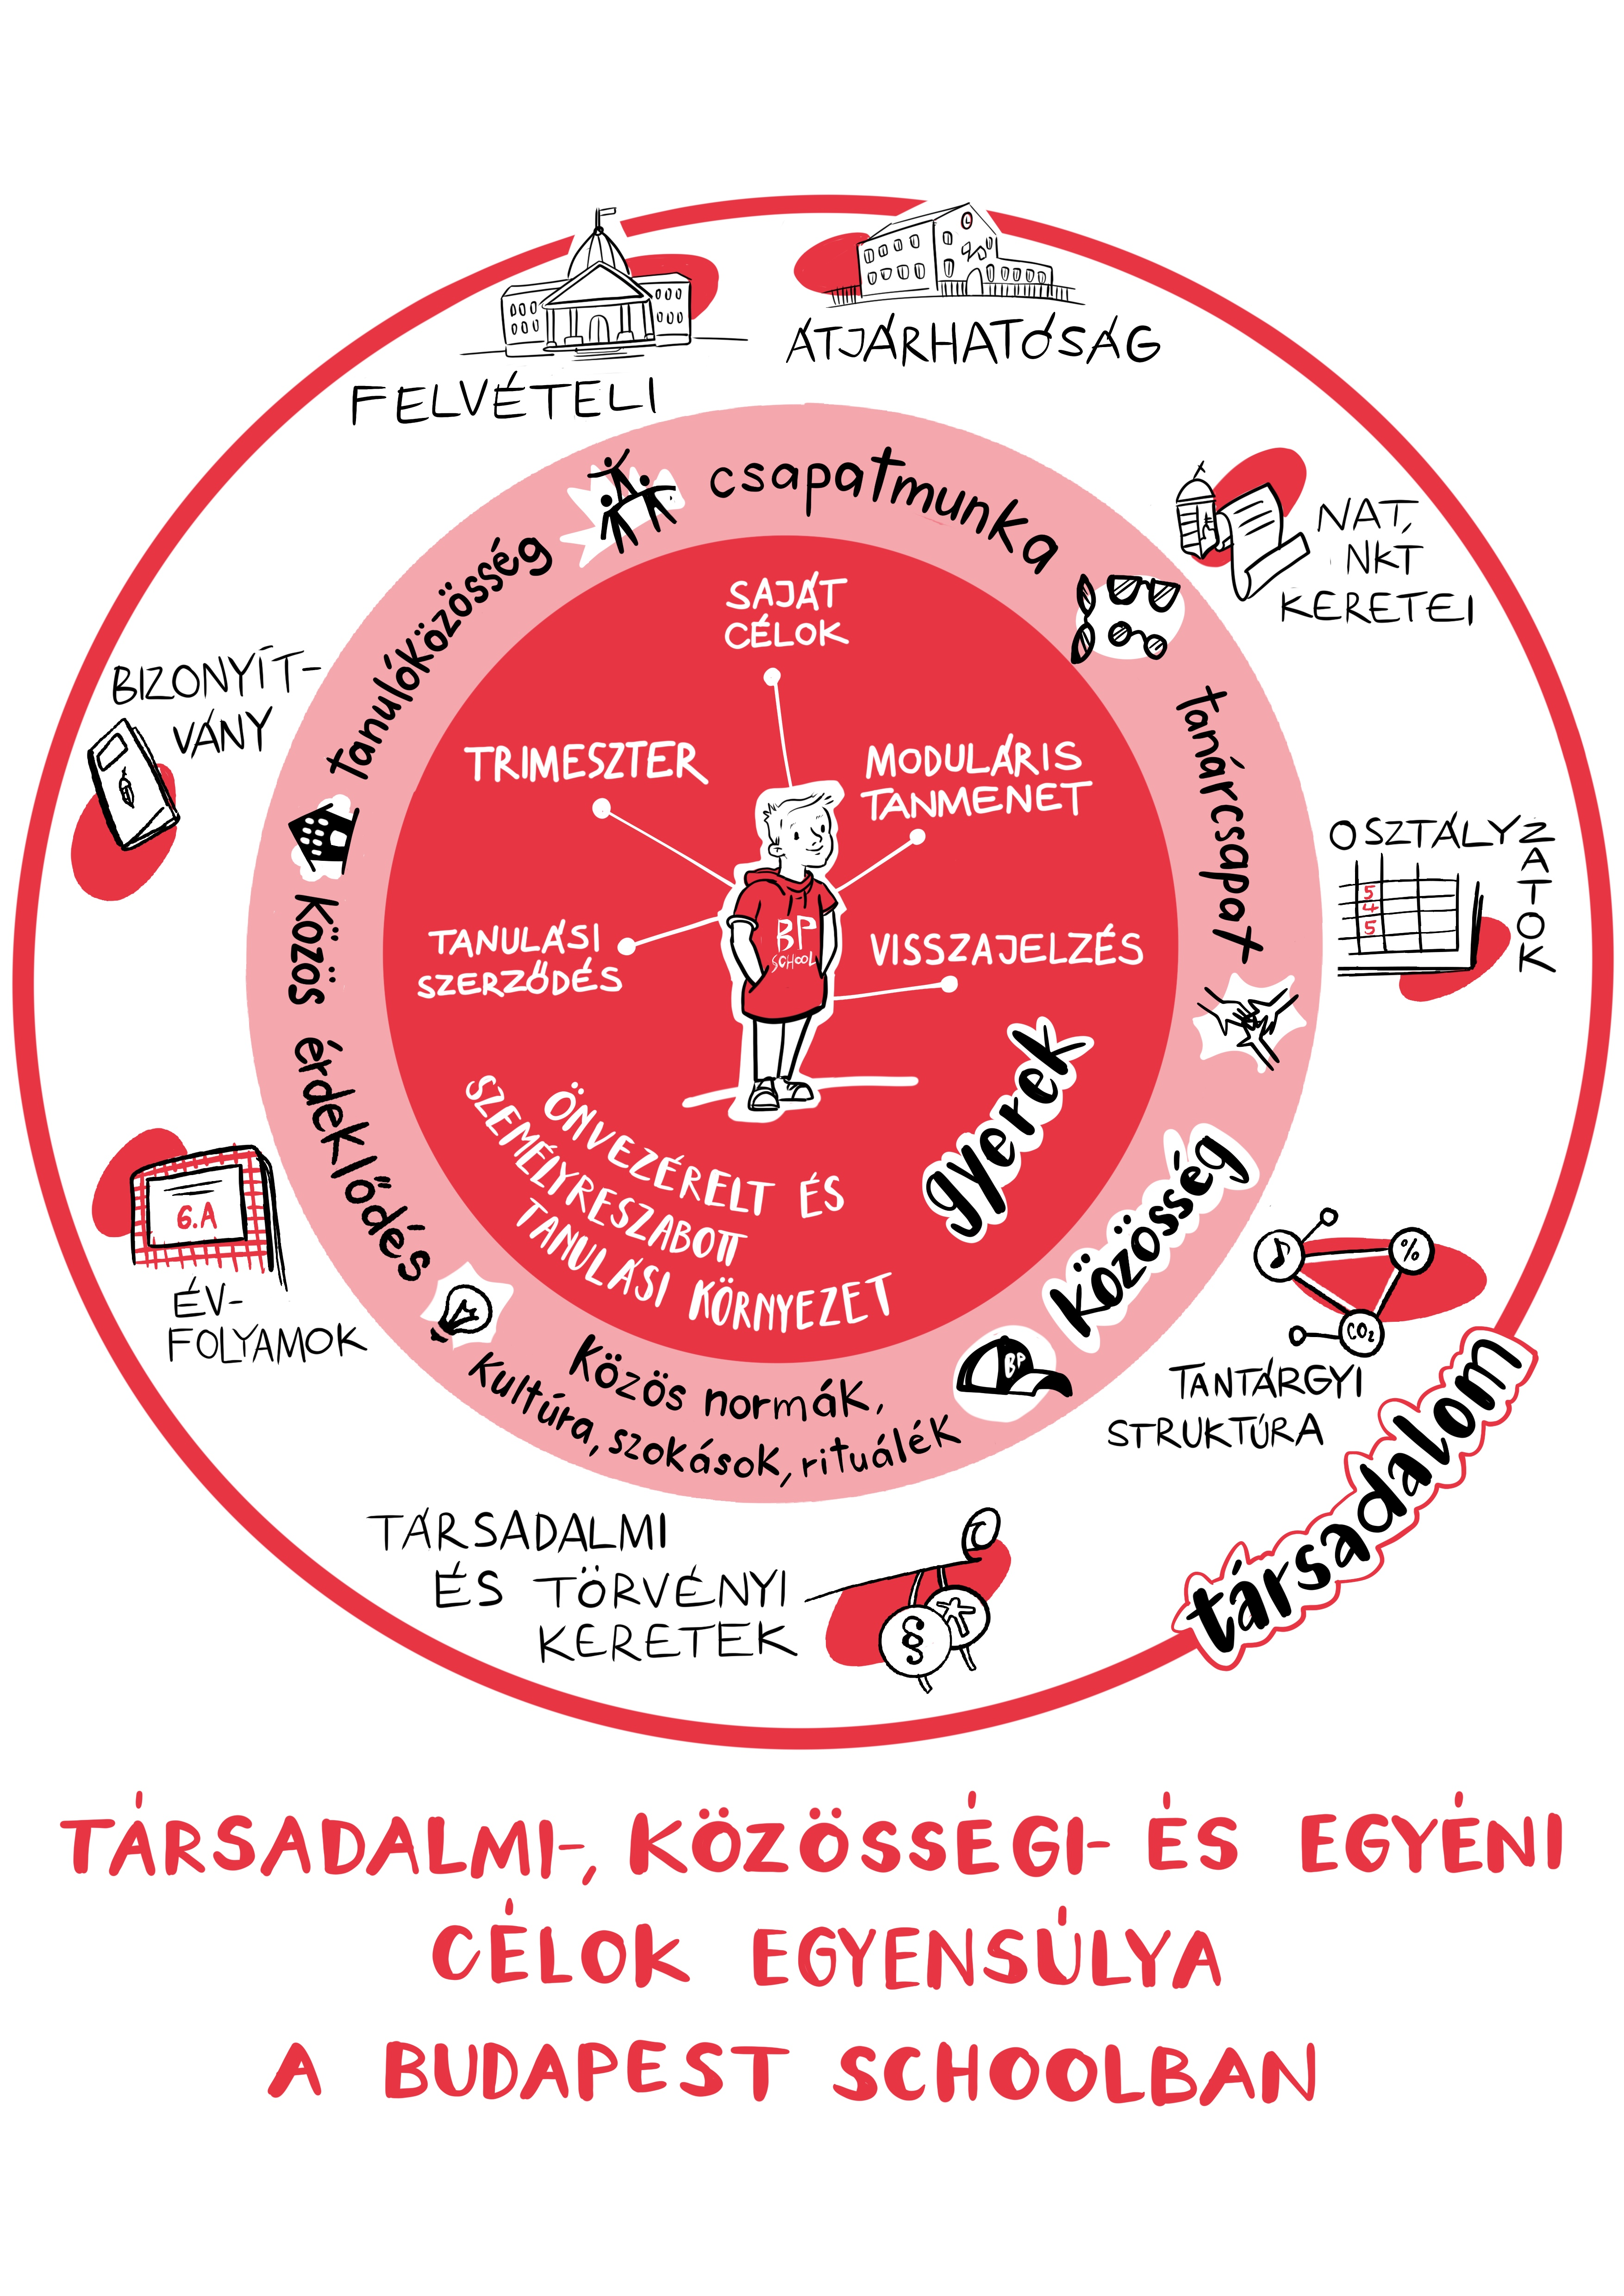
\includegraphics{pics/celok_egyensulya.jpg}
\caption{Egyéni és közösségi szempontok a Budapest School iskolában.}
\end{figure}

A Budapest School modellben az iskolának két rétege van. A gyerek
igényeire gyorsan reagáló tanulóközösség egy burok a gyerek körül. Ezt a
gyermekközpontú réteget veszi körül a társadalomhoz való kapcsolódást
biztosító külső réteg.

A belső burokban a Budapest School Modell a tanulás folyamatát
szabályozza, a \emph{Mit tanulunk?} kérdés helyett a \emph{Hogyan
szervezzük meg a tanulást?} kérdésre ad választ. A tanulás során a
gyerekek a Budapest School Modellben részletezett módon az
érdeklődésüknek megfelelően specifikus tanulási egységeket, vagyis
modulokat végeznek el, melyek eredményeit a saját portfóliójukban
gyűjtik össze. Így a gyerekek tanulási útja a portfólió fejlődésével
nyomon követhető, és a portfólió tartalma alapján megállapítható a
gyerek aktuális tudása, képessége. Az iskola fő funkciója emellett
mindvégig az aktív tanulás, saját fejlődésük kereteinek megtalálása, a
folyamatosan újragondolt saját célok állítása, és e célok irányába
történő haladás marad.

A belső réteg a személyre szabott és önvezérelt tanuláshoz szükséges
célkitűzés-tervezés, tanulás, és az arra történő reflektálás módját írja
le, vagyis a tanulás folyamatát rögzíti, míg annak pontos tartalmában
szabadságot enged.

\hypertarget{nat-hoz-a-kerettantervekhez-es-mas-kovetelmenyekhez-valo-kapcsolodas}{%
\subsection{A NAT-hoz, a kerettantervekhez és más követelményekhez\\ való
kapcsolódás}\label{nat-hoz-a-kerettantervekhez-es-mas-kovetelmenyekhez-valo-kapcsolodas}}

Ezt a szabadságot keretezik a társadalmi normák és jogszabályi
elvárások, hogy biztosítva legyen a gyerekek boldogulása a BPS iskolán
kívül is. Ezért a BPS modell alapján működő iskola programja a magyar
Nemzeti alaptanterv {\autocite{Nat2020}}, a miniszter által közreadott
kerettantervek {\autocite{Kerettanterv2020}} ismeretanyagát, azok
tantárgyi struktúráját és tanulási eredményeit teljes mértékben
tartalmazza. A BPS technikumok a szakmának megfelelő \emph{Képzési és
Kimeneti Követelményeket} veszik alapul.

Az iskolában sok mindent és sokféleképpen tanulhatnak a gyerekek. Azonban
a NAT, KKK által definiált tanulási eredmények elérése egy alap
minimumnak tekintendő, azok elérése mindenki számára kitűzött cél. Az
iskola szabadságot ad a gyerekeknek, tanároknak és szülőknek abban,\break
hogy
a gyerekek \emph{hogyan} érik el ezeket az elvárt eredményeket, és ezen
kívül fontos célnak tekinti, hogy a NAT ismeretanyagán túli világot is
megismerhessék a gyerekek.

\hypertarget{tantargyak-es-osztalyzatok}{%
\subsection{Tantárgyak és
osztályzatok}\label{tantargyak-es-osztalyzatok}}

A NAT és a miniszter által közreadott kerettantervekkel 100\%-ban
megegyező tantárgyi struktúra és a tanulási eredmények lehetővé teszik a
személyes portfóliók osztályzatokra váltását egy átlátható folyamaton
keresztül, amennyiben a gyerekeknek (szülőknek) a tantárgyankénti
osztályzatokra van szükségük (például továbbtanulás vagy ösztöndíj
miatt).

Technikumi képzés esetén a Képzési és Kimeneti Követelmények alapján
készült tantárgyak definiálják a szakmai képzés tartalmát.

A mindennapokban a tantárgyi érdemjegyeknél és osztályzatoknál\break
sokkal
részletesebb, több szempontot figyelembe vevő szöveges vagy
ér\-té\-ke\-lő\-táb\-lá\-zat- (rubric-) alapú visszajelzést kapnak a gyerekek. Ezek
bármikor
osztályzatokká konvertálhatóak egy algoritmus alkalmazásával
(\ref{evfolyam-osztalyzatok-bizonyitvany}. fejezet, \pageref{evfolyam-osztalyzatok-bizonyitvany}.~oldal).

A Budapest School Modell transzparenssé teszi az iskolában működő két
színtű struktúrát: a gyerekközpontú, személyre szabott, saját tervezésen
alapuló mindennapi tanulási élményt folyamatosan leképezzük a a NAT és a
kerettantervek tantárgyi struktúrájára. Az osztályzatok biztosítani
képesek az átjárhatóságot és a továbbtanuláshoz szükséges feltételeket.
A kettős rendszer, a személyre szabott belső tanulási környezet és a
kiszámíthatóságot adó külső kapcsolódások biztosítják, hogy az iskola
végén sikeres záróvizsgát (érettségi és technikusi) tegyenek.

\hypertarget{pedagogiai-modszersemlegesseg}{%
\subsection{Pedagógiai
módszersemlegesség}\label{pedagogiai-modszersemlegesseg}}

A Budapest School Modell a tanár feladatának tekinti, hogy mindig az
optimálisnak tűnő tanulási, tanítási, gyakorlási módszert válassza.
Ezért ez a modell nem beszél arról, hogy a modulokat (foglalkozásokat,
tanórákat) milyen pedagógiai módszer alapján szervezi a tanár. Van,
amikor egy frontális előadás a megfelelő, és van, amikor egy egy
drámával átitatott, koop módszer adja a legjobb eredményt.

A Budapest School Modell az iskolába járókat gyerekeknek hívja, a
tanulók és diákok szinonímájaként. Azok a gyerekek, akik tanulmányaik
vége felé felnőtté érnek a Budapest Schoolban, tanulók is maradnak, és
talán egy kicsit gyerekek is, ezért a szóhasználaton miattuk sem
változtatunk. Az ő esetükben a gyerek az iskolába járó tanulót jelenti.

\hypertarget{a-tanulni-tanulas-het-pillere}{%
\section{A tanulni tanulás hét
pillére}\label{a-tanulni-tanulas-het-pillere}}

A tanulás egyénenként változó, és ha vegyes korosztályokban is, mégis\break
egy közösségben valósul meg. \emph{A tanulni tanulás hét pillére\/} minden
korosztályban meghatározza a Budapest School működését.

\hypertarget{tanulni-tanulunk-fejlodeskozpontuak-vagyunk}{%
\subsection{Tanulni tanulunk --- fejlődésközpontúak
vagyunk}\label{tanulni-tanulunk-fejlodeskozpontuak-vagyunk}}

A BPS iskolában mindig ott, akkor és annak kell történnie a gyerekekkel,
ami őket a fejlődésükben a leginkább támogatja. Minden, ami az iskolában
történik, újra és újra erre az alapkérdésre kell, hogy visszatérjen. Az
segíti a leginkább a gyerekek fejlődését, amit most csinálunk, vagy
változtatnunk kell rajta? A Budapest School tehát rugalmas és
integratív, a gyerekek fejlődéséhez igazodó.

A gyerekek tanulása
% \href{https://pszichoforyou.hu/carol-s-dweck-minden-hiba-ujabb-lehetoseg-tanulasra/}
\emph{fejlődésközpontú
szemléletben} {\autocite{szabo:17}} (angolul: growth mindset) történik. Erőfeszítéseik
segítségével képességeik fejleszthetők, megváltoztathatóak, ha kellő
támogatást kapnak. Számukra inspiráló a kihívás, és a hibázás kevésbé
töri le lelkesedésüket. A gyerekek és a tanárok számára ezáltal nagyobb
fontossággal bír a tanulásba fektetett erőfeszítés és a fejlődés, mint
az aktuális teljesítmény.

A hibázás inkább válik a gyakorlás és az új megismerésének jelzőjévé.
Ennek feszültségmentes kezelése kulcsfontosságú abban, hogy a gyerekek
merjék feszegetni a saját határaikat, hogy magabiztosan dolgozzanak
azon, hogy képességeiket, ismereteiket vagy gyakorlataikat folyamatosan
fejlesszék. A hibázásból való tanulás fő célja, hogy mindig új hibákat
ismerjenek meg, és a korábbiakra minél jobb megoldásokat találjanak a
gyerekek.

\hypertarget{tanulni-tanulunk-sajat-celokat-allitunk}{%
\subsection{Tanulni tanulunk --- saját célokat
állítunk}\label{tanulni-tanulunk-sajat-celokat-allitunk}}

A gyerekek saját erősségeiket fejlesztve saját célokat állítanak, közben
céljaikat folyamatosan igazítják a világ adta lehetőségekhez és
szükségletekhez.

A tanulás egésze egy olyan folyamatként írható le, amely különböző
állomásokra, rövid célokra bontható. A tanulási célok állításának
folyamata, annak minősége az évek alatt folyamatosan változik, egyre
tudatosabbá, pontosabbá, komplexebbé válik. Ennek feltétele, hogy már az
első évektől el kell kezdeni az életkornak és személyes
lehetőségeknek megfelelő célállítás gyakorlását.

A gyerekek jellemzője a kíváncsiság, az igény a felfedezésre,
tapasztalásra. A BPS-gyerekek számára \emph{a tanulás egy önvezérelt aktív
folyamat}, melynek megtartása és folyamatos fejlesztése a Budapest
School tanárainak legfőbb feladata. Nem csak azokra a képességekre
fókuszálunk, amelyekre ma szükségük van, mert így tudásuk veszítene a
világ változásával a korszerűségéből. Az iskola abban segíti őket, hogy
megtaníthassák maguknak azokat a képességeket, amelyekre épp az adott
élethelyzetükben szükségük lesz. A tanulás így élményszerűvé válik,
ismeretszerző jellege csökken, és nő az önálló felfedezés lehetősége.

\hypertarget{tanulni-tanulunk-mindig-es-mindenhol}{%
\subsection{Tanulni tanulunk --- mindig és
mindenhol}\label{tanulni-tanulunk-mindig-es-mindenhol}}

A tanulásra a Budapest Schoolban mindig van lehetőség. A tanulási
környezet pontos kialakítása a gyerekek igényeitől, fejlettségi
szintjétől és\break
korosztályától is függ. A tanulási rend meghatározásáért a
BPS tanulásszervezői felelnek.

A tanulás során jut idő egyéni és csoportos, gyakorló, ismeretszerző és
alkotó foglalkozásokra is. A tanulási egységek között van idő
fellélegezni és felkészülni az újabb modulokra. Van, amikor az is
megoldható, hogy a gyerekek és tanárok újratervezzék az időrendjüket, ha
egy tanulási egység nagyon magával ragadja a gyerekeket, és nagyon benne
maradnának abban a tevékenységben.

A tanulás az iskolában nem ér véget. A tanulás szeretetének
kialakulásával folyamatossá válik az ezzel való foglalkozás, így a
Budapest School tanulásnak tekinti az otthon vagy a szünetekben
tanulással eltöltött időt is, ahol néha hatékonyabb módon tud egy gyerek
gyakorolni, kutatni, alkotni, mint az iskolában, amikor társaival van
egy közösségben és ezáltal számos más inger is éri.

Az iskolában történő tanulással egyenrangúnak tekintjük az otthon\break
tanulást, az iskolától független iskola utáni programokat, a (nyári)
táborokat, a családi utazásokat, a vállalatoknál töltött gyakornoki
időt, az egyéni tanulást és projekteket. A tanulás bárhol és bármikor
történhet, amíg az eléri a célját. Célunk, hogy a gyerekek mindenhol és
mindig tanuljanak.

\hypertarget{tanulni-tanulunk-egyutt-egymastol}{%
\subsection{Tanulni tanulunk --- együtt,
egymástól}\label{tanulni-tanulunk-egyutt-egymastol}}

A tanulás egyénileg és csoportokban is történhet. A csoportok
megszervezése mindig azon múlik, hogy az adott tanulási célt mi
szolgálja a legjobban. Ennek megfelelően a gyerekek nem állandó, hanem a
tanulási célokhoz, az érdeklődéshez, a képességi szintekhez alkalmazkodó
rugalmas csoportokban tanulnak. A tanulás ezáltal kevert korcsoportokban
is történhet, akár egy nagy családban. Együtt, egymástól tanulnak a
gyerekek, egymást segítik a fejlődésben. Az egymásnak adott
visszajelzések, megerősítések révén folyamatosan alakul ki a tanulás
tisztelete és a képességek fejlesztésébe vetett hit, az együttműködésre
és az alkalmazkodásra való képesség.

A közösségben tanulás módja nagyban függhet attól, hogy egy gyerek
mennyire zárkózott, mennyire tud és akar önállóan tanulni. A csoportos
munkák során alapelv, hogy a zárkózott gyerekek is lehetőséget kapjanak,
hogy csöndesen vagy kisebb csoportban végezhessék a munkájukat,
mondhassák el ötleteiket. Az egyéni tanulásban minden gyereknek
lehetőséget kell adni arra, és segíteni kell abban, hogy önállóan,
fókuszáltan tudjon tanulni.

\hypertarget{tanulni-tanulunk-alkotunk-es-felfedezunk}{%
\subsection{Tanulni tanulunk --- alkotunk és
felfedezünk}\label{tanulni-tanulunk-alkotunk-es-felfedezunk}}

A tanulás három rétege, az ismeretszerzés, a gondolkodás fejlesztése és
az alkotás egyszerre jelenik meg a Budapest School mindennapjaiban. Az
alkotó munka rugalmas időkereteket, változó csoportbontásokat, és a
projektmódszerek sokszínű alkalmazását igényli. A tanulás ilyenkor
sokszor inkább alkotássá válik, az ismeret pedig termékké változik.

A gyerekek önmaguk és a világ számára releváns kérdésekkel foglalkoznak,
amihez külső szakértőket is bevonnak, ha szükséges. A tanulás tehát
célokhoz, nem pedig tárgyakhoz kötött. A tanulás tartalmát igazítjuk a
tanulás céljához, ezáltal az egyes tudományterületek, művészetek, vagy
épp mesterségek gyakran keverednek egymással egy-egy modulon belül.
Szintén a célhoz igazított tanuláshoz kötődik a kutató-felfedező
attitűd, ami az ismeretlen felfedezésére, a megválaszolhatatlan
megválaszolására irányul.

\vspace*{.5ex}
\hypertarget{tanulni-tanulunk-egymasra-figyelunk}{%
\subsection{Tanulni tanulunk --- egymásra
figyelünk}\label{tanulni-tanulunk-egymasra-figyelunk}}

A gyerekek tanulását családi hátterük változása, egyéni problémák,
számos mindennapi esemény befolyásolhatja. Ezek figyelembevétele a
mindennapokban, a \emph{mentortanárral} való bizalmi viszonynak
köszönhetően válik lehetségessé. Ennek a kapcsolatnak az alapjait ezért
a partnerség, az értő figyelem adja.

A Budapest School emellett kiemelt figyelmet fordít arra, hogy a sajátos
nevelési igényű tanulók is lehetőséget kapjanak a csoportban való
munkára, amennyiben az a közösség számára is hasznos. Tanulásukat, ha
szükséges, külső szakember segíti. A Budapest School a hátrányos
helyzetű gyerekek számára is biztosítani kívánja az elfogadó, fejlesztő
környezetet. Az egyenlő bánásmód megvalósulása érdekében olyan
differenciált tanulási környezetet alakít ki, ami biztosítja a minél
nagyobb mértékű inkluzivitást.

\vspace*{.5ex}
\hypertarget{tanulni-tanulunk-tanulva-tanitunk}{%
\subsection{Tanulni tanulunk --- tanulva
tanítunk}\label{tanulni-tanulunk-tanulva-tanitunk}}

A Budapest School \emph{tanulásszervezői} partnerként, a tanulás
folyamán segítő társként vannak jelen a gyerekek életében. A tanulás
tanórák helyett pontos tanulási célokat tartalmazó tanulási modulokból
épül fel, melyek során a tanár az adott cél eléréséhez szükséges
eszközöket, tanulási segédleteket biztosítja.

A tanár akkor és annyira segíti a gyerekeket a saját céljuk elérésében,
amennyire az épp szükséges, és folyamatosan tekintettel van arra, amit a
gyerek saját fejlődési üteme megkíván. Ehhez tudatosan kell kezelnie
nemcsak a gyerekeket érintő fejlesztési lehetőségeket, hanem azt is
pontosan látnia kell, hogy egy adott tanulási cél elérésének milyen
készségszintű vagy gyakorlatias alapfeltételei vannak. Ezért a gyerekek
tanulási célját támogatandó segítenie kell abban, hogy a gyakorló idő,
az alkotó idő és az új ismeret megszerzésének ideje folyamatos
egyensúlyban legyen. A tanár a gyerekekkel együtt fejlődik, saját
tanulása a segítői szerepben folytonos.

\hypertarget{emberkep}{%
\section{Emberkép}\label{emberkep}}

A világ és benne az egyén állandóan változik, és a változás mégis számos
állandóságot jelöl ki. Korábban a technológiai változás évszázadokban
volt mérhető, az általunk használt eszközök száma és komplexitása jóval
kisebb volt, mára néhány év, vagy egy pár órás repülőút elegendő ahhoz,
hogy olyan környezetbe, olyan emberek, eszközök közé kerüljünk, ahol
másként kell alkalmazkodnunk, mint ahogy azt tanultuk. Ebben a világban
a saját belső harmóniánk megtalálása, a saját közösségünkhöz,
közösségeinkhez való kapcsolódás, a világ működésének megértése és a
törekvés arra, hogy tegyünk a fenntartásáért, különösen fontossá vált.
Ahhoz, hogy ezeknek a változásoknak meg tudjunk felelni, a tanári,
szülői és a tanulói szerepekben is folyamatos fejlődésre van szükségünk.
A jövőbe nem látunk, de egy dolgot biztosan tudunk: bármilyenek
lesznek is a jövő kihívásai, nekünk az a fontos, hogy ez a gyerekek számára
ne félelmetes és szorongást keltő legyen, hanem lehetőséget, kihívást és
örömet okozzon.

Azt szeretnénk, hogy a fiatalok az iskolában és utána is könnyen
megtalálják a saját útjukat. Képesek legyenek önmaguknak célokat
állítani, azokat elérni. Képesek legyenek már kisgyerekkortól
sajátjukként megélni a tanulást, és ahhoz kapcsolódóan célokat elérni, és
fokozatosan tanulják meg azt, hogy egyénileg és csoportosan is tudjanak
nagyszabású projekteket véghezvinni. A tanulás három rétege, a tudás
megszerzése, az annak felhasználását segítő önálló gondolkodás és az
alkotás egyszerre jelenik meg a mindennapokban. Ezek egyensúlyban
tartása éppoly fontos, mint az, hogy a gyerekek a kerettantervben
szereplő tanulási eredményeket és a további célkitűzéseiket egyaránt
sajátjukként éljék meg, ezzel is biztosítva, hogy személyes céljaik és a
társadalmi elvárások folyamatos egyensúlyban lehessenek.

Ezért \emph{legfontosabb fejlődési dimenziónak az önálló, célorientált
tanulási és stratégiai gondolkodást tekintjük}, melynek ütemeit tanulási
szakaszokra bontjuk. A társas kapcsolatok tanulási folyamatában a
születéstől a felnőttkorig a teljes magára hagyatottság és énközpontúság
csecsemőkori állapotából fejlődik az ember önállóan és kreatívan
gondolkodó, önmagával és közösségével integránsan élő, érett nagykorúig.
Ezt az utat Erik Erikson pszichoszociális fejlődési modelljében
rögzítette {\autocite{Erikson1991}}. A Budapest School ezt a modellt
integrálja tanulási struktúrájába, melynek eredményeképp az
iskolakezdőtől az érettségizőig négy tanulási szakaszt különít el. Ezen
tanulási szakaszok határait az önállósodás során tapasztalt egyéni
mérföldkövek jelölik ki, melyek fokmérője a saját cél állításának
képessége, illetve a célkitűzés időbeli és tartalmi realitása, valamint a
közösséghez való kapcsolódása. Amellett, hogy az egyes tanulási
szakaszok a célállításban elkülönülnek egymástól, a szintugrás abban is
mérhető, hogy mennyire képes egy gyerek az alatta lévő szinten lévő
társait segíteni az előrelépésben. A folyamatos kortárs támogatás a
szintekben való előrehaladás valós fokmérője a mentor és a szülő
visszajelzései mellett.

Az egyes szintek közötti életkori határok elmosódnak, kontúrjaik nem
élesen válnak el egymástól, így inkább a fejlődés iránya, mintsem a
korosztályi tagolás a fontos. Számos kutatás bizonyítja, hogy a gyerekek
mentális életkora és az egyes területeken való fejlettsége között
jelentős különbségek lehetnek. Vagyis előfordulhat, hogy egy gyerek
zongorázásából már jóval előrehaladottabb célokat tud kitűzni maga elé,
mint olvasásból vagy épp robotikából, és ez rendben van így.

\hypertarget{elso-szakasz-5-10-ev}{%
\paragraph{Első szakasz, 5--10.\ év}\label{elso-szakasz-5-10-ev}}

Ebben a korban alakul ki a gyerekek logikus gondolkodása, melynek
részeként feladatokat tudnak rendszerezni, sorrendeket képesek
felállítani, és azokat fogalmakhoz társítani. A gondolkodásuk elkezd a
befelé fordulóból a társas kapcsolatok irányába nyílni, ezáltal
megnyílik a közösségi problémamegoldás lehetősége. Igényük nő a belső és
a külső rendezettségre, így elkezdhetnek önmaguk szabályokat alakítani a
saját tanulási igényeik kapcsán. Az első szakaszban a gyerekek
pszichoszociális fejlődésükkel összhangban a saját maguknak állított cél
jelentőségének fogalmát tanulják rövid, eleinte néhány órás, majd a
szakasz vége felé néhány napos tervezéssel, és erre adott önreflexiókkal
és külső megerősítésekkel. Megtanulják a ma, a tegnap és a holnap
fogalmát. Tanulási szerződésük tartalmát eleinte főleg a mentor és a
szülő segítségével állítják össze, hogy annak a szakasznak végére már
teljesen egyedi, önállóan kiválasztott elemei is lehessenek.

Ebben a szakaszban a szabad játéknak nagy szerepe van, a belső világ
tágassága fokozatosan nyílik meg a külvilág felé, és kezd lényegessé
válni az azokkal való kommunikáció kiérlelése. Ekkor tanulnak meg a
gyerekek írni, olvasni, és megismerik a matematikai alapműveleteket,
valamint a mindennapjaikban használatos geometriai és kombinatorikai
alapfogalmakat. Célunk, hogy önmagukhoz és környezetükhöz érzékenyen,
odafigyeléssel és empátiával forduljanak, megtanulják tiszteletben
tartani, hogy társaik másmilyenek, akiket más dolgok is érdekelhetnek,
másfajta megoldásaik is lehetnek. \emph{A szakasz végére biztonsággal
meg tudnak maguknak tervezni egy néhány napos projektet.}

\hypertarget{masodik-szakasz-914-ev}{%
\paragraph{Második szakasz, 9--14.\ év}\label{masodik-szakasz-914-ev}}

A gyerek testi és pszichoszociális fejlődése szempontjából egyaránt
kiemelten fontos időszak következik. A korai serdülőkorban alakulnak ki
a másodlagos nemi jellegek, melyek ütemükben mind a fiúk és lányok, mind
az egyének között jelentős eltéréseket mutathatnak. Az egyéni tanulási
tervek összeállításának ezért ebben az időszakban megnő a szerepe.

Az agyi struktúrák jelentős átalakulása is erre az időszakra tehető, a
gondolkodás, a figyelem, az emlékezet területén is lehetnek ezen
átalakulások miatt nehézségek, amelyeket később, --- az átmeneti
visszaesést követően --- az agy fejlettebb működése követ. Ekkor
alapozhatja meg egy gyerek a tervezés, a saját tanulási célok komplexebb
fogalmait. Aki ebbe a szakaszba lép, már hetekre előre ki tudja jelölni
a saját feladatait. Három év alatt oda kell eljutni, hogy a szakasz
végére önállóan képes legyen egy teljes trimeszternyi tanulási tervet
összeállítani. Ehhez a hetek számát folyamatosan növelnie kell, miközben
a problémák komplexitása is változik. A szülő még mindig megjelenik a
célalkotásban, de egyre inkább átalakul a szerepe tanácsadóvá. A mentor
az egyéni fejlődés mintázataira figyelve segíti a gyereket abban, hogy
fejlettségi szintjének, aktuális testi, lelki változásainak megfelelő
módon legyen terhelve.

\emph{A szakasz végén önállóan be tudja mutatni társainak egy pár hetes
projekt eredményeit, és mind szövegértése, mind logikus gondolkodása és
matematikai alapismeretei olyan szinten állnak, hogy elmélyült alkotó,
kutató feladatokat vállalhat a következő szakaszban.} Biztonságos
nyelvhasználata a sajátja mellett egy másik nyelvben is elindul, és
értékrendjében önmaga és társai megismerésén túl a környezet és a világ
fogalma is tágulni kezd.

\hypertarget{harmadik-szakasz-1216-ev}{%
\paragraph{Harmadik szakasz, 12--16.\
év}\label{harmadik-szakasz-1216-ev}}

A sajátként megélt tanulási célok eddigi alapozása ebben a szakaszban
nyeri el mélyebb funkcióját. A tinédzserkor minden szempontból a gyerek
kivirágzásának időpontja, melynek során a helyét kereső, befelé, saját
változásaira fókuszáló gyerekből egy, a jövő felé nyitott kamasz válhat.
A gondolkodási struktúrák mellett megnő a családon túli társas
kapcsolatok szerepe, és ekkor fontos, hogy a családias jelleg, a
biztonságos tanulás, a szülővel való konzultáció mint a gyerek számára
egyaránt fontos érték, és nem mint kényszer jelenjen meg. Az érvelés, a
hipotézis-alapú problémamegoldás, valamint a jelen fókuszált megélése
ebben a korban alakul ki, ahogy annak a tudata is, hogy tetteinknek a
jövőre nézve nagyobb mértékű következményei lehetnek. Kiemelten fontos
ebben a szakaszban a különböző vélemények, információk, megoldási
lehetőségek számbavétele, annak lehetősége, hogy a gyerek egyénileg
ismerhesse fel az eltérő utak közötti különbségeket, és ha teheti,
kérdőjelezzen meg akár tudományos hipotéziseket, vagy írjon újra
művészeti, kulturális tartalmakat. Ha a gyerek ezen határok megértésében
szabadon fejlődik, akkor lehetősége lesz arra, hogy a megszerzett
alapképességeit olyan kreatív irányokba fordíthassa, melyek saját élete
és társadalmunk jövője formálásához egyaránt hasznosak lehetnek.
\emph{Ebben az időszakban a saját tanulási célokat egy teljes
trimeszterre vonatkozóan egyénileg határozza meg a gyerek, a szülő és a
mentor ebben a folyamatban mint konzulens jelennek meg. Meghozza első
komolyabb döntéseit arról, hogy milyen területekkel szeretne
elmélyültebben foglalkozni, és ehhez kapcsolódóan választott érettségi
tantárgyait is kijelöli a szakasz végére.} Előadásmódját, kutatási és
alkotói munkáját felnőtt jegyek jellemzik.

\hypertarget{negyedik-szakasz-1519-ev}{%
\paragraph{Negyedik szakasz, 15--19.\
év}\label{negyedik-szakasz-1519-ev}}

Ebben a szakaszban a gyerek fizikai értelemben teljesen felnőtté válik,
ehhez kiemelten szüksége van érzelmi és szociális biztonságra. A
szerelem, a szexuális identitás erősödése, az önállósodásra való igény,
az addikciók veszélye konfliktusokat szülhet, amelyek kezelése különösen
fontos ebben az időszakban. Az iskola (elsősorban a mentor) a szülővel
együttműködve tudja megteremteni ezt a biztonságos közeget.

A szakasz célja, hogy a gyerek képessé váljon a saját életét
meghatározó, egy-két éves távlatokban mérhető felelős döntések
meghozatalára, melyek akár sorsfordító jelentőségűek is lehetnek. Ezek a
döntések vonatkozhatnak egy emelt szintű érettségire való felkészülésre,
egy nemzetközi egyetemre való felkészülésre, egy nagyobb komplexitású
kutatási vagy alkotói projektre. Fontos azonban a gyerek támogatása
abban is, hogy beláthassa, nem kell örök érvényű döntéseket hoznia.
Ekkorra már megtanult szakaszosan célokat állítani, és tudja, hogy
bármikor lesz lehetősége az életben újratervezni. Önállóan készül az
érettségire, tanárai segítik, hogy folyamatosan megtalálja a kihívást
ebben. Saját céljai szűkebb környezetén túl könnyedén hatással lehetnek
már a világra is.

\hypertarget{kapcsolat-a-hazai-es-nemzetkozi-oktatasi-iranyzatokkal}{%
\section{Kapcsolat a hazai és nemzetközi oktatási
irányzatokkal}\label{kapcsolat-a-hazai-es-nemzetkozi-oktatasi-iranyzatokkal}}

A Budapest School programja a hazai és nemzetközi oktatási reformok
kontextusában és a pszichológia, a szociálpszichológia, valamint a
szervezetfejlesztés terén elvégzett kortárs kutatások tükrében válik
könnyebben értelmezhetővé.

Magyarországról több iskola története, működése is nagy hatással volt
ránk. A 90-es évektől induló alternatív iskolák világát mi a
% \href{https://www.rogersiskola.hu/}
{\emph{Rogers Személyközpontú
Általános Iskola}}, a %\href{https://www.lauder.hu/wp/}
{\emph{Lauder
Javne Iskola}}, a
% \href{https://www.kincskereso-iskola.hu/}
{\emph{Kincskereső Iskola}} és
a %\href{https://gyermekekhaza.hu/}
{\emph{Gyermekek Háza}} alapján
ismertük meg. A megújuló középiskolák modelljének mi az
% \href{https://www.akg.hu/}
{\emph{Alternatív Közgazdasági Gimnáziumot}}
és a %\href{https://poli.hu/wp/}
{\emph{Közgazdasági Politechnikumot}}
tartjuk. Ezek az iskolák a személyközpontúság, a gyerekközpontúság
hangsúlyozása mellett elkezdték a gyakorlatban alkalmazni a partnerség
alapú kommunikációt, a differenciálás, a kooperatív technikák módszerét
és egyes projektmódszertanokat.

Programunk kidolgozásában nagy szerepe volt annak, hogy ezek az iskolák
olyan szemléletmódbeli alapokat fektettek le, amelyek mára
alapelvárásként fogalmazódnak meg a szülők oldaláról az iskolákkal
szemben.

Gyakorlati tapasztalatokat a világ más részein is gyűjtöttünk. A 21.
században a Budapest Schoolhoz hasonló kezdeményezések sorra indulnak a
világban. Ezek egyes jegyei a Budapest School modelljével összhangban
vannak:

A %\href{https://wildflowerschools.org/}
{\emph{Wildflower School}}
tanulóközösségek hálózatát működteti kisebb üzlethelyiségekben. A
Budapest Schoolhoz hasonlóan célja, hogy falakat\break
romboljon a gyerekek és
a világ között: az egyéni tanulás és az intézményes tanulás, a tanár és
a tudós szerepe, valamint az iskola és környezete közötti határok
elmosása az egyik fő üzenete.

Hasonlóan az otthon tanulás és az \emph{unschooling} strukturált
formáját keresi az amerikai Texasban alapított
%\href{https://www.actonacademy.org/}
{\emph{Acton Academy}}, amely a
szokratikus módszereket (azaz, hogy megbeszéljük közösen), a valós
projektből való tanulást, és a gyakornokoskodáshoz hasonló munka közbeni
tanulást („learning on the job'') teszi a megközelítésének középpontjába.

A %\href{https://www.hightechhigh.org/}
{\emph{High Tech High}} iskoláiban
a gyerekek elsősorban projektmódszertan alapján tanulnak. A tanulási
jogokban való egyenlőség mellett az egyéni célokra szabott tanulás, a
világ alakulásához kapcsolódó tartalmi elemek, valamint az
együttműködés-alapú tanulás is megjelenik pedagógiájukban a Budapest
School által is alkalmazott jegyekből.

A %\href{https://www.school21.org.uk/}
{\emph{School21}} brit iskola
21.~századi képességek fejlesztését tűzte ki célul. Ezért a
prezentációs, előadói skillek kiemelt jelentőségűek. Az iskola
egyensúlyt akar teremteni a tudásbéli (akadémiai), a szívbéli
(személyiség és jóllét) és a kézzel fogható (problémamegoldó, alkotó)
között. A Budapest School iskoláinak hasonló módon célja, hogy a tanulás
három rétegét, a tudást, a gondolkodást és az alkotást folyamatos
harmóniában tartsa.

A %\href{https://khanlabschool.org/}
{\emph{Khan Lab School}} a
Montessori-módszert keveri az online tanulással. Kevert korosztályú
csoportokban, személyre szabott módszerekkel segítik a
képességfejlesztést és a projektalapú munkát. A BPS modell négy tanulási
szakasza tulajdonképpen megfelel a Khan Lab School
%\href{https://khanlabschool.org/independence-levels}
{\emph{függetlenségi
szintjeinek}}.

\chapter{A tanulás megközelítése}
\hypertarget{pedagogiai-es-pszichologiai-hatter}{%
\section{Pedagógiai és pszichológiai
háttér}\label{pedagogiai-es-pszichologiai-hatter}}

Az iskolák működésének tanulmányozása mellett a Budapest School komoly
tudományos-elméleti háttérre alapozta koncepcióját.

Ezek közül is oktatási programjának központjában
%\href{http://tantrend.hu/hir/fejlodeskozpontu-szemlelet-az-iskolaban}
{Carol
Dweck fejlődésközpontú szemlélete} {\autocite{gerencser:18}}
áll. Emellett nagy hangsúlyt
fektetünk az alábbi elméletek gyakorlati alkalmazására is:

Reformpedagógiai irányzatok elméletei, különös tekintettel:

\begin{itemize}
\tightlist
\item
  Montessori-pedagógia (Maria Montessori),
\item
  kritikai pedagógia (Paulo Freire)
\item
  élménypedagógia (John Dewey)
\item
  felfedeztető tanulás (Jerome Bruner)
\item
  projektmódszer (William Kilpatrick)
\item
  kooperatív tanulás (Spencer Kagan)
\end{itemize}

Pszichológia és szociálpszichológiai kutatások eredményei:

\begin{itemize}
\tightlist
\item
  kognitív interakcionista tanuláselmélet (Jean Piaget)
\item
  személyközpontú pszichológia (Carl Rogers)
\item
  kommunikáció és konfliktuskezelés (Thomas Gordon)
\item
  erőszakmentes kommunikáció (Marshall Rosenberg)
\item
  pozitív pszichológia eredményei, különös tekintettel: flow-elmélet,
  kreativitás-kutatások (Csíkszentmihályi Mihály)
\item
  érzelmi és társas intelligencia (Peter Salovey, John D. Mayer, Daniel
  Goleman)
\item
  motivációkutatások; ezeket jól foglalja össze Daniel H. Pink műve
  % Motiváció 3.0 műve % LK: ???
  {\autocite{Pink2011}}
\item
  hősiesség pszichológiai alapjai (Phil Zimbardo)
\item
  fejlődésfókuszú szemlélet (Carol Dweck)
\end{itemize}

\hypertarget{pedagogiai-modszerek}{%
\section{Pedagógiai módszerek}\label{pedagogiai-modszerek}}

A Budapest School iskola tanárainak feladata, hogy mindig keressék azt a
módszert, azt a környezetet, ami az adott gyerekekkel, adott
környezetben, adott időben a leginkább működik. Nem tudjuk megmondani
előre, hogy mikor milyen módszert érdemes választani, de azt tudjuk,
hogy mi alapján keressük a megfelelő technikákat. Vannak olyan
módszerek, amelyek a saját célok lehetőségeinek kitágítását és azok
elérését nagyban támogatják. Ezek alkalmazása javasolt a csoportmunkák
és az egyéni gyakorlások alatt.

Azt is tudjuk, hogy nem baj, ha nem elsőre találtuk meg a megfelelő
módszert, mert a próbálkozások során rengeteg új információt nyerünk,
amelyek segítségével már könnyebb megtalálni a valóban megfelelő
megoldást. Az alábbiakban néhány a Budapest School számára meghatározó
fontosságú módszert emelünk ki.

\hypertarget{rugalmas-csoportbontasok}{%
\subsection{Rugalmas csoportbontások}\label{rugalmas-csoportbontasok}}

Pedagógiai elvek az osztályok, csoportbontások, foglalkozások
megszervezése tekintetében A BPS Általános Iskola és Gimnázium az Nkt.
4. § 24. pontjában, 25. § (7) bekezdésében, 26. §-ában, 31. § (1), (2)
bekezdésében valamint a 20/2012. EMMI rendelet 13. § (1) bekezdésében
foglalt felhatalmazása alapján a 20/2012. (VIII. 31.) EMMI rendelet 2.
mellékletében definiált eltérő pedagógiai elveket, valamint a 20/2012.
(VIII. 31.) EMMI rendelet 7.§ (4) bekezdése szerint definiált eltérő
pedagógiai módszereket alkalmaz. A fentiek alapján a BPS csoportbontási
és foglalkozás-szervezési elvei a következők:

\begin{itemize}
\tightlist
\item
  alsó tagozaton összevont osztály megszervezése lehetséges;
\item
  az osztályok létszámára vonatkozó minimális rendelkezéseket nem
  alkalmazza a BPS;
\item
  a tanórákat és foglalkozásokat a BPS van, hogy különböző évfolyamok,
  különböző osztályok tanulóiból álló csoportok részére szervezi meg és
  van, amikor egy évfolyamra járó gyerekek csoportjának, azaz főleg az
  osztályoknak szervez egy foglalkozást;
\item
  a BPS alkalmazza a projektoktatás módszerét, melynek során a
  témaegységek feldolgozása, a feladat megoldása a tanulók
  érdeklődésére, a tanulók és a pedagógusok közös tevékenységére,
  együttműködésére épül.
\end{itemize}

Magyarul megfogalmazva: a gyerekeket a tanároknak úgy kell csoportokra
bontaniuk, ahogy ez szerintük a leginkább támogatja a gyerekek tanulását.
Ha egy 10 éves gyerek jól tud egy 14 éves gyerektől tanulni, és mindenki
élvezi ezt, akkor egy kevert korosztályú, kooperatív differenciálás a
legcélrevezetőbb. Egy emeltszíntű matematika érettségire felkészítő
csoportban célszerű az egy tudásszinten lévő gyerekeket egy csoportba
tenni.

Tehát amennyiben a különböző évfolyamra járó gyerekek oktatása az adott
tantárgyat, foglalkozást vagy modult illetően hatékonyabb az
évfolyamonkénti csoportokban történő oktatással szemben, úgy olyan
csoportok kialakíthatók, amelyekben a legidősebb és a legfiatalabb
gyerek évfolyamának különbsége hatnál nem több.

A különböző évfolyamra járó gyerekek csoportmunkája során is figyelemmel
kell lenni a tanulók életkori sajátosságaira. A tanárnak differnciálni
kell. Leginkább abban, hogy az eltérő évfolyamszinten lévő gyerekeknek
eltérő tanulási eredmények elérése a célja.

A csoportok összeállításakor figyelembe kell venni a közösség minden
tagjának, és minden csoportjának, így az osztályok, évfolyamok és
tanulóközösségek érdekeit.

\hypertarget{projektmodszer}{%
\subsection{Projektmódszer}\label{projektmodszer}}

Projektmódszert alkalmazó modulok során fő célunk, hogy a gyerekek
aktívak és kreatívak legyenek, és ezért a tevékenységek sokszínűségét
helyezzük fókuszba. Projektmódszer alkalmazásakor is arra bíztatjuk a
tanárokat, hogy a legváltozatosabb és legadekvátabb módszereket
alkalmazzák.

\hypertarget{a-projektmunka-folyamata}{%
\subsubsection{A projektmunka
folyamata}\label{a-projektmunka-folyamata}}

\hypertarget{tema-cel}{%
\paragraph{Téma, cél}\label{tema-cel}}

Az első lépés a projekt céljának és tartalmának meghatározása. Erre
javaslatot tehet a tanár, a gyerekek vagy akár egy szülő is. Fontos,
hogy a gyerekek a projekt témáját vagy célját már önmagában értelmesnek,
relevánsnak tartsák.

\hypertarget{otletroham}{%
\paragraph{Ötletroham}\label{otletroham}}

Egy-egy téma feldolgozását csoportalakítással és öt\-let\-ro-\break
hammal kezdjük.
Ennek célja, hogy a résztvevők bevonódjanak, illetve megmutassák, hogy
nekik milyen elképzeléseik vannak az adott témáról, továbbá milyen
produktummal, eredménnyel szeretnék zárni a folyamatot. A létrehozott
produktumoknak csak a képzelet szabhat határt. Lehetnek videók,
prezentációk, fotók, rapdalok, telefonos applikációk, rajzok, tablók,
tudományos cikkek stb.

\hypertarget{kutatoi-kerdes}{%
\paragraph{Kutatói kérdés}\label{kutatoi-kerdes}}

Ezek után úgynevezett kutatói kérdéseket teszünk fel,\break
melyek
meghatározzák a vizsgálat irányát. A kérdések feldolgozása a
legváltozatosabb módokon történhet. Az egyéni munkától kezdve a frontális
instruáláson vagy a kooperatív csoportmunkán keresztül egészen a drá\-ma-
és zenefoglalkozásokig minden hasznosítható a tanár, a csoport és a téma
igényeihez mérten.

\hypertarget{elmelyult-csoportmunka}{%
\paragraph{Elmélyült csoportmunka}\label{elmelyult-csoportmunka}}

A projekt azon szakasza, amikor a tervek, kutatások alapján az
implementáción dolgozik a csapat.

\hypertarget{prezentacio}{%
\paragraph{Prezentáció}\label{prezentacio}}

A létrehozott produktumok bemutatására külön hangsúlyt kell fektetni.
Ennek több módja is lehet: prezentációk, demonstrációk, plakátok,
projektfesztiválok.

Az iskolai projektek célja egy fejlődésfókuszú tanár és gyerek számára
mindig kettős: egyrészt cél a téma feldolgozása, a produktum
létrehozása, másrészt az iskola fő célja, hogy a gyerekek, a csapatok
mindig fejlesszék alkotó, együttműködő, problémamegoldó képességüket.
Ezért a projekt folyamatára való reflektálás, visszajelzés ugyanolyan
fontos, mint maga a cél elérése.

A munka során külön figyelmet kell fordítani arra, hogy mindent
dokumentáljanak a résztvevők. Lehetőleg online felületen.

\hypertarget{a-projekt-ertekelese}{%
\subsubsection{A projekt értékelése}\label{a-projekt-ertekelese}}

A projekt során több értékelési pontot érdemes beépíteni. A
foglalkozások végén a résztvevők visszajeleznek a folyamatra, értékelik
a saját, a csoport és a tanár munkáját. A folyamat végén az egész
projektfolyamatot értékelik, szintén kitérve a saját, a csoport és a
tanár munkájára. A produktumok, az eredmény értékelése csoport- és
egyéni szinten is megtörténik.

Az értékelés a folyamatra fókuszál, és nem csak az eredményre, hogy
fejlessze a fejlődésfókuszú gondolkodásmódot.

\hypertarget{onszervezodo-tanulasi-kornyezet}{%
\subsection{Önszerveződő tanulási
környezet}\label{onszervezodo-tanulasi-kornyezet}}

A Sugata Mitra által kialakított módszertan (angolul Self Organizing
Learning Environment) lényege, hogy a tanárok arra bátorítják a
gyerekeket, hogy csoportban, az internet segítségével \emph{nagy
kérdéseket} válaszoljanak meg. A jó kérdés az, amire nem egyszerű a
válasz, sőt lehet, hogy nincs is rá egyfajta válasz. Cél, hogy a
gyerekek maguk alakítsák a folyamatot, formálják a kérdést, és
találjanak válaszokat.

\begin{itemize}
\tightlist
\item
  A tanár kialakítja a teret: körülbelül négy gyerekre jut számítógép,
  amit körbe lehet ülni.
\item
  A gyerekek maguk formálják a csoportjukat, sőt még csoportot is
  válthatnak a munka során. Mozoghatnak, kérdezhetnek, „leshetnek'' más
  csoportoktól.
\item
  Körülbelül 30--45 perc után a csoportok prezentálják a kutatásuk
  eredményét.
\end{itemize}

\hypertarget{a-jo-kerdesek}{%
\paragraph{A jó kérdések}\label{a-jo-kerdesek}}

A \emph{nagy kérdések} nyílt és nehéz kérdések, és előfordulhat, hogy
senki sem tudja még rájuk a választ. A cél, hogy mély és hosszú
beszélgetéseket generáljanak. Ezek azok a kérdések, amikre érdemes
nagyobb elméleteket állítani, amelyeket jobb csoportban megvitatni,
amelyekről érvelni lehet és kritikusan gondolkodni.

A jó kérdések több témát, területet (tantárgyat) kapcsolnak össze: a
\emph{„Mi a hangya''} kérdés például nem érint annyi különböző területet,
mint a \emph{„Mi történne a Földdel, ha minden hangya eltűnne?''} kérdés.

\hypertarget{fegyelmezes-nelkul}{%
\paragraph{Fegyelmezés nélkül}\label{fegyelmezes-nelkul}}

A tanár feladata a folyamat során meghatározni a \emph{nagy kérdést}, és
tartani a kereteket. A cél, hogy a gyerekek maguk szervezzék saját
munkájukat, így minimális beavatkozás javasolt a tanár részéről.
Kezdetben, gyakorló csoportoknál, a tanárnak sokszor kell emlékeztetnie
magát, hogy idővel kialakul a rend. \emph{„Bízz a folyamatban!''} Amikor
a tanár úgy látja, hogy nem megy a munka, akkor csak finoman emlékezteti
a csoportokat, hogy lassan jön a prezentáció ideje. Amikor valaki a
csoportjáról panaszkodik, akkor elmondhatja, hogy szabad csoportot
váltani. Ha valaki zavarja a többieket, akkor megfigyelheti, hogy a
gyerekek tudnak-e már konfliktust feloldani. Ha valaki nem vesz részt a
munkában, akkor gondolkozhat olyan kérdésen, ami az éppen demotivált
gyerekeket is bevonzza.

\hypertarget{az-onallo-tanulas}{%
\subsection{Az önálló tanulás}\label{az-onallo-tanulas}}

Budapest School
célja (\ref{emberkep}.~fejezet, \pageref{emberkep}.~oldal), hogy
\emph{„a gyerekek az iskola befejeztével önállóan és kreatívan gondolkodó,
önmagukkal és közösségükkel integránsan élő érett nagykorúakká
váljanak''}. Például az érettségi évére a gyerekek az iskolában
\emph{„már megtanulnak szakaszosan célokat állítani''} és \emph{„önállóan
készülnek az érettségire''}. Az önálló tanulás képességét már a legkisebb
kortól kezdve folyamatosan gyakorolni, fejleszteni kell. Nem az a
kérdés, hogy tud-e egy gyerek önállóan tanulni, hiszen járni és beszélni
is önállóan tanult minden gyerek. A fő kérdés, hogy hogyan tud egyre
nagyobb célokat elérni, egyre nehezebb képességeket, összetettebb tudást
megtanulni és egyre komplexebb projektekben részt venni. A BPS modell
feltételezi, hogy mindenki képes az önálló tanulásra, és mindenki tudja
fejleszteni ezt a képességét. A BPS modell
négy tanulási szakasza (\ref{emberkep}.~fejezet, \pageref{emberkep}.~oldal)
tulajdonképpen az önálló tanulási képesség négy szintjét írják le.

A modell a tanulás megközelítésével és strukturálásával is támogatja az
önálló tanulás képességének fejlesztését. Legkisebb kortól kezdve
gyakorolják a gyerekek a
saját cél állítást (\ref{sajat-tanulasi-celok}.~fejezet, \pageref{sajat-tanulasi-celok}.~oldal).
Az erős keretek és határokon belüli \emph{választás szabadságát} a
moduláris tanmenet (\ref{tanulasi-tanitasi-egysegek-a-modulok}.~fejezet, \pageref{tanulasi-tanitasi-egysegek-a-modulok}.~oldal)
biztosítja. És a közösségi kultúra része a rendszeres és
folyamatos reflexió (\ref{visszajelzes-ertekeles}.~fejezet, \pageref{visszajelzes-ertekeles}.~oldal).
Nem utolsó szempont, hogy a BPS modell teret ad a tanároknak önállóan,
kreatívan és alkotó módon hozzáállni a munkájukhoz. Az önállóság,
kreativitás és reflexió a kultúra, azaz a mindennapi működés része kell
hogy legyen.

Ezért is fontos, hogy a gyerekek egyre többet gyakorolják az
\emph{önálló tanulást, azaz azokat a célorientált tevékenységeket,
amikor nem a tanár (szülő) határozza meg hogy mikor, kivel és hogyan
tanul egy gyerek.}

\begin{quote}
A házi feladat, az otthoni tanulás, a könyvtárban tanulás, a
tanulószobai tanulás, az online tanulás, az egyéni kutatás, a
szakirodalom feldolgozás, a tanulókörös tanulás, a korrepetálás, az
iskolaújság készítése, a saját projekteken dolgozás, a
fordított/tükrözött osztályterem, mind-mind olyan elfoglaltságok, amikor
a gyerekek maguk irányíthatják a saját tanulási és alkotási
folyamataikat.

Az iskola szempontjábál önálló tanulásnak tekinthető az is, amikor a
gyerek önállóan beiratkozik egy nyári táborba, ahol robotikát tanul,
délutáni iskola utáni tanfolyamon vesz részt, vagy épp egy másik
intézményben készül a nemzetközi érettségire és felvételire.
\end{quote}

Az önírányított, önálló tanulási módokat a BPS modell a tanulási élmény
ugyanolyan fontos elemének tartja, mint a tanárok által vezetett
foglalkozásokat. Például ugyanolyan értékes (tanulási) eredménynek kell
tekinteni, ha egy gyerek egy matematika tanórán egy tanártól hall a
\emph{logikai szitáról}, ha a tankönyből szerzi ismereteit a
tanulószobán, vagy ha egy online tananyagból tanul erről a fogalomról,
például a
%\href{https://portal.nkp.hu/Search?keyword=logikai\%20szita}
{\emph{Nemzeti
Köznevelési Portálról}}, esetleg a
%\href{https://www.khanacademy.org/math/statistics-probability/probability-library/basic-set-ops/e/basic_set_notation}
{\emph{Khan
Academy}} oldalán, vagy ha társától tanulja meg, mit takar ez a fogalom,
és hogyan lesz számára hasznos a céljai elérésében.

\hypertarget{egyeni-tanulasi-idok}{%
\subsubsection{Egyéni tanulási idők}\label{egyeni-tanulasi-idok}}

Az önálló tanulás egyik megjelenése az \emph{egyéni tanulási idő (ETI)}
vagy az \emph{ügyfélszolgálat} nevű tanóraként meghirdetett és vezetett
(tehát pedagógus munkakörben alkalmazott tanár által vezetett)
foglalkozástípusok: ilyenkor a gyerekek több tantárggyal
foglalkozhatnak egyszerre, mindenki hozza a saját kérdését, feladatát és
a csoportban a gyerekek együtt vagy egymástól tanulnak. A tanár pedig
azon kívül, hogy biztosítja a kereteket és a biztonságot, igény esetén
elérhető is.

\hypertarget{megfontolt-gyakorlas}{%
\subsection{Megfontolt gyakorlás}\label{megfontolt-gyakorlas}}

Ahogy Anders Ericsson pszichológus
%\href{http://projects.ict.usc.edu/itw/gel/EricssonDeliberatePracticePR93.PDF}
1993-ban
megjelent, szerzőtársakkal írt tanulmánya {\autocite{ericsson:etal:1993}} is kimutatja, bárki tudja valamennyi készségét,
képességét fejleszteni, ha megtervezetten, megfontoltan gyakorolja. A
Budapest School azt az álláspontot képviseli, hogy gyakorlással --- a
hagyományos készségtárgyakhoz hasonlóan --- sokféle képesség és tudás
fejleszthető. Tehát odafigyeléssel és megfontolt gyakorlással egy gyerek
egyre jobban fog tudni írásbeli érettségi vizsgát tenni magyarból,
geopolitikai elemzéseket végezni, hiperbolikus függvényekkel egyenletet
megoldani, domináns csoporttagokkal együttműködni vagy
stresszhelyzetben
önmagát lenyugtatni.

A készség- és képességfejlesztés legjobb eszköze a megtervezett
gyakorlás: a fejlődés érdekében okosan gyakorlunk. A megfontolt
gyakorlás jellemzője:

\begin{itemize}
\tightlist
\item
  \textbf{Világos és specifikus cél} Fontos, hogy tudjuk, mit
  gyakorlunk, mit akarunk elérni. Lehetőleg a cél legyen mérhető és
  reálisan elérhető.
\item
  \textbf{Fókusz} Gyakorlás során egy dologra érdemes figyelni.
\item
  \textbf{Komfortzónán kívül kell lenni} Az edzőnek, tanárnak, trénernek
  néha érdemes a tanulót kicsit „nyomni''. Emlékeztetni, hogy mindig
  lehet kicsit többet elérni.
\item
  \textbf{Folyamatos visszajelzés} Nagyon gyakran kap a tanuló
  visszajelzést, mindig tudja, hogy mikor és miben fejlődött.
\end{itemize}

\hypertarget{kiemelt-fejlesztesi-teruletek}{%
\section{Kiemelt fejlesztési
területek}\label{kiemelt-fejlesztesi-teruletek}}

A tantárgyak a Budapest Schoolban a tanulás tartalmának minimumát
jelölik ki, a tantárgyi struktúrát a Nemzeti alaptanterv határozza meg.
Az iskola a tantárgyakon átívelő fejlesztési területeket határoz meg.
Szeretnénk, hogy a gyerekek folyamatosan fejlődjenek a világ tudományos
megismerésében (STEM), a saját és mások kulturális közegéhez való
kapcsolódásban (KULT), valamint a testi-lelki egyensúlyuk fenntartásában
(Harmónia).

Az iskolában egy foglalkozás egyszerre több fejlesztési irányelvnek is
megfelelhet. Egy modul során gépesíthetünk egy ökológiai
tangazdaságot (STEM) úgy, hogy közben megismerjük a gazdálkodás történelmi
és szocio-kulturális hátterét (KULT), és a szabad levegőn végzett
munkával a testünket és a lelkünket egyaránt ápoljuk (Harmónia).

\hypertarget{termeszet--es-mernoki-tudomany-technologia-es-matematika-stem}{%
\subsection{Természet- és mérnöki tudomány, technológia és matematika
(STEM)}\label{termeszet--es-mernoki-tudomany-technologia-es-matematika-stem}}

A STEM ma már nem csak néhány tantárgy összevonása és mozaikszóban való
emlegetése miatt releváns. Az interdiszciplináris tudós-mérnöki
szemlélet, a fejlesztő-kutató munka, az innováció az élet minden
területén megjelenik, és nem csak eldugott laborok mérnökeinek a
feladata új dolgokat felfedezni, kipróbálni, alkotni. Ezt az is mutatja,
hogy a világ legnagyobb mértékben bővülő munkáinak több mint fele
STEM-alapú, és ezek száma a következő évtizedekben a kutatások szerint
nőni fog. A STEM a jövő nagy kérdéseit hivatott megválaszolni. Épp ezért
a STEM a felfedezés és a megismerés iránti vágyat kell, hogy ébren
tartsa és tovább mélyítse a gyerekekben, miközben gyakorlatias alkotó
módszerével fejleszti a csapatmunkát és a kitartást, valamint azt, hogy
a megszerzett ismereteket új, korábban nem tapasztalt helyzetekben is
alkalmazni tudják. Ez az a szemléletmód, ami egyaránt segítheti az egyén
akadémiai tudásának fejlődését és a tanulás iránti hosszú távú
elköteleződését.

\begin{figure}
\centering
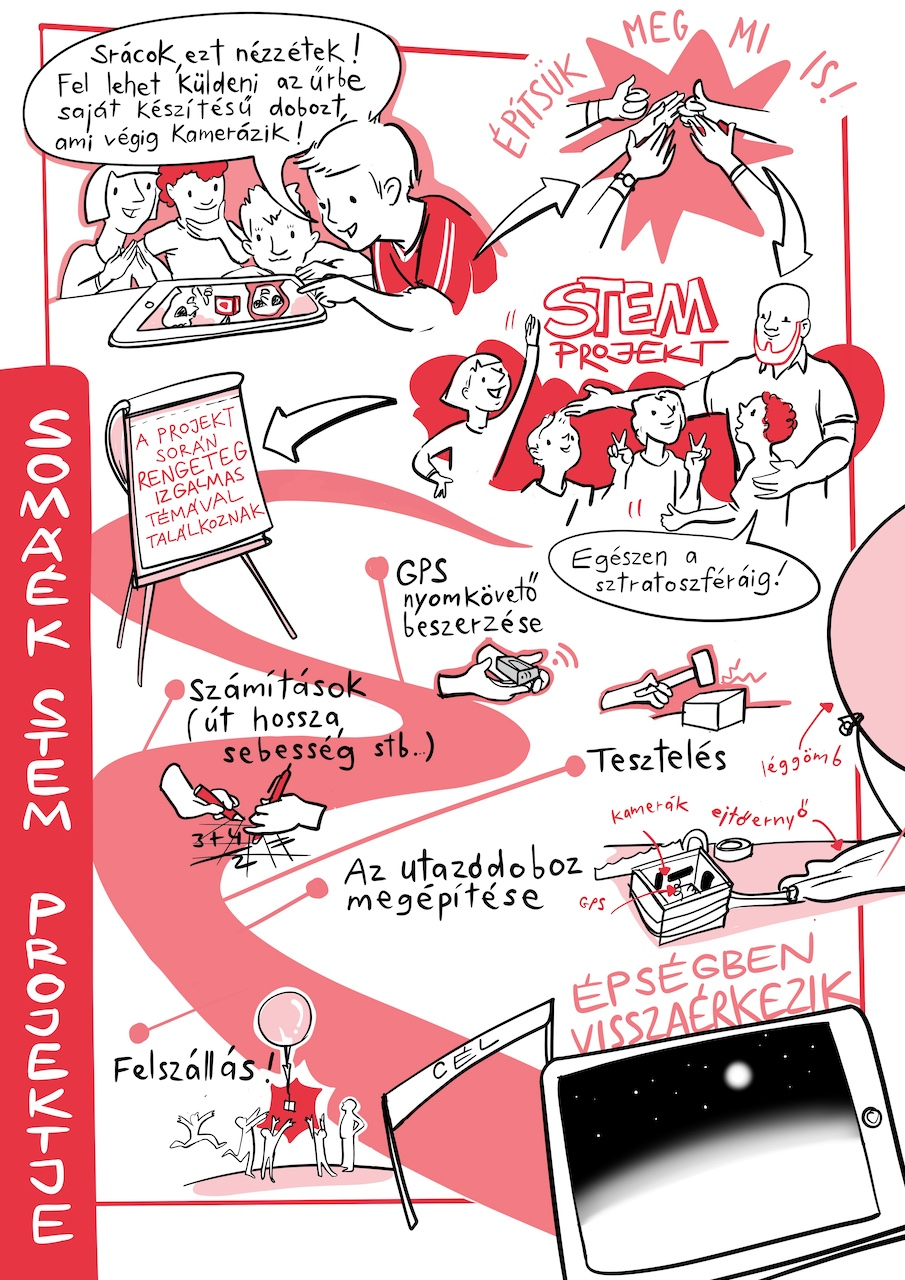
\includegraphics{pics/2a_stem.jpg}
\caption{A STEM a felfedezés és megismerés vágyát tartja ébren.}
\end{figure}

\hypertarget{stem-fejlesztesi-celok}{%
\paragraph{STEM fejlesztési célok}\label{stem-fejlesztesi-celok}}

\begin{itemize}
\tightlist
\item
  Problémamegoldási képesség fejlesztése
\item
  Matematikai gondolkodás fejlesztése
\item
  Logikus gondolkodás fejlesztése
\item
  A világ működésének mélyebb megértése a természettudományos
  szemléleten keresztül
\item
  Innovatív fejlesztésekhez szükséges technológiai (kódolás) és
  gyakorlati (maker) eszköztár megismerése és alkalmazása
\end{itemize}

A STEM komplex, tudományterületeken és a technológiai lehetőségeken
átívelő megközelítése sokfelé ágazik, mégis vannak olyan alapszabályai,
amelyek a tanulás során mindig jellemzik. Ahhoz, hogy folyamatos
fejlődés legyen, fontos, hogy a tanulás az aktuális képességekhez igazodó,
nyitott, tényeken alapuló, kutatásalapú, diverz módszertanú,
skálázható legyen,
és releváns módon történjen a STEM területen.

A STEM terület a fenti célok eléréséhez a következő egymást segítő
komponensek alkalmazását javasolja:

\hypertarget{gyakorlatias-tanulas-elkotelezett-es-egyuttmukodo-kozossegek-halozatahoz-kapcsolodva}{%
\paragraph{Gyakorlatias tanulás elkötelezett és együttműködő közösségek
hálózatához
kapcsolódva}\label{gyakorlatias-tanulas-elkotelezett-es-egyuttmukodo-kozossegek-halozatahoz-kapcsolodva}}

A STEM-tanulás során különösen fontos, hogy az adott területet jól
ismerő szaktanár és a mentoron túl további innovatív és segítő közegek
is támogassák a gyerekek fejlődését. Sokat hozzátehet a mindennapi
élethez való kapcsolódás kialakításában, ha intézményi (pl. múzeum,
kutatóintézet) vagy technológiai, ipari és más STEM-hez kapcsolódó
területen működő cégeknél dolgozó emberek mintákat mutatnak, vagy akár
bekapcsolódnak a gyerekek mindennapos munkájába.

\hypertarget{hozzaferheto-tanulasi-gyakorlatok-amelyek-a-jatek-es-a-kockaztatas-eszkozeit-is-felhasznaljak}{%
\paragraph{Hozzáférhető tanulási gyakorlatok, amelyek a játék és a
kockáztatás eszközeit is
felhasználják}\label{hozzaferheto-tanulasi-gyakorlatok-amelyek-a-jatek-es-a-kockaztatas-eszkozeit-is-felhasznaljak}}

A STEM tematikájú játékok segítik a gyerekeket abban, hogy egymástól és
együtt is tanuljanak, ezzel fejlesztik a kreativitásukat és a felfedezés
iránti vágyukat. Ezek a felfedeztető játékok ráirányítják a fókuszt a
csapatmunka fontosságára, és arra, hogy miként lehet mai problémákra és
kihívásokra válaszokat találni.

\hypertarget{multidiszciplinaris-tanulasi-elmenyek-amelyek-a-vilag-nagy-kihivasaira-keresnek-valaszokat}{%
\paragraph{Multidiszciplináris tanulási élmények, amelyek a világ nagy
kihívásaira keresnek
válaszokat}\label{multidiszciplinaris-tanulasi-elmenyek-amelyek-a-vilag-nagy-kihivasaira-keresnek-valaszokat}}

A STEM legfőbb kihívása, hogy a mai kor olyan kérdésfelvetéseit
vizsgálja, amelyekre közösségi, nemzeti vagy globális\break
szinten még
nincsenek meg a válaszok. Ezek lehetnek a vízgazdálkodással, az
agykutatással és annak a prevencióra, vagy épp a gyógyulásra gyakorolt
hatásaival, a megújuló energiagazdálkodással, vagy épp az önvezető autók
új generációjának technológiai irányaival kapcsolatosak.

Ezek a kihívások egyúttal azt is megmutatják, hogy mely kérdések
lehetnek a kultúránk szempontjából relevánsak.

\hypertarget{rugalmas-es-nyitott-tanulasi-kornyezet}{%
\paragraph{Rugalmas és nyitott tanulási
környezet}\label{rugalmas-es-nyitott-tanulasi-kornyezet}}

A STEM élményszerű tanulásához nagyban hozzájárulhatnak a nyitottan
értelmezett tanulási környezetek. Az iskolai terek alkotótérré
változtatásával, a természeti közegekben végzett terepmunkák vagy a
korszerű technológiai platformok, mint például a VR (virtuális valóság
-- virtual reality) vagy AR (kiterjesztett virtuális valóság --
augmented virtual reality) bevonásával a területek könnyebben
megismerhetővé válnak, és újabb kérdések feltevésére sarkallhatják a
gyerekeket, miközben az irányító tanárszerep helyett a kísérletező,
segítő és facilitátor feladatok erősödnek.

\hypertarget{a-tanulasi-eredmenyek-meresenek-uj-eszkoztara}{%
\paragraph{A tanulási eredmények mérésének új
eszköztára}\label{a-tanulasi-eredmenyek-meresenek-uj-eszkoztara}}

A teljesítmény, a kutatás, a kísérletezés és az alkotás kiemelt fókuszú
a gyerekek STEM tanulási útja során. Kiemelt szerepet kapnak ezért a
saját kutatásokra épülő prezentációk, megfigyelések és az azokra adott
értékes visszajelzések.

\hypertarget{kultura-tarsadalom-kommunikacio-es-muveszetek-kult}{%
\subsection{Kultúra, társadalom, kommunikáció és művészetek
(KULT)}\label{kultura-tarsadalom-kommunikacio-es-muveszetek-kult}}

A művészetek és önmagunk kifejezése az őskortól segítik az embereket a
túlélésben. A képzelet absztrakciós szintjének alkalmazása az egyik
legfontosabb faji tulajdonsága az embernek. Ennek fejlesztése pedig
globális világunk egyik legnagyobb kihívása. Ahhoz, hogy a társadalmi
viták és szabályozások aktív alakítójává válhassunk, hogy megismerjük a
globális világunk legnagyobb kihívásait, értenünk kell a múltunkat, a
saját kultúránkat és a kultúrák szerepét általában, és ki kell tudnunk
fejezni magunkat olykor szavakkal, máskor a művészet eszközeivel.

Még soha nem élt az emberiség ennyire behálózott világban, és még soha
nem kellett ennyire tudatosan készülnünk arra, hogy gyerekeinknek
többféle kultúrát, társadalmi hálózatot kell megérteniük, és abban
eligazodniuk. Családok, munkahelyi és lakókörnyezeteink, sőt még a
nemzeti és az azokat átívelő társadalmi környezetek is gyorsabban
változnak ma, mint szüleink életében. Ezért szeretnénk, hogy gyerekeink
stabil identitásukra építkezve képesek legyenek emberként emberekhez
kapcsolódni, embertársaikat megérteni, velük együtt élni, dolgozni.

\begin{figure}
\centering

\includegraphics{pics/2b_kult.jpg}
\caption{A KULT fejleszti az empátiát, kommunikációt, önkifejezést, kapcsolódást.}
\end{figure}

A tanulás egyik legfőbb funkciója, hogy képessé váljunk egy fenntartható
élet kialakítására. Ehhez pedig önmagunk, környezetünk (Harmónia) és a
világ működésének megismerésén (STEM) és fejlesztésén túl a szűk és
tágabb értelemben vett kulturális tereinkhez is kapcsolódnunk kell
(KULT). Meg kell ismernünk a lokális és a globális kihívásokat ahhoz,
hogy értő, empatikus módon kapcsolódhassunk a saját és más kultúrákhoz,
és a fenntartható fejlődés alakítójává válhassunk. A Budapest \mbox{School}
KULT terület fő célja ezért az olyan globális kompetenciák fejlesztése,
amelyek a fenti cél elérését támogatják.

A KULT terület a következő fejlesztési területeket foglalja magába:

\begin{itemize}
\tightlist
\item
  írott és beszélt anyanyelvi kommunikáció
\item
  írott és beszélt idegen nyelvi kommunikáció
\item
  mai lokális és globális kihívások megismerése a múlt kontextusában
\item
  kulturális diverzitás és a kultúra mint az emberi viselkedést leíró
  eszköztár megismerése
\item
  művészetek stílus- és formavilága
\item
  művészetek mint önkifejezési eszköz a vizuális (hagyományos
  képzőművészetektől a digitális művészetekig) és előadóművészetekben
  (dráma, tánc, zene)
\end{itemize}

Miközben világunkban egyre nő a technológia szerepe, folyamatosan nő az
igény arra is, hogy képesek legyünk értelmezni és megfelelően használni
az elénk táruló információt. Ennek alapja a megfelelő szövegértés, a
nyelvnek mint írott és verbális kommunikációs stratégiának az egyéni és
korosztályi képességekhez mért alkalmazása, valamint a művészeteken
keresztül a kifejezés egyéb módjainak elsajátítása. Ahhoz, hogy képessé
váljunk erre, megfelelő történelmi és kulturális kontextusba kell
helyeznünk az elénk táruló információt, és nyitottnak kell lennünk arra,
hogy ezeket befogadjuk, és a mai kor globális kihívásaihoz képest
értelmezhessük.

A KULT komplex tanulási struktúrája adja meg az új információk
elmélyülésének alapjait, és segít abban, hogy a mindennapos döntési
stratégiáink részévé váljanak.

A KULT az alábbi képességeket fejleszti:
\newpage
\begin{itemize}
\tightlist
\item
  Empátia és együttérzés
\item
  Egyéni és közösségi hiedelmek felismerése
\item
  Mérlegelő gondolkodás
\item
  A művészetek és az irodalom funkciójának felismerése és a mindennapi
  életbe való beépítése
\item
  Az etika és a morál alapkérdéseinek felfedezése és megkérdőjelezése
\item
  Új ötletek befogadása
\item
  Az emberiség kulturális örökségének és aktuális diverzitásának
  kiaknázása
\item
  Többsíkú gondolkodás, multidiszciplináris szövegértés
\end{itemize}

A KULT terület a fenti célok eléréséhez a következő egymást segítő
komponensek alkalmazását javasolja:

\hypertarget{helyi-kozossegekhez-valo-kapcsolodas}{%
\paragraph{Helyi közösségekhez való
kapcsolódás}\label{helyi-kozossegekhez-valo-kapcsolodas}}

Tanulás során a lokális közösségek szerepe megnő, hiszen mind a saját
kultúra és művészeti értékek megismerése, mind a nyelvhasználat
tekintetében döntő szerepe van annak, hogy saját környezetünkben tudjuk
ezeket érteni és alkalmazni.

\hypertarget{kortars-kihivasok}{%
\paragraph{Kortárs kihívások}\label{kortars-kihivasok}}

A KULT alapját a kortárs művészeti értékek, a kortárs problémák és
kihívások adják. Ezek ugyan mindig a múlt és a környezet kontextusában
értelmezhetők, de elsődleges módszer a kapcsolat kialakítása a mai világ
alkotásaival, szövegeivel, kulturális értékeivel.

A KULT abban segít a gyerekeknek, hogy jobban eligazodjanak a mai és
holnapi világban, és olyan kérdéseket tegyenek fel, amelyek ma még
megválaszolatlanok, és a jövőt formálhatják. Ehhez a művészetek, nyelvek
és kultúrák találkozási pontjait, az átmeneteket is célszerű szemlélni.

\hypertarget{rugalmas-es-befogado-tanulasi-kornyezet}{%
\paragraph{Rugalmas és befogadó tanulási
környezet}\label{rugalmas-es-befogado-tanulasi-kornyezet}}

A mai szövegek értelmezése, az online elérhető tartalmakban való
tájékozódás képessége éppoly fontos, mint az idegen nyelveken történő
kommunikáció elősegítése a világhoz történő kapcsolódással. Az aktuális
globális kihívásokat a múltunkon keresztül érthetjük meg, amihez
tanulási környezetünket folyamatosan a megismerés igényeihez képest kell
formálnunk, és olyan eszközöket kell használnunk, amelyek az értelmezést
segíthetik.

\hypertarget{alkotoi-szabadsag-es-az-alkoto-szabad-ertelmezese}{%
\paragraph{Alkotói szabadság és az alkotó szabad
értelmezése}\label{alkotoi-szabadsag-es-az-alkoto-szabad-ertelmezese}}

Az önálló alkotói munka és az alkotások szabad értelmezése és befogadása
az innováció és a kreativitás alapja. Ennek biztosításához a hagyományos
keretek újraértelmezésére van szükség és arra, hogy egy alkotói
folyamatban a saját cél kibontakozásának támogatása megtörténjen.

\hypertarget{harmonia-fizikai-lelki-jollet-es-kapcsolodas-a-kornyezethez}{%
\subsection{Harmónia (fizikai, lelki jóllét és kapcsolódás a
környezethez)}\label{harmonia-fizikai-lelki-jollet-es-kapcsolodas-a-kornyezethez}}

Testi és lelki egészségünk az alapja annak, hogy tanulhassunk,
fejlődhessünk, és a saját életünk alakítóivá váljunk. Életünk fizikai,
lelki, érzelmi és társas aspektusai határozzák meg a kapcsolódásunkat
önmagunkhoz, társainkhoz és az őket körülvevő emberekhez, vagyis a
tágabb értelemben vett társadalomhoz. Ez segít abban, hogy önálló
döntéseket hozzunk, és jól tudjunk együtt tanulni, dolgozni
csoportokban. Ahhoz, hogy a közösségünk részeként harmóniában élhessünk
önmagunkkal, az épített és természeti környezetünkhöz is kapcsolódnunk
kell.

A Budapest School tanulási koncepciójának középpontjában az egyén, mint
a közösség jól funkcionáló, saját célokkal rendelkező tagja áll. Az
iskolában való fejlődése során elsősorban azt tanulja, hogy miként tud
specifikált saját célokat megfogalmazni, és hogyan tudja ezeket elérni.
Ebben a folyamatban egy mentor segíti a munkáját az iskola kezdetétől a
végéig. Ő figyel arra, hogy a gyerek fizikai és lelki biztonsága és
fejlődése folyamatos legyen, és segíti azokban a helyzetekben, amikor
biztonságérzete vagy stabilitása csökken.

A közösségben jól funkcionáló egyén belső harmóniájához a következő
fejlesztési területeket tartja az iskola fontosnak:

\begin{itemize}
\tightlist
\item
  Érzelmi és társas intelligencia
\item
  Önismeret és önbizalom
\item
  Konfliktuskezelés
\item
  A nehéz élethelyzetekkel történő megküzdés készségei (reziliencia)
\item
  Mérlegelő gondolkodás
\item
  Közösségi szabályok alkotásában való részvétel és azok alkalmazása
\item
  Csapatmunka gyakorlati fejlesztése
\item
  Oldott játék
\item
  Egészséges testi fejlődés
\item
  Saját igényekhez képest megfelelő táplálkozás
\item
  A természettel való kapcsolódás
\item
  Épített falusi és városi környezetben való eligazodás
\item
  A technológia világában felhasználói szintű eligazodás és annak\break
  harmonikus alkalmazása
\end{itemize}

A Harmónia a fenti célok eléréséhez a következő egymást segítő
komponensek alkalmazását javasolja:

\vspace*{-1ex}
\hypertarget{kozossegben-csapatban}{%
\paragraph{Közösségben, csapatban}\label{kozossegben-csapatban}}

A Budapest School egy közösségi iskola, ahol a közösség tagjai egymással
és egymástól tanulnak. A közösségekhez való tartozáshoz, a csapatban
való gondolkodáshoz, és a családban való működéshez szükséges
képességeket leginkább úgy tudjuk fejleszteni, ha azt a kezdetektől
megéljük. A közösség belső szabályainak megalkotása és az azokhoz való
kapcsolódás a tanulás folyamatosságának alapfeltétele.

\vspace*{-1ex}
\hypertarget{eletkepessegek-life-skills}{%
\paragraph{Életképességek (life
skills)}\label{eletkepessegek-life-skills}}

Szeretnénk, ha gyerekeink általában alkalmazkodóan (adaptívan) és
pozitívan tudnának hozzáállni az élet kihívásaihoz, ha lelki és fizikai
erősségük és ellenálló képességük (rezilienciájuk) megmaradna és
fejlődne. A Egészségügyi Világszervezet {\autocite{WHO1999}} a
következőképpen definiálta az életképességeket:

\begin{itemize}
\tightlist
\item
  Döntéshozás, problémamegoldás
\item
  Kreatív gondolkodás
\item
  Kommunikáció és interperszonális képességek
\item
  Önismeret, empátia
\item
  Magabiztosság (asszertivitás) és higgadtság
\item
  Terhelhetőség és érzelmek kezelése, stressztűrés
\end{itemize}

\vspace*{-1ex}
\hypertarget{erzelmi-intelligencia}{%
\paragraph{Érzelmi intelligencia}\label{erzelmi-intelligencia}}

Sokszor kiemeljük az érzelmi intelligenciát, hangsúlyozva, hogy
gyerekeinknek többet kell foglalkozniuk az érzelmek felismerésével,
kontrollálásával és kifejezésével, mint szüleiknek kellett.

\vspace*{-1ex}
\hypertarget{szabad-mozgas-es-seta}{%
\paragraph{Szabad mozgás és séta}\label{szabad-mozgas-es-seta}}

A különböző mozgásformák, a sportok és a séta mindennapivá tétele
természetes módon, a gyerekek saját igényei szerint kell, hogy történjen.

\vspace*{-1ex}
\hypertarget{gyakorlatias-mindennapi-kepessegek}{%
\paragraph{Gyakorlatias, mindennapi
képességek}\label{gyakorlatias-mindennapi-kepessegek}}

Ahhoz, hogy gyerekeink önállóan és hatékonyan tudják élni életüket, hogy
a társakhoz való kapcsolódás ne függőség legyen, egy csomó praktikus
mindennapi tudást el kell sajátítaniuk. A gyerekeknek folyamatosan
fejleszteniük kell az élethez szükséges mindennapi tudást a
levélszemét-kezeléstől az internet és a szociális média tudatos
használatán át egészen a személyi költségvetés elkészítéséig.

\vspace*{-1ex}
\hypertarget{egeszseges-taplalkozas}{%
\paragraph{Egészséges táplálkozás}\label{egeszseges-taplalkozas}}

Az egészséges táplálkozás tanulható viselkedésforma, melynek alapja
nemcsak a megfelelő élelmiszerek kiválasztása, hanem azok élettani
hatásainak megismerése és az étkezési szokások alakítása is.

\hypertarget{ut-az-eselyegyenloseg-fele}{%
\section{Út az esélyegyenlőség felé}\label{ut-az-eselyegyenloseg-fele}}

A Budapest School lehetőséget kíván biztosítani arra, hogy a a
társadalom minél szélesebb rétegeiből kerülhessenek be gyerekek, hogy a
családok társadalmi, gazdasági státuszától függetlenül, kizárólag saját
fejlődési útjuk kiteljesedése jegyében válhassanak a közösség részévé.

Tudjuk, hogy az esélyek sosem egyenlőek, tenni viszont lehet azért, hogy
minél kiegyenlítettebbek legyenek. A következő területeken a családok
kiválasztásakor és az iskolába járó gyerekekkel való partneri
kapcsolatban azon dolgozunk, hogy senki se érezhesse magát hátrányosan
megkülönböztetve testi, szellemi, kulturális, szociális, nemi vagy
hitbéli egyediségei miatt.

\hypertarget{a-tarsadalmi-statuszban}{%
\paragraph{A társadalmi státuszban}\label{a-tarsadalmi-statuszban}}

A Budapest Schoolba járó családok legalább 30\%-a kevesebb hozzájárulást
fizet, mint amennyi az iskola működésének teljes bekerülési költsége. Az
ő számuk, az általuk fizetendő hozzájárulás mértéke a támogató
családoktól függ. Minél érzékenyebb, minél nagyvonalúbb egy közösség
azok irányába, akik nem tehetik meg, hogy a gyerekük tanulásáért
kifizessék az ahhoz szükséges költségeket, annál nagyobb mértékű a
társadalmi státuszbéli esélyegyenlőség egy adott Budapest School
tanulóközösségben.

\hypertarget{a-nemek-aranyaban}{%
\paragraph{A nemek arányában}\label{a-nemek-aranyaban}}

A Budapest School tanulóközösségeiben a nemek arányának
kiegyenlítésére törekszünk. Folyamatosan monitorozzuk a fiúk és lányok arányát az egyes
közösségekben, és ha az elcsúszik valamely irányba, akkor a
felvételi során a kiegyenlítés irányába hozunk döntéseket.

\hypertarget{a-kulturalis-es-vallasi-egyedisegekben}{%
\paragraph{A kulturális és vallási
egyediségekben}\label{a-kulturalis-es-vallasi-egyedisegekben}}

A BPS-iskolában meghatározó, észrevehető a családok értékrendje, mert a
családok részei a közösségnek. A családok pedig jöhetnek azonos, de
jöhetnek diverz kulturális és vallási környezetből is. Az ő szempontjaik
tiszteletben tartása mindaddig kiemelten fontos, amíg az nem
veszélyezteti a közösségben együtt tanuló gyerekek fejlődését.

\hypertarget{a-fejlodes-sebessegeben}{%
\paragraph{A fejlődés sebességében}\label{a-fejlodes-sebessegeben}}

A Budapest School lehetőséget biztosít arra, hogy a gyerek a saját
tempójában, a saját maga által kijelölt és komfortos tanulási úton
haladjon addig, amíg ebben a mentortanárával és a szüleivel is közös
megállapodást kötnek. A fejlődés sebessége azonban nem akadályozhatja a
közösségben tanulást. A tanulásszervezők felelőssége annak
meghatározása, hogy a közösségben lassabban fejlődő gyerekek
mennyiben veszélyeztetik, vagy mennyiben segítik a tanulásszervezést a
közösség egésze szempontjából.

\hypertarget{a-tanulas-tartalmaban}{%
\paragraph{A tanulás tartalmában}\label{a-tanulas-tartalmaban}}

A BPS-iskolában minden gyereknek van saját\break
célja. Ennek hossza,
komplexitása minden esetben egyedi, függ a gyerek érdeklődésétől,
érettségétől, családi helyzetétől, mentális és fizikai állapotától. A
tanulás tartalmában mindenkinek van lehetősége arra, hogy a maga útját
járja, ha figyelembe veszi, hogy ezt a közösség részeként kell tennie.

\hypertarget{a-testi-es-szellemi-egyedisegben}{%
\paragraph{A testi és szellemi
egyediségben}\label{a-testi-es-szellemi-egyedisegben}}

A Budapest School tanulóközösségeiben a tanulásszervezők felelőssége
annak eldöntése, hogy egy adott közösség milyen mértékben tud befogadni
sérült vagy sajátos nevelési igényű gyerekeket. Az ő befogadásukkor és a
velük való kiemelt foglalkozáskor mindig arra a kérdésre kell
válaszolni, hogy tudjuk-e garantálni a gyerek fejlődését, elég
biztonságos-e a közeg a számára, és az iskolában való szerepe miként
segíti a többi gyerek fejlődését.

\hypertarget{a-donteshozasban}{%
\paragraph{A döntéshozásban}\label{a-donteshozasban}}

A Budapest School-döntéshozatal nem többségi és nem konszenzusos
megállapodások alapján történik. A döntések esélyt adnak arra, hogy
minden kellően biztonságos, elég jó javaslatot ki lehessen próbálni
akkor, ha az nem áll szemben a közösen elfogadott célokkal, és nem sérti
bármely egyén érdekeit olyan mértékben, ami sérti a biztonságérzetét.

\hypertarget{a-kiemelt-figyelmet-igenylo-gyerekek}{%
\section{A kiemelt figyelmet igénylő
gyerekek}\label{a-kiemelt-figyelmet-igenylo-gyerekek}}

A kiemelt figyelmet igénylő gyerekek támogatásához elsődlegesen a
tanulásszervezőknek, a mentoroknak és a szaktanároknak kell
differenciáltan, sokszínűen, türelemmel és személyre szabottan
foglalkozni.

\begin{itemize}
\tightlist
\item
  A mentoroknak ismerniük kell a gyerek sajátosságait. A szülőnek és a
  mentornak őszintén, egymást segítve kell a gyerek egyéni támogatására
  felkészülniük. Ehhez sokszor külső diagnózisra, szakember bevonására és
  a felnőttek közötti nehéz beszélgetésekre van szükség.
\item
  A mentoroknak meg kell osztaniuk a gyerekek sajátos igényeit a többi
  tanárral, a szaktanárokkal, hogy ők is fel tudjanak készülni a
  gyerekek személyre szabott támogatására.
\item
  A tanulásszervezésnek, a moduloknak, a foglalkozásoknak, azaz a
  gyerekek teljes tanulási élményének differenciáltnak, egyéniesítettnek
  kell lennie, hogy az eltérő képességekkel bíró gyerekek is tudjanak
  együtt tanulni. Ahogy egy nagycsaládban is figyelünk a különböző
  gyerekek eltérő igényeire, képességszintjeire.
\item
  A szemléltetésnek, a tevékenységeknek sokoldalúaknak kell lenniük,
  sokféle feladatot, speciális eszközöket kell használni. A gyerekek
  élménye változatos kell, hogy legyen.
\item
  Külső szakemberekkel kell konzultálni, és a diagnózisban szereplő
  javaslatokat be kell építeni a mindennapok tervezésébe. Ebben a
  szülőnek és a tanároknak szorosan együtt kell működniük.
\item
  Az egyéni haladási ütem biztosítására egyéni fejlesztési és tanulási
  tervet kell készíteni.
\item
  A tanároknak együtt kell működniük a gyermek/tanuló fejlesztésében
  részt vevő szakemberekkel.
\end{itemize}

A fenti listából a legfontosabb elem: a tanár---gyerek---szülő hármas
mellé be kell általában hívni külső, a gyerek igényeit jól értő
szakembert támogatónak. A Budapest School-iskola csak akkor tud
segíteni, ha minden fél tudatosan áll hozzá a kiemelt figyelem
szükségletéhez.

\chapter{A tanulási élmény}
\hypertarget{a-szemelyre-szabhato-kozossegi-iskola}{%
\section{A személyre szabható közösségi
iskola}\label{a-szemelyre-szabhato-kozossegi-iskola}}

Az iskola több helyszínen működik. A gyerekek az iskolában kisebb
közösségekbe tartoznak, a
tanulóközösségekbe (\ref{a-budapest-school-tanulokozossegei}.~fejezet, \pageref{a-budapest-school-tanulokozossegei}.~oldal).
Ezek a közösségek legfeljebb hat évfolyamot átölelő, 6-60 fős tanulási
közösségekként működnek. A tanulóközösségek se jogi, se szervezeti
szempontból nem önálló iskolák, nem összevont osztályok. A
tanulóközösség nem más, mint az iskola egyik szervezeti egysége, ami
önálló identitással, sajátos szubkultúrával, szabályokkal rendelkezhet.

A kisközösségükön belül a gyerekek többfajta csoportbontásban tanulnak,
és idősebb korban (10-12 év felett) különböző osztályok, közösségek
tagjai is összeállhatnak egy-egy foglalkozásra, kurzusra, de
identitásban, ,,egymáshoztartozás-érzésben'' a tanulóközösség az
elsődleges közösségük. A közösség tagjai együtt és egymástól tanulnak.

Az egyes tanulóközösségeket
tanulásszervező tanárok (tanulásszervezők, \ref{tanulasszervezo}.~fejezet, \pageref{tanulasszervezo}.~oldal)
csapata vezeti. Minden gyereknek van egy kitüntetett tanára, a
mentora (\ref{mentor}.~fejezet, \pageref{mentor}.~oldal), aki egyéni
figyelmével a fejlődésben segíti. Minden gyerek a mentortanára
segítségével és a szülők aktív részvételével trimeszterenként
meghatározza a
saját tanulási céljait (\ref{sajat-tanulasi-celok}.~fejezet, \pageref{sajat-tanulasi-celok}.~oldal).

A tanulásszervezők
modulokat (\ref{tanulasi-tanitasi-egysegek-a-modulok}.~fejezet, \pageref{tanulasi-tanitasi-egysegek-a-modulok}.~oldal)
hirdetnek ezen célokból és a tantárgyak tanulási eredmények alapján. A
modulok reflektálnak a mai világ alapvető kérdéseire, integrálják a
tudományterületeket és művészeti ágakat, azaz a tantárgyakat, és egyenlő
lehetőséget adnak a tudásszerzésre, az önálló gondolkodásra és az
alkotásra a gyerekek mindennapjaiban.

A modulok végeztével a gyerekek eredményei bekerülnek saját
portfóliójukba (\ref{portfolio}.~fejezet, \pageref{portfolio}.~oldal),
ami tartalmazhat önálló vagy csoportos alkotásokat, tudáspróbákat,
vizsgafeladatokat, egymás felé történő visszajelzéseket, a fejlődést jól
mérő dokumentációkat vagy bármit, amire a gyerek és tanárai büszkék, vagy
amit fontosnak tartanak. Erre a portfólióra épül a Budapest School
visszajelző és értékelő rendszere (\ref{visszajelzes-ertekeles}.~fejezet, \pageref{visszajelzes-ertekeles}.~oldal).

A gyerekek mindennapjait meghatározó modulok több műveltségi területet,
többféle kompetenciát, több tantárgy anyagát is lefedhetik, és egy
tantárgy anyagát több modul is érintheti. Ezért is mondhatjuk, hogy a
BPS-iskolákban a tantárgyközi tevékenységek vannak előtérben. Az iskola
szándéka, hogy a gyerekek folyamatosan fejlődjenek a világ tudományos
megismerésében (STEM), a saját és mások kulturális közegéhez való
kapcsolódásban (KULT), valamint a testi-lelki egyensúlyuk fenntartásában
(Harmónia), vagyis a
kiemelt tantárgyközi fejlesztési területeken (\ref{kiemelt-fejlesztesi-teruletek}.~fejezet, \pageref{kiemelt-fejlesztesi-teruletek}.~oldal).

Az iskola szerint az a tanárok döntése, hogy a gyerekek kémiaórán
kísérleteznek-e, vagy kísérletezésórán foglalkoznak kémiával. A iskola\break
annyit határoz meg, hogy a 7--10. évfolyamszinten kémia tantárgyhoz
kapcsolódóan 73 különböző tanulási eredményt kell elérni,
kísérletezéssel\break
kapcsolatban pedig 21 különböző tanulási eredményt több
különböző tantárgyból (ezekből csak 8 kapcsolódik a kémia tantárgyhoz).

Tehát a tantárgyak a tanulás tartalmi elemeinek forrásai és keretei: a
tanulandó dolgok halmazaként működnek. Az, hogy milyen csoportosításban
történik a tanulás, a szaktanárokra van bízva. A gyerekek lehet, hogy
csak félévente, az elszámolás időszakában találkoznak a tantárgyak
taxonómiájával. Ebben az időszakban veti össze minden gyerek és mentor,
hogy amit tanultak, alkottak, és amiben fejlődtek, az hogyan viszonyul a
társadalom és a törvények elvárásaihoz, a Nemzeti Alaptantervhez.

Az iskola a NAT-tantárgyak témaköreit, tartalmát és követelményeit
\emph{tanulási eredmények} halmazaként adja meg. A gyerekek feladata az
iskolában, hogy tanulási eredményeket érjenek el, és így sajátítsák el a
tantárgyak által szabott követelményeket. Tanulási eredményeket modulok
elvégzésével (is) el lehet érni, tehát a modulok elsődleges feladata,
hogy a tanulási eredményekhez vezető utat mutassák.

Az iskolában egyszerre jelennek meg a NAT tantárgyi elvárásai, a
közoktatást szabályozó törvények szándékai, a gyerekek saját céljai és a
mai világra való integrált reflexió.

\hypertarget{a-tanulas-rendszerszemleletu-megkozelitese}{%
\subsection{A tanulás rendszerszemléletű
megközelítése}\label{a-tanulas-rendszerszemleletu-megkozelitese}}

Az oktatás tartalmának előzetes szabályozása helyett a Budapest School a
tanulás módjára helyezi a hangsúlyt. Az iskola alapelve, hogy integratív
módon folyamatosan keresse és fejlessze a pedagógiai, pszichológiai és
szervezetfejlesztési módszereket, amelyek korszerű módon tudják segíteni
a tanulás tanulását, az egyéni és csoportos fejlődést, a konfliktusok
feloldását.

A tanulás tartalmát tekintve a Budapest School a NAT tartalmára
támaszkodik. A Budapest School Modell pedig a tanulás rendszerét, annak
folyamatát szabályozza. E dokumentum alapján a NAT tanulási eredményein
történő végighaladás mellett a Budapest School nagy hangsúlyt fektet a
gyerekek saját tanulási céljaira és a célállítás módjára.

\hypertarget{sajat-tanulasi-celok}{%
\section{Saját tanulási célok}\label{sajat-tanulasi-celok}}

Minden gyerek megfogalmazza és háromhavonta újrafogalmazza a \emph{saját
tanulási céljait}: eredményeket, amelyeket el akar érni, képességeket,
amelyeket fejleszteni akar, szokásokat, amelyeket ki akar alakítani. A
saját célok elfogadásakor a gyerek és a mentora a szülőkkel együtt
\emph{tanulási szerződést} köt.

Csak olyan célok kerülhetnek a saját célok közé, amelyek minden
érintettnek biztonságosak. Annyi megkötés van, hogy céloknak mindenképp
ki kell terjedniük a tantárgyi tanulási eredményekre (\emph{,,mennyit és
hogyan akarok elérni a NAT-ból származó tanulási eredményekből''}) és a
tantárgyi rendszeren kívüli célokra, feladatokra is.

Háromhavonta a tanulásszervezők és a gyerekek megállnak, reflektálnak az
elmúlt időszakra, és a tapasztalatok, valamint az elért célok
ismeretében és az új célok figyelembevételével újraszervezik a
foglalkozások rendjét, tehát azt, hogy mikor és mit csinálnak majd a
gyerekek az iskolában. A mindennapi tevékenység során tapasztalt
élmények, alkotások, elvégzett feladatok és vizsgák, tehát
mindaz, ami a gyerekekkel történik, bekerül a portfóliójukba. Még az is,
amit nem terveztek meg előre.

A gyerekeket a mentoruk segíti a saját célok kitűzésében, a különböző
választásoknál, a portfólióépítésben, a reflektálásban. A tanulási célok
kitűzése az önirányított tanulás fokozatos fejlődésével és az életkor
előrehaladtával folyamatosan egyre önállóbb tevékenységgé válik.
Tanulási útjukon, céljaik kitűzésében a mentor kíséri végig a gyerekeket.

A Budapest School személyre szabott tanulásszervezésének
jellegzetessége, hogy a gyerekek a saját céljuk irányába haladnak, az
adott célhoz az adott kontextusban leghatékonyabb úton. Tehát mindenki
rendelkezik saját célokkal, még akkor is, ha egy közösség tagjainak
céljai a tantárgyi tanulási eredmények azonossága, vagy a hasonló
érdeklődés miatt akár 80\% átfedést mutatnak.

A NAT műveltségi területeiben és a tantárgyakban megfogalmazott
követelmények teljesítése is célja a tanulásnak, a tanulás fő irányítója
azonban más. Mi azt kérdezzük a gyerekektől, hogy \emph{ezen felül} mi
az ő személyes céljuk.

\hypertarget{mentoralas}{%
\section{Mentorálás}\label{mentoralas}}

Minden gyereknek van egy \emph{mentora}, aki a saját céljainak
megfogalmazásában és a fejlődése követésében segíti. A mentor segít az
általa mentorált gyereknek, hogy a tantárgyi fejlesztési célok és a
saját magának megfogalmazott saját célok között megtalálja az
egyensúlyt, és segít megalkotni a gyerek \emph{saját tanulási tervét}.

Minden gyerek rendszeresen találkozik a mentorával, hogy átbeszéljék, hol
is tart a gyerek a céljai elérésében, milyen lehetőségei, döntései
és tervei vannak. A mentor feladata segíteni a gyereket
felismerni céljait, lehetőségeit és megtalálni a saját válaszait. A
kapcsolat lényege, hogy intim, közvetlen, őszinte, gyerekfókuszú és
rendszeres.

\hypertarget{mentorido}{%
\subsection{Mentoridő}\label{mentorido}}

Minden gyerek egy órát hetente a mentorával tölt, amikor a mentor a
gyerek számára egyéni, minőségi figyelmet ad. A mentor ilyenkor a
gyereket segíti a saját céljainak megfogalmazásában és hogy legyen
lehetősége reflektálni a saját fejlődésére. Ez az óra a gyerekek és a
mentorok számára kötelező foglalkozás.

\hypertarget{mentornaplo}{%
\subsection{Mentornapló}\label{mentornaplo}}

Minden gyereknek van egy mentornaplója, amibe mentorként minden
mentortalálkozó esetén érdemes jegyzeteket készíteni arról, hogy mit
beszélt meg a mentorált és a mentor. Ezekhez sorvezetőként a következő
kérdéseket javasoljuk:

\begin{itemize}
\tightlist
\item
  Mi \emph{van} most? Hogy van a mentorált, mi foglalkoztatja
  mostanában. Mi az, amiről mindenképpen kell ma beszélni?
\item
  Mi \emph{volt} az elmúlt időszakban? Mivel haladt, mit tanult, miyen
  problémái voltak a mentoráltnak? Mi ment jól, mi volt nehézség? Milyen
  tanulságok vannak?
\item
  Mi \emph{lehetne} az új időszakra a cél, miket lehetne megcsinálni,
  kipróbálni, változtatni, folytatni?
\item
  Mi \emph{lesz} ebből a terv? Mi az a 2-3 dolog, amit ezért biztosan
  meg fogsz tenni? Milyen érzések vannak benned ezzel kapcsolatban?
  Kire, mire számíthatsz ebben? Milyen nehézségekre számítasz? Mik azok
  az erőforrásaid, amik már most rendelkezésedre állnak ahhoz, hogy
  ezeken a nehézségeken átlendülj? Hogyan tudok neked én segíteni?
\end{itemize}

Érdemes feljegyezni, hogy milyen kérdések merültek fel, és a mentorált
milyen válaszokat adott magának.

\hypertarget{grow-modell}{%
\subsection{GROW modell}\label{grow-modell}}

Minden mentornak meg kell találnia azokat a kérdéseket, amik ott és
akkor segítik a mentorált fejlődését. Alapjában azt javasoljuk, hogy
minden mentor a GROW modellt szabja magára. A GROW modell egy nagyon
egyszerű és nagyszerű coaching modell. A szó maga azt jelenti:
,,növekedés'', a betűk a következőket jelentik benne:

\begin{itemize}
\tightlist
\item
  \emph{G}oal: \textsc{cél}
\item
  current \emph{R}eality: \textsc{jelenlegi helyzet}
\item
  \emph{O}ptions, \emph{O}bstacles: \textsc{lehetőségek, akadályok}
\item
  \emph{W}ill, \emph{W}ay forward: \textsc{szándék, előre vezető út}
\end{itemize}

A GROW coaching modell használatát a szakirodalom egy utazás\break
megtervezéséhez hasonlítja. Ahhoz, hogy egyáltalán elérj valahová,
tudnod kell, hová akarsz menni (cél), és azt is, hogy hol vagy jelenleg
(jelenlegi helyzet). Aztán az úticél eléréséhez ismerned kell, hogy
hogyan juthatsz oda, mik lehetnek az akadályok, végül pedig el kell
határoznod magad, hogy el is indulsz és legyőzöd ezeket.

\paragraph{G: Célkitűzés.} A mentor segít a gyereknek abban, hogy reális célt tűzzön
ki magának. A célkitűzésben segíthet az, ha a cél SMART cél, tehát
legyen elérhető, reális, időkerethez kötött, mérhető és konkrét.

\paragraph{R: Jelenlegi helyzet meghatározása.} Kritikus pont, hiszen sokszor a
gyerek úgy akar célt kitűzni, hogy nem gondolja át alaposan jelenlegi
helyzetét és azt, így nem rendelkezik a megfelelő mennyiségű
információval ahhoz, hogy reálisan lássa lehetőségeit.

\paragraph{O: Lehetőségek meghatározása.} Ha sikerül az előző lépésben ismertetett helyzetmeghatározás, a
mentor és a gyerek ötletbörzét tarthat a lehetőségekről. A lényeg
megtalálni a lehető legtöbb választási lehetőséget, hogy aztán könnyebb
legyen dönteni, hogy merre induljon a gyerek. Fontos, hogy a mentor
segítse kliensét elszakadni gondolati korlátaitól, segítsen neki
,,messzebbre látni''. Fontos felmérni az akadályokat is.

\paragraph{W: Szándék, elhatározás.} A mentor ebben a szakaszban segít a kliensnek
biztosítani azt, hogy valóban el is induljon a célja felé. A munka
könnyebbik része volt a terep felmérése és a lehetőségek
áttekintése.
Most jön az oroszlánrésze, amikor a kliensnek tennie is kell, méghozzá
nap mint nap azért, hogy el is érje a célját. A mentor feladata a
támogatás, motiválás, inspiráció és a számonkérés is.

\hypertarget{mentor-vagy-coach}{%
\subsection{Mentor vagy coach}\label{mentor-vagy-coach}}

A BPS-mentortanár néha a coach-a, néha mentora a gyereknek. A szakirodalmi
különbség a két fogalom között az, hogy a coach nem ismeri a kliensének
szakterületét, nem ad tanácsot, nem ért jobban a kliensénél a
területhez, ezért tényleg csak abban tud segíteni, hogy a kliens
megtalálja a saját válaszait. Ezzel szemben a mentor az, aki ,,csinálta
már'' (have done it), tapasztalai alapján tanácsokkal tudja ellátni a
mentoráltat. A BPS-mentortanár ebben az értelemben egy tapasztalt,
integráns felnőtt, aki tud segíteni a gyereknek érettebb, önálóbb,
boldogabb felnőtté vállni. Szóval néha tanácsokat ad. A BPS-mentor
ugyanakkor tud coach is lenni. Nem kell ahhoz nagyon érteni az
emeltszíntű biológiához, hogy segíteni tudjunk egy gyereket abban, hogy
ha a céljai úgy kívánják, akkor hetente kétszer üljön le tanulni.

\hypertarget{a-tanulasi-szerzodes}{%
\section{A tanulási szerződés}\label{a-tanulasi-szerzodes}}

A tanulási szerződés a gyerek, a mentor és a szülő közötti, korábban
említett megállapodás, ami rögzíti

\begin{enumerate}
\def\labelenumi{\arabic{enumi}.}
\item
  a gyerek, a mentor (iskola) és a szülő igényeit, elvárásait; ezek
  lehetnek: \emph{„szeretném, ha a gyerekem naponta olvasna''} típusú
  folyamatra vonatkozó kérések, vagy erősebb \emph{„változtatnod kell a
  viselkedéseden, ha a közösségben akarsz maradni''} típusú igények, határok
  megfogalmazása;
\item
  a gyerek céljait a következő trimeszterre, vagy a tanév végéig;
\item
  a gyerek, mentorok (iskola) és szülő vállalásait, amivel támogatják a
  cél elérését és a felek igényének teljesülését.
\end{enumerate}

A tanulási szerződésre jellemző:

\begin{itemize}
\item
  A kitűzött célokat minél specifikusabban és mérhetőbben kell
  megfogalmazni. Javasolt az
  %\href{https://en.wikipedia.org/wiki/OKR}
  {\emph{OKR}}
  (Objectives and Key
  Results, azaz Cél és Kulcseredmények) vagy a
  % \href{https://en.wikipedia.org/wiki/SMART_criteria}
  {\emph{SMART}} (Specific,
  Measurable, Achievable, Relevant, Time-bound, azaz Specifikus,
  Mérhető, Elérhető, Releváns és Időhöz kötött) technika alkalmazása,
  hogy minél specifikusabb, teljesíthetőbb, tervezhetőbb és könnyen
  mérhető célokat tűzzenek ki.
\item
  A kitűzött célokban való megállapodást követően megállapodást\break
  kell
  kötni arról is, hogy ki és mit tesz azért, hogy a gyerek a célokat
  elérje.
\item
  A mentor a teljes tanulóközösséget (a többi tanárt, a közösséget)
  képviseli a megállapodás során.
\end{itemize}

A tanulási szerződést néha hívjuk \emph{megállapodásnak} is. A
megállapodás és szerződés szavakat az iskola szinonimának tekinti. A
\emph{learning contract} az önirányított tanulást hangsúlyozó
felnőttképzéssel foglalkozó irodalomban bevett szakkifejezés már a 80-as
évektől {\autocite{Knowles1977}}.

Egy másik szakterületen, a pszichoterápiás munkában a terápiás
szerződések megkötésekor a közös munka kereteinek kialakítását és
fenntarthatóságát hangsúlyozzák {\autocite{Perczel2009}}. Erre is
utalunk a tanulási szerződés elnevezéssel. És van, amikor a \emph{hármas
szerződés} kifejezést használjuk, hangsúlyozva, hogy mind a három
szereplőnek, gyereknek, tanárnak és szülőnek elfogadhatónak kell
tartania a szerződés tartalmát.

\hypertarget{a-budapest-school-tanulokozossegei}{%
\section{A Budapest School
tanulóközösségei}\label{a-budapest-school-tanulokozossegei}}

A Budapest School iskola a gyerekek (családok) és tanárok kisebb
közösségeiből, a \emph{tanulóközösségekből}, áll. Ezek a közösségek
(szervezeti szaknyelven) önálló szervezeti részegységek a nagy
iskolában. A gyerekek szempontjából a tanulóközösség az ő elsődleges
közösségük az iskolán belül, az a biztonságot adó közösségük, ahova
tartozni tudnak és akarnak. A tanárok szempontjából a tanulóközösség egy
belátható gyerek- (család-) közösség, akik a tanulásukért és a jóllétükért
felelősséget tudnak vállalni egy kis tanárcsapattal közösen.

A tanulóközösségek nem osztályok, nem iskolák, nem évfolyamok, nem az
egy telephelyen tanuló gyerekek összessége, hanem a BPS
tanulóközösségei. Jellemző rájuk, hogy

\begin{itemize}
\tightlist
\item
  A tanulóközösségeket a tanulásszervező \emph{tanárcsapatok} vezetik;
\item
  A tanulóközösségek maguk alakítják ki saját szabályaikat,
  normarendszerüket, szokásaikat és kultúrájukat.
\item
  A tanulóközösségek maguk alakítják a tagjaik órarendjét,
  foglalkozásait, és ebben nem kell más tanulóközösségekhez igazodniuk.
\end{itemize}

A tanulóközösségek fogalma eltér az iskolai osztályoktól, mert

\begin{itemize}
\tightlist
\item
  különböző évfolyamon lévő gyerekek tartozhatnak egy közösségbe;
\item
  jellemzően kisebb csoportokban tanulnak a gyerekek, amíg az iskolai
  osztályok elsődleges feladata, hogy az osztály gyerekeit együtt
  tanítsa a tanár.
\end{itemize}

Az Alternatív Közgazdasági Gimnázium \emph{kisiskola} modellje adta
számunkra az elsődleges inspirációt. Az AKG-ban harminc éve a teljes
gimnázium 8 önálló pedagógia műhelyből, a kisiskolákból áll. A kisiskolák
önálló teret kapnak a nagy épületen belül, maguk döntenek a fizikai
térről, van saját tanárcsapatuk és saját szokásaik. Ez a gondolat
keveredett az eredetileg szoftverfejlesztő cégek \emph{agilis csapatok}
fogalmával. A modern cégek olyan kisebb csapatokat hoznak létre a nagy
vállalatban, ahol keresztfunkcionális csoportokban minden eszköz,
szakértelem megvan ahhoz, hogy önállóan terméket hozzanak létre. A
tanulóközösségeket vezető tanárcsapatok agilis csapatoknak tekinthetőek.

\begin{figure}
\centering
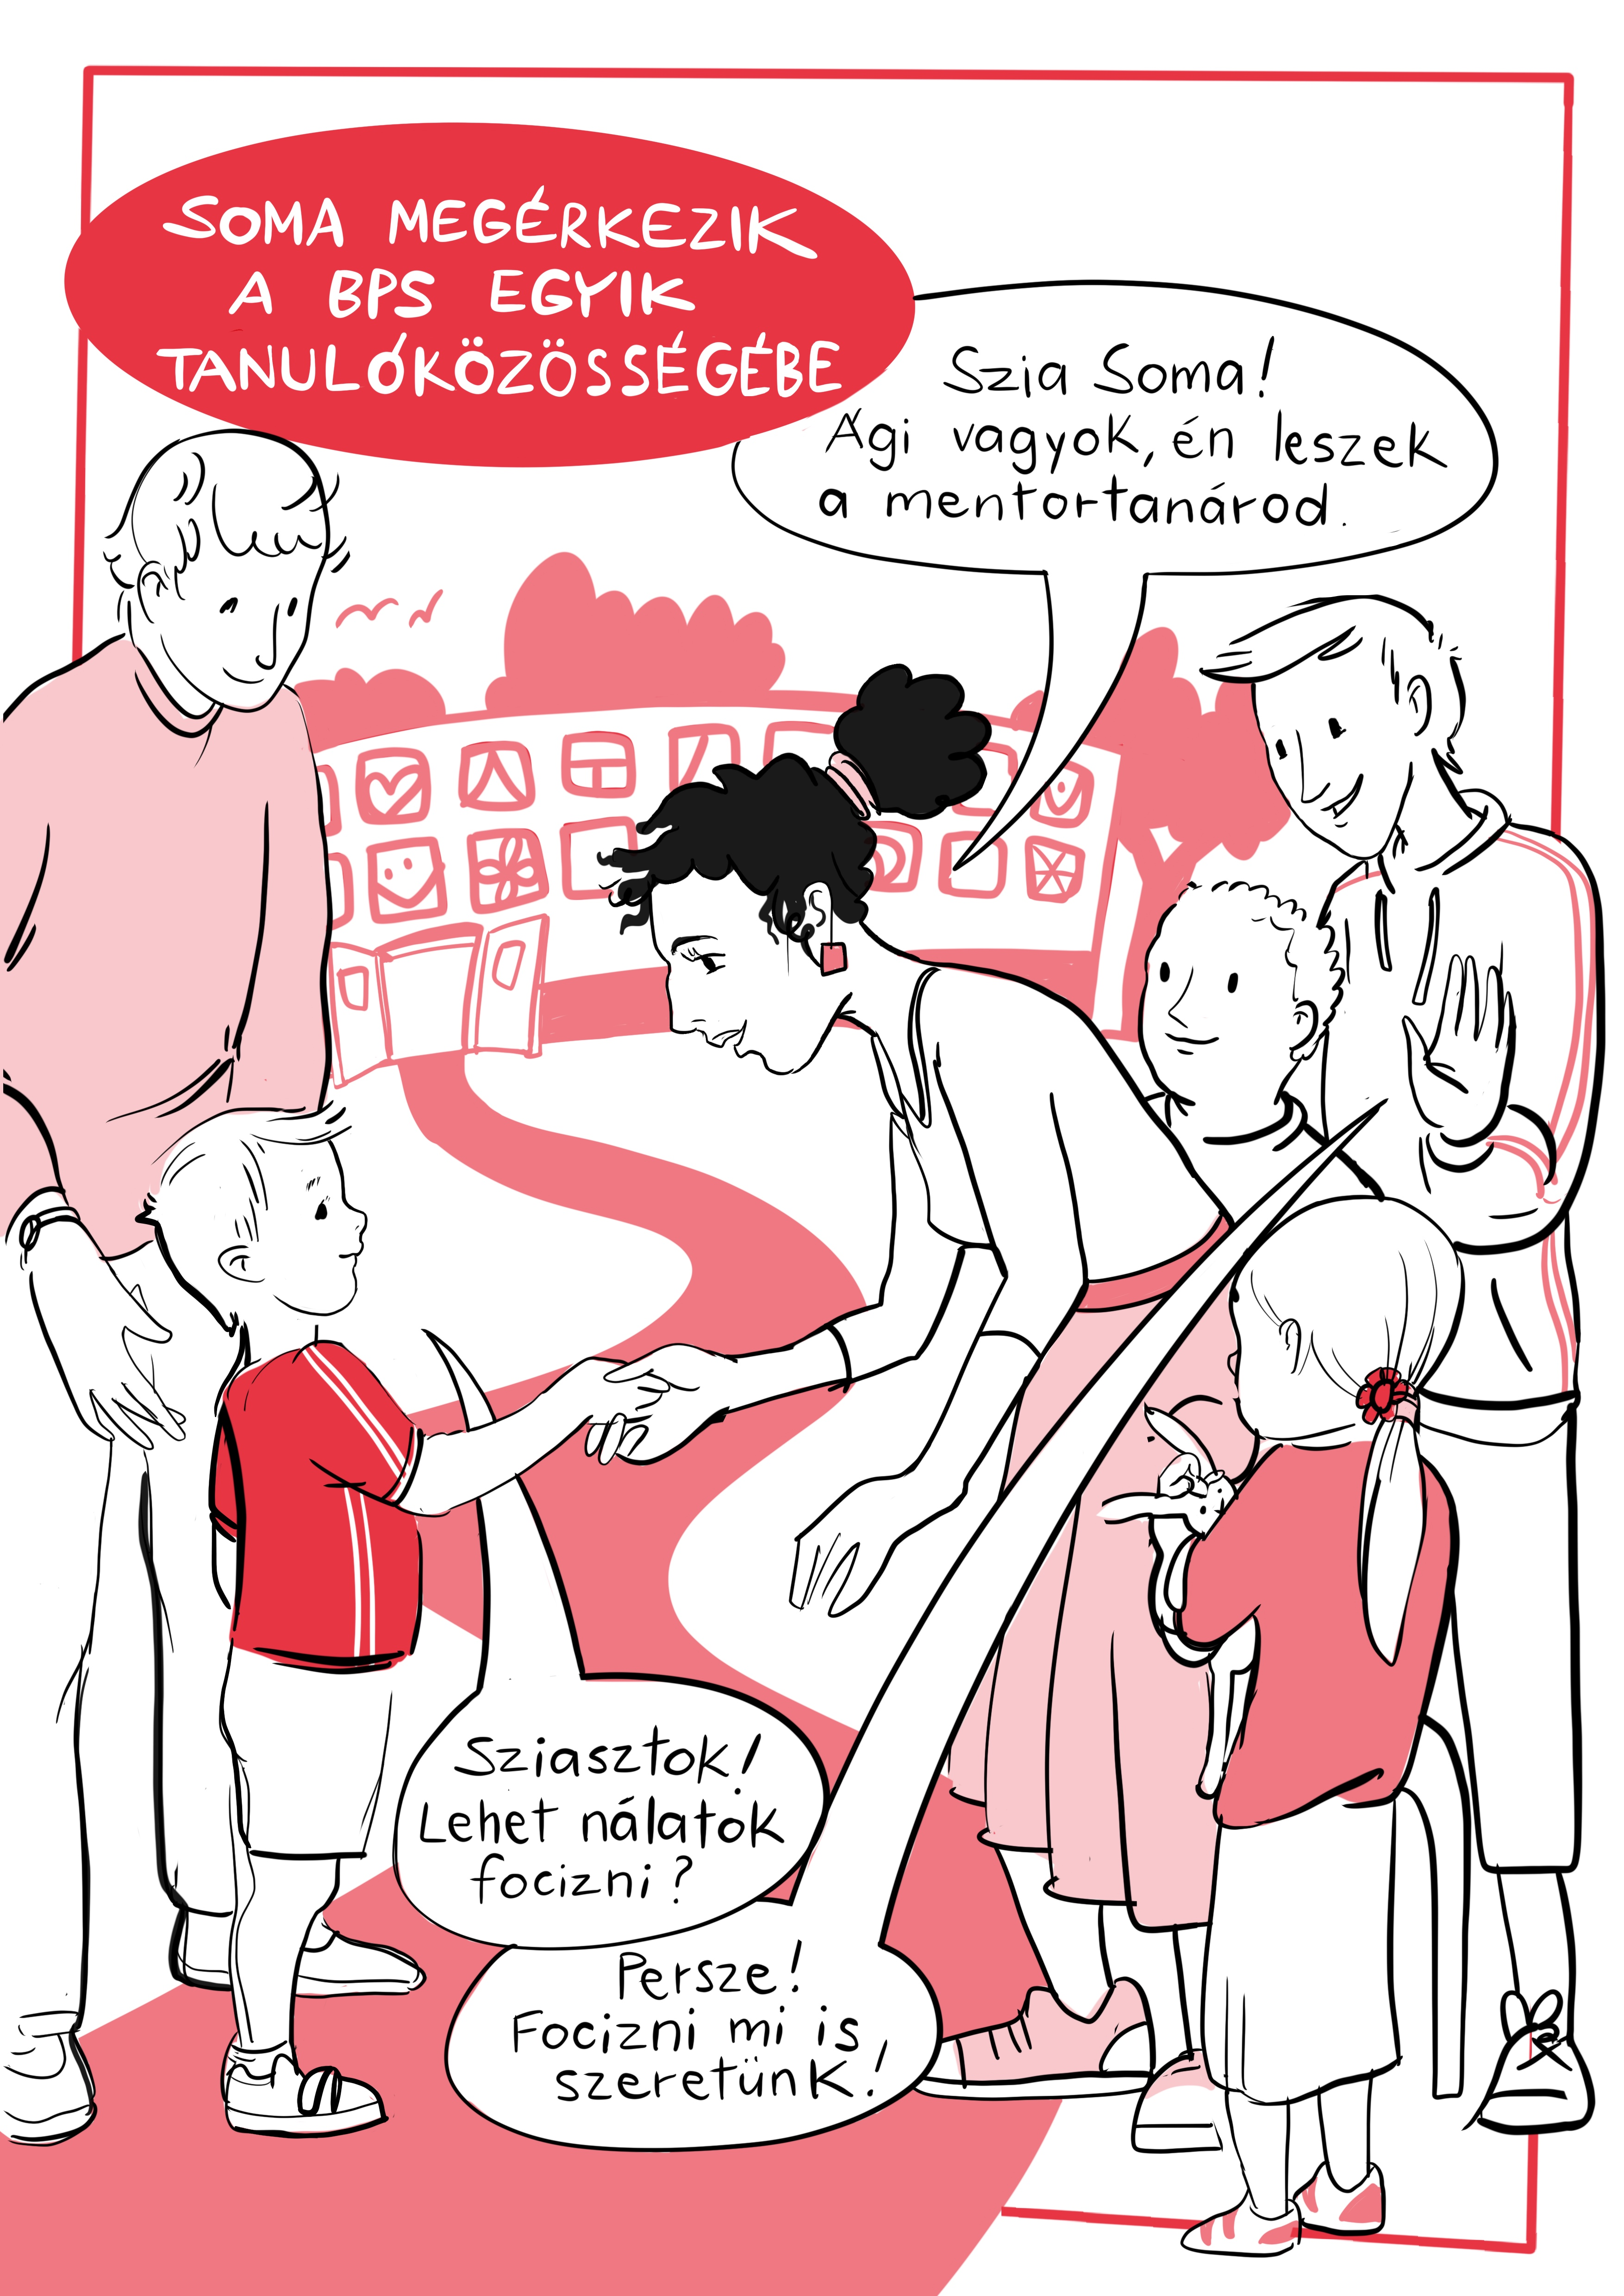
\includegraphics{pics/1a_mikroisk_soma.jpg}
\caption{A tanulóközösség egy gyerek elsődleges közössége.}
\end{figure}

\hypertarget{a-tanulokozossegeket-tanarok-vezetik}{%
\subsubsection{A tanulóközösségeket tanárok
vezetik}\label{a-tanulokozossegeket-tanarok-vezetik}}

A tanulóközösség fontos célja, hogy biztonságot, támogatást nyújtson, és
\emph{így} segítse a közösség tagjainak a minőségi tanulását. A
tanulóközösségeket tanárok irányítják, őket hívjuk tanulásszervezőknek.
Ők felelnek a tanulás tartalmáért, a foglalkozások meghirdetéséért és a
tanulási eredmények nyomon követéséért. Ők döntenek arról, hogy ki és
milyen feltétellel lehet tagja a közösségnek.

\hypertarget{a-tanulokozosseg-allando-a-gyerekek-es-a-tanarok-fluktuacioja-lehetseges}{%
\subsubsection{A tanulóközösség állandó, a gyerekek és a tanárok
fluktuációja
lehetséges}\label{a-tanulokozosseg-allando-a-gyerekek-es-a-tanarok-fluktuacioja-lehetseges}}

A tanulásszervező tanárok vagy gyerekek kilépése a tanulóközösség
fennállását nem érinti, helyettük a tanulóközösség új tanulásszervező
tanárt és gyereket vehet fel.

A tanulóközösség létrehozásakor arra kell törekedni, hogy olyan gyerekek
tanuljanak együtt, akik támogatni tudják egymást a tanulásban. A
gyerekek mindaddig a tanulóközösség tagjai, amíg ott jól tudnak tanulni,
és a közösség és a gyerek kapcsolata gyümölcsöző.

\begin{figure}
\centering
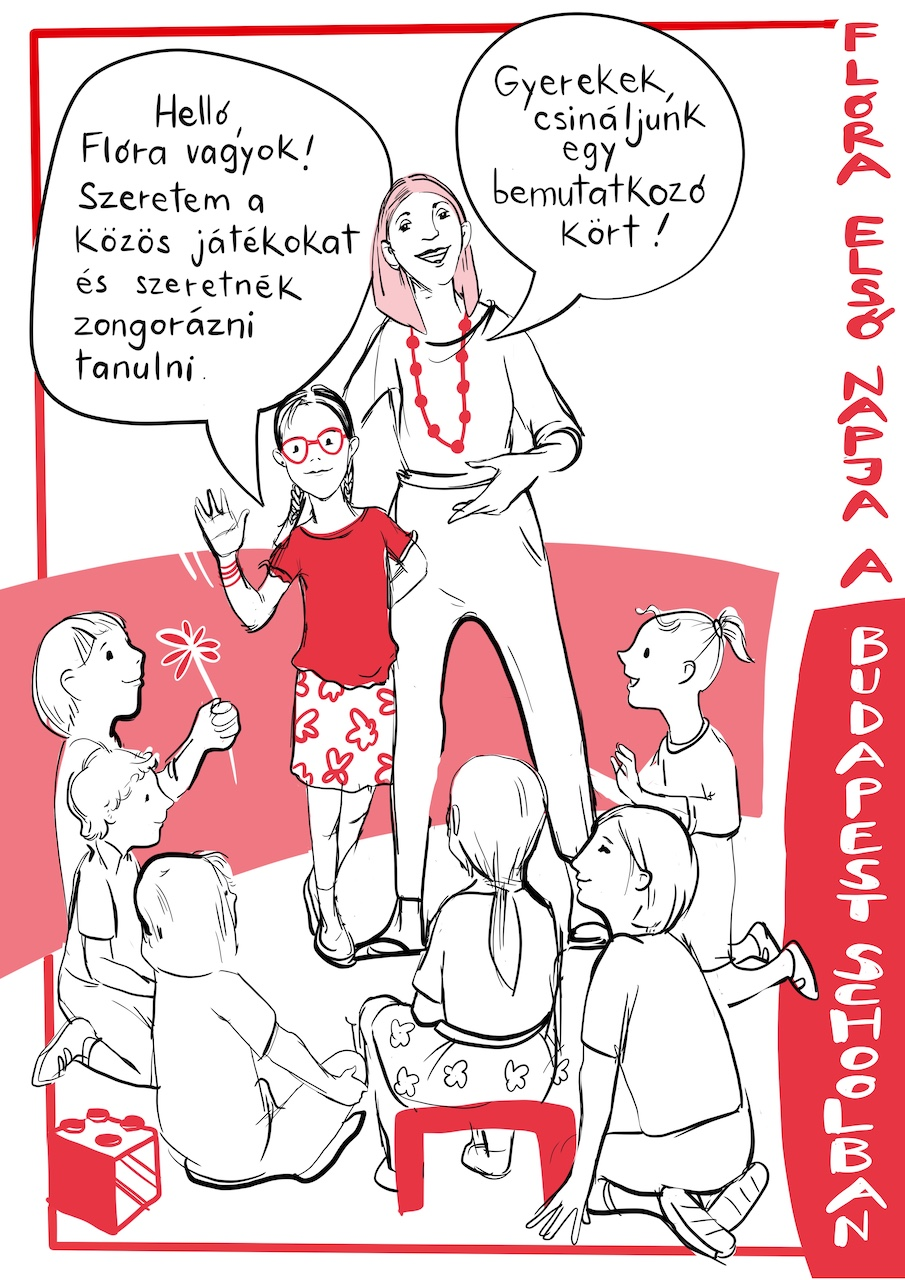
\includegraphics{pics/1b_mikroisk_flora.jpg}
\caption{A tanulóközösség egy családias közösség.}
\end{figure}

\hypertarget{a-tanulokozossegeknek-sajat-fokuszuk-helyszinuk-stilusuk-alakulhat-ki}{%
\subsubsection{A tanulóközösségeknek saját fókuszuk, helyszínük,
stílusuk alakulhat
ki}\label{a-tanulokozossegeknek-sajat-fokuszuk-helyszinuk-stilusuk-alakulhat-ki}}

A tanulóközösségek nemcsak abban térnek el egymástól, hogy kevert
korcsoportban, más korosztályú gyerekek, más érdeklődések mentén, és ily
módon más célokat követve tanulnak, hanem területileg, regionálisan is
eltérőek lehetnek.

A tanulóközösség-rendszerben lehetőség van arra, hogy adott tanulási
környezetben úgy váltakozhassanak a hangsúlyok a csoport és az egyén
érdeklődését követve, hogy közben fennmaradjon a tanulási egyensúly a
tantárgyak között. Ezért a tanulóközösségek órarendje, alkalmazott
pedagógiai módszerei, a tantárgyak összevonásának módja eltérő lehet.

Van olyan tanulóközösség, amely a fejlesztési célok eléréséhez és a
saját célok mentén már 6 éves gyerekek tanulásánál a robotika eszközeit
használja, másutt drámafoglalkozásokkal fejlesztik 12 éves gyerekek a
szövegértésüket és éntudatukat.

\hypertarget{a-tanulokozossegekben-a-gyerekek-nagymertekben-befolyasoljak-hogy-mit-es-hogyan-tanulnak-es-alkotnak}{%
\subsubsection{A tanulóközösségekben a gyerekek nagymértékben
befolyásol\\-
ják, hogy mit és hogyan tanulnak és
alkotnak}\label{a-tanulokozossegekben-a-gyerekek-nagymertekben-befolyasoljak-hogy-mit-es-hogyan-tanulnak-es-alkotnak}}

A tanulóközösségekben (a tanulásszervezők által meghatározott kereteken
belül) megfér egymással több, különböző saját céllal rendelkező gyerek
addig, amíg a tanulásszervezők minden gyerek számára biztosítani tudják
a tantárgyak által meghatározott tanulási eredmények elérését.

A tanulásszervezők feladata és felelőssége, hogy olyan közösségeket
építsenek, amelyek kellően diverzek, és mégis jól működnek. A
közösségnek a gyerekek igényeit és a NAT céljait egyaránt ki kell
elégítenie.

A tanulásszervezők választási lehetőségeket kínálnak (azaz modulokat
dolgoznak ki), amikből a gyerekek (a mentoruk és szüleik segítségével) a
saját céljaikat, érdeklődésüket leginkább támogató saját tanulási tervet
és utat alkotnak.

Eltérhet, hogy egy-egy gyerek mit tanul, ezért az is, hogy mikor és
hogyan sajátítja el a szükséges ismereteket: egy közösségben megfér a
központi felvételire fókuszáló 11 éves gyerek, és aki ekkor inkább a
Mi\-ne\-craft programozásában akar elmélyedni, ezért más képességek
fejlesztésével lassabban halad.

\hypertarget{csatlakozas-a-tanulokozossegekhez}{%
\subsubsection{Csatlakozás a
tanulóközösségekhez}\label{csatlakozas-a-tanulokozossegekhez}}

Arról, hogy egy gyerek csatlakozhat-e egy tanulóközösség közösségéhez, a
tanulásszervezők döntenek, figyelembe véve a gyerek életkorát, a
közösségben való eligazodását, érdeklődését, saját fejlődési igényét. A
kiválasztás fő elve, hogy a közösség fejlődjön minden gyerek
csatlakozásával.

\hypertarget{tanulokozossegek-osztalyai-es-csoportbontasai}{%
\subsection{Tanulóközösségek osztályai és
csoportbontásai}\label{tanulokozossegek-osztalyai-es-csoportbontasai}}

Egy tanulóközösségek minimális létszáma hat, maximális létszáma 60 fő, és
a tagok évfolyamszintje között maximum hat évfolyam lehet. Egy
tanulóközösségbe több osztály gyerekei tartozhatnak, de a
tanulóközösségek nem tekinthetőek összevont osztályoknak. Az egy
osztályba tartozó gyerekek tanulási célja nagyon hasonló, az évfolyamhoz
tartozó tanulási eredményeket el szeretnék érni.

A BPS mindennapjaiban a gyerekek a közösségeknél és az osztályoknál
nagyobb csoportban is tanulhatnak.

A tanulóközösségekben az idő legnagyobb részében a közösséget kisebb
csoportokra bontják a tanulásszervezők, hogy a tanulás hatékonyabb legyen.

\begin{itemize}
\tightlist
\item
  Egyes foglalkozások vagy modulok (tanulási-tanítási egységek) során
  egy-egy projektre szerveződnek, ilyenkor általában az eltérő képességű
  és életkorú gyerekek is kitűnően tudnak együtt dolgozni.
\item
  Más foglalkozások vagy modulok esetén a csoportokat a tanár
  képességszint alapján hozza létre. Ilyen csoportok lehetnek a
  másodfokú egyenletek megoldóképletét megismerő csoport, az írni
  tanulók csoportja, vagy egy angol nyelvű újság szerkesztésére és
  megírására alakult modul, ahol a nyelvismeretnek és a szövegalkotási
  képességnek már egy olyan szintjén kell állni, hogy a projektnek jól
  mérhető kimenete lehessen.
\item
  Vannak olyan foglalkozások és tanulási modulok, amikor kifejezetten az
  egy évfolyamra járó gyerekek tanulnak együtt, mert például a 9.
  évfolyamos matematikatanulási eredmények elérésén dolgoznak.
\end{itemize}

Több szintje van a csoportmunkának.

\begin{enumerate}
\def\labelenumi{\arabic{enumi}.}
\tightlist
\item
  A tanulóközösség közössége heti rendszerességgel tarthat
  iskolagyűlést, fórumot, plenárist, iskolakonferenciát. Ilyenkor a
  tanulóközösség közössége dolgozik együtt.
\item
  Egy tanulási modul csoportjának rendezőelve lehet:

  \begin{enumerate}
  \def\labelenumii{\alph{enumii}.}
  \tightlist
  \item
    egy képességszinten lévő gyerekek tanulnak együtt;
  \item
    a közös érdeklődés hozza össze a csoporttagokat;
  \item
    direkt a véletlenszerűségben van az érdekesség, mert keveredni
    akarnak;
  \item
    kölcsönös szimpátia és vonzalom a modultagok között: most azért
    vannak egy csoportban, mert egy csoportban akartak lenni.
  \end{enumerate}
\item
  Egy-egy foglalkozáson belül is sokszor csoportot alkotunk, az előző
  elvek alapján.
\end{enumerate}

Arra is lehetőség van, hogy egy csoport tagjai több tanulóközösség
tagjaiból álljanak össze, ha az támogatja a tanulást és az utazás
biztonságosan megoldható.

\hypertarget{kulonbozo-tanari-szerepek}{%
\section{Különböző tanári szerepek}\label{kulonbozo-tanari-szerepek}}

A Budapest Schoolban a gyerekek azokat a felnőtteket tekintik
tanáruknak, akik minőségi időt töltenek velük, és segítik, támogatják
vagy vezetik őket a tanulásukban. Több szerepre bontjuk a tanár
fogalmát: a gyerek legjobban egy felnőtthöz kapcsolódik, a
\emph{mentorához}, aki rá különösen figyel. A foglalkozásokon
megjelenhetnek további tanárok, a \emph{szaktanárok}, akik egy adott
foglalkozást, szakkört, órát, kurzust vezetnek. Szervezetileg minden
tanulóközösségnek van egy állandó \emph{tanárcsapata}, a
\emph{tanulásszervezők}, akik a mentorokból és a szaktanárokból állnak
össze. A tanulóközösség mindennapjait a tanulásszervezők határozzák meg.

A tanulásszervezők, mentorok legalább egy tanévre elköteleződnek,
szemben a szaktanárokkal, akik lehet, hogy csak egy pár hetes projekt
keretében vesznek részt a munkában. A tanulásszervezők általában
mentorok is, de nem minden esetben. Egy tanulásszervező lehet több
tanulóközösségben is ebben a szerepben, és így mentor is lehet több
tanulóközösségben.

\hypertarget{mentor}{%
\subsection{A mentor}\label{mentor}}

Minden gyereknek van egy \emph{mentora}, aki a saját céljainak
megfogalmazásában és a fejlődése követésében segíti. Minden mentorhoz
több gyerek tartozik, de nem több, mint 12. A mentor együtt dolgozik a
tanulóközösség többi tanulásszervezőjével, a szülőkkel és az általa
mentorált gyerekekkel. A mentor segít az általa mentorált gyereknek,
hogy a tantárgyi fejlesztési célok és a saját magának megfogalmazott
saját célok között megtalálja az egyensúlyt, és segít megalkotni a
gyerek \emph{saját tanulási tervét}.

A mentor a kapocs a Budapest School, a szülő és a gyerek között.

\begin{itemize}
\tightlist
\item
  Képviseli a Budapest Schoolt, a tanulóközösséget a szülő felé.
\item
    Ismeri a Budapest Schoolt, a lehetőségeket, a tanulásszervezés
    folyamatait.
\item
  Együtt tanul a többi Budapest School-mentorral, együtt dolgozik a
  tanártársaival.
\item
  Ismeri, segíti, képviseli a gyereket.
\item
  Az első trimeszter alatt a mentor megismeri mentoráltjának
  személyiségjegyeit, képességeit, érdeklődését, motivációit. Megismeri
  a mentorált családot.
\item
  Trimeszterenként a mentorált gyerekkel és szülőkkel egyetértésben
  kialakítja, majd folyamatosan monitorozza a mentorált gyerek
  haladását.
\item
  Tudja, hol és merre tart a mentoráltja, ismeri a képességeit,
  körülményeit, szándékait, vágyait.
\item
  Minimum kéthetente találkozik mentoráltjával. Követi, tudja, hogy a
  gyerek hogy érzi magát az iskolában, a családban, a mindennapokban.
\item
  Segít a saját célok elérésében, felügyeli a haladást.
\item
  Megerősíti a mentoráltjai pszichológiai biztonságérzetét.
\item
  Mentorként nyomon követi, monitorozza a mentoráltjai fejlődését, és
  szükség esetén továbblendíti, inspirálja őket. Visszajelzéseket ad a
  mentoráltjainak. A mentorált gyerekkel
  együtt rendszeresen reflektál 
  a tanulási céljaikra és haladásukra.
\item
  Segít abban, hogy az elért célok a portfólióba kerüljenek, biztosítja,
  hogy a mentorált gyerek portfóliója friss legyen.
\item
  Összeveti a portfólió tartalmát a tantárgyak fejlesztési céljaival, és
  jelzi, ha egy-egy tantárgyból hiány mutatkozik.
\item
  Segíti a mentorált választásait.
\item
  Együtt dolgozik, gondolkozik a szülőkkel, képviseli igényüket a
  közösség előtt.
\item
  Megállapodik a családdal a kapcsolattartás szabályaiban.
\item
  Bevezeti a családot a Budapest School rendszerébe.
\item
  Erős partneri kapcsolatot épít ki a szülőkkel.
\item
  Rendszeresen információt oszt meg.
\item
  Elérhető.
\item
  Asszertíven kommunikál.
\item
  Konkrét, specifikus, mérhető megállapodásokat köt.
\item
  Segít a gyerekekkel közös célokat állítani.
\item
  Amikor a gyereknek külső fejlesztésre, mentorra, tanárra, trénerre van
  szüksége, akkor a családot segíti a megfelelő segítő felkeresésében, a
  külsőssel kapcsolatot tart, és konzultál a mentoráltja haladásáról.
\item
  A szülő számára a mentor az elsődleges kapcsolattartó a különféle
  iskolai ügyekkel kapcsolatban.
\end{itemize}

A mentor egyszerre felelős a mentorált gyerek előrehaladásának
segítéséért, és közös felelőssége van a mentortársakkal, hogy az
iskolában a lehető legtöbbet tanuljanak a gyerekek. A mentor
folyamatosan figyelemmel követi az egyéni tanulási tervben
megfogalmazottakat, és ezzel kapcsolatos visszajelzést ad a mentoráltnak
és a szülőnek.

\hypertarget{szaktanarok}{%
\subsection{Szaktanárok}\label{szaktanarok}}

A szaktanárok egy-egy foglalkozás, vagy foglalkozássorozat, modul, azaz
tanulási egység megszervezéséért, lebonyolításáért felelnek. A
mentortanárok fő fókusza, hogy a gyerekek jól vannak-e. A szaktanárok fő
fókusza, hogy mit tanulnak a gyerekek. Ők segítik a gyerekeket egy
tanulási cél felé való haladásban akár egyetlen alkalommal, vagy éppen
egy egész trimeszteren át tartó tanulási, alkotási folyamatban.

Ők általában az adott tudományos, művészeti, nyelvi vagy bármilyen más
terület szakértői.

\begin{itemize}
\tightlist
\item
  Izgalmas, érdekes foglalkozásokat tartanak, amire felkészülnek, és amiben a
  gyerekeket flow-ban {\autocite{Csikszentmihalyi1991}} tudják tartani.
\item
  Amikor a gyerekek velük vannak, akkor folyamatosan dolgoznak,
  figyelnek, fókuszálnak, koncentrálnak, tanulnak.
\item
  Kedvesen és határozottan vezetik a csoportot, figyelnek arra, hogy
  mindenkit bevonjanak.
\item
  Változatos, gazdag módszertani eszköztárukból mindig a foglalkozáshoz
  megfelelő módszert tudják elővenni.
\item
  A foglalkozásaik fejlesztik a gyerekek kritikai gondolkozását,
  kreativitását, kommunikációját, úgy általában a 21. századi
  kompetenciákat {\autocite{Trilling2009}}.
\end{itemize}

\vspace*{.5ex}
\hypertarget{tanulasszervezo}{%
\subsection{Tanulásszervező}\label{tanulasszervezo}}

Egy tanulóközösséget vezető tanárok állandó tanári csapatát 1--12
tanulásszervező alkotja, akik egyedileg meghatározott szerepek mentén a
tanulóközösség mindennapjainak működtetéséért felelnek. A
tanulásszervezők tarthatnak foglalkozásokat, sőt kívánatos is, hogy
dolgozzanak a gyerekekkel, ne csak szervezzék az életüket. Ők rendelik
meg a külső szaktanároktól a munkát, ilyen értelemben a tanulási utak
projektmenedzserei.

\begin{itemize}
\tightlist
\item
  Kiszámítható, átlátható rendszert építenek, ahol a szülők és a gyerekek is
  biztonságban, informálva, bevonva érzik magukat.
\item
  A tanulási célokkal rezonáló foglalkozásokat, kurzusokat hirdetnek meg,
  szerveznek le.
\item
  A szülők és a gyerekek is érzik, értik, hogyan „történik'' a tanulás.
  Biztosítják számukra az átláthatóságot.
\item
  A szaktanároknak megadnak minden szükséges információt, kontextust, hogy
  hatékonyan tudják végezni a munkájukat.
\item
  Megadják a résztvevőknek az informált választás lehetőségét.
\end{itemize}

\hypertarget{a-kozos-szerepek}{%
\subsection{A közös szerepek}\label{a-kozos-szerepek}}

Minden BPS-es tanulásszervező, mentor és szaktanár egyszerre
\emph{csapattag}, \emph{BPS-tag}, \emph{EQ-nindzsa},
\emph{változásmenedzser (Change Agent)} és \emph{SNI-szakértő}.

\hypertarget{csapattag}{%
\paragraph{Csapattag}\label{csapattag}}

\begin{itemize}
\tightlist
\item
  Rendszeresen jelen van a tanári csapat megbeszélésein.
\item
  El lehet érni telefonon vagy online, a csapattal megállapodott
  kereteken belül.
\item
  Feladatokat vállal magára, és azokat megbízhatóan, határidőre
  végrehajtja.
\item
  Kooperatív és támogató a közös munkák, ötletelések, megbeszélések
  alatt, képviseli a saját nézőpontját, gondolatait, érzéseit, miközben
  a csapat és a többiek igényeire is figyel.
\item
  Kifejezi támogatását, ellenérveit és javaslatait a jobb megoldás
  érdekében.
\item
  A visszajelzést keresi, a kritikát jól fogadja, és megfontolja,
  átgondolja a lehetséges változtatásokat.
\item
  A kollégák fejlődését segíti rendszeres visszajelzésekkel.
\end{itemize}

\hypertarget{bps-tag}{%
\paragraph{BPS-tag}\label{bps-tag}}

\begin{itemize}
\tightlist
\item
  Rendszeresen jelen van a közös tanári eseményeken.
\item
  Részt vesz a tanulóközösségének és a Budapest Schoolnak a
  fejlesztésében.
\item
  Proaktívan alakít ki rendszereket, folyamatokat, és a legjobb
  gyakorlatokat megosztja BPS-szinten.
\item
  Közös témákban aktív, hozzászól, alakítja a véleményével és tudásával
  a BPS rendszerét.
\end{itemize}

\hypertarget{az-erzelmi-intelligencia-eq-nindzsa}{%
\paragraph{Az érzelmi intelligencia (EQ-nindzsa)}\label{az-erzelmi-intelligencia-eq-nindzsa}}

\begin{itemize}
\tightlist
\item
  A gyerekek pszichológiai biztonságérzetét megerősíti.
\item
  Olyan visszajelzéseket ad, amelyek az erőfeszítésekre, a befektetett
  energiára, munkára és a jövőbeni fejlődésre fókuszálnak (growth
  mindset), pozitív megerősítést alkalmaz, épít a gyerek erősségeire, és
  egyértelműen megfogalmazza, mit tehetne másként.
\item
  Odaforduló, barátságos, nyitott.
\item
  Munkája során gondoskodik a gyermek személyiségének, énképének,
  énhatékonyságának fejlődéséről.
\item
  Figyelembe veszi a gyerekek egyéni képességeit, adottságait,
  fejlődésének ütemét, szociokulturális helyzetét.
\item
  Előmozdítja a gyerek erkölcsi fejlődését.
\item
  Segít a gyerekeknek jobban működni a csoportban.
\end{itemize}

\hypertarget{sni-szakerto}{%
\paragraph{SNI-szakértő}\label{sni-szakerto}}

\begin{itemize}
\tightlist
\item
  Jól tudja kezelni az egyéni, különleges bánásmódot, speciális nevelést
  igénylő gyerekeket a csoportban.
\item
  A különleges bánásmódot igénylő gyermekek családjával, a nevelést,
  oktatást segítő más szakemberekkel együttműködik, hogy a\break
  gyerek
  támogatása minden esetben megtörténjen.
\item
  Akinek külső segítségre van szüksége, azoknak a szüleivel ezt
  proaktívan egyezteti, és menedzseli a folyamatot.
\end{itemize}

\hypertarget{change-agent}{%
\paragraph{Change agent}\label{change-agent}}

\begin{itemize}
\tightlist
\item
  A nehézségeken könnyen továbblendül. Megtalálja a kiégés ellenszerét,
  tudatosan keresi a feltöltődés alkalmait és lehetőségeit.
\item
  Nemcsak a problémákra, hanem a megoldásokra keresésére is odafigyel.
  Keresi, hogy mire lehet hatása, mit tud előremozdítani, és meg is
  teszi a szükséges lépéseket.
\item
  Felismeri, elismeri és megünnepli az előrelépéseket, a közös
  sikereket.
\end{itemize}

\hypertarget{tanulasi-tanitasi-egysegek-a-modulok}{%
\section{Tanulási-tanítási egységek, a
modulok}\label{tanulasi-tanitasi-egysegek-a-modulok}}

A \emph{tanulási-tanítási egységek}, a Budapest School Modell
szóhasználatában a \emph{modulok} a tanulásszervezés
\emph{alapegységei}: olyan foglalkozások megtervezett sorozata, amelyek
során egy meghatározott időn belül a gyerekek valamely képességüket
fejlesztik, valamilyen ismeretet elsajátítanak, vagy valamilyen
produktumot létrehoznak. A tanítási egységek célja sokféle lehet, de
kötelező elvárás, hogy a résztvevők a portfóliójukba való bejegyzésre érdemes
eredményt hozzanak létre, és hogy legyen egyértelmű céljuk.

A modulok tehát önálló céllal, fókusszal, kerettel bíró
foglalkozásegységek. Akár szakköröknek, workshopoknak,
mikrotantárgyaknak, projekteknek vagy foglalkozásoknak is hívhatnánk őket. A BPS modell a
legsemlegesebb szót akarja az használni, hogy a tanárok és a gyerekek
tudják feltölteni tartalommal a modulokat.

\hypertarget{a-modulok-a-tanmenet-egysegei}{%
\subsubsection{A modulok a tanmenet
egységei}\label{a-modulok-a-tanmenet-egysegei}}

A modulok fogalmat a NAT és az Nkt.\ is ismeri. Ezekben a jogszabályokban
tantárgyi témaköri egységet jelentenek, bár maga a NAT nem definiálja a
fogalmat. A BPS modellben a modul csak annyit jelent: összefüggő
foglalkozások egysége, azaz a tanulási-tanítási egységet és a modul
szavakat szinonimaként kezeli. Ha a diszciplináris tanítás egysége
diszciplináris modul, a multidiszciplináris tanítás egysége
multidiszciplináris modul.

A BPS modellben kétféle tervezéstípust ötvözünk:

\begin{enumerate}
\def\labelenumi{\arabic{enumi}.}
\tightlist
\item
  a hosszú távú célokból kiinduló, majd azt a szakaszosan a mindennapokra
  lebontó felülről lefelé tervezést ötvözzük
\item
  az elsődlegesen a gyerekek élményére fókuszáló és abból építkező
  lentről felfelé való tervezési megközelítéssel.
\end{enumerate}

Az előbbi megközelítésben a tantervi célokból alakulnak a tantárgyak,
azokat tematikára, tematikus egységekre bontjuk. Ebből alakulnak ki
tanítási egységek, majd foglakozásokra bontva alakul ki a gyerekek
élményének megtervezése. Ezt hívhatjuk felülről-lefele (angolul
top-down) tervezésnek. A lentről-felfelé (bottom-up) tervezéssel pedig
a kívánt gyerek-élménytől indulunk ki, és a tanulási-tanítási
egységekből építjük újra fel a tantárgyak tartalmát, illetve az elvárt
tanulási eredményeket.

Például \emph{A koronavírus terjedése} című foglalkozás elvezethet oda,
hogy a gyerek \emph{mértani sorozatokra vonatkozó ismereteit használja
gazdasági, pénzügyi, természettudományi és társadalomtudományi problémák
megoldásában.} Fentről-lefelé tervezés ehhez a foglalkozáshoz úgy
jutott, hogy az 9--12. évfolyam Matematika tantárgy céljaiból levezette,
hogy foglalkozni kell a mértani sorozatokkal társadalmi változások
elemzéséhez. A tanár úgy gondolta, hogy nem a kamatos kamattal
foglalkozik, hanem a gyerekek számára éppen érdekesebb koronavírussal,
azaz cél eléréséhez a gyerekek érdeklődése mentén talált utat.

A lentről felfelé tervezés pedig a gyerekek érdeklődéséből indul ki, ami
jelen esetben a koronavírus. És esetleg később veszi észre a tanár és a
gyerek, hogy már az 9--12. Matematika elvárásainak egy részét is
teljesítették. Hisz ez előre nem volt tervezve, mert a cél nem a
tantárgyi követelmények teljesítése volt, hanem a téma feldolgozása.

A két tervezési módot ötvözi a BPS modell. Az agilis tervezés
eredményeképp feltehetőleg az alulról felfelé tervezés indul meg: itt és
most mire van igényük a gyerekeknek. Idővel, például az év vége fele,
vagy az érettségi vizsgához közeledve egyre erősebb lesz a fentről
lefelé tervezés, és ez így van helyén. Ott és akkor az a kérdés merül
fel, hogy mire van még szükség, hogy azokat a célokat is elérjük. De az
is előfordulhat, hogy egy közösség inkább fentről lefelé tervezne:
biztos, ami biztos, érjük el a tantárgyi célokat, és az úton legyünk
kreatívak, vagy épp akkor, amikor már a szükséges eredményeket biztos
elértük.

\emph{A fentről lefelé vagy lentről felfelé tervezés során létrejövő
tanulási-ta\-ní\-tá\-si egységeket, a tanmeneteket építő egységeket hívja a
BPS modell moduloknak.}

\hypertarget{foglalkozasok-modulok---szohasznalat-definiciok}{%
\subsection{Foglalkozások, modulok - szóhasználat,
definíciók}\label{foglalkozasok-modulok---szohasznalat-definiciok}}

Bár a BPS modell a modulok szintjén írja le a tanulás-tanítás élményét,
a tanulási élmény leginkább meghatározó elemei mégis a
\emph{foglalkozások}. Az a dedikált idő, amit a (szak)tanár és a gyerek
azért alakítanak ki, hogy a gyerek tanuljon. A modul nem más, mint
egybefüggő foglalkozások sorozata. Ezért a BPS modellben, ahol a \emph{modul}
szót használjuk, ott a \emph{foglalkozás} szót is használhatnák.

A BPS modell nem a tanóra szót használja, hogy kihangsúlyozza: egy
foglalkozás célja nem csak egy adott tantárgy következő témakörének
feldolgozása lehet. Foglalkozás többek közt lehet

\begin{enumerate}
\def\labelenumi{\arabic{enumi}.}
\tightlist
\item
  tantárgycsoportok összevont foglalkozása;
\item
  témanapok, témahetek eseményei;
\item
  projektekben való dolgozás;
\item
  önálló tanulás, gyakorlás;
\item
  közös önálló tanulás, tanulószobai tevékenység;
\item
  vagy épp egy tantárgy témakörének feldolgozása.
\end{enumerate}

A foglalkozások tanügyigazgatási értelemben megegyeznek a tanórákkal. A
foglalkozások hossza különböző lehet a törvények által megadott keretek
között. A foglalkozások tanórának számolhatók el, ha tantárgyi tartalom
elsajátítása a céljuk. Ha több tantárgy tartalmát érinti a foglalkozás,
akkor több tantárgy tanórájának számolandó el.

\hypertarget{modulok---a-tantargyak-kozott-szabadon-mozoghatunk}{%
\subsubsection{Modulok --- a tantárgyak között szabadon
mozoghatunk}\label{modulok---a-tantargyak-kozott-szabadon-mozoghatunk}}

A Budapest School Modell hangsúlyozza a tanulási-tanítási egység, a
modulok szerepét, ezért nevezi a tanmenetet \emph{moduláris
tanmenetnek}. Ugyanazt az eredményt éri el egy tanár, aki egy tantárgy
tanóráinak egyes egységeire külön foglalkozásokat tervez (és akár
külső előadókat, tanárokat is meghív besegíteni), mint az a tanár, aki
tanulási-tanítási egységeket, modulokat tervez, és ezekből építi fel a
tanévet.

Egy tanulási-tanítási egység több tantárgy tananyagtartalmát is
lefedheti.

A mindennapi tanulás a tanulás-tanítási egységek, a modulok elvégzésével
történik, ezzel biztosítva, hogy rugalmas keretek között, pontosan
megfogalmazott célok mentén, a gyerekek számára érthető, átlátható és
sajátnak megélt tartalommal történjen.

A tanulási-tanítási egységeket, vagyis a tanulás tartalmának és
formájának alapegységét a tanulásszervezők három kötelező összetevőből
állítják össze:

\begin{enumerate}
\def\labelenumi{\arabic{enumi}.}
\item
  a NAT tantárgyainak tartalmából;
\item
  a gyerekek, tanárok érdeklődéséből, aktuális tudásából;
\item
  és a környezetük és a világ aktuális kihívásaiból.
\end{enumerate}

A három komponensből a legelső a legstatikusabb, hiszen a NAT
meghatározza a tantárgyakat és azok tartalmát, valamint azt, hogy milyen
lehetséges eredmények elérését várjuk az ezekben való fejlődéstől. Az
egyes tanítási egységekban ezek személyre, illetve a csoport igényeire
szabhatóak, hiszen az elérhető eredményeket különféle gyakorlati és
elméleti tanulási módszerekkel el lehet érni.

A gyerekek és tanárok érdeklődése --- ami a sajátként megélt cél és a
minél nagyobb fokú bevonódás alapfeltétele --- alakítja ki a tanítási
egységek témáját, a projekteket, és a gyerekek egyéni tanulási idejét is
meghatározhatja.

Mindemellett az iskola szándéka, hogy a tanárok, gyerekek reagáljanak a
környezetükre, a világ aktuális kihívásaira, kérdéseire. A NAT
meghatározza például, hogy a gyerek \emph{„Problémákat old meg
táblázatkezelő\break
program segítségével.''}. Az azonban, hogy a gyerekek
milyen táblázatokat szerkesztenek szívesen, csak a tanítási egységek
összeállításakor és a tanítási egységek elvégzése során derül ki. Nagyon
hasonló táblázatkezelési képességeket lehet fejleszteni, ha valaki az
önvezető autóktól várt csökkenő számú balesetekről , vagy ha az egy főre
jutó károsanyag-kibocsátás és a GDP-növekedés alakulásának arányáról
készít táblázatot.

A tanulási-tanítási egységekben épülő moduláris tanmenet fő célja, hogy
egyszerre képes legyen alkalmazkodni a menet közben felmerülő tanulási
igényekhez, adjon átlátható struktúrát a tanulásnak, és hogy a
tanulóközösség minél rugalmasabban tudja támogatni a tanulást úgy, hogy
a saját, a közösségi és a társadalmi célok harmóniába kerülhessenek.

Ez is mutatja, hogy bár közösek a kereteink, végtelen az elképzelhető
tanítási egységek (a tanulási utak építőkövei, és így a különböző
tanulási utak) száma. Ezért tartja fontosabbnak a Budapest School Modell
annak meghatározását, hogy hogyan kell a tanítási egységeket, a
modulokat létrehozni, mint azt, hogy a tanítási egységeket, a modulokat
tételesen felsorolja.

\hypertarget{modulok-sokfelek-lehetnek}{%
\subsubsection{A modulok sokfélék
lehetnek}\label{modulok-sokfelek-lehetnek}}

Egy-egy tanítási-tanulási egység, azaz egy modul során a gyerekek
képesek

\begin{itemize}
\tightlist
\item
  produktum létrehozására szerveződő projektben részt venni;
\item
  felfedezni, feltalálni, kutatni, vizsgálni, azaz kérdésekre választ
  keresni;
\item
  egy jelenséget több nézőpontból megismerni;
\item
  valamely képességüket, készségüket fejleszteni;
\item
  adott vizsgára gyakorló feladatokkal felkészülni;
\item
  közösségi programokban részt venni;
\item
  az önismeretükkel, a tudatosságukkal, a testi-lelki jóllétükkel
  foglalkozni.
\end{itemize}

\hypertarget{tantargyi-es-multidiszciplinaris-modulok}{%
\subsubsection{Tantárgyi és multidiszciplináris
modulok}\label{tantargyi-es-multidiszciplinaris-modulok}}

Egyes modulok, a \emph{tantárgyi modulok} célja egy tantárgy
ismereteinek elsajátítása, vagy egy-egy tantárgyi vizsgára, pl.
érettségi vizsgára való felkészülés. A tantárgyi modulokat tantárgyi
szaktanárok tartják.

A \emph{multidiszciplináris modulok} esetén több tantárgy ismereteinek
integrálását igénylő (multidiszciplináris) téma kerül a középpontba. A
multidiszciplináris modulok tervezéséhez erős szempontot adnak a
% \href{/tanulas-megkozelitese/kiemelt-fejlesztesi-teruletek.md}
{\emph{kiemelt
fejlesztési területek}}.

\hypertarget{orabontasok-csoportbontasok-osztalyok}{%
\subsection{Órabontások, csoportbontások,
osztályok}\label{orabontasok-csoportbontasok-osztalyok}}

Egy foglalkozás megszervezhető különböző évfolyamok, különböző osztályok
tanulóiból álló csoportok részére is, ahogy azt a 20/2020. EMMI rendelet
13 § (1) is kimondja. Ebben az esetben a foglalkozások differenciált és
kooperatív tanulásszervezést igényelnek.

Ebből következik, hogy egy modul, azaz a foglalkozások sorozata is
megszervezhető különböző évfolyamok, különböző osztályok tanulóiból álló
csoportok részére is.

\hypertarget{a-modulok-meghirdetese}{%
\subsection{A modulok meghirdetése}\label{a-modulok-meghirdetese}}

A tanulási-tanítási egységek kiválasztása, felkínálása a
tanulásszervezők feladata, hiszen ők figyelnek és reagálnak a gyerekek,
szülők céljaira és igényeire. A meghirdetett tanítási egységekből áll
össze a tanulás trimeszterenkénti tanulási rendje.

A tanulásszervezők az egyes tanulási-tanítási egységek tematikáját,\break
hosszát és feladatát a gyerekek tanulási céljainak megismerését követően
és a NAT-ban meghatározott tantárgyi tanulási eredményeket figyelembe véve
határozzák meg.

A tanulási-tanítási egységekbe, modulokba való csatlakozásról a mentor,
a szülő és a gyerek közösen dönt, mindig szem előtt tartva, hogy
folyamatos előrelépés legyen a már elért egyéni és tantárgyi
eredményekben is. Egy modul megkezdésének lehet feltétele egy korábbi
modul elvégzése, a gyerek képességszintje, a jelentkezők száma, és lehet
egyedüli feltétele a gyerekek érdeklődése.

Egy szaktanár különféle tematikájú tanítási egységeket tarthat attól
függően, hogy a saját célok, a tantárgyi eredmények mit kívánnak, és
hogy a
tanulásszervezők, valamint a szaktanárok kapacitása mit enged meg.

Amikor egy gyerek moduljai befejeződnek, és újat vesz fel, a
tanulásszervező feladata a gyereket segíteni abban, hogy az érdeklődési
körének, tanulási céljainak, és a soron következő, még el nem ért
tantárgyi eredményekben való fejlődéshez megfelelő tanítási egységek
közül választhasson.

A tanulásszervezők feladata a tantárgyi eredményelvárások nyomon
követése is. A tanítási egységek kidolgozásához és azok megtartásához
külsős szakembereket is meghívhatnak, azonban ilyenkor is a
tanulásszervezők felelnek azért, hogy a tanítási egységekkal elérni
kívánt tanulási célok teljesüljenek.

\hypertarget{a-modulok-egysegek-formatuma}{%
\subsection{A modulok, egységek
formátuma}\label{a-modulok-egysegek-formatuma}}

A moduláris rendszer elég nagy szabadságot ad a tanároknak abban, hogy
hogyan szervezik a mindennapokat. Ezért is fontos, hogy már a modul
meghirdetése előtt néhány szempont szerint kialakítsák a tanítási
egységek kereteit.

\hypertarget{celok}{%
\paragraph{Célok}\label{celok}}

Minden tanulási-tanítási egységnek, modulnak előre meg kell határozni a
célját. A tanulási szerződések célkitűzéseihez hasonlóan itt is minél
specifikusabban és mérhetőbben kell megfogalmazni a célokat. Javasolt az
OKR {\autocite{Doerr2018}} vagy a SMART {\autocite{Doran1981}} technika
alkalmazása, hogy minél specifikusabb, teljesíthetőbb, tervezhetőbb és
köny-\break
nyen mérhető célokat tűzzenek ki.

\hypertarget{ertekeles}{%
\paragraph{Értékelés}\label{ertekeles}}

A tanulási-tanítási egység végén minden résztvevő személyes, több
szempont alapján készült értékelést, visszajelzést kap a
tanulási-ta\-ní\-tá\-si egységgel kapcsolatos tevékenységére és elért
eredményeire. A visszajelzés struktúráját előre meg kell határozni, és
még a modul kezdete előtt meg kell osztani a résztvevőkkel.

Természetesen a visszajelzés szempontjai változhatnak a
tanulási-ta\-ní\-tá\-si egység során, ha változik a tanulási-tanítási egység
tartalma, szempontjai. Ebben az esetben ezt mindenki számára nyilvánvalóvá
kell tenni.

\hypertarget{idotartam}{%
\paragraph{Időtartam}\label{idotartam}}

Egy-egy tanulási-tanítási egység hossza és a tanulási-tanítási egységhez
kapcsolódó foglalkozások száma és gyakorisága változó: egy alkalomtól
legfeljebb egy teljes trimeszteren keresztül tarthat. A
tanulási-tanítási egység végén a tanulásszervező és a gyerek(ek) a
modult lezárják, értékelik és az elért eredményeket rögzítik a
(tanulási) portfólióban. Egy tanulási-tanítási egység folytatásaként a
következő trimeszterben új tanulási-tanítási egységet alakítanak ki a
tanárok.

\hypertarget{modszertan-formatum}{%
\paragraph{Módszertan, formátum}\label{modszertan-formatum}}

A tanulási-tanítási egységek nemcsak témájukban, céljaikban,
időtartamukban, hanem módszertanukban, folyamataikban is különbözhetnek:
bizonyos tanulási-tanítási egységekben a felfedeztető (inquiry based)
módszer, másokban az ismétlő (repetitív) gyakorlás a célravezető. Így
mindig a tanulási-tanítási egység céljához, a tanárok és a gyerekek
képességeihez és igényeihez választható a legjobb módszer.
Tanulási-tanítási egységenként változhat, hogy a folyamatot a gyerekek
vagy a tanárok befolyásolják-e, és milyen mértékben. Két példa az
eltérésre:

\begin{enumerate}
\def\labelenumi{\arabic{enumi}.}
\item
  Egy digitális kézműves tanulási-tanítási egység célja, hogy építsünk
  valamit, ami programozható. Annak kitalálása, hogy mit és hogyan
  építünk, a gyerekek feladata. Itt a tanár csak támogatja a tanulás
  folyamatát, azaz \emph{facilitál}.
\item
  Egy „\emph{A vizuális kommunikáció fejlődése a XX. század második
  felében}'' tanulási-tanítási egység esetén a tanár előre felépíti a
  tanmenetet, például hogy mely alkotók munkásságát, alkotásait fogja
  bemutatni, és ezeket a gyerekekkel sorban végigveszi. Ilyenkor is
  bővülhet azonban a tematika a gyerekek érdeklődése, felvetései mentén.
\end{enumerate}

\hypertarget{a-tanulasi-tanitasi-egysegek-helyszine}{%
\subsection{A tanulási-tanítási egységek
helyszíne}\label{a-tanulasi-tanitasi-egysegek-helyszine}}

A tanulás az egyes tanulóközösségek helyszínén, egy másik Budapest\break
School-épületben, a tanár által kiválasztott külső helyszínen, vagy akár
online, virtuális térben történik. A tanulásra úgy tekintünk, mint az
élethez szorosan kapcsolódó holisztikus fejlődési igényre, melynek
jegyében az elsődleges szocializációs térről és formáról, a szülői,
családi környezetről sem akarjuk a tanulást leválasztani. Az élethosszig
tartó tanulás jegyében a tanulás tere az iskolai időszak után és az
iskola terein kívül is folytatódik.

A gyerekek több ok miatt is tanulnak az iskolán kívül:

\begin{enumerate}
\def\labelenumi{\arabic{enumi}.}
\item
  tanulási-tanítási egységek foglalkozásai szervezhetők külső
  helyszínekre, úgymint múzeumokba, erdei iskolákba, parkokba,
  vállalatokhoz, vagy tölthetik az idejüket „kint a társadalomban''.
\item
  Amennyiben ez saját céljuk elérését nem veszélyezteti, és a folyamatos
  fejlődés biztosított, a mentoruk tudomásával a gyerekek az
  önirányított tanulás elvére figyelemmel a telephelyen kívüli egyéb
  helyszínen is elvégezhetnek egy-egy tanulási-tanítási egységet.
\end{enumerate}

A tanulási-tanítási egység lezárásaként a gyerekek és tanárok
visszajelzést adnak egymásnak, aminek része, hogy megosztják saját
élményeiket, reflektálnak a közös időre, összegyűjtik és értékelik az
elért eredményt, és kitérnek az esetleges fejlődési lehetőségekre.

\hypertarget{kulsos-tanarok-aranya}{%
\subsection{Külsős tanárok aránya}\label{kulsos-tanarok-aranya}}

A pedagógiai program egy fontos megkötést ad a tanulási-tanítási
egységek megtartására: a tanulóközösség tanulásszervezőinek kell
vezetniük a gyerekek moduljainak nagy részét.  Másképp fogalmazva:
korlátozva van a külsős, nem tanulásszervezők által tartott modulok
óraszáma, ahogy ezt a lenti táblázat mutatja. Ennek a megkötésnek az az
oka, hogy

\begin{itemize}
\item
  Kisebb korban szeretnénk, ha kevesebb, állandóan jelenlévő felnőtt
  vezetné a gyerekek tanulását (a kéttanítós rendszer mintájára).
\item
  Biztosított legyen, hogy a gyerekek a tanulóközösség
  tanulásszervezőiel elegendő időt töltsenek.
\item
  Érettségihez közeledve legyen lehetőség minél több külsős, akár\break
  speciális szaktudással bíró embertől tanulni.
\end{itemize}

%% \renewcommand{\arraystretch}{1.5}
%% \begin{longtable}[]{l*{5}{|l}}
%% \bfseries Évfolyamszint &\bfseries 1--2 &\bfseries 3--4 &\bfseries 5--8 &\bfseries 9--11 &\bfseries 11--12\tabularnewline
%% \hline
%% „Belsős'' modulok min. aránya& 70\% & 60\% & 55\% & 50\% &
%% 40\%\tabularnewline
%% \end{longtable}

\begin{longtable}[]{@{}llllll@{}}
\toprule
Évfolyamszint & 1--2 & 3--4 & 5--8 & 9--11 & 11--12\tabularnewline
\midrule
\endhead
„Belsős'' modulok min. aránya & 70\% & 60\% & 55\% & 50\% &
40\%\tabularnewline
\bottomrule
\end{longtable}

\hypertarget{modulok-nyomonkovetese}{%
\subsection{Modulok nyomonkövetése}\label{modulok-nyomonkovetese}}

Minden trimeszter megkezdésekor a tanulásszervező tanárok meghirdetik a
kötelező, a kötelezően választható és a választható modulokat, azaz
rögzítik, hogy

\begin{itemize}
\item
  ki a modul vezetője, és melyik pedagógus munkakörben alkalmazott
  tanulásszervező felelős (elszámoltatható a
  %\href{https://www.pmsz.hu/hirek-aktualitasok/havi-mustra/havi-mustra-a-felelosseg-hozzarendelesi-matrixrol}
  {\emph{RACI}}
  menedzsment
  rendszer értelmezésében) a modulért;
\item
  mi a modul célja, keretei és várható eredményei;
\item
  hol, mikor és milyen rendszerességű foglalkozások lesznek;
\item
  és mi a részvétel feltétele (előzetes tudás, kor, maximum létszám),
  azon belül, hogy teljes folyamatra kell-e
  elköteleződni, vagy esetileg is lehet a modult látogatni.
\end{itemize}

Ezután eldől, hogy ki mikor melyik modulon vesz részt. Ennek rendszerét
a tanárok alakítják ki: beoszthatják a gyerekeket, ahogy ők ezt jónak
látják, vagy épp hagyatkozhatnak a gyerekek választására. A lényeg, hogy
alakuljon ki a rendszer a trimeszter megkezdése előtt.

\hypertarget{nyomonkovethetoseg}{%
\paragraph{Nyomonkövethetőség}\label{nyomonkovethetoseg}}

Az őszi első trimeszterben a tanulóközösség ismerkedéssel kezd. Ebben a
trimeszterben október 1.\ a modulrendszer felállításának határideje. A
második trimeszter esetén január 1., tavasszal pedig április 1.\ a határidő.
Az ezektől a határidőktől kezdve kialakuló rendszerben mindennap lehet
tudni, hogy ki, hol, kivel, melyik modulok keretében tanul. Azaz
kialakul a gyerekek órarendje, ami nagyon hasonló a megszokott
órarendekhez: \emph{mikor melyik foglalkozáson és hol vagyok}.

A Budapest School iskolában annyi a különbség, hogy a
személyreszabhatóság miatt az egy osztályba, tanulóközösségbe járó
gyerekek órarendje akár nagy mértékben is eltérhet egymástól. Tehát itt
nem egy osztálynak vagy tanulóközösségnek van órarendje, hanem a
gyerekeknek van saját órarendjük. A fenntartó felelőssége kialakítani azt
a számítógépes rendszert, ami a gyerekek órarendjét a gyerekek, szülők,
tanárok, tanulóközösségek és a teljes Budapest School iskola szintjén
átláthatóvá és nyomonkövethető teszi.

\hypertarget{inkrementalis-fejlesztes}{%
\subsection{Inkrementális fejlesztés}\label{inkrementalis-fejlesztes}}

A moduláris rendszer nagy szabadságot enged a tanároknak abban, hogy a
mindennapokat olyan tevékenység köré szervezzék, ami szerintük a
gyerekek tanulását a legjobban szolgálja. Ez a szabadság
bizonytalanságot is adhat: ha bármilyen modult szervezhetünk, akkor
milyen modult szervezzünk? A BPS modell a tanároknak azt javasolja, hogy
induljanak ki egy számukra ismert, stabil rendszerből, és azt fejlesszék
lépésről lépésre.

Sokaknak a legbiztosabb alap a jól ismert rendszer: a NAT tantárgyaiból
létrehozott modulok, amik követik a kiadott kerettantervek tematikus
egységeit. A moduláris rendszer ezt is lehetővé teszi. Van, amikor innen
indulva, lassan, trimeszterenként változtatva érhetjük el a legjobb
eredményt: ezután össze lehet vonni tantárgyakat, és egy modulba
szervezni például a magyar nyelv és irodalmat és a történelmet egy
trimeszterre, vagy az összes természettudományi tantárgyat egy
kísérletezős modulba. Lehet tömbösítve vagy epochálisan szervezni a
mindennapi tanulást.

A modulrendszer le tudja fedni a szakkörök, iskola utáni foglalkozások,
nyári táborok rendszerét is. Egy tanulóközösség a szokásos tantárgyi
modulok mellé meghirdethet más iskolákban szakkörnek nevezett modulokat:
robotika, néptánc, fociedzés. A modulrendszer sajátja, hogy ezeket a
szakköröket ugyanúgy tudja kezelni, mint a történelem érettségire
felkészítő fakultációt.

A modulrendszer lehetővé teszi a projektpedagógiával való szabad
kísérletezést is. Lehet olyan modulrendszert alkotni, ahol minden páros
héten projekteken dolgoznak a gyerekek, a páratlan heteken pedig
klasszikus tantárgyi struktúrák mentén szervezett modulokban haladnak az
akadémiai tudás elsajátításával.

\hypertarget{biztonsagos-felfedezes}{%
\subsection{Biztonságos felfedezés}\label{biztonsagos-felfedezes}}

A tanárokat bátorítjuk egy olyan saját, rugalmas struktúra
kialakítására, amely jól működik, és biztonságot nyújt mind számukra,
mind pedig a gyerekek és a szülők számára. A Budapest School tanulásmonitoring rendszere miatt mindig tudjuk, hogy egy gyerek egy-egy
tantárgy tanulási eredményeivel hogyan haladt. Ez biztonsági hálót ad a
tanároknak: mindig tudjuk, hogy a gyerekek milyen irányban haladnak,
lemaradtak-e valamiből, előre szaladtak-e valami másból. Egyben
folyamatos visszajelzést ad a modulstruktúráról. Ezért mondhatjuk, hogy
nyugodtan kereshetjük a jobb struktúrát, a tökéleteset sose tudjuk
elérni (,,better, never the best'').

\hypertarget{kiemelt-modultipusok}{%
\subsection{Kiemelt modultípusok}\label{kiemelt-modultipusok}}

\hypertarget{elmenynapok}{%
\subsubsection{Élménynapok}\label{elmenynapok}}

Egy különleges modultípust, az élménynapokat a BPS modell külön is
kiemel. Ezek azok a napok, amikor a gyerekek előre tervezetten és
rendszeresen a tanárokkal együtt \emph{kimennek az iskolából}. Ezt a
napot nevezzük \emph{élménynapnak}. Az, hogy a hét melyik napján és hogy
hány hetente szerveznek a tanulásszervezők élménynapot, az ő
döntésük. Javasolt a pénteket választani, de telephelyenként eltérhet,
hogy mikor szervezik az élménynapot.

Ezeken a napokon nagyon változatos programok szervezhetők, a külső
moduloktól, a nem formális (tanórán és iskolán kívül szervezett) és az
informális (nem szervezett, spontán tevékenység során megvalósuló)
tanulási formákig minden. Az az egyetlenegy megkötés, hogy legalább egy
héttel előtte értesíteni kell a szülőket és a fenntartót a tervezett
programról. Hiszen azt tudni és dokumentálni kell, hogy hol vannak a
gyerekek. A terv nem azt jelenti, hogy mindig nagyon struktúrált
foglalkozást kell szervezni. Az is terv, hogy csak kint vagyunk a Duna-parton, és ott játszunk együtt.

Átszervezhető-e egy élménynap másik napra? (Mert például egy múzeum csak
egy másik nap van nyitva?) Igen, ha erről legalább egy héttel előtte
minden érintett tudomást szerez. Lehet-e egy héten két napon is külső
tanulás? Igen, ha ez a gyerekek tanulását és fejlődését segíti, és a
tanulásszervezők biztonságban meg tudják szervezni ezeket a napokat úgy,
hogy a meghirdetett és folyamatban lévő modulok vezetői hozzájárulásukat
adják.

\hypertarget{tavtanulo-modulok}{%
\subsubsection{Távtanuló modulok}\label{tavtanulo-modulok}}

Amikor már kialakul a gyerekekben az önálló olvasás,
információ-fel\-dol\-go\-zás képessége, akkor képesek a távtanulásra
(e-learning), azaz, hogy online tananyagokat önirányítottan, önállóan
feldolgozzanak. Ettől a kortól kezdve (körülbelül 5.\ évfolyam)
a tanulásszervezők meghirdethetnek online modulokat. Az első időszakban
ajánlatos valamiféle kevert élményt adni a gyerekeknek: önállóan egy
online felületen tanulnak, de együtt vannak, tanári felügyelet mellett,
az iskolában. Később természetesen nincs szükség arra, hogy egy térben
és időben legyenek a gyerekek a tanárral. Ilyenkor a modulnak lehet,
hogy csak egy kis része kerül a napirendbe, amikor együtt átbeszélik az
élményeket a gyerekek. A
3.\ és 4.\ tanulási szakaszban (\ref{harmadik-szakasz-1216-ev}.~fejezet, \pageref{harmadik-szakasz-1216-ev}.~oldal)
lévő gyerekeknek már meghirdethető teljesen online modul is.

\begin{quote}
\textbf{Ki van távol? A gyerek vagy a tanár?} Az iskola egész napos
iskola, és így 9 és 16 óra között a gyerekek csak külön megállapodás vagy
hiányzás esetén vannak távol az iskolától. A távtanulásnak ilyenkor is
van értelme: különböző gyerekek különböző témákról tanulhatnak például
a %\href{https://portal.nkp.hu/}
{\emph{Nemzeti Köznevelési Portál}}
segítségével, amíg csak egy általános, felügyeletet ellátó tanár van
jelen a teremben. Ilyenkor érdekes módon a (szak)tanárnak nem kell az
iskolában lennie.
\end{quote}

\hypertarget{portfolio}{%
\section{Portfólió}\label{portfolio}}

A tanulási-tanítási egységek, a modulok eredményeiből, a produktumokból
és visszajelzésekből a gyerek és a mentor portfóliót állít össze, hogy a
tanulás mintázatait észlelhesse, és a tanárok tudatosabban tudják a
gyereket segíteni a céljai kitalálásában és elérésében. A portfólió a
gyerek eredményeinek nyomon követését is szolgálja, és egyúttal a szülők
felé történő visszajelzés eszköze is. Minden gyerek portfóliója
folyamatosan épül: tartalmazza az általa elvégzett feladatokat,
projekteket vagy azok dokumentációját, alkotásait, eredményeit, az
esetleges vizsgák eredményeit és a társaitól, tanáraitól kapott
visszajelzéseket. A \emph{portfólió célja}, hogy minden információ
meglegyen ahhoz, hogy

\begin{itemize}
\tightlist
\item
  a gyerek és mentora fel tudja mérni, hogy sikerült-e a kitűzött
  célokat elérni, illetve mire van szüksége még a gyereknek új célok
  eléréséhez;
\item
  a szülő folyamatosan rálásson a gyereke tanulási útjára;
\item
  megítélhető legyen, hogy a tantárgyi követelményekhez képest hol tart
  a gyerek;
\item
  a gyerek a portfólió megtekintésével visszaemlékezhessen a tanultakra,
  ismételhessen, tudása elmélyülhessen;
\item
  eredményei alapján bizonyítványt lehessen kiállítani.
\end{itemize}

\begin{figure}
\centering
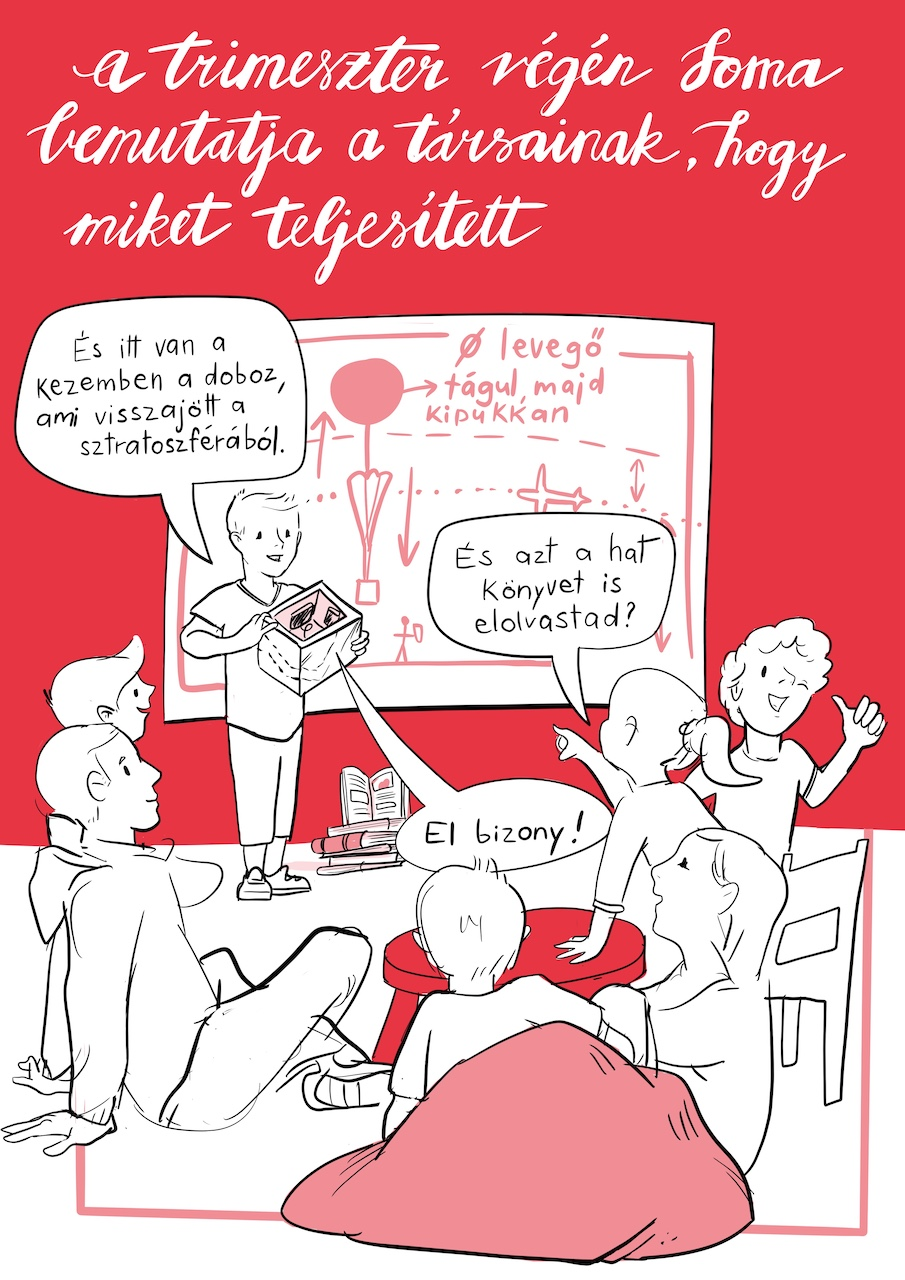
\includegraphics{pics/4a_portfolio_soma.jpg}
\caption{Portfólió  tartalmazza a gyerek által elvégzett feladatokat,
projekteket, alkotásait.}
\end{figure}

A portfólió folyamatosan frissül, a mindennapi, formális, nem-for\-má\-lis
és informális tanulási helyzetek bármikor adhatnak okot a portfólió
frissítésére. Az iskola életében kiemelt szerepe van a következő
eseményeknek.

Minden \emph{modul végeztével} a portfólióba kerül:

\begin{enumerate}
\def\labelenumi{\arabic{enumi}.}
\tightlist
\item
  A képesség elsajátításának, tanulási eredmény elérésének a ténye. Ha a
  modul során a gyerek megtanult százas számkörben alapműveleteket
  végezni, akkor annyi kerül be a portfólióba, hogy „\emph{Szóban és
  írásban összead, kivon, szoroz és oszt a százas számkörben}''.
  Amennyiben a készséget-képességet a gyerek és a tanár megítélése
  alapján nem sikerült megfelelően elsajátítani, úgy a gyakorlás ténye
  kerül be a portfólióba.
\item
  Az alkotás vagy a projektmunka eredménye, ha a modul célja egy alkotás
  létrehozása volt.
\item
  A részvétel ténye, ha a jelenlét volt a modul célja (például
  kirándulás az Országos Kéktúra útvonalán).
\item
  Az elvégzett vizsgák, tudáspróbák, képességfelmérők, diagnózisok
  eredményei tanulási eredmények igazolásával is járnak.
\item
  A \emph{kipakolás} célja, hogy a gyerekek a tanároknak, szülőknek és
  más érintetteknek bemutassák elvégzett munkájukat, azaz a
  portfólióváltozásukat. A kipakolásra való felkészülés tulajdonképpen a
  portfólió összeállítása, prezentálásra való felkészítése, a
  \emph{portfólió frissítése}.
\item
  Társas visszajelzés eredményeként minden gyerek kap visszajelzést a
  társaitól. Ilyenkor összegyűjtik, mit tett a gyerek, ami a többiek
  elismerését és háláját kivívta. Ez is releváns adatokkal szolgálhat a
  portfólióhoz.
\item
  A gyerek saját értékelése, reflexiója arról, hogyan értékeli, amit
  elért, fontos eleme a portfóliónak.
\item
  A tanárok adhatnak kompetenciatanúsítványokat. Ezek rövid, specifikus
  visszajelzések, amelyek mutatják, ha valamit a gyerek megcsinált,
  valamiben fejlődött.
\end{enumerate}

A mentorok segítenek a gyerekeknek a tanulás módját, folyamatát és
eredményeit bemutatni portfólióban.

\begin{figure}
\centering
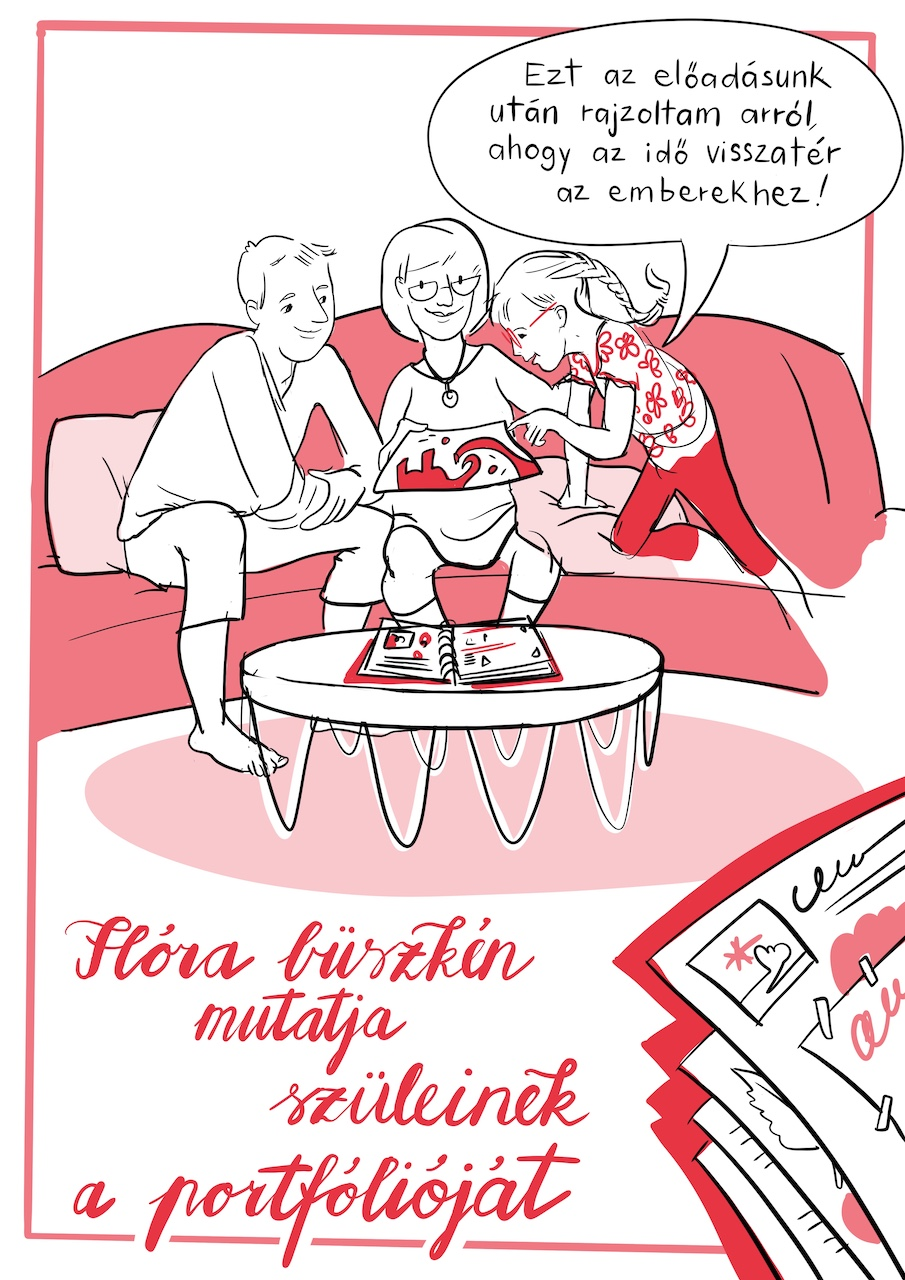
\includegraphics{pics/4b_portfolio_flora.jpg}
\caption{A portfólió segíti, hogy a szülők is jobban tudják követni a gyerekük tanulását, fejlődését. }
\end{figure}

\hypertarget{formai-kovetelmenyek}{%
\paragraph{Formai követelmények}\label{formai-kovetelmenyek}}

A portfóliónak rendezettnek, hozzáférhetőnek, elérhetőnek,
visszakereshetőnek és könnyen bővíthetőnek kell lennie.
A tanulóközösségeknek 
olyan
(technológiai) megoldást kell választaniuk,\break
aminek
alapján a gyerek, tanár és a szülő \emph{naponta} tudja a portfóliót
bővíteni, és akár \emph{heti rendszerességgel} át tudják tekinteni
időrendben, modulonként vagy tantárgyanként a portfólió bővülését.

\hypertarget{a-tanev-ritmusa}{%
\section{A tanév ritmusa}\label{a-tanev-ritmusa}}

A tanév több ciklus ismétlődésével írható le. A személyre szabott, saját
célok által irányított tanulást a trimeszterek ciklusa határozza meg, az
iskolarendszerben megszokott értékeléseket és bizonyítványokat a féléves
ciklus határozza meg. Miért vezeti be az iskola a trimesztereket? Hogy
tanévenként kétszer szánjunk minőségi időt arra, hogy a gyerekek
ránézzenek a tanulási útjaikra, ha kell, tervezzenek újra, és kapjanak új lendületet.


\hypertarget{trimeszterek}{%
\subsection{Trimeszterek}\label{trimeszterek}}

A tanév tanulási útját három szakaszra bontja az iskola, ezeket három
mérföldkő zárja le. Ezeket az időszakokat hívjuk \emph{trimesztereknek}.
Egy trimeszteren belül a tanulási célok tervezése után következik a
tanulás, és a ciklust a visszajelzés és értékelés zárja. Amint egy
ciklus véget ér, elkezdődik egy új.

Ez a felosztás követi az üzleti világ negyedéves tervezését, néhány
egyetem trimeszterekre bontását, de leginkább az évszakokat. Minden
periódus után értékeljük az elmúlt három hónapot, ünnepeljük az
eredményeket, és megtervezzük a következő időszakot.

Az egyes trimeszterek átlagosan 12 hétig tartanak úgy, hogy a tanítással
eltöltött napokat és a tanítási szüneteket mindig az állami oktatásirányítás
által kiadott tanév rendjéhez igazodva határozzuk meg. A trimeszterek
első hete mindig a tervezéssel, utolsó hete mindig az értékeléssel
telik. Trimeszterenként átlagosan további egy hét a közösség építésével,
önálló tanulással zajlik.

A trimesztereken belül az egyes tanulóközösségek között lehetnek néhány
hetes eltérések, melyek a közösség sajátosságait követik.

A ciklusok állandósága adja a tanulás irányításához szükséges kereteket.
Ezek megtartásáért az egyes tanulóközösségek tanulásszervezői felelnek,
működésüket a fenntartó monitorozza. A tanév ritmusát, a
trimeszteralapú tervezés és a félévalapú iskolarendszer-szintű
visszajelzés illeszkedését a következő táblázat mutatja.

\begin{longtable}[]{@{}ll@{}}
\toprule
időszak & Tevékenység\tabularnewline
\midrule
\endhead
Szeptember & közösségépítés\tabularnewline
& saját célok meghatározása\tabularnewline
& modulok kialakítása és meghirdetése\tabularnewline
Október & tanulás, alkotás\tabularnewline
November & tanulás, alkotás\tabularnewline
December & portfólió frissítése\tabularnewline
& reflexiók\tabularnewline
& visszajelzések\tabularnewline
& célok felülvizsgálata\tabularnewline
& modulok változtatása igény esetén\tabularnewline
Január & tanulás, alkotás\tabularnewline
& féléves értékelés kiadása\tabularnewline
Február & tanulás, alkotás\tabularnewline
Március & portfólió frissítése\tabularnewline
& reflexiók\tabularnewline
& visszajelzések\tabularnewline
& célok felülvizsgálata\tabularnewline
& modulok változtatása igény esetén\tabularnewline
Április & tanulás, alkotás\tabularnewline
Május & tanulás, alkotás\tabularnewline
Fél június & évzárás, értékelés, bizonyítványok\tabularnewline
\bottomrule
\end{longtable}

\hypertarget{feleves-es-evvegi-ertekeles}{%
\subsection{Féléves és évvégi
értékelés}\label{feleves-es-evvegi-ertekeles}}

A külső rendszereknek és a törvényeknek való megfelelés miatt az iskola
(az ötödik évfolyamtól) két félévre bontva határozza meg a
tananyagtartalmakat, és ezzel összhangban az iskola automatikusan félévenkénti értékelést
állít ki a portfólió alapján, ami nem más, mint a
portfólióba bekerült értékelések összegyűjtése.

A félév vége január vége (amit egy miniszteri rendelet évente határoz
meg), ami a második trimeszterbe esik, ezért a féléves értékelést az
első trimeszter végén rögzített állapot szerint adja ki az iskola. Az
5--12. évfolyamon lévő gyerekeknek januárban módjuk és lehetőségük van a
portfóliójuk frissítésére, ha a féléves értékelés és az osztályzatokra
váltás eredménye számukra iskolaváltás, továbbtanulás miatt vagy egyéb okból
fontos. Ilyenkor januárban alkalmuk van javítani, ha 
továbbtanulás miatt szükségük van osztályzatokra. Részletesebben az
évfolyamokról, osztályzatokról, bizonyítványokról szóló fejezet (\ref{evfolyam-osztalyzatok-bizonyitvany}.~fejezet, \pageref{evfolyam-osztalyzatok-bizonyitvany}.~oldal)
határozza meg a folyamatot.

Év végén, június hónap fele marad az évvégi zárásokra és igény szerint az
osztályzatokra váltásra való felkészülésre, ami a portfólió frissítését,
bővítését, kiegészítését jelenti.

\hypertarget{visszajelzes-ertekeles}{%
\section{Visszajelzés, értékelés}\label{visszajelzes-ertekeles}}

Ahhoz, hogy hatékony legyen a tanulás, fejlődés, fontos, hogy a
gyerekek, tanárok és szülők is tudják, hogy

\begin{enumerate}
\def\labelenumi{\arabic{enumi}.}
\tightlist
\item
  hol tart most a gyerek, mit tud most,
\item
  hova akar vagy kell eljutni, azaz, mi a célja,
\item
  mi kell ahhoz, hogy elérje a célját.
\end{enumerate}

Ezek mellett mindenkinek hinnie kell abban, hogy odafigyeléssel,
gyakorlással a gyerek meg tud tanulni egy konkrét dolgot. Fontos, hogy
magas legyen a gyerekek énhatékonysága, erős legyen az önbizalmuk, és
nem szabad félniük a hibázástól, a nem-tudástól, mert a tanulás első
lépése, hogy elfogadjuk, hogy valamit nem tudunk. Azaz fontos, hogy
fejlődésfókuszú legyen a gondolkodásuk (growth mindset) {\autocite{Dweck2006}}, azaz

\begin{enumerate}
\def\labelenumi{\arabic{enumi}.}
\setcounter{enumi}{3}
\tightlist
\item
  hinniük kell, hogy el tudják érni a céljukat.
\end{enumerate}

A visszajelzés, értékelés akkor jó és hasznos, azaz hatékony, ha ebben
a négy dologban segít. Mai tudásunk szerint ehhez:

\begin{itemize}
\item
  Rendszeresen visszajelzést kell kapniuk és adniuk.
\item
  A tanulási céloknak és visszajelzéseknek minél specifikusabbaknak kell
  lenniük azaz például ne a 8. osztályos \emph{matematikatudást}
  értékeljük, hanem hogy mennyire képes valaki \emph{fagráfokat
  használni feladatmegoldások során}. (Ez a konkrét példa a matematika
  tantárgy egyik tanulási eredménye.)
\item
  A \emph{„hol tartok most''} diagnózisnak mindig cselekvésre,
  viselkedésre kell vonatkoznia. Ne az legyen a visszajelzés, hogy
  \emph{„ügyes vagy egyenletekből''}, hanem hogy {„gyorsan és pontosan
  oldottad meg a 4 egyenletet''}. A legjobb, amikor a visszajelzés
  konkrét megfigyelésen alapul, és tudni, hogy mikor, hol történt az
  eset: \emph{„amikor társaiddal Minecraftban házat építettél, akkor
  pontosan kiszámoltad a ház területét''.}
\item
  Ha a cél nem a mások legyőzése, akkor a visszajelzés se tartalmazzon
  olyan állítást, ami másokkal való összehasonlítást tartalmaz (így kerüljük a \emph{tehetség}
  szót is, aminek bevett definíciója szerint az átlagnál jobb képesség).
  A mások szintjéhez hasonlított szint felmérése akkor (és csak akkor) fontos, amikor a
  cél egy versenyszituációban jó eredményt elérni.
\item
  A gyerek legyen részese a visszajelzésnek, ő is értékelje saját
  munkáját. Így fejlődik a
  % \href{https://educationendowmentfoundation.org.uk/public/files/Publications/Metacognition/EEF_Metacognition_and_self-regulated_learning.pdf}
  {\emph{metakogníciója}} {\autocite{eef:18}}.
  Értse, tudja, hogy miért és mire vonatkozik a visszajelzés.
\item
  A visszajelzésnek transzparensen hatással kell lennie a
  tanulásszervezésre. Legyen része a folyamatnak, és a gyerek, a tanár és
  a szülő is értse, hogy a visszajelzés alapján mit és hogyan csinálunk
  másképp.
\end{itemize}

\hypertarget{tobbszintu-visszajelzes}{%
\subsection{Többszintű visszajelzés}\label{tobbszintu-visszajelzes}}

A Budapest School-iskolákban a gyerekek többféle visszajelzést kapnak.

\begin{enumerate}
\def\labelenumi{\arabic{enumi}.}
\item
  Minden modul elvégzése után a modul céljai, témája, fókusza alapján a
  gyerekek visszajelzést kapnak a tanulásukról, alkotásaikról,
  eredményeikről, fejlődésükről és viselkedésükről.
\item
  Trimeszterenként a gyerekek visszajelzést kapnak arról, hogy
  általában hogyan haladtak a tanulási célok felé.
\item
  Ennek része, hogy a tantárgyi tanulási eredmények alapján hogyan
  haladt a gyerek a tantárgyakhoz tartozó követelmények teljesítésében.
  Ennek részletes leírását az
  ,,évfolyamok, osztályzatok, bizonyítvány'' fejezet (\ref{evfolyam-osztalyzatok-bizonyitvany}.~fejezet, \pageref{evfolyam-osztalyzatok-bizonyitvany}.~oldal) tárgyalja.
\item
  Szintén legalább trimeszterenként a gyerekek arról is kapnak
  visszajelzést, hogyan működnek a közösségben.
\end{enumerate}

\hypertarget{az-ertekelo-tablazatok}{%
\subsection{Az értékelő táblázatok}\label{az-ertekelo-tablazatok}}

A Budapest School visszajelzéseinek sokkal részletesebbeknek kell
lenniük, mint azt a tantárgyi érdemjegyek és osztályzatok lehetővé
teszik, ezért az érdemjegyek helyett a iskola értékelő táblázatokat
(angolul rubric) alkalmaz. Az értékelő táblázatban szerepelnek az
értékelés szempontjai és a szempontonkénti szintek, rövid leírásokkal.
Ezek alapján a gyerekek maguk is láthatják, hogy hol tartanak, hogyan
javíthatnak még a munkájukon. A táblázatok formája minden visszajelzés
esetén (értsd: modulonként, célonként) változtatható.

\hypertarget{ertekeles-nyelvezete}{%
\subsection{Az értékelés nyelvezete}\label{ertekeles-nyelvezete}}

Fontos alapelv, hogy minél inkább a folyamatot, cselekvést jutalmazzuk,
értékeljük. Tehát arra fókuszáljunk, hogy \emph{mit csinált} a gyerek,
és ne arra, hogy \emph{milyen} a gyerek. Azokra a viselkedésmintákra
adjunk megerősítő visszajelzést, amelyeket látni szeretnénk a gyerekben
később. Lehetőleg kerüljük a statikus jellemzőkre, személyiségjegyekre
vonatkozó értékelést. Így nem azt mondjuk, hogy \emph{„mindig jó vagy
matekból''}, hanem, hogy \emph{„kitartóan és odafigyelve oldottad meg a
feladatot''}.

Álljon itt néhány példa cselekvésre vonatkozó visszajelzésre.

\begin{itemize}
\tightlist
\item
  Fantasztikus, ma egy nagy kihívást választottál!
\item
  Bátran vállaltad a rizikót!
\item
  Nagyon jó! Tényleg sokat próbálgattad.
\item
  Kitartóan csináltad, erre nagyon büszke vagyok!
\item
  De jó, valami újat próbáltál ki ma!
\item
  Köszönöm, hogy ma valakinek segítettél.
\item
  Nagyon nagy öröm látni a haladásodat!
\item
  Ne feledd, mindannyian tudunk a hibáinkból tanulni. Örüljünk annak,
  hogy ma valamit jobban tudunk, mint előtte.
\item
  Hú, egy nehéz feladatot oldottál meg!
\item
  Szép munka! Kipróbáltál egy másik módszert.
\end{itemize}

Az iskolában történő folyamatos visszajelzés a mindennapok része.

\chapter{Hogyan szervezzük az iskolát}
\hypertarget{biztonsagos-tanulasi-kornyezet}{%
\section{Biztonságos tanulási
környezet}\label{biztonsagos-tanulasi-kornyezet}}

A közösség minden tagja számára biztonságos és kiegyensúlyozott
környezet kialakításáért és fenntartásáért a tanulásszervező tanárok a
felelősek.

A Budapest School a tanulásszervezés folyamatait folyamatosan fejleszti.
A folyamatok kialakításakor és fejlesztésekor a legfontosabb szempontok
a következők:

\begin{enumerate}
\def\labelenumi{\arabic{enumi}.}
\item
  A legfontosabb az, hogy a tanulás és az iskolában eltöltött idő mindenki
  számára legyen biztonságos, fizikai és érzelmi szempontból egyaránt.
\item
  Egyensúlyban kell tartani az iskola tagjainak egyéni fejlődését és
  tanulását, és a közösség tagjainak együttműködését, kapcsolódását.
\end{enumerate}

Ez azt is jelenti, hogy nem tartható fenn az az állapot, amikor a
közösség egyik tagjának érdekei felülírják a többiek érdekeit, ahogy az
sem, amikor a közösség valakinek az igényeit nem veszi figyelembe, vagy
amikor a közösségi kapcsolódás felülírja a tanulási célokat.

\vspace*{.5ex}
\hypertarget{szervezet-architekturaja}{%
\section{A szervezet architektúrája}\label{szervezet-architekturaja}}

Az iskolák hagyományosan hierarchikus vezetési és munkaszervezési
elveket követnek. Főnök---beosztott viszonyok, felülről jövő döntések és
autoritás határozza meg a mindennapi folyamatokat. Az állandóság és a
biztos siker érdekében ezek az iskolák a centralizált hatalmat
alkalmazzák: a főnök dönt, a beosztottak végrehajtanak. A Budapest
School a mai világra reflektálva egy dinamikusabb, gyors változásokat
támogató modellt dolgozott ki az egyes tanulóközösségek hatékony és
mégis decentralizált működtetésére.

Olyan kihívásokra reflektál ez a működési mód, amelyek nagyobb\break
komplexitást, transzparenciát és szélesebb körű kommunikációs
lehetőségeket kívánnak meg. Így rövidülhet a döntéshozatal, a gazdasági,
a környezetet és a tanulás körülményeit érintő kérdésekben pedig
növekszik az érintettek felhatalmazása és bevonódása. A Budapest School
egy olyan modell működtetését határozza meg, amely önfenntartó,
környezettudatos és etikus. Támogatja a munkavállalók kreativitását és
lelkesedését, és egy agilis, gyorsan változó és fejlődő szervezet
épülését segíti.

\vspace*{.5ex}
\hypertarget{a-budapest-school-szervezeti-modellje-szociokracia}{%
\subsection{A Budapest School szervezeti modellje,
szociokrácia}\label{a-budapest-school-szervezeti-modellje-szociokracia}}

A szociokrácia egy olyan új „szociális technológiát'' biztosít a
szervezetek irányítására és működtetésére, amelyet a hagyományos,
hierarchikus szervezetektől eltérő alapvető szabályok határoznak meg.


A célirányos és változásra fogékony
szervezetek számára kidolgozott öngazdálkodó gyakorlatról van szó.

A megközelítés ---~az ,,agilis'' és a ,,lean'' megoldásokhoz hasonlóan~--- „just in
time'', vagyis épp a kellő pillanatban reagál a felmerülő változásokra és
lehetőségekre. Mindezt pedig a vállalat minden szintjén önállóan teszi.

Az iskolai szervezet alapelemei a következők:
\newpage
\begin{itemize}
\tightlist
\item
  egy keretrendszer, ami lefekteti a „játékszabályokat'', és újraosztja a
  hatalmat,
\item
  egy módszer a szervezet újrastrukturálásához és az emberek szerepeinek
  és önállóságának meghatározásához, és
\item
  egy egyedülálló döntéshozatali folyamat a hagyományos döntési
  folyamatok felfrissítéséhez.
\end{itemize}

\hypertarget{dinamikusan-valtozo-szerepek}{%
\subsection{Dinamikusan változó
szerepek}\label{dinamikusan-valtozo-szerepek}}

A klasszikus iskolában minden alkalmazott rendelkezik egy munkaköri
leírással, mely felsorolja feladatait és hatáskörét. Ez általában a
legkevésbé sincs összhangban a nap mint nap végzett feladatokkal. A
Budapest School iskolában a dolgozók gyakran számos szereppel
rendelkeznek, és ezeket akár teljesen különböző
munkacsapatokon belül is betölthetik. A szerepek folyamatos alakuláson mennek
keresztül, és a csapat résztvevői frissítik őket. A szerepkörök tehát
nincsenek szorosan egy emberhez kötve: mindig az látja majd el, aki
ért hozzá, van szabad kapacitása és elvállalja. Ezzel pedig sok
személyes konfliktus kerülhető el.

Ahogy például \emph{a fociban is
pontosan tudod, hogy a labdát a csatárnak kell passzolnod}. Nem azért, mert jóban vagytok, hanem mert ő van a legjobb helyzetben,
hogy gólt lőjön a csapatnak. Még ha nem is vagy vele jóban, nem kedveled
vagy ki nem állhatod, akkor is neki fogsz passzolni, mert a játék
stratégiája szerint így kell tenned. Ugyanígy az iskolánkban az egyes
szerepek rendelkeznek hatalommal, nem pedig a személyek. Ez azt is
jelenti, hogy a szerepek és a hatalom állandóan változhatnak anélkül,
hogy a játékszabályokat megsértenénk. Nincs állandó főnök---beosztott
viszony.

\hypertarget{szetosztott-hatalom}{%
\subsection{Szétosztott hatalom}\label{szetosztott-hatalom}}

A hagyományos iskolai struktúrában az igazgató és a vezetőség tagjai nem
delegálnak hatalmat. Minden döntés átmegy az ő kezeiken. A
Budapest School-iskolában a hatalmat ténylegesen elosztjuk, így a
hierarchia helyett egymással kapcsolatban lévő és kommunikáló, de
önállóan döntő csapatok (úgynevezett körök) a döntéshozók. A körök
közötti kapcsolat jelentősen meg tudja növelni az iskola alkalmazkodóképességét.

\hypertarget{allando-tyuklepesek}{%
\subsection{Állandó tyúklépések}\label{allando-tyuklepesek}}

Budapest School-iskolában a szervezeti struktúrát minden hónapban
felülvizsgálhatják: megvizsgálják, hogy az adott szerepek milyen
feladatokkal és döntésekkel járnak. A változások tömérdek apró lépésben
történnek, szünet nélkül, folyamatosan. Így a csapat kihasználhatja a
lehetőségeket, hogy tanuljon az esetleges hibákból, fejlessze önmagát, és
tökéletesítse a folyamatokat. Ahogy Alexis Gonzales-Black, a Zappos
munkatársa mondja (ez a cég talán a legelsők között csatlakozott a
,,holakrácia'' nevű rendszernek a valóságba való
átültetéséhez), „a holakrácia nem fogja megoldani helyetted a
problémáidat; viszont jó eszköz arra, hogy te saját magad megoldhasd őket.''

\hypertarget{mindenki-szamara-atlathato-szerepek}{%
\subsection{Mindenki számára átlátható
szerepek}\label{mindenki-szamara-atlathato-szerepek}}

„Mi mindig így csináljuk'' --- hangzik el számos iskolában a válasz, hogy
ez vagy az miért éppen így történik. Gyakran senki sem tudja, hogy az
adott szabály miért létezik, mi célt szolgál, ki döntött róla, vagy ki
tudná megváltoztatni. Ez pedig a hatalom szétosztását lehetetlenné
teszi. A Budapest School iskolában
\emph{a hatalom nem a csoport élén álló vezetők kezében van,}
hanem az expliciten definiált folyamatokhoz kötődik. Ezek a
„játékszabályok'' mindenki számára elérhetők és ismertek, legyen szó
akár régi motorosokról, akár újoncokról.

A Budapest School modellel tehát nem káoszt és hatalmi játszmákat
generálunk, hanem
\emph{eltöröljük a hagyományos hierarchiából fakadó lassú folyamatokat,}
az átláthatatlan felelősségi köröket, és szabad utat engedünk a
kreativitásnak, az önállóságnak. Azáltal, hogy felhatalmazza az
embereket arra, hogy értelmes döntéseket hozhassanak, és részt vehessenek
a változásban, a holakrácia felszabadítja a szervezet kihasználatlan
erőforrásait.

\hypertarget{az-iskola-kormanyzasa}{%
\section{Az iskola kormányzása}\label{az-iskola-kormanyzasa}}

Az iskola szervezetét a tagjai együtt alakítják. A szervezet élő,
folyamatosan változik, a következő alapelvek mentén:

\begin{itemize}
\tightlist
\item
  Gyorsan és folyamatosan tanuló, agilis szervezetként az iskola
  mindennap jobban támogatja a gyerekek tanulását, mint az előző napon.
\item
  Minden résztvevőnek a stabilitás, biztonság, kiszámíthatóság iránti igénye
  pont annyira fontos, mint a változás, a javulás, a fejlődés igénye.
\item
  A gyerekeket leginkább ismerő, a hozzájuk legközelebb álló tanárok
  (a gyerekekkel és a szülőkkel erős kapcsolatban) minél több helyzetben
  hoznak döntéseket.
\item
  Állandó az együttműködés, a partneri kapcsolat, a kölcsönös
  felhatalmazás
  nem csak a tanár---gyerek kapcsolatban,
  hanem a tanárok és adminisztrátorok között is.
\end{itemize}

Azt szeretnénk, hogy gyerekeink kreatív, környezetüket aktívan alakító,
mély partneri kapcsolatokban élő, problémamegoldó, csapatjátékos,
folyamatosan tanuló, a világot változtatni tudó felnőttekké váljanak.
Ehhez olyan iskolát építünk, ahol a tanárok kreatívak, környezetüket
aktívan alakítják, mély partneri kapcsolatban élnek, problémákat oldanak
meg, csapatban dolgoznak, és folyamatosan tanulnak.

Az iskolát mint szervezetet a \emph{szociokrácia}
szervezeti modellje alapján működtetjük, mert így tudjuk leginkább elérni,
hogy az együttműködésünk egyszerre legyen
örömteli és hatékony. Ez egy
olyan, az üzleti világban is kipróbált dinamikus döntéshozatali
rendszer, amely egyszerre segíti a harmonikus és örömteli közösségi
együttműködést, és jelent garanciát arra, hogy az együttműködés hatékony
lesz az egyes csapatokon belül.

\hypertarget{donteshozas}{%
\subsection{Döntéshozás}\label{donteshozas}}

Az iskola minden csapata (a tanulócsoportokat vezető tanulásszervezők,
a gyerekek egy csapata stb.) a \emph{hozzájáruláson alapuló döntési
mechanizmust} (consent based decision making) használja ahhoz, hogy a
szervezet gyorsan tudjon döntést hozni, \emph{és} minden tagja
hallathassa a hangját.

A csapat valamennyi tagja tehet javaslatokat, ha nem hatékony működést,
feszültséget, problémát észlel, és van rá megoldása. A javaslat
értelmezése után az érintettek mindegyikét meg kell hallgatni, hogy
\emph{elfogadhatónak} tartja-e a javaslatot, azaz hozzájárul-e a
változáshoz, mert \emph{„elég jónak és biztonságosnak találja, hogy
kipróbáljuk az új működést”} (\emph{,,is this good enough for now and
safe enough to try?''}). Fontos, hogy mindenki egyenként hallassa
a hangját. A javaslatot akkor tekintjük elfogadottnak, ha és amikor minden érintett
hozzájárult.

Mindenki kifejezheti a \emph{fenntartásait} (concern), és a csapat
feladata ezeket meghallani, és reagálni rájuk. A fenntartás azonban még
nem jelenti a javaslat elutasítását, csak fontos információt ad a döntés
végrehajtásához.

A javaslatot a csapat nem fogadja el, ha valamelyik csapattag
\emph{ellenzi} azt (objection). Az ellenzés egy én-üzenet, valami
ilyesmi: „ha a csapat ezt a döntést meghozná, akkor mélyen sérülne a
csapathoz való elköteleződésem, mert az én igényemet, ami~\ldots{}, nem
elégíti ki a javaslat. Nekem szükségem van~\ldots{}, ezért inkább
javaslom, hogy~\ldots{}''. Fontos, hogy az ellenvetést megfogalmazó
mondja el a saját igényeit, szükségleteit és tegyen új javaslatot, vagy
kérjen segítséget, hogy milyen új javaslatot tehetne. Ellenvetés esetén
a csapat együtt dolgozik azon, hogy új javaslatot találjon, ami az
ellenvetést feloldja, és az eredeti javaslat célja felé viszi a
szervezetet.

\hypertarget{a-hozzajarulas-nem-konszenzus}{%
\paragraph{A hozzájárulás nem
konszenzus}\label{a-hozzajarulas-nem-konszenzus}}

A konszenzusalapú döntések esetében mindenkinek egyet kell értenie abban,
hogy a döntés a legjobb, leghelyesebb, leghelyénvalóbb. A Budapest
School iskolában azt a kérdést tesszük fel inkább, hogy van-e valakinek
ellenvetése és a javaslat kellően biz\-ton\-sá\-gos-e ahhoz, hogy kipróbáljuk.
Nem azt a kérdést tesszük fel, hogy mindenki ezt a döntést hozta volna-e,
és hogy mindenki egyetért-e a döntéssel, hanem azt, hogy mindenki tudja-e
támogatni a csapat egy másik tagját, és hogy nincs-e olyan ismert kockázat,
ami az egyén vagy a szervezet szempontjából nem vállalható.

\hypertarget{a-hozzajarulas-nem-szavazas}{%
\paragraph{A hozzájárulás nem
szavazás}\label{a-hozzajarulas-nem-szavazas}}

A Budapest School-iskolában nem a többség dönt, és nem az számít, hogy
hányan akarnak egy döntés mellé állni. Mindenki hozhat döntést, amit
elfogad a csapat minden tagja, azaz egyetlenegy ellenvetés sincs.

\hypertarget{az-ellenvetes-nem-veto}{%
\paragraph{Az ellenvetés nem vétó}\label{az-ellenvetes-nem-veto}}

A vétójog a döntés megakadályozását jelenti. Amikor valaki
megvétóz egy döntést, akkor azzal a folyamat általában megakad. Az
iskola működésében használt ellenvetés egy beszélgetés megindítását
jelenti: „ezt én így nem tudom támogatni, helyette ezt javaslom inkább''.

\hypertarget{a-van-egy-jobb-otletem-nem-ellenvetes}{%
\paragraph{A „van egy jobb ötletem'' nem
ellenvetés}\label{a-van-egy-jobb-otletem-nem-ellenvetes}}

A szervezetnek nem az a feladata, hogy a legjobb döntéseket hozza, hanem
hogy amikor szükséges, akkor javítson a működésén. Ezért minden
döntéskor mindenkinek azt kell mérlegelnie először, hogy elfogadható-e
neki, hogy azt a bizonyos javaslatot kipróbálja a csapat. Attól, hogy
valaki jobb, más javaslatot is tud, attól még először az eredeti
javaslatot érdemes kipróbálni és tesztelni.

\hypertarget{minden-javaslat-csak-egy-hipotezis}{%
\paragraph{Minden javaslat csak egy
hipotézis}\label{minden-javaslat-csak-egy-hipotezis}}

Amikor valamit változtatunk a szervezet működésén, akkor egy kísérletbe
vágunk bele: kipróbáljuk, hogy az új működés tényleg jobb-e, megoldja-e
a problémát, feszültséget, ki\-e\-lé\-gí\-ti-e az igényeket. A döntés
támogatásakor ezt a próbálkozást támogatjuk.

\hypertarget{nem-dontunk-mindenrol-egyutt}{%
\paragraph{Nem döntünk mindenről
együtt}\label{nem-dontunk-mindenrol-egyutt}}

A Budapest School-iskolában csak az iskola és a tanulóközösség működését
megváltoztató kormányzási kérdésekről döntünk együtt.~A Budapest School
minden tagja szerepeiből kifolyólag fel van hatalmazva arra, hogy a
mindennapi döntéseit maga meghozhassa, ezért nem kell mindent
megbeszélnünk. A cél, hogy olyan szerepeket és rendszereket alakítsunk
ki, hogy a mindennapi döntéseket mindenki maga meg tudja hozni.

\hypertarget{csapatok-az-iskola-szervezeti-egysegei}{%
\subsection{Csapatok --- az iskola szervezeti
egységei}\label{csapatok-az-iskola-szervezeti-egysegei}}

A Budapest School csapatai (a szociokrácia terminológiájában a
\emph{körök}) önálló csoportok egy jól meghatározott céllal, felruházott
felelősséggel, döntési körrel. A csapatok maguk határozzák meg a saját
működésüket (policy making), és végzik el a saját feladatukat. Az
iskolában azok döntenek együtt, akik együtt dolgoznak, egy csapatban
(,,those who associate together govern together''). És fontos, hogy akik
együtt dolgoznak, jól legyenek egymással.

Azt is tudjuk, hogy akik egy munkát elvégeznek, azok a munka szakértői,
ezért ők tudnak arról a legjobban dönteni, hogy hogyan érdemes a
munkájukat szervezni, alakítani. Nincs főnök, külső szakértő, aki
megmondja egy csapatnak, mit és hogyan csináljanak addig, amíg a rájuk
felhatalmazott kereteken belül maradnak. Az természetes, hogy minden
segítséget, támogatást, információt megkapnak, amire szükségük van. De a
kormányzás az ő kezükben van.

\hypertarget{tanulokozossegek-tanulasszervezo-csapata}{%
\paragraph{Tanulóközösségek tanulásszervező
csapata}\label{tanulokozossegek-tanulasszervezo-csapata}}

A Budapest School szervezet állandó csapatai az egy-egy tanulóközösséget
vezető tanulásszervezők csapata, ami egy \emph{szociokratikus kör}. A
tanulóközösség gyerekeinek (családjainak) és tanárainak életét
meghatározó döntéseket maguk hozzák\break
meg. Így például a napirend, a
csoportbontások, a szülői értekezletek tematikája a saját döntéseik
alapján alakul ki. Fontos, hogy a csapattagok maguk tudják meghatározni,
kivel tudnak és akarnak együtt dolgozni, mikor és mit akarnak csinálni.

\hypertarget{csapatok-kapcsolodasa}{%
\paragraph{Csapatok kapcsolódása}\label{csapatok-kapcsolodasa}}

Egy-egy ember több csapatnak is tagja lehet. Egyrészt munkacsoportok
alakulhatnak egy-egy feladat elvégzésére, és a Budapest Schoolban egy
ember több részfeladatot is ellát. Másrészt a csapatokat kifejezetten
úgy alakítja a közösség, hogy legyenek köztük kapcsolódások, olyan
tagok, akik összekötik a csapatokat.

Vannak olyan csapatok, melyek elsődleges célja összekötni a kisebb
csapatokat. Például minden tanulóközösség tanárcsapata delegál egy
képviselőt az iskola közös naptárát létrehozó munkacsoportba.

\hypertarget{csapatok-vezetoi}{%
\paragraph{Csapatok vezetői}\label{csapatok-vezetoi}}

Minden csapatnak van egy \emph{vezetője} (a szociokrácia\break
terminológiájában a
\emph{circle leader}). A vezető feladata, hogy mindenki ismerje a csapat
célját, a választ a \emph{„miért létezünk?''} kérdésre, és hogy a csapat
működjön: tiszták legyenek a szerepek, és megtörténjen az, amiben
a csapat megállapodott, működjenek és fejlődjenek a folyamatok.

A Budapest School rendszerében a csapat vezetője nem az az ember, aki megmondja,
ki mit csináljon; nem osztja, ellenőrzi vagy felügyeli a feladatokat,
nem rúg ki, és nem vesz fel embereket, hanem szolgálja a csapatot
(servant leadership) azzal, hogy segíti a megállapodásokat betartani:
facilitál, moderál, szintetizál, kísér, kérdez. A csapatvezető
megválasztásához, mint minden szerep megválasztásához, a csapat minden
tagjának hozzájárulása szükséges.

\hypertarget{mi-van-amikor-egy-csapat-nem-tud-dontest-hozni-egyuttmukodni}{%
\subsection{Mi van, amikor egy csapat nem tud döntést hozni,
együttműködni}\label{mi-van-amikor-egy-csapat-nem-tud-dontest-hozni-egyuttmukodni}}

Amikor a csapattagok úgy érzik, hogy nem tudnak mindenki számára
elfogadható döntéseket hozni, nem haladnak, vagy megjelentek a játszmák,
és ezért már nem tudják a csapat célját szolgálni, akkor konfliktus,
feszültség alakul ki, aminek feloldásához segítséget hívhatnak be a
szervezet töb-\break
bi részétől.

A csapat folyamatos harmóniájáért folyamatosan dolgozni kell, ahogy az
egészségünk megőrzésének és a problémák megelőzésének is napi rutinná kell
válnia. Ezért a Budapest School csapatainak erősen ajánlott a
rendszeres visszajelzés, visszatekintés (retrospektív) és a team
coaching.

\hypertarget{operator-a-tanulokozossegek-alapitoja}{%
\section{Operátor, a tanulóközösségek
alapítója}\label{operator-a-tanulokozossegek-alapitoja}}

Vannak tanulóközösségek, amik szervezését, indítását egy \emph{alapító}
\emph{operátor} vagy \emph{operátorcsapat} kezdte el. Az operátorok a
létrehozók, az alkotók, az alapítók, akik minden nehézséget leküzdve a
semmiből létrehoznak egy önállóan működni képes tanulóközösséget.
Nélkülük biztos nem jött volna létre a tanulóközösség.

\hypertarget{az-operator-a-mindenes}{%
\subsection{Az operátor, a mindenes}\label{az-operator-a-mindenes}}

Kezdetben az operátor az egyszemélyes mindenes, hiszen egyedül kezdte a
tanulóközösség tanulás-szervezőjeként. Ő felel a pénzügyekért, a
tanárfelvételért, a csoportbontásokért, a tanulásszervezésért, a szülők
bevonásáért, a gyerekfelvételért és még a mosdókat is ki kell
tisztítani. Már, ha előtte elintéze, hogy legyenek mosdók. Az esetek
többségében ő találja, bérli ki, vagy vásárolja meg, újítja fel a tanuló
közösségnek otthont adó, később telephelyként működő épületet és dönt az
első tanár csatlakozásáról.

Az operátorok aktívak, tesznek, megoldanak, elintéznek, sokszor hirtelen
a Budapest School közösség képviselőjévé válnak.

\hypertarget{az-operator-a-tanulasszervezo-a-tanarcsapat-tagja}{%
\subsection{Az operátor a tanulásszervező, a tanárcsapat
tagja}\label{az-operator-a-tanulasszervezo-a-tanarcsapat-tagja}}

Amikor már megjelennek azok a tanárok, akik a tanulásszervezésért, a
tanulóközösség vezetésért felelnek, tehát a tanulásszervezők (mentorok,
mentortanárok és néhány kiemelt szaktanár), az operátor akkor is a
tanulásszervező csapat része marad. Nem átadja a tanulóközösséget a
tanulásszervezőknek, hanem elkezdik csapatban vezetni a közösséget.
Innentől kezdve a csapat minden tagja, így az operátor és minden
tanulásszervező be van vonva minden döntésbe: mindenki hozzájárulása
szükséges minden, a csapatot és a tanulóközösséget érintő kérdésben.

Ez azt is jelenti, hogy csak olyan döntést fogadhat el a csapat, ami
\emph{mindenkinek} elfogadható, amit mindenki \emph{„elég jónak és
biztonságosnak talál"}. Mindenki mondhatja azt, hogy egy javaslat nem
oké neki, szerinte inkább csinálja a csapat másképp. Ráadásul
javaslatokat mindenki hozhat. Ez azt jelenti, hogy mindenkinek lehet
hatása a működésre.

\begin{quote}
\emph{Példa: Anna, az egyik tanulásszervező javasolja, hogy
délutánonként kisebb csoportokba bontsák a gyerekeket, mert elfáradnak,
és figyelmüket könnyebb lenne úgy megtartani. Ehhez Anna azt javasolja,
hogy bízzanak meg egy külsős szaktanárt, hogy ő tudjon párhuzamosan
művészeti klubot tartani. Péter, a csapat másik tagja kifejezi
ellenvetését, mert épp így is alig van nullán a tanulóközösség, és
inkább tartalékot kéne képezni. Neki szüksége van az anyagi biztonságra.
A csapat megértve Anna és Péter igényeit is, kidolgoz egy olyan
megoldást, ahol extra külsős tanár nélkül is megoldódik az Anna által
felvetett probléma: ha a délutáni foglalkozás előtt időt töltenek az
udvaron, akkor jobban fogják tudni tartani a figyelmet, külön
csoportbontás nélkül is.}
\end{quote}

\hypertarget{az-operator-es-a-csapat}{%
\subsection{Az operátor és a csapat}\label{az-operator-es-a-csapat}}

A szociokrácia rendszerében mindenki vállalhat szerepeket, hatalommal
bíró feladatköröket, ha és amikor erre a csapat felruházza. Ezért az
operátor, aki ugye kezdetben az egyszemélyes mindenes volt,
feladatköröket ad át a többi tanulásszervezőnek. Nagy különbség van
azonban aközött, hogy megkérlek, hogy légy szíves a kirándulásra készíts
össze egészségügyi dobozt, vagy, hogy a csapattal megbeszéljük, hogy van
1. egy balesetvédelmi felelős szerep, amit javasolsz, hogy ezentúl 2. te
végezd el. Az első esetben szívességet kérünk egymástól, a másik esetben
feladatokat, felelősségeket, BPS terminológiában szerepeket adunk át,
delegálunk.

Fontos, hogy a szerepek átadása nem az operátor és az új felelős közti
megállapodás. Ez a csapat életét érintő változtatás, tehát mindenkit be
kell vonni a döntésbe: fontos, hogy mindenkinek elfogadható, hogy
kipróbáljuk, hogy ezentúl ezt a szerepet a javasolt ember viszi tovább?

\begin{quote}
Példa: Anna, egy tanulóközösség operátora sokszor elfelejti kiküldeni a
szülői előtt és után a szülőknek szánt kérdőíveket. Ebből több
konfliktus adódott, mert Péter egy mentor a csapatban, nagyon szeretné
tudni, hogy hogy vannak a szülők. Anna és Péter egy elég komoly vita
(veszekedés?) után vannak. Arra jutottak, hogy inkább Péter felvállalná
a szülői kérdőívek kiküldését és a szülők noszogatását. A következő
tanári meetingen elmondják a javaslatukat, hogy Péter legyen a szülői
visszajelzők kezelője, és kérik a csapatot, hogy Pétertől várják el,
hogy időben kimenjen a levél a visszajelzőkről, és legalább 2
emlékeztetőt küldjön Péter, és legalább egy nappal a szülői előtt
összesítse az eredményeket. Azaz adnak egy pontos szerepdefiníciót, és
javasolják a csapatnak, hogy ezt a szerepet ezentúl Péter vigye. A
csapat minden tagja nagyon örül, mert érezték, hogy ezt a feladatot
érdemes lenne jobban végezni. Kifejezik hálájukat Annának és Péternek,
hogy a nehézségek ellenére fejlesztik a rendszert.\_
\end{quote}

\hypertarget{mi-van-ha-az-operator-nem-akar-vagy-tud-mindenben-reszt-venni}{%
\subsubsection{Mi van, ha az operátor nem akar vagy tud mindenben részt
venni}\label{mi-van-ha-az-operator-nem-akar-vagy-tud-mindenben-reszt-venni}}

Vannak esetek, amikor nem javít a gyerekek tanulási élményén vagy a
tanárok jóllétén, ha az operátor minden döntésben részt vesz, vagy az
operátornak egyéb teendői miatt nincs kapacitása a közösség életében
nagy mértékben részt venni, feladatokat, szerepeket vállalni. Ilyenkor
mondhatja az\emph{t, hogy ``bízom bennetek, szóljatok, amikor úgy
érzitek, hogy kéne róla tudnom. De kérlek titeket, ami a pénzügyeket
érinti, arról szóljatok.''} Sokat kell ilyenkor dolgozni azon, hogy
mindenki tudja, értse és el is találja, hogy mikor kell bevonni az
operátort és mikor nem.

\hypertarget{mi-van-ha-a-tanarokat-nem-erdeklik-a-penzugyek}{%
\subsubsection{Mi van, ha a tanárokat nem érdeklik a
pénzügyek}\label{mi-van-ha-a-tanarokat-nem-erdeklik-a-penzugyek}}

Van, amikor azt érzed, hogy bizonyos dolgokról egyszerűen csak nem
akarsz tudni, csak működjön a dolog. Ilyenkor egyszerűen
felhatalmazhatjuk egymást, hogy egy adott kérdésben légy szíves hozd meg
a döntést, és akár még informálnod sem kell engem. Tanárként azt kérem,
hogy mondd meg, mennyi pénzt költhetek havonta filctollra és
programokra, és most egyelőre nem akarom tudni, hogy a bérleti díj és a
takarítóra költhető keret hogyan függ össze.

A probléma abból eredhet, hogy az operátor először egyedül csinált
mindent, nem volt kivel megbeszélnie a dolgokat. Aztán jöttél te, mint
tanár, és nem akartál mindent megbeszélni, mert sok volt az információ.
Aztán van az a kényelmetlen érzés, hogy szeretnél bevonva lenni, de nem
vagy. Mindenki azt hiszi, hogy ebben megállapodtatok, pedig nem. Csak
történetileg alakult így a helyzet. Ez az a pont, amikor nem az
SZMSZ-hez kell nyúlnod, hanem fel kell hívnod az operátort.

\hypertarget{az-operator-a-tanarcsapat-fonoke}{%
\subsubsection{Az operátor a tanárcsapat
főnöke}\label{az-operator-a-tanarcsapat-fonoke}}

Nem. Ha a főnök azt jelenti, hogy a főnök döntést hoz, a hierarchiában
alatta lévő munkavállalók pedig végrehajtják a döntést, akkor egyértelmű
NEM a válasz. A BPS szervezetek nem így működnek. Az operátor, mint más
is, javaslatokat tesz, és mindenki hozzájárulása esetén a csapat azt
végrehajtja. Ugyanakkor az valószínű, hogy az operátorok habitusuk,
sajátos helyzetük miatt több javaslatot fognak, legalábbis az első pár
évben tenni, mint a többiek.

Minden csapatnak van azonban egy
csapatvezetője (\ref{csapatok-vezetoi}.~fejezet \apageref{csapatok-vezetoi}.~oldalon),
aki azért felel, hogy „a csapat működjön: tiszták legyenek a szerepek és
megtörténjen az, amiben megállapodott a csapat, és működjenek és
fejlődjenek a folyamatok.'' Ahhoz, hogy ezt a célját elérje „facilitál,
moderál, szintetizál, kísér, kérdez.''

Kezdetben ezt a szerepet is az operátor látja el. A csapat dönthet úgy,
hogy ezt a szerepet az operátor átadja egy másik tanulásszervezőnek, aki
ezáltal a csapat koordinátora lesz. Azonban ehhez minden tag
hozzájárulása szükséges. Tehát a BPS-ben nem szavazunk ki senkit, hanem
megbeszéljük, hogy jobb lenne, ha bizonyos szerepet most más végezne.

\hypertarget{az-opertator-felelelosseget-vallal-mindenert}{%
\subsubsection{Az opertátor felelelősséget vállal
mindenért}\label{az-opertator-felelelosseget-vallal-mindenert}}

Nem. Nincs olyan ember a rendszerben, aki mindenért egy személyben
felelős lenne. Egy tornatanár nem felelős minden balesetért, ami
tornaórán történik. Történhet olyan baleset, ami ellen ő nem tudott
volna mit tenni. Azért viszont felelős, hogy ha egyszer már megtanultuk,
hogy balesetveszélyes mélyvízbe ugrania annak, aki nem tud úszni, hogy
megkérdezze mindenkitől, hogy tud-e úszni, mielőtt elkezdődik a
foglalkozás. Ugyanígy: egy operátor/ koordinátor nem felelős azért, hogy
mit csinál egy másik munkatárs, vagy egy gyerek az iskolában, vagy hogy
egy szülő hogyan viselkedik, de azért felelős, hogy ha nem tartunk be
szabályokat és megállapodásokat, akkor tegyen azért, hogy a helyzet
megváltozzon.

\hypertarget{az-operator-kulonleges-szerepe-o-a-penzugyi-stabilitas-biztositoja}{%
\subsection{Az operátor különleges szerepe: ő a pénzügyi stabilitás
biztosítója}\label{az-operator-kulonleges-szerepe-o-a-penzugyi-stabilitas-biztositoja}}

A pénz olyan, mint az oxigén. Szükségünk van rá a tanulóközösség
működtetéséhez. És mivel a Budapest School tanulóközösségek önálló
költségvetéssel bírnak, fontos, hogy egy tanulóközösségnek ne legyen
több a kiadása, mint a bevétele.

Az operátorok által életre hívott tanulóközösségek esetén az operátor
az, aki személyesen felelősséget vállal a pénzügyi stabilitásért. Értsd:
ha többet akar a tanulóközösség költeni, mint a bevétele, akkor neki
kell a zsebébe nyúlni. És ameddig az operátor ezt a felelősséget nem
osztja szét a többi tanulásszervező között (azaz nem szövetkezetként
működnek), addig ő mindig
\_\href{https://en.wikipedia.org/wiki/Primus_inter_pares}{első lesz
az}\_egyenlők között.

\textbf{Akkor ez azt is jelenti, hogy a pénzügyi felelősségvállalás
miatt ő maga meghozhat pénzügyeket érintő döntéseket?} Attól, hogy
operátorként az a dolgod, hogy 1. ne legyen hiány, 2. ha van, akkor
teremtsd elő a hiányt, attól még nem hozol meg minden döntést egyedül.
Mert a ne-legyen-hiány célt sokféleképpen el lehet érni. A csapatnak
kemény munka árán ki kell dolgoznia a saját megállapodásait arról, hogy
mi az a döntés, amire felhatalmazást kaptál.

\hypertarget{az-operator-kilepese}{%
\subsubsection{Az operátor kilépése}\label{az-operator-kilepese}}

Ha konfliktus alakul ki a csoportban, akkor bárki mondhatja azt, hogy
,,én kilépek''. Csak az operátor nem. Vagyis csak nagyon nehezen. Ha
eltűnik az operátor, akkor még az is lehet, hogy megszűnik a
tanulóközösség. Ha mégis olyan helyzet áll elő, hogy kilép, akkor új
operártort kell találni vagy át kell alakítani a struktúrát. Az operátor
ilyenkor is aktívan részt vesz a helyzet megoldásában (pl. az utódja
megtalálásában, az átadás-átvételben, stb).

\hypertarget{koordinator}{%
\subsection{Koordinátor}\label{koordinator}}

Amikor az operátor átadja a csapatvezető szerepet másnak, akkor ezt az
embert koordinátornak kezdjük el hívni, hogy mindenki értse: itt már a
pénzügyi felelősség és a csapatvezetőség szétvált ebben a csapatban. A
koordinátor szintén nem főnök, hanem facilitátor. Sokat gondolkodik
azon, hogy mindenki tudja-e, hogy ki mit és mikor csinál, ő a circle
leader.

Vannak azok a tanulóközösségek, ahol az operátor szerepet a Lab játsza.
Ilyenkor mindig van egy koordinátor a tanulásszervezők között.

\hypertarget{a-kozossegi-let-szabalyai}{%
\section{A közösségi lét szabályai}\label{a-kozossegi-let-szabalyai}}

A Budapest School egy közösségi iskola: a gyerekek együtt tanulnak és
alkotnak, a tanárok csapatokban dolgoznak, és a szülők is egy elfogadó
közösség részének érezhetik magukat. A tagok --- a tanárok, a gyerekek,
a szülők és az adminisztrátorok --- azért csatlakoznak a közösséghez,
mert itt szeretnének lenni, és itt érzik magukat boldognak,
egészségesnek és hasznosnak. A közösség azért fogad be új tagokat, hogy
nagyobb, erősebb közösség lehessen.

\hypertarget{partnerseg}{%
\paragraph{Partnerség}\label{partnerseg}}

A tanulásszervezők és a családok közös célja, hogy közösségük a gyerekek
fejlődését együtt támogassa. A tanulás holisztikus szemlélete révén a
gyerekeknek egyszerre kell jó kapcsolatot ápolniuk saját társaikkal,
partnerségben lenniük tanáraikkal, és meghallaniuk a szülők feléjük irányuló
kéréseit. A tanulás célját a gyerekek maguk határozzák meg, azok az
értékek, rituálék viszont, melyek a mindennapjaikat meghatározzák,
túlmutatnak az egyénen, és a közösség céljait szolgálják oly módon, hogy
az az egyes családok életvitelével is összhangban legyen.

Minden tanulóközösségnek feladata ezért, hogy az együttműködésük, a
közösségi szabályaik, a házirendjük meghatározásakor a családok
véleményét, javaslatait is kikérjék, és úgy hozzanak döntést, hogy az
mindenki számára kellően biztonságos és elég jó döntés legyen.

Ez vonatkozhat a mindennapi eszközök használatára, a közlekedésre, az
együtt, tanulással eltöltött egyéni és csoportos idő arányaira, a
közösen megtartott ünnepekre, jeles napokra, mindazokra a kérdésekre,
melyek közösségi döntések, és hatással lehetnek az egyén fejlődésére.

\hypertarget{alapcsoportok}{%
\paragraph{Alapcsoportok}\label{alapcsoportok}}

A Budapest School iskola kisebb
tanulóközösségekből áll (\ref{a-budapest-school-tanulokozossegei}.~fejezet, \pageref{a-budapest-school-tanulokozossegei}.~oldal). Ez a gyerekek és tanárok elsődleges közössége:
a gyerekek számára ez az a közösség, akikkel együtt járnak iskolába, együtt
alakítják az iskolájukat, a tanárok számára ez az a csapat, akikkel együtt
dolgoznak, hogy létrehozzák, fenntartsák és fejlesszék a tanulóközösség
gyerekeinek tanulási környezetét.

A tanulás egysége a
modul (\ref{tanulasi-tanitasi-egysegek-a-modulok}.~fejezet, \pageref{tanulasi-tanitasi-egysegek-a-modulok}.~oldal).
Egy modul csoportjában a közös érdeklődésű és célú gyerekek tanulnak
együtt, mert együtt boldogabban, hatékonyabban el tudják érni a
céljukat.

\hypertarget{sajat-szabalyok}{%
\paragraph{Saját szabályok}\label{sajat-szabalyok}}

A tanulóközösség és akár egy-egy modul kereteit, szabályait a résztvevők
alakítják ki. Pontosabban a tanárok~felelőssége és feladata, hogy minden
tanár és gyerek számára elfogadható, betartható, releváns és értelmes
szabályok legyenek. (Mikroiskola esetén a tanulásszervező tanárok,
modulok esetén a szaktanárok és a tanulásszervező tanárok közösen.)

Mind a gyerekek, mind a tanárok javasolhatnak új szabályokat vagy
szabályváltoztatást. Minden egyes gyereknek és tanárnak hozzájárulását
kell adnia minden javaslathoz, mondván: \emph{,,it's good enough for
now and safe enough to try''}, azaz: „elég jónak és biztonságosnak
tartom, hogy kipróbáljuk''.

Ebből következik, hogy minden tanulóközösségnek saját házirendje,
szabályai lehetnek, és modulonként alakulhat, hogy mit, mikor, hogyan és
kivel csinálnak a résztvevők.

A szabályok alakításának elsődleges szándéka mindig az legyen, hogy a
gyerekek fejlődése, tanulása, alkotása és a közösség működése egyre jobb
legyen.

\begin{figure}
\centering
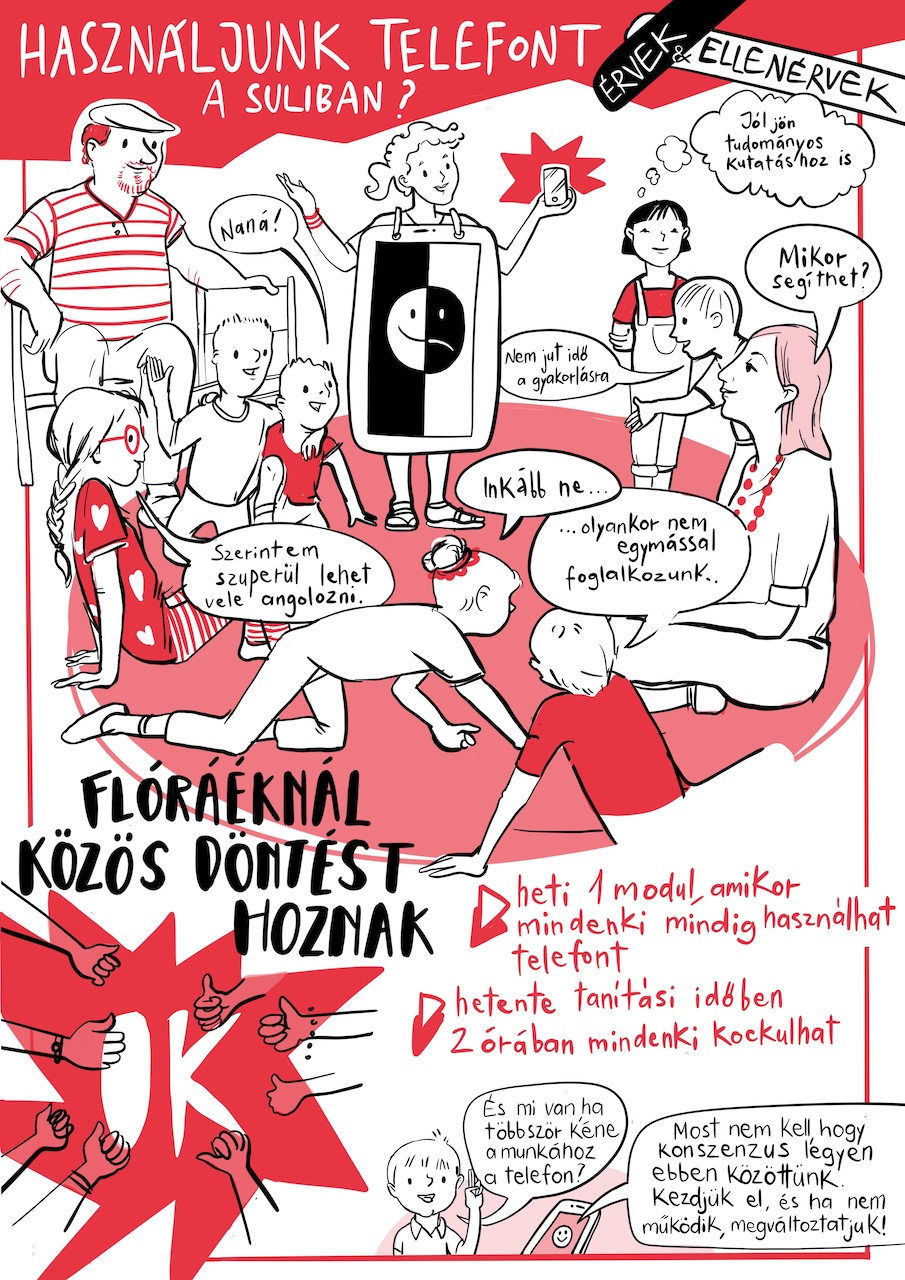
\includegraphics{pics/5b_dontes.jpg}
\caption{A szabályok célja, hogy a közösséget szolgálja.}
\end{figure}

\hypertarget{konfliktusok-feszultsegek-kezelese}{%
\subsection{Konfliktusok, feszültségek
kezelése}\label{konfliktusok-feszultsegek-kezelese}}

Tudjuk, hogy a Budapest School szereplői, a gyerekek, a tanárok, a
szülők, a pedagógiai program, a kerettanterv, a fenntartó, a szomszédok,
az állami hivatalok között feszültségek és konfliktusok alakulhatnak ki,
mert különbözőek vagyunk, különbözőek az igényeink. A feszültségekre és
a konfliktusokra a Budapest School olyan lehetőségként tekint, amelynek
együttműködésen alapuló megoldása építi a kapcsolatot, és segíti a
fejlődést.

Minden vágy, ötlet, szándék, cél, viselkedés közötti különbség, ha az
valamelyik félben negatív érzéseket kelt, feszültséget és konfliktust
okozhat. Ebbe beletartozik az is, ha valaki nem azt és úgy csinálja,
ahogy nekünk erre szükségünk van, vagy ha bármilyen okból nem érezzük
magunkat biztonságban, vagy más univerzális emberi szükségletünk
{\autocite{Rosenberg2003}} nem elégül ki.

Konfliktus alakulhat ki a gyerekek, szülők és tanárok között bármilyen
relációban, és adódhatnak egyéb, belső konfliktusok, nehézségek is akár
a család, akár a Budapest School életében, amelyek kihathatnak a
közösségi kapcsolatainkra.

\begin{figure}
\centering
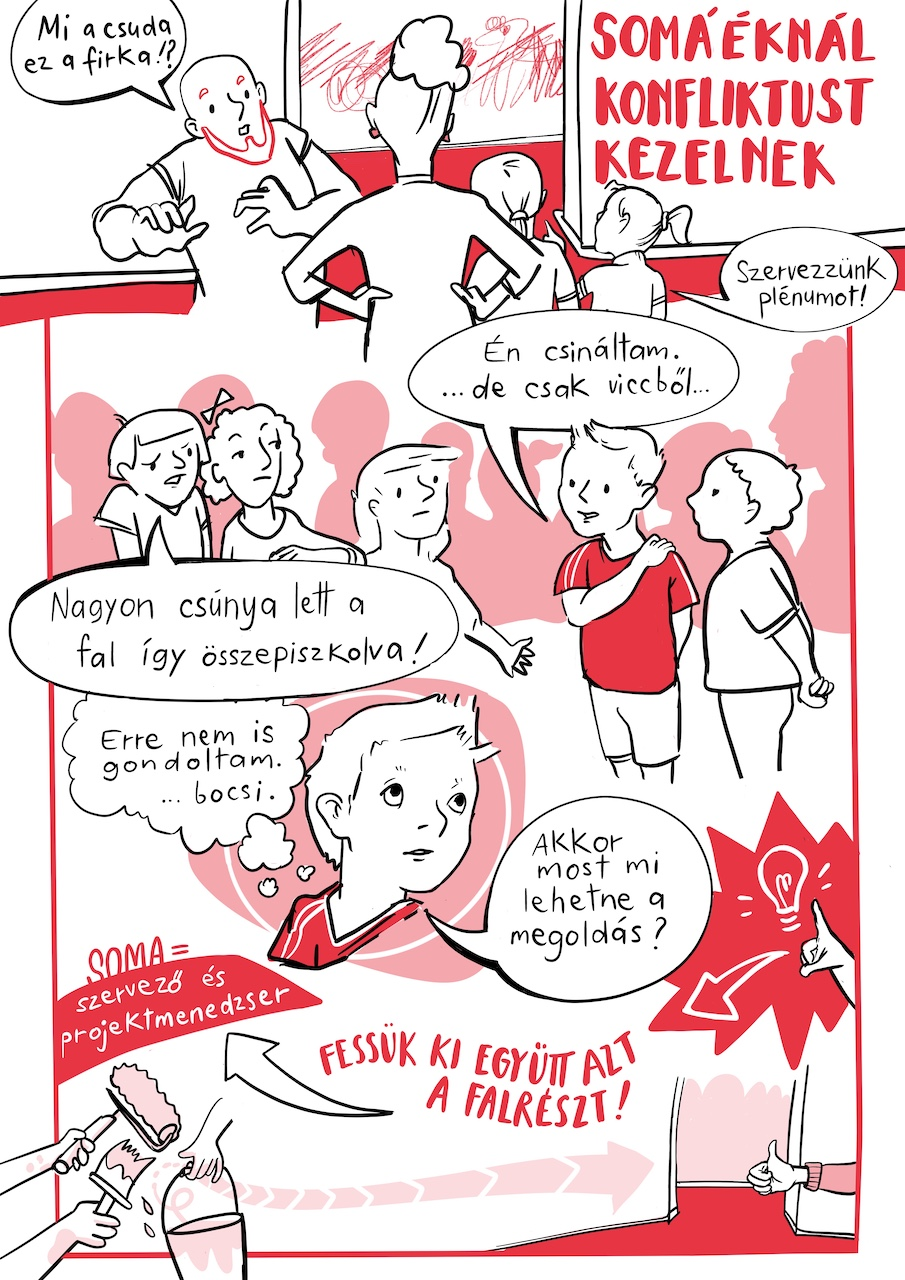
\includegraphics{pics/5a_konfliktus.jpg}
\caption{Konfliktus esetén a felborult egyensúly helyreállítására törekszünk.}
\end{figure}

\hypertarget{a-bps-konfliktusok-feloldasa}{%
\subsubsection{A konfliktusok feloldása a BPS-ben}\label{a-bps-konfliktusok-feloldasa}}

Az iskola partnerségen alapuló szervezetében nem autoritások, főnökök,
hivatalok, bírók oldják meg a konfliktusokat, hanem egyenrangú társak.
Az iskola feltételezi, hogy a felek tudnak gondolkodni, következtetni,
felelősséget vállalni a döntéseikért és cselekedeteikért. A kisgyerekeket
mentoraik és szüleik képviselik.

\hypertarget{alapertekek}{%
\paragraph{Alapértékek}\label{alapertekek}}

Ahhoz, hogy tényleg partneri kapcsolatban, egyenrangú\break
felekként lehessen
konfliktusokat, problémákat megoldani, érdemes közös értékeket
elfogadni.

\begin{itemize}
\tightlist
\item
  Először a saját változásunkon dolgozunk, mert másokat nem nagyon tudunk
  megváltoztatni, csak a magunk változásáért lehetünk felelősek.
\item
  Felelősséget vállalunk gondolatainkért, hiedelmeinkért, szavainkért
  és viselkedésünkért.
\item
  Nem pletykálunk, szóbeszédet nem terjesztünk.
\item
  Nem beszélünk ki embereket a hátuk mögött.
\item
  A félreértéseket tisztázzuk, a konfliktusokat felszínre hozzuk.
\item
  A problémákat személyesen, szemtől szembe beszéljük meg, másokat nem
  húzunk bele a problémába.
\item
  Nem hibáztatunk másokat a problémákért. Amikor mégis, akkor az
  jó alkalom arról gondolkozni, hogy miként vagyunk mi is része a
  problémának, és miként kell a megoldás részévé válnunk.
\item
  Az erősségekre több figyelmet fordítunk, mint a gyengeségekre, és a
  lehetőségekről, a megoldásokról többet beszélünk, mint a problémákról.
\end{itemize}

\hypertarget{feszultseg-felszinre-hozasa}{%
\paragraph{A feszültségek felszínre
hozása}\label{feszultseg-felszinre-hozasa}}

Olyan módszereket, folyamatokat, szabályokat, szokásokat kell
kialakítani minden közösségben, hogy legyen tere és ideje a
feszültségeket előhozni.

\begin{itemize}
\tightlist
\item
  Az iskolai csoportok rendszeresen egy bejelentkező
  körrel kezdik a napjukat, ahol van lehetőség a problémákat is
  megbeszélni.
\item
  A csoportok rendszeresen tartanak retrospektív gyűlést, ahol értékelik, mi volt jó, és mi nem volt annyira jó egy vizsgált időszakban.
\item
  Évente legalább kétszer a tanárok egymásnak, a szülők a tanároknak, a gyerekek a tanároknak, a tanárok a gyerekeknek szervezett formában
  visszajelzést adnak.
\item
  A gyerekek a mentorukkal rendszeresen találkoznak, és ilyenkor teret kapnak a felmerülő feszültségek.
\end{itemize}

\hypertarget{megbeszeles}{%
\paragraph{Megbeszélés}\label{megbeszeles}}

A Budapest School közösségének valamennyi tagja (a tanárok, gyerekek,
szülők, adminisztrátorok, iskolát képviselő fenntartó)\break
vállalja:

\begin{itemize}
\tightlist
\item
  A közösség mindennapjaival kapcsolatos konfliktusok esetén elsőként az
  abban érintett személynek jelez közvetlenül.
\item
  A személyes kritikát mindig privát csatornán fogalmazza meg először,
  ha kell, akkor segítő bevonásával.
\item
  Bármelyik fél jelzése esetén lehetőséget biztosít arra, hogy a vitás
  kérdést közvetlenül megbeszéljék, a folyamatban részt vesz.
\item
  Szakítás, kilépés, lezárás előtt legalább három alkalommal megpróbál
  egyeztetni.
\item
  Az egyeztetésre elegendő időt hagy, amely legalább 30 nap,
 vagy\break
 (ha ennél több időre van szükség) a másik féllel megállapodott
  idő.
\item
  Teljes figyelemmel, nyitottsággal, a probléma megoldására fó\-ku\-szál\-va
  igyekszik feloldani a konfliktust, és közösen megoldást találni a
  problémára.
\end{itemize}

Összefoglalva: ha problémánk van egymással, akkor azt megbeszéljük. Nem
okozunk egymásnak meglepetést, mert vállaljuk, hogy rögtön elmondjuk
egymásnak gondjainkat.

\hypertarget{kozvetito-bevonasa}{%
\paragraph{Közvetítő bevonása}\label{kozvetito-bevonasa}}

Ha úgy érezzük, hogy a személyes egyeztetés nem vezetett megoldásra, a
tárgyalást külső segítség bevonásával folytatjuk. Ez lehet egy másik
csoporttag, egy tanár, vagy egy teljesen külsős mediátor.

Amikor bármely fél közvetítőt kér, akkor a másik ezt elfogadja. Nem
mondhatjuk azt, hogy ~\emph{„de hát mi magunk is meg tudjuk oldani a
konfliktust''}.

\hypertarget{eszkalalas}{%
\paragraph{Eszkalálódás}\label{eszkalalas}}

Ha két fél nem tudja megoldani a konfliktust, akkor kérhetnek segítséget
a \texttt{segitseg@budapestschool.org} címen, amire 48 órán belül kell
választ kell kapniuk. Az e-mail kezeléséért az iskola fenntartója felel.

\hypertarget{megallapodasok}{%
\paragraph{Megállapodások}\label{megallapodasok}}

Ha az egyeztetés, tárgyalás és közvetítő bevonása során sikerül
valamilyen megoldást vagy a megoldáshoz vezető folyamatot egyeztetni, a
felek \emph{megállapodnak} abban, hogy ki mit tesz, vagy milyen
szabályokat alakítanak ki, illetve hogy mennyi időt adnak egymásnak,
hogy kipróbálják, sikerült-e feloldani a konfliktust. Segíteni szokott a
kérdés, hogy \emph{most megállapodtunk vagy csak beszéltünk róla?}

Nagyobb konfliktusok esetén jó gyakorlat, és ezt bármely fél kérheti, hogy
írásban is rögzítik a megállapodást. Ez lehet egy papírfecni is vagy
egy e-mail. Lényege nem a formátum, hanem hogy minden fél emlékezzen a
megállapodásra.

\hypertarget{ha-az-egyeztetes-sikertelen}{%
\paragraph{Ha az egyeztetés
sikertelen}\label{ha-az-egyeztetes-sikertelen}}

Ha a felek között az egyeztetés sikertelen volt, vagy a megoldási
javaslat nem működött, a feleknek ezt írásban meg kell állapítaniuk.
Erre azért van szükség, hogy egyetértés legyen közöttük abban, hogy
értik, a másik fél sikertelennek érzi az egyeztetést.

\hypertarget{lezaras}{%
\paragraph{Lezárás}\label{lezaras}}

Az egyeztetés sikertelensége esetén elengedjük egymást. De ez a végső
megoldás.

\hypertarget{kiemelt-konfliktusok}{%
\subsection{Kiemelt konfliktusok}\label{kiemelt-konfliktusok}}

\hypertarget{gyerek-gyerek-konfliktus}{%
\subsubsection{Gyerek---gyerek
konfliktus}\label{gyerek-gyerek-konfliktus}}

A mindennapokban a gyerekek akarva-akaratlanul is belecsöppennek\break
olyan
helyzetekbe, amikor a közösségben vagy interperszonális kapcsolataik
során megborul a mindennapi egyensúly. Ezekben a konfliktushelyzetekben
leginkább a felborult egyensúly helyreállítására törekszünk
\emph{helyreállító konfliktusfeloldási technikával}.

A helyreállító konfliktusfeloldás alaptézise az, hogy minden ilyen
megborult egyensúlyi állapot egy lehetőség valaminek a megújítására,
újragondolására. A résztvevők egy külső személy segítségével (általában
a jelen lévő tanáréval) alakítják a megoldást, egészen addig, amíg az
eredmény mindenki számára a konfliktus feloldását, azaz a
megborult egyensúly helyreállítását jelenti.

A folyamat során a konfliktusban részt vevő összes személy elmondja az
érzéseit, meglátását a felmerülő helyzettel kapcsolatban, valamint az
én-közléseken túl a szükségleteikről is beszélnek. Ezen szükségletek
képezik a megoldás alapját, azaz ezeket egy tető alá hozva feloldhatjuk
a fennálló konfliktust. Ilyenkor mindig először azokat a pontokat
keressük meg, amelyekben egyetértenek a résztvevők, hiszen ez közös
alapot szolgáltat arra, hogy a valódi feloldást megtalálhassuk.

Fontos, hogy a beszélgetésben az összes fél hallassa a hangját, és meg
is legyen hallgatva. Az értő figyelem kompetenciája is fejlődik ezen
módszer alkalmazása során, például, ha az érintett felek elmondják, hogy
mit hallottak meg abból, amit a másik elmondott.

Előfordulhat, hogy ez a folyamat nem egyből a konfliktus után indul el:
ha a résztvevők beleegyeznek, akkor a beszélgetés elhalasztható, de
lehetőleg még aznap történjen meg.

\hypertarget{gyerek-iskola-tanar-szulo-konfliktus}{%
\subsubsection{Gyerek---iskola és tanár---szülő
konfliktus}\label{gyerek-iskola-tanar-szulo-konfliktus}}

Minden gyereknek van egy mentora. A szülők számára a mentor az
elsődleges kapocs az iskolával. Ezért, ha a szülőben jelenik meg egy
feszültség, akkor elsődlegesen a mentornak jelez. Ugyanígy a mentor
közvetíti a család felé a gyerekkel kapcsolatos feszültségeket.

Ha egy gyerek vagy szülő úgy érzi, hogy egy gyereknek nem jó az iskolai
élménye, például nem tanul eleget, vagy kiközösítik, vagy csak nem
szeret bemenni, akkor feladata, hogy rögtön beszéljen a mentorral.

Ha nem sikerül a mentorral megbeszélni a konfliktust és megoldást
találni, akkor a szülőnek is lehetősége van segítőt behívni, aki lehet
egy másik tanár, másik szülő, az iskolaigazgató vagy bárki, akinek
képességeiben bízik.

Előfordulhat, hogy a tanárok vagy az iskola úgy érzik, hogy egy
gyereknek nem tesz jót a Budapest School közössége, vagy a hozzáállása
súlyosan zavarja vagy sérti a Budapest School közösséget vagy azok
tagjait. Az is lehet, hogy a tanárok vagy a Budapest School a szülővel
való kapcsolatot érzik konfliktus vagy feszültség forrásának. Ilyen
esetben ugyanígy le kell folytatni a konfliktuskezelés folyamatát, és
meg kell próbálni feloldani a feszültséget. Ennek sikertelensége esetén az
iskola írásban jelzi a családnak, hogy el fognak válni.

\hypertarget{bps-modell-egyedi-program-hazirend-be-nem-tartasaval-kapcsolatos-konfliktusok}{%
\subsubsection{BPS modell, egyedi program, házirend be nem tartásával
kapcsolatos
konfliktusok}\label{bps-modell-egyedi-program-hazirend-be-nem-tartasaval-kapcsolatos-konfliktusok}}

Amikor egy tanár, egy gyerek vagy egy tanulóközösség nem tartja be az
egyedi programot, a házirendet, vagy egyéb közösen megalkotott
szabályokat, akkor konfliktus alakul ki közte és az iskola között.
Ilyenkor szintén a konfliktuskezelés folyamatát kell alkalmazni.

\hypertarget{minosegfejlesztes-folyamatszabalyozas}{%
\section{Minőségfejlesztés,
folyamatszabályozás}\label{minosegfejlesztes-folyamatszabalyozas}}

Honnan tudjuk, hogy jól működik az iskola? Minden gyerek azt tanulja,
amit szeretne, és amire neki a leginkább szüksége van? Megkérdezzük az
érintetteket, figyeljük az adatokat, és azok alapján fejlesztünk.

A Budapest School-iskolában a gyerekek tanulását egy komplex rendszer
egyik elemének tekintjük {\autocite{Barabasi2007}}. Iskoláink a
világ felé nyitott hálózatot alkotnak: az egy közösségben lévő gyerekek,
a családok, a velük foglalkozó tanárok, a helyi környezet, a Budapest
School további közösségei, az ország és a nemzet állapota, valamint a
globális társadalmi folyamatok is befolyásolják, hogy mi történik egy
iskolában.

Hogy egy gyerek épp mit és mennyit tanul, az nemcsak az iskola programjától
vagy a NAT-tól, hanem számos más tényezőtől is függ, melyek
befolyásolják a fejlődést és a közösség egymás fejlődésére gyakorolt
hatását: többek közt függ a gyerekek múltjától, aktuális hangulatától és
vágyaitól, a tanárok személyiségétől, a családtól, a csoportdinamikától
és a társadalomban történő változásoktól is.

Ezért a gyermekeink fejlődését, tanulását és boldogságának alakulását
egy \emph{komplex rendszer} működésével modellezhetjük.
\newpage
A tanulási folyamataink minőségfejlesztésénél a következő szempontokat
vesszük figyelembe:

\begin{enumerate}
\def\labelenumi{\arabic{enumi}.}
\tightlist
\item
  A történéseket, eseményeket, (rész)eredményeket folyamatosan kell
  monitorozni.
\item
  A visszajelzéseket a rendszer minden tagjától folyamatosan gyűjteni
  kell: a gyerekektől, tanároktól, szülőktől és az adminisztrátoroktól.
\item
  Anomália esetén a helyzetfelismerés, az eltérések okának felkutatása a
  cél.
\item
  A feltárt hibák alapján a rendszert folyamatosan kell javítani.
\end{enumerate}

A minőségfejlesztés célja az iskola mint tanulórendszer folyamatos
fejlesztése. A monitorozás folyamatos, így az iskola hamar felismeri az
anomáliákat, és kivizsgálás után, ha szükséges, meg tudja azokat
szüntetni, tanulni is tud belőlük, és javítja a rendszert.

A fenntartó folyamatosan monitorozza a tanulóközösségeket és
visszajelzéseket ad, aminek alapján a tanulóközösség javítja a saját
működési folyamatait. A BPS modellben leírt működést a fenntartó mérhető
és megfigyelhető indikátorokra fordítja le, és kidolgozza, üzemelteti a
metrikák 2-3 hónapnyi rendszerességű nyomon követésére alkalmas
rendszerét.

A fenntartónak meg kell figyelnie legalább a következő metrikákat:

\begin{enumerate}
\def\labelenumi{\arabic{enumi}.}
\tightlist
\item
  A szülő, a gyerek és a tanár közötti saját célokat megfogalmazó hármas
  megállapodások időben megszülettek, nincs olyan gyerek, akinek nincs
  elfogadott saját tanulási célja. Indikátor: elkészült szerződések
  száma.
\item
  A modulok végén a portfóliók bővülnek, és azok tartalma a
  tantárgyakhoz kapcsolódik. Indikátor: a portfólió elemeinek száma és
  kapcsolhatósága.
\item
  A
  tanulási eredményekre (\ref{tantargyak}.~fejezet, \pageref{tantargyak}.~oldal)
  vonatkozó megkötések időben teljesülnek. Indikátor: elért tanulási
  eredmények száma gyerekekre bontva.
\item
  A szülők biztonságban érzik gyereküket, és eleget tudnak
  arról,\break
  hogy
  mit tanulnak. Indikátor: kérdőíves vizsgálat alapján.
\item
  A tanárok hatékonynak tartják a munkájukat. Indikátor: kérdőíves
  felmérés alapján.
\item
  A gyerekek úgy érzik, folyamatosan tanulnak, támogatva vannak, vannak
  kihívásaik. Indikátor: kérdőíves felmérés alapján.
\end{enumerate}

\hypertarget{tanarok-kivalasztasa-tanulasa-fejlodese-es-ertekelese}{%
\section{Tanárok kiválasztása, tanulása, fejlődése\break
és értékelése}\label{tanarok-kivalasztasa-tanulasa-fejlodese-es-ertekelese}}

Az iskola legmeghatározóbb összetevői a tanárok. Ezért a Budapest School
külön figyelmet fordít arra, hogy ki lehet tanár az iskolákban, és
hogyan segítjük az ő fejlődésüket.

\paragraph{Alapelveink}
        
\begin{enumerate}
\def\labelenumi{\arabic{enumi}.}
\tightlist
\item
  Minden tanárnak tanulnia kell. Amit ma tudunk, az nem biztos, hogy
  elég arra, hogy a holnap iskoláját működtessük. És az is biztos, hogy
  még sokkal hatékonyabban lehetne segíteni a gyerekek tanulását, mint
  amilyenek a ma ismert módszereink.
\item
  A tanároknak csapatban kell dolgozniuk, mert összetett
  (interdiszciplináris) tanulást csak vegyes összetételű (diverz)
  csapatok tudnak támogatni.
\item
  A szakképesítés nem szükséges és nem elégséges feltétele annak, hogy a
  Budapest Schoolban valaki jól teljesítő tanár legyen.
\end{enumerate}

\hypertarget{felvetel}{%
\paragraph{Felvétel}\label{felvetel}}

A Budapest School tanulásszervező tanárainak felvétele egy legalább
háromlépcsős folyamat, ahol vizsgálni kell a tanár egyéniségét
(attitűdjét), felnőtt---felnőtt kapcsolatokban a viselkedésmódját (társas
kompetenciáit), és minden jelöltnek próbafoglalkozást kell tartania,
amit az erre kijelölt Budapest School-tanárok megfigyelnek. A felvételi
folyamatot a fenntartó felügyeli és irányítja.

\hypertarget{sajat-cel}{%
\paragraph{Saját cél}\label{sajat-cel}}

Minden tanárnak van saját, egyéni fejlődési célja: \emph{mitől tudok én
jobb tanár lenni, jobban támogatni a gyerekek tanulását, segíteni a
munkatársaimat és partnerként dolgozni a szülőkkel?}

\hypertarget{tanarok-mentora}{%
\paragraph{Tanárok mentora}\label{tanarok-mentora}}

A gyerekekhez hasonlóan minden tanárnak van mentora, aki segíti a
saját céljainak kialakításában, és folyamatosan támogatja ezek elérésében.

\hypertarget{tanarok-ertekelese}{%
\paragraph{Tanárok értékelése}\label{tanarok-ertekelese}}

Minden tanárt évente legalább kétszer értékelnek a munkatársai. Ez az a
folyamat, amit 360 fokos értékelésnek hívnak az üzleti szférában. A
visszajelzések feldolgozása után a saját célokat frissíteni kell.

Minden tanárt értékelnek a szülők is (kifejezetten a mentorált gyerekek
szülei) és a gyerekek is legalább évente kétszer.

\hypertarget{a-felvetel-es-az-atvetel}{%
\section{A felvétel és az átvétel}\label{a-felvetel-es-az-atvetel}}

Aki a BPS iskolához csatlakozik, az rögtön a BPS egyik
tanulóközösségéhez csatlakozik. A tanulóközösségéhez bármikor lehet
csatlakozni, ha és amikor a csatlakozó család ezt szeretné, és ha ettől
a tanulóközösség minden tagjának valamiért jobb lesz, vagy nem változik
(de rosszabb nem lehet). Az iskola nem azért fogad be valakit, mert 
kénytelen, hanem mert a tanulóközösség ezt szeretné. A családok nem azért
csatlakoznak, mert valamit kell találni a gyereknek, hanem mert
szeretnének a Budapest School egyik tanulóközösségéhez tartozni.

A 12 évfolyamos egységes iskolába bármikor lehet csatlakozni, az iskola
normálisnak tartja, hogy a közösség tagjai változnak. Ezért az iskolában
egy iskolát most kezdő 6 éves felvétele, egy 8 éves, az előző iskoláját
nem kedvelő felvételi kérelme, egy 9 éves külföldről hazaköltöző év
közbeni csatlakozása, egy 12 éves „gimnáziumba'' jelentkezése és egy 16
éves más városból érkező között az iskola számára a \emph{felvételi és
átvételi folyamatot} tekintve nincs különbség.

Ahhoz, hogy egy család csatlakozzon a tanulóközösséghez, kizárólag egy tanulóközösség tanulásszervezőinek a hozzájárulása
szükséges.

Egy család jelentkezése után legalább három dolognak kell történnie.

\begin{itemize}
\item
  A családnak meg kell ismernie a Budapest School alapelveit, működését, jellegzetességeit. Az iskolának meg kell mutatnia önmagát. A családnak meg kell értenie, és meg kell fogalmaznia, hogy miért akarnak csatlakozni a közösséghez.
\item
  A tanulásszervezőknek meg kell ismerniük a családot, megnézni, hogy „működik-e a kémia'', tudják-e vállalni a gyerek tanulásának támogatását.
\item
  A gyereknek időt kell eltöltenie a tanulóközösségben, a mindennapokhoz minél inkább hasonló körülmények között, hogy mindenki meg tudja tapasztalni, érezni, hogy milyen lenne együtt és egymástól tanulni.
\end{itemize}

\hypertarget{szempontok-a-donteshez}{%
\subsection{Szempontok a döntéshez}\label{szempontok-a-donteshez}}

A tanulóközösség legyen minél inkább diverz és kiegyensúlyozott: kevert
korosztályú, kevert nemi, kevert szociális státuszú, kevert érdeklődésű,
kevert személyiségjegyű csoport, úgy, hogy legyen egy erős, mindenkit
megtartó szociális háló. A tanulóközösségek közösségét egyenként kell
kiegyensúlyozni.

Így az is előfordulhat, hogy egy gyerek egy tanulóközösségben nem talál
helyet magának, de az iskola egy másik tanulóközösségében igen. Mert a
közösségek különbözőek. A legegyszerűbb példa: van, ahol több lányt
szeretnénk, mint ma, és van, ahol több fiút, és van, ahol ez most nem
szempont.

\hypertarget{nincs-felveteli-vizsga}{%
\subsection{Nincs felvételi vizsga}\label{nincs-felveteli-vizsga}}

Az iskola nem követel meg sem írásbeli (központi), sem szóbeli felvételit,
és nem is az előző iskolák osztályzatai alapján dönt. Az egyetlen
szempont az,
hogy jobban tud-e működni egy tanulóközösség egy gyerek (és család)
csatlakozásával. A döntést a tanulóközösség tanárai, a fenntartó (vagy
delegáltja) és a család hozzák meg.

\hypertarget{szakitas-tavozas-elengedes}{%
\subsection{Szakítás, távozás,
elengedés}\label{szakitas-tavozas-elengedes}}

Működésünk része, hogy konfliktusok, kényelmetlenségek, változó
körülmények között, aki egyszer csatlakozott, az egyszer távozhat is a
közösségből.

\begin{itemize}
\item
  Az iskola, a tanárok és a család alapelvei, értékei közötti különbségek okozhatnak annyi és olyan konfliktust, amit már nem tudnak a felek feloldani.
\item
  Van, hogy egy gyerek nem találja meg a helyét, vagy épp valamiért elkezd a közösségben „nem boldog'' pozícióba kerülni. Vagy épp a közösség többi tagjának lesz kényelmetlen az együttlét.
\item
  A családok élete, vágyai, motivációjuk, körülményei változhatnak úgy, hogy épp más közösségben jobb helyet találnának.
\end{itemize}

Bármi legyen is az ok, a távozás, szakítás feszültséggel teli szituáció.
Ezért is fontos, hogy minden fél betartsa a közösségi lét szabályairól
szóló fejezetben (\ref{a-kozossegi-let-szabalyai}.~fejezet, \pageref{a-kozossegi-let-szabalyai}.~oldal) leírt
konfliktuskezelési szokásokat
(\pageref{konfliktusok-feszultsegek-kezelese}. oldal).

A csatlakozáskor a családok szerződésben vállalják a jelen program és az
iskola egyéb szabályozóinak betartását --- ennek ismételt vagy súlyos
megszegése esetén az iskola jogosult a tanulói jogviszonyt megszüntetni.
Ez a döntés a fenntartó jogkörébe tartozik.

\hypertarget{hianyzasok-mulasztasok-igazolasok-kesesek}{%
\section{Hiányzások, mulasztások, igazolások,
késések}\label{hianyzasok-mulasztasok-igazolasok-kesesek}}

A Budapest School feladata, hogy olyan környezetet biztosítson a
gyerekeknek, amiben boldogak, felszabadultak, magabiztosak és hatékonyak
tudnak lenni. Budapest School családok maguk és önszántukból választják
ezt az iskolát, áldoznak sok időt és energiát arra, hogy az iskolában
tudjanak tanulni. \emph{Ezért az iskola feltételezi, hogy a gyerekek az
iskolában akarnak tanulni önszántukból}.

Sok oka lehet annak, hogy egy gyerek még sincs az iskolában. Például

\begin{itemize}
\item
  betegnek, fáradtnak érezheti magát, fizikailag vagy lelkileg kimerült,
  vagy lehet valamilyen fertőző betegsége;
\item
  családjával tölt értékes, minőségi időt, mert fejlődését ez szolgálja
  a leginkább;
\item
  előre nem tervezett esemény miatt nem tud az iskolába menni;
\item
  utazik, felfedez, külső helyszínre szervezett tanulási programokon
  vesz részt;
\item
  egy projektjébe úgy belemerül, hogy érdemesnek találja nem az
  iskolában, fókuszáltan végezni a munkát.
\end{itemize}

A fenti példák is két jól elkülöníthető kategóriába sorolhatóak. A
\emph{nem tervezett hiányzástól} jól elkülöníthetőek azok az esetek,
amikor a gyerek, bár nem az iskolában tartozkodik, mégis szervezett,
strukturált módon biztosított a fejlődése, tanulása. Ezt az esetet a
\emph{„távmunka``\emph{ mintájára }„távtanulásnak''} hívja az iskola,
mert ezt az időt is tanulásra szánjuk.

Alapelv, hogy \emph{a mentornak, gyereknek és szülőnek meg kell
állapodni a távtanulásról}. Minden félnek tudnia kell róla, meg kell
előre tervezni és nem lehet esetleges. Mindenképpen meg kell
különböztetni a \emph{nem tervezett hiányzástól}.

\hypertarget{tervezett-tavtanulas}{%
\paragraph{Tervezett távtanulás}\label{tervezett-tavtanulas}}

Előre eltervezett módon, valamilyen program miatt nincs a gyerek az
iskolában. Ilyenkor a mentor és a gyerek megtervezi a tanulás célját,
várható eredményeit. A terv létrejöttéért a gyerek és a szülő felelős,
és minden félnek el kell fogadnia a tervet. Tehát a mentornak hozzá kell
járulnia. Ha a mentor nem járul hozzá, akkor addig nem kezdhető meg a
távtanulás, amig megállapodás nem születik. Ha mégis, akkor azt nem
tervezett hiányzásnak kell tekinteni.

Ha a tervezett távtanulás elérte a 20 napot vagy 160 órát, akkor a
mentor mellett egy másik mentor szerepben dolgozó tanulásszervezőnek is
meg kell ismernie és el kell fogadnia a tervet. 40 nap felett három
mentornak kell együtt elfogadnia a tervet, melyek egyike egy másik
tanulóközösség mentora.

\hypertarget{nem-tervezett-hianyzas}{%
\paragraph{Nem tervezett hiányzás}\label{nem-tervezett-hianyzas}}

A gyerek és a mentortanár nem tud előre felkészülni az iskolán kívüli
tanulásra, mert a hiányzás előző nap vagy aznap derül ki, vagy más okból
a megállapodás nem jön létre. A szülő feladata, hogy még ebben az
esetben is erről reggel 9 óra előtt értesítse a mentortanárt.
Mikroiskolánként eltérhet a preferált kommunikációs eszköz, ezért a
tanulásszervezők feladata meghatározni, hogyan kérik az értesítés
formáját.

Egy tanévben 15 munkanap, vagy 120 óra, de alkalmanként csak 5 munkanap,
nem megtervezett hiányzást igazolhat a szülő (rögzített és dokumentált
módon). Orvos által igazolt betegség, hatósági intézkedés és egyéb
alapos indok esetén a 20/2012. (VIII.~31.) EMMI-rendelet 51.~§~(2)
értelmében igazoltnak kell tekinteni a hiányzást.

\hypertarget{igazolatlan-hianyzas}{%
\paragraph{Igazolatlan hiányzás}\label{igazolatlan-hianyzas}}

Az az eset, amikor a szülő vagy a mentortanár nem tudott a hiányzásról,
nem volt előre megtervezve, vagy a 15 napos, 120 órás keret kimerült.
Ebben az esetben az iskola szigorúbban jár el, mint általában más
iskolák. Ilyenkor a 20/2012. (VIII.~31.) EMMI-rendelet 51.~§~(3) pontja
értelmében minden esetben az iskola értesíti a szülőt, és 10 igazolatlan
óra után figyelmezteti, hogy a következő igazolatlan után \emph{„az
iskola a gyermekjóléti szolgálat közreműködését igénybe véve megkeresi a
tanuló szülőjét"}. Az iskola megközelítése egyszerű: mivel partneri
viszonyban van a tanár, gyerek és szülő, ezért az alapértelmezett az,
hogy vagy előre meg lehetett volna beszélni a hiányzásokat, amely
esetben tervezett távtanulásról beszélnénk, vagy betegség miatt kellett
túllépni a 15 napot. Elég tág keretet enged az iskola. Abban az esetben
azonban, amikor a gyerek vagy a szülő nem tartja be a kereteket, nem él
a partneri viszonnyal, akkor ott valami baj van. Gyorsan kell reagálni.

\hypertarget{hogyan-biztositja-a-rendszer-a-visszaelesek-kikuszoboleset}{%
\subsubsection{Hogyan biztosítja a rendszer a visszaélések
kiküszöbölését}\label{hogyan-biztositja-a-rendszer-a-visszaelesek-kikuszoboleset}}

A Budapest Schoolba járó gyerek szülei és tanárai egyetlen igazolatlan
óra hiányzás után értesítést kapnak arról, hogy a gyerek nem jelent meg
az iskolában. Tehát egy gyerek nem tud szülei tudta nélkül távolmaradni.

Egy szülő 15 napon keresztül „igazolhat" nem tervezett hiányzást, hogy
ne kelljen minden náthánál a körzeti orvosi rendszert terhelni, ahogy
azt a Házi Gyermekorvosok Egyesülete javasolja. Miért feltételezzük,
hogy nem él ezzel vissza a szülő és a gyerek? Mert az iskolában maradás
feltétele a tanulás és a folyamatosan újra felállított tanulási célok
követése. Az ezzel való visszaélés az iskola céljaival ellentétes és
legkésőbb a soron következő trimeszter tanulási szerződésekor a
felszínre kerül.

A távtanulást pedig nem tekinti az iskola hiányzásnak, mert a tanulás
folytatólagos, dokumentált, megtervezett. A portfóliók bővülését pedig
folyamatosan monitorozza az iskola. A mentortanár és a gyerek tévesen
mérheti fel a helyzetet, és előfordulhat, hogy tanulásnak, fejlődésnek
látnak valamit, ami nem az. Ezért került a rendszerbe a „külső
megfigyelő" kitétel, hogy 20 nap után új tanárt kell bevonni a döntésbe.
Ha a gyerek tanulási veszélybe kerül, akkor az a tanulási eredmények
elmaradásából fél éven belül felfedezhető.

\hypertarget{kesesek-kezelese}{%
\subsection{Késések kezelése}\label{kesesek-kezelese}}

A Budapest School tanulóközösségek maguk állítják fel a napirenddel
kapcsolatos kereteket: mikor kezdenek, meddig tartanak a strukturált
foglalkozások, mikor vannak a szünetek, és hogyan kezdődik újra a nap
folyamán a fókuszált munka. A kereteket a tanulásszervező tanárok
feladata kialakítani és trimeszterenként megkezdése előtt kihirdetni.

Fontos, megbeszélendő részlet, hogy hogyan kezeli a közösség a
késéseket: mikortól lehet érkezni, mikor kezd a közösség annyira
dolgozni, hogy zavaró, amikor valaki belép és megzavarja a folyamatot.
Megállapodást köt a közösség, hogy hogyan kívánja kezelni a késéseket,
mi segíti a csapatot leginkább a céljai elérésében.

Az iskola nem regisztrálja a késéseket, mert az iskola nem tudhatja,
hogy egy-egy késés elfogadható-e a közösségnek vagy nem. Egy színdarab
főpróbájáról 5 percet késni mást jelent a közösség számára, mint arról
az óráról, ahol mindenki egyedül füllhallgatóval böngészi egy online
tananyag számára legrelevánsabb fejezetét.

Ha egy csoportot megzavar valakinek az ismételt késése, akkor konfliktus
alakul ki a csoport és a késő vagy a tanár és a késő között. Ezt a
típusú konfliktust (is) .~fejezet szerint kell feloldani.

\hypertarget{ki-viheti-el-a-gyereket}{%
\section{Ki viheti el a gyereket?}\label{ki-viheti-el-a-gyereket}}

Gyereket bárki behozhat az iskolába, de elvinni csak az viheti el, akit
a gyerek szülei ---~a fenntartó által üzemeltetett számítógépes
rendszeren keresztül~--- felhatalmaztak. Gyerek egyedül csak akkor mehet
el az iskolából, ha erre a szülei engedélyt adtak. Ezek a
felhatalmazások lehetnek egyszeriek, határidőhöz kötöttek vagy
visszavonásig érvényesek.

\hypertarget{sarga-narancs-piros-riasztas}{%
\section{Sárga, narancs, piros
riasztás}\label{sarga-narancs-piros-riasztas}}

A BPS-tanulóközösségek bonyolult rendszerként működnek. A tanulóközösség
tagjai, a gyerekek, a tanárok, a szülők és a környezet kölcsönhatásban vannak
egymással: az egyikünk tettei kihatnak a többiekre. Az, hogy egy gyerek
hogyan viselkedik a csoportban, úgyanúgy függ a személyiségétől,
a képességeitől és a csoport, a többi gyerek és a tanárok működésétől is.
Vannak, olyan nehézségek, konfliktusok, feszültségek, amikor úgy érzi
valamelyik csapattag, hogy tenni kell valamit, mert a helyzet sokáig nem
tartható. Ilyenkor \emph{riasztást} küld az érintetetteknek.

Mikre is gondolunk?

\begin{itemize}
\tightlist
\item
  Abony zavarja a többieket a foglalkozáson, mert eltereli a figyelmet.
\item
  Fáni állandóan cukkolja, zaklatja a társait. Bántó, sértő
  megjegyzéseket tesz.
\item
  Orku kirántja társa kezéből az ollót, nem kéri el, és nem tud várni.
\item
  Barka nem képes a többiekkel haladni a matekórán. Nem zavar senkit, és
  nagyon édes, amikor bámul kifelé az ablakon. Látjuk rajta, hogy egyre
  szomorúbb a szeme, és már olyanokat mond, hogy ,,én nem vagyok jó
  matekból''.
\item
  Kinga jól érzi magát a BPS-ben, de szülei régóta elégedtelenek, és néha
  kiabálnak a tanárokkal, agresszív e-maileket küldenek.
\end{itemize}

A példák jól mutatják, hogy a nehézségeknek mindig több oka van, eltérő
hátterűek lehetnek.

\begin{itemize}
\tightlist
\item
  Amikor Abony számára érdekesebb a foglalkozás, vagy kevesebb gyerek
  van a foglalkozáson, akkor Abony nagyon el tud mélyülni. Abonynak
  egyébként a foglalkozás előtti sport sokat segít.
\item
  Fáni apukája épp elköltözött. Régebben Fáni mindig a
  konfliktus-elsimító volt. Valószínűleg ez sem segít most, mert
  hiányzik neki a törődés. Fáni legjobb barátja elment az iskolából, mert
  külföldre költöztek, és az sem jó, hogy Fáni kedvenc tanára elment egy
  nagy céghez dolgozni.
\item
  Orku nem bírja, ha várnia kell. Ha több olló lenne az iskolában, akkor
  ez a konfliktus nem lenne. És egyébként Orku tudna az
  indulatkezelésén javítani.
\item
  Barka Hollandiából költözött haza egy éve. Felmerült, hogy valami alapvető
  részképesség-rendellenessége van, amit nem vizsgáltak sose. Nem segít,
  hogy hollandul tanulta a matekot.
\item
  Kinga ugyan saját céljai szerint halad a tanulásban, de a szülei nem
  ismerik még eléggé a BPS módszereit, vagy kevéssé tudnak azonosulni
  azokkal. Úgy érzik, hogy nem teljesülnek az elvárásaik, vagy hogy más
  iskolákban jobban tanulnak a gyerekek. Félnek, hogy\break
  gyermekük lemarad
  a tanulásban, és erről már többször beszéltek a tanárokkal, de eddig
  nem kaptak számukra megnyugtató választ.
\end{itemize}

Abony, Fáni, Orku, Barka és Kinga példája mutatja, hogy bár ők a
főszereplők a történetükben, a problémákat sok dolog együttállása okozza.
Ezen gyerekek helyzete a csoportban \emph{intervenciót} kíván. Valamit
tenni kell, mert se nekik, se a társainak, se a tanároknak nem tesz jót,
hogy mindig helyzetben vannak. Olyan tüneteket látunk, amik az ő
fejlődésükre vagy a közösségre negatív hatással vannak. Tehát ezekkel
foglalkozni kell, több figyelmet kell fordítani rájuk.

A legrosszabb, ami történhet, hogy különböző okokból nem lépünk, nem
változtatunk, nem próbálunk ki intervenciókat, és a helyzet csak
romlik és romlik. Már a többiek érzelmi, fizikai biztonsága vagy
tanulása is veszélyben van, a tanárok is vesztenek motivációjukból a
tehetetlenség és bűntudat miatt, és a szülők is csak az elveszettséget
érzik.
\emph{Alapelv: A problémák maguktól nem oldódnak meg.}

A jó példák sora viszont hosszú: több esetben sikerült külső szakértő
bevonásával, a napi működés egyszerű változtatásával eredményt elérni,
és előfordult, hogy egy hosszabb terápia segített. Néha kiderül, hogy
gyógyszer segíthet neurológiai problémákon. A napirend megváltoztatása vagy
a csoportok összetételének megváltoztatása is segített már más
helyzetekben. Előfordult, hogy átmeneti időszakra egy adott gyerekhez
dedikált „shadow teacher'' (plusz tanár) kellett a nehéz helyzetek
megoldásához.

Van, amikor arra az álláspontra jutunk, hogy itt és most a tanárok, az
iskola nem tud segíteni. Ilyenkor a családokon az új környezet eddig
mindig segített.

Ezért határoztuk el a Budapest School szintjén, hogy kialakítunk egy
folyamatot, aminek segítségével már az elején fel tudjuk ismerni a
feszültséget, lépéseket tehetünk, hogy a helyzet javuljon, és azt is fel
tudjuk ismerni, hogy mikor jutunk el oda, hogy már nem tudunk érdemben
együttműködni. Ezt a folyamatot hívjuk \emph{piros-sárga-narancs riasztásnak}.

\hypertarget{folyamat-roviden}{%
\subsection{A folyamat röviden}\label{folyamat-roviden}}

A lényeg, hogy tegyünk valamit a szituáció javítása érdekében. Amikor a
tanárok úgy érzik, hogy ,,valami van'', akkor minden szituációt a
következő kategóriákba sorolnak be:

\begin{enumerate}
\def\labelenumi{\arabic{enumi}.}
\tightlist
\item
  Sárga: oda kell figyelnünk, legyen utánkövetés, esetleg ajánlott
  diagnózisok.
\item
  Narancssárga: Előfordultak olyan esetek, amik zavarták a közösséget.
\item
  Piros: többször előfordult, hogy a közösséget kár érte. Intervenciót
  kell alkalmazni és kiértékelni. Ezt határidőhöz kötjük, hogy a
  többieket ért
  kár korlátozott legyen.
\end{enumerate}

Fontos, hogy a riasztásról a szülő is, és 12 év felett a gyerek is
tudjon. Az intervenciókat közösen kell kialakítaniuk. A gyerek
mentortanárának a feladata a folyamatot végigvinni, az érintetetteket
(,,stake holder'') bevonni.

\hypertarget{nem-lesz-cimkezes-onbeteljesito-joslat}{%
\subsubsection{Nincs címkézés, önbeteljesítő
jóslat}\label{nem-lesz-cimkezes-onbeteljesito-joslat}}

Mindent meg kell tennünk azért, hogy mindenki értse: a jelenlegi
helyzet, állapot okozta a riasztást, nem pedig a gyerek. A gyerek „furcsa''
viselkedése az ő képességeinek, vágyainak és a környezet képességeinek
és vágyainak az eltéréséből adódik. Nem a gyerek személyisége okozta, nem
megváltoztathatlan adottságokról beszélünk, hanem magunkról. Pont azért\break
cselekszünk, mert hiszünk a változásban.

\hypertarget{tehat-most-kirugjak-a-gyerekem}{%
\subsubsection{Tehát most kirúgják a
gyerekem?}\label{tehat-most-kirugjak-a-gyerekem}}

Amikor nem tudjuk feloldani a konfliktust, a gyerek és a közösség
disz\-kon\-fort-érzését, akkor a végső esetben el kell szakadnunk
egymástól, szakítunk. Nem tudunk együtt dolgozni, és ez hosszú távon
valószínűleg mindenkinek így lesz jobb. Ne tekintsd ezt a gyereked
jellemzésének. Az, hogy valaki egy iskolát elhagy, még ma is súlyos
bélyeg. Pedig lehet, hogy csak jobb helyet keresel neki.
(Régen az váltott csak iskolát, aki problémás volt. A kultúrának része
volt,
hogy a jó gyerek mindig ugyanabba az iskolába jár. Abban az időben
mindenkinek egész életében egyetlen munkahelye volt.)

Ha nem tetszik az úszóedző, akkor újat keresel, ha nem fejlődik eleget
egy felnőtt egy munkahelyen, akkor vált. Hát mi is így gondolunk a
gyerekeinkre: az a dolgunk, hogy olyan helyen legyenek, ahol boldogak,
hatékonyak és egészségesek tudnak ma lenni. Ha ez nem az a csoport, ahol
most van, akkor váltani érdemes.

\hypertarget{mikor-vannak-riasztasok}{%
\subsection{Mikor vannak riasztások?}\label{mikor-vannak-riasztasok}}

\begin{enumerate}
\def\labelenumi{\arabic{enumi}.}
\tightlist
\item
  Amikor a közösség érzelmi, fizikai biztonsága vagy fejlődése veszélybe
  kerül. Ezt az iskola bármelyik tanára megállapíthatja.
\item
  Amikor a tanárok figyelmét, munkáját egy gyerekhez köthető
  esetek aránytalanul elviszik. Szintén a tanároktól jön a jelzés.
\item
  Amikor egy gyerek az iskolán kívül veszélybe kerül. Tanároktól, a gyerektől vagy a
  szülők valamelyikétől jön a jelzés.
\item
  Amikor egy gyerek viselkedése önveszélyes. Tanároktól vagy a szülőtől jön a
  jelzés.
\item
  Amikor a gyerek nem érzi jól magát, nem fejlődik úgy, ahogy szeretne. Szülőktől
  vagy a gyerektől jön a jelzés.
\end{enumerate}

\hypertarget{fokozatok}{%
\subsubsection{Fokozatok}\label{fokozatok}}

Háromféle esetet különböztetünk meg.

\begin{enumerate}
\def\labelenumi{\arabic{enumi}.}
\tightlist
\item
  Amikor \emph{sárga}, elsőfokú jelzést küldesz a szülőnek, akkor a
  gyerek viselkedése nyugtalanít, vagy éppen néhányszor zavar, és az
  a megérzésed, hogy a gyereket külön vizsgálatra, fejlesztére kéne
  vinni, mert nem tudjuk neki megadni, amire szüksége van. Vagy
  valamilyen más intervencióra van szükség (korábban feküdjön
  le,kevesebb videójátékot játszon). Általában ilyen az, amikor a gyerek
  kiesik a foglalkozásokból, láthatólag nehezen kezeli a frusztrációját,
  vagy épp a mozgáskoordinációján látszik, hogy valami egyénire van
  szüksége.
\item
  Narancssárga riasztásnak hívjuk, amikor már néhány esetben olyan is
  előfordult, ami a közösség többi tagjára vagy magára a gyerekre hosszú távon
  veszélyesnek tűnik.
\item
  Súlyos esetben a piros, harmadfokú jelzést küldöd, amikor a gyerek
  viselkedése már saját magára vagy többiek érzelmi és fizikai biztonságára
  ártalmas, és (vagy) a csoport munkáját annyira megnehezíti, hogy azt te
  már nem tudod vállalni.
\end{enumerate}

\begin{longtable}[]{*{4}{>{\begin{minipage}[t]{.23\textwidth}\strut\raggedright}l<{\strut\end{minipage}}}}
\toprule
&\textbf{Sárga}&\textbf{Narancs}&\textbf{Piros}\tabularnewline
\midrule
\endhead
Fő üzenet
  &Intervenciót javaslunk
  &Intervencióban
   megállapodunk
  &A helyzet elfogadhatatlan, ha nincs változás, akkor ki kell lépni.  Az intervenció a maradás feltéte
\tabularnewline  
\midrule  
Megállapodás
  &A tanár informálja a szülőt
  &A tanár és a szülő megállapodást köt
  &A tanár és a szülő megállapodást köt
\tabularnewline
\midrule
Follow up
  &Egy hónap múlva emailben ír a szülő az internencióról
  &Maximum négy hetente konzultáció a szülőkkel
  &Maximum két heti konzultáció. Javasolt heti fejlődési jelentés a gyerek viselkedéséről (a tanár írja) és az intervencióról (a szülő írja)
\tabularnewline
\midrule
Intervenciók általában
  &Egyéni kivizsgálás, fejlesztés, otthoni feladatok
  &Egyéni kivizsgálás, fejlesztés, otthoni feladatok
  &Shadow teacher, terápia, szakszolgálat, félnap
\tabularnewline
\midrule
Nyomonköveté-\break
sért felelős
  &Mentortanár
  &Mentortanár
  &Operátor
\tabularnewline
\midrule
Informáltak
  &Tanárcsapat
  &Tanárcsapat
  &Tanárcsapat $+$ központ
\tabularnewline
\bottomrule
\end{longtable}




%% \begin{longtable}[]{@{}llll@{}}
%% \toprule
%% \begin{minipage}[b]{0.09\columnwidth}\raggedright
%% \strut
%% \end{minipage} & \begin{minipage}[b]{0.19\columnwidth}\raggedright
%% Sárga\strut
%% \end{minipage} & \begin{minipage}[b]{0.18\columnwidth}\raggedright
%% Narancs\strut
%% \end{minipage} & \begin{minipage}[b]{0.43\columnwidth}\raggedright
%% Piros\strut
%% \end{minipage}\tabularnewline
%% \midrule
%% \endhead
%% \begin{minipage}[t]{0.09\columnwidth}\raggedright
%% Fő üzenet\strut
%% \end{minipage} & \begin{minipage}[t]{0.19\columnwidth}\raggedright
%% Intervenciót javaslunk\strut
%% \end{minipage} & \begin{minipage}[t]{0.18\columnwidth}\raggedright
%% Intervencióban megállapodunk\strut
%% \end{minipage} & \begin{minipage}[t]{0.43\columnwidth}\raggedright
%% Helyzet elfogadhatatlan, ha nincs változás, akkor ki kell lépni.
%% Az intervenció a maradás feltéte\strut
%% \end{minipage}\tabularnewline
%% \begin{minipage}[t]{0.09\columnwidth}\raggedright
%% Megállapodás\strut
%% \end{minipage} & \begin{minipage}[t]{0.19\columnwidth}\raggedright
%% Tanár informálja a szülőt\strut
%% \end{minipage} & \begin{minipage}[t]{0.18\columnwidth}\raggedright
%% Tanár és a szülő megállapodást köt\strut
%% \end{minipage} & \begin{minipage}[t]{0.43\columnwidth}\raggedright
%% Tanár és a szülő megállapodást köt\strut
%% \end{minipage}\tabularnewline
%% \begin{minipage}[t]{0.09\columnwidth}\raggedright
%% Follow up\strut
%% \end{minipage} & \begin{minipage}[t]{0.19\columnwidth}\raggedright
%% 1 hónap múlva emailben ír a szülő az internencióról\strut
%% \end{minipage} & \begin{minipage}[t]{0.18\columnwidth}\raggedright
%% Max 4 hetente konzultáció a szülőkkel.\strut
%% \end{minipage} & \begin{minipage}[t]{0.43\columnwidth}\raggedright
%% Max 2 heti konzultáció. Javasolt heti progress a gyerek viselkedéséről
%% (tanár írja), az intervencióról (szülő írja)\strut
%% \end{minipage}\tabularnewline
%% \begin{minipage}[t]{0.09\columnwidth}\raggedright
%% Intervenciók általában\strut
%% \end{minipage} & \begin{minipage}[t]{0.19\columnwidth}\raggedright
%% Egyéni kivizsgálás, fejlesztés, otthoni feladatok\strut
%% \end{minipage} & \begin{minipage}[t]{0.18\columnwidth}\raggedright
%% Egyéni kivizsgálás, fejlesztés, otthoni feladatok\strut
%% \end{minipage} & \begin{minipage}[t]{0.43\columnwidth}\raggedright
%% Shadow teacher, terápia, szakszolgálat, félnap\strut
%% \end{minipage}\tabularnewline
%% \begin{minipage}[t]{0.09\columnwidth}\raggedright
%% Felelős nyomonkövetésre\strut
%% \end{minipage} & \begin{minipage}[t]{0.19\columnwidth}\raggedright
%% Mentor tanár\strut
%% \end{minipage} & \begin{minipage}[t]{0.18\columnwidth}\raggedright
%% Mentor tanár\strut
%% \end{minipage} & \begin{minipage}[t]{0.43\columnwidth}\raggedright
%% Operátor\strut
%% \end{minipage}\tabularnewline
%% \begin{minipage}[t]{0.09\columnwidth}\raggedright
%% Informáltak\strut
%% \end{minipage} & \begin{minipage}[t]{0.19\columnwidth}\raggedright
%% Tanárcsapat\strut
%% \end{minipage} & \begin{minipage}[t]{0.18\columnwidth}\raggedright
%% Tanárcsapat\strut
%% \end{minipage} & \begin{minipage}[t]{0.43\columnwidth}\raggedright
%% Tanárcsapat + központ (a.k.a. Gábor)\strut
%% \end{minipage}\tabularnewline
%% \bottomrule
%% \end{longtable}

\hypertarget{folyamat}{%
\subsection{A folyamat}\label{folyamat}}

Minden tanulóközösségnek van egy Sárga-Narancs-Piros Riasztási Felelőse,
aki azért felel, hogy a tanárcsapat kéthavonta átbeszélje, hogy van-e
gyerek sárga, narancs vagy piros szinten. Ennek megtörténtét a felelősnek
dokumentálnia kell. Az is rendben van, ha 34 másodperc alatt megbeszélik, hogy
nincs semmi különös. És az is rendben van, ha vita alakul ki egy gyerek
miatt.

\hypertarget{ki-es-hogyan-jelez}{%
\subsubsection{Ki és hogyan jelez?}\label{ki-es-hogyan-jelez}}

A riasztásról a tanárcsapat, a szülő vagy tizenkét év felett a gyerek
dönthet. Tanárcsapat esetén
mindekinek hozzá kell járulnia a riasztáshoz (\ref{donteshozas}.~fejezet, \apageref{donteshozas}.~oldal). Azaz bárki mondhatja, hogy szerinte \emph{,,a Fáninál
naracssárga a szitu, meg kell állapodnunk a tanárokkal és szülőkkel
közös intervencióban''}.

\hypertarget{jelzesek-kuldese---szemelyes-es-irasban}{%
\subsubsection{Jelzések küldése személyesen és
írásban}\label{jelzesek-kuldese---szemelyes-es-irasban}}

Jelzés (,,signal'') küldésekor a legjobb protokoll, amit gyakorlatunk alapján
kialakítottunk, a következő:

\begin{enumerate}
\def\labelenumi{\arabic{enumi}.}
\tightlist
\item
  Leírod a dolgokat, hűvös fejjel. Még talán meg is beszéled másokkal.
\item
  Személyes találkozót kérsz a szülőtől.
\item
  A találkozón hűvösen, tárgyilagosan elmondod a dolgot. Azonnal belevágsz, a
  találkozó elején, hogy ne menjen el az idő fecsegéssel.
\item
  A találkozó közben a szülő észrevételeit jegyzeteled. Ezt az eredeti
  dokumentumba beteszed.
\item
  A találkozó után 6 órán belül elküldöd az eredeti dokumentumot.
\end{enumerate}

Miért így? Mert jobb előre összeszedni a mondandódat. Mert a nehéz
szituációk átbeszélése közben fontos részletek kimaradhatnak, és a másik
fél sokszor másra emlékszik.

\hypertarget{megallapodas}{%
\subsubsection{Megállapodás}\label{megallapodas}}

Narancssárga és piros szituációk esetén megállapodást kell kötni a
szülőkkel intervenciókról. A megállapodásnak ki kell terjednie a
vállalásokra, vagyis arra, hogy ki mit tesz. És határidőre: mikor és hogyan
követik nyomon a felek a fejlődést, illetve piros riasztás esetében meddig tudnak a
hatásra várni.

\hypertarget{retrospektiv}{%
\subsubsection{Retrospektív}\label{retrospektiv}}

Minden piros jelzéses eset feloldása után egy
% \href{https://www.pagerduty.com/blog/postmortems-vs-retrospectives/}
\emph{,,post
mortem retrospektívet''} kell tartania a tanároknak a fenntartó, a BPS Lab
egyik képviselőjével arról, hogy az esetből mit tudunk tanulni.

\chapter{Helyi tanterv}
\hypertarget{nat-celjainak-tamogatasa}{%
\section{NAT céljainak támogatása}\label{nat-celjainak-tamogatasa}}

A Nemzeti alaptantervben szereplő fejlesztési célok elérését és a
kulcskompetenciák fejlődését több minden támogatja:

\begin{itemize}
\tightlist
\item
  Egyrészt a tantárgyak 100\%-ban lefedik a NAT fejlesztési céljait,
  kulcskompetenciáit, műveltségi területeit és tananyagtartalmát.
\item
  Másrészt az iskola életében, folyamatában való részvétel sok esetben
  már önmagában
  biztosítja a kulcskompetenciák fejlődését és a NAT fejlesztési
  céljainak teljesülését.
\end{itemize}

A NAT fejlesztési céljainak elérését nemcsak a tantárgyak, hanem az
iskola struktúrája is támogatja.

\begin{longtable}[]{@{}ll@{}}
\toprule
\textbf{A NAT fejlesztési céljai} & \textbf{Struktúra}\tabularnewline
\midrule
\endhead
Erkölcsi nevelés & közösség\tabularnewline
Nemzeti öntudat, hazafias nevelés & projektek\tabularnewline
Állampolgárságra, demokráciára nevelés & közösség\tabularnewline
Az önismeret és a társas kultúra fejlesztése & saját tanulási út,
közösség\tabularnewline
A családi életre nevelés & saját tanulási út, közösség\tabularnewline
A testi és lelki egészségre nevelés & közösség\tabularnewline
Felelősségvállalás másokért, önkéntesség & közösség,
projektek\tabularnewline
Fenntarthatóság, környezettudatosság & projektek\tabularnewline
Pályaorientáció & saját tanulási út\tabularnewline
Gazdasági és pénzügyi nevelés & projektek\tabularnewline
Médiatudatosságra nevelés & projektek\tabularnewline
A tanulás tanítása & saját tanulási út, mentorság\tabularnewline
\bottomrule
\end{longtable}

A \emph{saját tanulási} út fogalma például önmagában segíti a tanulás
tanulását, hiszen az a gyerek, aki képes önmagának saját célt állítani
(mentori segítséggel), azt elérni, és a folyamatra való reflektálás
során képességeit javítani, az fejleszti a tanulási képességét.

Egy másik példa: a Budapest School iskoláiban a \emph{közösség}
maga hozza a működéséhez szükséges szabályokat, folyamatosan alakítja és
fejleszti saját működését a tagok aktív részvételével. Ez az aktív
állampolgárságra, a demokráciára való nevelésnek a Nemzeti Alaptantervben
előírt céljait is támogatja.

A NAT kulcskompetenciáinak fejlesztését támogatják a tantárgyak és az
iskola felépítése is az alábbiak szerint:

\begin{longtable}[]{*{2}{>{\begin{minipage}[t]{.46\textwidth}\strut\raggedright}l<{\strut\end{minipage}}}}
\toprule
\textbf{NAT kulcskompetenciái}
  &\textbf{Struktúra}
\tabularnewline
\midrule
\endhead
Tanulás kompetenciái
  &saját tanulási út, mentorság
\tabularnewline
\midrule
Kommunikációs kompetenciák (anyanyelvi és idegen nyelvi)
  &tanulási szerződés, portfólió
\tabularnewline
\midrule
Digitális kompetenciák
  &digitális portfóliókezelés
\tabularnewline
\midrule
Matematikai, gondolkodási kompetenciák
  & %% LK: Missing?
\tabularnewline
\midrule
Személyes és társas kapcsolati kompetenciák
  &közösség fókusz
\tabularnewline
\midrule
Kreativitás, a kreatív alkotás, önkifejezés és kulturális tudatosság
kompetenciái
  &interdiszciplináris modulok, KULT fejlesztési cél
\tabularnewline
\midrule
Munkavállalói, innovációs és vállalkozói kompetenciák
  &saját tanulási út, önálló tanulás, közösség, projektek
\tabularnewline
\bottomrule
\end{longtable}

%% \begin{longtable}[]{@{}ll@{}} % \label{screwedUpTable1}
%% \toprule
%% \begin{minipage}[b]{0.56\columnwidth}\raggedright
%% \textbf{NAT kulcskompetenciái}\strut
%% \end{minipage} & \begin{minipage}[b]{0.38\columnwidth}\raggedright
%% \textbf{Struktúra}\strut
%% \end{minipage}\tabularnewline
%% \midrule
%% \endhead
%% \begin{minipage}[t]{0.56\columnwidth}\raggedright
%% Tanulás kompetenciái\strut
%% \end{minipage} & \begin{minipage}[t]{0.38\columnwidth}\raggedright
%% saját tanulási út, mentorság\strut
%% \end{minipage}\tabularnewline
%% \begin{minipage}[t]{0.56\columnwidth}\raggedright
%% Kommunikációs kompetenciák (anyanyelvi és idegen nyelvi)\strut
%% \end{minipage} & \begin{minipage}[t]{0.38\columnwidth}\raggedright
%% tanulási szerződés, portfólió\strut
%% \end{minipage}\tabularnewline
%% \begin{minipage}[t]{0.56\columnwidth}\raggedright
%% Digitális kompetenciák\strut
%% \end{minipage} & \begin{minipage}[t]{0.38\columnwidth}\raggedright
%% digitális portfóliókezelés\strut
%% \end{minipage}\tabularnewline
%% \begin{minipage}[t]{0.56\columnwidth}\raggedright
%% Matematikai, gondolkodási kompetenciák\strut
%% \end{minipage} & \begin{minipage}[t]{0.38\columnwidth}\raggedright
%% \strut
%% \end{minipage}\tabularnewline
%% \begin{minipage}[t]{0.56\columnwidth}\raggedright
%% Személyes és társas kapcsolati kompetenciák\strut
%% \end{minipage} & \begin{minipage}[t]{0.38\columnwidth}\raggedright
%% közösség fókusz\strut
%% \end{minipage}\tabularnewline
%% \begin{minipage}[t]{0.56\columnwidth}\raggedright
%% Kreativitás, a kreatív alkotás, önkifejezés és kulturális tudatosság
%% kompetenciái\strut
%% \end{minipage} & \begin{minipage}[t]{0.38\columnwidth}\raggedright
%% interdiszciplináris modulok, KULT fejlesztési cél\strut
%% \end{minipage}\tabularnewline
%% \begin{minipage}[t]{0.56\columnwidth}\raggedright
%% Munkavállalói, innovációs és vállalkozói kompetenciák\strut
%% \end{minipage} & \begin{minipage}[t]{0.38\columnwidth}\raggedright
%% saját tanulási út, önálló tanulás, közösség, projektek\strut
%% \end{minipage}\tabularnewline
%% \bottomrule
%% \end{longtable}

\hypertarget{a-tantargykozi-tudas--es-kepessegteruletek-fejlesztesenek-feladata}{%
\subsection{A tantárgyközi tudás- és képességterületek fejlesztésének\\
feladata}\label{a-tantargykozi-tudas--es-kepessegteruletek-fejlesztesenek-feladata}}

A Budapest School iskola elvégzi a NAT kulcskompetenciáinak
fejlesztését, támogatja a NAT által meghatározott fejlesztési területek
céljait, és ellátja a műveltségi területekhez rendelt fejlesztési
feladatokat. A foglalkozások többsége nem tantárgyak alapján
szerveződik, így nálunk a tantárgyközi tudás az alapértelmezett.

\hypertarget{tantargyak}{%
\section{Tantárgyak}\label{tantargyak}}

A Budapest School a ma gyerekeinek kínál olyan oktatást, ami segíti
felkészíteni őket a jövő kihívásaira. Információs társadalmunk
legnagyobb kihívása az adaptációs képességünk fejlesztése, ez az alapja
annak, hogy képesek legyünk eligazodni a folyamatosan változó, komplex
világunkban. A tanulásunk célja, hogy boldog, hasznos és egészséges
tagjai legyünk a társadalomnak. Iskolánkban a tanulás három rétege, a
tudásszerzés, a megtanultakat elmélyítő önálló gondolkodás és az aktív
alkotás egyszerre jelennek meg.

Az iskola a célok eléréséhez a NAT tantárgyi struktúráját használja a
tanulás tartalmi keretezéséhez. A keretezésen azt értjük, hogy a
tantárgyak tartalma határozza meg, hogy mivel kell mindenképp foglalkzni a Budapest
School-iskolákban, mit kell mindenképp megtanulni. Az egyes
foglalkozások ezen tantárgyak tanulási eredményeinek elérését
támogatják.

\hypertarget{valasztott-kerettanterv}{%
\subsection{Választott kerettanterv}\label{valasztott-kerettanterv}}

Az iskola a miniszter által közzétett, \emph{Kerettanterv az általános
iskola 1--4., 5--8. és Kerettanterv a gimnáziumok 9--12. évfolyamára} című
tantárgyi kerettantervek {\autocite{Kerettanterv2020}} és a
\emph{Nemzeti alaptanterv} tananyagtartalmát kínálja a gyerekeknek.
Ezek a tantervek adják a tartalmi szabályozás kereteit. Az iskola arra
törekszik, hogy ezt egy minél inkább önvezérelt, személyre szabott
módon tanulják a gyerekek.

Budapest Schoolban a tantárgy a mindennapokban nem feltétlenül jelenik
meg önálló tanóraként. A tantárgy elvégzésének feltétele, hogy a
gyerekek egyéni portfóliója lefedje a NAT-ban tanulási eredményekként
megadott követelményeket.

\hypertarget{tanulasi-eredmenyek-a-formalis-tanulas-alapegysegei}{%
\subsection{Tanulási eredmények --- a formális tanulás
alapegységei}\label{tanulasi-eredmenyek-a-formalis-tanulas-alapegysegei}}

Az iskola a NAT \emph{tanulási eredményeit} veszi alapul. A tanulási
eredmények (learning outcomes) tudás, képesség, kompetencia, attitűd
kontextusában meghatározott kijelentések arra vonatkozóan, hogy a
tanulónak mit kell tudnia, mit kell értenie, és mire legyen képes,
miután lezárt egy tanulási folyamatot, függetlenül attól, hogy hol,
hogyan, mikor szerezte meg ezeket a kompetenciákat
{\autocite{Cedefop2008}}

Az eredmény elérése a tanulási-tanítási egységeken, a \emph{modulokon}
keresztül vagy az egyéni, önálló tanulás alapján történik. A tanulás
folyamata történhet az iskolában vagy azon kívül, lehet formális,
nem-formális vagy informális. Az iskola támogatja a tanárokat abban a
céljukban, hogy minél differenciáltabb, gyerekekre szabott módon
tudják segíteni a tantárgyi anyag elsajátítását. Az egyes
tanulási-tanítási egységek, a modulok különféle tanulási eredmények
elérését is támogathatják, ezzel több tantárgy részcéljait is
teljesíthetik.

A tanulási eredmények több funkciót látnak el a BPS modellben.

\begin{itemize}
\tightlist
\item
  A tanulási eredmények a modulok (és így a mindennapokban szervezett
  foglalkozások, órák stb.) építőelemei. Egy-egy modul célját a
  tanulásszervezők az elérendő tanulási eredmények összeválogatásával és
  saját célokkal, érdeklődéssel kiegészítve adják meg, figyelembe véve
  az életkori sajátosságok, az egymásra épülés és az átjárhatóság
  követelményeit.
\item
  Egy gyerek akkor
  léphet a következő évfolyamra
  (\ref{evfolyam}.~fejezet, \pageref{evfolyam}. oldal),
  ha a tantárgyhoz tartozó követelményeket teljesítette.
\item
  A tanulási eredmények alapján
  az osztályzatok (\ref{erdemjegyek-es-osztalyzatok}.~fejezet, \pageref{erdemjegyek-es-osztalyzatok}.~oldal)
  egy átlátható és egyszerű számítás segítségével megállapíthatók.
\end{itemize}

A BPS modell tantárgyankénti bontásban adja meg a továbbhaladáshoz
elengedhetetlen tanulási eredmények halmazát, amik teljesen megfelelnek
a NAT tanulási eredményeinek. Ezek adják a követelményeket, a kereteket.
A NAT (és a közzétett kerettantervek) témakörei ajánlások; ahogy a
jogszabály fogalmaz, \emph{sorrendjük változtatható és koherens
rendszerbe építhető}. Ezt a rendszert alakítják ki a tanárok a
tanulási-tanítási egységek, a modulok során, és a gyerekek az egyéni
tanulás alkalmával.

Két tanár, két osztály vagy két gyerek között a tanmenet tekintetében
akár jelentős eltérések lehetnek addig, amig a NAT tanulási eredményei
teljesülnek. A tanulási eredményen alapuló szabályozás folyamatos
visszacsatolást tud adni a tanulónak és a tanároknak, megmutatva, melyik
tanulási eredményeket kell még elérni a következő szintre való lépéshez.

\hypertarget{tantargyi-oraszamok}{%
\subsection{Tantárgyi óraszámok}\label{tantargyi-oraszamok}}

{
\let\tabularnewline\cr
\vbox{%
  \offinterlineskip
  \halign{%
    #\hfil\strut\ &\vrule\ \hfil#\strut\ &\vrule\ \hfil#\strut\ &\vrule\ \hfil#\strut\ &\vrule\ \hfil#\strut\ &\vrule\ \hfil#\strut\ &\vrule\ \hfil#\strut\ &\vrule\ \hfil#\strut\ &\vrule\ \hfil#\strut\ &\vrule\ \hfil#\strut\ &\vrule\ \hfil#\strut\ &\vrule\ \hfil#\strut\ &\vrule\ \hfil#\strut\cr
\bfseries Tantárgy &\bfseries  1 &\bfseries  2 &\bfseries  3 &\bfseries  4 &\bfseries  5 &\bfseries  6 &\bfseries  7 &\bfseries  8 &\bfseries  9 &\bfseries  10 &\bfseries  11 &\bfseries 
12\tabularnewline
\noalign{\hrule}
% \endhead
Állampolgári & & & & & & & & & & & & \tabularnewline
\quad ismeretek & & & & & & & & 1 & & & & 1\tabularnewline
\noalign{\hrule}
Biológia & & & & & & & & & 3 & 2 & &\tabularnewline
\noalign{\hrule}
Digitális kultúra & & & 1 & 1 & 1 & 1 & 1 & 1 & 2 & 1 & 2
&\tabularnewline
\noalign{\hrule}
Dráma és színház & & & & & & & 1 & & & & &\tabularnewline
\noalign{\hrule}
Első idegen nyelv & & & & 2 & 3 & 3 & 3 & 3 & 3 & 3 & 4 &
4\tabularnewline
\noalign{\hrule}
Ének-zene & 2 & 2 & 2 & 2 & 2 & 1 & 1 & 1 & 1 & 1 & &\tabularnewline
\noalign{\hrule}
Etika & 1 & 1 & 1 & 1 & 1 & 1 & 2 & 2 & & & &\tabularnewline
\noalign{\hrule}
Fizika & & & & & & & & & 2 & 3 & &\tabularnewline
\noalign{\hrule}
Földrajz & & & & & & & & & 2 & 1 & &\tabularnewline
\noalign{\hrule}
Hon- és népismeret & & & & & & 1 & & & & & &\tabularnewline
\noalign{\hrule}
Kémia & & & & & & & & & 1 & 2 & &\tabularnewline
\noalign{\hrule}
Környezetismeret & & & 1 & 1 & & & & & & & &\tabularnewline
\noalign{\hrule}
Magyar nyelv és & & & & & & & & & & & &\tabularnewline
\quad irodalom & 7 & 7 & 5 & 5 & 4 & 4 & 3 & 3 & 3 & 4 & 4 &
4\tabularnewline
\noalign{\hrule}
Második idegen nyelv & & & & & & & & & 3 & 3 & 3 & 3\tabularnewline
\noalign{\hrule}
Matematika & 4 & 4 & 4 & 4 & 4 & 4 & 3 & 3 & 3 & 3 & 3 &
3\tabularnewline
\noalign{\hrule}
Mozgóképkultúra és & & & & & & & & & & & &\tabularnewline
\quad médiaismeret & & & & & & & & & & & & 1\tabularnewline
\noalign{\hrule}
Technika és tervezés & 1 & 1 & 1 & 1 & 1 & 1 & 1 & & & &
&\tabularnewline
\noalign{\hrule}
Természettudomány & & & & & 2 & 2 & 4 & 5 & & & 2 &\tabularnewline
\noalign{\hrule}
Testnevelés és & & & & & & & & & & & &\tabularnewline
\quad egészségfejlesztés & 5 & 5 & 5 & 5 & 5 & 5 & 5 & 5 & 5 &
5 & 5 & 5\tabularnewline
\noalign{\hrule}
Történelem & & & & & 2 & 2 & 2 & 2 & 2 & 2 & 3 & 3\tabularnewline
\noalign{\hrule}
Vizuális kultúra & 2 & 2 & 2 & 1 & 1 & 1 & 1 & 1 & 1 & 1 &
&\tabularnewline
\noalign{\hrule}
Mentoridő & 1 & 1 & 1 & 1 & 1 & 1 & 1 & 1 & 1 & 1 & 1 & 1\tabularnewline
\noalign{\hrule}
Kötött célú órakeret & & & & & & & & & & & 4 & 4\tabularnewline
% & & & & & & & & & & & &\tabularnewline
\noalign{\hrule}
\emph{Összesen} & 23 & 23 & 23 & 24 & 27 & 27 & 28 & 28 & 32 & 32 & 31 &
29\tabularnewline
\noalign{\hrule}
}
}
}



%% \newcolumntype{L}{>{\begin{minipage}[t]{.2\textwidth}\strut\raggedright\hangindent=1em}l<{\strut\end{minipage}}}
%% \begin{longtable}[]{L*{12}{|r}}
%% \renewcommand{\arraystretch}{1.5}
%% Tantárgy & 1 & 2 & 3 & 4 & 5 & 6 & 7 & 8 & 9 & 10 & 11 &
%% 12\tabularnewline
%% \hline
%% \endhead
%% Állampolgári ismeretek & & & & & & & & 1 & & & & 1\tabularnewline
%% Biológia & & & & & & & & & 3 & 2 & &\tabularnewline
%% Digitális kultúra & & & 1 & 1 & 1 & 1 & 1 & 1 & 2 & 1 & 2
%% &\tabularnewline
%% Dráma és színház & & & & & & & 1 & & & & &\tabularnewline
%% Első idegen nyelv & & & & 2 & 3 & 3 & 3 & 3 & 3 & 3 & 4 &
%% 4\tabularnewline
%% Ének-zene & 2 & 2 & 2 & 2 & 2 & 1 & 1 & 1 & 1 & 1 & &\tabularnewline
%% Etika & 1 & 1 & 1 & 1 & 1 & 1 & 2 & 2 & & & &\tabularnewline
%% Fizika & & & & & & & & & 2 & 3 & &\tabularnewline
%% Földrajz & & & & & & & & & 2 & 1 & &\tabularnewline
%% Hon- és népismeret & & & & & & 1 & & & & & &\tabularnewline
%% Kémia & & & & & & & & & 1 & 2 & &\tabularnewline
%% Környezetismeret & & & 1 & 1 & & & & & & & &\tabularnewline
%% Magyar nyelv és irodalom & 7 & 7 & 5 & 5 & 4 & 4 & 3 & 3 & 3 & 4 & 4 &
%% 4\tabularnewline
%% Második idegen nyelv & & & & & & & & & 3 & 3 & 3 & 3\tabularnewline
%% Matematika & 4 & 4 & 4 & 4 & 4 & 4 & 3 & 3 & 3 & 3 & 3 &
%% 3\tabularnewline
%% Mozgóképkultúra és médiaismeret & & & & & & & & & & & & 1\tabularnewline
%% Technika és tervezés & 1 & 1 & 1 & 1 & 1 & 1 & 1 & & & &
%% &\tabularnewline
%% Természettudomány & & & & & 2 & 2 & 4 & 5 & & & 2 &\tabularnewline
%% Testnevelés és egészségfejlesztés & 5 & 5 & 5 & 5 & 5 & 5 & 5 & 5 & 5 &
%% 5 & 5 & 5\tabularnewline
%% Történelem & & & & & 2 & 2 & 2 & 2 & 2 & 2 & 3 & 3\tabularnewline
%% Vizuális kultúra & 2 & 2 & 2 & 1 & 1 & 1 & 1 & 1 & 1 & 1 &
%% &\tabularnewline
%% Mentoridő & 1 & 1 & 1 & 1 & 1 & 1 & 1 & 1 & 1 & 1 & 1 & 1\tabularnewline
%% Kötött célú órakeret & & & & & & & & & & & 4 & 4\tabularnewline
%% & & & & & & & & & & & &\tabularnewline
%% \emph{Összesen} & 23 & 23 & 23 & 24 & 27 & 27 & 28 & 28 & 32 & 32 & 31 &
%% 29\tabularnewline
%% \bottomrule
%% \end{longtable}

%% \begin{longtable}[]{@{}lrrrrrrrrrrrr@{}}
%% \toprule
%% Tantárgy & 1 & 2 & 3 & 4 & 5 & 6 & 7 & 8 & 9 & 10 & 11 &
%% 12\tabularnewline
%% \midrule
%% \endhead
%% Állampolgári ismeretek & & & & & & & & 1 & & & & 1\tabularnewline
%% Biológia & & & & & & & & & 3 & 2 & &\tabularnewline
%% Digitális kultúra & & & 1 & 1 & 1 & 1 & 1 & 1 & 2 & 1 & 2
%% &\tabularnewline
%% Dráma és színház & & & & & & & 1 & & & & &\tabularnewline
%% Első idegen nyelv & & & & 2 & 3 & 3 & 3 & 3 & 3 & 3 & 4 &
%% 4\tabularnewline
%% Ének-zene & 2 & 2 & 2 & 2 & 2 & 1 & 1 & 1 & 1 & 1 & &\tabularnewline
%% Etika & 1 & 1 & 1 & 1 & 1 & 1 & 2 & 2 & & & &\tabularnewline
%% Fizika & & & & & & & & & 2 & 3 & &\tabularnewline
%% Földrajz & & & & & & & & & 2 & 1 & &\tabularnewline
%% Hon- és népismeret & & & & & & 1 & & & & & &\tabularnewline
%% Kémia & & & & & & & & & 1 & 2 & &\tabularnewline
%% Környezetismeret & & & 1 & 1 & & & & & & & &\tabularnewline
%% Magyar nyelv és irodalom & 7 & 7 & 5 & 5 & 4 & 4 & 3 & 3 & 3 & 4 & 4 &
%% 4\tabularnewline
%% Második idegen nyelv & & & & & & & & & 3 & 3 & 3 & 3\tabularnewline
%% Matematika & 4 & 4 & 4 & 4 & 4 & 4 & 3 & 3 & 3 & 3 & 3 &
%% 3\tabularnewline
%% Mozgóképkultúra és médiaismeret & & & & & & & & & & & & 1\tabularnewline
%% Technika és tervezés & 1 & 1 & 1 & 1 & 1 & 1 & 1 & & & &
%% &\tabularnewline
%% Természettudomány & & & & & 2 & 2 & 4 & 5 & & & 2 &\tabularnewline
%% Testnevelés és egészségfejlesztés & 5 & 5 & 5 & 5 & 5 & 5 & 5 & 5 & 5 &
%% 5 & 5 & 5\tabularnewline
%% Történelem & & & & & 2 & 2 & 2 & 2 & 2 & 2 & 3 & 3\tabularnewline
%% Vizuális kultúra & 2 & 2 & 2 & 1 & 1 & 1 & 1 & 1 & 1 & 1 &
%% &\tabularnewline
%% Mentoridő & 1 & 1 & 1 & 1 & 1 & 1 & 1 & 1 & 1 & 1 & 1 & 1\tabularnewline
%% Kötött célú órakeret & & & & & & & & & & & 4 & 4\tabularnewline
%% & & & & & & & & & & & &\tabularnewline
%% \emph{Összesen} & 23 & 23 & 23 & 24 & 27 & 27 & 28 & 28 & 32 & 32 & 31 &
%% 29\tabularnewline
%% \bottomrule
%% \end{longtable}

\newpage

\begin{itemize}
\tightlist
\item
  \emph{Hon- és népismeret} tantárgy a 6. évfolyamon van.
\item
  A \emph{Biológia}, \emph{Fizika}, \emph{Földrajz} és \emph{Kémia}
  diszciplináris tartalmak az iskola 7. és 8. évfolyamán egy integrált
  \emph{Természettudomány} tantárgy részeként jelennek meg.
\item
  A \emph{Második idegennyelv} tantárgy célja, hogy a gyerekek a 12.
  évfolyam végére elérjék a KER szerinti A2 szintet.
\item
  A 12. évfolyamon az iskola a \emph{Mozgóképkultúra és médiaismeret}
  tantárgyat választja.
\item
  Közösségi nevelés (osztályfőnöki) tantárgy helyett heti egy óra
  \emph{mentoridőt} kap minden gyerek.
\end{itemize}

A BPS modell a NAT tantárgyi követelményeihez és technikum esetén a
Képzési és Kimeneti Követelményekhez a tanulási eredményeken keresztül
kapcsolódik. A modell nem köti meg, hogyan éri a gyerek az eredményt,
csak hogy mit kell elérnie. Ezért a tantárgyi óraszámok szerepe
harmadrendű az iskolában.

A modulok során több tantárgyi tananyagot is érinthetnek a modul
résztvevői. Egy modul így több tantárgyi órát is lefedhet, ráadásul ez
óra\-szám-meg\-takarítással is jár. 5 óra angolul tartott drámafoglalkozás
egyszerre számíthat 5 óra \emph{magyar nyelv és irodalom} és 5 óra
\emph{idegennyelv} órának.

A modulok tantárgyi óraszámát a teljes modul hosszára kell számítani, nem
pedig hetente. Egy összevont természettudományi modul, ami érinti a kémiát
és a fizikát is, nem kell, hogy minden héten járjon kémia tanulási
eredménnyel. Több tantárgyat lefedő modul esetén a tantárgyi óraszámokat
úgy kell számolni, hogy először meg kell állapítani, hogy átlagban az
idő hány százalékában foglalkozik a modul egy-egy tantárgy anyagával,
majd a modul teljes hosszából becsülhető a tantárgyi óraszám. Például
egy \emph{tudományos kísérletezés} modul során az idő 30\%-ában
foglalkozunk kémiával, 40\%-ában fizikával, és 30\%-ában
szociálpszichológiával. A modul egy trimeszteren keresztül tart,
kéthetente 4 órában. Ebből számolható a modul teljes hossza, ami itt
12/2~$\times$~4~=~24 óra. Ez hetente 24~$\times$~0,3~=~7,2 óra kémiának és 7,2 óra
fizikának felel meg.

Az önálló tanulás tantárgyi óraszámait nem lehet ilyen egyszerűen
tantárgyi óraszámokra leképezni, mert ehhez minden gyerek minden
pillanatában rögzíteni kéne, hogy akkor éppen melyik tantárgy tananyagával
foglalkozik.

A tanulás tantárgyak szerinti eloszlását az iskola folyamatosan követi,
és gyerekenként, illetve évfolyamonként képes kimutatást készíteni egy
adott időszakban a tantárgyi óraszámok teljesüléséről.

\hypertarget{tantargyakMentorido}{%
\paragraph{Mentoridő}\label{tantargyakMentorido}}

Minden gyerek egy órát hetente a mentorával tölt, amikor a mentor a
gyerek számára egyéni, minőségi figyelmet ad. A mentor ilyenkor a
gyereket segíti a saját céljainak megfogalmazásában, és abban, hogy legyen
lehetősége reflektálni a saját fejlődésére. Ez az óra a gyerekek és a
mentorok számára kötelező foglalkozás.

\hypertarget{a-valasztott-kerettanterv-altal-meghatarozott-oraszam-feletti-kotelezo-tanorai-foglalkozasok}{%
\subsubsection{A választott kerettanterv által meghatározott óraszám
feletti kötelező tanórai
foglalkozások}\label{a-valasztott-kerettanterv-altal-meghatarozott-oraszam-feletti-kotelezo-tanorai-foglalkozasok}}

A BPS modell nem határoz meg kötelező tanórai foglalkozásokat. A modell
azt szeretné, ha a gyerekek minél inkább azt tanulnák, amire nekik
szükségük van, vagy amit szeretnének. Az iskola biztosítja, hogy minden
gyerek megismerkedjen az
elsősegéllyel (\ref{elsosegely-nyujtasi-alapismeretek}.~fejezet, \pageref{elsosegely-nyujtasi-alapismeretek}.~oldal),
a körülötte éle
nemzetiségekkel (\ref{nemzetisegek-megismerese}.~fejezet, \pageref{nemzetisegek-megismerese}.~oldal)
és legyen lehetősége
mindennapos testmozgásra (\ref{mindennapos-testmozgas}.~fejezet, \pageref{mindennapos-testmozgas}.~oldal).

\hypertarget{a-kerettantervben-meghatarozottakon-felul-a-nem-kotelezo-tanorai-foglalkozasok}{%
\subsubsection{A kerettantervben meghatározottakon felüli nem kötelező
tanórai
foglalkozások}\label{a-kerettantervben-meghatarozottakon-felul-a-nem-kotelezo-tanorai-foglalkozasok}}

A kerettantervben meghatározottakon felül az iskola nem határoz meg
előre nem kötelező tanórai foglalkozásokat, ezért azok megtanítandó és
elsajátítandó tananyaga, az ehhez szükséges kötelező, kötelezően
választandó vagy szabadon választható tanórai foglalkozások megnevezése,
óraszáma nincs rögzítve. A tanulásszervező tanárok új foglalkozásokat
hirdethetnek.

\hypertarget{a-tantargyak-szerepe-a-mindennapokban}{%
\subsection{A tantárgyak szerepe a
mindennapokban}\label{a-tantargyak-szerepe-a-mindennapokban}}

A Budapest School iskoláiban a tantárgyak ugyanúgy kapnak szerepet, mint
a NAT által definiált kulcskompetenciák, fejlesztési területek: a tanár
nem mondja azt a gyerekeknek, hogy „most kezdeményezőképességet és
vállalkozói kompetenciát fejlesztünk''; a fejlesztés a különböző feladatok
elvégzésének eredménye. A Budapest School-iskolákban a komplex tevékenységek vannak előtérben. A tantárgyak a
tanulás tartalmi elemeinek forrásai és keretei: a tanulandó dolgok
halmazaként működnek. Az, hogy milyen csoportosításban történik a
tanulás, az a tanárokra és (felsőtől) a gyerekekre van bízva.

A tantárgyak ezért elsősorban a tanulási-tanítási egységek
kialakításakor, a modulok kiírásakor és azok kimeneti értékelésekor
jelennek meg, a mindennapok struktúráját, a napi- és hetirendet azonban
a modulok adják. Egyes modulok több tantárgy fejlesztési céljainak is
eleget tehetnek, több tantárgy tanulási eredményének elérését is célul
tűzhetik ki, összhangban a NAT-tal. A tantárgyaknak ezzel együtt fontos
célja, hogy segítsék a tanulás tartalmi egyensúlyának fennmaradását.

Minden tanulási-tanítási egység, azaz modul lezártakor külön értékelni
kell a tantárgyankénti tudáselsajátítást. Tulajdonképpen nem történik
más, mint például az, hogy egy összevont természettudományi foglalkozássorozat végén
értékeljük, hogy mennyit fejlődött a gyerek tudása külön matematikából,
biológiából, kémiából és fizikából.

\hypertarget{modulok-es-tanulasi-eredmenyek}{%
\subsection{Modulok és tanulási
eredmények}\label{modulok-es-tanulasi-eredmenyek}}

A gyerekek egyik feladata az iskolában, hogy tanulási eredményeket
érjenek el. Ezt megtehetik a modulok elvégzésével vagy más tanulási
helyzetekben. A tanulási eredményeket a portfólióban rögzítik. A mentor
feladata, hogy folyamatosan kövesse, hogy megfelelő haladás történik-e a
portfólióban a tanulási eredmények és a saját célok tekintetében. A gyerek
csak akkor léphet a következő évfolyamra, ha az
évfolyam teljesítéséhez szükséges tanulási eredményeket elérte (\ref{evfolyam}.~fejezet, \pageref{evfolyam}.~oldal).

A modul a gyerekek haladásához releváns tanulási
eredményekkel kecsegtet, a gyerekeknek meghatározott saját céljai
vannak, és a modul
kimenete a portfólióban rögzíthető, legyen az egy alkotás, az
elért fizikai vagy szellemi eredmény dokumentációja vagy egy értékelő
visszajelzés. A modulok tehát tartalmaznak tanulási eredményeket, az
önálló gondolkodás, szabad alkotás lehetőségét, és teret engednek az
alkotásra, létrehozásra.

\hypertarget{a-modulok-kulonfele-tanulasi-eredmenyek-elereset-teszik-elerhetove}{%
\paragraph{A modulok különféle tanulási eredmények elérését teszik
elérhetővé}\label{a-modulok-kulonfele-tanulasi-eredmenyek-elereset-teszik-elerhetove}}\hfil\break
A modulok tervezésekor és összeállításakor a tanulásszervezők a
szaktanárokkal közösen határozzák meg a modul céljait, de azok
meghirdetéséért mindig a tanulásszervezők felelnek. A célok között fel
kell sorolni, hogy milyen tanulási eredmények elérését várhatják el a
gyerekek a modulon való részvételtől.

Például a 6--8 éves gyerekek számára megtervezett „\emph{3d nyomtató
használata}'' modul során azon kívül, hogy megismerik a 3d nyomtatás
folyamatát, a modul célja, hogy a gyerekek számára elérhetővé tegye a
\emph{``Megfigyeli a kocka mint speciális téglatest és a négyzet mint
speciális téglalap tulajdonságait''} (Matematika tantárgy, 1--4.
évfolyam) tanulási eredményt is.

Arra is van lehetőség, hogy egy modulban több tantárgyhoz tartozó
tanulási eredményt is kiválasszunk, ezzel biztosítva az interdiszciplinaritást, valamint a
Budapest School
kiemelt fejlesztési területeihez (\ref{kiemelt-fejlesztesi-teruletek}.~fejezet, \pageref{kiemelt-fejlesztesi-teruletek}.~oldal)
való integrált kapcsolódást.

A tanulási eredmények időbeli egymásra épülést feltételeznek,
melyben azonban van lehetőség előre- és hátrafelé is lépni. Előre,
amenynyiben a modul meghirdetésekor az arra jelentkező gyerekcsoportnál
a megfelelő előkészítés megtörtént, hátra, amennyiben ezt
ismétlés\slash felzárkóztatás jelleggel szükségesnek ítéli a mentor vagy a
modult szervező vezető. Vagyis akkor foglalkozzon egy gyerek a
10~000-es számkörrel, ha a 100-as számkört már begyakorolta. Az egymásra
épülésért a modult meghirdető tanulásszervező felel. A példát folytatva
a ,,\emph{3d nyomtató használata}'' modul lehetővé teszi, hogy a gyerek elérje a a
\emph{„Létrehoz vektorgrafikus ábrákat''} (Digitális Kultúra, 9--12.
évfolyam) tanulási eredményt is.

\begin{figure}
\centering
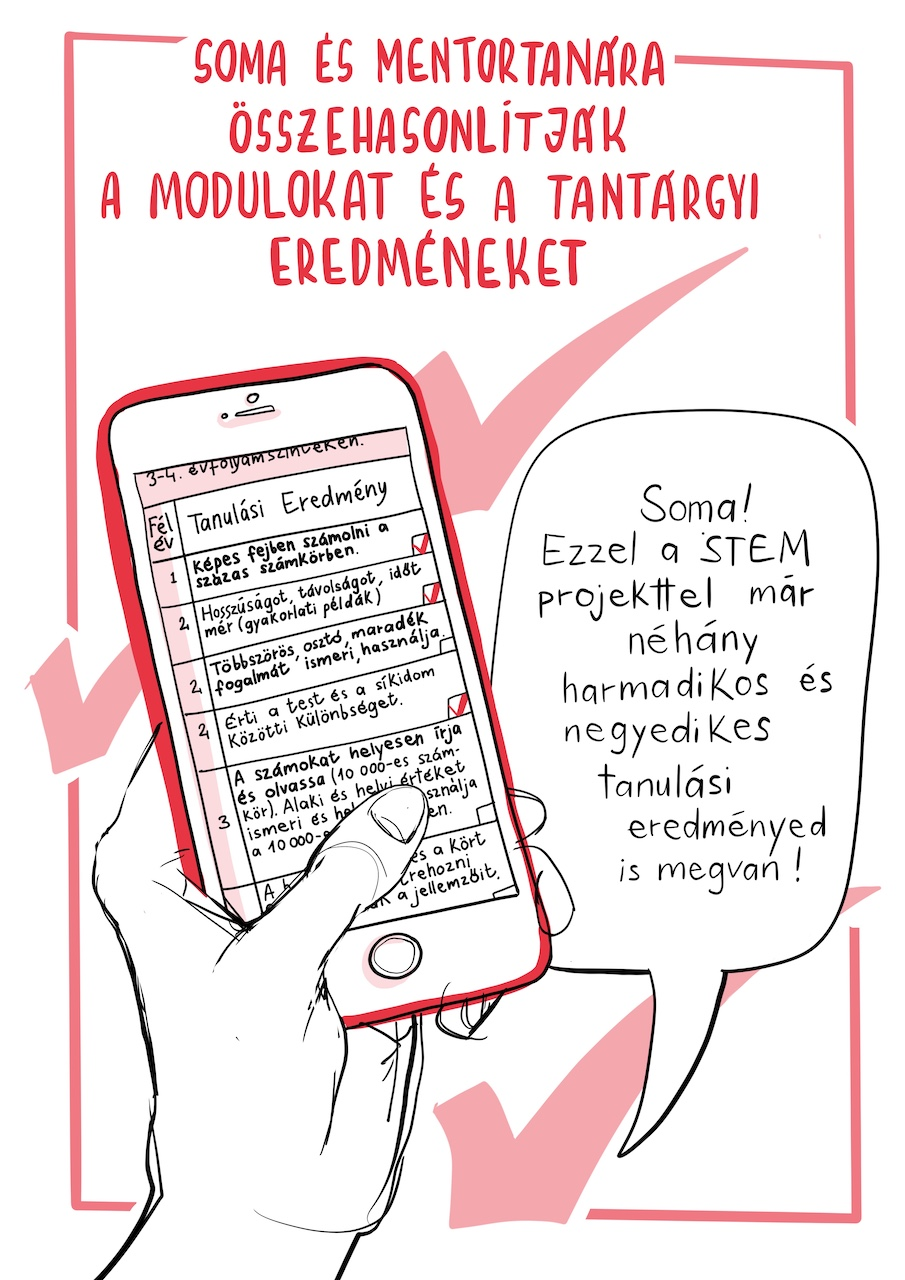
\includegraphics{pics/6a_tantargyi_soma.jpg}
\caption{Tanulási eredmények elszámolása}
\end{figure}

\hypertarget{uj-tanulasi-eredmenyek}{%
\paragraph{Új tanulási eredmények}\label{uj-tanulasi-eredmenyek}}

A gyerekek olyan tanulási eredményt is elérhetnek, ami a modulok céljai
között eredetileg nem volt megadva, mert

\begin{itemize}
\tightlist
\item
  lehetőségük van egyénileg is tanulni;
\item
  tanulási eredményekkel járnak a projektek, az iskolai lét, a közösségi
  élet és még számos informális és nem-formális tanulási helyzet;
\item
  egy modul során is alakulhatnak előre nem tervezett helyzetek,\break
  amik
  hozzásegíthetik a gyerekeket tanulási eredmények eléréséhez.
\end{itemize}

Az újonnan létrejövő tanulási eredmények is bekerülnek a portfólióba.

\hypertarget{tanulasi-eredmenyek-dokumentacioja}{%
\paragraph{Tanulási eredmények
dokumentációja}\label{tanulasi-eredmenyek-dokumentacioja}}

Minden modult dokumentálni\break
kell, hogy annak célja, kitűzött eredményei
nyilvánosak legyenek a Budapest School valamennyi tanára számára, és ha
szükséges, újra meg lehessen hirdetni. A tanulási eredményeket a
modulhoz kapcsolódó terv---tény összehasonlítás alapján határozzuk
meg. Az elért eredmények újra elérhetők, amennyiben a
folyamatos fejlődés biztosítva van.

\hypertarget{egyseges-modulok-egyedi-alkalmazasa}{%
\paragraph{Egységes modulok egyedi
alkalmazása}\label{egyseges-modulok-egyedi-alkalmazasa}}

Egy modul elvégzésével a gyerekek más-más tanulási eredményt is elérhetnek.

\begin{itemize}
\tightlist
\item
  Működhet a differenciálás, tehát nem minden gyerek ugyanazt és
  ugyanúgy csinálja a foglalkozásokon. Egy modulban tud együtt tanulni
  az a gyerek, aki még a \emph{„Hangokból, szótagokból szavakat épít''}
  eredményért dolgozik, és az, aki \emph{„Értő figyelemmel követi a
  tanító, illetve társai felolvasását.''}
\item
  A modulnak része lehet testre szabható sáv is. Például egy tudományos
  kísérletező modulban néhány gyerek a rövid távú memória és a fáradtság
  kapcsolatát kutatja, a másik csoport az esőzés és a közlekedési dugók
  kialakulása közti kapcsolatot vizsgálja. Minden gyerek elérheti a
  \emph{„Megérti a környezetében jelen lévő logikai, mennyiségi,
  függvényszerű, térbeli és statisztikai kapcsolatokat''} (Matematika 9--12.) eredményt, de a két különböző kutató csapat más-más
  területen dolgozik, így más témában merül el.
\item
  Egy-egy gyerek saját tanulási célja érdekében extra lépéseket tehet,
  és olyan eredményeket is el tud érni, amit mások nem. Például egy
  modul végén önálló prezentációt, saját kutatási tervet vagy egy kész
  működő modellt alkothat.
\end{itemize}

\hypertarget{tanulasi-eredmenyek-elerese}{%
\subsection{Tanulási eredmények
elérése}\label{tanulasi-eredmenyek-elerese}}

A tanulási eredményt sokféleképpen tekinthetjük elértnek.

\begin{itemize}
\tightlist
\item
  A modulok végeztével a tanárok igazolhatják a tanulási eredmény
  elérését.
\item
  Kihívások, tudáspróbák, tesztek, szabványos vizsgák teljesítése
  szintén megadott tanulási eredmény elérést igazolja.
\end{itemize}

Az elért tanulási eredmények bekerülnek a portfólióba. Így mindig nyomon
követhető, hogy mi és ki igazolja a tanulási eredmény elérésének tényét.

\hypertarget{ha-nincsenek-meg-a-tanulasi-eredmenyek}{%
\paragraph{Ha nincsenek meg a tanulási
eredmények}\label{ha-nincsenek-meg-a-tanulasi-eredmenyek}}

Az elért tanulási eredmények listája a portfólióban bármikor bővíthető.
Egy feladatlap kitöltése, egy tudáspróba, egy vizsga (akár online
vizsga) mind-mind tanulási eredmények elérésének bizonyítékai. Ha a
portfólió alapján nem állapítható meg az évfolyam teljesítéséhez és az
osztályzathoz szükséges tanulási eredmények megléte, akkor a gyereknek
ki kell egészítenie a portfólióját.

Ugyancsak kiegészítendő a portfólió, ha igazolt vagy igazolatlan
mulasztások miatt az iskolában végzett munka nem volt elegendő az
elégséges portfólió-elemek összegyűjtésére. Ez azt is jelenti, hogy az
iskolának nem kell a fenti folyamattól, folyamatoktól eltérnie, csak a
portfóliót kell kibővíteni.

\hypertarget{evfolyam-osztalyzatok-bizonyitvany}{%
\section{Évfolyam, osztályzatok,
bizonyítvány}\label{evfolyam-osztalyzatok-bizonyitvany}}

A Budapest Schoolban tanuló gyerekek saját tanulási célokat tűznek ki,
tanulnak, alkotnak, trimeszterenként frissítik a portfóliójukat,
mentorukkal és a szaktanárokkal értékelik haladásukat, és ha kell,
újraterveznek.

Saját céljaik vannak, és sokszor a saját céljaik eléréséhez maguknak
kell felállítaniuk követelményeket. „Ha pszichológus akarok lenni, akkor
emeltszintű biológia érettségit kell tennem. Ehhez a mai tudásom alapján
nekem legalább hetente két órát kell a felkészüléssel foglalkoznom.''
Egyféle elvárásrendszer azonban adott a gyerek és az iskola számára, és
ez a Nemzeti Alaptanterv elvárásrendszere.

\hypertarget{evfolyam}{%
\subsection{Az évfolyam}\label{evfolyam}}

A Nemzeti Alaptanterv tantárgyanként megadott \emph{elvárt tanulási
eredményekkel} határozza meg, hogy mit kell a gyerekeknek megtanulniuk
ahhoz, hogy a NAT szerint is haladni tudjanak az 1. évfolyamtól a 12.
évfolyamig. Az iskola feladata a gyerekeknek ebben a haladásban segíteni
és a haladást nyomonkövetni. A BPS-iskolákban egy gyerek akkor éri el
egy tantárgy adott évfolyamhoz tartozó követelményeit, ha a NAT által
megadott tanulási eredmények legalább 41\%-át teljesíti. Ha a gyerek
az adott évfolyamhoz tartozó minden tantárgy követelményeit elérte,
akkor léphet következő évfolyamra.

\begin{quote}
A BPS modell az évfolyamokra úgy tekint, mint egy
% \href{https://en.wikipedia.org/wiki/Experience_point}
{szerepjáték
nehézségi szintjeire}: akkor léphet egy gyerek a következő szintre, ha
az évfolyamhoz köthető tantárgyi tanulási eredményekből eleget
összegyűjtött.
\end{quote}

\hypertarget{tanulasi-eredmenyek-evfolyamokra-es-felevekre-bontasa}{%
\paragraph{Tanulási eredmények évfolyamokra és félévekre
bontása}\label{tanulasi-eredmenyek-evfolyamokra-es-felevekre-bontasa}}

A BPS modell ---~a Nemzeti Alaptantervvel összhangban~--- több esetben
több évfolyamot átívelő szakaszokra adja meg a tanulási eredményeket. Ha
egy pedagógiai szakasz $H$ hosszúságú, és arra a szakaszra a Nemzeti
Alaptanterv $N$ tanulási eredményt határoz meg, akkor a program évente
$N/H$ tanulási eredmény elérését tekinti célnak mind a
$H$ évben.

Például a \emph{magyar nyelv és irodalom} tantárgyból 136 tanulási
eredményt kell elérni az első négy évfolyamon, ezért a program a
gyerekek számára az első évfolyamra 136$/$4~=~35 tanulási eredményt
elérését tűzi ki.

\hypertarget{folyamatos-es-egyertelmu-haladas}{%
\paragraph{Folyamatos és egyértelmű
haladás}\label{folyamatos-es-egyertelmu-haladas}}

Mivel a BPS visszajelző rendszere folyamatos és rendszeres visszajelzést
szorgalmaz, ezért a gyerekek a tanév közben is „gyűjtik'' a tanulási
eredményeket a
portfóliójukba (\ref{portfolio}.~fejezet, \pageref{portfolio}.~oldal).
Ennek alapján tanév közben nemcsak a gyerek, hanem a tanárai és a családja is
mindig nyomon követhetik, hogy hol tart a gyerek, és mit kell tenni azért,
hogy a tanév végére elérje a az évfolyamhoz tartozó követelményeket.

\hypertarget{kevert-korosztaly-es-az-evfolyamok}{%
\paragraph{A kevert korosztályok és az
évfolyamok}\label{kevert-korosztaly-es-az-evfolyamok}}

A gyerekek a BPS-iskolákban sokszor vannak náluk fiatalabb vagy épp
idősebb gyerekekkel. Sokszor, sokféle csoportbontásban dolgoznak:
ugyanaz a két gyerek, aki együtt, egy csoportban tanul angolul,
lehet, hogy külön tanul matematikáról, mert teljesen máshol tartanak
a megértésben. Így az a kérdés, hogy \emph{„hányadikos vagy?''}, nem
annyira releváns a mindennapi tanulásban, mint az, hogy \emph{,,mit tanulsz épp?''}

\begin{figure}
\centering
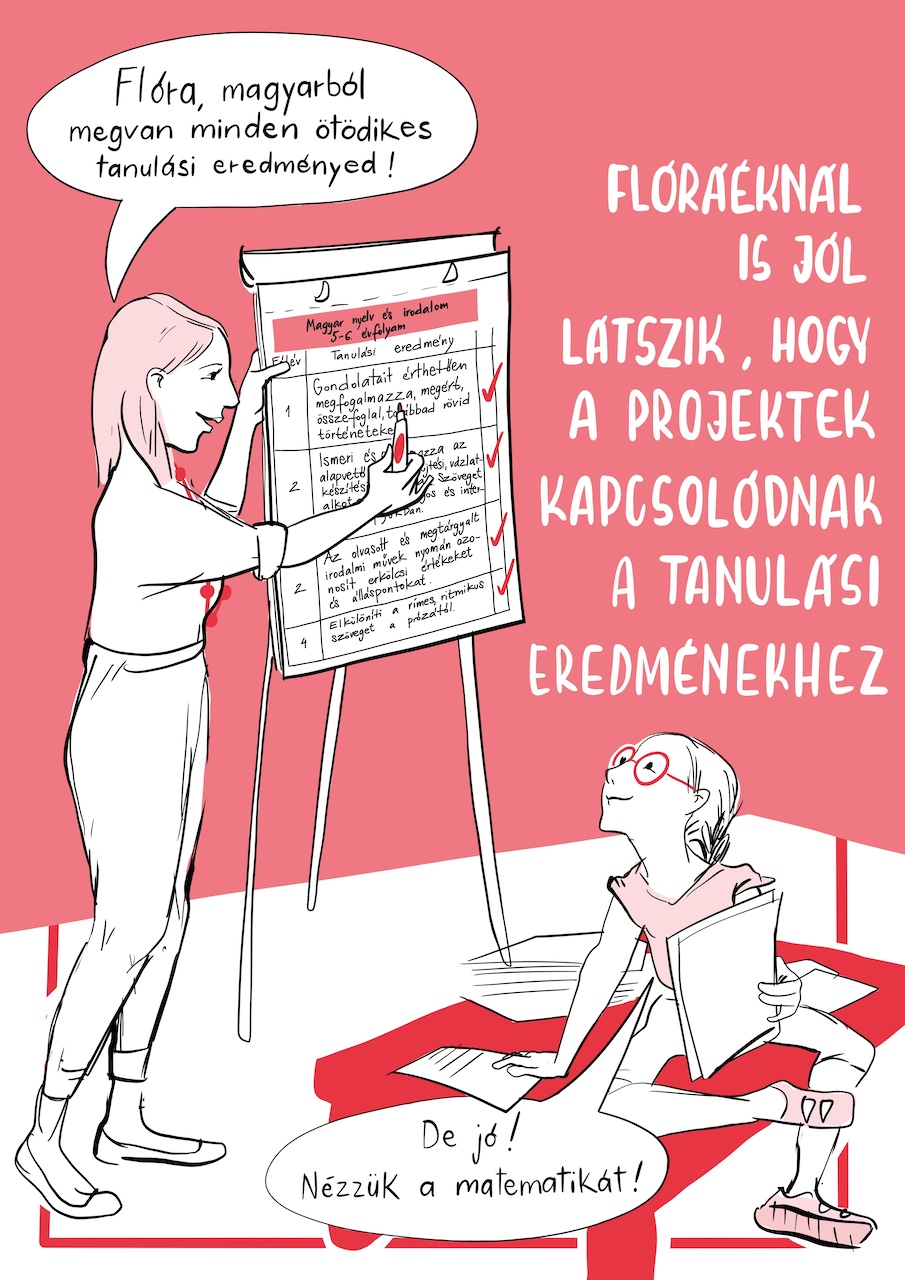
\includegraphics{pics/6b_tantargyi_flora.jpg}
\caption{Tanulási eredmények elszámolása}
\end{figure}

\hypertarget{erdemjegyek-es-osztalyzatok}{%
\subsection{Érdemjegyek és
osztályzatok}\label{erdemjegyek-es-osztalyzatok}}

Az Nkt.54.§ (1) szerint az érdemjegyek a tanév közben kapott 1--5 számok,
amik folyamatosan és rendszeresen értékelik a gyerek
\emph{teljesítményét és előmenetelét}.

A BPS modell folyamatos, többszempontú visszajelzést szorgalmaz, azaz
\emph{az érdemjegyek szerepét átveszik a többszempontú értékelő táblázatok
és visszajelzések}, illetve \emph{a tanulási eredmények elszámolása}. A
visszajelzésnek (\ref{visszajelzes-ertekeles}.~fejezet, \pageref{visszajelzes-ertekeles}.~oldal)
alaposnak, specifikusnak, többszempontúnak, a folyamatra fókuszálónak
kell lennie. Ezt a szerepet egy 1-től 5-ig terjedő skála önmagában nem
tudja ellátni.

\hypertarget{osztalyzatok-kialakitasa}{%
\subsubsection{Osztályzatok
kialakítása}\label{osztalyzatok-kialakitasa}}

Tantárgyankénti osztályzatok csak a NAT szerinti tantárgyi tudást,
teljesítményt és előmenetelt értékelhetik, és kizárólag a tanulási
eredmények elszámolásával alakulnak ki.

A gyerekek bármikor elérhetnek egy tanulási eredményt, aminek ténye
bekerül a portfóliójukba. Egy tanulási eredményt vagy teljesített a
gyerek, vagy nem, részben teljesíteni nem lehetséges. A teljesítés
igazolásának szabályait az iskola SZMSZ-e szabályozza.

Az elért tanulási eredmények osztályzatra váltásának a módja a
következő:

\begin{itemize}
\tightlist
\item
  Vesszük a félévben, illetve év végén a teljes évben elért tanulási
  eredmények számát, tehát a gyerek által az adott félévben\slash évben
  teljesített tanulási eredmények számosságát.
\item
  Ezt elosztjuk a BPS modell elvárt tantárgyi tanulási eredményeinek
  számával, és megszorozzuk 100-zal.
\item
  A kapott százalékos mutatót az alábbi táblázat alapján osztályzattá
  alakítjuk:
\end{itemize}

\begin{longtable}[]{@{}ll@{}}
% \toprule
\bfseries Teljesítmény &\bfseries Osztályzat\tabularnewline
\midrule
\endhead
0 - 40\% & 1\tabularnewline
41 - 50\% & 2\tabularnewline
51 - 60\% & 3\tabularnewline
61 - 70\% & 4\tabularnewline
71 - 100\% & 5\tabularnewline
\bottomrule
\end{longtable}

Az Ntk. előírja a tanuló magatartásának és szorgalmának
értékelését és minősítését. Ezt a gyerek mentora trimeszterenként
szövegesen vagy értékelő táblázatokban adja át.

\hypertarget{osztalyozo-vizsga}{%
\subsection{Osztályozó vizsga}\label{osztalyozo-vizsga}}

Az évfolyamok teljesítésének és az osztályzatok megítélésének folyamata a
gyerek évközi alkotásait, munkáját, teljesítményét tartalmazó
portfólió alapján történik, ezért a folyamat megfelel a
20/2012.(VIII.31.) EMMI-rendelet 64.~§ (1) azon elvárásának, hogy a
tanuló osztályzatait \emph{„évközi teljesítménye és érdemjegyei''}
alapján kell megállapítani, azzal a megkötéssel, hogy a BPS modell
elfogadja az érdemjegyeknél gazdagabb szöveges és értékelőtáblázat-alapú
visszajelzést.

Ha a portfólió alapján nem állapítható meg az évfolyamszintlépéshez és
az osztályzathoz szükséges tanulási eredmények megléte, akkor a
gyereknek ki kell egészítenie a portfólióját. Ez történhet akár egy
tudáspróbával vagy egy online teszttel is. Vagy el kell fogadnia, hogy
\emph{még} nem érte el a következő évfolyamszintre lépéshez szükséges
tanulási eredményeket.

Ugyancsak kiegészítendő a portfólió, ha igazolt vagy igazolatlan
mulasztások miatt az iskolában végzett munka nem volt elegendő az
elégséges portfólió-elemek összegyűjtésére. Ez azt is jelenti, hogy az
iskolának nem kell a fenti folyamattól, folyamatoktól eltérnie, csak a
portfóliót kell kibővíteni, vagy a gyereknek el kell
fogadnia, hogy \emph{még} nem érte el a következő évfolyamszintre
lépéshez szükséges tanulási eredményeket.

Ha a gyereket bármely okból felmentették a tanórai foglalkozásokon való
részvétel alól, akkor a 20/2012.(VIII.31.) EMMI-rendelet 64.~§ (2)
alapján osztályozóvizsgát kell tennie. Az iskolában az osztályozó vizsga
a tanulási eredmények vizsgakörülmények közötti igazolása.

\hypertarget{tankonyvek-kivalasztasa}{%
\section{Tankönyvek kiválasztása}\label{tankonyvek-kivalasztasa}}

A szaktanárok minden esetben maguk választják a modulhoz szükséges
tankönyveket, szoftvereket, weboldalakat és egyéb eszközöket úgy, hogy

\begin{itemize}
\tightlist
\item
  az megfelelő legyen annak a csoportnak, arra a célra, amit el akar
  érni;
\item
  minden esetben legyen mindenki számára elérhető (az esetek többségében
  értsd: ingyenes) megoldás;
\item
  a szaktanárokat bátorítjuk arra, hogy új dolgokat próbáljanak ki,
  és tapasztalataikat az iskola többi tanárával osszák meg.
\end{itemize}

Mivel az iskolában a NAT-ban és a miniszter által közreadott kerettantervben
meghatározott tanulási eredményeket kell elérni, az ehhez szükséges
ismeretek megszerzéséhez a Budapest School az Oktatási Hivatal általi
jegyzékben államilag támogatott, OFI által fejlesztett tankönyveket
veszi alapul. A Budapest School tanárcsapatainak lehetőségük van arra,
hogy ettől eltérő, a mindenkori tankönyvjegyzékben szereplő tankönyvvel
segítsék a tanulási eredmények elérését. És arra is lehetőségük van, hogy
egyáltalán ne használjanak tankönyvet, mert sokszor az internet elegendő
információt tartalmaz.

A Budapest School programjának alapja, hogy a gyerekek egyéni céljaira
szabott tanulási terveket készít. Ennek előfeltétele, hogy a könyvek
használata is ehhez kapcsolódó módon, rugalmasan történjen, minden
esetben az adott tanulási modul igényeihez szabva. Ennek érdekében a
program pedagógusai folyamatosam állítják össze a gyerekek eltérő
céljaihoz és képességszintjeihez igazodó differenciált tevékenységek és
feladatsorok rendszerét.

A Budapest School-iskolákban minden (modul)csoport csak olyan\break
tankönyvet választhat, amelyik minden család számára elérhető. Ha valamelyik család
nem tudja a könyvet magának megvásárolni, akkor a csoport többi tagja
megvásárolja neki.

\hypertarget{erettsegire-keszules}{%
\section{Érettségire készülés}\label{erettsegire-keszules}}

A BPS-ben a helyi tantervben szereplő tantárgyakból lehet középszintű
érettségit tenni.

Az emelt szintű érettségire fakultációs órák felvételével lehet
felkészülni. A BPS az emelt szintű érettségire való felkészítést a
következő tantárgyakból vállalja: magyar nyelv és irodalom, történelem,
matematika, digitális kultúra, fizika, biológia, földrajz, angol,
spanyol, német és testnevelés.

\hypertarget{az-egeszseges-es-boldog-gyerek}{%
\section{Az egészséges és boldog
gyerek}\label{az-egeszseges-es-boldog-gyerek}}

A Budapest School-gyerekek boldogak, egészségesek, hasznosak
közösségüknek. Képesek önmaguknak célokat állítani, azokat elérni.
Képesek már kisgyerekkortól sajátjukként megélni a tanulást, és ahhoz
kapcsolódóan célokat elérni, és fokozatosan tanulják meg azt, hogy
egyénileg és csoportosan is tudnak nagyszabású projekteket véghezvinni.
Tesznek a saját egészségükért, jövőjükért, társaikért, kapcsolódnak
önmagukhoz és társaikhoz.

A gyerekek személyiségfejődését két szinten támogatja az iskola. Az első
szintet a mindennapi működés adja, mert az iskola működése önmagában
személyiség- és egészségfejlesztő hatással bír. A második szintet a
\emph{harmónia} kiemelt fejlesztési irányelv biztosítja, ami holisztikus
megközelítésével támogatja a gyerekek fizikai, lelki jóllétét és
kapcsolódásukat a környezethez.

\hypertarget{mukodesbol-adodo-fejlesztesek}{%
\subsection{A működésből adódó
fejlesztések}\label{mukodesbol-adodo-fejlesztesek}}

Az iskola alapműködése, hogy a gyerekek csoportban, közösségben élnek,
tanulnak, dolgoznak, ezért „természetes'', hogy fejlődik az
\emph{empátiájuk, kooperációs, kollaborációs képességük és érzelmi
intelligenciájuk}. Alapelvünk: minél közelebb áll az iskola működése
a jövő hétköznapjaihoz, a családhoz és a munkahelyhez, annál jobban
támogatja a boldog
családi életre, a sikeres munkahelyre való felkészülést már önmagában az iskolában
való aktív részvétel is. Ehhez hasonlóan a támogató,
funkcionális, boldog családban felnőtt gyerekek nagyobb valószínűséggel
lesznek maguk is egészségesebbek és boldogabbak.

A \emph{fejlődésfókuszú gondolkodásmód} kialakítását kulcstényezőnek
gondoljuk a gyerekeink hosszú távú boldogulásához. Ezért az iskolában a saját célok
által irányított tanulási környezettől kezdve a jutalmazás, értékelés,
visszajelzés módjáig minden azt a célt szolgálja, hogy a
gyerekek képesek legyenek pozitívan gondolkodni magukról, ami az
ép és egészséges embernek talán egyik legfontosabb jellemzője.

A \emph{teljes körű iskolai egészségfejlesztést} az alábbi négy
egészségfejlesztési feladat rendszeres végzése adja:

\begin{itemize}
\tightlist
\item
  az egészséges táplálkozás megvalósítása (elsősorban megfelelő, magas
  minőségű, lehetőleg helyi alapanyagokból);
\item
  mindennapi testmozgás minden gyereknek (változatos foglalkozásokkal,
  koncentráltan az egészségjavító elemekre, módszerekre, pl. tartásjavító
  torna, tánc, jóga);
\item
  a gyerekek érett személyiséggé válásának elősegítése személyközpontú
  pedagógiai módszerekkel és a művészetek személyiségfejlesztő
  hatékonyságú alkalmazásával (ének, tánc, rajz, mesemondás, népi
  játékok, stb.);
\item
  a környezeti, médiatudatossági, fogyasztóvédelmi, balesetvédelmi\break
  egészségfejlesztési modulok, modulrészletek hatékony (azaz
  ,,bensővé váló'') oktatása.
\end{itemize}

\hypertarget{egeszsegugyi-felmeres-szervezese-es-hatasa-a-gyerekek-eletere}{%
\subsection{Egészségügyi felmérések szervezése és ezek hatása a gyerekek
életére}\label{egeszsegugyi-felmeres-szervezese-es-hatasa-a-gyerekek-eletere}}

A Budapest School-gyerekek megelőző jelleggel rendszeresen iskolaorvosi,
védőnői és fogorvosi felülvizsgálaton vesznek részt. Az orvosi, védőnői
és fogorvosi vizsgálatot a fenntartó a mindenkori jogszabályokban
meghatározott rendszerességgel szervezi meg. Jelenleg ezeket külső
helyszínen, megbízott orvossal, fogorvossal és védőnővel szervezi meg a
fenntartó.

Minden tanulóközösség tanulásszervező csapata a tanév megkezdése előtt
kijelöli az egészségnapokat: amikor a védőnői, orvosi, fogorvosi és
egyéb fizikai és mentális felülvizsgálatokat megszervezi. Húsz főig egy,
afölött pedig két napot kell megjelölni és a fenntartóval egyeztetni.
Egyeztetni azért kell, hogy a különböző tanulóközösségek között ne
legyen időpontütközés. Ha a gyerek az egészségnapon hiányzik az
iskolából, akkor a szülő feladata a felülvizsgálatot megszerveznie.

Ezeken a napokon a gyerekek és a tanárok iskolaidőben elutaznak a
rendelőkbe, felkeresik az orvost, fogorvost, védőnőt. Mivel a gyerekek
kivizsgálása feltehetőleg egyesével történik, az éppen nem soron levőknek
sokat kell várniuk. Ezért a tanárok erre az időre
mikromodulokat terveznek az egészség témájában.  Ilyenkor a gyerekek olyan tanulási eredményeket
érhetnek el, mint a \emph{„Tisztában van az egészség megőrzésének
jelentőségével, és tudja, hogy maga is felelős ezért''} (5. évfolyam 1.
félév).

A felülvizsgálatok eredményeit a gyerekek a mentorokkal megbeszélik,
és ha szükséges, akkor az eredmények alapján fejlődési célokat
fogalmaznak meg. A vizsgálatok eredményeit a gyerekek a portfóliójukban\break
ugyanúgy megőrzik, mint például egy tudáspróba eredményét.

\hypertarget{mindennapos-testmozgas}{%
\section{Mindennapos testmozgás}\label{mindennapos-testmozgas}}

Az iskolában „tanulóközösségek saját fókuszuk, helyszínük, stílusuk
alakulhat ki''. Ennek részeként a gyerekek mindennapos testmozgását is a
tanulóközösségenként másképp, az identitásuk és lehetőségeik szerint
alakítják ki. Az iskola csak annyit ír elő, hogy mindennap legyen
minimum 35 perc, aminek elsődleges célja a testmozgás és testnevelés.

Nincs olyan testmozgásforma, amelyet ez a program preferálna, vagy amely
kizárt lenne. A mindennapos testmozgás fizikai szükségleteinek
megszervezése is változatos módon történhet:

\begin{enumerate}
\def\labelenumi{\arabic{enumi}.}
\item
  Egyes telephelyek saját tornatermében, tornaszobájában vagy udvarán.
\item
  Szerződés, megállapodás alapján, elérhető közelben lévő más oktatási
  vagy sportlétesítményben (úszás, korcsolya, torna, foci, falmászás,
  sípálya).
\item
  A szabadban, épített helyszínhez nem kötődő mozgásszervezés (pl.
  kirándulás, séta, barangolás, felfedező játékok).
\item
  A feladatellátási helyeken, magyarul a tantermekben, speciálisan
  sportra alkalmas helyiséget nem igénylő mozgások esetén (pl. jóga).
\end{enumerate}

A testmozgás minden esetben a mozgást ismerő, abban képesítéssel,
végzettséggel vagy megfelelő gyakorlattal rendelkező személy vezetésével
vagy felügyelete mellett zajlik. Az iskola feladata monitorozni a
mindennapos testnevelés megvalósulását: ki, mikor, hol, milyen
testmozgást vezetett a gyerekeknek.

\hypertarget{elsosegely-nyujtasi-alapismeretek}{%
\section{Elsősegélynyújtási
alapismeretek}\label{elsosegely-nyujtasi-alapismeretek}}

A cél, hogy a gyerekek és tanárok megtanulják aktívan úgy alakítani
környezetüket és viselkedésüket, hogy a balesetek számát minimalizálják,\break
hogy felismerjék, amikor segítségre van szükség, hogy hatékonyan
segítsenek, és tudjanak segítséget hívni. Ehhez gyakorlásra, a témával
kapcsolatos védett időre van szükség. Ezért a 2., 4., 6., 8. és
10. évfolyam csak akkor teljesíthető, ha a gyerek minden második évben
elvégez egy minimum négyórás modult, aminek célja,

\begin{itemize}
\tightlist
\item
  hogy a gyerekek sajátítsák el a legalapvetőbb és legkorszerűbb
  elsősegélynyújtási módokat, azaz tudjanak egymásnak segíteni
  baj esetén (nemcsak elméletben, hanem a gyakorlatban is);
\item
  sajátítsák el, mikor és hogyan kell mentőt, segítséget hívni;
\item
  foglalkozzanak azzal, hogy hogyan tudják környezetüket, csoportjukat,
  tanulóközösségüket biztonságosabbá tenni, és ezt dokumentálják is.
\end{itemize}

A modul szervezője próbáljon meg elsősegélynyújtási bemutatót szervezni
a gyerekeknek az Országos Mentőszolgálat, a Magyar Ifjúsági Vöröskereszt,
az Ifjúsági Elsősegélynyújtók Országos Egyesülete szakembereinek vagy más,
magyar vagy külföldi képesítést szerzett szakembernek a bevonásával.

Az elsősegélynyújtási alapismeretek elsajátításával kapcsolatos
feladatok megvalósításának elősegítése érdekében az iskola

\begin{itemize}
\item
  kapcsolatot épít ki az Országos Mentőszolgálattal, a Magyar Ifjúsági
  Vöröskereszttel vagy az Ifjúsági Elsősegélynyújtók Országos
  Egyesületével. Tanulóink ---~választásuk szerint~--- bekapcsolódhatnak
  az elsősegélynyújtással kapcsolatos iskolán kívüli vetélkedőkbe;
\item
  minden második évben legalább egyszer a tanároknak lehetőséget
  biztosít elsősegély-tanfolyam látogatására.
\end{itemize}

\hypertarget{onkentes-kozossegi-szolgalat}{%
\section{Önkéntes közösségi
szolgálat}\label{onkentes-kozossegi-szolgalat}}

Az Nkt 4.~§ (15) pontjában definiált közösségi szolgálatot is modulként
hirdetjük meg, amit csak a 12.~évét már betöltött gyerek választhat.
Közösségi szolgálatként elfogadható, ha a Budapest School iskola egy
másik tanulóközösségében segít a gyerek.

\vspace*{-.8ex}
\hypertarget{nemzetisegek-megismerese}{%
\section{Nemzetiségek megismerése}\label{nemzetisegek-megismerese}}

Az iskola környezetében élő nemzetiségek kultúrájának megismerését
fontosnak tartja az iskola. Ezért minden második tanévben a településen
működő nemzetiségi önkormányzatokkal kapcsolatot vesz fel, és velük
együttműködve legalább 4 órás modulokat alakít ki. A modulok célja, hogy
a modul résztvevői megismerjék a nemzetiségekről azt, amit az
önkormányzatok fontosnak tartanak megmutatni.

Minden második évben legalább három önkormányzattal három különböző
modult kínál fel az iskola választásra. Amelyik településen ennél több
nemzetiségi önkormányzat működik, ott a tanév megkezdése előtt,
augusztus folyamán véletlenszerűen sorsoljuk ki az adott évi 3
megismerendő nemzetiséget.

\vspace*{-.8ex}
\hypertarget{kornyezeti-neveles}{%
\section{Környezeti nevelés}\label{kornyezeti-neveles}}

Ahogy az UNESCO 1977-ben meghatározta: \emph{„a környezeti nevelés olyan
folyamat, melynek célja, hogy a világ népessége környezettudatosan
gondolkodjék, figyeljen oda a környezetre és minden azzal kapcsolatos
problémára. Rendelkezzen az ehhez szükséges tudással, beállítódással,
képességekkel, motivációval, valamint mind egyéni, mind közösségi téren
eltökélten törekedjék a jelenlegi problémák megoldására és az újabbak
megelőzésére''}.

A környezeti nevelés céljainak eléréséhez a tanárok
környezettudatosságára, rendszerszemléletére és aktív részvételére van
szükség. Ezért az iskola vállalja, hogy a tanárainak tanévente legalább
4 órás workshopot szervez a témában, ahol a tanárok arról is tudnak
beszélni, hogyan vitték be a környezeti nevelést a gyerekek
mindennapjaiba.

% \hypertarget{tantargyak-tartalma-a-tanulasi-eredmenyek}{%
\section{Tantárgyak tartalma, a tanulási
eredmények}\label{tantargyak-tartalma-a-tanulasi-eredmenyek}}

\hypertarget{allampolgari-ismeretek}{%
\subsection{Állampolgári ismeretek}\label{allampolgari-ismeretek}}

\hypertarget{evfolyamon}{%
\subsubsection{8. évfolyamon}\label{evfolyamon}}

\begin{itemize}
\item
  Megérti a család, mint a társadalom alapvető intézményének szerepét,
  és értelmezi jellemzőit.
\item
  Lokálpatriotizmusa megerősödik, személyiségébe beépülnek a nemzeti
  közösséghez tartozás, a hazaszeretet emocionális összetevői.
\item
  Ismeri a demokratikus jogállam működésének alapvető sajátosságait,
  alapvető kötelezettségeit.
\item
  Jártasságot szerez mindennapi ügyeinek intézésében.
\item
  Saját pénzügyeiben tudatos döntéseket hoz.
\item
  Értelmezi a család mint a társadalom alapvető intézményének szerepét
  és jellemzőit.
\item
  Értelmezi a családi kohézió alapelemeit, jellemzőit: együttműködés,
  szeretetközösség, kölcsönösség, tisztelet.
\item
  Felismeri a családi szocializációnak az ember életútját befolyásoló
  jelentőségét.
\item
  Ismeri a magyar állam alapvető intézményeinek feladatkörét és
  működését.
\item
  Értelmezi a törvényalkotás folyamatát.
\item
  Ismeri a saját településének, lakóhelyének alapvető jellemzőit,
  értelmezi a településen működő intézmények és szervezetek szerepét és
  működését.
\item
  A lakóhelyével kapcsolatos javaslatokat fogalmaz meg, tervet készít a
  település fejlesztésének lehetőségeiről.
\item
  Felismeri a jogok és kötelességek közötti egyensúly kialakításának és
  fenntartásának fontosságát, megismeri a haza iránti kötelezettségeit,
  feladatait.
\item
  Ismeri településének, lakóhelyének kulturális, néprajzi értékeit, a
  település történetének alapvető eseményeit és fordulópontjait.
\item
  Megfogalmazza a nemzeti identitás jelentőségét az egyén és a közösség
  szempontjából is.
\item
  Felismeri a nemzetek, nemzetállamok fontosságát a globális világban.
\item
  Megismeri és értelmezi a honvédelem jelentőségét, feladatait és
  szerepét.
\item
  Azonosítja a mindennapi ügyintézés alapintézményeit, az alapvető
  ellátó rendszerek funkcióját és működési sajátosságait.
\item
  Azonosítja az igazságszolgáltatás intézményeit és működésük
  jellemzőit, megismeri az alapvető ellátórendszereket és funkcióikat.
\item
  Megismeri és értelmezi a diákmunka alapvető jogi feltételeit,
  kereteit.
\item
  Információkat gyűjt és értelmez a foglalkoztatási helyzetről, a
  szakmaszerkezet változásairól.
\item
  Ismeri a családi háztartás összetevőit, értelmezi a család
  gazdálkodását meghatározó és befolyásoló tényezőket.
\item
  Felismeri a családi háztartás gazdasági-pénzügyi fenntarthatóságának
  és a környezettudatos életvitel kialakításának társadalmi
  jelentőségét.
\item
  Értelmezi az állam gazdasági szerepvállalásának területeit.
\item
  Felismeri a közteherviselés gazdasági, társadalmi és erkölcsi
  jelentőségét, a társadalmi felelősségvállalás fontosságát.
\item
  Fogyasztási szokásaiban érvényesíti a tudatosság szempontjait is.
\item
  Felismeri a véleménynyilvánítás, érvelés, a párbeszéd és a vita
  társadalmi hasznosságát.
\item
  Képes arra, hogy feladatai egy részét a társas tanulás keretében
  végezze el.
\item
  Önállóan vagy társaival együttműködve javaslatokat fogalmaz meg,
  tervet, tervezetet készít.
\item
  Önállóan vagy segítséggel használja az infokommunikációs eszközöket.
\end{itemize}

\hypertarget{evfolyamon-1}{%
\subsubsection{12. évfolyamon}\label{evfolyamon-1}}

\begin{itemize}
\item
  Megérti a család szerepét, alapvető feladatait az egyén és a nemzet
  szempontjából egyaránt.
\item
  Értékeli a nemzeti identitás jelentőségét az egyén és a közösség
  szempontjából is.
\item
  Ismeri a választások alapelveit és a törvényhozás folyamatát.
\item
  Megismeri a demokratikus jogállam működésének alapvető sajátosságait.
\item
  Érti és vallja a haza védelmének, a nemzetért történő tenni akarás
  fontosságát.
\item
  A mindennapi életének megszervezésében alkalmazza a jogi és
  gazdasági-pénzügyi ismereteit.
\item
  Saját pénzügyeiben tudatos döntéseket hoz.
\item
  Felismeri az életpálya-tervezés és a munkavállalás egyéni és
  társadalmi jelentőségét.
\item
  Ismeri a munka világát érintő alapvető jogi szabályozást, a
  munkaerőpiac jellemzőit, tájékozódik a foglalkoztatás és a
  szakmaszerkezet változásairól.
\item
  Értelmezi a család mint a társadalom alapvető intézményének szerepét
  és jellemzőit.
\item
  Társaival megbeszéli a párválasztás, a családtervezés fontos
  szakaszait, szempontjait és a gyermekvállalás demográfiai
  jelentőségét: tájékozódás, minták, orientáló példák, átgondolt
  tervezés, felelősség.
\item
  Felismeri, hogy a családtagok milyen szerepet töltenek be a
  szocializáció folyamatában.
\item
  Értelmezi a családi szocializációnak az ember életútját befolyásoló
  jelentőségét.
\item
  Felismeri az alapvető emberi jogok egyetemes és társadalmi
  jelentőségét.
\item
  Bemutatja magyarország alaptörvényének legfontosabb részeit:
  alapvetés; az állam; szabadság és felelősség.
\item
  Érti a társadalmi normák és az egyéni cselekedetek, akaratok, célok
  egyeztetésének, összehangolásának követelményét. elméleti és
  tapasztalati úton ismereteket szerez a társadalmi
  felelősségvállalásról, a segítségre szorulók támogatásának
  lehetőségeiről.
\item
  Megérti a honvédelem szerepét az ország biztonságának fenntartásában,
  megismeri a haza védelmének legfontosabb feladatcsoportjait és
  területeit, az egyén kötelezettségeit.
\item
  Felismeri és értelmezi az igazságosság, az esélyegyenlőség
  biztosításának jelentőségét és követelményeit.
\item
  Értelmezi a választójog feltételeit és a választások alapelveit.
\item
  Értelmezi a törvényalkotás folyamatát.
\item
  Megérti a nemzeti érzület sajátosságait és a hazafiság fontosságát,
  lehetséges megnyilvánulási formáit.
\item
  Véleményt alkot a nemzetállamok és a globalizáció összefüggéseiről.
\item
  Felismeri a világ magyarsága mint nemzeti közösség összetartozásának
  jelentőségét.
\item
  Érti és felismeri a honvédelem mint nemzeti ügy jelentőségét.
\item
  Felismeri és értékeli a helyi, regionális és országos közgyűjtemények
  nemzeti kulturális örökség megőrzésében betöltött szerepét.
\item
  Azonosítja a mindennapi ügyintézés alapintézményeit.
\item
  Életkori sajátosságainak megfelelően jártasságot szerez a jog
  területének mindennapi életben való alkalmazásában.
\item
  Tájékozott a munkavállalással kapcsolatos szabályokban.
\item
  Megtervezi egy fiktív család költségvetését.
\item
  Saját pénzügyi döntéseit körültekintően, megalapozottan hozza meg.
\item
  Megismeri a megalapozott, körültekintő hitelfelvétel szempontjait,
  illetve feltételeit.
\item
  Azonosítja az állam gazdasági szerepvállalásának elemeit.
\item
  Felismeri és megérti a közteherviselés nemzetgazdasági, társadalmi és
  morális jelentőségét.
\item
  Életvitelébe beépülnek a tudatos fogyasztás elemei, életmódjában
  figyelmet fordít a környezeti terhelés csökkentésére, érvényesíti a
  fogyasztóvédelmi szempontokat.
\item
  Értelmezi a vállalkozás indítását befolyásoló tényezőket.
\item
  Felismeri a véleménynyilvánítás, érvelés, a párbeszéd és a vita
  társadalmi hasznosságát.
\item
  Képes arra, hogy feladatait akár önálló, akár társas tanulás révén
  végezze el, célorientáltan képes az együttműködésre.
\item
  Önállóan vagy társaival együttműködve javaslatokat fogalmaz meg.
\item
  Tiszteletben tartja a másik ember értékvilágát, gondolatait és
  véleményét, ha szükséges, kritikusan viszonyul emberi cselekedetekhez,
  magatartásformákhoz.
\item
  Megismerkedik a tudatos médiafogyasztói magatartással és a közösségi
  média használatával.
\item
  A tanulási tevékenységek szakaszaiban használja az infokommunikációs
  eszközöket, lehetőségeket, tisztában van azok szerepével, innovációs
  potenciáljával és veszélyeivel is.
\end{itemize}

\hypertarget{biologia}{%
\subsection{Biológia}\label{biologia}}

\hypertarget{evfolyamon-2}{%
\subsubsection{9-10. évfolyamon}\label{evfolyamon-2}}

\begin{itemize}
\item
  A mindennapi élettel összefüggő problémák megoldásában alkalmazza a
  természettudományos gondolkodás műveleteit, rendelkezik a biológiai
  problémák vizsgálatához szükséges gyakorlati készségekkel.
\item
  Az élő rendszerek belső működése és környezettel való kapcsolataik
  elemzésében alkalmazza a rendszerszintű gondolkodás műveleteit.
\item
  Életközösségek vizsgálata alapján értelmezi a környezet és az
  élőlények felépítése és működése közötti összefüggést, érti az
  ökológiai egyensúly jelentőségét, érvel a biológiai sokféleség
  megőrzése mellett.
\item
  Az emberi test és pszichikum felépítéséről és működéséről szerzett
  ismereteit önismeretének fejlesztésében, egészséges életvitelének
  kialakításában alkalmazza.
\item
  Felismeri a helyi és a globális környezeti problémák összefüggését,
  érvel a föld és a kárpát-medence természeti értékeinek védelme
  mellett, döntéseket hoz és cselekszik a fenntarthatóság érdekében.
\item
  Ismeri a biológiai kutatások alapvető céljait, legfontosabb
  területeit, értékeli az élet megértésében, az élővilág megismerésében
  és megóvásában játszott szerepét.
\item
  Példákkal igazolja a biológiai ismereteknek a világképünk és a
  technológia fejlődésében betöltött szerepét, gazdasági és társadalmi
  jelentőségét.
\item
  Az élő rendszerek vizsgálata során felismeri az analógiákat,
  korrelációkat, alkalmazza a statisztikus és a rendszerszintű
  gondolkodás műveleteit, kritikusan és kreatívan mérlegeli a
  lehetőségeket, bizonyítékokra alapozva érvel, több szempontot is
  figyelembe vesz.
\item
  A vizsgált biológiai jelenségek magyarázatára előfeltevést fogalmaz
  meg, ennek bizonyítására vagy cáfolatára kísérletet tervez és
  kivitelez, azonosítja és beállítja a kísérleti változókat,
  megfigyeléseket és méréseket végez.
\item
  Biológiai vonatkozású adatokat elemez, megfelelő formába rendez,
  ábrázol, ezek alapján előrejelzéseket, következtetéseket fogalmaz meg,
  a már ábrázolt adatokat értelmezi.
\item
  Egyénileg és másokkal együttműködve célszerűen és biztonságosan
  alkalmaz biológiai vizsgálati módszereket, ismeri a fénymikroszkóp
  működésének alapelvét, képes azt használni.
\item
  Érti a biológia molekuláris szintű vizsgálati módszereinek elméleti
  alapjait és felhasználási lehetőségeit, értékeli a biológiai
  kutatásokból származó nagy mennyiségű adat feldolgozásának
  jelentőségét.
\item
  A biológiai jelenségek vizsgálata során digitális szöveget, képet,
  videót keres, értelmez és felhasznál, vizsgálja azok megbízhatóságát,
  jogszerű és etikus felhasználhatóságát.
\item
  Biológiai vizsgálatok során elvégzi az adatrögzítés és -rendezés
  műveleteit, ennek alapján tényekkel alátámasztott következtetéseket
  von le.
\item
  Ismeri a tudományos közlések lényegi jellemzőit.
\item
  Tájékozódik a biotechnológia és a bioetika kérdéseiben, ezekről folyó
  vitákban tudományosan megalapozott érveket alkot.
\item
  A valós és virtuális tanulási közösségekben, másokkal együttműködve
  megtervez és kivitelez biológiai vizsgálatokat, projekteket.
\item
  Tudja a biológiai problémákat és magyarázatokat a megfelelő szinttel
  összefüggésben értelmezni.
\item
  Tényekkel bizonyítja az élőlények elemi összetételének hasonlóságát, a
  biogén elemek, a víz, az atp és a makromolekulák élő szervezetekben
  betöltött alapvető szerepét.
\item
  Megérti, miért és hogyan mehetnek végbe viszonylag alacsony
  hőmérsékleten, nagy sebességgel kémiai reakciók a sejtekben, vizsgálja
  az enzimműködést befolyásoló tényezőket.
\item
  Értékeli és példákkal igazolja a különféle szintű biológiai
  szabályozás szerepét az élő rendszerek normál működési állapotának
  fenntartásában.
\item
  Magyarázza, hogy a sejt az élő szervezetek szerkezeti és működési
  egysége.
\item
  Ábrák, animációk alapján értelmezi, és biológiai tényekkel
  alátámasztja, hogy a vírusok az élő és élettelen határán állnak.
\item
  A felépítés és működés összehasonlítása alapján bemutatja a sejtes
  szerveződés kétféle formájának közös jellemzőit és alapvető
  különbségeit, értékeli ezek jelentőségét.
\item
  Tényekkel igazolja a baktériumok anyagcsere sokfélesége, gyors
  szaporodása és alkalmazkodóképessége közötti összefüggést.
\item
  Felismeri az összetett sejttípus mikroszkóppal megfigyelhető
  sejtalkotóit, magyarázza a sejt anyagcsere-folyamatainak lényegét.
\item
  Ismeri az örökítőanyag többszintű szerveződését, képek, animációk
  alapján értelmezi a sejtekben zajló biológiai információ tárolásának,
  átírásának és kifejeződésének folyamatait.
\item
  Tudja, hogy a sejtekben és a sejtek között bonyolult jelforgalmi
  hálózatok működnek, amelyek befolyásolják a génműködést, és felelősek
  lehetnek a normál és a kóros működésért is.
\item
  Összehasonlítja a sejtosztódás típusait, megfogalmazza ezek biológiai
  szerepét, megérti, hogy a soksejtű szervezetek a megtermékenyített
  petesejt és utódsejtjei meghatározott számú osztódásával és
  differenciálódásával alakulnak ki.
\item
  Felismeri az összefüggést a rák kialakulása és a sejtciklus zavarai
  között, megérti, hogy mit tesz a sejt és a szervezet a daganatok
  kialakulásának megelőzéséért.
\item
  Ismeri az őssejt fogalmát, különféle típusait és azok jellemzőit,
  különbséget tesz őssejt és daganatsejt között.
\item
  Fénymikroszkópban, ábrán vagy fotón felismeri és jellemzi a főbb
  állati és növényi szövettípusokat, elemzi, hogy milyen funkciók
  hatékony elvégzésére specializálódtak.
\item
  Ismeri és példákkal bizonyítja az élőlények szén- és
  energiaforrásainak különféle lehetőségeit, az anyagcseretípusok
  közötti különbséget.
\item
  Vázlatrajzok, folyamatábrák és animációk alapján azonosítja a
  fotoszintézis és a sejtlégzés fő szakaszainak sejten belüli helyét és
  struktúráit, a fontosabb anyagokat és az energiaátalakítás jellemzőit.
\item
  A sejtszintű anyagcsere folyamatok alapján magyarázza a növények és
  állatok közötti ökológiai szintű kapcsolatot, a termelő és fogyasztó
  szervezetek közötti anyagforgalmat.
\item
  A földi élet keletkezését biológiai kísérletek és elméletek alapján
  magyarázza.
\item
  Érti és tényekkel igazolja az ősbaktériumok különleges élőhelyeken
  való életképességét.
\item
  Biológiai és csillagászati tények alapján mérlegeli a földön kívüli
  élet valószínűsíthető feltételeit és lehetőségeit.
\item
  Ismeri az örökítőanyag bázissorrendjének vagy bázisainak
  megváltozásához vezető folyamatokat, konkrét esetekben azonosítja ezek
  következményeit.
\item
  A géntechnológia céljának és módszertani alapjainak ismeretében,
  kritikai szemlélettel elemzi a genetikai módosítások előnyeit és
  kockázatait.
\item
  Érti az örökítőanyagban tárolt információ és a kifejeződő
  tulajdonságok közötti összefüggést, megkülönbözteti a genotípust és a
  fenotípust.
\item
  Megérti a genetikai információ nemzedékek közötti átadásának
  törvényszerűségeit, ezeket konkrét esetek elemzésében alkalmazza.
\item
  Felismeri a kapcsolatot az életmód és a gének kifejeződése között,
  érti, hogy a sejt és az egész szervezet jellemzőinek kialakításában és
  fenntartásában kiemelt szerepe van a környezet általi
  génaktivitás-változásoknak.
\item
  Megérti a természetes változatosság szerveződését, az evolúciós
  változások eredetét és elterjedését magyarázó elemi folyamatokat,
  felismer és magyaráz mikro- és makroszintű evolúciós jelenségeket.
\item
  Példákkal igazolja, hogy a szelekció a különböző szerveződési
  szinteken értelmezhető tulajdonságokon keresztül egyidejűleg hat.
\item
  Példákkal mutatja be az élővilág főbb csoportjainak evolúciós
  újításait, magyarázza, hogy ezek hogyan segítették elő az adott
  élőlénycsoport elterjedését.
\item
  Érti és elfogadja, hogy a mai emberek egy fajhoz tartoznak, és az
  evolúció során kialakult nagyrasszok értékükben nem különböznek, a
  biológiai és kulturális örökségük az emberiség közös kincse.
\item
  Morfológiai, molekuláris biológiai adatok alapján egyszerű
  származástani kapcsolatokat elemez, törzsfát készít.
\item
  Ismeri az evolúció befolyásolásának lehetséges módjait (például
  mesterséges szelekció, fajtanemesítés, géntechnológia), értékeli ezek
  előnyeit és esetleges hátrányait.
\item
  Megérti a környezeti állapot és az ember egészsége közötti
  összefüggéseket, azonosítja az ember egészségét veszélyeztető
  tényezőket, felismeri a megelőzés lehetőségeit, érvényesíti az
  elővigyázatosság elvét.
\item
  Elemzi az ember mozgásképességének biokémiai, szövettani és
  biomechanikai alapjait, ezeket összefüggésbe hozza a mindennapi élet,
  a sport és a munka mozgásformáival, értékeli a rendszeres testmozgás
  szerepét egészségének megőrzésében.
\item
  Az emberi test kültakarójának, váz- és izomrendszerének elemzése
  alapján magyarázza az ember testképének, testalkatának és
  mozgásképességének biológiai alapjait.
\item
  A táplálkozás-, a légzés-, a keringés- és a kiválasztás
  szervrendszerének elemzése alapján magyarázza az emberi szervezet
  anyag- és energiaforgalmi működésének biológiai alapjait.
\item
  Az ideg-, hormon- és immunrendszer elemzése alapján magyarázza az
  emberi szervezet információs rendszerének biológiai alapjait.
\item
  Felsorolja az emberi egyedfejlődés főbb szakaszait, magyarázza hogyan
  és miért változik a szervezetünk az életkor előrehaladásával, értékeli
  a fejlődési szakaszok egészségvédelmi szempontjait, önmagát is
  elhelyezve ebben a rendszerben.
\item
  Ismeri a férfi és a női nemi szervek felépítését és működését, a
  másodlagos nemi jellegeket és azok kialakulási folyamatát, ismereteit
  összekapcsolja a szaporító szervrendszer egészségtanával.
\item
  Biológiai ismereteit is figyelembe véve értékeli az emberi szexualitás
  párkapcsolattal és a tudatos családtervezéssel összefüggő
  jelentőségét.
\item
  Megérti a fogamzásgátlók hatékonyságáról szóló információkat, a
  személyre szabott, orvosilag ellenőrzött fogamzásgátlás fontosságát.
\item
  Ismeri a fogamzás feltételeit, a terhesség jeleit, bemutatja a magzat
  fejlődésének szakaszait, értékeli a terhesség alatti egészséges
  életmód jelentőségét.
\item
  A biológiai működések alapján magyarázza a stressz fogalmát, felismeri
  a tartós stressz egészségre gyakorolt káros hatásait, igyekszik azt
  elkerülni, csökkenteni.
\item
  Ismeri a gondolkodási folyamatokat és az érzelmi és motivációs
  működéseket meghatározó tényezőket, értékeli az érzelmi és az értelmi
  fejlődés kapcsolatát.
\item
  Ismeri a mentális egészség jellemzőit, megérti annak feltételeit, ezek
  alapján megtervezi az egészségmegőrző magatartásához szükséges
  életviteli elemeket.
\item
  Megérti az idegsejtek közötti jelátviteli folyamatokat, és kapcsolatba
  hozza azokat a tanulás és emlékezés folyamataival, a drogok
  hatásmechanizmusával.
\item
  Az agy felépítése és funkciója alapján magyarázza az információk
  feldolgozásával, a tanulással összefüggő folyamatokat, értékeli a
  tanulási képesség jelentőségét az egyén és a közösség szempontjából.
\item
  Biológiai folyamatok alapján magyarázza a függőség kialakulását,
  felismeri a függőségekre vezető tényezőket, ezek kockázatait és
  következményeit.
\item
  Ismeri az orvosi diagnosztika, a szűrővizsgálatok és védőoltások
  célját, lényegét, értékeli ezek szerepét a betegségek megelőzésében és
  a gyógyulásban.
\item
  Megkülönbözteti a házi- és a szakorvosi ellátás funkcióit, ismeri az
  orvoshoz fordulás módját, tisztában van a kórházi ellátás indokaival,
  jellemzőivel.
\item
  Ismeri a leggyakoribb fertőző betegségek kiváltó okait, ismeri a
  fertőzések elkerülésének lehetőségeit és a járványok elleni védekezés
  módjait.
\item
  Ismeri a leggyakoribb népbetegségek (pl. szívinfarktus, stroke,
  cukorbetegség, allergia, asztma) kockázati tényezőit, felismeri ezek
  kezdeti tüneteit.
\item
  Képes a bekövetkezett balesetet, rosszullétet felismerni,
\item
  Képes a sérült vagy beteg személy ellátását a rendelkezésre álló
  eszközökkel (vagy eszköz nélkül) megkezdeni, segítséget (szükség
  esetén mentőt) hívni.
\item
  Szükség esetén alkalmazza a felnőtt alapszintű újraélesztés műveleteit
  (cpr), képes a félautomata defibrillátort alkalmazni.
\item
  Példákkal mutatja be a fontosabb hazai szárazföldi és vizes
  életközösségek típusait, azok jellemzőit és előfordulásait.
\item
  Megfigyelések, leírások és videók alapján azonosítja a populációk
  közötti kölcsönhatások típusait, az ezzel összefüggő etológiai
  jellemzőket, bemutatja ezek jellegét, jelentőségét.
\item
  Érti az ökológiai mutatókkal, bioindikációs vizsgálatokkal megvalósuló
  környezeti állapotelemzések céljait, adott esetben alkalmazza azok
  módszereit.
\item
  Ismeri a levegő-, a víz- és a talajszennyezés forrásait, a szennyező
  anyagok típusait és példáit, konkrét esetek alapján elemzi az
  életközösségekre gyakorolt hatásukat.
\item
  Felismeri és példákkal igazolja az állatok viselkedésének a
  környezethez való alkalmazkodásban játszott szerepét.
\item
  Felismeri a természetes élőhelyeket veszélyeztető tényezőket, kifejti
  álláspontját az élőhelyvédelem szükségességéről, egyéni és társadalmi
  megvalósításának lehetőségeiről.
\item
  Érti a biológiai sokféleség fogalmát, ismer a meghatározásra alkalmas
  módszereket, értékeli a bioszféra stabilitásának megőrzésében játszott
  szerepét.
\item
  Érti az ökológiai egyensúly fogalmát, értékeli a jelentőségét,
  példákkal igazolja az egyensúly felborulásának lehetséges
  következményeit.
\item
  Érti az ökológiai rendszerek működése és a biológiai sokféleség
  közötti kapcsolatot, konkrét életközösségek vizsgálata alapján
  táplálkozási piramist, hálózatot elemez.
\item
  Konkrét példák alapján vizsgálja a bioszférában végbemenő
  folyamatokat, elemzi ezek idő- és térbeli viszonyait, azonosítja az
  emberi tevékenységgel való összefüggésüket.
\item
  A kutatások adatai és előrejelzései alapján értelmezi a globális
  éghajlatváltozás élővilágra gyakorolt helyi és bioszféra szintű
  következményeit.
\item
  Példák alapján elemzi a levegő-, a víz- és a talajszennyeződés, az
  ipari és természeti katasztrófák okait és ezek következményeit, az
  emberi tevékenységnek az élőhelyek változásához vezető hatását, ennek
  alapján magyarázza egyes fajok veszélyeztetettségét.
\item
  Érti és elfogadja, hogy a jövőbeli folyamatokat a jelen cselekvései
  alakítják, tudja, hogy a folyamatok tervezése, előrejelzése
  számítógépes modellek alapján lehetséges.
\item
  Értékeli a környezet- és természetvédelem fontosságát, megérti a
  nemzetközi összefogások és a hazai törekvések jelentőségét,
  döntéshozatalai során saját személyes érdekein túl a természeti
  értékeket és egészség-megőrzési szempontokat is mérlegeli.
\item
  Történeti adatok és jelenkori esettanulmányok alapján értékeli a
  mezőgazdaság, erdő- és vadgazdaság, valamint a halászat természetes
  életközösségekre gyakorolt hatását, példák alapján bemutatja az
  ökológiai szempontú, fenntartható gazdálkodás technológiai
  lehetőségeit.
\item
  Megérti a biotechnológiai eljárások és a bionika eredményeinek
  alkalmazási lehetőségeit, értékeli az információs technológiák
  alkalmazásának orvosi, biológiai jelentőségét.
\item
  Érvel a föld, mint élő bolygó egyedisége mellett, tényekre alapozottan
  és kritikusan értékeli a természeti okokból és az emberi hatásokra
  bekövetkező változásokat.
\item
  Ismeri a kárpát-medence élővilágának sajátosságait, megőrzendő
  értékeit, ezeket összekapcsolja a hazai nemzeti parkok
  tevékenységével.
\end{itemize}

\hypertarget{digitalis-kultura}{%
\subsection{Digitális kultúra}\label{digitalis-kultura}}

\hypertarget{evfolyamon-3}{%
\subsubsection{4. évfolyamon}\label{evfolyamon-3}}

\begin{itemize}
\item
  Elmélyülten dolgozik digitális környezetben, önellenőrzést végez.
\item
  Megvizsgálja és értékeli az általa vagy társai által alkalmazott,
  létrehozott, megvalósított eljárásokat.
\item
  Társaival együttműködve online és offline környezetben egyaránt megold
  különböző feladatokat, ötleteit, véleményét megfogalmazza, részt vesz
  a közös álláspont kialakításában.
\item
  Kiválasztja az általa ismert informatikai eszközök és alkalmazások
  közül azokat, melyek az adott probléma megoldásához szükségesek.
\item
  Eredményétől függően módosítja a problémamegoldás folyamatában az
  adott, egyszerű tevékenységsorokat.
\item
  A rendelkezésére álló eszközökkel, forrásokból meggyőződik a talált
  vagy kapott információk helyességéről.
\item
  Közvetlen otthoni vagy iskolai környezetéből megnevez néhány
  informatikai eszközt, felsorolja fontosabb jellemzőit.
\item
  Megfogalmazza, néhány példával alátámasztja, hogyan könnyíti meg a
  felhasználó munkáját az adott eszköz alkalmazása.
\item
  Egyszerű feladatokat old meg informatikai eszközökkel. esetenként
  tanítói segítséggel összetett funkciókat is alkalmaz.
\item
  Önállóan vagy tanítói segítséggel választ más tantárgyak tanulásának
  támogatásához applikációkat, digitális tananyagot, oktatójátékot,
  képességfejlesztő digitális alkalmazást.
\item
  Kezdetben tanítói segítséggel, majd önállóan használ néhány,
  életkorának megfelelő alkalmazást, elsősorban információgyűjtés,
  gyakorlás, egyéni érdeklődésének kielégítése céljából.
\item
  A feladathoz, problémához digitális eszközt, illetve alkalmazást,
  applikációt, felhasználói felületet választ; felsorol néhány érvet
  választásával kapcsolatosan.
\item
  Adott szempontok alapján megfigyel néhány, grafikai alkalmazással
  készített produktumot; személyes véleményét megfogalmazza.
\item
  Grafikai alkalmazással egyszerű, közvetlenül hasznosuló rajzot,
  grafikát, dokumentumot hoz létre.
\item
  Egy rajzos dokumentumot adott szempontok alapján értékel, módosít.
\item
  Állításokat fogalmaz meg grafikonokról, infografikákról,
  táblázatokról; a kapott információkat felhasználja napi tevékenysége
  során.
\item
  Információkat keres, a talált adatokat felhasználja digitális
  produktumok létrehozására.
\item
  Értelmezi a problémát, a megoldási lehetőségeket eljátssza,
  megfogalmazza, egyszerű eszközök segítségével megvalósítja.
\item
  Információt keres az interneten más tantárgyak tanulása során, és
  felhasználja azt.
\item
  Egyszerű prezentációt, ábrát, egyéb segédletet készít.
\item
  Felismer, eljátszik, végrehajt néhány hétköznapi tevékenysége során
  tapasztalt, elemi lépésekből álló, adott sorrendben végrehajtandó
  cselekvést.
\item
  Egy adott, mindennapi életből vett algoritmust elemi lépésekre bont,
  értelmezi a lépések sorrendjét, megfogalmazza az algoritmus várható
  kimenetelét.
\item
  Feladat, probléma megoldásához többféle algoritmust próbál ki.
\item
  A valódi vagy szimulált programozható eszköz mozgását értékeli, hiba
  esetén módosítja a kódsorozatot a kívánt eredmény eléréséig.
  tapasztalatait megfogalmazza, megvitatja társaival.
\item
  Adott feltételeknek megfelelő kódsorozatot tervez és hajtat végre,
  történeteket, meserészleteket jelenít meg padlórobottal vagy más
  eszközzel.
\item
  Alkalmaz néhány megadott algoritmust tevékenység, játék során, és
  néhány egyszerű esetben módosítja azokat.
\item
  Információkat keres az interneten, egyszerű eljárásokkal meggyőződik
  néhány, az interneten talált információ igazságértékéről.
\item
  Kiválasztja a számára releváns információt, felismeri a hamis
  információt.
\item
  Tisztában van a személyes adat fogalmával, törekszik megőrzésére,
  ismer néhány példát az e-világ veszélyeivel kapcsolatban.
\item
  Ismeri és használja a kapcsolattartás formáit és a kommunikáció
  lehetőségeit a digitális környezetben.
\item
  Ismeri a mobileszközök alkalmazásának előnyeit, korlátait, etikai
  vonatkozásait.
\item
  Közvetlen tapasztalatokat szerez a digitális eszközök használatával
  kapcsolatban.
\item
  Képes feladat, probléma megoldásához megfelelő applikáció, digitális
  tananyag, oktatójáték, képességfejlesztő digitális alkalmazás
  kiválasztására.
\item
  Ismer néhány, kisiskolások részére készített portált,
  információforrást, digitálistananyag-lelőhelyet.
\end{itemize}

\hypertarget{evfolyamon-4}{%
\subsubsection{5-8. évfolyamon}\label{evfolyamon-4}}

\begin{itemize}
\item
  Önállóan használja a digitális eszközöket, az online kommunikáció
  eszközeit, tisztában van az ezzel járó veszélyekkel.
\item
  Elsajátítja a digitális írástudás eszközeit, azokkal feladatokat old
  meg.
\item
  Megismeri a felmerülő problémák megoldásának módjait, beleértve az
  adott feladat megoldásához szükséges algoritmus értelmezését,
  alkotását és számítógépes program készítését és kódolását a
  blokkprogramozás eszközeivel.
\item
  Digitális tudáselemek felhasználásával, társaival együttműködve
  különböző problémákat old meg.
\item
  Megismeri a digitális társadalom elvárásait, lehetőségeit és
  veszélyeit.
\item
  Célszerűen választ a feladat megoldásához használható informatikai
  eszközök közül.
\item
  Az informatikai eszközöket önállóan használja, a tipikus felhasználói
  hibákat elkerüli, és elhárítja az egyszerűbb felhasználói szintű
  hibákat.
\item
  Értelmezi az informatikai eszközöket működtető szoftverek
  hibajelzéseit, és azokról beszámol.
\item
  Önállóan használja az operációs rendszer felhasználói felületét.
\item
  Önállóan kezeli az operációs rendszer mappáit, fájljait és a
  felhőszolgáltatásokat.
\item
  Használja a digitális hálózatok alapszolgáltatásait.
\item
  Tapasztalatokkal rendelkezik a digitális jelek minőségével,
  kódolásával, tömörítésével, továbbításával kapcsolatos problémák
  kezeléséről.
\item
  Egy adott feladat kapcsán önállóan hoz létre szöveges vagy multimédiás
  dokumentumokat.
\item
  Ismeri és tudatosan alkalmazza a szöveges és multimédiás dokumentum
  készítése során a szöveg formázására, tipográfiájára vonatkozó
  alapelveket.
\item
  A tartalomnak megfelelően alakítja ki a szöveges vagy a multimédiás
  dokumentum szerkezetét, illeszti be, helyezi el és formázza meg a
  szükséges objektumokat.
\item
  Ismeri és kritikusan használja a nyelvi eszközöket (például
  helyesírás-ellenőrzés, elválasztás).
\item
  A szöveges dokumentumokat többféle elrendezésben jeleníti meg papíron,
  tisztában van a nyomtatás környezetre gyakorolt hatásaival.
\item
  Ismeri a prezentációkészítés alapszabályait, és azokat alkalmazza.
\item
  Etikus módon használja fel az információforrásokat, tisztában van a
  hivatkozás szabályaival.
\item
  Digitális eszközökkel önállóan rögzít és tárol képet, hangot és
  videót.
\item
  Digitális képeken képkorrekciót hajt végre.
\item
  Ismeri egy bittérképes rajzolóprogram használatát, azzal ábrát készít.
\item
  Bemutató-készítő vagy szövegszerkesztő programban rajzeszközökkel
  ábrát készít.
\item
  Érti, hogyan történik az egyszerű algoritmusok végrehajtása a
  digitális eszközökön.
\item
  Megkülönbözteti, kezeli és használja az elemi adatokat.
\item
  Értelmezi az algoritmus végrehajtásához szükséges adatok és az
  eredmények kapcsolatát.
\item
  Egyszerű algoritmusokat elemez és készít.
\item
  Ismeri a kódolás eszközeit.
\item
  Adatokat kezel a programozás eszközeivel.
\item
  Ismeri és használja a programozási környezet alapvető eszközeit.
\item
  Ismeri és használja a blokkprogramozás alapvető építőelemeit.
\item
  A probléma megoldásához vezérlési szerkezetet (szekvencia, elágazás és
  ciklus) alkalmaz a tanult blokkprogramozási nyelven.
\item
  Az adatokat táblázatos formába rendezi és formázza.
\item
  Cellahivatkozásokat, matematikai tudásának megfelelő képleteket,
  egyszerű statisztikai függvényeket használ táblázatkezelő programban.
\item
  Az adatok szemléltetéséhez diagramot készít.
\item
  Problémákat old meg táblázatkezelő program segítségével.
\item
  Tapasztalatokkal rendelkezik hétköznapi jelenségek számítógépes
  szimulációjáról.
\item
  Vizsgálni tudja a szabályozó eszközök hatásait a tantárgyi
  alkalmazásokban.
\item
  Ismeri az információkeresés technikáját, stratégiáját és több keresési
  szempont egyidejű érvényesítésének lehetőségét.
\item
  Önállóan keres információt, a találatokat hatékonyan szűri.
\item
  Az internetes adatbázis-kezelő rendszerek keresési űrlapját helyesen
  tölti ki.
\item
  Ismeri, használja az elektronikus kommunikáció lehetőségeit, a családi
  és az iskolai környezetének elektronikus szolgáltatásait.
\item
  Ismeri és betartja az elektronikus kommunikációs szabályokat.
\item
  Mozgásokat vezérel szimulált vagy valós környezetben.
\item
  Adatokat gyűjt szenzorok segítségével.
\item
  Tapasztalatokkal rendelkezik az eseményvezérlésről.
\item
  Ismeri a térinformatika és a 3d megjelenítés lehetőségeit.
\item
  Tapasztalatokkal rendelkezik az iskolai oktatáshoz kapcsolódó
  mobileszközökre fejlesztett alkalmazások használatában.
\item
  Tisztában van a hálózatokat és a személyes információkat érintő
  fenyegetésekkel, alkalmazza az adatok védelmét biztosító
  lehetőségeket.
\item
  Védekezik az internetes zaklatás különböző formái ellen, szükség
  esetén segítséget kér.
\item
  Ismeri a digitális környezet, az e-világ etikai problémáit.
\item
  Ismeri az információs technológia fejlődésének gazdasági, környezeti,
  kulturális hatásait.
\item
  Ismeri az információs társadalom múltját, jelenét és várható jövőjét.
\item
  Online gyakorolja az állampolgári jogokat és kötelességeket.
\end{itemize}

\hypertarget{evfolyamon-5}{%
\subsubsection{9-12. évfolyamon}\label{evfolyamon-5}}

\begin{itemize}
\item
  Ismeri az informatikai eszközök és a működtető szoftvereik célszerű
  választásának alapelveit, használja a digitális hálózatok
  alapszolgáltatásait, az online kommunikáció eszközeit, tisztában van
  az ezzel járó veszélyekkel, ezzel összefüggésben ismeri a
  segítségnyújtási, segítségkérési lehetőségeket.
\item
  Gyakorlatot szerez dokumentumok létrehozását segítő eszközök
  használatában.
\item
  Megismeri az adatkezelés alapfogalmait, képes a nagyobb adatmennyiség
  tárolását, hatékony feldolgozását biztosító eszközök és módszerek
  alapszintű használatára, érti a működésüket.
\item
  Megismeri az algoritmikus probléma megoldásához szükséges módszereket
  és eszközöket, megoldásukhoz egy magas szintű formális programozási
  nyelv fejlesztői környezetét önállóan használja.
\item
  Hatékonyan keres információt; az ikt-tudáselemek felhasználásával
  társaival együttműködve problémákat old meg.
\item
  Ismeri az e-világ elvárásait, lehetőségeit és veszélyeit.
\item
  Ismeri és tudja használni a célszerűen választott informatikai
  eszközöket és a működtető szoftvereit, ismeri a felhasználási
  lehetőségeket.
\item
  Ismeri a digitális eszközök és a számítógépek fő egységeit, ezek
  fejlődésének főbb állomásait, tendenciáit.
\item
  Tudatosan alakítja informatikai környezetét, ismeri az ergonomikus
  informatikai környezet jellemzőit, figyelembe veszi a digitális
  eszközök egészségkárosító hatásait, óvja maga és környezete
  egészségét.
\item
  Önállóan használja az informatikai eszközöket, elkerüli a tipikus
  felhasználói hibákat, elhárítja az egyszerűbb felhasználói hibákat.
\item
  Céljainak megfelelően használja a mobileszközök és a számítógépek
  operációs rendszereit.
\item
  Igénybe veszi az operációs rendszer és a számítógépes hálózat
  alapszolgáltatásait.
\item
  Követi a technológiai változásokat a digitális információforrások
  használatával.
\item
  Használja az operációs rendszer segédprogramjait, és elvégzi a
  munkakörnyezet beállításait.
\item
  Tisztában van a digitális kártevők elleni védekezés lehetőségeivel.
\item
  Használja az állományok tömörítését és a tömörített állományok
  kibontását.
\item
  Ismeri egy adott feladat megoldásához szükséges digitális eszközök és
  szoftverek kiválasztásának szempontjait.
\item
  Speciális dokumentumokat hoz létre, alakít át és formáz meg.
\item
  Tapasztalatokkal rendelkezik a formanyomtatványok, a sablonok, az
  előre definiált stílusok használatáról.
\item
  Gyakorlatot szerez a fotó-, hang-, videó-, multimédia-szerkesztő, a
  bemutató-készítő eszközök használatában.
\item
  Alkalmazza az információkeresés során gyűjtött multimédiás
  alapelemeket új dokumentumok készítéséhez.
\item
  Dokumentumokat szerkeszt és helyez el tartalomkezelő rendszerben.
\item
  Ismeri a html formátumú dokumentumok szerkezeti elemeit, érti a css
  használatának alapelveit; több lapból álló webhelyet készít.
\item
  Létrehozza az adott probléma megoldásához szükséges rasztergrafikus
  ábrákat.
\item
  Létrehoz vektorgrafikus ábrákat.
\item
  Digitálisan rögzít képet, hangot és videót, azokat manipulálja.
\item
  Tisztában van a raszter-, a vektorgrafikus ábrák tárolási és
  szerkesztési módszereivel
\item
  Érti az egyszerű problémák megoldásához szükséges tevékenységek
  lépéseit és kapcsolatukat.
\item
  Ismeri a következő elemi adattípusok közötti különbségeket: egész,
  valós szám, karakter, szöveg, logikai.
\item
  Ismeri az elemi és összetett adattípusok közötti különbségeket.
\item
  Érti egy algoritmus-leíró eszköz alapvető építőelemeit, érti a
  típusalgoritmusok felhasználásának lehetőségeit.
\item
  Példákban, feladatok megoldásában használja egy formális programozási
  nyelv fejlesztői környezetének alapszolgáltatásait.
\item
  Szekvencia, elágazás és ciklus segítségével algoritmust hoz létre, és
  azt egy magas szintű formális programozási nyelven kódolja.
\item
  A feladat megoldásának helyességét teszteli.
\item
  Adatokat táblázatba rendez.
\item
  Táblázatkezelővel adatelemzést és számításokat végez.
\item
  A problémamegoldás során függvényeket célszerűen használ.
\item
  Nagy adathalmazokat tud kezelni.
\item
  Az adatokat diagramon szemlélteti.
\item
  Ismeri az adatbázis-kezelés alapfogalmait.
\item
  Az adatbázisban interaktív módon keres, rendez és szűr.
\item
  A feladatmegoldás során az adatbázisba adatokat visz be, módosít és
  töröl, űrlapokat használ, jelentéseket nyomtat.
\item
  Strukturáltan tárolt nagy adathalmazokat kezel, azokból egyedi és
  összesített adatokat nyer ki.
\item
  Tapasztalatokkal rendelkezik hétköznapi jelenségek számítógépes
  szimulációjáról.
\item
  Hétköznapi, oktatáshoz készült szimulációs programokat használ.
\item
  Tapasztalatokat szerez a kezdőértékek változtatásának hatásairól a
  szimulációs programokban.
\item
  Ismeri és alkalmazza az információkeresési stratégiákat és
  technikákat, a találati listát a problémának megfelelően szűri,
  ellenőrzi annak hitelességét.
\item
  Etikus módon használja fel az információforrásokat, tisztában van a
  hivatkozás szabályaival.
\item
  Használja a két- vagy többrésztvevős kommunikációs lehetőségeket és
  alkalmazásokat.
\item
  Ismeri és alkalmazza a fogyatékkal élők közötti kommunikáció eszközeit
  és formáit.
\item
  Az online kommunikáció során alkalmazza a kialakult viselkedési
  kultúrát és szokásokat, a szerepelvárásokat.
\item
  Ismeri és használja a mobiltechnológiát, kezeli a mobileszközök
  operációs rendszereit és használ mobilalkalmazásokat.
\item
  Céljainak megfelelő alkalmazást választ, az alkalmazás funkcióira,
  kezelőfelületére vonatkozó igényeit megfogalmazza.
\item
  Az applikációkat önállóan telepíti.
\item
  Az iskolai oktatáshoz kapcsolódó mobileszközökre fejlesztett
  alkalmazások használata során együttműködik társaival.
\item
  Tisztában van az e-világ -- e-szolgáltatások, e-ügyintézés,
  e-kereskedelem, e-állampolgárság, it-gazdaság, környezet, kultúra,
  információvédelem -- biztonsági és jogi kérdéseivel.
\item
  Tisztában van a digitális személyazonosság és az információhitelesség
  fogalmával.
\item
  A gyakorlatban alkalmazza az adatok védelmét biztosító lehetőségeket.
\end{itemize}

\hypertarget{drama-es-szinhaz}{%
\subsection{Dráma és színház}\label{drama-es-szinhaz}}

\hypertarget{evfolyamon-6}{%
\subsubsection{7-8. évfolyamon}\label{evfolyamon-6}}

\begin{itemize}
\item
  Ismeri és alkalmazza a különböző verbális és nonverbális kommunikációs
  eszközöket.
\item
  Ismeri és alkalmazza a drámai és színházi kifejezés formáit.
\item
  Aktívan részt vesz többféle dramatikus tevékenységben tanári
  irányítással, önállóan, illetve társakkal való együttműködésben.
\item
  Saját gondolatot, témát, üzenetet fogalmaz meg a témához általa
  alkalmasnak ítélt dramatikus közlésformában.
\item
  Megfogalmazza egy színházi előadás kapcsán élményeit, gondolatait.
\item
  Felfedezi a tér, az idő, a tempó, a ritmus sajátosságait és
  összefüggéseit.
\item
  Megfigyeli, azonosítja és értelmezi a tárgyi világ jelenségeit.
\item
  Felidézi a látott, hallott, érzékelt verbális, vokális, vizuális,
  kinetikus hatásokat.
\item
  Kitalál és alkalmaz elképzelt verbális, vokális, vizuális, kinetikus
  hatásokat.
\item
  Tudatosan irányítja és összpontosítja figyelmét a környezete
  jelenségeire.
\item
  Koncentrált figyelemmel végzi a játékszabályok adta keretek között
  tevékenységeit.
\item
  Megfigyeli, azonosítja és értelmezi a környezetéből érkező hatásokra
  adott saját válaszait.
\item
  Értelmezi önmagát a csoport részeként, illetve a csoportos tevékenység
  alkotó közreműködőjeként.
\item
  Fejleszti az együttműködésre és a konszenzus kialakítására irányuló
  gyakorlatát.
\item
  Adekvát módon alkalmazza a verbális és nonverbális kifejezés
  eszközeit.
\item
  Az alkotótevékenység során használja a megismert kifejezési formákat.
\item
  Felfedezi a tárgyi világ kínálta eszközöket, ezek művészi formáit (pl.
  a bábot és a maszkot).
\item
  Használja a tér sajátosságaiban rejlő lehetőségeket.
\item
  Felfedezi a szerepbe lépésben és az együttjátszásban rejlő
  lehetőségeket.
\item
  Felismeri és alapszinten alkalmazza a kapcsolat létrehozásának és
  fenntartásának technikáit.
\item
  Felfedezi a kommunikációs jelek jelentéshordozó és jelentésteremtő
  erejét.
\item
  Felfedezi a feszültség élményét és szerepét a dramatikus
  tevékenységekben.
\item
  Felfedezi a színházi kommunikáció erejét.
\item
  Alkalmazza a tanult dramatikus technikákat a helyzetek
  megjelenítésében.
\item
  Felismeri a helyzetek feldolgozása során a szerkesztésben rejlő
  lehetőségeket.
\item
  Megkülönbözteti és alapszinten alkalmazza a dramaturgiai
  alapfogalmakat.
\item
  Értelmezi a megélt, a látott-hallott-olvasott, a kitalált történeteket
  a különböző dramatikus tevékenységek révén.
\item
  Felismeri a színházi élmény fontosságát.
\item
  A színházi előadást a dramatikus tevékenységek kiindulópontjául is
  használja.
\item
  Felismeri és azonosítja a dramatikus szituációk jellemzőit (szereplők,
  viszonyrendszer, cél, szándék, akarat, konfliktus, feloldás).
\item
  Felismeri és megvizsgálja a problémahelyzeteket és azok lehetséges
  megoldási alternatíváit.
\item
  Felismeri és azonosítja a dráma és a színház formanyelvi sajátosságait
  a látott előadásokban.
\end{itemize}

\hypertarget{evfolyamon-7}{%
\subsubsection{9-10. évfolyamon}\label{evfolyamon-7}}

\begin{itemize}
\item
  Az élmény megélésén keresztül jusson el a megértésig.
\item
  Alkalmat kapjon az önmagára és a világra vonatkozó kérdések
  megfogalmazására és a válaszok keresésére.
\item
  Különböző élethelyzeteket védett környezetben, biztonságos keretek
  között vizsgáljon.
\item
  A drámán és színjátékon keresztül tanulja meg az önkifejezést.
\item
  Részt vegyen közösségépítésben és közösségi alkotásban.
\item
  Verbális és nonverbális kommunikációs készségei fejlődjenek.
\item
  Empátiás készségeit erősítse a dramatikus tevékenységekben való
  együttműködéssel.
\item
  Komplex látásmódot alakítson ki a dráma és a színház társadalmi,
  történelmi és kulturális szerepének megértésével.
\item
  Szabályjátékok, népi játékok
\item
  Dramatikus játékok (szöveggel, hanggal, bábbal, zenével, mozgással,
  tánccal)
\item
  Rögtönzés
\item
  Saját történetek feldolgozása
\item
  Műalkotások feldolgozása
\item
  Dramaturgiai alapfogalmak
\item
  A színház kifejezőeszközei (szöveg, hang, báb, zene, mozgás, tánc)
\item
  Színházi műfajok, stílusok
\item
  Színházi előadás megtekintése
\item
  Szabályjátékok
\item
  Dramatikus játékok (szöveggel, hanggal, bábbal, zenével, mozgással,
  tánccal)
\item
  Rögtönzés
\item
  Saját történetek feldolgozása
\item
  Műalkotások feldolgozása
\item
  Dramaturgiai ismeretek
\item
  A színház kifejezőeszközei (szöveg, hang, báb, zene, mozgás, tánc)
\item
  Dráma- és színháztörténet
\item
  Dráma- és színházelmélet
\item
  Kortárs dráma és színház
\item
  Színjátékos tevékenység (vers- és prózamondás, jelenet, előadás stb.)
\item
  Színházi előadás megtekintése
\end{itemize}

\hypertarget{elso-elo-idegen-nyelv}{%
\subsection{Első élő idegen nyelv}\label{elso-elo-idegen-nyelv}}

\hypertarget{evfolyamon-8}{%
\subsubsection{4. évfolyamon}\label{evfolyamon-8}}

\begin{itemize}
\item
  Megismerkedik az idegen nyelvvel, a nyelvtanulással és örömmel vesz
  részt az órákon.
\item
  Bekapcsolódik a szóbeliséget, írást, szövegértést vagy interakciót
  igénylő alapvető és korának megfelelő játékos, élményalapú élő idegen
  nyelvi tevékenységekbe.
\item
  Szóban visszaad szavakat, esetleg rövid, nagyon egyszerű szövegeket
  hoz létre.
\item
  Lemásol, leír szavakat és rövid, nagyon egyszerű szövegeket.
\item
  Követi a szintjének megfelelő, vizuális vagy nonverbális eszközökkel
  támogatott, ismert célnyelvi óravezetést, utasításokat.
\item
  Felismeri és használja a legegyszerűbb, mindennapi nyelvi funkciókat.
\item
  Elmondja magáról a legalapvetőbb információkat.
\item
  Ismeri az adott célnyelvi kultúrákhoz tartozó országok fontosabb
  jellemzőit és a hozzájuk tartozó alapvető nyelvi elemeket.
\item
  Törekszik a tanult nyelvi elemek megfelelő kiejtésére.
\item
  Célnyelvi tanulmányain keresztül nyitottabbá, a világ felé
  érdeklődőbbé válik.
\item
  Megismétli az élőszóban elhangzó egyszerű szavakat, kifejezéseket
  játékos, mozgást igénylő, kreatív nyelvórai tevékenységek során.
\item
  Lebetűzi a nevét.
\item
  Lebetűzi a tanult szavakat társaival közösen játékos tevékenységek
  kapcsán, szükség esetén segítséggel.
\item
  Célnyelven megoszt egyedül vagy társaival együttműködésben
  megszerzett, alapvető információkat szóban, akár vizuális elemekkel
  támogatva.
\item
  Felismeri az anyanyelvén, illetve a tanult idegen nyelven történő
  írásmód és betűkészlet közötti különbségeket.
\item
  Ismeri az adott nyelv ábécéjét.
\item
  Lemásol tanult szavakat játékos, alkotó nyelvórai tevékenységek során.
\item
  Megold játékos írásbeli feladatokat a szavak, szószerkezetek, rövid
  mondatok szintjén.
\item
  Részt vesz kooperatív munkaformában végzett kreatív tevékenységekben,
  projektmunkában szavak, szószerkezetek, rövid mondatok leírásával,
  esetleg képi kiegészítéssel.
\item
  Írásban megnevezi az ajánlott tématartományokban megjelölt,
  begyakorolt elemeket.
\item
  Megérti az élőszóban elhangzó, ismert témákhoz kapcsolódó, verbális,
  vizuális vagy nonverbális eszközökkel segített rövid kijelentéseket,
  kérdéseket.
\item
  Beazonosítja az életkorának megfelelő szituációkhoz kapcsolódó, rövid,
  egyszerű szövegben a tanult nyelvi elemeket.
\item
  Kiszűri a lényeget az ismert nyelvi elemeket tartalmazó, nagyon rövid,
  egyszerű hangzó szövegből.
\item
  Azonosítja a célzott információt a nyelvi szintjének és életkorának
  megfelelő rövid hangzó szövegben.
\item
  Támaszkodik az életkorának és nyelvi szintjének megfelelő hangzó
  szövegre az órai alkotó jellegű nyelvi, mozgásos nyelvi és játékos
  nyelvi tevékenységek során.
\item
  Felismeri az anyanyelv és az idegen nyelv hangkészletét.
\item
  Értelmezi azokat az idegen nyelven szóban elhangzó nyelvórai
  szituációkat, melyeket anyanyelvén már ismer.
\item
  Felismeri az anyanyelve és a célnyelv közötti legalapvetőbb
  kiejtésbeli különbségeket.
\item
  Figyel a célnyelvre jellemző hangok kiejtésére.
\item
  Megkülönbözteti az anyanyelvi és a célnyelvi írott szövegben a betű-
  és jelkészlet közti különbségeket.
\item
  Beazonosítja a célzott információt az életkorának megfelelő
  szituációkhoz kapcsolódó, rövid, egyszerű, a nyelvtanításhoz készült,
  illetve eredeti szövegben.
\item
  Csendes olvasás keretében feldolgozva megért ismert szavakat
  tartalmazó, pár szóból vagy mondatból álló, akár illusztrációval
  támogatott szöveget.
\item
  Megérti a nyelvi szintjének megfelelő, akár vizuális eszközökkel is
  támogatott írott utasításokat és kérdéseket, és ezekre megfelelő
  válaszreakciókat ad.
\item
  Kiemeli az ismert nyelvi elemeket tartalmazó, egyszerű, írott, pár
  mondatos szöveg fő mondanivalóját.
\item
  Támaszkodik az életkorának és nyelvi szintjének megfelelő írott
  szövegre az órai játékos alkotó, mozgásos vagy nyelvi fejlesztő
  tevékenységek során, kooperatív munkaformákban.
\item
  Megtapasztalja a közös célnyelvi olvasás élményét.
\item
  Aktívan bekapcsolódik a közös meseolvasásba, a mese tartalmát követi.
\item
  A tanórán begyakorolt, nagyon egyszerű, egyértelmű kommunikációs
  helyzetekben a megtanult, állandósult beszédfordulatok alkalmazásával
  kérdez vagy reagál, mondanivalóját segítséggel vagy nonverbális
  eszközökkel kifejezi.
\item
  Törekszik arra, hogy a célnyelvet eszközként alkalmazza
  információszerzésre.
\item
  Rövid, néhány mondatból álló párbeszédet folytat, felkészülést
  követően.
\item
  A tanórán bekapcsolódik a már ismert, szóbeli interakciót igénylő
  nyelvi tevékenységekbe, a begyakorolt nyelvi elemeket tanári
  segítséggel a tevékenység céljainak megfelelően alkalmazza.
\item
  Érzéseit egy-két szóval vagy begyakorolt állandósult nyelvi fordulatok
  segítségével kifejezi, főként rákérdezés alapján, nonverbális
  eszközökkel kísérve a célnyelvi megnyilatkozást.
\item
  Elsajátítja a tanult szavak és állandósult szókapcsolatok célnyelvi
  normához közelítő kiejtését tanári minta követése által, vagy
  autentikus hangzó anyag, digitális technológia segítségével.
\item
  Felismeri és alkalmazza a legegyszerűbb, üdvözlésre és elköszönésre
  használt mindennapi nyelvi funkciókat az életkorának és nyelvi
  szintjének megfelelő, egyszerű helyzetekben.
\item
  Felismeri és alkalmazza a legegyszerűbb, bemutatkozásra használt
  mindennapi nyelvi funkciókat az életkorának és nyelvi szintjének
  megfelelő, egyszerű helyzetekben.
\item
  Felismeri és használja a legegyszerűbb, megszólításra használt
  mindennapi nyelvi funkciókat az életkorának és nyelvi szintjének
  megfelelő, egyszerű helyzetekben.
\item
  Felismeri és használja a legegyszerűbb, a köszönet és az arra történő
  reagálás kifejezésére használt mindennapi nyelvi funkciókat az
  életkorának és nyelvi szintjének megfelelő, egyszerű helyzetekben.
\item
  Felismeri és használja a legegyszerűbb, a tudás és nem tudás
  kifejezésére használt mindennapi nyelvi funkciókat az életkorának és
  nyelvi szintjének megfelelő, egyszerű helyzetekben.
\item
  Felismeri és használja a legegyszerűbb, a nem értés, visszakérdezés és
  ismétlés, kérés kifejezésére használt mindennapi nyelvi funkciókat
  életkorának és nyelvi szintjének megfelelő, egyszerű helyzetekben.
\item
  Közöl alapvető személyes információkat magáról, egyszerű nyelvi elemek
  segítségével.
\item
  Új szavak, kifejezések tanulásakor ráismer a már korábban tanult
  szavakra, kifejezésekre.
\item
  Szavak, kifejezések tanulásakor felismeri, ha új elemmel találkozik és
  rákérdez, vagy megfelelő tanulási stratégiával törekszik a megértésre.
\item
  A célok eléréséhez társaival rövid feladatokban együttműködik.
\item
  Egy feladat megoldásának sikerességét segítséggel értékelni tudja.
\item
  Felismeri az idegen nyelvű írott, olvasott és hallott tartalmakat a
  tanórán kívül is.
\item
  Felhasznál és létrehoz rövid, nagyon egyszerű célnyelvi szövegeket
  szabadidős tevékenységek során.
\item
  Alapvető célzott információt megszerez a tanult témákban tudásának
  bővítésére.
\item
  Megismeri a főbb, az adott célnyelvi kultúrákhoz tartozó országok
  nevét, földrajzi elhelyezkedését, főbb országismereti jellemzőit.
\item
  Ismeri a főbb, célnyelvi kultúrához tartozó, ünnepekhez kapcsolódó
  alapszintű kifejezéseket, állandósult szókapcsolatokat és szokásokat.
\item
  Megérti a tanult nyelvi elemeket életkorának megfelelő digitális
  tartalmakban, digitális csatornákon olvasott vagy hallott nagyon
  egyszerű szövegekben is.
\item
  Létrehoz nagyon egyszerű írott, pár szavas szöveget szóban vagy
  írásban digitális felületen.
\end{itemize}

\hypertarget{evfolyamon-9}{%
\subsubsection{5-8. évfolyamon}\label{evfolyamon-9}}

\begin{itemize}
\item
  Szóban és írásban megold változatos kihívásokat igénylő feladatokat az
  élő idegen nyelven.
\item
  Szóban és írásban létrehoz rövid szövegeket, ismert nyelvi
  eszközökkel, a korának megfelelő szövegtípusokban.
\item
  Értelmez korának és nyelvi szintjének megfelelő hallott és írott
  célnyelvi szövegeket az ismert témákban és szövegtípusokban.
\item
  A tanult nyelvi elemek és kommunikációs stratégiák segítségével
  írásbeli és szóbeli interakciót folytat, valamint közvetít az élő
  idegen nyelven.
\item
  Kommunikációs szándékának megfelelően alkalmazza a tanult nyelvi
  funkciókat és a megszerzett szociolingvisztikai, pragmatikai és
  interkulturális jártasságát.
\item
  Nyelvtudását egyre inkább képes fejleszteni tanórán kívüli
  helyzetekben is különböző eszközökkel és lehetőségekkel.
\item
  Használ életkorának és nyelvi szintjének megfelelő hagyományos és
  digitális alapú nyelvtanulási forrásokat és eszközöket.
\item
  Alkalmazza nyelvtudását kommunikációra, közvetítésre, szórakozásra,
  ismeretszerzésre hagyományos és digitális csatornákon.
\item
  Törekszik a célnyelvi normához illeszkedő kiejtés, beszédtempó és
  intonáció megközelítésére.
\item
  Érti a nyelvtudás fontosságát, és motivációja a nyelvtanulásra tovább
  erősödik.
\item
  Aktívan részt vesz az életkorának és érdeklődésének megfelelő
  gyermek-, illetve ifjúsági irodalmi alkotások közös előadásában.
\item
  Egyre magabiztosabban kapcsolódik be történetek kreatív alakításába,
  átfogalmazásába kooperatív munkaformában.
\item
  Elmesél rövid történetet, egyszerűsített olvasmányt egyszerű nyelvi
  eszközökkel, önállóan, a cselekményt lineárisan összefűzve.
\item
  Egyszerű nyelvi eszközökkel, felkészülést követően röviden,
  összefüggően beszél az ajánlott tématartományokhoz tartozó témákban,
  élőszóban és digitális felületen.
\item
  Képet jellemez röviden, egyszerűen, ismert nyelvi fordulatok
  segítségével, segítő tanári kérdések alapján, önállóan.
\item
  Változatos, kognitív kihívást jelentő szóbeli feladatokat old meg
  önállóan vagy kooperatív munkaformában, a tanult nyelvi eszközökkel,
  szükség szerint tanári segítséggel, élőszóban és digitális felületen.
\item
  Megold játékos és változatos írásbeli feladatokat rövid szövegek
  szintjén.
\item
  Rövid, egyszerű, összefüggő szövegeket ír a tanult nyelvi szerkezetek
  felhasználásával az ismert szövegtípusokban, az ajánlott
  tématartományokban.
\item
  Rövid szövegek írását igénylő kreatív munkát hoz létre önállóan.
\item
  Rövid, összefüggő, papíralapú vagy ikt-eszközökkel segített írott
  projektmunkát készít önállóan vagy kooperatív munkaformákban.
\item
  A szövegek létrehozásához nyomtatott, illetve digitális alapú
  segédeszközt, szótárt használ.
\item
  Megérti a szintjének megfelelő, kevésbé ismert elemekből álló,
  nonverbális vagy vizuális eszközökkel támogatott célnyelvi óravezetést
  és utasításokat, kérdéseket.
\item
  Értelmezi az életkorának és nyelvi szintjének megfelelő, egyszerű,
  hangzó szövegben a tanult nyelvi elemeket.
\item
  Értelmezi az életkorának megfelelő, élőszóban vagy digitális felületen
  elhangzó szövegekben a beszélők gondolatmenetét.
\item
  Megérti a nem kizárólag ismert nyelvi elemeket tartalmazó, élőszóban
  vagy digitális felületen elhangzó rövid szöveg tartalmát.
\item
  Kiemel, kiszűr konkrét információkat a nyelvi szintjének megfelelő,
  élőszóban vagy digitális felületen elhangzó szövegből, és azokat
  összekapcsolja egyéb ismereteivel.
\item
  Alkalmazza az életkorának és nyelvi szintjének megfelelő hangzó
  szöveget a változatos nyelvórai tevékenységek és a feladatmegoldás
  során.
\item
  Értelmez életkorának megfelelő nyelvi helyzeteket hallott szöveg
  alapján.
\item
  Felismeri a főbb, életkorának megfelelő hangzószöveg-típusokat.
\item
  Hallgat az érdeklődésének megfelelő autentikus szövegeket
  elektronikus, digitális csatornákon, tanórán kívül is, szórakozásra
  vagy ismeretszerzésre.
\item
  Értelmezi az életkorának megfelelő szituációkhoz kapcsolódó, írott
  szövegekben megjelenő összetettebb információkat.
\item
  Megérti a nem kizárólag ismert nyelvi elemeket tartalmazó rövid írott
  szöveg tartalmát.
\item
  Kiemel, kiszűr konkrét információkat a nyelvi szintjének megfelelő
  szövegből, és azokat összekapcsolja más iskolai vagy iskolán kívül
  szerzett ismereteivel.
\item
  Megkülönbözteti a főbb, életkorának megfelelő írott szövegtípusokat.
\item
  Összetettebb írott instrukciókat értelmez.
\item
  Alkalmazza az életkorának és nyelvi szintjének megfelelő írott,
  nyomtatott vagy digitális alapú szöveget a változatos nyelvórai
  tevékenységek és feladatmegoldás során.
\item
  A nyomtatott vagy digitális alapú írott szöveget felhasználja
  szórakozásra és ismeretszerzésre önállóan is.
\item
  Érdeklődése erősödik a célnyelvi irodalmi alkotások iránt.
\item
  Megért és használ szavakat, szókapcsolatokat a célnyelvi, az
  életkorának és érdeklődésének megfelelő hazai és nemzetközi legfőbb
  hírekkel, eseményekkel kapcsolatban
\item
  Kommunikációt kezdeményez egyszerű hétköznapi témában, a beszélgetést
  követi, egyszerű, nyelvi eszközökkel fenntartja és lezárja.
\item
  Az életkorának megfelelő mindennapi helyzetekben a tanult nyelvi
  eszközökkel megfogalmazott kérdéseket tesz fel, és válaszol a hozzá
  intézett kérdésekre.
\item
  Véleményét, gondolatait, érzéseit egyre magabiztosabban fejezi ki a
  tanult nyelvi eszközökkel.
\item
  A tanult nyelvi elemeket többnyire megfelelően használja,
  beszédszándékainak megfelelően, egyszerű spontán helyzetekben.
\item
  Váratlan, előre nem kiszámítható eseményekre, jelenségekre és
  történésekre is reagál egyszerű célnyelvi eszközökkel, személyes vagy
  online interakciókban.
\item
  Bekapcsolódik a tanórán az interakciót igénylő nyelvi tevékenységekbe,
  abban társaival közösen részt vesz, a begyakorolt nyelvi elemeket
  tanári segítséggel a játék céljainak megfelelően alkalmazza.
\item
  Üzeneteket ír,
\item
  Véleményét írásban, egyszerű nyelvi eszközökkel megfogalmazza, és
  arról írásban interakciót folytat.
\item
  Rövid, egyszerű, ismert nyelvi eszközökből álló kiselőadást tart
  változatos feladatok kapcsán, hagyományos vagy digitális alapú
  vizuális eszközök támogatásával.
\item
  Felhasználja a célnyelvet tudásmegosztásra.
\item
  Találkozik az életkorának és nyelvi szintjének megfelelő célnyelvi
  ismeretterjesztő tartalmakkal.
\item
  Néhány szóból vagy mondatból álló jegyzetet készít írott szöveg
  alapján.
\item
  Egyszerűen megfogalmazza személyes véleményét, másoktól véleményük
  kifejtését kéri, és arra reagál, elismeri vagy cáfolja mások
  állítását, kifejezi egyetértését vagy egyet nem értését.
\item
  Kifejez tetszést, nem tetszést, akaratot, kívánságot, tudást és nem
  tudást, ígéretet, szándékot, dicséretet, kritikát.
\item
  Információt cserél, információt kér, információt ad.
\item
  Kifejez kérést, javaslatot, meghívást, kínálást és ezekre reagálást.
\item
  Kifejez alapvető érzéseket, például örömöt, sajnálkozást, bánatot,
  elégedettséget, elégedetlenséget, bosszúságot, csodálkozást, reményt.
\item
  Kifejez és érvekkel alátámasztva mutat be szükségességet, lehetőséget,
  képességet, bizonyosságot, bizonytalanságot.
\item
  Értelmez és használja az idegen nyelvű írott, olvasott és hallott
  tartalmakat a tanórán kívül is,
\item
  Felhasználja a célnyelvet ismeretszerzésre.
\item
  Használja a célnyelvet életkorának és nyelvi szintjének megfelelő
  aktuális témákban és a hozzájuk tartozó szituációkban.
\item
  Találkozik életkorának és nyelvi szintjének megfelelő célnyelvi
  szórakoztató tartalmakkal.
\item
  Összekapcsolja az ismert nyelvi elemeket egyszerű kötőszavakkal
  (például: és, de, vagy).
\item
  Egyszerű mondatokat összekapcsolva mond el egymást követő eseményekből
  álló történetet, vagy leírást ad valamilyen témáról.
\item
  A tanult nyelvi eszközökkel és nonverbális elemek segítségével
  tisztázza mondanivalójának lényegét.
\item
  Ismeretlen szavak valószínű jelentését szövegösszefüggések alapján
  kikövetkezteti az életkorának és érdeklődésének megfelelő, konkrét,
  rövid szövegekben.
\item
  Alkalmaz nyelvi funkciókat rövid társalgás megkezdéséhez,
  fenntartásához és befejezéséhez.
\item
  Nem értés esetén a meg nem értett kulcsszavak vagy fordulatok
  ismétlését vagy magyarázatát kéri, visszakérdez, betűzést kér.
\item
  Megoszt alapvető személyes információkat és szükségleteket magáról
  egyszerű nyelvi elemekkel.
\item
  Ismerős és gyakori alapvető helyzetekben, akár telefonon vagy
  digitális csatornákon is, többnyire helyesen és érthetően fejezi ki
  magát az ismert nyelvi eszközök segítségével.
\item
  Tudatosan használ alapszintű nyelvtanulási és nyelvhasználati
  stratégiákat.
\item
  Hibáit többnyire észreveszi és javítja.
\item
  Ismer szavakat, szókapcsolatokat a célnyelven a témakörre jellemző,
  életkorának és érdeklődésének megfelelő más tudásterületen megcélzott
  tartalmakból.
\item
  Egy összetettebb nyelvi feladat, projekt végéig tartó célokat tűz ki
  magának.
\item
  Céljai eléréséhez megtalálja és használja a megfelelő eszközöket.
\item
  Céljai eléréséhez társaival párban és csoportban együttműködik.
\item
  Nyelvi haladását többnyire fel tudja mérni,
\item
  Társai haladásának értékelésében segítően részt vesz.
\item
  A tanórán kívüli, akár játékos nyelvtanulási lehetőségeket felismeri,
  és törekszik azokat kihasználni.
\item
  Felhasználja a célnyelvet szórakozásra és játékos nyelvtanulásra.
\item
  Digitális eszközöket és felületeket is használ nyelvtudása
  fejlesztésére,
\item
  Értelmez egyszerű, szórakoztató kisfilmeket
\item
  Megismeri a célnyelvi országok főbb jellemzőit és kulturális
  sajátosságait.
\item
  További országismereti tudásra tesz szert.
\item
  Célnyelvi kommunikációjába beépíti a tanult interkulturális
  ismereteket.
\item
  Találkozik célnyelvi országismereti tartalmakkal.
\item
  Találkozik a célnyelvi, életkorának és érdeklődésének megfelelő hazai
  és nemzetközi legfőbb hírekkel, eseményekkel.
\item
  Megismerkedik hazánk legfőbb országismereti és történelmi eseményeivel
  célnyelven.
\item
  A célnyelvi kultúrákhoz kapcsolódó alapvető tanult nyelvi elemeket
  használja.
\item
  Idegen nyelvi kommunikációjában ismeri és használja a célnyelv főbb
  jellemzőit.
\item
  Következetesen alkalmazza a célnyelvi betű és jelkészletet
\item
  Egyénileg vagy társaival együttműködve szóban vagy írásban
  projektmunkát vagy kiselőadást készít, és ezeket digitális eszközök
  segítségével is meg tudja valósítani.
\item
  Találkozik az érdeklődésének megfelelő akár autentikus szövegekkel
  elektronikus, digitális csatornákon tanórán kívül is.
\end{itemize}

\hypertarget{evfolyamon-10}{%
\subsubsection{9-12. évfolyamon}\label{evfolyamon-10}}

\begin{itemize}
\item
  Szóban és írásban is megold változatos kihívásokat igénylő, többnyire
  valós kommunikációs helyzeteket leképező feladatokat az élő idegen
  nyelven.
\item
  Szóban és írásban létrehoz szövegeket különböző szövegtípusokban.
\item
  Értelmez nyelvi szintjének megfelelő hallott és írott célnyelvi
  szövegeket kevésbé ismert témákban és szövegtípusokban is.
\item
  A tanult nyelvi elemek és kommunikációs stratégiák segítségével
  írásbeli és szóbeli interakciót folytat és tartalmakat közvetít idegen
  nyelven.
\item
  Kommunikációs szándékának megfelelően alkalmazza a nyelvi funkciókat
  és megszerzett szociolingvisztikai, pragmatikai és interkulturális
  jártasságát.
\item
  Nyelvtudását képes fejleszteni tanórán kívüli eszközökkel,
  lehetőségekkel és helyzetekben is, valamint a tanultakat és
  gimnáziumban a második idegen nyelv tanulásában is alkalmazza.
\item
  Felkészül az aktív nyelvtanulás eszközeivel az egész életen át történő
  tanulásra.
\item
  Használ hagyományos és digitális alapú nyelvtanulási forrásokat és
  eszközöket.
\item
  Alkalmazza nyelvtudását kommunikációra, közvetítésre, szórakozásra,
  ismeretszerzésre hagyományos és digitális csatornákon.
\item
  Törekszik a célnyelvi normához illeszkedő kiejtés, beszédtempó és
  intonáció megközelítésére.
\item
  Beazonosítja nyelvtanulási céljait és egyéni különbségeinek tudatában,
  ezeknek megfelelően fejleszti nyelvtudását.
\item
  Első idegen nyelvéből sikeresen érettségit tesz a céljainak megfelelő
  szinten.
\item
  Visszaad tankönyvi vagy más tanult szöveget, elbeszélést, nagyrészt
  folyamatos és érthető történetmeséléssel, a cselekményt logikusan
  összefűzve.
\item
  Összefüggően, érthetően és nagyrészt folyékonyan beszél az ajánlott
  tématartományokhoz tartozó és az érettségi témákban a tanult nyelvi
  eszközökkel, felkészülést követően.
\item
  Beszámol saját élményen, tapasztalaton alapuló vagy elképzelt
  eseményről a cselekmény, a körülmények, az érzések és gondolatok
  ismert nyelvi eszközökkel történő rövid jellemzésével.
\item
  Ajánlott tématartományhoz kapcsolódó képi hatás kapcsán saját
  gondolatait, véleményét és érzéseit is kifejti az ismert nyelvi
  eszközökkel.
\item
  Összefoglalja ismert témában nyomtatott vagy digitális alapú ifjúsági
  tartalmak lényegét röviden és érthetően.
\item
  Közép- és emelt szintű nyelvi érettségi szóbeli feladatokat old meg.
\item
  Összefüggő, folyékony előadásmódú szóbeli prezentációt tart önállóan,
  felkészülést követően, az érettségi témakörök közül szabadon
  választott témában, ikt-eszközökkel támogatva mondanivalóját.
\item
  Kreatív, változatos műfajú szövegeket alkot szóban, kooperatív
  munkaformákban.
\item
  Beszámol akár az érdeklődési körén túlmutató környezeti eseményről a
  cselekmény, a körülmények, az érzések és gondolatok ismert nyelvi
  eszközökkel történő összetettebb, részletes és világos jellemzésével.
\item
  Összefüggően, világosan és nagyrészt folyékonyan beszél az ajánlott
  tématartományhoz tartozó és az idevágó érettségi témákban, akár
  elvontabb tartalmakra is kitérve.
\item
  Alkalmazza a célnyelvi normához illeszkedő, természeteshez közelítő
  kiejtést, beszédtempót és intonációt.
\item
  Írásban röviden indokolja érzéseit, gondolatait, véleményét már
  elvontabb témákban.
\item
  Leír összetettebb cselekvéssort, történetet, személyes élményeket,
  elvontabb témákban.
\item
  Információt vagy véleményt közlő és kérő, összefüggő feljegyzéseket,
  üzeneteket ír.
\item
  Alkalmazza a formális és informális regiszterhez köthető
  sajátosságokat.
\item
  Használ szövegkohéziós és figyelemvezető eszközöket.
\item
  Megold változatos írásbeli, feladatokat szövegszinten.
\item
  Papíralapú vagy ikt-eszközökkel segített írott projektmunkát készít
  önállóan vagy kooperatív munkaformában.
\item
  Összefüggő szövegeket ír önállóan, akár elvontabb témákban.
\item
  A szövegek létrehozásához nyomtatott vagy digitális segédeszközt,
  szótárt használ.
\item
  Beszámol saját élményen, tapasztalaton alapuló, akár az érdeklődési
  körén túlmutató vagy elképzelt személyes eseményről a cselekmény, a
  körülmények, az érzések és gondolatok ismert nyelvi eszközökkel
  történő összetettebb, részletes és világos jellemzésével.
\item
  Beszámol akár az érdeklődési körén túlmutató közügyekkel,
  szórakozással kapcsolatos eseményről a cselekmény, a körülmények, az
  érzések és gondolatok ismert nyelvi eszközökkel történő összetettebb,
  részletes és világos jellemzésével.
\item
  A megfelelő szövegtípusok jellegzetességeit követi.
\item
  Értelmezi a szintjének megfelelő célnyelvi, komplexebb tanári
  magyarázatokat a nyelvórákon.
\item
  Megérti a célnyelvi, életkorának és érdeklődésének megfelelő hazai és
  nemzetközi hírek, események lényegét.
\item
  Kikövetkezteti a szövegben megjelenő elvontabb nyelvi elemek
  jelentését az ajánlott témakörökhöz kapcsolódó témákban.
\item
  Értelmezi a szövegben megjelenő összefüggéseket.
\item
  Megérti, értelmezi és összefoglalja az összetettebb, a
  tématartományhoz kapcsolódó összefüggő hangzó szöveget, és értelmezi a
  szövegben megjelenő összefüggéseket.
\item
  Megérti és értelmezi az összetettebb, az ajánlott témakörökhöz
  kapcsolódó összefüggő szövegeket, és értelmezi a szövegben megjelenő
  összefüggéseket.
\item
  Megérti az ismeretlen nyelvi elemeket is tartalmazó hangzó szöveg
  lényegi tartalmát.
\item
  Megérti a hangzó szövegben megjelenő összetettebb részinformációkat.
\item
  Megérti az elvontabb tartalmú hangzószövegek lényegét, valamint a
  beszélők véleményét is.
\item
  Alkalmazza a hangzó szövegből nyert információt feladatok megoldása
  során.
\item
  Célzottan keresi az érdeklődésének megfelelő autentikus szövegeket
  tanórán kívül is, ismeretszerzésre és szórakozásra.
\item
  A tanult nyelvi elemek segítségével megérti a hangzó szöveg lényegét
  számára kevésbé ismert témákban és szituációkban is.
\item
  A tanult nyelvi elemek segítségével megérti a hangzó szöveg lényegét
  akár anyanyelvi beszélők köznyelvi kommunikációjában a számára kevésbé
  ismert témákban és szituációkban is.
\item
  Megérti és értelmezi a legtöbb televíziós hírműsort.
\item
  Megért szokványos tempóban folyó autentikus szórakoztató és
  ismeretterjesztő tartalmakat, változatos csatornákon.
\item
  Elolvas és értelmez nyelvi szintjének megfelelő irodalmi szövegeket.
\item
  Megérti és értelmezi a lényeget az ajánlott tématartományokhoz
  kapcsolódó összefüggő, akár autentikus írott szövegekben.
\item
  Megérti és értelmezi az összefüggéseket és a részleteket az ajánlott
  tématartományokhoz kapcsolódó összefüggő, akár autentikus írott
  szövegekben.
\item
  Értelmezi a számára ismerős, elvontabb tartalmú szövegekben megjelenő
  ismeretlen nyelvi elemeket.
\item
  A szövegkörnyezet alapján kikövetkezteti a szövegben előforduló
  ismeretlen szavak jelentését.
\item
  Megérti az ismeretlen nyelvi elemeket is tartalmazó írott szöveg
  tartalmát.
\item
  Megérti és értelmezi az írott szövegben megjelenő összetettebb
  részinformációkat.
\item
  Kiszűr konkrét információkat nyelvi szintjének megfelelő szövegből, és
  azokat összekapcsolja egyéb ismereteivel.
\item
  Alkalmazza az írott szövegből nyert információt feladatok megoldása
  során.
\item
  Keresi az érdeklődésének megfelelő, célnyelvi, autentikus szövegeket
  szórakozásra és ismeretszerzésre tanórán kívül is.
\item
  Egyre változatosabb, hosszabb, összetettebb és elvontabb szövegeket,
  tartalmakat értelmez és használ.
\item
  Részt vesz a változatos szóbeli interakciót és kognitív kihívást
  igénylő nyelvórai tevékenységekben.
\item
  Szóban ad át nyelvi szintjének megfelelő célnyelvi tartalmakat valós
  nyelvi interakciót leképező szituációkban.
\item
  A társalgásba aktívan, kezdeményezően és egyre magabiztosabban
  bekapcsolódik az érdeklődési körébe tartozó témák esetén vagy az
  ajánlott tématartományokon belül.
\item
  Társalgást kezdeményez, a megértést fenntartja, törekszik mások
  bevonására, és szükség esetén lezárja azt az egyes tématartományokon
  belül, akár anyanyelvű beszélgetőtárs esetében is.
\item
  A társalgást hatékonyan és udvariasan fenntartja, törekszik mások
  bevonására, és szükség esetén lezárja azt, akár ismeretlen
  beszélgetőtárs esetében is.
\item
  Előkészület nélkül részt tud venni személyes jellegű, vagy érdeklődési
  körének megfelelő ismert témáról folytatott társalgásban,
\item
  Érzelmeit, véleményét változatos nyelvi eszközökkel szóban
  megfogalmazza és arról interakciót folytat.
\item
  A mindennapi élet különböző területein, a kommunikációs helyzetek
  széles körében tesz fel releváns kérdéseket információszerzés
  céljából, és válaszol megfelelő módon a hozzá intézett célnyelvi
  kérdésekre.
\item
  Aktívan, kezdeményezően és magabiztosan vesz részt a változatos
  szóbeli interakciót és kognitív kihívást igénylő nyelvórai
  tevékenységekben.
\item
  Társaival a kooperatív munkaformákban és a projektfeladatok megoldása
  során is törekszik a célnyelvi kommunikációra.
\item
  Egyre szélesebb körű témákban, nyelvi kommunikációt igénylő
  helyzetekben reagál megfelelő módon, felhasználva általános és nyelvi
  háttértudását, ismereteit, alkalmazkodva a társadalmi normákhoz.
\item
  Váratlan, előre nem kiszámítható eseményekre, jelenségekre és
  történésekre jellemzően célnyelvi eszközökkel is reagál tanórai
  szituációkban.
\item
  Szóban és írásban, valós nyelvi interakciók során jó
  nyelvhelyességgel, megfelelő szókinccsel, a természeteshez közelítő
  szinten vesz részt az egyes tématartományokban és az idetartozó
  érettségi témákban.
\item
  Informális és életkorának megfelelő formális írásos üzeneteket ír,
  digitális felületen is.
\item
  Véleményét írásban, tanult nyelvi eszközökkel megfogalmazza és arról
  írásban interakciót folytat.
\item
  Véleményét írásban változatos nyelvi eszközökkel megfogalmazza és
  arról interakciót folytat.
\item
  Írásban átad nyelvi szintjének megfelelő célnyelvi tartalmakat valós
  nyelvi interakciók során.
\item
  Írásban és szóban, valós nyelvi interakciók során jó
  nyelvhelyességgel, megfelelő szókinccsel, a természeteshez közelítő
  szinten vesz részt az egyes tématartományokban és az idetartozó
  érettségi témákban.
\item
  Összetett információkat ad át és cserél.
\item
  Egyénileg vagy kooperáció során létrehozott projektmunkával
  kapcsolatos kiselőadást tart önállóan, összefüggő és folyékony
  előadásmóddal, digitális eszközök segítségével, felkészülést követően.
\item
  Használ célnyelvi tartalmakat tudásmegosztásra.
\item
  Ismer más tantárgyi tartalmakat, részinformációkat célnyelven,
\item
  Összefoglal és lejegyzetel, írásban közvetít rövid olvasott vagy
  hallott szövegeket.
\item
  Környezeti témákban a kommunikációs helyzetek széles körében
  hatékonyan ad át és cserél információt.
\item
  Írott szöveget igénylő projektmunkát készít olvasóközönségnek.
\item
  Írásban közvetít célnyelvi tartalmakat valós nyelvi interakciót
  leképező szituációkban.
\item
  Tanult kifejezések alkalmazásával és az alapvető nyelvi szokások
  követésével további alapvető érzéseket fejez ki (pl. aggódást,
  félelmet, kételyt).
\item
  Tanult kifejezések alkalmazásával és az alapvető nyelvi szokások
  követésével kifejez érdeklődést és érdektelenséget, szemrehányást,
  reklamálást.
\item
  Tanult kifejezések alkalmazásával és az alapvető nyelvi szokások
  követésével kifejez kötelezettséget, szándékot, kívánságot,
  engedélykérést, feltételezést.
\item
  Tanult kifejezések alkalmazásával és az alapvető nyelvi szokások
  követésével kifejez ítéletet, kritikát, tanácsadást.
\item
  Tanult kifejezések alkalmazásával és az alapvető nyelvi szokások
  követésével kifejez segítségkérést, ajánlást és ezekre történő
  reagálást.
\item
  Tanult kifejezések alkalmazásával és az alapvető nyelvi szokások
  követésével kifejez ok-okozat viszony vagy cél meghatározását.
\item
  Tanult kifejezések alkalmazásával és az alapvető nyelvi szokások
  követésével kifejez emlékezést és nem emlékezést.
\item
  Összekapcsolja a mondatokat megfelelő kötőszavakkal, így követhető
  leírást ad, vagy nem kronológiai sorrendben lévő eseményeket is
  elbeszél.
\item
  A kohéziós eszközök szélesebb körét alkalmazza szóbeli vagy írásbeli
  megnyilatkozásainak érthetőbb, koherensebb szöveggé szervezéséhez.
\item
  Több különálló elemet összekapcsol összefüggő lineáris szempontsorrá.
\item
  Képes rendszerezni kommunikációját: jelzi szándékát, kezdeményez,
  összefoglal és lezár.
\item
  Használ kiemelést, hangsúlyozást, helyesbítést.
\item
  Körülírással közvetíti a jelentéstartalmat, ha a megfelelő szót nem
  ismeri.
\item
  Ismert témákban a szövegösszefüggés alapján kikövetkezteti az
  ismeretlen szavak jelentését, megérti az ismeretlen szavakat is
  tartalmazó mondat jelentését.
\item
  Félreértéshez vezető hibáit kijavítja, ha beszédpartnere jelzi a
  problémát; a kommunikáció megszakadása esetén más stratégiát
  alkalmazva újrakezdi a mondandóját.
\item
  A társalgás vagy eszmecsere menetének fenntartásához alkalmazza a
  rendelkezésére álló nyelvi és stratégiai eszközöket.
\item
  Nem értés esetén képes a tartalom tisztázására.
\item
  Mondanivalóját kifejti kevésbé ismerős helyzetekben is nyelvi eszközök
  széles körének használatával.
\item
  A tanult nyelvi elemeket adaptálni tudja kevésbé begyakorolt
  helyzetekhez is.
\item
  Szóbeli és írásbeli közlései során változatos nyelvi struktúrákat
  használ.
\item
  A tanult nyelvi funkciókat és nyelvi eszköztárát életkorának megfelelő
  élethelyzetekben megfelelően alkalmazza.
\item
  Szociokulturális ismeretei (például célnyelvi társadalmi szokások,
  testbeszéd) már lehetővé teszik azt, hogy társasági szempontból is
  megfelelő kommunikációt folytasson.
\item
  Szükség esetén eltér az előre elgondoltaktól, és mondandóját a
  beszédpartnerekhez, hallgatósághoz igazítja.
\item
  Az ismert nyelvi elemeket vizsgahelyzetben is használja.
\item
  Megértést nehezítő hibáit önállóan javítani tudja.
\item
  Nyelvtanulási céljai érdekében alkalmazza a tanórán kívüli
  nyelvtanulási lehetőségeket.
\item
  Célzottan keresi az érdeklődésének megfelelő autentikus szövegeket
  tanórán kívül is, ismeretszerzésre és szórakozásra.
\item
  Felhasználja a célnyelvű, legfőbb hazai és nemzetközi híreket
  ismeretszerzésre és szórakozásra.
\item
  Használ célnyelvi elemeket más tudásterületen megcélzott tartalmakból.
\item
  Használ célnyelvi tartalmakat ismeretszerzésre.
\item
  Használ ismeretterjesztő anyagokat nyelvtudása fejlesztésére.
\item
  Hibáit az esetek többségében önállóan is képes javítani.
\item
  Hibáiból levont következtetéseire többnyire épít nyelvtudása
  fejlesztése érdekében.
\item
  Egy összetettebb nyelvi feladat, projekt végéig tartó célokat tűz ki
  magának.
\item
  Megfogalmaz hosszú távú nyelvtanulási célokat saját maga számára.
\item
  Nyelvtanulási céljai érdekében tudatosabban foglalkozik a célnyelvvel.
\item
  Céljai eléréséhez megtalálja és használja a megfelelő eszközöket,
  módokat.
\item
  Céljai eléréséhez társaival párban és csoportban is együttműködik.
\item
  Beazonosít nyelvtanulási célokat és ismeri az ezekhez tartozó
  nyelvtanulási és nyelvhasználati stratégiákat.
\item
  Használja a nyelvtanulási és nyelvhasználati stratégiákat nyelvtudása
  fenntartására és fejlesztésére.
\item
  Hatékonyan alkalmazza a tanult nyelvtanulási és nyelvhasználati
  stratégiákat.
\item
  Céljai eléréséhez önszabályozóan is dolgozik.
\item
  Az első idegen nyelvből sikeres érettségit tesz legalább középszinten.
\item
  Nyelvi haladását fel tudja mérni.
\item
  Használ önértékelési módokat nyelvtudása felmérésére.
\item
  Egyre tudatosabban használja az ön-, tanári, vagy társai értékelését
  nyelvtudása fenntartására és fejlesztésére.
\item
  Használja az ön-, tanári, vagy társai értékelését nyelvtudása
  fenntartására és fejlesztésére.
\item
  Hiányosságait, hibáit felismeri, azokat egyre hatékonyabban
  kompenzálja, javítja a tanult stratégiák felhasználásával.
\item
  Nyelvtanulási céljai érdekében él a valós nyelvhasználati
  lehetőségekkel.
\item
  Használja a célnyelvet életkorának és nyelvi szintjének megfelelő
  aktuális témákban és a hozzájuk tartozó szituációkban.
\item
  Az ismert nyelvi elemeket vizsgahelyzetben is használja.
\item
  Beszéd- és írásprodukcióját tudatosan megtervezi, hiányosságait
  igyekszik kompenzálni.
\item
  Nyelvi produkciójában és recepciójában önállóságot mutat, és egyre
  kevesebb korlát akadályozza.
\item
  Törekszik releváns digitális tartalmak használatára beszédkészségének,
  szókincsének és kiejtésének továbbfejlesztése céljából.
\item
  Digitális eszközöket és felületeket is magabiztosan használ
  nyelvtudása fejlesztésére.
\item
  Digitális eszközöket és felületeket is használ a célnyelven
  ismeretszerzésre és szórakozásra.
\item
  Alkalmazza a célnyelvi kultúráról megszerzett ismereteit informális
  kommunikációjában,
\item
  Ismeri a célnyelvi országok történelmének és jelenének legfontosabb
  vonásait,
\item
  Tájékozott a célnyelvi országok jellemzőiben és kulturális
  sajátosságaiban.
\item
  Tájékozott, és alkalmazni is tudja a célnyelvi országokra jellemző
  alapvető érintkezési és udvariassági szokásokat.
\item
  Ismeri és keresi a főbb hasonlóságokat és különbségeket saját
  anyanyelvi és a célnyelvi közösség szokásai, értékei, attitűdjei és
  meggyőződései között.
\item
  Átadja célnyelven a magyar értékeket.
\item
  Ismeri a célnyelvi és saját hazájának kultúrája közötti hasonlóságokat
  és különbségeket.
\item
  Interkulturális tudatosságára építve felismeri a célnyelvi és saját
  hazájának kultúrája közötti hasonlóságokat és különbségeket, és a
  magyar értékek átadására képessé válik.
\item
  Környezetének kulturális értékeit célnyelven közvetíti.
\item
  Kikövetkezteti a célnyelvi kultúrákhoz kapcsolódó egyszerű, ismeretlen
  nyelvi elemeket.
\item
  A célnyelvi kultúrákhoz kapcsolódó tanult nyelvi elemeket magabiztosan
  használja.
\item
  Interkulturális ismeretei segítségével társasági szempontból is
  megfelelő kommunikációt folytat írásban és szóban.
\item
  Felismeri a legfőbb hasonlóságokat és különbségeket az ismert nyelvi
  változatok között.
\item
  Megfogalmaz főbb hasonlóságokat és különbségeket az ismert nyelvi
  változatok között.
\item
  Alkalmazza a nyelvi változatokról megszerzett ismereteit informális
  kommunikációjában.
\item
  Megérti a legfőbb nyelvi dialektusok egyes elemeit is tartalmazó
  szóbeli közléseket.
\item
  Digitális eszközökön és csatornákon keresztül is alkot szöveget szóban
  és írásban.
\item
  Digitális eszközökön és csatornákon keresztül is megérti az ismert
  témához kapcsolódó írott vagy hallott szövegeket.
\item
  Digitális eszközökön és csatornákon keresztül is alkalmazza az ismert
  témához kapcsolódó írott vagy hallott szövegeket.
\item
  Digitális eszközökön és csatornákon keresztül is folytat célnyelvi
  interakciót az ismert nyelvi eszközök segítségével.
\item
  Digitális eszközökön és csatornákon keresztül is folytat a
  természeteshez közelítő célnyelvi interakciót az ismert nyelvi
  eszközök segítségével.
\item
  Digitális eszközökön és csatornákon keresztül is megfelelő nyelvi
  eszközökkel alkot szöveget szóban és írásban.
\item
  Alkalmazza az életkorának és érdeklődésének megfelelő digitális
  műfajok főbb jellemzőit.
\end{itemize}

\hypertarget{enek-zene}{%
\subsection{Ének-zene}\label{enek-zene}}

\hypertarget{evfolyamon-11}{%
\subsubsection{1-4. évfolyamon}\label{evfolyamon-11}}

\begin{itemize}
\item
  Csoportosan vagy önállóan, életkorának és hangi sajátosságainak
  \textgreater{} megfelelő hangmagasságban énekel, törekszik a tiszta
  intonációra \textgreater{} és a daloknak megfelelő tempóra.
\item
  Ismer legalább 180 gyermekdalt, magyar népdalt.
\item
  A tanult dalok, zenei részletek éneklésekor változatosan tudja
  \textgreater{} használni hangerejét a zenei kifejezésnek megfelelően.
\item
  Hangszerkíséretes dalokat énekel tanára vagy hangszeren játszó
  \textgreater{} osztálytársa kíséretével.
\item
  A tanult dalokhoz kapcsolódó játékokban, táncokban, dramatizált
  \textgreater{} előadásokban osztálytársaival aktívan részt vesz.
\item
  Fogalmi szinten megkülönbözteti az egyenletes lüktetést és a
  \textgreater{} ritmust.
\item
  Érzékeli és hangoztatja az egyenletes lüktetést, az ütemhangsúlyt a
  \textgreater{} tanult dalokban, zenei szemelvényekben.
\item
  Felismeri és hangoztatja a negyed, nyolcadpár, fél értékű
  \textgreater{} ritmusokat, a negyed és a fél értékű szünetet,
  tájékozódik a \textgreater{} 2/4-es ütemben, felismeri és használja az
  ütemvonalat, \textgreater{} záróvonalat, az ismétlőjelet.
\item
  Felismeri és hangoztatja az összetett ritmusokat (szinkópa, nyújtott
  \textgreater{} és éles ritmus), az egész értékű kottát, a pontozott
  fél értékű \textgreater{} kottát és az egyedül álló nyolcadot azok
  szüneteivel, valamint \textgreater{} tájékozódik a 4/4-es és 3/4-es
  ütemben.
\item
  Megkülönbözteti a páros és a páratlan lüktetést.
\item
  Ritmizálva szólaltat meg mondókákat, gyermekverseket.
\item
  Érzékeli a hangok magasságának változásait, különböző hangszíneket,
  \textgreater{} ellentétes dinamikai szinteket, ezeket felismeri az őt
  körülvevő \textgreater{} világ hangjaiban, tanult dalokban,
  zeneművekben.
\item
  A tanár által énekelt dalokat belső hallással követi.
\item
  Megismeri, énekli és alkalmazza a pentaton hangkészlet hangjait.
\item
  Ismeri a tanult, énekelt zenei anyaghoz köthető szolmizációs
  \textgreater{} hangokat, kézjelről énekel.
\item
  A dalokat tanári segítséggel szolmizálva énekli, kézjelekkel
  \textgreater{} mutatja.
\item
  Tanári segítséggel képes leírni és olvasni egyszerű ritmusokat,
  \textgreater{} dallamfordulatokat.
\item
  Érzékeli, hogy ugyanaz a dallamrészlet különböző magasságokban
  \textgreater{} írható, olvasható.
\item
  Reprodukálja a tanult ritmusokat mozgással, testhangszerrel,
  \textgreater{} valamint egyszerű ritmushangszerekkel.
\item
  A zeneművek befogadásában kreatívan használja képzeletét.
\item
  Adott szempontok alapján figyeli meg a hallgatott zeneművet.
\item
  Egyszerű ritmussorokat rögtönöz.
\item
  Különböző hangszíneket, hangmagasságokat, ellentétes dinamikai
  \textgreater{} szinteket hallás után megfigyel és reprodukál.
\item
  Rövid dallamsorokat rögtönöz.
\item
  Aktívan részt vesz az iskola vagy a helyi közösség hagyományos
  \textgreater{} ünnepein, tematikus projektjein.
\item
  Megismeri a gyermekdalokhoz kapcsolódó játékokat.
\item
  A tanári instrukciók alapján alakít, finomít zenei előadásmódján.
\item
  Életkori sajátosságának megfelelően képessé válik a zeneművek
  \textgreater{} érzelmi és intellektuális befogadására.
\end{itemize}

\hypertarget{evfolyamon-12}{%
\subsubsection{5-8. évfolyamon}\label{evfolyamon-12}}

\begin{itemize}
\item
  Csoportosan vagy önállóan, életkorának és hangi sajátosságainak
  \textgreater{} megfelelő hangmagasságban énekel, törekszik a tiszta
  intonációra, \textgreater{} kifejező, a zene stílusának megfelelő
  előadásra.
\item
  A zenei karaktereket differenciáltan tudja megszólaltatni a népi
  \textgreater{} vagy klasszikus stílusjegyeknek megfelelően egyszerű
  \textgreater{} többszólamúságban is.
\item
  127 új dalt ismer.
\item
  Emlékezetből énekli a himnuszt és a szózatot.
\item
  Változatosan tudja alkalmazni a tempó és dinamikai, előadási
  \textgreater{} utasításokat (tempo giusto, parlando, rubato, piano,
  mezzoforte, \textgreater{} forte).
\item
  Hangszerkíséretes dalokat énekel, tanára vagy hangszeren játszó
  \textgreater{} osztálytársa kíséretével.
\item
  A tanult dalokhoz kapcsolódó dramatizált előadásokban \textgreater{}
  osztálytársaival aktívan részt vesz.
\item
  Ismeri és alkalmazza az alapritmusok relációit (egész-, fél-,
  \textgreater{} negyedérték, nyolcadpár, fél- és negyedszünet) és az
  összetett \textgreater{} ritmusokat (szinkópa, kis- és nagy nyújtott,
  kis- és nagy éles, \textgreater{} triola, tizenhatodos ritmusok),
  grafikai jelüket és értéküket.
\item
  Különböző ritmusképleteket eltérő tempókban is reprodukál.
\item
  Érzékeli a tanult dalokban a váltakozó ütemek lüktetését.
\item
  Hallás útján megfigyeli a tanult zeneművekben a dúr és moll
  \textgreater{} hangzását, melyeket zenei karakterekhez, hangulatokhoz
  kapcsol.
\item
  Ismeri és jártasságot szerez a hétfokú skála szolmizációs hangjainak
  \textgreater{} írásában és olvasásában.
\item
  Ismeri az előjegyzésekhez kapcsolódó abszolút hangneveket.
\item
  Felismerő kottaolvasással követi és értelmezi a módosított hangok
  \textgreater{} szerepét a dalokban.
\item
  Érti a hangköz és hármashangzat fogalmát és fogalmi szinten a
  \textgreater{} hangközök harmóniaalkotó szerepét.
\item
  Fogalmi szinten ismeri a tiszta, kis- és nagy hangközöket (t1-t8),
  \textgreater{} és a fél és egész hangos építkezés logikáját.
\item
  Megnevezi és beazonosítja a kottakép alapvető elemeit, például
  \textgreater{} tempójelzés.
\item
  Ütemmutató, violin- és basszuskulcsok.
\item
  Felismerő kottaolvasással együttesen követi a ritmikai és dallami
  \textgreater{} elemeket.
\item
  Ismeretlen kotta esetében is vizuálisan nyomon tudja követni a
  \textgreater{} hallott ritmikai és dallami folyamatokat.
\item
  Érti és azonosítja a különböző formarészek zenén belüli szerepét.
\item
  Felismeri a homofon és polifon szerkesztést.
\item
  Életkori sajátosságainak megfelelően megadott szempontok
  \textgreater{} segítségével értelmezi a különböző műfajú és stílusú
  zenéket, \textgreater{} követi a lineáris és vertikális zenei
  folyamatokat.
\item
  Azonosítani tudja a zenetörténeti stílusok főbb jellemzőit, a
  \textgreater{} hozzájuk tartozó műfajokat, jellegzetes hangszereket,
  \textgreater{} hangszer-összeállításokat, ismeri történelmi,
  kulturális és \textgreater{} társadalmi hátterüket, mely segíti
  zeneértésüket.
\item
  Megfigyeli, összehasonlítja a zenét és a cselekményt, azonosítja a
  \textgreater{} témát és a szereplőket, hangulatot, műfajt, korszakot.
\item
  Azonosítja a tanult zenéket, megnevezi azok alkotóit és \textgreater{}
  keletkezésüknek ismert körülményeit.
\item
  Követni tudja a zenei elemek összetartozását, egymást kiegészítő
  \textgreater{} vagy egymástól eltérő struktúráját, a zenei
  kifejezésben betöltött \textgreater{} funkcióját.
\item
  Megfigyeli az egyes hangszerek hangszínének a hangszerjáték és az
  \textgreater{} előadásmód különbözőségéből adódó karakterét.
\item
  Kérdéseket vet fel a zenemű üzenetére és kifejezőeszközeire
  \textgreater{} vonatkozóan, többféle szempontot érvényesítve alkot
  véleményt.
\item
  Néhány mondattal összefoglalja a zenemű mondanivalóját (például
  \textgreater{} miért íródott, kinek szól, milyen gondolatokat,
  érzelmeket fejez \textgreater{} ki).
\item
  Megtalálja a kapcsolatot a zeneművek által közvetített élethelyzetek
  \textgreater{} és a saját élethelyzete között.
\item
  A tanult ritmikai és dallami elemeket alkalmazva egyszerű
  \textgreater{} ritmussorokat, dallamokat kiegészít és improvizál.
\item
  A zeneművektől inspirálódva produktívan használja képzeletét,
  \textgreater{} megfogalmazza a zene keltette érzéseit, gondolatait,
  véleményét.
\item
  A zeneművek befogadásának előkészítése során részt vesz olyan közös
  \textgreater{} kreatív zenélési formákban, melyek segítenek a
  remekművek közelébe \textgreater{} jutni, felhasználja énekhangját, az
  akusztikus környezet hangjait, \textgreater{} ütőhangszereket,
  egyszerűbb dallamhangszereket.
\item
  A zeneműveket műfajok és zenei korszakok szerint értelmezi, ismeri
  \textgreater{} történelmi, kulturális és társadalmi hátterüket.
\item
  Ismer néhány magyar és más kultúrákra jellemző hangszert.
\item
  Hangzás és látvány alapján felismeri a legelterjedtebb népi
  \textgreater{} hangszereket és hangszeregyütteseket.
\item
  Megkülönbözteti a giusto, parlando és rubato előadásmódú népdalokat.
\item
  Megkülönbözteti a műzenét, népzenét és a népdalfeldolgozásokat.
\item
  A tanult népdalokat tájegységekhez, azok ma is élő hagyományaihoz,
  \textgreater{} jellegzetes népművészeti motívumaihoz, ételeihez köti.
\item
  Aktívan részt vesz az iskola vagy a helyi közösség hagyományos
  \textgreater{} ünnepein és tematikus projektjeiben.
\item
  Képessé válik a zeneművek érzelmi és intellektuális befogadására.
\item
  Megfigyeli és felismeri az összefüggéseket zene és szövege, zenei
  \textgreater{} eszközök és zenei mondanivaló között.
\item
  A tanári instrukciók alapján alakít, finomít zenei előadásmódján.
\item
  Ismer és használ internetes zenei adatbázisokat, gyűjteményeket.
\item
  Önálló beszámolókat készít internetes és egyéb zenei adatbázisok,
  \textgreater{} gyűjtemények felhasználásával.
\end{itemize}

\hypertarget{evfolyamon-13}{%
\subsubsection{9-10. évfolyamon}\label{evfolyamon-13}}

\begin{itemize}
\item
  Csoportosan vagy önállóan, életkorának és hangi sajátosságainak
  \textgreater{} megfelelő hangmagasságban énekel, törekszik a tiszta
  intonációra.
\item
  A tanult dalokat stílusosan, kifejezően adja elő.
\item
  Emlékezetből és kottakép segítségével énekel régi és új rétegű
  \textgreater{} magyar népdalokat, más népek dalait, műdalokat,
  kánonokat.
\item
  43 új dalt ismer.
\item
  Hangszerkíséretes dalokat énekel, tanára vagy hangszeren játszó
  \textgreater{} osztálytársa kíséretével, a műdalok előadásában
  alkalmazkodni tud \textgreater{} a hangszerkísérethez.
\item
  A tanult dalokhoz kapcsolódó dramatizált előadásokban \textgreater{}
  osztálytársaival aktívan részt vesz.
\item
  Felismerő kottaolvasással követi a ritmikai és dallami elemeket.
\item
  Megnevezi és beazonosítja a kottakép alapvető elemeit, például
  \textgreater{} tempójelzés, ütemmutató, violin- és basszuskulcsok.
\item
  Ismeretlen kotta esetében is vizuálisan nyomon tudja követni a
  \textgreater{} hallott ritmikai és dallami folyamatokat.
\item
  Fogalmi szinten ismeri a hangközök harmóniaalkotó szerepét.
\item
  Érti és azonosítja a különböző formarészek zenén belüli szerepét.
\item
  Különbséget tud tenni korszakok, műfajok között.
\item
  Kezdetben tanári segítséggel, majd önállóan felismeri adott
  \textgreater{} zeneműben a stílus és korszak hatását.
\item
  A zeneműveket tanári segítséggel történelmi, földrajzi és társadalmi
  \textgreater{} kontextusba helyezi.
\item
  Kérdéseket vet fel a zenemű üzenetére és kifejezőeszközeire
  \textgreater{} vonatkozóan.
\item
  Kezdetben tanári segítséggel, majd önállóan azonosítja a zenében
  \textgreater{} megjelenő társadalmi, erkölcsi, vallási, és kulturális
  mintákat.
\item
  Megfigyeli a különböző zenei interpretációk közötti különbségeket, s
  \textgreater{} azokat véleményezi.
\item
  A dalok és a zeneművek befogadásához, azok előadásához felhasználja
  \textgreater{} eddigi ritmikai, dallami, harmóniai ismereteit.
\item
  A zeneműveket összekapcsolja élethelyzetekkel, melyeket saját élete
  \textgreater{} és környezete jelenségeire, problémáira tud
  vonatkoztatni.
\item
  Társítani tudja a zeneművekben megfogalmazott gondolatokat
  \textgreater{} hangszerelési, szerkesztési megoldásokkal, kompozíciós
  \textgreater{} technikákkal, formai megoldásokkal.
\item
  Alapszintű ismereteket alkalmaz a digitális technika zenei
  \textgreater{} felhasználásában.
\item
  Az elsajátított zenei anyagot élményszerűen alkalmazza tematikus
  \textgreater{} projektekben.
\item
  Részt vesz kreatív zenélési formákban.
\item
  Ismer magyar és más kultúrákra jellemző zenei sajátságokat, s ezeket
  \textgreater{} újonnan hallott zeneművekben is felfedezi.
\item
  Értelmezi a népdalok szövegét, mondanivalóját, megtalálja bennük
  \textgreater{} önmagát.
\item
  A tanult népdalokat tájegységekhez, azok ma is élő hagyományaihoz,
  \textgreater{} jellegzetes népművészeti motívumaihoz, ételeihez köti.
\item
  Konkrét művek példáin keresztül tanári segítséggel elkülöníti és
  \textgreater{} egymással kapcsolatba hozza az irodalomhoz és különböző
  művészeti \textgreater{} ágakhoz (film, képzőművészet, tánc) tartozó
  alkotások jellemző \textgreater{} vonásait a nyelvi, vizuális, mozgási
  és multimédiás művészetekben \textgreater{} és a zenében.
\item
  Konkrét, a tanár által választott műalkotásokon keresztül
  \textgreater{} összehasonlítja a különböző művészeti ágak
  kifejezőeszközeit, \textgreater{} például hogyan fejez ki azonos
  érzelmet, mondanivalót a zene és \textgreater{} más művészetek.
\item
  Ismeri a főbb fővárosi zenei intézményeket (például zeneakadémia,
  \textgreater{} magyar állami operaház, müpa), főbb vidéki zenei
  centrumokat \textgreater{} (például kodály központ -- pécs, kodály
  intézet -- kecskemét), \textgreater{} továbbá lakóhelye művelődési
  intézményeit.
\item
  Fogalmi szinten tájékozott a zenének a viselkedésre, fejlődésre és
  \textgreater{} agyműködésre gyakorolt hatásaiban.
\item
  Aktívan részt vesz az iskola vagy a helyi közösség hagyományos
  \textgreater{} ünnepein, tematikus projektjein.
\item
  A zeneműveket zenetörténeti kontextusba tudja helyezni, kapcsolatot
  \textgreater{} talál történelmi, irodalmi, kultúrtörténeti
  vonatkozásokkal, \textgreater{} azonosítja a műfaji jellemzőket
\item
  A hallott zeneműveket érzelmi és intellektuális módon közelíti meg,
  \textgreater{} érti és értékeli a művészeti alkotásokat.
\item
  Órai tapasztalatai és saját ismeretanyaga alapján önálló véleményt
  \textgreater{} alkot a zenemű
\item
  Mondanivalójáról, és azt az adott zeneműből vett példákkal
  \textgreater{} illusztrálja.
\item
  Értelmezi és önállóan véleményezi a zenéhez társított szöveg és a
  \textgreater{} zene kapcsolatát.
\item
  A tanult dalok üzenetét, saját életének, környezetének jelenségeire
  \textgreater{} tudja vonatkoztatni.
\item
  Önálló kutatást végez feladatai megoldásához nyomtatott és digitális
  \textgreater{} forrásokban.
\item
  Zenei ízlése az értékek mentén fejlődik.
\end{itemize}

\hypertarget{etika}{%
\subsection{Etika}\label{etika}}

\hypertarget{evfolyamon-14}{%
\subsubsection{1-4. évfolyamon}\label{evfolyamon-14}}

\begin{itemize}
\item
  Azonosítja saját helyzetét, erősségeit és fejlesztendő területeit, és
  ennek tudatában rövid távú célokat tartalmazó tervet tud kialakítani
  saját egyéni fejlődésére vonatkozóan.
\item
  Felismeri a hatékony kommunikációt segítő és akadályozó verbális és
  nonverbális elemeket és magatartásformákat.
\item
  Törekszik az érzelmek konstruktív és együttérző kifejezésmódjainak
  alkalmazására.
\item
  Felismeri az egyes cselekvésekre vonatkozó erkölcsi szabályokat,
  viselkedése szervezésénél figyelembe veszi ezeket.
\item
  Törekszik szabadságra, alkalmazkodásra, bizalomra, őszinteségre,
  tiszteletre és igazságosságra a különféle közösségekben.
\item
  Felismeri saját lelkiismerete működését.
\item
  Pozitív attitűddel viszonyul a nemzeti és a nemzetiségi hagyományok, a
  nemzeti ünnepek és az egyházi ünnepkörök iránt.
\item
  Érdeklődést tanúsít a gyermeki jogok és kötelezettségek megismerése
  iránt a családban, az iskolában és az iskolán kívüli közösségekben.
\item
  Megfogalmazza gondolatait az élet néhány fontos kérdéséről és a róluk
  tanított elképzelésekkel kapcsolatosan.
\item
  Erkölcsi fogalomkészlete tudatosodik és gazdagodik, az erkölcsi
  értékfogalmak, a segítség, önzetlenség, tisztelet, szeretet,
  felelősség, igazságosság, méltányosság, lelkiismeretesség,
  mértékletesség jelentésével.
\item
  Megismeri az élet tiszteletének és a felelősségvállalásának az elveit,
  hétköznapi szokásai alakításánál tekintettel van társas és fizikai
  környezetére.
\item
  A csoportos tevékenységek keretében felismeri és megjeleníti az
  alapérzelmeket, az alapérzelmeken kívül is felismeri és megnevezi a
  saját érzelmi állapotokat.
\item
  Felismeri, milyen tevékenységeket, helyzeteket kedvel, illetve nem
  kedvel, azonosítja saját viselkedésének jellemző elemeit.
\item
  Célokat tűz ki maga elé, és azonosítja a saját céljai eléréséhez
  szükséges főbb lépéseket.
\item
  Meggyőződése, hogy a hiányosságok javíthatók, a gyengeségek
  fejleszthetők, és ehhez teljesíthető rövid távú célokat tűz maga elé
  saját tudásának és képességeinek fejlesztése céljából.
\item
  Céljai megvalósítása során önkontrollt, siker esetén önjutalmazást
  gyakorol.
\item
  Ismeri a testi-lelki egészség fogalmát és főbb szempontjait , motivált
  a krízisek megelőzésében, és a megoldáskeresésben.
\item
  Rendelkezik a stresszhelyzetben keletkezett negatív érzelmek
  kezeléséhez saját módszerekkel.
\item
  Felismeri az őt ért bántalmazást, ismer néhány olyan segítő bizalmi
  személyt, akihez segítségért fordulhat.
\item
  Megfogalmazza a nehéz élethelyzettel (pl.:új családtag érkezése vagy
  egy családtag eltávozása) kapcsolatos érzéseit.
\item
  Felismeri annak fontosságát, hogy sorsfordító családi események
  kapcsán saját érzelmeit felismerje, megélje, feldolgozza, s azokat
  elfogadható módon kommunikálja a környezete felé.
\item
  Ismeri az életkorának megfelelő beszélgetés alapvető szabályait.
\item
  Mások helyzetébe tudja képzelni magát, és megérti a másik személy
  érzéseit.
\item
  Különbséget tesz verbális és nem verbális jelzések között.
\item
  Megkülönbözteti a felnőttekkel és társakkal folytatott társas
  helyzeteket.
\item
  Megkülönbözteti a sértő és tiszteletteljes közlési módokat fizikai és
  digitális környezetben egyaránt, barátsággá alakuló kapcsolatokat
  kezdeményez.
\item
  Saját érdekeit másokat nem bántó módon fejezi ki, az ehhez illeszkedő
  kifejezésmódokat ismeri és alkalmazza.
\item
  Alkalmazza az asszertív viselkedés elemeit konfliktushelyzetben és
  másokkal kezdeményezett interakcióban, baráti kapcsolatokat tart fenn.
\item
  Felismeri a „jó'' és „rossz'' közötti különbséget a közösen megbeszélt
  eseményekben és történetekben.
\item
  Erkölcsi érzékenységgel reagál az igazmondást, a becsületességet, a
  személyes és szellemi tulajdont, valamint az emberi méltóság
  tiszteletben tartását érintő helyzetekre fizikai és digitális
  környezetben is.
\item
  Megérti a családi szokások jelentőségét és ezek természetes
  különbözőségét (alkalmazkodik az éjszakai pihenéshez, az étkezéshez, a
  testi higiénéhez fűződő, a tanulási és a játékidőt meghatározó családi
  szokásokhoz).
\item
  Megérti az ünneplés jelentőségét, elkülöníti a családi, a nemzeti, az
  állami és egyéb ünnepeket, és az egyházi ünnepköröket, aktív
  résztvevője a közös ünnepek előkészületeinek.
\item
  Szerepet vállal iskolai rendezvényeken, illetve azok előkészítésében,
  vagy iskolán belül szervezett szabadidős programban vesz részt.
\item
  Képes azonosítani a szeretet és az elfogadás jelzéseit.
\item
  A közvetlen lakóhelyéhez kapcsolódó nevezetességeket ismeri, ezekről
  információkat gyűjt fizikai és digitális környezetben, társaival
  együtt meghatározott formában bemutatót készít.
\item
  Érdeklődést mutat magyarország történelmi emlékei iránt, ismer közülük
  néhányat.
\item
  Az életkorához illeszkedő mélységben ismeri a nemzeti, az állami
  ünnepek, egyházi ünnepkörök jelentését, a hozzájuk kapcsolódó
  jelképeket.
\item
  A lakóhelyén élő nemzetiségek tagjai, hagyományai iránt nyitott,
  ezekről információkat gyűjt fizikai és digitális környezetben.
\item
  Tájékozott a testi és érzelmi biztonságra vonatkozó gyermeki jogokról.
\item
  Tájékozott a képességek kibontakoztatását érintő gyermeki jogokról,
  ennek családi, iskolai és iskolán kívüli következményeiről, a
  gyermekek kötelességeiről.
\item
  Irodalmi szemelvények alapján példákat azonosít igazságos és
  igazságtalan cselekedetekre, saját élmény alapján példát hoz ilyen
  helyzetekre, valamint részt vesz ezek megbeszélésében, tanítói
  vezetéssel.
\item
  Magatartásával az igazságosság, a fair play elveinek betartására
  törekszik, és ezáltal igyekszik mások bizalmát elnyerni.
\item
  A bibliai szövegekre támaszkodó történetek megismerése alapján
  értelmezi, milyen vallási eseményhez kapcsolódik egy-egy adott ünnep.
\item
  Más vallások ünnepei közül ismer néhányat.
\item
  Azonosítja az olvasott vagy hallott bibliai tanításokban, mondákban,
  mesékben a megjelenő együttélési szabályokat.
\item
  A bibliai történetekben megnyilvánuló igazságos és megbocsátó
  magatartásra saját életéből példákat hoz, vagy megkezdett történetet a
  megadott szempont szerint fejez be.
\item
  Ismer néhány kihalt vagy kihalófélben lévő élőlényt, tájékozott a
  jelenség magyarázatában, és ezekről információt gyűjt fizikai és
  digitális környezetben is.
\item
  A szabályok jelentőségét különböző kontextusokban azonosítja és
  társaival megvitatja, a szabályszegés lehetséges következményeit
  megfogalmazza.
\item
  Játékvásárlási szokásaiban példát hoz olyan elemekre, amelyek révén
  figyelembe vehetők a környezetvédelmi szempontok, és felhívja társai
  figyelmét is ezekre.
\item
  A naponta használt csomagolóeszközök kiválasztásában megindokolja,
  hogy milyen elvek alkalmazása támogatja a környezetvédelmi szempontok
  érvényesülését, és ezekre társai figyelmét is felhívja.
\end{itemize}

\hypertarget{evfolyamon-15}{%
\subsubsection{5-8. évfolyamon}\label{evfolyamon-15}}

\begin{itemize}
\item
  Fogalmi rendszerében kialakul az erkölcsi jó és rossz, mint minősítő
  kategória, az erkölcsi dilemma és az erkölcsi szabályok fogalma,
  ezeket valós vagy fiktív példákhoz tudja kötni.
\item
  Erkölcsi szempontok alapján vizsgálja személyes helyzetét; etikai
  alapelvek és az alapvető jogok szerint értékeli saját és mások
  élethelyzetét, valamint néhány társadalmi problémát.
\item
  Környezetében felismeri azokat a személyeket, akiknek tevékenysége
  példaként szolgálhat mások számára; ismeri néhány kiemelkedő
  személyiség életművét, és elismeri hozzájárulását a tudomány, a
  technológia, a művészetek gyarapításához, nemzeti és európai
  történelmünk alakításához.
\item
  Azonosítja saját szerepét a családi viszonyrendszerben, felismeri
  azokat az értékeket, amelyek a család összetartozását, harmonikus
  működését és az egyén egészséges fejlődését biztosítják.
\item
  Felismeri saját és mások érzelmi állapotát, az adott érzelmi állapotot
  kezelő viselkedést tud választani; a helyzethez igazodó társas
  konfliktus-megoldási eljárás alkalmazására törekszik.
\item
  Elfogadó attitűdöt tanúsít az eltérő társadalmi, kulturális helyzetű
  vagy különleges bánásmódot igénylő tanulók iránt.
\item
  Véleményt formál a zsidó keresztény, keresztyén értékrenden alapuló
  vallások erkölcsi értékeiről, feltárja, hogy hogyan jelennek meg ezek
  az értékek az emberi viselkedésben a közösségi szabályokban.
\item
  A személyes életben is megvalósítható tevékenységeket végez, ami
  összhangban van a teremtett rend megőrzésével, a fenntartható jövővel.
\item
  Strukturált önmegfigyelésre alapozva megismeri személyiségének egyes
  jellemzőit, saját érdeklődési körét, speciális pályaérdeklődését.
\item
  Megismeri az identitás fogalmát és jellemzőit, azonosítja saját
  identitásának néhány elemét.
\item
  Különbséget tesz a valóságos és a virtuális identitás között, megérti
  a virtuális identitás jellemzőit.
\item
  Megfelelő döntéseket hoz arról, hogy az online térben milyen
  információkat oszthat meg önmagáról.
\item
  Reflektív tanulási gyakorlatot alakít ki, önálló tanulási feladatot
  kezdeményez.
\item
  Dramatikus eszközökkel megjelenített helyzetekben különböző érzelmi
  állapotok által vezérelt viselkedést eljátszik, és ennek a másik
  személyre tett hatását a csoporttal közösen megfogalmazza.
\item
  Valósághűen elmondja, hogy a saját érzelmi állapotai milyen hatást
  gyakorolnak a társas kapcsolatai alakítására, a tanulási
  tevékenységére.
\item
  Kérdőívek használatával felismeri pályaérdeklődését és továbbtanulási
  céljait.
\item
  Ismer testi és mentális egészséget őrző tevékenységeket és felismeri a
  saját egészségét veszélyeztető hatásokat; megfogalmazza saját intim
  terének határait.
\item
  Megismer olyan mintákat és lehetőségeket, amelyek segítségével a
  krízishelyzetek megoldhatók, és tudja, hogy adott esetben hová
  fordulhat segítségért.
\item
  Azonosítja a valós és virtuális térben történő zaklatások fokozatait
  és módjait, van terve a zaklatások elkerülésére, kivédésére, tudja,
  hogy hová fordulhat segítségért.
\item
  Képes a saját véleményétől eltérő véleményekhez tisztelettel
  viszonyulni, a saját álláspontja mellett érvelni, konszenzusra
  törekszik.
\item
  Felismeri a konfliktus kialakulására utaló jelzéseket, vannak
  megoldási javaslatai a konfliktusok békés megoldására.
\item
  Azonosítja a csoportban elfoglalt helyét és szerepét, törekszik a
  személyiségének legjobban megfelelő feladatok ellátására.
\item
  Törekszik mások helyzetének megértésére, felismeri a mások érzelmi
  állapotára és igényeire utaló jelzéseket, a fizikai és a digitális
  környezetben egyaránt.
\item
  Nyitott és segítőkész a nehéz helyzetben lévő személyek iránt.
\item
  Értelmezi a szabadság és önkorlátozás, a tolerancia és a szeretet
  megjelenését és határait egyéni élethelyzeteiben.
\item
  Azonosítja a számára fontos közösségi értékeket, indokolja, hogy ezek
  milyen szerepet játszanak a saját életében.
\item
  Azonosítja, értékeli az etikus és nem etikus cselekvések lehetséges
  következményeit.
\item
  A csoporthoz való csatlakozás vagy az onnan való kiválás esetén
  összeveti a csoportnormákat és saját értékrendjét, mérlegeli az őt érő
  előnyöket és hátrányokat.
\item
  Azonosítja és összehasonlítja a családban betöltött szerepeket és
  feladatokat.
\item
  Érzékeli a családban előforduló, bizalmat érintő konfliktusos
  területeket.
\item
  Felismeri saját családjának viszonyrendszerét, átéli a családot
  összetartó érzelmeket és társas lelkületi értékeket, a különböző
  generációk családot összetartó szerepét.
\item
  Megfogalmazza, hogy a szeretetnek, hűségnek, elkötelezettségnek,
  bizalomnak, tiszteletnek milyen szerepe van a társas lelkületi
  kapcsolatokban.
\item
  Fizikai vagy digitális környezetben információt gyűjt és megosztja
  tudását a sport, a technika vagy a művészetek területén a nemzet és
  európa kultúráját meghatározó kiemelkedő személyiségekről és
  tevékenységükről.
\item
  Ismeri a nemzeti identitást meghatározó kulturális értékeket,
  indokolja miért fontos ezek megőrzése.
\item
  Azonosítja a nemzeti és az európai értékek közös jellemzőit, az
  európai kulturális szellemiség, értékrendszer meghatározó elemeit.
\item
  Összefüggéseket gyűjt a keresztény, keresztyén vallás és az európai,
  nemzeti értékvilágról, a közös jelképekről, szimbólumokról, az egyházi
  ünnepkörökről.
\item
  Ismeri a rá vonatkozó gyermekjogokat, az ezeket szabályozó főbb
  dokumentumokat, értelmezi kötelezettségeit, részt vesz a
  szabályalkotásban.
\item
  Részt vesz a különleges bánásmódot igénylő tanulók megértését segítő
  feladatokban, programokban, kifejti saját véleményét.
\item
  Értelmezi a norma- és szabályszegés következményeit, és etikai
  kérdéseket vet fel velük kapcsolatban.
\item
  Azonosítja az egyéni, családi és a társadalmi boldogulás, érvényesülés
  feltételeit.
\item
  Életkorának megfelelő szinten értelmezi a családi élet mindennapjait
  befolyásoló fontosabb jogszabályok nyújtotta lehetőségeket (például
  családi pótlék, családi adókedvezmény, gyermekvédelmi támogatás).
\item
  Feltárja, hogyan jelenik meg a hétköznapok során a vallás emberi
  életre vonatkozó tanítása.
\item
  Értelmezi a szeretetnek, az élet tisztelete elvének a kultúrára
  gyakorolt hatását.
\item
  Egyéni cselekvési lehetőségeket fogalmaz meg az erkölcsi értékek
  érvényesítésére.
\item
  Saját életét meghatározó világnézeti meggyőződés birtokában a
  kölcsönös tolerancia elveit valósítja meg a tőle eltérő nézetű
  személyekkel való kapcsolata során.
\item
  Folyamatosan frissíti az emberi tevékenység környezetre gyakorolt
  hatásaival kapcsolatos ismereteit fizikai és digitális környezetében,
  mérlegelő szemlélettel vizsgálja a technikai fejlődés lehetőségeit.
\item
  Megismeri és véleményezi a természeti erőforrások felhasználására, a
  környezetszennyeződés, a globális és társadalmi egyenlőtlenségek
  problémájára vonatkozó etikai felvetéseket.
\item
  Értelmezi a teremtett rend, világ, a fenntarthatóság összefüggéseit,
  az emberiség ökológiai cselekvési lehetőségeit.
\end{itemize}

\hypertarget{fizika}{%
\subsection{Fizika}\label{fizika}}

\hypertarget{evfolyamon-16}{%
\subsubsection{9-10. évfolyamon}\label{evfolyamon-16}}

\begin{itemize}
\item
  Azonosítani tudja a fizika körébe tartozó problémákat, a természeti és
  technikai környezet leírására a megfelelő fizikai mennyiségeket
  használja, a jelenségek értelmezése során a megismert fizikai elveket
  alkalmazza.
\item
  A megismert jelenségek kapcsán egyszerű számolásokat végezzen,
  grafikus formában megfogalmazott feladatokat oldjon meg, egyszerű
  méréseket, megfigyeléseket tervezzen, végrehajtson, kiértékeljen,
  ábrákat készítsen.
\item
  Tudjon információkat keresni a vizsgált tudományterülethez
  kapcsolódóan a rendelkezésre álló információforrásokban, elektronikus
  adathordozókon, nyitottan közelítsen az újdonságokhoz folyamatos
  érdeklődés mellett.
\item
  Ismerje meg a fenntartható fejlődés fogalmát és fizikai vonatkozásait,
  elősegítve ezzel a természet és környezet, illetve a fenntartható
  fejlődést segítő életmód iránti felelősségteljes elköteleződés
  kialakulását.
\item
  Felismerjen és megértsen a természettudományok különböző területei
  között fennálló kapcsolatokat konkrét jelenségek kapcsán.
\item
  Eligazodjon a közvetlen természeti és technikai környezetükben,
  illetve a tanultakat alkalmazni tudja a mindennapokban használt
  eszközök működési elvének megértésére, a biztonságos eszközhasználat
  elsajátítására.
\item
  Felismerje az ember és környezetének kölcsönhatásából fakadó előnyöket
  és problémákat, tudatosítsa az emberiség felelősségét a környezet
  megóvásában.
\item
  Fel tudja tárni a megfigyelt jelenségek ok-okozati hátterét.
\item
  Képessé váljon univerzumunkat és az embert kölcsönhatásában szemlélni,
  az emberiség fejlődéstörténetét, jelenét és jövőjét és az univerzum
  történetét összekapcsolni.
\item
  Tisztába kerüljön azzal, hogy a tudomány művelése alapvetően
  társadalmi jelenség.
\item
  Megtanuljon különbséget tenni a valóság és az azt leképező
  természettudományos modellek, leírások és világról alkotott képek
  között.
\item
  Felismerje, hogy a természet egységes egész, szétválasztását
  résztudományokra csak a jobb kezelhetőség, áttekinthetőség indokolja,
  a fizika törvényei általánosak, amelyek a kémia, a biológia, a
  földtudományok és az alkalmazott műszaki tudományok területén is
  érvényesek.
\item
  Fizikai jelenségek megfigyelése, egyszerű értelmezése
\item
  Mozgások a környezetünkben, a közlekedés
\item
  A levegő, a víz, a szilárd anyagok
\item
  Fontosabb mechanikai, hőtani, elektromos és optikai eszközeink
  \textgreater{} működésének alapjai, fűtés és világítás a háztartásban
\item
  Az energia megjelenési formái, megmaradása, energiatermelés és
  \textgreater{} felhasználás
\item
  A föld, a naprendszer és a világegyetem, a föld jövője, megóvása
\item
  A fizikai jelenségek megfigyelése, modellalkotás, értelmezés,
  tudományos érvelés
\item
  Mozgások a környezetünkben, a közlekedés kinematikai és dinamikai
  vonatkozásai
\item
  A halmazállapotok és változásuk, a légnemű, folyékony és szilárd
  anyagok tulajdonságai
\item
  Az emberi test fizikájának elemei
\item
  Fontosabb mechanikai, hőtani és elektromos eszközeink működésének
  alapjai, fűtés és világítás a háztartásban
\item
  A hullámok szerepe a képek és hangok rögzítésében, továbbításában
\item
  Az energia megjelenési formái, megmaradása, energiatermelés és
  -felhasználás
\item
  Az atom szerkezete, fénykibocsátás, radioaktivitás
\item
  A föld, a naprendszer és a világegyetem, a föld jövője, megóvása, az
  űrkutatás eredményei
\item
  Ismeri a helyét a világegyetemben, látja a világegyetem időbeli
  \textgreater{} fejlődését, lehetséges jövőjét, az emberiség és a
  világegyetem \textgreater{} kapcsolatának kulcskérdéseit.
\item
  Tisztában van azzal, hogy a fizika átfogó törvényeket ismer fel,
  \textgreater{} melyek alkalmazhatók jelenségek értelmezésére, egyes
  események \textgreater{} minőségi és mennyiségi előrejelzésére.
\item
  Felismeri, hogyan jelennek meg a fizikai ismeretek a mindennapi
  \textgreater{} tevékenységek során, valamint a gyakran használt
  technikai \textgreater{} eszközök működésében.
\item
  Ismeri a világot leíró legfontosabb természeti jelenségeket, az
  \textgreater{} azokat leíró fizikai mennyiségeket, azok jelentését,
  jellemző \textgreater{} nagyságrendjeit.
\item
  Gyakorlati oldalról ismeri a tudományos megismerési folyamatot:
  \textgreater{} megfigyel, mér, adatait összeveti az egyszerű
  modellekkel, korábbi \textgreater{} ismereteivel. ennek alapján
  következtet, megerősít, cáfol.
\item
  Egyszerű fizikai rendszerek esetén a lényeges elemeket a
  \textgreater{} lényegtelenektől el tudja választani, az egyszerűbb
  számításokat \textgreater{} el tudja végezni és a helyes logikai
  következtetéseket le tudja \textgreater{} vonni, illetve táblázatokat,
  ábrákat, grafikonokat tud értelmezni.
\item
  Tájékozott a földünket és környezetünket fenyegető globális
  \textgreater{} problémákban, ismeri az emberi tevékenység szerepét
  ezek \textgreater{} kialakulásában.
\item
  Látja a fizikai ismeretek bővülése és a társadalmi-gazdasági
  \textgreater{} folyamatok, történelmi események közötti kapcsolatot.
\item
  Tud önállóan fizikai témájú ismeretterjesztő szövegeket olvasni, a
  \textgreater{} lényeget kiemelni, el tudja különíteni a számára
  világos, valamint \textgreater{} a nem érthető, további magyarázatra
  szoruló részeket.
\item
  Tudományos ismereteit érveléssel meg tudja védeni, vita során ki
  \textgreater{} tudja fejteni véleményét, érveit és ellenérveit,
  mérlegelni tudja \textgreater{} egy elképzelés tudományos
  megalapozottságát.
\item
  Egyszerű méréseket, kísérleteket végez, az eredményeket rögzíti.
\item
  Fizikai kísérleteket önállóan is el tud végezni.
\item
  Ismeri a legfontosabb mértékegységek jelentését, helyesen használja a
  mértékegységeket számításokban, illetve az eredmények összehasonlítása
  során.
\item
  A mérések és a kiértékelés során alkalmazza a rendelkezésre álló
  számítógépes eszközöket, programokat.
\item
  Megismételt mérések segítségével, illetve a mérés körülményeinek
  ismeretében következtet a mérés eredményét befolyásoló tényezőkre.
\item
  Egyszerű, a megértést segítő számolási feladatokat old meg,
  táblázatokat, ábrákat, grafikonokat értelmez, következtetést von le,
  összehasonlít.
\item
  El tudja választani egyszerű fizikai rendszerek esetén a lényeges
  elemeket a lényegtelenektől.
\item
  Gyakorlati oldalról ismeri a tudományos megismerési folyamatot:
  megfigyelés, mérés, a tapasztalatok, mérési adatok rögzítése,
  rendszerezése, ezek összevetése valamilyen egyszerű modellel vagy
  matematikai összefüggéssel, a modell (összefüggés) továbbfejlesztése.
\item
  Tudja, hogyan születnek az elismert, új tudományos felismerések,
  ismeri a tudományosság kritériumait.
\item
  Tisztában van azzal, hogy a fizika átfogó törvényeket ismer fel,
  melyek alkalmazhatók jelenségek értelmezésére, egyes események
  minőségi és mennyiségi előrejelzésére.
\item
  Felismeri a tudomány által vizsgálható jelenségeket, azonosítani tudja
  a tudományos érvelést, kritikusan vizsgálja egy elképzelés tudományos
  megalapozottságát.
\item
  Ismeri a fizika főbb szakterületeit, néhány új eredményét.
\item
  Kialakult véleményét mérési eredményekkel, érvekkel támasztja alá.
\item
  Tisztában van a különböző típusú erőművek használatának előnyeivel és
  környezeti kockázatával.
\item
  Érti az atomreaktorok működésének lényegét, a radioaktív hulladékok
  elhelyezésének problémáit.
\item
  Ismeri a környezet szennyezésének leggyakoribb forrásait, fizikai
  vonatkozásait.
\item
  Ismeri a megújuló és a nem megújuló energiaforrások használatának és
  az energia szállításának legfontosabb gyakorlati kérdéseit.
\item
  Az emberiség energiafelhasználásával kapcsolatos adatokat gyűjt, az
  információkat szemléletesen mutatja be.
\item
  Tudja, hogy a föld elsődleges energiaforrása a nap, ismeri a
  napenergia felhasználási lehetőségeit, a napkollektor és a napelem
  mibenlétét, a közöttük lévő különbséget.
\item
  Átlátja az ózonpajzs szerepét a földet ért ultraibolya sugárzással
  kapcsolatban.
\item
  Tisztában van az éghajlatváltozás kérdésével, az üvegházhatás
  jelenségével a természetben, a jelenség erőssége és az emberi
  tevékenység kapcsolatával.
\item
  Ismeri az űrkutatás történetének főbb fejezeteit, jövőbeli
  lehetőségeit, tervezett irányait.
\item
  Tisztában van az űrkutatás ipari-technikai civilizációra gyakorolt
  hatásával, valamint az űrkutatás tágabb értelemben vett céljaival
  (értelmes élet keresése, új nyersanyagforrások felfedezése).
\item
  Néhány konkrét példa alapján felismeri a fizika tudásrendszerének
  fejlődése és a társadalmi-gazdasági folyamatok, történelmi események
  közötti kapcsolatot.
\item
  El tudja helyezni lakóhelyét a földön, a föld helyét a naprendszerben,
  a naprendszer helyét a galaxisunkban és az univerzumban.
\item
  Átlátja az emberiség és a világegyetem kapcsolatának kulcskérdéseit.
\item
  Adatokat gyűjt és dolgoz fel a legismertebb fizikusok életével,
  tevékenységével, annak gazdasági, társadalmi hatásával, valamint
  emberi vonatkozásaival kapcsolatban (galileo galilei, michael faraday,
  james watt, eötvös loránd, marie curie, ernest rutherford, niels bohr,
  albert einstein, szilárd leó, wigner jenő, teller ede).
\item
  Ismeri a legfontosabb természeti jelenségeket (például légköri
  jelenségek, az égbolt változásai, a vízzel kapcsolatos jelenségek),
  azok megfelelően egyszerűsített, a fizikai mennyiségeken és
  törvényeken alapuló magyarázatait.
\item
  Tudja, hogyan jönnek létre a természet színei, és hogyan észleljük
  azokat.
\item
  Ismeri a villámok veszélyét, a villámhárítók működését, a helyes
  magatartást zivataros, villámcsapás-veszélyes időben.
\item
  Ismeri a légnyomás változó jellegét, a légnyomás és az időjárás
  kapcsolatát.
\item
  Érti a legfontosabb közlekedési eszközök -- gépjárművek, légi és vízi
  járművek -- működésének fizikai elveit.
\item
  Átlátja a korszerű lakások és házak hőszabályozásának fizikai
  kérdéseit (fűtés, hűtés, hőszigetelés).
\item
  Ismeri a háztartásban használt fontosabb elektromos eszközöket, az
  elektromosság szerepét azok működésében, szemléletes képe van a
  váltakozó áramról.
\item
  Tisztában van a konyhai tevékenységek (melegítés, főzés, hűtés)
  fizikai vonatkozásaival.
\item
  Átlátja a jelen közlekedése, közlekedésbiztonsága szempontjából
  releváns gyakorlati ismereteket, azok fizikai hátterét.
\item
  Ismeri az egyszerű gépek elvének megjelenését a hétköznapokban,
  mindennapi eszközeinkben.
\item
  Tisztában van az aktuálisan használt világító eszközeink működési
  elvével, energiafelhasználásának sajátosságaival, a korábban
  alkalmazott megoldásokhoz képesti előnyeivel.
\item
  Ismeri a mindennapi életben használt legfontosabb elektromos
  energiaforrásokat, a gépkocsi-, mobiltelefon-akkumulátorok
  legfontosabb jellemzőit.
\item
  Ismeri az elektromágneses hullámok szerepét az információ- (hang-,
  kép-) átvitelben, ismeri a mobiltelefon legfontosabb tartozékait (sim
  kártya, akkumulátor stb.), azok kezelését, funkcióját.
\item
  Ismeri a digitális fényképezőgép működésének elvét.
\item
  Tisztában van az elektromágneses hullámok frekvenciatartományaival, a
  rádióhullámok, mikrohullámok, infravörös hullámok, a látható fény, az
  ultraibolya hullámok, a röntgensugárzás, a gamma-sugárzás gyakorlati
  felhasználásával.
\item
  Tisztában van az elektromos áram veszélyeivel, a veszélyeket csökkentő
  legfontosabb megoldásokkal (gyerekbiztos csatlakozók, biztosíték,
  földvezeték szerepe).
\item
  Ismeri az elektromos fogyasztók használatára vonatkozó balesetvédelmi
  szabályokat.
\item
  Ismeri az elektromos hálózatok kialakítását a lakásokban, épületekben,
  az elektromos kapcsolási rajzok használatát.
\item
  Érti a generátor, a motor és a transzformátor működési elvét,
  gyakorlati hasznát.
\item
  Ismeri az emberi hangérzékelés fizikai alapjait, a hang mint hullám
  jellemzőit, keltésének eljárásait.
\item
  Átlátja a húros hangszerek és a sípok működésének elvét, az ultrahang
  szerepét a gyógyászatban, ismeri a zajszennyezés fogalmát.
\item
  Ismeri az emberi szemet mint képalkotó eszközt, a látás mechanizmusát,
  a gyakori látáshibák (rövid- és távollátás) okát, a szemüveg és a
  kontaktlencse jellemzőit, a dioptria fogalmát.
\item
  Ismeri a radioaktív izotópok néhány orvosi alkalmazását (nyomjelzés).
\item
  Tisztában van az elektromos áram élettani hatásaival, az emberi test
  áramvezetési tulajdonságaival, az idegi áramvezetés jelenségével.
\item
  Ismeri a szervezet energiaháztartásának legfontosabb tényezőit, az
  élelmiszerek energiatartalmának szerepét.
\item
  Átlátja a gyakran alkalmazott orvosdiagnosztikai vizsgálatok, illetve
  egyes kezelések fizikai megalapozottságát, felismeri a sarlatán,
  tudományosan megalapozatlan kezelési módokat.
\item
  Helyesen használja az út, a pálya és a hely fogalmát, valamint a
  sebesség, átlagsebesség, pillanatnyi sebesség, gyorsulás, elmozdulás
  fizikai mennyiségeket a mozgás leírására.
\item
  Tud számításokat végezni az egyenes vonalú egyenletes mozgás esetében:
  állandó sebességű mozgások esetén a sebesség ismeretében meghatározza
  az elmozdulást, a sebesség nagyságának ismeretében a megtett utat, a
  céltól való távolság ismeretében a megérkezéshez szükséges időt.
\item
  Ismeri a szabadesés jelenségét, annak leírását, tud esésidőt számolni,
  mérni, becsapódási sebességet számolni.
\item
  Egyszerű számításokat végez az állandó gyorsulással mozgó testek
  esetében.
\item
  Ismeri a periodikus mozgásokat (ingamozgás, rezgőmozgás) jellemző
  fizikai mennyiségeket, néhány egyszerű esetben tudja mérni a
  periódusidőt, megállapítani az azt befolyásoló tényezőket.
\item
  Ismeri az egyenletes körmozgást leíró fizikai mennyiségeket
  (pályasugár, kerületi sebesség, fordulatszám, keringési idő,
  centripetális gyorsulás), azok jelentését, egymással való kapcsolatát.
\item
  Érti, hogyan alakulnak ki és terjednek a mechanikai hullámok, ismeri a
  hullámhossz és a terjedési sebesség fogalmát.
\item
  Egyszerű esetekben kiszámolja a testek lendületének nagyságát,
  meghatározza irányát.
\item
  Egyszerűbb esetekben alkalmazza a lendület-megmaradás törvényét,
  ismeri ennek általános érvényességét.
\item
  Tisztában van az erő mint fizikai mennyiség jelentésével,
  mértékegységével, ismeri a newtoni dinamika alaptörvényeit, egyszerűbb
  esetekben alkalmazza azokat a gyorsulás meghatározására, a korábban
  megismert mozgások értelmezésére.
\item
  Egyszerűbb esetekben kiszámolja a mechanikai kölcsönhatásokban fellépő
  erőket (nehézségi erő, nyomóerő, fonálerő, súlyerő, súrlódási erők,
  rugóerő), meghatározza az erők eredőjét.
\item
  Ismeri a bolygók, üstökösök mozgásának jellegzetességeit.
\item
  Tudja, mit jelentenek a kozmikus sebességek (körsebesség, szökési
  sebesség).
\item
  Érti a testek súlya és a tömege közötti különbséget, a súlytalanság
  állapotát, a gravitációs mező szerepét a gravitációs erő
  közvetítésében.
\item
  Érti a tömegvonzás általános törvényét, és azt, hogy a gravitációs erő
  bármely két test között hat.
\item
  Ismeri a mechanikai munka fogalmát, kiszámításának módját,
  mértékegységét, a helyzeti energia, a mozgási energia, a rugalmas
  energia, a belső energia fogalmát.
\item
  Konkrét esetekben alkalmazza a munkatételt, a mechanikai energia
  megmaradásának elvét a mozgás értelmezésére, a sebesség kiszámolására.
\item
  Néhány egyszerűbb, konkrét esetben (mérleg, libikóka) a
  forgatónyomatékok meghatározásának segítségével vizsgálja a testek
  egyensúlyi állapotának feltételeit, összeveti az eredményeket a
  megfigyelések és kísérletek tapasztalataival.
\item
  Ismeri a celsius- és az abszolút hőmérsékleti skálát, a gyakorlat
  szempontjából nevezetes néhány hőmérsékletet, a termikus kölcsönhatás
  jellemzőit.
\item
  Gyakorlati példákon keresztül ismeri a hővezetés, hőáramlás és
  hősugárzás jelenségét, a hőszigetelés lehetőségeit, ezek
  anyagszerkezeti magyarázatát.
\item
  Értelmezi az anyag viselkedését hőközlés során, tudja, mit jelent az
  égéshő, a fűtőérték és a fajhő.
\item
  Tudja a halmazállapot-változások típusait (párolgás, forrás,
  lecsapódás, olvadás, fagyás, szublimáció).
\item
  Tisztában van a halmazállapot-változások energetikai viszonyaival,
  anyagszerkezeti magyarázatával, tudja, mit jelent az olvadáshő,
  forráshő, párolgáshő, egyszerű számításokat végez a
  halmazállapot-változásokat kísérő hőközlés meghatározására.
\item
  Ismeri a hőtágulás jelenségét, jellemző nagyságrendjét.
\item
  Ismeri a hőtan első főtételét, és tudja alkalmazni néhány egyszerűbb
  gyakorlati szituációban (palackba zárt levegő, illetve állandó nyomású
  levegő melegítése).
\item
  Tisztában van a megfordítható és nem megfordítható folyamatok közötti
  különbséggel.
\item
  Ismeri a víz különleges tulajdonságait (rendhagyó hőtágulás, nagy
  olvadáshő, forráshő, fajhő), ezek hatását a természetben, illetve
  mesterséges környezetünkben.
\item
  Ismeri az időjárás elemeit, a csapadékformákat, a csapadékok
  kialakulásának fizikai leírását.
\item
  Ismeri a nyomás, hőmérséklet, páratartalom fogalmát, a levegő mint
  ideális gáz viselkedésének legfontosabb jellemzőit. egyszerű
  számításokat végez az állapothatározók megváltozásával kapcsolatban.
\item
  Tisztában van a repülés elvével, a légellenállás jelenségével.
\item
  Ismeri a hidrosztatika alapjait, a felhajtóerő fogalmát, hétköznapi
  példákon keresztül értelmezi a felemelkedés, elmerülés, úszás, lebegés
  jelenségét, tudja az ezt meghatározó tényezőket, ismeri a
  jelenségkörre épülő gyakorlati eszközöket.
\item
  Ismeri az elektrosztatikus alapjelenségeket (dörzselektromosság,
  töltött testek közötti kölcsönhatás, földelés), ezek gyakorlati
  alkalmazásait.
\item
  Átlátja, hogy az elektromos állapot kialakulása a töltések egyenletes
  eloszlásának megváltozásával van kapcsolatban.
\item
  Érti coulomb törvényét, egyszerű esetekben alkalmazza elektromos
  töltéssel rendelkező testek közötti erő meghatározására.
\item
  Tudja, hogy az elektromos kölcsönhatást az elektromos mező közvetíti.
\item
  Tudja, hogy az áram a töltött részecskék rendezett mozgása, és ez
  alapján szemléletes elképzelést alakít ki az elektromos áramról.
\item
  Gyakorlati szinten ismeri az egyenáramok jellemzőit, a feszültség,
  áramerősség és ellenállás fogalmát.
\item
  Érti ohm törvényét, egyszerű esetekben alkalmazza a feszültség,
  áramerősség, ellenállás meghatározására, tudja, hogy az ellenállás
  függ a hőmérséklettől.
\item
  Ki tudja számolni egyenáramú fogyasztók teljesítményét, az általuk
  felhasznált energiát.
\item
  Ismeri az egyszerű áramkör és egyszerűbb hálózatok alkotórészeit,
  felépítését.
\item
  Értelmezni tud egyszerűbb kapcsolási rajzokat, ismeri kísérleti
  vizsgálatok alapján a soros és a párhuzamos kapcsolások legfontosabb
  jellemzőit.
\item
  Elektromágnes készítése közben megfigyeli és alkalmazza, hogy az
  elektromos áram mágneses mezőt hoz létre.
\item
  Megmagyarázza, hogyan működnek az általa megfigyelt egyszerű
  felépítésű elektromos motorok: a mágneses mező erőt fejt ki az árammal
  átjárt vezetőre.
\item
  Ismeri az elektromágneses indukció jelenségének lényegét, fontosabb
  gyakorlati vonatkozásait, a váltakozó áram fogalmát.
\item
  Tudja, hogy a fény elektromágneses hullám, és hogy terjedéséhez nem
  kell közeg.
\item
  Ismeri az elektromágneses hullámok jellemzőit (frekvencia,
  hullámhossz, terjedési sebesség), azt, hogy milyen körülmények
  határozzák meg ezeket. a mennyiségek kapcsolatára vonatkozó egyszerű
  számításokat végez.
\item
  Ismeri a színek és a fény frekvenciája közötti kapcsolatot, a fehér
  fény összetett voltát, a kiegészítő színek fogalmát, a szivárvány
  színeit.
\item
  Ismeri a fénytörés és visszaverődés törvényét, megmagyarázza, hogyan
  alkot képet a síktükör.
\item
  A fókuszpont fogalmának felhasználásával értelmezi, hogyan térítik el
  a fényt a domború és homorú tükrök, a domború és homorú lencsék.
\item
  Ismeri az optikai leképezés fogalmát, a valódi és látszólagos kép
  közötti különbséget. egyszerű kísérleteket tud végezni tükrökkel és
  lencsékkel.
\item
  Megfigyeli a fényelektromos jelenséget, tisztában van annak einstein
  által kidolgozott magyarázatával, a frekvencia (hullámhossz) és a
  foton energiája kapcsolatával.
\item
  Ismeri rutherford szórási kísérletét, mely az atommag felfedezéséhez
  vezetett.
\item
  Ismeri az atomról alkotott elképzelések változásait, a
  rutherford-modellt és bohr-modellt, látja a modellek hiányosságait.
\item
  Megmagyarázza az elektronmikroszkóp működését az elektron
  hullámtermészetének segítségével.
\item
  Átlátja, hogyan használják a vonalas színképet az anyagvizsgálat
  során.
\item
  Ismeri az atommag felépítését, a nukleonok típusait, az izotóp
  fogalmát, a nukleáris kölcsönhatás jellemzőit.
\item
  Átlátja, hogy a maghasadás és magfúzió miért alkalmas
  energiatermelésre, ismeri a gyakorlati megvalósulásuk lehetőségeit, az
  atomerőművek működésének alapelvét, a csillagok energiatermelésének
  lényegét.
\item
  Ismeri a radioaktív sugárzások típusait, az alfa-, béta- és
  gamma-sugárzások leírását és tulajdonságait.
\item
  Ismeri a felezési idő, aktivitás fogalmát, a sugárvédelem
  lehetőségeit.
\item
  Megvizsgálja a naprendszer bolygóin és holdjain uralkodó, a földétől
  eltérő fizikai környezet legjellemzőbb példáit, azonosítja ezen
  eltérések okát, a legfontosabb esetekben megmutatja, hogyan
  érvényesülnek a fizika törvényei a föld és a hold mozgása során.
\item
  Szabad szemmel vagy távcsővel megfigyeli a holdat, a hold felszínének
  legfontosabb jellemzőit, a holdfogyatkozás jelenségét, a látottakat
  fizikai ismeretei alapján értelmezi.
\item
  Ismeri a nap, mint csillag legfontosabb fizikai tulajdonságait, a nap
  várható jövőjét, a csillagok lehetséges fejlődési folyamatait.
\item
  Átlátja és szemlélteti a természetre jellemző fizikai mennyiségek
  nagyságrendjeit (atommag, élőlények, naprendszer, univerzum).
\item
  A legegyszerűbb esetekben azonosítja az alapvető fizikai
  kölcsönhatások és törvények szerepét a világegyetem felépítésében és
  időbeli változásaiban.
\item
  Használ helymeghatározó szoftvereket, a közeli és távoli
  környezetünket leíró adatbázisokat, szoftvereket.
\item
  A vizsgált fizikai jelenségeket, kísérleteket bemutató animációkat,
  videókat keres és értelmez.
\item
  Ismer magyar és idegen nyelvű megbízható fizikai tárgyú honlapokat.
\item
  Készségszinten alkalmazza a különböző kommunikációs eszközöket,
  illetve az internetet a főként magyar, illetve idegen nyelvű, fizikai
  tárgyú tartalmak keresésére.
\item
  Fizikai szövegben, videóban el tudja különíteni a számára világos,
  valamint nem érthető, további magyarázatra szoruló részeket.
\item
  Az interneten talált tartalmakat több forrásból is ellenőrzi.
\item
  A forrásokból gyűjtött információkat számítógépes prezentációban
  mutatja be.
\item
  Az egyszerű vizsgálatok eredményeinek, az elemzések, illetve a
  következtetések bemutatására prezentációt készít.
\item
  A projektfeladatok megoldása során önállóan, illetve a csoporttagokkal
  közösen különböző médiatartalmakat, prezentációkat, rövidebb-hosszabb
  szöveges produktumokat hoz létre a tapasztalatok, eredmények,
  elemzések, illetve következtetések bemutatására.
\item
  A vizsgálatok során kinyert adatokat egyszerű táblázatkezelő szoftver
  segítségével elemzi, az adatokat grafikonok segítségével értelmezi.
\item
  Használ mérésre, adatelemzésre, folyamatelemzésre alkalmas összetett
  szoftvereket (például hang és mozgókép kezelésére alkalmas
  programokat).
\end{itemize}

\hypertarget{foldrajz}{%
\subsection{Földrajz}\label{foldrajz}}

\hypertarget{evfolyamon-17}{%
\subsubsection{9-10. évfolyamon}\label{evfolyamon-17}}

\begin{itemize}
\item
  Tudatosan és kritikusan használja a földrajzi tartalmú nyomtatott és
  elektronikus információforrásokat a tanulásban és tudása önálló
  bővítésekor.
\item
  Ismeretei alapján biztonsággal tájékozódik a valós és a digitális
  eszközök által közvetített virtuális földrajzi térben, földrajzi
  tartalmú adatokban, a különböző típusú térképeken.
\item
  Képes összetettebb földrajzi tartalmú szövegek értelmezésére.
\item
  Adott természeti, társadalmi-gazdasági témához kapcsolódóan írásbeli
  vagy szóbeli beszámolót készít, prezentációt állít össze.
\item
  Összetettebb földrajzi számítási feladatokat megold, az eredmények
  alapján következtetéseket fogalmaz meg.
\item
  Véleményt alkot aktuális társadalmi-gazdasági és környezeti
  kérdésekben, véleménye alátámasztására logikus érveket fogalmaz meg.
\item
  Földrajzi tartalmú projektfeladatokat valósít meg társaival.
\item
  Elkötelezett a természeti és a kulturális értékek, a kulturális
  sokszínűség megőrzése iránt.
\item
  Döntéseit a környezeti szempontok figyelembevételével mérlegeli,
  felelős fogyasztói magatartást tanúsít.
\item
  Nyitott a különböző szintű pénzügyi folyamatok és összefüggések
  megismerése iránt.
\item
  Alkalmazza a más tantárgyak tanulása során megszerzett ismereteit
  földrajzi problémák megoldása során.
\item
  Földrajzi tartalmú adatok, információk alapján következtetéseket von
  le, tendenciákat ismer fel, és várható következményeket (prognózist)
  fogalmaz meg.
\item
  Földrajzi megfigyelést, vizsgálatot, kísérletet tervez és valósít meg,
  az eredményeket értelmezi.
\item
  Feltárja a földrajzi folyamatok, jelenségek közötti hasonlóságokat és
  eltéréseket, különböző szempontok alapján rendszerezi azokat.
\item
  Megkülönbözteti a tényeket a véleményektől, adatokat, információkat
  kritikusan szemlél.
\item
  Önálló, érvekkel alátámasztott véleményt fogalmaz meg földrajzi
  kérdésekben.
\item
  Céljainak megfelelően kiválasztja és önállóan használja a hagyományos,
  illetve digitális információforrásokat, adatbázisokat.
\item
  Földrajzi tartalmú szövegek alapján lényegkiemelő összegzést készít
  szóban és írásban.
\item
  Digitális eszközök segítségével bemutat és értelmez földrajzi
  jelenségeket, folyamatokat, törvényszerűségeket, összefüggéseket.
\item
  Adatokat rendszerez és ábrázol hagyományos és digitális eszközök
  segítségével.
\item
  Megadott szempontok alapján alapvető földrajzi-földtani folyamatokkal,
  tájakkal, országokkal kapcsolatos földrajzi tartalmú szövegeket, képi
  információhordozókat dolgoz fel.
\item
  A közvetlen környezetének földrajzi megismerésére terepvizsgálódást
  tervez és kivitelez.
\item
  Tudatosan használja a földrajzi és a kozmikus térben való tájékozódást
  segítő hagyományos és digitális eszközöket, ismeri a légi- és
  űrfelvételek sajátosságait, alkalmazási területeit.
\item
  Képes problémaközpontú feladatok megoldására, környezeti változások
  összehasonlító elemzésére térképek és légi- vagy űrfelvételek
  párhuzamos használatával.
\item
  Térszemlélettel rendelkezik a csillagászati és a földrajzi térben.
\item
  Érti a világegyetem tér- és időbeli léptékeit, elhelyezi a földet a
  világegyetemben és a naprendszerben.
\item
  Ismeri a föld, a hold és a bolygók jellemzőit, mozgásait és ezek
  következményeit, összefüggéseit.
\item
  Értelmezi a nap és a naprendszer jelenségeit, folyamatait, azok földi
  hatásait.
\item
  Egyszerű csillagászati és időszámítással kapcsolatos feladatokat,
  számításokat végez.
\item
  Ismeri a föld felépítésének törvényszerűségeit.
\item
  Összefüggéseiben mutatja be a lemeztektonika és az azt kísérő
  jelenségek (földrengések, vulkanizmus, hegységképződés) kapcsolatát,
  térbeliségét, illetve magyarázza a kőzetlemez-mozgások lokális és az
  adott helyen túlmutató globális hatásait.
\item
  Felismeri a történelmi és a földtörténeti idő eltérő nagyságrendjét,
  ismeri a geoszférák fejlődésének időbeli szakaszait, meghatározó
  jelentőségű eseményeit.
\item
  Párhuzamot tud vonni a jelenlegi és múltbeli földrajzi folyamatok
  között.
\item
  Felismeri az alapvető ásványokat és kőzeteket, tud példákat említeni
  azok gazdasági és mindennapi életben való hasznosítására.
\item
  Ismeri a kőzetburok folyamataihoz kapcsolódó földtani veszélyek okait,
  következményeit, tér- és időbeli jellemzőit, illetve elemzi az
  alkalmazkodási, kármegelőzési lehetőségeket.
\item
  Érti a különböző kőzettani felépítésű területek eltérő környezeti
  érzékenysége, terhelhetősége közti összefüggéseket.
\item
  Ismeri a légkör szerkezetét, fizikai és kémiai jellemzőit, magyarázza
  az ezekben bekövetkező változások mindennapi életre gyakorolt hatását.
\item
  Összefüggéseiben mutatja be a légköri folyamatokat és jelenségeket,
  illetve összekapcsolja ezeket az időjárás alakulásával.
\item
  Tudja az időjárási térképeket és előrejelzéseket értelmezni egyszerű
  prognózisok készítésére.
\item
  Felismeri a szélsőséges időjárási helyzeteket és tud a helyzetnek
  megfelelően cselekedni.
\item
  A légkör globális változásaival foglalkozó forrásokat kritikusan
  elemzi, érveken alapuló véleményt fogalmaz meg a témával
  összefüggésben.
\item
  Megnevezi a légkör legfőbb szennyező forrásait és a szennyeződés
  következményeit, érti a lokálisan ható légszennyező folyamatok
  globális következményeit.
\item
  Magyarázza az éghajlatváltozás okait, valamint helyi, regionális,
  globális következményeit.
\item
  Ismeri a felszíni és felszín alatti vizek főbb típusait, azok
  jellemzőit, mennyiségi és minőségi viszonyaikat befolyásoló
  tényezőket, a víztípusok közötti összefüggéseket.
\item
  Igazolja a felszíni és felszín alatti vizek egyre fontosabbá váló
  erőforrásszerepét és gazdasági vonatkozásait, bizonyítja a víz
  társadalmi folyamatokat befolyásoló természetét, védelmének
  szükségességét.
\item
  Ismeri a vízburokkal kapcsolatos környezeti veszélyek okait, és
  reálisan számol a várható következményekkel.
\item
  Tudatában van a személyes szerepvállalások értékének a globális
  vízgazdálkodás és éghajlatváltozás rendszerében.
\item
  Összefüggéseiben, kölcsönhatásaiban mutatja be a földrajzi övezetesség
  rendszerének egyes elemeit, a természeti jellemzők
  társadalmi-gazdasági vonatkozásait.
\item
  Összefüggéseiben mutatja be a talajképződés folyamatát, tájékozott a
  talajok gazdasági jelentőségével kapcsolatos kérdésekben, ismeri
  magyarország fontosabb talajtípusait.
\item
  Bemutatja a felszínformálás többtényezős összefüggéseit, ismeri és
  felismeri a különböző felszínformáló folyamatokhoz (szél, víz, jég) és
  kőzettípusokhoz kapcsolódóan kialakuló, felszíni és felszín alatti
  formakincset.
\item
  Érti az ember környezet átalakító szerepét, ember és környezete
  kapcsolatrendszerét, illetve példák alapján igazolja az egyes
  geoszférák folyamatainak, jelenségeinek gazdasági következményeit,
  összefüggéseit.
\item
  Bemutatja a népességszám-változás időbeli és területi különbségeit,
  ismerteti okait és következményeit, összefüggését a fiatalodó és az
  öregedő társadalmak jellemző folyamataival és problémáival.
\item
  Különböző népességi, társadalmi és kulturális jellemzők alapján
  bemutat egy kontinenst, országot, országcsoportot.
\item
  Különböző szempontok alapján csoportosítja és jellemzi az egyes
  településtípusokat, bemutatja szerepkörük és szerkezetük változásait.
\item
  Érti és követi a lakóhelye környékén zajló település- és
  területfejlődési, valamint demográfiai folyamatokat.
\item
  Ismerteti a gazdaság szerveződését befolyásoló telepítő tényezők
  szerepének átalakulását, bemutatja az egyes gazdasági ágazatok
  jellemzőit, értelmezi a gazdasági szerkezetváltás folyamatát.
\item
  Értelmezi és értékeli a társadalmi-gazdasági fejlettség
  összehasonlítására alkalmas mutatók adatait, a társadalmi-gazdasági
  fejlettség területi különbségeit a föld különböző térségeiben.
\item
  Értékeli az eltérő adottságok, erőforrások szerepét a
  társadalmi-gazdasági fejlődésben.
\item
  Modellezi a piacgazdaság működését.
\item
  Megnevezi és értékeli a gazdasági integrációk és a regionális
  együttműködések kialakulásában szerepet játszó tényezőket.
\item
  Ismerteti a világpolitika és a világgazdaság működését befolyásoló
  nemzetközi szervezetek, együttműködések legfontosabb jellemzőit.
\item
  Értelmezi a globalizáció fogalmát, a globális világ kialakulásának és
  működésének feltételeit, jellemző vonásait.
\item
  Példák alapján bemutatja a globalizáció társadalmi-gazdasági és
  környezeti következményeit, mindennapi életünkre gyakorolt hatását.
\item
  Megnevezi a világgazdaság működése szempontjából tipikus térségeket,
  országokat.
\item
  Összehasonlítja az európai, ázsiai és amerikai erőterek gazdaságilag
  meghatározó jelentőségű országainak, országcsoportjainak szerepét a
  globális világban.
\item
  Összefüggéseiben mutatja be a perifériatérség társadalmi-gazdasági
  fejlődésének jellemző vonásait, a felzárkózás nehézségeit.
\item
  Ismerteti az európai unió működésének földrajzi alapjait, példák
  segítségével bemutatja az európai unión belüli társadalmi-gazdasági
  fejlettségbeli különbségeket, és megnevezi a felzárkózást segítő
  eszközöket.
\item
  Példák alapján jellemzi és értékeli magyarország társadalmi-gazdasági
  szerepét annak szűkebb és tágabb nemzetközi környezetében, az európai
  unióban.
\item
  Bemutatja a területi fejlettségi különbségek okait és következményeit
  magyarországon, megfogalmazza a felzárkózás lehetőségeit.
\item
  Értékeli hazánk környezeti állapotát, megnevezi jelentősebb környezeti
  problémáit.
\item
  Magyarázza a monetáris világ működésének alapvető fogalmait,
  folyamatait és azok összefüggéseit, ismer nemzetközi pénzügyi
  szervezeteket.
\item
  Bemutatja a működőtőke- és a pénztőkeáramlás sajátos vonásait,
  magyarázza eltérésük okait.
\item
  Pénzügyi döntéshelyzeteket, aktuális pénzügyi folyamatokat értelmez és
  megfogalmazza a lehetséges következményeket.
\item
  Pénzügyi lehetőségeit mérlegelve egyszerű költségvetést készít,
  értékeli a hitelfelvétel előnyeit és kockázatait.
\item
  Alkalmazza megszerzett ismereteit pénzügyi döntéseiben, belátja a
  körültekintő, felelős pénzügyi tervezés és döntéshozatal fontosságát.
\item
  Felismeri és azonosítja a földrajzi tartalmú természeti,
  társadalmi-gazdasági és környezeti problémákat, megnevezi kialakulásuk
  okait, és javaslatokat fogalmaz meg megoldásukra.
\item
  Rendszerezi a geoszférákat ért környezetkárosító hatásokat, bemutatja
  a folyamatok kölcsönhatásait.
\item
  Példákkal igazolja a természetkárosítás és a természeti, illetve
  környezeti katasztrófák társadalmi következményeit, a
  környezetkárosodás életkörülményekre, életminőségre gyakorolt hatását,
  a lokális szennyeződés globális következményeit.
\item
  Globális problémákhoz vezető, földünkön egy időben jelenlévő,
  különböző természeti és társadalmi-gazdasági eredetű problémákat
  elemez, feltárja azok összefüggéseit, bemutatja mérséklésük lehetséges
  módjait és azok nehézségeit.
\item
  Megfogalmazza az energiahatékony, nyersanyag-takarékos, illetve „zöld''
  gazdálkodás lényegét, valamint példákat nevez meg a környezeti
  szempontok érvényesíthetőségére a termelésben és a fogyasztásban.
\item
  Megkülönbözteti a fogyasztói társadalom és a tudatos fogyasztói
  közösség jellemzőit.
\item
  A lakóhely adottságaiból kiindulva értelmezi a fenntartható fejlődés
  társadalmi, természeti, gazdasági, környezetvédelmi kihívásait.
\item
  Megnevez a környezet védelmében, illetve humanitárius céllal
  tevékenykedő hazai és nemzetközi szervezeteket, példákat említ azok
  tevékenységére, belátja és igazolja a nemzetközi összefogás
  szükségességét.
\item
  Értelmezi a fenntartható gazdaság, a fenntartható gazdálkodás
  fogalmát, érveket fogalmaz meg a fenntarthatóságot szem előtt tartó
  gazdaság, illetve gazdálkodás fontossága mellett.
\item
  Bemutatja az egyén társadalmi szerepvállalásának lehetőségeit, a
  tevékeny közreműködés példáit a környezet védelme érdekében, illetve
  érvényesíti saját döntéseiben a környezeti szempontokat.
\end{itemize}

\hypertarget{hon--es-nepismeret}{%
\subsection{Hon- és népismeret}\label{hon--es-nepismeret}}

\hypertarget{evfolyamon-18}{%
\subsubsection{6. évfolyamon}\label{evfolyamon-18}}

\begin{itemize}
\item
  Képessé válik a nemzedékek közötti párbeszédre.
\item
  Megismeri magyarország és a kárpát-medence kulturális hagyományait,
  tiszteletben tartja más kultúrák értékeit.
\item
  Ismeri és adekvát módon használja az ismeretkör tartalmi
  kulcsfogalmait.
\item
  Az önálló ismeretszerzés során alkalmazni tudja az interjúkészítés, a
  forráselemzés módszerét.
\item
  Képes az együttműködésre csoportmunkában, alkalmazza a tevékenységek
  lezárásakor az önértékelést és a társak értékelését.
\item
  Megismeri a közvetlen környezetében található helyi értékeket,
  felhasználva a digitálisan elérhető adatbázisokat is.
\item
  Megbecsüli szűkebb lakókörnyezetének épített örökségét, természeti
  értékeit, helyi hagyományait.
\item
  Megéli a közösséghez tartozást, nemzeti önazonosságát, kialakul benne
  a haza iránti szeretet és elköteleződés.
\item
  Megtapasztalja a legszűkebb közösséghez, a családhoz, a lokális
  közösséghez tartozás érzését.
\item
  Nyitottá válik a hagyományos családi és közösségi értékek
  befogadására.
\item
  Felismeri a néphagyományok közösségformáló, közösségmegtartó erejét.
\item
  Tiszteletben tartja más kultúrák értékeit.
\item
  Érdeklődő attitűdjével erősíti a nemzedékek közötti párbeszédet.
\item
  Megbecsüli és megismeri az idősebb családtagok tudását,
  tapasztalatait, nyitott a korábbi nemzedékek életmódjának,
  normarendszerének megismerésére.
\item
  Megérti a természeti környezet meghatározó szerepét a más tájakon élő
  emberek életmódbeli különbségében.
\item
  Belátja, hogy a természet kínálta lehetőségek felhasználásának
  elsődleges szempontja a szükségletek kielégítése, a mértéktartás
  alapelvének követése.
\item
  Megismeri a gazdálkodó életmódra jellemző újrahasznosítás elvét, és
  saját életében is megpróbálja alkalmazni.
\item
  Önálló néprajzi gyűjtés során, digitális archívumok, írásos
  dokumentumok tanulmányozásával ismereteket szerez családja, lakóhelye
  múltjáról, hagyományairól.
\item
  Szöveges és képi források, digitalizált archívumok elemzése,
  feldolgozása alapján bővíti tudását.
\item
  Felismeri a csoportban elfoglalt helyét és szerepét, törekszik a
  személyiségének, készségeinek és képességeinek, érdeklődési körének
  legjobban megfelelő feladatok vállalására.
\item
  Tevékenyen részt vesz a csoportmunkában zajló együttműködő alkotási
  folyamatban, digitális források közös elemzésében.
\item
  Meghatározott helyzetekben önálló véleményt tud alkotni, a társak
  véleményének meghallgatását követően álláspontját felül tudja bírálni,
  döntéseit át tudja értékelni.
\end{itemize}

\hypertarget{komplex-termeszettudomany}{%
\subsection{Komplex természettudomány}\label{komplex-termeszettudomany}}

\hypertarget{evfolyamon-19}{%
\subsubsection{9. évfolyamon}\label{evfolyamon-19}}

\begin{itemize}
\item
  Ismeri a tudományos kutatás alapszabályait és azokat alkalmazza
\item
  Önálló tudományos kutatást tervez meg és végez el
\item
  Önálló kutatása összeállításakor tudományos modelleket használ
\item
  Tudományos kutatások során elvégzi a megszerzett adatok feldolgozását
  és értelmezését
\item
  Érti a tudomány szerepét és szükségszerűségét a társadalmi folyamatok
  alakításában
\item
  Hiteles források felhasználásával egy tudományos probléma kritikus
  elemzését adja a megszerzett információk alapján
\item
  Elméleti és gyakorlati eszközöket választ és alkalmaz egy adott
  tudományos probléma ismertetéséhez
\item
  Tudományos kutatási eredményeket érthetően mutat be digitális eszközök
  segítségével
\item
  Önállóan és kiscsoportban biztonságosan végez természettduományos
  kísérleteket
\item
  Felismeri a saját és társai által végzett tudományos kísérletek etikai
  és társadalmi vonatkozásait
\item
  Ismeri és alkalmazza az energia felhasználásának és átalakulásának
  elméleti és gyakorlati lehetőségeit (energiaáramláson alapuló
  ökoszisztémák, a föld saját energiaforrásai stb.)
\item
  Felismeri és kísérletei során alkalmazza azt a tudást, hogy az anyag
  atomi természete határozza meg a fizikai és kémiai tulajdonságokat és
  azok kölcsönhatásából eredő módosulását. (Példák kísérletekre: kémiai
  reakciók, molekuláris biológiai, anyagok körforgása a különböző
  ökoszisztémákban)
\item
  Felismeri és kísérletei során alkalmazza azt a tudást, hogy a
  természet ismert rendszerei előrejelezhető módon változnak (evolúció,
  klímaváltozás, földtörténeti korok, Föld felszíni változása,
  tektonikus mozgások, ember környezeti hatásai stb.)
\item
  Felismeri és kísérletei során alkalmazza azt a tudást, hogy a tárgyak
  mozgása előrejelezhető (erők, égitestek mozgása, molekuláris mozgások,
  hangok, fények mozgása)
\item
  Felismeri és kísérletei során alkalmazza azt a tudást, hogy a világ
  megismerésének egyik alapja a szerveződési szintek és típusok
  megértése (periódusos rendszer, sjetszintű szerveződések, állat és
  növényvilág rendszertana, a világegyetem szervező elvei) -
\item
\item
  Ismeri a föld népességgének aktuális kihívásait beleértve azok
  társadalmi és egészségügyi kockázatait (betegség-megelőzés, járványok,
  élelmezés)
\item
  Ismeri a hulladékgazdálkodás aktuális kihívásait
\item
  Ismeri az energia fogalmát és az egyéni és társadalmi
  energiafelhasználás különböző lehetőségeit
\item
  Megkülönbözteti egymástól a természetes és mesterséges anyagokat és
  felismeri, hogy miként állapítható egy anyag összetétele
\item
  Ismeri a városi és falusi életmód és életterek közötti különbségeket,
  azok környezetre gyakorolt hatását
\item
  Használja a regionalitás fogalmát és érti annak szerepét a gazdasági
  folyamatok alakulásában
\item
  Ismeri a levegő és a víz fizikai és kémiai jellemzőit, felismeri ezek
  élettani hatásait
\item
  Tudja, hogy milyen vízkészletekkel rendelkezik a Föld és azok
  felhasználásának milyen hatása van a környezeti, ipari, turisztikai és
  szállítmányozási folyamatokra
\item
  Ismeri a növények tápanyagigényét és fejlődésük alapjait
\item
  Ismeri a vadon élő állatközösségeket fenyegető veszélyeket és azt a
  kihívást, amit ez az emberekre gyakorol
\item
  Ismeri a különböző kultúrák eltérő gazdasági termelési szokásait
  (növénytermesztés, állattartás)
\item
  Ismeri a talaj természetét és annak megművelésének különböző formáit
\item
  Ismeri a föld légkörét befolyásoló globális folyamatokat (tengerek és
  szelek áramlása, klímaváltozás, üvegházhatású gázok)
\item
  Ismeri az emberi táplálkozás során hasznos ételeket, megkülönbözteti a
  gyógyító és a káros anyagokat, önállóan tud egészséges ételt készíteni
\item
  Ismeri az emberi agy alapvető működési szabályait és az azt
  befolyásoló tényezőket
\item
  Tisztában van az Univerzum létrejöttének ma ismert elméletével,
  valamint a Naprendszer kialakulásának folyamatával
\item
  Ismeri a tanulás és az emberi kommunikáció biológiai alapjait
\item
  Ismeri az emberi szervezet egészségét alapvetően befolyásoló
  tényezőket, a stressz, az öröklött hajlamok és genetikai
  tulajdonságok, valamint a környezeti hatások szerepét
\item
  Ismeri az emberi szexualitás kulturális, társadalmi és biológiai
  alapjait. Önálló véleménye van a nemi szerepek fontosságáról, érti a
  nemi identitás komplex jellegét.
\item
  Ismeri a hálózatok és a hálózatkutatás szerepét modern világunkban, az
  életközösségek, a sejtszintű gondolkodás és az információs
  technológiák területén.
\item
  Ismeri a genetikai információ átadásának alapvető szabályait. \#\#
  Kémia \#\#\# 9-10. évfolyamon
\item
  Érdeklődését felkeltse a környezetben zajló fizikai és kémiai
  változások okai, magyarázata, komplexitása, elméleti háttere iránt.
\item
  Ismerje a mindennapi életben előforduló alapvető vegyülettípusokat,
  legyen tisztában alapvető kémiai fogalmakkal, jelenségekkel és
  reakciókkal, legyen anyagismerete.
\item
  Önálló ismeretszerzési, illetve összefüggés-felismerési készségei
  fejlődjenek a kísérletek, laboratóriumi vizsgálatok, nyomtatott vagy
  digitális információforrások önálló vagy csoportban történő elemzése
  révén, ami megalapozza az értő, önálló munkavégzés lehetőségét.
\item
  Problémaorientált, elemző és mérlegelő gondolkodása alakuljon ki, ami
  nélkülözhetetlen az információs társadalomra jellemző hír- és
  információdömpingben történő eligazodáshoz, a felelős és tudatos
  állampolgári szerepvállaláshoz.
\item
  Tanulmányozza a természetben lejátszódó folyamatokat, valamint
  átgondolja a várható következményeket, cselekedni képes, a
  környezetért felelősséggel tenni akaró magatartást alakítson ki, ezzel
  is hangsúlyozva, hogy az ember egyénként és egy nagyobb közösség
  részeként egyaránt felelős a természeti környezetéért, annak jövőbeni
  állapotáért, felismeri és megérti, hogy a környezettudatos, a
  fenntarthatóságot szem előtt tartó gondolkodás az élhető jövő záloga.
\item
  A köznapi életben használt vegyi anyagok és az azokkal végzett
  felelősségteljes munka alapvető ismereteinek elsajátítása mellett
  tanulja meg a mindennapi életben hasznosítható kémiai ismereteket, és
  alakuljon ki benne az értő, felelős döntési képesség készsége.
\item
  A kísérleti megfigyeléstől a modellalkotásig
\item
  Az anyagi halmazok
\item
  Atomok, molekulák, ionok
\item
  Kémiai reakciók
\item
  Kémia a természetben
\item
  Kémia a mindennapokban
\item
  Az anyagok szerkezete és tulajdonságai
\item
  A kémiai átalakulások
\item
  A szén egyszerű szerves vegyületei
\item
  Az életműködések kémiai alapjai
\item
  Elemek és szervetlen vegyületeik
\item
  Kémia az ipari termelésben és a mindennapokban
\item
  Környezeti kémia és környezetvédelem
\item
  Ismeri a mindennapi életben előforduló fontosabb vegyülettípusokat,
  tisztában van az élettelen és élő természet legfontosabb kémiai
  fogalmaival, jelenségeivel és az azokat működtető reakciótípusokkal.
\item
  Önállóan vagy csoportban el tud végezni egyszerű kémiai kísérleteket
  és megbecsüli azok várható eredményét.
\item
  Alkalmazza a természettudományos problémamegoldás lépéseit egyszerű
  kémiai problémák megoldásában.
\item
  Képes az analógiás, a korrelatív és a mérlegelő gondolkodásra kémiai
  kontextusban.
\item
  Képes számítógépes prezentáció formájában kémiával kapcsolatos
  eredmények, információk bemutatására, megosztására, a mérési adatok
  számítógépes feldolgozására, szemléltetésére.
\item
  Tudja használni a részecskemodellt az anyagok tulajdonságainak és
  átalakulásainak értelmezésére.
\item
  Ismeri a kémiának az egyén és a társadalom életében betöltött
  szerepét.
\item
  Tisztában van a háztartásban leggyakrabban előforduló anyagok
  felhasználásának előnyeivel és veszélyeivel, a biztonságos
  vegyszerhasználat szabályaival.
\item
  Egyedül vagy csoportban elvégez egyszerű kémiai kísérleteket leírás
  vagy szóbeli útmutatás alapján és értékeli azok eredményét.
\item
  Egyedül vagy csoportban elvégez összetettebb,
  halmazállapot-változással és oldódással kapcsolatos kísérleteket és
  megbecsüli azok várható eredményét.
\item
  Kémiai vizsgálatainak tervezése során alkalmazza az analógiás
  gondolkodás alapjait és használja az „egyszerre csak egy tényezőt
  változtatunk'' elvet.
\item
  Ismeri az anyagmennyiség és a mól fogalmát, érti bevezetésük
  szükségességét és egyszerű számításokat végez m, n és m segítségével.
\item
  Analógiás gondolkodással következtet a szerves vegyület tulajdonságára
  a funkciós csoportja ismeretében.
\item
  Használja a fémek redukáló sorát a fémek tulajdonságainak
  megjóslására, tulajdonságaik alátámasztására.
\item
  Ismer megbízható magyar és idegen nyelvű internetes forrásokat kémiai
  tárgyú, elemekkel és vegyületekkel kapcsolatos képek és szövegek
  gyűjtésére.
\item
  Magabiztosan használ magyar és idegen nyelvű mobiltelefonos,
  táblagépes applikációkat kémiai tárgyú információk keresésére.
\item
  A különböző, megbízható forrásokból gyűjtött információkat
  számítógépes prezentációban mutatja be.
\item
  Mobiltelefonos, táblagépes alkalmazások segítségével médiatartalmakat,
  illetve bemutatókat hoz létre.
\item
  Alapvető szinten ismeri a természetes környezetet felépítő légkör,
  vízburok, kőzetburok és élővilág kémiai összetételét.
\item
  Érti a környezetünk megóvásának a jelentőségét az emberi civilizáció
  fennmaradása szempontjából.
\item
  Ismeri a zöld kémia lényegét, a környezetbarát folyamatok előtérbe
  helyezését, példákat mond újonnan előállított, az emberiség jólétét
  befolyásoló anyagokra (pl. új gyógyszerek, lebomló műanyagok,
  intelligens textíliák).
\item
  Ismeri a legfontosabb környezetszennyező forrásokat és anyagokat,
  valamint ezeknek az anyagoknak a környezetre gyakorolt hatását.
\item
  Példákkal szemlélteti egyes kémiai technológiák, illetve bizonyos
  anyagok felhasználásának környezetre gyakorolt pozitív és negatív
  hatásait.
\item
  Ismeri a bioüzemanyagok legfontosabb típusait.
\item
  Példákkal szemlélteti az emberiség legégetőbb globális problémáit
  (globális éghajlatváltozás, ózonlyuk, ivóvízkészlet csökkenése,
  energiaforrások kimerülése), és azok kémiai vonatkozásait.
\item
  Ismeri az emberiség előtt álló legnagyobb kihívásokat, kiemelten azok
  kémiai vonatkozásai (energiahordozók, környezetszennyezés,
  fenntarthatóság, új anyagok előállítása).
\item
  Példákon keresztül szemlélteti az antropogén tevékenységek kémiai
  vonatkozású környezeti következményeit.
\item
  Kiselőadás vagy projektmunka keretében mutatja be a 20. század néhány
  nagy környezeti katasztrófáját és azt, hogy milyen tanulságokat
  vonhatunk le azok megismeréséből.
\item
  Ismeri a légkör kémiai összetételét és az azt alkotó gázok fontosabb
  tulajdonságait, példákat mond a légkör élőlényekre és élettelen
  környezetre gyakorolt hatásaira, ismeri a legfontosabb légszennyező
  gázokat, azok alapvető tulajdonságait, valamint a
  környezetszennyezésének hatásait, ismeri a légkört érintő globális
  környezeti problémák kémiai hátterét és ezen problémák megoldására
  tett erőfeszítéseket.
\item
  Ismeri a természetes vizek típusait, azok legfontosabb kémiai
  összetevőit a víz körforgásának és tulajdonságainak tükrében, példákat
  mond vízszennyező anyagokra, azok forrására, a szennyezés lehetséges
  következményeire, ismeri a víztisztítás folyamatának alapvető
  lépéseit, valamint a tiszta ivóvíz előállításának a módját.
\item
  Érti a kőzetek és a környezeti tényezők talajképző szerepét, példát
  mond alapvető kőzetekre, ásványokra, érti a különbséget a hulladék és
  a szemét fogalmi megkülönböztetése között, ismeri a hulladékok
  típusait, kezelésük módját, környezetre gyakorolt hatásait.
\item
  Érti a különbséget a tudományos és áltudományos információk között,
  konkrét példát mond a köznapi életből tudományos és áltudományos
  ismeretekre, információkra.
\item
  Ismeri a tudományos megközelítés lényegét (objektivitás,
  reprodukálhatóság, ellenőrizhetőség, bizonyíthatóság).
\item
  Látja az áltudományos megközelítés lényegét (feltételezés,
  szubjektivitás, bizonyítatlanság), felismeri az áltudományosságra
  utaló legfontosabb jeleket.
\item
  Ismeri az élelmiszereink legfontosabb összetevőinek, a
  szénhidrátoknak, a fehérjéknek, valamint a zsíroknak és olajoknak a
  molekulaszerkezetét és a tulajdonságait, felsorolja a háztartásban
  megtalálható legfontosabb élelmiszerek tápanyagait, példát mond
  bizonyos összetevők (fehérjék, redukáló cukrok, keményítő)
  kimutatására, ismeri a legfontosabb élelmiszeradalék-csoportokat,
  alapvető szinten értelmezi egy élelmiszer tájékoztató címkéjét.
\item
  Ismeri a gyógyszer fogalmát és a gyógyszerek fontosabb csoportjait
  hatásuk alapján, alapvető szinten értelmezi a gyógyszerek mellékelt
  betegtájékoztatóját.
\item
  Ismeri a leggyakrabban használt élvezeti szerek (szeszes italok,
  dohánytermékek, kávé, energiaitalok, drogok) hatóanyagát, ezen szerek
  használatának veszélyeit, érti az illegális drogok használatával
  kapcsolatos alapvető problémákat, példákat mond illegális drogokra,
  ismeri a doppingszer fogalmát, megérti és értékeli a doppingszerekkel
  kapcsolatos információkat.
\item
  Ismeri a méreg fogalmának jelentését, érti az anyagok mennyiségének
  jelentőségét a mérgező hatásuk tekintetében, példát mond növényi,
  állati és szintetikus mérgekre, ismeri a mérgek szervezetbe jutásának
  lehetőségeit (tápcsatorna, bőr, tüdő), ismeri és felismeri a különböző
  anyagok csomagolásán a mérgező anyag piktogramját, képes ezeknek az
  anyagoknak a felelősségteljes használatára, ismeri a köznapi életben
  előforduló leggyakoribb mérgeket, mérgezéseket (pl. szén-monoxid,
  penészgomba-toxinok, gombamérgezések, helytelen égetés során keletkező
  füst anyagai, drogok, nehézfémek), tudja, hogy a mérgező hatás nem az
  anyag szintetikus eredetének a következménye.
\item
  Ismeri a természetben megtalálható legfontosabb nyersanyagokat.
\item
  Érti az anyagok átalakításának hasznát, valamint konkrét példákat mond
  vegyipari termékek előállítására.
\item
  Ismeri a különböző nyersanyagokból előállítható legfontosabb
  termékeket.
\item
  Érti, hogy az ipari (vegyipari) termelés során különféle, akár a
  környezetre vagy szervezetre káros anyagok is keletkezhetnek, amelyek
  közömbösítése, illetve kezelése fontos feladat.
\item
  Képes az ismeretein alapuló tudatos vásárlással és tudatos
  életvitellel a környezetének megóvására.
\item
  Érti a mészkőalapú építőanyagok kémiai összetételét és átalakulásait
  (mészkő, égetett mész, oltott mész), ismeri a beton alapvető
  összetételét, előállítását és felhasználásának lehetőségeit, ismeri a
  legfontosabb hőszigetelő anyagokat.
\item
  Érti, hogy a fémek többsége a természetben vegyületek formájában van
  jelen, ismeri a legfontosabb redukciós eljárásokat (szenes,
  elektrokémiai redukció), ismeri a legfontosabb ötvözeteket, érti az
  ötvözetek felhasználásának előnyeit.
\item
  Ismeri a fosszilis energiahordozók fogalmát és azok legfontosabb
  képviselőit, érti a kőolaj ipari lepárlásának elvét, ismeri a
  legfontosabb párlatok nevét, összetételét és felhasználási
  lehetőségeit, példát mond motorhajtó anyagokra, ismeri a
  töltőállomásokon kapható üzemanyagok típusait és azok felhasználását.
\item
  Ismeri a műanyag fogalmát és a műanyagok csoportosításának
  lehetőségeit eredetük, illetve hővel szemben mutatott viselkedésük
  alapján, konkrét példákat mond műanyagokra a környezetéből, érti azok
  felhasználásának előnyeit, ismeri a polimerizáció fogalmát, példát ad
  monomerekre és polimerekre, ismeri a műanyagok felhasználásának
  előnyeit és hátrányait, környezetre gyakorolt hatásukat.
\item
  Ismeri a mosó- és tisztítószerek, valamint a fertőtlenítőszerek
  fogalmi megkülönböztetését, példát mond a környezetéből gyakran
  használt mosó-és tisztítószerre és fertőtlenítőszerre, ismeri a
  szappan összetételét és a szappangyártás módját, ismeri a hypo kémiai
  összetételét és felhasználási módját, érti a mosószerek mosóaktív
  komponenseinek (a felületaktív részecskéknek) a mosásban betöltött
  szerepét.
\item
  Ismeri a kemény víz és a lágy víz közötti különbséget, érti a kemény
  víz és egyes mosószerek közötti kölcsönhatás (kicsapódás) folyamatát.
\item
  Ismeri a mindennapi életben előforduló növényvédő szerek használatának
  alapvető szabályait, értelmezi a növényvédő szereknek a leírását,
  felhasználási útmutatóját, példát mond a növényvédő szerekre a múltból
  és a jelenből (bordói lé, korszerű peszticidek), ismeri ezek hatásának
  elvi alapjait.
\item
  Ismeri a legfontosabb (n-, p-, k-tartalmú) műtrágyák kémiai
  összetételét, előállítását és felhasználásának szükségszerűségét.
\item
  Ismeri az atom felépítését, az elemi részecskéket, valamint azok
  jellemzőit, ismeri az izotópok legfontosabb tulajdonságait, érti a
  radioaktivitás lényegét és példát mond a radioaktív izotópok
  gyakorlati felhasználására.
\item
  Ismeri az atom elektronszerkezetének kiépülését a bohr-féle atommodell
  szintjén, tisztában van a vegyértékelektronok kémiai reakciókban
  betöltött szerepével.
\item
  Értelmezi a periódusos rendszer fontosabb adatait (vegyjel, rendszám,
  relatív atomtömeg), alkalmazza a periódusszám és a (fő)csoportszám
  jelentését a héjak és a vegyértékelektronok szempontjából, ismeri a
  periódusos rendszer fontosabb csoportjainak a nevét, és az azokat
  alkotó elemek vegyjelét.
\item
  Ismeri a molekulaképződés szabályait, ismeri az elektronegativitás
  fogalmát, és érti a kötéspolaritás lényegét, a kovalens kötést
  jellemzi száma és polaritása szerint, megalkotja egyszerű molekulák
  szerkezeti képletét, ismeri a legalapvetőbb molekulaalakokat
  (lineáris, síkháromszög, tetraéder, piramis, v-alak), valamint ezek
  meghatározó szerepét a molekulák polaritása szempontjából.
\item
  Meghatározza egyszerű molekulák polaritását, és ennek alapján
  következtet a közöttük kialakuló másodrendű kémiai kötésekre, valamint
  oldhatósági jellemzőikre, érti, hogy a moláris tömeg és a molekulák
  között fellépő másodrendű kötések hogyan befolyásolják az olvadás- és
  forráspontot, ezeket konkrét példákkal támasztja alá.
\item
  Érti a részecske szerkezete és az anyag fizikai és kémiai
  tulajdonságai közötti alapvető összefüggéseket.
\item
  Ismeri az egyszerű ionok atomokból való létrejöttének módját, ezt
  konkrét példákkal szemlélteti, ismeri a fontosabb összetett ionok
  molekulákból való képződésének módját, tudja a nevüket,
  összegképletüket, érti egy ionvegyület képletének a megszerkesztését
  az azt alkotó ionok képlete alapján, érti az ionrács felépülési elvét,
  az ionvegyület képletének jelentését, konkrét példák segítségével
  jellemzi az ionvegyületek fontosabb tulajdonságait.
\item
  Ismeri a fémek helyét a periódusos rendszerben, érti a fémes kötés
  kialakulásának és a fémek kristályszerkezetének a lényegét, érti a
  kapcsolatot a fémek kristályszerkezete és fontosabb tulajdonságai
  között, konkrét példák segítségével (pl. fe, al, cu) jellemzi a fémes
  tulajdonságokat, összehasonlításokat végez.
\item
  Ismeri a fémrács szerkezetét és az ebből adódó alapvető fizikai
  tulajdonságokat.
\item
  Ismeri az anyagok csoportosításának a módját a kémiai összetétel
  alapján, ismeri ezeknek az anyagcsoportoknak a legfontosabb közös
  tulajdonságait, példákat mond minden csoport képviselőire, tudja, hogy
  az oldatok a keverékek egy csoportja.
\item
  Érti a „hasonló a hasonlóban jól oldódik'' elvet, ismeri az oldatok
  töménységével és az oldhatósággal kapcsolatos legfontosabb
  ismereteket, egyszerű számítási feladatokat old meg az oldatok köréből
  (tömegszázalék, anyagmennyiség-koncentráció).
\item
  Adott szempontok alapján összehasonlítja a három halmazállapotba (gáz,
  folyadék, szilárd) tartozó anyagok általános jellemzőit, ismeri
  avogadro gáztörvényét és egyszerű számításokat végez gázok
  térfogatával standard körülmények között, érti a
  halmazállapot-változások lényegét és energiaváltozását.
\item
  Érti a fizikai és kémiai változások közötti különbségeket.
\item
  Ismeri a kémiai reakciók végbemenetelének feltételeit, ismeri, érti és
  alkalmazza a tömegmegmaradás törvényét a kémiai reakciókra.
\item
  Ismeri a kémiai reakciók csoportosítását többféle szempont szerint: a
  reagáló és a képződő anyagok száma, a reakció energiaváltozása,
  időbeli lefolyása, iránya, a reakcióban részt vevő anyagok
  halmazállapota szerint.
\item
  A kémiai reakciókat szimbólumokkal írja le.
\item
  Konkrét reakciókat termokémiai egyenlettel is felír, érti a
  termokémiai egyenlet jelentését, ismeri a reakcióhő fogalmát, a
  reakcióhő ismeretében megadja egy reakció energiaváltozását,
  energiadiagramot rajzol, értelmez, ismeri a termokémia főtételét és
  jelentőségét a többlépéses reakciók energiaváltozásának a
  meghatározásakor.
\item
  Érti a katalizátorok hatásának az elvi alapjait.
\item
  Ismer egyirányú és egyensúlyra vezető kémiai reakciókat, érti a
  dinamikus egyensúly fogalmát, ismeri és alkalmazza az egyensúly
  eltolásának lehetőségeit le châtelier elve alapján.
\item
  Ismeri a fontosabb savakat, bázisokat, azok nevét, képletét, brønsted
  sav-bázis elmélete alapján értelmezi a sav és bázis fogalmát, ismeri a
  savak és bázisok erősségének és értékűségének a jelentését, konkrét
  példát mond ezekre a vegyületekre, érti a víz sav-bázis
  tulajdonságait, ismeri az autoprotolízis jelenségét és a víz
  autoprotolízisének a termékeit.
\item
  Konkrét példákon keresztül értelmezi a redoxireakciókat oxigénfelvétel
  és oxigénleadás alapján, ismeri a redoxireakciók tágabb értelmezését
  elektronátmenet alapján is, konkrét példákon bemutatja a
  redoxireakciót, eldönti egy egyszerű redoxireakció egyenlete
  ismeretében az elektronátadás irányát, az oxidációt és redukciót,
  megadja az oxidálószert és a redukálószert.
\item
  Ismeri az anyagok jellemzésének logikus szempontrendszerét:
  anyagszerkezet -- fizikai tulajdonságok -- kémiai tulajdonságok --
  előfordulás -- előállítás -- felhasználás.
\item
  Ismeri a hidrogén, a halogének, a kalkogének, a nitrogén, a szén és
  fontosabb vegyületeik fizikai és kémiai sajátságait, különös
  tekintettel a köznapi életben előforduló anyagokra.
\item
  Alkalmazza az anyagok jellemzésének szempontjait a hidrogénre,
  kapcsolatot teremt az anyag szerkezete és tulajdonságai között.
\item
  Ismeri a halogének képviselőit, jellemzi a klórt, ismeri a
  hidrogén-klorid és a nátrium-klorid tulajdonságait.
\item
  Ismeri az oxigént és a vizet, ismeri az ózont, mint az oxigén allotróp
  módosulatát, ismeri mérgező hatását (szmogban) és uv-elnyelő hatását
  (ózonpajzsban).
\item
  Ismeri a ként, a kén-dioxidot és a kénsavat.
\item
  Ismeri a nitrogént, az ammóniát, a nitrogén-dioxidot és a
  salétromsavat.
\item
  Ismeri a vörösfoszfort és a foszforsavat, fontosabb tulajdonságaikat
  és a foszfor gyufagyártásban betöltött szerepét.
\item
  Összehasonlítja a gyémánt és a grafit szerkezetét és tulajdonságait,
  különbséget tesz a természetes és mesterséges szenek között, ismeri a
  természetes szenek felhasználását, ismeri a koksz és az aktív szén
  felhasználását, példát mond a szén reakcióira (pl. égés), ismeri a
  szén oxidjainak (co, co2) a tulajdonságait, élettani hatását, valamint
  a szénsavat és sóit, a karbonátokat.
\item
  Ismeri a fontosabb fémek (na, k, mg, ca, al, fe, cu, ag, au, zn)
  fizikai és kémiai tulajdonságait.
\item
  Kísérletek tapasztalatainak ismeretében értelmezi a fémek egymáshoz
  viszonyított reakciókészségét oxigénnel, sósavval, vízzel és más
  fémionok oldatával, érti a fémek redukáló sorának felépülését,
  következtet fémek reakciókészségére a sorban elfoglalt helyük alapján.
\item
  Ismeri a fémek helyét a periódusos rendszerben, megkülönbözteti az
  alkálifémeket, az alkáliföldfémeket, ismeri a vas, az alumínium, a
  réz, valamint a nemesfémek legfontosabb tulajdonságait.
\item
  Ismeri a fémek köznapi szempontból legfontosabb vegyületeit, azok
  alapvető tulajdonságait (nacl, na2co3, nahco3, na3po4, caco3,
  ca3(po4)2, al2o3, fe2o3, cuso4).
\item
  Tisztában van az elektrokémiai áramforrások felépítésével és
  működésével, ismeri a daniell-elem felépítését és az abban végbemenő
  folyamatokat, az elem áramtermelését.
\item
  Érti az elektromos áram és a kémiai reakciók közötti összefüggéseket:
  a galvánelemek áramtermelésének és az elektrolízisnek a lényegét.
\item
  Ismeri az elektrolizáló cella felépítését és az elektrolízis lényegét
  a hidrogén-klorid-oldat grafitelektródos elektrolízise kapcsán, érti,
  hogy az elektromos áram kémiai reakciók végbemenetelét segíti, példát
  ad ezek gyakorlati felhasználására (alumíniumgyártás, galvanizálás).
\item
  Ismer eljárásokat fémek ércekből történő előállítására (vas,
  alumínium).
\item
  Ismeri a szerves vegyületeket felépítő organogén elemeket, érti a
  szerves vegyületek megkülönböztetésének, külön csoportban
  tárgyalásának az okát, az egyszerűbb szerves vegyületeket szerkezeti
  képlettel és összegképlettel jelöli.
\item
  Ismeri a telített szénhidrogének homológ sorának felépülési elvét és
  fontosabb képviselőiket, ismeri a metán fontosabb tulajdonságait,
  jellemzi az anyagok szempontrendszere alapján, ismeri a homológ soron
  belül a forráspont változásának az okát, valamint a szénhidrogének
  oldhatóságát, ismeri és egy-egy kémiai egyenlettel leírja az égés, a
  szubsztitúció és a hőbontás folyamatát.
\item
  Érti az izoméria jelenségét, példákat mond konstitúciós izomerekre.
\item
  Ismeri a telítetlen szénhidrogének fogalmát, az etén és az acetilén
  szerkezetét és fontosabb tulajdonságait, ismeri és
  reakcióegyenletekkel leírja a telítetlen szénhidrogének jellemző
  reakciótípusait, az égést, az addíciót és a polimerizációt.
\item
  Ismeri a legegyszerűbb szerves kémiai reakciótípusokat.
\item
  Felismeri az aromás szerkezetet egy egyszerű vegyületben, ismeri a
  benzol molekulaszerkezetét és fontosabb tulajdonságait, tudja, hogy
  számos illékony aromás szénhidrogén mérgező.
\item
  Példát mond közismert halogéntartalmú szerves vegyületre (pl.
  kloroform, vinil-klorid, freonok, ddt, tetrafluoretén), és ismeri
  felhasználásukat.
\item
  Ismeri, és vegyületek képletében felismeri a legegyszerűbb
  oxigéntartalmú funkciós csoportokat: a hidroxilcsoportot, az
  oxocsoportot, az étercsoportot.
\item
  Ismeri az alkoholok fontosabb képviselőit (metanol, etanol, glikol,
  glicerin), azok fontosabb tulajdonságait, élettani hatásukat és
  felhasználásukat.
\item
  Felismeri az aldehidcsoportot, ismeri a formaldehid tulajdonságait, az
  aldehidek kimutatásának módját, felismeri a ketocsoportot, ismeri az
  aceton tulajdonságait, felhasználását.
\item
  Ismeri, és vegyületek képletében felismeri a karboxilcsoportot és az
  észtercsoportot, ismeri az egyszerűbb és fontosabb karbonsavak
  (hangyasav, ecetsav, zsírsavak) szerkezetét és lényeges
  tulajdonságaikat.
\item
  Az etil-acetát példáján bemutatja a kis szénatomszámú észterek
  jellemző tulajdonságait, tudja, hogy a zsírok, az olajok, a
  foszfatidok, a viaszok egyaránt az észterek csoportjába tartoznak.
\item
  Szerkezetük alapján felismeri az aminok és az amidok egyszerűbb
  képviselőit, ismeri az aminocsoportot és az amidcsoportot.
\item
  Ismeri a biológiai szempontból fontos szerves vegyületek építőelemeit
  (kémiai összetételét, a nagyobbak alkotó molekuláit).
\item
  Ismeri a lipid gyűjtőnevet, tudja, hogy ebbe a csoportba hasonló
  oldhatósági tulajdonságokkal rendelkező vegyületek tartoznak,
  felsorolja a lipidek legfontosabb képviselőit, felismeri azokat
  szerkezeti képlet alapján, ismeri a lipidek csoportjába tartozó
  vegyületek egy-egy fontos szerepét az élő szervezetben.
\item
  Ismeri a szénhidrátok legalapvetőbb csoportjait, példát mond mindegyik
  csoportból egy-két képviselőre, ismeri a szőlőcukor képletét,
  összefüggéseket talál a szőlőcukor szerkezete és tulajdonságai között,
  ismeri a háztartásban található szénhidrátok besorolását a megfelelő
  csoportba, valamint köznapi tulajdonságaikat (ízük, oldhatóságuk) és
  felhasználásukat, összehasonlítja a keményítő és a cellulóz
  molekulaszerkezetét és tulajdonságait, valamint szerepüket a
  szervezetben és a táplálékaink között.
\item
  Tudja, hogy a fehérjék aminosavakból épülnek fel, ismeri az aminosavak
  általános szerkezetét és azok legfontosabb tulajdonságait, ismeri a
  fehérjék elsődleges, másodlagos, harmadlagos és negyedleges
  szerkezetét, érti e fajlagos molekulák szerkezetének a kialakulását,
  példát mond a fehérjék szervezetben és élelmiszereinkben betöltött
  szerepére, ismeri a fehérjék kicsapásának módjait és ennek
  jelentőségét a mérgezések kapcsán.
\end{itemize}

\hypertarget{kornyezetismeret}{%
\subsection{Környezetismeret}\label{kornyezetismeret}}

\hypertarget{evfolyamon-20}{%
\subsubsection{4. évfolyamon}\label{evfolyamon-20}}

\begin{itemize}
\item
  Ismeretei bővítéséhez nyomtatott és digitális forrásokat használ.
\item
  Megfigyelés, mérés és kísérletezés közben szerzett tapasztalatairól
  szóban, rajzban, írásban beszámol.
\item
  Projektmunkában, csoportos tevékenységekben vesz részt.
\item
  Felismeri a helyi természet- és környezetvédelmi problémákat.
\item
  Szöveggel, táblázattal és jelekkel adott információkat értelmez.
\item
  Adott szempontok alapján algoritmus szerint élettelen anyagokon és
  élőlényeken megfigyeléseket végez.
\item
  Felismeri az élőlényeken, élettelen dolgokon az érzékelhető
  tulajdonságokat.
\item
  Összehasonlítja az élőlényeket és az élettelen anyagokat.
\item
  Adott szempontok alapján képes élettelen anyagokat összehasonlítani,
  csoportosítani.
\item
  Adott szempontok alapján képes élőlényeket összehasonlítani,
  csoportosítani.
\item
  Megfigyeléseinek, összehasonlításainak és csoportosításainak
  tapasztalatait szóban, rajzban, írásban rögzíti, megfogalmazza.
\item
  Figyelemmel kísér rövidebb-hosszabb ideig tartó folyamatokat (például
  olvadás, forrás, fagyás, párolgás, lecsapódás, égés, ütközés).
\item
  A megfigyelésekhez, összehasonlításokhoz és csoportosításokhoz
  kapcsolódó ismereteit felidézi.
\item
  Felismeri az élettelen anyagokon és az élőlényeken a mérhető
  tulajdonságokat.
\item
  Algoritmus szerint, előzetes viszonyítás, majd becslés után méréseket
  végez, becsült és mért eredményeit összehasonlítja.
\item
  A méréshez megválasztja az alkalmi vagy szabvány mérőeszközt,
  mértékegységet.
\item
  Az adott alkalmi vagy szabvány mérőeszközt megfelelően használja.
\item
  A mérésekhez kapcsolódó ismereteit felidézi.
\item
  A méréseket és azok tapasztalatait a mindennapi életben alkalmazza.
\item
  Tanítói segítséggel egyszerű kísérleteket végez.
\item
  A kísérletezés elemi lépéseit annak algoritmusa szerint megvalósítja.
\item
  A tanító által felvetett problémákkal kapcsolatosan hipotézist
  fogalmaz meg, a vizsgálatok eredményét összeveti hipotézisével.
\item
  Az adott kísérlethez választott eszközöket megfelelően használja.
\item
  A kísérletek tapasztalatait a mindennapi életben alkalmazza.
\item
  Figyelemmel kísér rövidebb-hosszabb ideig tartó folyamatokat (például
  a természet változásai, időjárási elemek).
\item
  A vizsgálatok tapasztalatait megfogalmazza, rajzban, írásban rögzíti.
\item
  A feladatvégzés során társaival együttműködik.
\item
  Megfelelően eligazodik az időbeli relációkban, ismeri és használja az
  életkorának megfelelő időbeli relációs szókincset.
\item
  Megfelelő sorrendben sorolja fel a napszakokat, a hét napjait, a
  hónapokat, az évszakokat, ismeri ezek időtartamát, relációit.
\item
  Felismeri a napszakok, évszakok változásai, valamint a föld mozgásai
  közötti összefüggéseket.
\item
  Az évszakokra vonatkozó megfigyeléseket végez, tapasztalatait rögzíti,
  és az adatokból következtetéseket von le.
\item
  Figyelemmel kísér rövidebb-hosszabb ideig tartó folyamatokat (például
  víz körforgása, emberi élet szakaszai, növények csírázása,
  növekedése).
\item
  Naptárt használ, időintervallumokat számol, adott eseményeket időrend
  szerint sorba rendez.
\item
  Napirendet tervez és használ.
\item
  Analóg és digitális óráról leolvassa a pontos időt.
\item
  Ismeri és használja az életkorának megfelelő térbeli relációs
  szókincset.
\item
  Megnevezi és iránytű segítségével megállapítja a fő- és
  mellékvilágtájakat.
\item
  Irányokat ad meg viszonyítással.
\item
  Megkülönböztet néhány térképfajtát: domborzati, közigazgatási,
  turista, autós.
\item
  Felismeri és használja az alapvető térképjeleket: felszínformák,
  vizek, települések, útvonalak, államhatárok.
\item
  A tanterméről, otthona valamely helyiségéről egyszerű alaprajzot
  készít és leolvas.
\item
  Tájékozódik az iskola környékéről és településéről készített
  térképvázlattal és térképpel, az iskola környezetéről egyszerű
  térképvázlatot készít.
\item
  Felismeri a különböző domborzati formákat, felszíni vizeket, ismeri
  jellemzőiket, ezeket terepasztalon vagy saját készítésű modellen
  előállítja.
\item
  Felismeri lakóhelyének jellegzetes felszínformáit.
\item
  Domborzati térképen felismeri a felszínformák és vizek jelölését.
\item
  Térkép segítségével megnevezi hazánk szomszédos országait, megyéit,
  saját megyéjét, megyeszékhelyét, környezetének nagyobb településeit,
  hazánk fővárosát, és ezeket megtalálja a térképen is.
\item
  Térkép segítségével megnevezi magyarország jellemző felszínformáit
  (síkság, hegy, hegység, domb, dombság), vizeit (patak, folyó, tó),
  ezeket terepasztalon vagy saját készítésű modellen előállítja.
\item
  Térkép segítségével megmutatja hazánk nagytájait, felismeri azok
  jellemző felszínformáit.
\item
  Felismeri, megnevezi és megfigyeli az életfeltételeket,
  életjelenségeket.
\item
  Felismeri, megnevezi és megfigyeli egy konkrét növény választott
  részeit, algoritmus alapján a részek tulajdonságait, megfogalmazza, mi
  a növényi részek szerepe a növény életében.
\item
  Növényt ültet és gondoz, megfigyeli a fejlődését, tapasztalatait
  rajzos formában rögzíti.
\item
  Felismeri, megnevezi és megfigyeli egy konkrét állat választott
  részeit, algoritmus alapján a részek tulajdonságait, megfogalmazza, mi
  a megismert rész szerepe az állat életében.
\item
  Algoritmus alapján megfigyeli és összehasonlítja a saját
  lakókörnyezetében fellelhető, jellemző növények és állatok jellemzőit,
  a megfigyelt tulajdonságok alapján csoportokba rendezi azokat.
\item
  Ismeri a lakóhelyéhez közeli életközösségek (erdő, mező-rét,
  víz-vízpart) főbb jellemzőit.
\item
  Algoritmus alapján megfigyeli és összehasonlítja hazánk természetes és
  mesterséges élőhelyein, életközösségeiben élő növények és állatok
  jellemzőit, a megfigyelt jellemzőik alapján csoportokba rendezi
  azokat.
\item
  Megnevezi a megismert életközösségekre jellemző élőlényeket, használja
  az életközösségekhez kapcsolódó kifejezéseket.
\item
  Konkrét példán keresztül megfigyeli és felismeri az élőhely, életmód
  és testfelépítés kapcsolatát.
\item
  Felismeri a lakóhelyéhez közeli életközösségek és az ott élő élőlények
  közötti különbségeket (pl. természetes -- mesterséges életközösség,
  erdő -- mező, rét -- víz, vízpart -- park, díszkert -- zöldséges,
  gyümölcsöskert esetében).
\item
  Megfigyeléseit mérésekkel (például időjárási elemek, testméret),
  modellezéssel, egyszerű kísérletek végzésével (például láb- és
  csőrtípusok) egészíti ki.
\item
  Felismeri, hogy az egyes fajok környezeti igényei eltérőek.
\item
  Felismeri az egyes életközösségek növényei és állatai közötti
  jellegzetes kapcsolatokat.
\item
  Példákkal mutatja be az emberi tevékenység természeti környezetre
  gyakorolt hatását, felismeri a természetvédelem jelentőségét.
\item
  Egyéni és közösségi környezetvédelmi cselekvési formákat ismer meg és
  gyakorol közvetlen környezetében.
\item
  Megnevezi az ember életszakaszait.
\item
  Ismeri az emberi szervezet fő életfolyamatait.
\item
  Megnevezi az emberi test részeit, fő szerveit, ismeri ezek működését,
  szerepét.
\item
  Megnevezi az érzékszerveket és azok szerepét a megismerési
  folyamatokban.
\item
  Belátja az érzékszervek védelmének fontosságát, és ismeri ezek
  eszközeit, módjait.
\item
  Ismer betegségeket, felismeri a legjellemzőbb betegségtüneteket, a
  betegségek megelőzésének alapvető módjait.
\item
  Felismeri az egészséges, gondozott környezet jellemzőit,
  megfogalmazza, milyen hatással van a környezet az egészségére.
\item
  Tisztában van az egészséges életmód alapelveivel, összetevőivel, az
  emberi szervezet egészséges testi és lelki fejlődéséhez szükséges
  szokásokkal,azokat igyekszik betartani.
\item
  Felismeri, mely anyagok szennyezhetik környezetünket a mindennapi
  életben, mely szokások vezetnek környezetünk károsításához, egyéni és
  közösségi környezetvédelmi cselekvési formákat ismer meg és gyakorol
  közvetlen környezetében (pl. madárbarát kert, iskolakert kiépítésében,
  fenntartásában való részvétel, iskolai környezet kialakításában,
  rendben tartásában való részvétel, települési természet- és
  környezetvédelmi tevékenységben való részvétel).
\item
  Elsajátít olyan szokásokat és viselkedésformákat, amelyek a
  károsítások megelőzésére irányulnak (pl. hulladékminimalizálás --
  anyagtakarékosság, újrahasználat és -felhasználás, tömegközlekedés,
  gyalogos vagy kerékpáros közlekedés előnyben részesítése,
  energiatakarékosság).
\item
  Felelősségtudattal rendelkezik a szűkebb, illetve tágabb környezete
  iránt.
\item
  Felismeri az élőlényeken, élettelen anyagokon az érzékelhető és
  mérhető tulajdonságokat.
\item
  Adott szempontok alapján élettelen anyagokat és élőlényeket
  összehasonlít, csoportosít.
\item
  Azonosítja az anyagok halmazállapotait, megnevezi és összehasonlítja
  azok alapvető jellemzőit.
\item
  Egyszerű kísérletek során megfigyeli a halmazállapot-változásokat:
  fagyás, olvadás, forrás, párolgás, lecsapódás.
\item
  Megismeri és modellezi a víz természetben megtett útját, felismeri a
  folyamat ciklikus jellegét.
\item
  Tanítói segítséggel égéssel kapcsolatos egyszerű kísérleteket végez,
  csoportosítja a megvizsgált éghető és éghetetlen anyagokat.
\item
  Megfogalmazza a tűz és az égés szerepét az ember életében.
\item
  Megnevezi az időjárás fő elemeit, időjárási megfigyeléseket tesz,
  méréseket végez.
\item
  Megfigyeli a mozgások sokféleségét, csoportosítja a mozgásformákat:
  hely- és helyzetváltoztató mozgás.
\item
  Megfigyeli a növények csírázásának és növekedésének feltételeit,
  ezekre vonatkozóan egyszerű kísérletet végez.
\end{itemize}

\hypertarget{magyar-nyelv-es-irodalom}{%
\subsection{Magyar nyelv és irodalom}\label{magyar-nyelv-es-irodalom}}

\hypertarget{evfolyamon-21}{%
\subsubsection{1-4. évfolyamon}\label{evfolyamon-21}}

\begin{itemize}
\item
  Az életkorának és egyéni adottságainak megfelelő, hallott és olvasott
  szövegeket megérti.
\item
  Felkészülés után tagolt szöveget érthetően és pontosan olvas hangosan.
\item
  Életkorának megfelelően és adottságaihoz mérten kifejezően, érthetően,
  az élethelyzethez igazodva kommunikál.
\item
  Az életkorának és egyéni képességeinek megfelelően alkot szövegeket
  szóban és írásban.
\item
  Segítséggel egyéni érdeklődésének megfelelő olvasmányt választ,
  amelyről beszámol.
\item
  Érdeklődésének megfelelően, hagyományos és digitális szövegek által
  bővíti ismereteit.
\item
  Megfogalmazza saját álláspontját, véleményét.
\item
  Egyéni sajátosságaihoz mérten törekszik a rendezett írásképre,
  esztétikus füzetvezetésre.
\item
  A tanult nyelvi, nyelvtani, helyesírási ismereteket képességeihez
  mérten alkalmazza.
\item
  Élményeket és tapasztalatokat szerez változatos irodalmi szövegek
  megismerésével, olvasásával.
\item
  Részt vesz a testséma-tudatosságot fejlesztő tevékenységekben
  (szem-kéz koordináció, térérzékelés, irányok, arányok, jobb-bal oldal
  összehangolása, testrészek tudatosítása) és érzékelő játékokban.
\item
  Megérti és használja a tér- és időbeli tájékozódáshoz szükséges
  szókincset.
\item
  Észleli, illetve megérti a nyelv alkotóelemeit, hangot, betűt,
  szótagot, szót, mondatot, szöveget, és azokra válaszokat fogalmaz meg.
\item
  Beszédlégzése és artikulációja megfelelő; figyelmet fordít a hangok
  időtartamának helyes ejtésére, a beszéd helyes ritmusára, hangsúlyára,
  tempójára, az élethelyzetnek megfelelő hangerőválasztásra.
\item
  A szavakat hangokra, szótagokra bontja.
\item
  Hangokból, szótagokból szavakat épít.
\item
  Biztosan ismeri az olvasás jelrendszerét.
\item
  Felismeri, értelmezi a szövegben a számára ismeretlen szavakat,
  kifejezéseket; digitális forrásokat is használ.
\item
  Egyszerű magyarázat, szemléltetés (szóbeli, képi, dramatikus
  tevékenység) alapján megérti az új kifejezés jelentését.
\item
  A megismert szavakat, kifejezéseket a nyelvi fejlettségi szintjén
  alkalmazza.
\item
  Használ életkorának megfelelő digitális és hagyományos szótárakat.
\item
  Adottságaihoz mérten, életkorának megfelelően szöveget hangos vagy
  néma olvasás útján megért.
\item
  Részt vesz népmesék és műmesék, regék, mondák, történetek közös
  olvasásában és feldolgozásában.
\item
  Rövid meséket közösen olvas, megért, feldolgoz.
\item
  Néma olvasás útján megérti az írott utasításokat, közléseket,
  kérdéseket, azokra adekvát módon reflektál.
\item
  Megérti a közösen olvasott rövid szövegeket, részt vesz azok
  olvasásában, feldolgozásában.
\item
  Önállóan, képek, grafikai szervezők (kerettörténet, történettérkép,
  mesetáblázat, karakter-térkép, történetpiramis stb.) segítségével vagy
  tanítói segédlettel a szöveg terjedelmétől függően összefoglalja a
  történetet.
\item
  Értő figyelemmel követi a tanító, illetve társai felolvasását.
\item
  Felkészülés után tagolt szöveget érthetően olvas hangosan.
\item
  A szöveg megértését igazoló feladatokat végez.
\item
  Önállóan, képek vagy tanítói segítség alapján a szöveg terjedelmétől
  függően kiemeli annak lényeges elemeit, összefoglalja azt.
\item
  Alkalmaz alapvető olvasási stratégiákat.
\item
  Az olvasott szöveghez illusztrációt készít, a hiányos illusztrációt
  kiegészíti, vagy a meglévőt társítja a szöveggel.
\item
  Az olvasott szövegekben kulcsszavakat azonosít, a főbb szerkezeti
  egységeket önállóan vagy segítséggel elkülöníti.
\item
  Egyszerű, játékos formában megismerkedik a szövegek különböző
  modalitásával, médiumok szövegalkotó sajátosságainak alapjaival.
\item
  Megérti a szóbeli utasításokat, kérdéseket, az adottságainak és
  életkorának megfelelő szöveg tartalmát.
\item
  Mozgósítja a hallott szöveg tartalmával kapcsolatos ismereteit,
  élményeit, tapasztalatait, és összekapcsolja azokat.
\item
  Megérti az életkorának megfelelő nyelvi és nem nyelvi üzeneteket, és
  azokra a kommunikációs helyzetnek megfelelően reflektál.
\item
  Részt vesz nagymozgást és finommotorikát fejlesztő tevékenységekben,
  érzékelő játékokban.
\item
  Tér- és síkbeli tájékozódást fejlesztő feladatokat megold.
\item
  Saját tempójában elsajátítja az anyanyelvi írás jelrendszerét.
\item
  Szavakat, szószerkezeteket, 3-4 szavas mondatokat leír megfigyelés,
  illetve diktálás alapján.
\item
  Az egyéni sajátosságaihoz mérten olvashatóan ír, törekszik a rendezett
  írásképre, esztétikus füzetvezetésre.
\item
  Adottságaihoz mérten, életkorának megfelelően érthetően, az
  élethelyzethez igazodva kommunikál.
\item
  Részt vesz a kortársakkal és felnőttekkel való kommunikációban,
  beszélgetésben, vitában, és alkalmazza a megismert kommunikációs
  szabályokat.
\item
  Használja a kapcsolat-felvételi, kapcsolattartási, kapcsolatlezárási
  formákat: köszönés, kérés, megszólítás, kérdezés; testtartás,
  testtávolság, tekintettartás, hangsúly, hanglejtés, hangerő, hangszín,
  megköszönés, elköszönés.
\item
  Élményeiről segítséggel vagy önállóan beszámol.
\item
  Megadott szempontok alapján szóban mondatokat és 3-4 mondatos szöveget
  alkot.
\item
  Bekapcsolódik párbeszédek, dramatikus helyzetgyakorlatok, szituációs
  játékok megalkotásába.
\item
  A tanult verseket, mondókákat, rövidebb szövegeket szöveghűen,
  érthetően tolmácsolja.
\item
  A hallás és olvasás alapján megfigyelt szavakat, szószerkezeteket,
  mondatokat önállóan leírja.
\item
  Egyéni képességeinek megfelelően alkot szövegeket írásban.
\item
  Gondolatait, érzelmeit, véleményét a kommunikációs helyzetnek
  megfelelően, néhány mondatban írásban is megfogalmazza.
\item
  A szövegalkotáskor törekszik a megismert helyesírási szabályok
  alkalmazására, meglévő szókincsének aktivizálására.
\item
  Tanítói segítséggel megadott rímpárokból, különböző témákban 2--4
  soros verset alkot.
\item
  Megadott szempontok alapján rövid mesét ír, kiegészít vagy átalakít.
\item
  A megismert irodalmi szövegekhez, iskolai eseményekhez plakátot,
  meghívót, saját programjaihoz meghívót készít hagyományosan és
  digitálisan.
\item
  Alapvető hagyományos és digitális kapcsolattartó formákat alkalmaz.
\item
  Nyitott az irodalmi művek befogadására.
\item
  Könyvet kölcsönöz a könyvtárból, és azt el is olvassa, élményeit,
  gondolatait megosztja.
\item
  Ajánlással, illetve egyéni érdeklődésének és az életkori
  sajátosságainak megfelelően választott irodalmi alkotást ismer meg.
\item
  Részt vesz az adott közösség kultúrájának megfelelő gyermekirodalmi mű
  közös olvasásában, és nyitott annak befogadására.
\item
  Verbális és vizuális módon vagy dramatikus eszközökkel reflektál a
  szövegre, megfogalmazza a szöveg alapján benne kialakult képet.
\item
  Részt vesz népmesék és műmesék közös olvasásában, feldolgozásában.
\item
  Különböző célú, rövidebb tájékoztató, ismeretterjesztő szövegeket
  olvas hagyományos és digitális felületen.
\item
  Ismer és használ az életkorának megfelelő nyomtatott és digitális
  forrásokat az ismeretei bővítéséhez, rendszerezéséhez.
\item
  A mesék, történetek szereplőinek cselekedeteiről kérdéseket fogalmaz
  meg, véleményt alkot.
\item
  Megfogalmazza, néhány érvvel alátámasztja saját álláspontját;
  meghallgatja társai véleményét.
\item
  Különbséget tesz mesés és valószerű történetek között.
\item
  Megfigyeli és összehasonlítja a történetek tartalmát és a saját
  élethelyzetét.
\item
  Részt vesz dramatikus játékokban.
\item
  A feladatvégzéshez szükséges személyes élményeit, előzetes tudását
  felidézi.
\item
  Képzeletét a megértés érdekében mozgósítja.
\item
  Ismer és alkalmaz néhány alapvető tanulási technikát.
\item
  Gyakorolja az ismeretfeldolgozás egyszerű technikáit.
\item
  Információkat, adatokat gyűjt a szövegből, kiemeli a bekezdések
  lényegét; tanítói segítséggel vagy önállóan megfogalmazza azt.
\item
  Bővíti a témáról szerzett ismereteit egyéb források feltárásával,
  gyűjtőmunkával, könyvtárhasználattal, filmek, médiatermékek
  megismerésével.
\item
  Írásbeli munkáját segítséggel vagy önállóan ellenőrzi és javítja.
\item
  Megfigyeli, és tapasztalati úton megkülönbözteti egymástól a
  magánhangzókat és a mássalhangzókat, valamint időtartamukat.
\item
  Különbséget tesz az egyjegyű, a kétjegyű és a háromjegyű betűk között.
\item
  A hangjelölés megismert szabályait jellemzően helyesen alkalmazza a
  tanult szavakban.
\item
  A mondatot nagybetűvel kezdi, alkalmazza a mondat hanglejtésének, a
  beszélő szándékának megfelelő mondatvégi írásjeleket.
\item
  Biztosan ismeri a kis- és nagybetűs ábécét, azonos és különböző
  betűkkel kezdődő szavakat betűrendbe sorol; a megismert szabályokat
  alkalmazza digitális felületen való kereséskor is.
\item
  Felismeri, jelentésük alapján csoportosítja, és önállóan vagy
  segítséggel helyesen leírja az élőlények, tárgyak, gondolati dolgok
  nevét.
\item
  A több hasonló élőlény, tárgy nevét kis kezdőbetűvel írja.
\item
  A személyneveket, állatneveket és a lakóhelyhez kötődő helyneveket
  nagy kezdőbetűvel írja le.
\item
  Törekszik a tanult helyesírási ismeretek alkalmazására.
\item
  Kérdésre adott válaszában helyesen toldalékolja a szavakat.
\item
  Önállóan felismeri és elkülöníti az egytövű ismert szavakban a
  szótövet és a toldalékot.
\item
  Biztosan szótagol, alkalmazza az elválasztás szabályait.
\item
  Helyesen alkalmazza a szóbeli és írásbeli szövegalkotásában az idő
  kifejezésének nyelvi eszközeit.
\item
  A kiejtéssel megegyező rövid szavak leírásában követi a helyesírás
  szabályait.
\item
  A kiejtéstől eltérő ismert szavakat megfigyelés, szóelemzés
  alkalmazásával megfelelően leírja.
\item
  Ellentétes jelentésű és rokon értelmű kifejezéseket gyűjt, azokat a
  beszédhelyzetnek megfelelően használja az írásbeli és szóbeli
  szövegalkotásban.
\item
  Megkülönbözteti a szavak egyes és többes számát.
\item
  Felismeri és önállóan vagy segítséggel helyesen leírja a tulajdonságot
  kifejező szavakat és azok fokozott alakjait.
\item
  Felismeri, önállóan vagy segítséggel helyesen leírja az ismert
  cselekvést kifejező szavakat.
\item
  Megkülönbözteti a múltban, jelenben és jövőben zajló cselekvéseket,
  történéseket.
\item
  Ismer és ért számos egyszerű közmondást és szólást, szóláshasonlatot,
  közmondást, találós kérdést, nyelvtörőt, kiszámolót, mondókát.
\item
  Megérti és használja az ismert állandósult szókapcsolatokat.
\item
  Különféle módokon megjeleníti az ismert szólások, közmondások
  jelentését.
\item
  Élményeket és tapasztalatokat szerez változatos irodalmi szövegtípusok
  és műfajok -- magyar klasszikus, kortárs magyar alkotások --
  megismerésével.
\item
  Élményeket és tapasztalatokat szerez néhány szövegtípusról és
  műfajról, szépirodalmi és ismeretközlő szövegről.
\item
  Részt vesz különböző műfajú és megjelenésű szövegek olvasásában és
  feldolgozásában.
\item
  A közös olvasás, szövegfeldolgozás során megismer néhány életkorának
  megfelelő mesét, elbeszélést.
\item
  Megtapasztalja az életkorának, érdeklődésének megfelelő szövegek
  befogadásának és előadásának élményét és örömét.
\item
  Megfigyeli a költői nyelv sajátosságait; élményeit az általa
  választott módon megfogalmazza, megjeleníti.
\item
  Részt vesz ismert szövegek (magyar népi mondókák, kiszámolók,
  nyelvtörők, népdalok, klasszikus és kortárs magyar gyerekversek,
  mesék) mozgásos-játékos feldolgozásában, dramatikus elemekkel történő
  élményszerű megjelenítésében, érzületileg, lelkületileg átérzi azokat.
\item
  Segítséggel vagy önállóan előad ritmuskísérettel verseket.
\item
  Olvas és megért rövidebb nép- és műköltészeti alkotásokat, rövidebb
  epikai műveket, verseket.
\item
  Megtapasztalja a vershallgatás, a versmondás, a versolvasás örömét és
  élményét.
\item
  Érzékeli és átéli a vers ritmusát és hangulatát.
\item
  A versek hangulatát kifejezi különféle érzékszervi tapasztalatok
  segítségével (színek, hangok, illatok, tapintási élmények stb.).
\item
  A tanító vagy társai segítségével, együttműködésével verssorokat,
  versrészleteket memorizál.
\item
  Felismeri, indokolja a cím és a szöveg közötti összefüggést,
  azonosítja a történetekben, elbeszélő költeményekben a helyszínt, a
  szereplőket, a konfliktust és annak megoldását.
\item
  Szövegszerűen felidézi kölcsey ferenc: himnusz, vörösmarty mihály:
  szózat, petőfi sándor: nemzeti dal című verseinek részleteit.
\item
  Részt vesz rövid mesék, történetek dramatikus, bábos és egyéb
  vizuális, digitális eszközökkel történő megjelenítésében, saját
  gondolkodási és nyelvi szintjén megfogalmazza a szöveg hatására benne
  kialakult képet.
\item
  Megismer néhány mesét és történetet a magyar és más népek irodalmából.
\item
  Megismer néhány klasszikus verset a magyar irodalomból.
\item
  Élményt és tapasztalatot szerez különböző ritmikájú lírai művek
  megismerésével a kortárs és a klasszikus magyar gyermeklírából és a
  népköltészeti alkotásokból.
\item
  Segítséggel, majd önállóan szöveghűen felidéz néhány könnyen
  tanulható, rövidebb verset, mondókát, versrészletet, prózai és
  dramatikus szöveget, szövegrészletet.
\item
  A tanult verseket, mondókákat, rövidebb szövegeket szöveghűen,
  érthetően tolmácsolja.
\item
  Részt vesz legalább két hosszabb terjedelmű magyar gyermekirodalmi
  alkotás feldolgozásában.
\item
  Jellemző és ismert részletek alapján azonosítja a nemzeti ünnepeken
  elhangzó költemények részleteit, szerzőjüket megnevezi.
\item
  Megéli és az általa választott formában megjeleníti a közösséghez
  tartozás élményét.
\item
  Megismer a jeles napokhoz, ünnepekhez kapcsolódó szövegeket, dalokat,
  szokásokat, népi gyermekjátékokat.
\item
  Megfigyeli az ünnepek, hagyományok éves körforgását.
\item
  Nyitottá válik a magyarság értékeinek megismerésére, megalapozódik
  nemzeti identitástudata, történelmi szemlélete.
\item
  Képes családjából származó közösségi élményeit megfogalmazni,
  összevetni az iskolai élet adottságaival, a témakört érintő
  beszélgetésekben aktívan részt venni.
\item
  Törekszik a világ tapasztalati úton történő megismerésére, értékeinek
  tudatos megóvására.
\item
  Ismeri a keresztény, keresztyén ünnepköröket (karácsony, húsvét,
  pünkösd), jelképeket, nemzeti és állami ünnepeket (március 15.,
  augusztus 20., október 23.), népszokásokat (márton-nap, luca-nap,
  betlehemezés, húsvéti locsolkodás, pünkösdölés).
\item
  Ismerkedik régi magyar mesterségekkel, irodalmi művek olvasásával és
  gyűjtőmunkával.
\item
  Megismer gyermekirodalmi alkotás alapján készült filmet,
  médiaterméket.
\item
  Részt vesz gyerekeknek szóló kiállítások megismerésében, alkotásaival
  hozzájárul létrehozásukhoz.
\item
  Megismer a szűkebb környezetéhez kötődő irodalmi és kulturális
  emlékeket, emlékhelyeket.
\item
  Megismeri saját lakóhelyének irodalmi és kulturális értékeit.
\end{itemize}

\hypertarget{evfolyamon-22}{%
\subsubsection{5-8. évfolyamon}\label{evfolyamon-22}}

\begin{itemize}
\item
  Elkülöníti a nyelv szerkezeti egységeit, megnevezi a tanult elemeket.
\item
  Ismeri a magyar hangrendszer főbb jellemzőit és a hangok kapcsolódási
  szabályait. írásban helyesen jelöli.
\item
  Funkciójuk alapján felismeri és megnevezi a szóelemeket és szófajokat.
\item
  A szövegben felismer és funkciójuk alapján azonosít alapvető és
  gyakori szószerkezeteket (alanyos, határozós, jelzős, tárgyas).
\item
  Szerkezetük alapján megkülönbözteti az egyszerű és összetett
  mondatokat.
\item
  Felismeri és elemzi a főbb szóelemek mondat- és szövegbeli szerepét,
  törekszik helyes alkalmazásukra.
\item
  Megfigyeli és elemzi a mondat szórendjét, a szórendi változatok,
  valamint a környező szöveg kölcsönhatását.
\item
  Érti és megnevezi a tanult nyelvi egységek szövegbeli szerepét.
\item
  Felismeri és megnevezi a főbb szóalkotási módokat: szóösszetétel,
  szóképzés, néhány ritkább szóalkotási mód.
\item
  Tanári irányítással, néhány szempont alapján összehasonlítja az
  anyanyelv és a tanult idegen nyelv sajátosságait.
\item
  Megfigyeli, elkülöníti és funkciót társítva értelmezi a környezetében
  előforduló nyelvváltozatokat (nyelvjárások, csoportnyelvek,
  rétegnyelvek).
\item
  Felismeri és megnevezi a nyelvi és nem nyelvi kommunikáció elemeit.
\item
  Használja a digitális kommunikáció eszközeit, megnevezi azok főbb
  jellemző tulajdonságait.
\item
  Megfigyeli és értelmezi a tömegkommunikáció társadalmat befolyásoló
  szerepét.
\item
  Felismeri a kommunikáció főbb zavarait, alkalmaz korrekciós
  lehetőségeket.
\item
  Alkalmazza az általa tanult nyelvi, nyelvtani, helyesírási,
  nyelvhelyességi ismereteket.
\item
  Ismeri és alkalmazza helyesírásunk alapelveit: kiejtés, szóelemzés,
  hagyomány, egyszerűsítés.
\item
  Társai és saját munkájában a tanult formáktól eltérő, gyakran
  előforduló helyesírási hibákat felismeri és javítja.
\item
  A tanuló etikusan és kritikusan használja a hagyományos papíralapú,
  illetve a világhálón található és egyéb digitális adatbázisokat.
\item
  Elolvassa a kötelező olvasmányokat, és saját örömére is olvas.
\item
  Megérti az irodalmi mű szövegszerű és elvont jelentéseit.
\item
  A tanult fogalmakat használva beszámol a megismert műről.
\item
  Megismeri és elkülöníti a műnemeket, illetve a műnemekhez tartozó főbb
  műfajokat, felismeri és megnevezi azok poétikai és retorikai
  jellemzőit.
\item
  Összekapcsol irodalmi műveket különböző szempontok alapján (téma,
  műfaj, nyelvi kifejezőeszközök).
\item
  Elkülöníti az irodalmi művek főbb szerkezeti egységeit.
\item
  Összehasonlít egy adott irodalmi művet annak adaptációival (film,
  festmény, stb.).
\item
  Felismeri, és bemutatja egy adott műfaj főbb jellemzőit.
\item
  Az irodalmi szövegek befogadása során felismer és értelmez néhány
  alapvető nyelvi-stilisztikai eszközt: szóképek, alakzatok stb..
\item
  A megismert epikus művek cselekményét összefoglalja, fordulópontjait
  önállóan ismerteti.
\item
  Elkülöníti és jellemzi a fő- és mellékszereplőket, megkülönbözteti a
  helyszíneket, az idősíkokat, azonosítja az előre- és visszautalásokat.
\item
  Felismeri és a szövegből vett példával igazolja az elbeszélő és a
  szereplő nézőpontja közötti eltérést.
\item
  A szövegből vett idézetekkel támasztja alá, és saját szavaival
  fogalmazza meg a lírai szöveg hangulati jellemzőit, a befogadás során
  keletkezett érzéseit és gondolatait.
\item
  Azonosítja a versben a lírai én különböző megszólalásait, és
  elkülöníti a mű szerkezeti egységeit.
\item
  Felismeri a tanult alapvető rímképleteket (páros rím, keresztrím,
  bokorrím), és azonosítja az olvasott versek ritmikai, hangzásbeli
  hasonlóságait és különbségeit.
\item
  Ismer és felismer néhány alapvető lírai műfajt.
\item
  Szöveghűen, értőn mondja el a memoriterként tanult lírai műveket.
\item
  Drámai műveket olvas és értelmez, előadásokat, feldolgozásokat megnéz
  (pl.: mesedráma, vígjáték, ifjúsági regény adaptációja).
\item
  A nemzeti hagyomány szempontjából meghatározó néhány mű esetén
  bemutatja a szerzőhöz és a korszakhoz kapcsolódó legfőbb jellemzőket.
\item
  Megérti az életkorának megfelelő hallott és olvasott szövegeket.
\item
  Kifejezően tudja olvasni és értelmezni az életkorának megfelelő
  különböző műfajú és megjelenésű szövegeket. a tanuló felismeri és a
  tanár segítségével értelmezi a számára ismeretlen kifejezéseket.
\item
  Felismeri és szükség szerint a tanár segítségével értelmezi a
  szövegben számára ismeretlen kifejezéseket.
\item
  A lábjegyzetek, a digitális és nyomtatott szótárak használatával
  önállóan értelmezi az olvasott szöveget.
\item
  A pedagógus irányításával kiválasztja a rendelkezésre álló digitális
  forrásokból a megfelelő információkat.
\item
  Különbséget tesz a jelentésszerkezetben a szó szerinti és metaforikus
  értelmezés között.
\item
  Alkalmazza a különböző olvasási típusokat és szöveg-feldolgozási
  módszereket.
\item
  Összekapcsolja ismereteit a szöveg tartalmával, és reflektál azok
  összefüggéseire.
\item
  Az olvasott szövegeket szerkezeti egységekre tagolja.
\item
  Szóbeli vagy képi módszerekkel megfogalmazza, megjeleníti a szöveg
  alapján kialakult érzéseit, gondolatait.
\item
  Az életkorának megfelelő szöveg alapján jegyzetet, vázlatot készít.
\item
  A tanulási tevékenységében hagyományos és digitális forrásokat
  használ, ezt mérlegelő gondolkodással és etikusan teszi.
\item
  Érthetően, a kommunikációs helyzetnek megfelelően beszél.
\item
  Gondolatait, érzelmeit, véleményét a kommunikációs helyzetnek
  megfelelően, érvekkel alátámasztva fogalmazza meg, és mások véleményét
  is figyelembe veszi.
\item
  A tanult szövegeket szöveghűen és mások számára követhetően
  tolmácsolja.
\item
  Az általa tanult hagyományos és digitális szövegtípusok megfelelő
  tartalmi és műfaji követelményeinek megfelelően alkot szövegeket.
\item
  A szövegalkotás során alkalmazza a tanult helyesírási és szerkesztési
  szabályokat, használja a hagyományos és a digitális helyesírási
  szabályzatot és szótárt.
\item
  Az egyéni sajátosságaihoz mérten tagolt, rendezett, áttekinthető
  írásképpel, egyértelmű javításokkal alkot szöveget.
\item
  Tanári segítséggel kreatív szöveget alkot a megismert műhöz
  kapcsolódóan hagyományos és digitális formában.
\item
  Egyszerű rímes és rímtelen verset alkot.
\item
  Életkorának megfelelő irodalmi szövegeket olvas.
\item
  Érthetően, kifejezően és pontosan olvas.
\item
  Egy általa elolvasott művet ajánl kortársainak.
\item
  A tanult szövegeket szöveghűen és mások számára követhetően
  tolmácsolja.
\item
  Megfogalmazza vagy társaival együttműködve drámajátékban megjeleníti
  egy mű megismerése során szerzett tapasztalatait, élményeit.
\item
  Személyes véleményt alakít ki a szövegek és művek által felvetett
  problémákról (pl. döntési helyzetek, motivációk, konfliktusok), és
  véleményét indokolja.
\item
  Megérti mások álláspontját, elfogadja azt, vagy a sajátja mellett
  érveket fogalmaz meg.
\item
  Személyes tapasztalatait összeköti a művekben megismert
  konfliktusokkal, érzelmi állapotokkal.
\item
  A feladatvégzés során hatékony közös munkára, együttműködésre
  törekszik.
\end{itemize}

\hypertarget{evfolyamon-23}{%
\subsubsection{9-12. évfolyamon}\label{evfolyamon-23}}

\begin{itemize}
\item
  Az anyanyelvről szerzett ismereteit alkalmazva képes a
  kommunikációjában a megfelelő nyelvváltozat kiválasztására,
  használatára.
\item
  Felismeri a kommunikáció zavarait, kezelésükre stratégiát dolgoz ki.
\item
  Felismeri és elemzi a tömegkommunikáció befolyásoló eszközeit, azok
  céljait és hatásait.
\item
  Reflektál saját kommunikációjára, szükség esetén változtat azon.
\item
  Ismeri az anyanyelvét, annak szerkezeti felépítését, nyelvhasználata
  tudatos és helyes.
\item
  Ismeri a magyar nyelv hangtanát, alaktanát, szófajtanát, mondattanát,
  ismeri és alkalmazza a tanult elemzési eljárásokat.
\item
  Felismeri és megnevezi a magyar és a tanult idegen nyelv közötti
  hasonlóságokat és eltéréseket.
\item
  Ismeri a szöveg fogalmát, jellemzőit, szerkezeti sajátosságait,
  valamint a különféle szövegtípusokat és megjelenésmódokat.
\item
  Felismeri és alkalmazza a szövegösszetartó grammatikai és jelentésbeli
  elemeket, szövegépítése arányos és koherens.
\item
  Ismeri a stílus fogalmát, a stíluselemeket, a stílushatást, a
  stíluskorszakokat, stílusrétegeket, ismereteit a szöveg befogadása és
  alkotása során alkalmazza.
\item
  Szövegelemzéskor felismeri az alakzatokat és a szóképeket, értelmezi
  azok hatását, szerepét, megnevezi típusaikat.
\item
  Ismeri a nyelvhasználatban előforduló különféle nyelvváltozatokat
  (nyelvjárások, csoportnyelvek, rétegnyelvek), összehasonlítja azok
  főbb jellemzőit.
\item
  Alkalmazza az általa tanult nyelvi, nyelvtani, helyesírási,
  nyelvhelyességi ismereteket.
\item
  A retorikai ismereteit a gyakorlatban is alkalmazza.
\item
  Ismeri és érti a nyelvrokonság fogalmát, annak kritériumait.
\item
  Ismeri a magyar nyelv eredetének hipotéziseit, és azok tudományosan
  megalapozott bizonyítékait.
\item
  Érti, hogy nyelvünk a történelemben folyamatosan változik, ismeri a
  magyar nyelvtörténet nagy korszakait, kiemelkedő jelentőségű
  nyelvemlékeit.
\item
  Ismeri a magyar nyelv helyesírási, nyelvhelyességi szabályait.
\item
  Tud helyesen írni, szükség esetén nyomtatott és digitális helyesírási
  segédleteket használ.
\item
  Etikusan és kritikusan használja a hagyományos, papír alapú, illetve a
  világhálón található és egyéb digitális adatbázisokat.
\item
  Elolvassa a kötelező olvasmányokat, és saját örömére is olvas.
\item
  Felismeri és elkülöníti a műnemeket, illetve a műnemekhez tartozó
  műfajokat, megnevezi azok poétikai és retorikai jellemzőit.
\item
  Megérti, elemzi az irodalmi mű jelentésszerkezetének szintjeit.
\item
  Értelmezésében felhasználja irodalmi és művészeti, történelmi,
  művelődéstörténeti ismereteit.
\item
  Összekapcsolja az irodalmi művek szerkezeti felépítését, nyelvi
  sajátosságait azok tartalmával és értékszerkezetével.
\item
  Az irodalmi mű értelmezése során figyelembe veszi a mű
  keletkezéstörténeti hátterét, a műhöz kapcsolható filozófiai,
  eszmetörténeti szempontokat is.
\item
  Összekapcsolja az irodalmi művek szövegének lehetséges értelmezéseit
  azok társadalmi-történelmi szerepével, jelentőségével.
\item
  Összekapcsol irodalmi műveket különböző szempontok alapján (motívumok,
  történelmi, erkölcsi kérdésfelvetések, művek és parafrázisaik).
\item
  Összehasonlít egy adott irodalmi művet annak adaptációival (film,
  festmény, zenemű, animáció, stb.), összehasonlításkor figyelembe veszi
  az adott művészeti ágak jellemző tulajdonságait.
\item
  Epikai és drámai művekben önállóan értelmezi a cselekményszálak, a
  szerkezet, az időszerkezet (lineáris, nem lineáris), a helyszínek és a
  jellemek összefüggéseit.
\item
  Epikai és drámai művekben rendszerbe foglalja a szereplők viszonyait,
  valamint összekapcsolja azok motivációját és cselekedeteit.
\item
  Epikai művekben értelmezi a különböző elbeszélésmódok szerepét
  (tudatábrázolás, egyenes és függő beszéd, mindentudó és korlátozott
  elbeszélő stb.).
\item
  A drámai mű értelmezésében alkalmazza az általa tanult drámaelméleti
  és drámatörténeti fogalmakat (pl. analitikus és abszurd dráma, epikus
  színház, elidegenedés).
\item
  A líra mű értelmezésében alkalmazza az általa tanult líraelméleti és
  líratörténeti fogalmakat (pl. lírai én, beszédhelyzetek, beszédmódok,
  ars poetica, szereplíra).
\item
  A tantárgyhoz kapcsolódó fogalmakkal bemutatja a lírai mű hangulati és
  hangnemi sajátosságait, hivatkozik a mű verstani felépítésére.
\item
  Szükség esetén a mű értelmezéséhez felhasználja történeti ismereteit.
\item
  A mű értelmezésében összekapcsolja a szöveg poétikai tulajdonságait a
  mű nemzeti hagyományban betöltött szerepével.
\item
  Tájékozottságot szerez régiója magyar irodalmáról.
\item
  Tanulmányai során ismereteket szerez a kulturális intézmények (múzeum,
  könyvtár, színház) és a nyomtatott, illetve digitális formában
  megjelenő kulturális folyóiratok, adatbázisok működéséről.
\item
  Különböző megjelenésű, típusú, műfajú, korú és összetettségű
  szövegeket olvas, értelmez.
\item
  A különböző olvasási típusokat és a szövegfeldolgozási stratégiákat a
  szöveg típusának és az olvasás céljának megfelelően választja ki és
  kapcsolja össze.
\item
  A megismert szöveg tartalmi és nyelvi minőségéről érvekkel
  alátámasztott véleményt alkot.
\item
  Hosszabb terjedelmű szöveg alapján többszintű vázlatot vagy részletes
  gondolattérképet készít.
\item
  Azonosítja a szöveg szerkezeti elemeit, és figyelembe veszi azok
  funkcióit a szöveg értelmezésekor.
\item
  Egymással összefüggésben értelmezi a szöveg tartalmi elemeit és a
  hozzá kapcsolódó illusztrációkat, ábrákat.
\item
  Különböző típusú és célú szövegeket hallás alapján értelmez és
  megfelelő stratégia alkalmazásával értékel és összehasonlít.
\item
  Összefüggő szóbeli szöveg (előadás, megbeszélés, vita) alapján
  önállóan vázlatot készít.
\item
  Felismeri és értelmezésében figyelembe veszi a hallott és az írott
  szövegek közötti funkcionális és stiláris különbségeket.
\item
  Folyamatos és nem folyamatos, hagyományos és digitális szövegeket
  olvas és értelmez maga által választott releváns szempontok alapján.
\item
  Feladatai megoldásához önálló kutatómunkát végez nyomtatott és
  digitális forrásokban, ezek eredményeit szintetizálja.
\item
  Felismeri és értelmezi a szövegben a kétértelműséget és a félrevezető
  információt, valamint elemzi és értelmezi a szerző szándékát.
\item
  Megtalálja a közös és eltérő jellemzőket a hagyományos és a digitális
  technikával előállított, tárolt szövegek között, és véleményt formál
  azok sajátosságairól.
\item
  Törekszik arra, hogy a különböző típusú, stílusú és regiszterű
  szövegekben megismert, számára új kifejezéseket beépítse szókincsébe,
  azokat adekvát módon használja.
\item
  Önállóan értelmezi az ismeretlen kifejezéseket a szövegkörnyezet vagy
  digitális, illetve nyomtatott segédeszközök használatával.
\item
  Ismeri a tanult tantárgyak, tudományágak szakszókincsét, azokat a
  beszédhelyzetnek megfelelően használja.
\item
  Megadott szempontrendszer alapján szóbeli feleletet készít.
\item
  Képes eltérő műfajú szóbeli szövegek alkotására: felelet, kiselőadás,
  hozzászólás, felszólalás.
\item
  Rendelkezik korának megfelelő retorikai ismeretekkel.
\item
  Felismeri és megnevezi a szóbeli előadásmód hatáskeltő eszközeit,
  hatékonyan alkalmazza azokat.
\item
  Írásbeli és szóbeli nyelvhasználata, stílusa az adott kommunikációs
  helyzetnek megfelelő. írásképe tagolt, beszéde érthető, artikulált.
\item
  A tanult szövegtípusoknak megfelelő tartalommal és szerkezettel
  önállóan alkot különféle írásbeli szövegeket.
\item
  Az írásbeli szövegalkotáskor alkalmazza a tanult szerkesztési,
  stilisztikai ismereteket és a helyesírási szabályokat.
\item
  Érvelő esszét alkot megadott szempontok vagy szövegrészletek alapján.
\item
  Ismeri, érti és etikusan alkalmazza a hagyományos, digitális és
  multimédiás szemléltetést.
\item
  Különböző, a munka világában is használt hivatalos szövegeket alkot
  hagyományos és digitális felületeken (pl. kérvény, beadvány,
  nyilatkozat, egyszerű szerződés, meghatalmazás, önéletrajz, motivációs
  levél).
\item
  Megadott vagy önállóan kiválasztott szempontok alapján az irodalmi
  művekről elemző esszét ír.
\item
  A kötelező olvasmányokat elolvassa, és saját örömére is olvas.
\item
  Tudatosan keresi a történeti és esztétikai értékekkel rendelkező
  olvasmányokat, műalkotásokat.
\item
  Olvasmányai kiválasztásakor figyelembe veszi az alkotások kulturális
  regiszterét.
\item
  Társai érdeklődését figyelembe véve ajánl olvasmányokat.
\item
  Választott olvasmányaira is vonatkoztatja a tanórán megismert
  kontextusteremtő eljárások tanulságait.
\item
  Önismeretét irodalmi művek révén fejleszti.
\item
  Részt vesz irodalmi mű kreatív feldolgozásában, bemutatásában (pl.
  animáció, dramaturgia, átirat).
\item
  A környező világ jelenségeiről, szövegekről, műalkotásokról véleményt
  alkot, és azt érvekkel támasztja alá.
\item
  Megnyilvánulásaiban, a vitákban alkalmazza az érvelés alapvető
  szabályait.
\item
  Vitahelyzetben figyelembe veszi mások álláspontját, a lehetséges
  ellenérveket is.
\item
  Feladatai megoldásához önálló kutatómunkát végez nyomtatott és
  digitális forrásokban, a források tartalmát mérlegelő módon gondolja
  végig.
\item
  A feladatokat komplex szempontoknak megfelelően oldja meg, azokat
  kiegészíti saját szempontjaival.
\item
  A kommunikációs helyzetnek és a célnak megfelelően tudatosan
  alkalmazza a beszélt és írott nyelvet, reflektál saját és társai
  nyelvhasználatára.
\end{itemize}

\hypertarget{matematika}{%
\subsection{Matematika}\label{matematika}}

\hypertarget{evfolyamon-24}{%
\subsubsection{1-4. évfolyamon}\label{evfolyamon-24}}

\begin{itemize}
\item
  Tudatos megfigyeléseket tesz a környező világ tárgyaira, ezek
  viszonyára vonatkozóan.
\item
  Tájékozódik a környező világ mennyiségi és formai világában.
\item
  Megérti a tanult ismereteket és használja azokat a feladatok megoldása
  során.
\item
  A környezetében lévő dolgokat szétválogatja, összehasonlítja és
  rendszerezi egy-két szempont alapján.
\item
  Jártas a mérőeszközök használatában, a mérési módszerekben.
\item
  Helyes képzete van a természetes számokról, érti a számnevek és
  számjelek épülésének rendjét.
\item
  Helyesen értelmezi az alapműveleteket tevékenységekkel, szövegekkel,
  és jártas azok elvégzésében fejben és írásban.
\item
  Megfigyeli jelenségek matematikai tartalmát, és le tudja ezeket írni
  számokkal, műveletekkel vagy geometriai alakzatokkal.
\item
  Életkorának megfelelően eligazodik környezetének térbeli és időbeli
  viszonyaiban.
\item
  Érti a korának megfelelő, matematikai tartalmú hallott és olvasott
  szövegeket.
\item
  Megszerzett ismereteit digitális eszközökön is alkalmazza.
\item
  Megkülönböztet, azonosít egyedi konkrét látott, hallott, mozgással,
  tapintással érzékelhető tárgyakat, dolgokat, helyzeteket, jeleket.
\item
  Válogatásokat végez saját szempont szerint személyek, tárgyak, dolgok,
  számok között.
\item
  Felismeri a mások válogatásában együvé kerülő dolgok közös és a
  különválogatottak eltérő tulajdonságát.
\item
  Folytatja a megkezdett válogatást felismert szempont szerint.
\item
  Személyek, tárgyak, dolgok, szavak, számok közül kiválogatja az adott
  tulajdonsággal rendelkező összes elemet.
\item
  Azonosítja a közös tulajdonsággal rendelkező dolgok halmazába nem való
  elemeket.
\item
  Megnevezi egy adott tulajdonság szerint ki nem válogatott elemek közös
  tulajdonságát a tulajdonság tagadásával.
\item
  Barkochbázik valóságos és elképzelt dolgokkal is, kerüli a felesleges
  kérdéseket.
\item
  Halmazábrán is elhelyez elemeket adott címkék szerint.
\item
  Adott, címkékkel ellátott halmazábrán elhelyezett elemekről eldönti,
  hogy a megfelelő helyre kerültek-e; a hibás elhelyezést javítja.
\item
  Talál megfelelő címkéket halmazokba rendezett elemekhez.
\item
  Megfogalmaz adott halmazra vonatkozó állításokat; értelemszerűen
  használja a „mindegyik'', „nem mindegyik'', „van köztük\ldots{}'',
  „egyik sem\ldots'' és a velük rokon jelentésű kifejezéseket.
\item
  Két szempontot is figyelembe vesz egyidejűleg.
\item
  Két meghatározott tulajdonság egyszerre történő figyelembevételével
  szétválogat adott elemeket: tárgyakat, személyeket, szavakat,
  számokat, alakzatokat.
\item
  Felsorol elemeket konkrét halmazok közös részéből.
\item
  Megfogalmazza a halmazábra egyes részeibe kerülő elemek közös,
  meghatározó tulajdonságát; helyesen használja a logikai „nem'' és a
  logikai „és'' szavakat, valamint velük azonos értelmű kifejezéseket.
\item
  Megítéli, hogy adott halmazra vonatkozó állítás igaz-e, vagy hamis.
\item
  Keresi az okát annak, ha a halmazábra valamelyik részébe nem kerülhet
  egyetlen elem sem.
\item
  Hiányos állításokat igazzá tevő elemeket válogat megadott
  alaphalmazból.
\item
  Összehasonlít véges halmazokat az elemek száma szerint.
\item
  Ismeri két halmaz elemeinek kölcsönösen egyértelmű megfeleltetését
  (párosítását) az elemszámok szerinti összehasonlításra.
\item
  Helyesen alkalmazza a feladatokban a több, kevesebb, ugyanannyi
  fogalmakat 10 000-es számkörben.
\item
  Helyesen érti és alkalmazza a feladatokban a „valamennyivel'' több,
  kevesebb fogalmakat.
\item
  Adott elemeket elrendez választott és megadott szempont szerint is.
\item
  Sorba rendezett elemek közé elhelyez további elemeket a felismert
  szempont szerint.
\item
  Két, három szempont szerint elrendez adott elemeket többféleképpen is;
  segédeszközként használja a táblázatos elrendezést és a fadiagramot.
\item
  Megkeresi egyszerű esetekben a két, három feltételnek megfelelő összes
  elemet, alkotást.
\item
  Megfogalmazza a rendezés felismert szempontjait.
\item
  Megkeresi két, három szempont szerint teljes rendszert alkotó,
  legfeljebb 48 elemű készlet hiányzó elemeit, felismeri az elemek által
  meghatározott rendszert.
\item
  A tevékenysége során felmerülő problémahelyzetben megoldást keres.
\item
  Megfogalmazott problémát tevékenységgel, megjelenítéssel,
  átfogalmazással értelmez.
\item
  Az értelmezett problémát megoldja.
\item
  A problémamegoldás során a sorrendben végzett tevékenységeket szükség
  szerint visszafelé is elvégzi.
\item
  Megoldását értelmezi, ellenőrzi.
\item
  Kérdést tesz fel a megfogalmazott probléma kapcsán.
\item
  Értelmezi, elképzeli, megjeleníti a szöveges feladatban megfogalmazott
  hétköznapi szituációt.
\item
  Szöveges feladatokban megfogalmazott hétköznapi problémát megold
  matematikai ismeretei segítségével.
\item
  Tevékenység, ábrarajzolás segítségével megold egyszerű,
  következtetéses, szöveges feladatokat.
\item
  Megkülönbözteti az ismert és a keresendő (ismeretlen) adatokat.
\item
  Megkülönbözteti a lényeges és a lényegtelen adatokat.
\item
  Az értelmezett szöveges feladathoz hozzákapcsol jól megismert
  matematikai modellt.
\item
  A megválasztott modellen belül meghatározza a keresett adatokat.
\item
  A modellben kapott megoldást értelmezi az eredeti problémára; arra
  vonatkoztatva ellenőrzi a megoldást.
\item
  Választ fogalmaz meg a felvetett kérdésre.
\item
  Tudatosan emlékezetébe vési az észlelt tárgyakat, személyeket,
  dolgokat, és ezek jellemző tulajdonságait, elrendezését, helyzetét.
\item
  Tudatosan emlékezetébe vés szavakat, számokat, utasítást, adott
  helyzetre vonatkozó megfogalmazást.
\item
  Kérésre, illetve problémahelyzetben felidézi a kívánt, szükséges
  emlékképet.
\item
  Alkalmazza a felismert törvényszerűségeket analógiás esetekben.
\item
  Összekapcsolja az azonos matematikai tartalmú tevékenységek során
  szerzett tapasztalatait.
\item
  Példákat gyűjt konkrét tapasztalatai alapján matematikai állítások
  alátámasztására.
\item
  Egy állításról ismeretei alapján eldönti, hogy igaz vagy hamis.
\item
  Ismeretei alapján megfogalmaz önállóan is egyszerű állításokat.
\item
  Egy- és többszemélyes logikai játékban döntéseit mérlegelve előre
  gondolkodik.
\item
  Érti és helyesen használja a több, kevesebb, ugyanannyi relációkat
  halmazok elemszámával kapcsolatban, valamint a kisebb, nagyobb,
  ugyanakkora relációkat a megismert mennyiségekkel (hosszúság, tömeg,
  űrtartalom, idő, terület, pénz) kapcsolatban 10 000-es számkörben.
\item
  Használja a kisebb, nagyobb, egyenlő kifejezéseket a természetes
  számok körében.
\item
  Kis darabszámokat ránézésre felismer többféle rendezett alakban.
\item
  Megszámlál és leszámlál; adott (alkalmilag választott vagy szabványos)
  egységgel meg- és kimér a 10 000-es számkörben; oda-vissza számlál
  kerek tízesekkel, százasokkal, ezresekkel.
\item
  Ismeri a következő becslési módszereket: közelítő számlálás, közelítő
  mérés, mérés az egység többszörösével; becslését finomítja
  újrabecsléssel.
\item
  Nagyság szerint sorba rendez számokat, mennyiségeket.
\item
  Megadja és azonosítja számok sokféle műveletes alakját.
\item
  Megtalálja a számok helyét, közelítő helyét egyszerű számegyenesen,
  számtáblázatokban, a számegyenesnek ugyanahhoz a pontjához rendeli a
  számokat különféle alakjukban a 10 000-es számkörben.
\item
  Megnevezi a 10 000-es számkör számainak egyes, tízes, százas, ezres
  szomszédjait, tízesekre, százasokra, ezresekre kerekített értékét.
\item
  Számokat jellemez tartalmi és formai tulajdonságokkal.
\item
  Számot jellemez más számokhoz való viszonyával.
\item
  Helyesen írja az arab számjeleket.
\item
  Ismeri a római számjelek közül az i, v, x jeleket, hétköznapi
  helyzetekben felismeri az ezekkel képzett számokat.
\item
  Összekapcsolja a tízes számrendszerben a számok épülését a különféle
  számrendszerekben végzett tevékenységeivel.
\item
  Érti a számok ezresekből, százasokból, tízesekből és egyesekből való
  épülését, ezresek, százasok, tízesek és egyesek összegére való
  bontását.
\item
  Érti a számok számjegyeinek helyi, alaki, valódi értékét.
\item
  Helyesen írja és olvassa a számokat a tízes számrendszerben 10 000-ig.
\item
  Megbecsül, mér alkalmi és szabványos mértékegységekkel hosszúságot,
  tömeget, űrtartalmat és időt.
\item
  Helyesen alkalmazza a mérési módszereket, használ skálázott
  mérőeszközöket, helyes képzete van a mértékegységek nagyságáról.
\item
  Helyesen használja a hosszúságmérés, az űrtartalommérés és a
  tömegmérés szabványegységei közül a következőket: mm, cm, dm, m, km;
  ml, cl, dl, l; g, dkg, kg.
\item
  Ismeri az időmérés szabványegységeit: az órát, a percet, a
  másodpercet, a napot, a hetet, a hónapot, az évet.
\item
  Ismer hazai és külföldi pénzcímleteket 10 000-es számkörben.
\item
  Alkalmazza a felváltást és beváltást különböző pénzcímletek között.
\item
  Összeveti azonos egységgel mért mennyiség és mérőszáma nagyságát,
  összeveti ugyanannak a mennyiségnek a különböző egységekkel való
  mérésekor kapott mérőszámait.
\item
  Megméri különböző sokszögek kerületét különböző egységekkel.
\item
  Területet mér különböző egységekkel lefedéssel vagy darabolással.
\item
  Ismer a terület és kerület mérésére irányuló tevékenységeket.
\item
  Helyesen értelmezi a 10 000-es számkörben az összeadást, a kivonást, a
  szorzást, a bennfoglaló és az egyenlő részekre osztást.
\item
  Helyesen használja a műveletek jeleit.
\item
  Hozzákapcsolja a megfelelő műveletet adott helyzethez, történéshez,
  egyszerű szöveges feladathoz.
\item
  Értelmezi a műveleteket megjelenítéssel, modellezéssel, szöveges
  feladattal.
\item
  Megérti a következő kifejezéseket: tagok, összeg, kisebbítendő,
  kivonandó, különbség, tényezők, szorzandó, szorzó, szorzat, osztandó,
  osztó, hányados, maradék.
\item
  Számolásaiban felhasználja a műveletek közti kapcsolatokat, számolásai
  során alkalmazza konkrét esetekben a legfontosabb műveleti
  tulajdonságokat.
\item
  Megold hiányos műveletet, műveletsort az eredmény ismeretében, a
  műveletek megfordításával is.
\item
  Alkalmazza a műveletekben szereplő számok (kisebbítendő, kivonandó és
  különbség; tagok és összeg; tényezők és szorzat; osztandó, osztó és
  hányados) változtatásának következményeit.
\item
  Szöveghez, valós helyzethez kapcsolva zárójelet tartalmazó műveletsort
  értelmez, elvégez.
\item
  Alkalmazza a számolást könnyítő eljárásokat.
\item
  Fejben pontosan összead és kivon a 100-as számkörben.
\item
  Érti a szorzó- és bennfoglaló táblák kapcsolatát.
\item
  Emlékezetből tudja a kisegyszeregy és a megfelelő bennfoglalások,
  egyenlő részekre osztások eseteit a számok tízszereséig.
\item
  Fejben pontosan számol a 100-as számkörben egyjegyűvel való szorzás és
  maradék nélküli osztás során.
\item
  Fejben pontosan számol a 10 000-es számkörben a 100-as számkörben
  végzett műveletekkel analóg esetekben.
\item
  Érti a 10-zel, 100-zal, 1000-rel való szorzás, osztás kapcsolatát a
  helyiérték-táblázatban való jobbra, illetve balra tolódással, fejben
  pontosan számol a 10 000-es számkörben a számok 10-zel, 100-zal,
  1000-rel történő szorzásakor és maradék nélküli osztásakor.
\item
  Elvégzi a feladathoz szükséges észszerű becslést, mérlegeli a becslés
  során kapott eredményt.
\item
  Teljes négyjegyűek összegét, különbségét százasokra kerekített
  értékekkel megbecsüli, teljes kétjegyűek két- és egyjegyűvel való
  szorzatát megbecsüli.
\item
  Helyesen végzi el az írásbeli összeadást, kivonást.
\item
  Helyesen végzi el az írásbeli szorzást egy- és kétjegyű szorzóval, az
  írásbeli osztást egyjegyű osztóval.
\item
  Tevékenységekkel megjelenít egységtörteket és azok többszöröseit
  különféle mennyiségek és többféle egységválasztás esetén.
\item
  A kirakást, mérést és a rajzot mint modellt használja a törtrészek
  összehasonlítására.
\item
  A negatív egész számokat irányított mennyiségként (hőmérséklet,
  tengerszint alatti magasság, idő) és hiányként (adósság) értelmezi.
\item
  Nagyság szerint összehasonlítja a természetes számokat és a negatív
  egész számokat a használt modellen belül.
\item
  Szabadon épít, kirak formát, mintát adott testekből, síklapokból.
\item
  Minta alapján létrehoz térbeli, síkbeli alkotásokat.
\item
  Sormintát, síkmintát felismer, folytat.
\item
  Alkotásában követi az adott feltételeket.
\item
  Testeket épít élekből, lapokból; elkészíti a testek élvázát, hálóját;
  testeket épít képek, alaprajzok alapján; elkészíti egyszerű testek
  alaprajzát.
\item
  Síkidomokat hoz létre különféle eszközök segítségével.
\item
  Alaklemezt, vonalzót, körzőt használ alkotáskor.
\item
  Megtalálja az összes, több feltételnek megfelelő építményt, síkbeli
  kirakást.
\item
  Megfogalmazza az alkotásai közti különbözőséget.
\item
  Megkülönbözteti és szétválogatja szabadon választott vagy
  meghatározott geometriai tulajdonságok szerint a gyűjtött, megalkotott
  testeket, síkidomokat.
\item
  Megfigyeli az alakzatok közös tulajdonságát, megfelelő címkéket talál
  megadott és halmazokba rendezett alakzatokhoz.
\item
  Megtalálja a közös tulajdonsággal nem rendelkező alakzatokat.
\item
  Megnevezi a tevékenységei során előállított, válogatásai során
  előkerülő alakzatokon megfigyelt tulajdonságokat.
\item
  Különbséget tesz testek és síkidomok között.
\item
  Megnevezi a sík és görbült felületeket, az egyenes és görbe vonalakat,
  szakaszokat tapasztalati ismeretei alapján.
\item
  Kiválasztja megadott síkidomok közül a sokszögeket.
\item
  Megnevezi a háromszögeket, négyszögeket, köröket.
\item
  Megkülönböztet tükrösen szimmetrikus és tükrösen nem szimmetrikus
  síkbeli alakzatokat.
\item
  Megszámlálja az egyszerű szögletes test lapjait.
\item
  Megnevezi a téglatest lapjainak alakját, felismeri a téglatesten az
  egybevágó lapokat, megkülönbözteti a téglatesten az éleket, csúcsokat.
\item
  Tudja a téglalap oldalainak és csúcsainak számát, összehajtással
  megmutatja a téglalap szögeinek egyenlőségét.
\item
  Megmutatja a téglalap azonos hosszúságú oldalait és elhelyezkedésüket,
  megmutatja és megszámlálja a téglalap átlóit és szimmetriatengelyeit.
\item
  Megfigyeli a kocka mint speciális téglatest és a négyzet mint
  speciális téglalap tulajdonságait.
\item
  Megnevezi megfigyelt tulajdonságai alapján a téglatestet, kockát,
  téglalapot, négyzetet.
\item
  Megfigyelt tulajdonságaival jellemzi a létrehozott síkbeli és térbeli
  alkotást, mintázatot.
\item
  Tapasztalattal rendelkezik mozgással, kirakással a tükörkép
  előállításáról.
\item
  Szimmetrikus alakzatokat hoz létre térben, síkban különböző
  eszközökkel; felismeri a szimmetriát valóságos dolgokon, síkbeli
  alakzatokon.
\item
  Megépíti, kirakja, megrajzolja hálón, jelölés nélküli lapon sablonnal,
  másolópapír segítségével alakzat tükörképét, eltolt képét.
\item
  Ellenőrzi a tükrözés, eltolás helyességét tükör vagy másolópapír
  segítségével.
\item
  Követi a sormintában vagy a síkmintában lévő szimmetriát.
\item
  Térben, síkban az eredetihez hasonló testeket, síkidomokat alkot
  nagyított vagy kicsinyített elemekből; az eredetihez hasonló
  síkidomokat rajzol hálón.
\item
  Helyesen használja az irányokat és távolságokat jelölő kifejezéseket
  térben és síkon.
\item
  Tájékozódik lakóhelyén, bejárt terepen: bejárt útvonalon visszatalál
  adott helyre, adott utca és házszám alapján megtalál házat.
\item
  Térképen, négyzethálón megtalál pontot két adat segítségével.
\item
  Részt vesz memóriajátékokban különféle tulajdonságok szerinti párok
  keresésében.
\item
  Megfogalmazza a személyek, tárgyak, dolgok, időpontok, számok, testek,
  síklapok közötti egyszerű viszonyokat, kapcsolatokat.
\item
  Érti a problémákban szereplő adatok viszonyát.
\item
  Megfogalmazza a felismert összefüggéseket.
\item
  Összefüggéseket keres sorozatok elemei között.
\item
  Megadott szabály szerint sorozatot alkot; megértett probléma
  értelmezéséhez, megoldásához sorozatot, táblázatot állít elő
  modellként.
\item
  Tárgyakkal, logikai készletek elemeivel kirakott periodikus
  sorozatokat folytat.
\item
  Elsorolja az évszakokat, hónapokat, napokat, napszakokat egymás után,
  tetszőleges kezdőponttól is.
\item
  Ismert műveletekkel alkotott sorozat, táblázat szabályát felismeri;
  ismert szabály szerint megkezdett sorozatot, táblázatot helyesen,
  önállóan folytat.
\item
  Tárgyakkal, számokkal kapcsolatos gépjátékhoz szabályt alkot;
  felismeri az egyszerű gép megfordításával nyert gép szabályát.
\item
  Felismer kapcsolatot elempárok, elemhármasok tagjai között.
\item
  Szabályjátékok során létrehoz a felismert kapcsolat alapján további
  elempárokat, elemhármasokat.
\item
  A sorozatban, táblázatban, gépjátékokban felismert összefüggést
  megfogalmazza saját szavaival, nyíljelöléssel vagy nyitott mondattal.
\item
  Adatokat gyűjt a környezetében.
\item
  Adatokat rögzít későbbi elemzés céljából.
\item
  Gyűjtött adatokat táblázatba rendez, diagramon ábrázol.
\item
  Adatokat gyűjt ki táblázatból, adatokat olvas le diagramról.
\item
  Jellemzi az összességeket.
\item
  Részt vesz olyan játékokban, kísérletekben, melyekben a véletlen
  szerepet játszik.
\item
  Különbséget tesz tapasztalatai alapján a „biztos'', „lehetetlen'',
  „lehetséges, de nem biztos'' események között.
\item
  Megítéli „biztos'', „lehetetlen'', „lehetséges, de nem biztos''
  eseményekkel kapcsolatos állítások igazságát.
\item
  Tapasztalatai alapján tippet fogalmaz meg arról, hogy két esemény
  közül melyik esemény valószínűbb olyan véletlentől függő szituációk
  során, melyekben a két esemény valószínűsége között jól belátható a
  különbség.
\item
  Tetszőleges vagy megadott módszerrel összeszámlálja az egyes
  kimenetelek előfordulásait olyan egyszerű játékokban, kísérletekben,
  amelyekben a véletlen szerepet játszik.
\item
  A valószínűségi játékokban, kísérletekben megfogalmazott előzetes
  sejtését, tippjét összeveti a megfigyelt előfordulásokkal.
\item
  Önállóan értelmezi a hallott, olvasott matematikai tartalmú szöveget.
\item
  Helyesen használja a mennyiségi viszonyokat kifejező szavakat,
  nyelvtani szerkezeteket.
\item
  Szöveges feladatokban a különböző kifejezésekkel megfogalmazott
  műveleteket megérti.
\item
  Megfelelő szókincset és jeleket használ mennyiségi viszonyok
  kifejezésére szóban és írásban.
\item
  Megfelelően használja szóban és írásban a nyelvtani szerkezeteket
  matematikai tartalmuk szerint.
\item
  Szöveget, ábrát alkot matematikai jelekhez, műveletekhez.
\item
  Játékos feladatokban személyeket, tárgyakat, számokat, formákat néhány
  meghatározó tulajdonsággal jellemez.
\item
  Kérdést fogalmaz meg, ha munkája során nehézségbe ütközik.
\item
  Nyelvi szempontból megfelelő választ ad a feladatokban megjelenő
  kérdésekre.
\item
  Használ matematikai képességfejlesztő számítógépes játékokat,
  programokat.
\item
  Alkalmazza a tanult infokommunikációs ismereteket matematikai
  problémák megoldása során.
\end{itemize}

\hypertarget{evfolyamon-25}{%
\subsubsection{5-8. évfolyamon}\label{evfolyamon-25}}

\begin{itemize}
\item
  Rendelkezik a matematikai problémamegoldáshoz szükséges
  eszközrendszerrel, melyet az adott problémának megfelelően tud
  alkalmazni.
\item
  Felismeri a hétköznapi helyzetekben a matematikai vonatkozásokat, és
  ezek leírására megfelelő modellt használ.
\item
  Megfogalmaz sejtéseket, és logikus érveléssel ellenőrzi azokat.
\item
  Helyesen használja a matematikai jelöléseket írásban.
\item
  Olvassa és érti az életkorának megfelelő matematikai tartalmú
  szövegeket.
\item
  Tanulási módszerei változatosak: szóbeli közlés, írott szöveg és
  digitális csatornák útján egyaránt képes az ismeretek elsajátítására.
\item
  Matematikai ismereteit össze tudja kapcsolni más tanulásterületeken
  szerzett tapasztalatokkal.
\item
  Matematikai ismereteit alkalmazza a pénzügyi tudatosság területét
  érintő feladatok megoldásában.
\item
  Különböző szövegekhez megfelelő modelleket készít.
\item
  Számokat, számhalmazokat, halmazműveleti eredményeket számegyenesen
  ábrázol.
\item
  Konkrét szituációkat szemléltet gráfok segítségével.
\item
  Egyismeretlenes elsőfokú egyenletet lebontogatással és mérlegelvvel
  megold.
\item
  Állítások logikai értékét (igaz vagy hamis) megállapítja.
\item
  Igaz és hamis állításokat fogalmaz meg.
\item
  Tanult minták alapján néhány lépésből álló bizonyítási gondolatsort
  megért és önállóan összeállít.
\item
  A logikus érvelésben a matematikai szaknyelvet következetesen
  alkalmazza társai meggyőzésére.
\item
  Elemeket halmazba rendez több szempont alapján.
\item
  Részhalmazokat konkrét esetekben felismer és ábrázol.
\item
  Véges halmaz kiegészítő halmazát (komplementerét), véges halmazok
  közös részét (metszetét), egyesítését (unióját) képezi és ábrázolja
  konkrét esetekben.
\item
  A természetes számokat osztóik száma alapján és adott számmal való
  osztási maradékuk szerint csoportosítja.
\item
  Síkbeli tartományok közül kiválasztja a szögtartományokat, nagyság
  szerint összehasonlítja, méri, csoportosítja azokat.
\item
  Csoportosítja a háromszögeket szögeik és oldalaik szerint.
\item
  Ismeri a speciális négyszögek legfontosabb tulajdonságait, ezek
  alapján elkészíti a halmazábrájukat.
\item
  Valószínűségi játékokat, kísérleteket végez, ennek során az adatokat
  tervszerűen gyűjti, rendezi és ábrázolja digitálisan is.
\item
  Összeszámlálási feladatok megoldása során alkalmazza az összes eset
  áttekintéséhez szükséges módszereket.
\item
  A háromszögek és a speciális négyszögek tulajdonságait alkalmazza
  feladatok megoldásában.
\item
  A kocka, a téglatest, a hasáb, a gúla, a gömb tulajdonságait
  alkalmazza feladatok megoldásában.
\item
  Konkrét adatsor esetén átlagot számol, megállapítja a leggyakoribb
  adatot (módusz), a középső adatot (medián), és ezeket összehasonlítja.
\item
  Matematikából, más tantárgyakból és a mindennapi életből vett egyszerű
  szöveges feladatokat következtetéssel vagy egyenlettel megold.
\item
  Gazdasági, pénzügyi témájú egyszerű szöveges feladatokat
  következtetéssel vagy egyenlettel megold.
\item
  Gyakorlati problémák megoldása során előforduló mennyiségeknél
  becslést végez.
\item
  Megoldását ellenőrzi.
\item
  Ismeri a százalék fogalmát, gazdasági, pénzügyi és mindennapi élethez
  kötődő százalékszámítási feladatokat megold.
\item
  Érti és alkalmazza a számok helyi értékes írásmódját nagy számok
  esetén.
\item
  Érti és alkalmazza a számok helyi értékes írásmódját tizedes törtek
  esetén.
\item
  Ismeri a római számjelek közül az l, c, d, m jeleket, felismeri az
  ezekkel képzett számokat a hétköznapi helyzetekben.
\item
  Ismeri az egész számokat.
\item
  Meghatározza konkrét számok ellentettjét, abszolút értékét.
\item
  Ábrázol törtrészeket, meghatároz törtrészeknek megfelelő törtszámokat.
\item
  Megfelelteti egymásnak a racionális számok közönséges tört és tizedes
  tört alakját.
\item
  Ismeri a racionális számokat, tud példát végtelen nem szakaszos
  tizedes törtre.
\item
  Meghatározza konkrét számok reciprokát.
\item
  Ismeri és helyesen alkalmazza a műveleti sorrendre és a zárójelezésre
  vonatkozó szabályokat fejben, írásban és géppel számolás esetén is a
  racionális számok körében.
\item
  Ismeri és alkalmazza a 2-vel, 3-mal, 4-gyel, 5-tel, 6-tal, 9-cel,
  10-zel, 100-zal való oszthatóság szabályait.
\item
  Ismeri a prímszám és az összetett szám fogalmakat; el tudja készíteni
  összetett számok prímtényezős felbontását 1000-es számkörben.
\item
  Meghatározza természetes számok legnagyobb közös osztóját és legkisebb
  közös többszörösét.
\item
  Pozitív egész számok pozitív egész kitevőjű hatványát kiszámolja.
\item
  Négyzetszámok négyzetgyökét meghatározza.
\item
  Egyszerű betűs kifejezésekkel összeadást, kivonást végez, és
  helyettesítési értéket számol.
\item
  Egy- vagy kéttagú betűs kifejezést számmal szoroz, két tagból közös
  számtényezőt kiemel.
\item
  Írásban összead, kivon és szoroz.
\item
  Gyakorlati feladatok megoldása során legfeljebb kétjegyű egész számmal
  írásban oszt. a hányadost megbecsüli.
\item
  Gyakorlati feladatok megoldása során tizedes törtet legfeljebb
  kétjegyű egész számmal írásban oszt. a hányadost megbecsüli.
\item
  A műveleti szabályok ismeretében ellenőrzi számolását. a kapott
  eredményt észszerűen kerekíti.
\item
  A gyakorlati problémákban előforduló mennyiségeket becsülni tudja,
  feladatmegoldásához ennek megfelelő tervet készít.
\item
  Elvégzi az alapműveleteket a racionális számok körében, eredményét
  összeveti előzetes becslésével.
\item
  Ismeri az idő, a tömeg, a hosszúság, a terület, a térfogat és az
  űrtartalom szabványmértékegységeit, használja azokat mérések és
  számítások esetén.
\item
  Egyenes hasáb, téglatest, kocka alakú tárgyak felszínét és térfogatát
  méréssel megadja, egyenes hasáb felszínét és térfogatát képlet
  segítségével kiszámolja; a képleteket megalapozó összefüggéseket érti.
\item
  Idő, tömeg, hosszúság, terület, térfogat és űrtartalom
  mértékegységeket átvált helyi értékes gondolkodás alapján, gyakorlati
  célszerűség szerint.
\item
  Meghatározza háromszögek és speciális négyszögek kerületét, területét.
\item
  A kocka, a téglatest, a hasáb és a gúla hálóját elkészíti.
\item
  Testeket épít képek, nézetek, alaprajzok, hálók alapján.
\item
  Ismeri a gömb tulajdonságait.
\item
  Ismeri a kocka, a téglatest, a hasáb és a gúla következő
  tulajdonságait: határoló lapok típusa, száma, egymáshoz viszonyított
  helyzete; csúcsok, élek száma; lapátló, testátló.
\item
  Ismeri a tengelyesen szimmetrikus háromszöget.
\item
  Ismeri a speciális négyszögeket: trapéz, paralelogramma, téglalap,
  deltoid, rombusz, húrtrapéz, négyzet.
\item
  Tapasztalatot szerez a síkbeli mozgásokról gyakorlati helyzetekben.
\item
  Felismeri a síkban az egybevágó alakzatokat.
\item
  Felismeri a kicsinyítést és a nagyítást hétköznapi helyzetekben.
\item
  Ismeri a kör részeit; különbséget tesz egyenes, félegyenes és szakasz
  között.
\item
  Ismeri a háromszögek tulajdonságait: belső és külső szögek összege,
  háromszög-egyenlőtlenség.
\item
  Ismeri a pitagorasz-tételt és alkalmazza számítási feladatokban.
\item
  Ismeri a négyszögek tulajdonságait: belső és külső szögek összege,
  konvex és konkáv közti különbség, átló fogalma.
\item
  A szerkesztéshez tervet, előzetes ábrát készít.
\item
  Ismeri az alapszerkesztéseket: szakaszfelező merőlegest, szögfelezőt,
  merőleges és párhuzamos egyeneseket szerkeszt, szöget másol.
\item
  Megszerkeszti alakzatok tengelyes és középpontos tükörképét.
\item
  Geometriai ismereteinek felhasználásával pontosan szerkeszt több adott
  feltételnek megfelelő ábrát.
\item
  Konkrét halmazok elemei között megfeleltetést hoz létre.
\item
  Felismeri az egyenes és a fordított arányosságot konkrét helyzetekben.
\item
  Tájékozódik a koordináta-rendszerben: koordinátáival adott pontot
  ábrázol, megadott pont koordinátáit leolvassa.
\item
  Értéktáblázatok adatait grafikusan ábrázolja.
\item
  Egyszerű grafikonokat jellemez.
\item
  Felismeri és megalkotja az egyenes arányosság grafikonját.
\item
  Sorozatokat adott szabály alapján folytat.
\item
  Néhány tagjával adott sorozat esetén felismer és megfogalmaz képzési
  szabályt.
\item
  Valószínűségi játékokban érti a lehetséges kimeneteleket, játékában
  stratégiát követ.
\item
  Ismeri a gyakoriság és a relatív gyakoriság fogalmát. ismereteit
  felhasználja a „lehetetlen'', a „biztos'' és a „kisebb, nagyobb
  eséllyel lehetséges'' kijelentések megfogalmazásánál.
\item
  Helyesen használja a tanult matematikai fogalmakat megnevező
  szakkifejezéseket.
\item
  Adatokat táblázatba rendez, diagramon ábrázol hagyományos és digitális
  eszközökkel is.
\item
  Különböző típusú diagramokat megfeleltet egymásnak.
\item
  Megadott szempont szerint adatokat gyűjt ki táblázatból, olvas le
  hagyományos vagy digitális forrásból származó diagramról, majd
  rendszerezés után következtetéseket fogalmaz meg.
\item
  Konkrét esetekben halmazokat felismer és ábrázol.
\item
  Értelmezi a táblázatok adatait, az adatoknak megfelelő ábrázolási
  módot kiválasztja, és az ábrát elkészíti.
\item
  Ismer táblázatkezelő programot, tud adatokat összehasonlítani,
  elemezni.
\item
  A fejszámoláson és az írásban végzendő műveleteken túlmutató számolási
  feladatokhoz és azok ellenőrzéséhez számológépet használ.
\item
  Ismer és használ dinamikus geometriai szoftvereket, tisztában van
  alkalmazási lehetőségeikkel.
\item
  Ismer és használ digitális matematikai játékokat, programokat.
\item
  Alkalmazza a tanult infokommunikációs ismereteket matematikai
  problémák megoldása során.
\end{itemize}

\hypertarget{evfolyamon-26}{%
\subsubsection{9-12. évfolyamon}\label{evfolyamon-26}}

\begin{itemize}
\item
  Ismeretei segítségével, a megfelelő modell alkalmazásával megold
  hétköznapi és matematikai problémákat, a megoldást ellenőrzi és
  értelmezi.
\item
  Megérti a környezetében jelen lévő logikai, mennyiségi, függvényszerű,
  térbeli és statisztikai kapcsolatokat.
\item
  Sejtéseket fogalmaz meg és logikus lépésekkel igazolja azokat.
\item
  Adatokat gyűjt, rendez, ábrázol, értelmez.
\item
  A matematikai szakkifejezéseket és jelöléseket helyesen használja
  írásban és szóban egyaránt.
\item
  Megérti a hallott és olvasott matematikai tartalmú szövegeket.
\item
  Felismeri a matematika különböző területei közötti kapcsolatokat.
\item
  A matematika tanulása során digitális eszközöket és különböző
  információforrásokat használ.
\item
  A matematikát más tantárgyakhoz kapcsolódó témákban is használja.
\item
  Matematikai ismereteit alkalmazza a pénzügyi tudatosság területét
  érintő feladatok megoldásában.
\item
  Adott halmazt diszjunkt részhalmazaira bont, osztályoz.
\item
  Matematikai vagy hétköznapi nyelven megfogalmazott szövegből a
  matematikai tartalmú információkat kigyűjti, rendszerezi.
\item
  Felismeri a matematika különböző területei közötti kapcsolatot.
\item
  Látja a halmazműveletek és a logikai műveletek közötti kapcsolatokat.
\item
  Halmazokat különböző módokon megad.
\item
  Halmazokkal műveleteket végez, azokat ábrázolja és értelmezi.
\item
  Véges halmazok elemszámát meghatározza.
\item
  Alkalmazza a logikai szita elvét.
\item
  Adott állításról eldönti, hogy igaz vagy hamis.
\item
  Alkalmazza a tagadás műveletét egyszerű feladatokban.
\item
  Ismeri és alkalmazza az „és'', a (megengedő és kizáró) „vagy'' logikai
  jelentését.
\item
  Megfogalmazza adott állítás megfordítását.
\item
  Megállapítja egyszerű „ha~..., akkor~...'' és „akkor és csak akkor''
  típusú állítások logikai értékét.
\item
  Helyesen használja a „minden'' és „van olyan'' kifejezéseket.
\item
  Tud egyszerű állításokat indokolni és tételeket bizonyítani.
\item
  Megold sorba rendezési és kiválasztási feladatokat.
\item
  Konkrét szituációkat szemléltet és egyszerű feladatokat megold gráfok
  segítségével.
\item
  Adott problémához megoldási stratégiát, algoritmust választ, készít.
\item
  A problémának megfelelő matematikai modellt választ, alkot.
\item
  A kiválasztott modellben megoldja a problémát.
\item
  A modellben kapott megoldását az eredeti problémába
  visszahelyettesítve értelmezi, ellenőrzi és az észszerűségi
  szempontokat figyelembe véve adja meg válaszát.
\item
  Geometriai szerkesztési feladatoknál vizsgálja és megállapítja a
  szerkeszthetőség feltételeit.
\item
  Ismeri és alkalmazza a következő egyenletmegoldási módszereket:
  mérlegelv, grafikus megoldás, szorzattá alakítás.
\item
  Megold elsőfokú egyismeretlenes egyenleteket és egyenlőtlenségeket,
  elsőfokú kétismeretlenes egyenletrendszereket.
\item
  Megold másodfokú egyismeretlenes egyenleteket és egyenlőtlenségeket;
  ismeri és alkalmazza a diszkriminánst, a megoldóképletet és a
  gyöktényezős alakot.
\item
  Megold egyszerű, a megfelelő definíció alkalmazását igénylő
  exponenciális egyenleteket, egyenlőtlenségeket.
\item
  Egyenletek megoldását behelyettesítéssel, értékkészlet-vizsgálattal
  ellenőrzi.
\item
  Ismeri a mérés alapelvét, alkalmazza konkrét alap- és származtatott
  mennyiségek esetén.
\item
  Ismeri a hosszúság, terület, térfogat, űrtartalom, idő mértékegységeit
  és az átváltási szabályokat. származtatott mértékegységeket átvált.
\item
  Sík- és térgeometriai feladatoknál a problémának megfelelő
  mértékegységben adja meg válaszát.
\item
  Ismeri és alkalmazza az oszthatóság alapvető fogalmait.
\item
  Összetett számokat felbont prímszámok szorzatára.
\item
  Meghatározza két természetes szám legnagyobb közös osztóját és
  legkisebb közös többszörösét, és alkalmazza ezeket egyszerű gyakorlati
  feladatokban.
\item
  Ismeri és alkalmazza az oszthatósági szabályokat.
\item
  Érti a helyi értékes írásmódot 10-es és más alapú számrendszerekben.
\item
  Ismeri a számhalmazok épülésének matematikai vonatkozásait a
  természetes számoktól a valós számokig.
\item
  A kommutativitás, asszociativitás, disztributivitás műveleti
  azonosságokat helyesen alkalmazza különböző számolási helyzetekben.
\item
  Racionális számokat tizedes tört és közönséges tört alakban is felír.
\item
  Ismer példákat irracionális számokra.
\item
  Ismeri a valós számok és a számegyenes kapcsolatát.
\item
  Ismeri és alkalmazza az abszolút érték, az ellentett és a reciprok
  fogalmát.
\item
  A számolással kapott eredményeket nagyságrendileg megbecsüli, és így
  ellenőrzi az eredményt.
\item
  Valós számok közelítő alakjaival számol, és megfelelően kerekít.
\item
  Ismeri és alkalmazza a négyzetgyök fogalmát és azonosságait.
\item
  Ismeri és alkalmazza az n-edik gyök fogalmát.
\item
  Ismeri és alkalmazza a normálalak fogalmát.
\item
  Ismeri és alkalmazza az egész kitevőjű hatvány fogalmát és a
  hatványozás azonosságait.
\item
  Ismeri és alkalmazza a racionális kitevőjű hatvány fogalmát és a
  hatványozás azonosságait.
\item
  Ismeri és alkalmazza a logaritmus fogalmát.
\item
  Műveleteket végez algebrai kifejezésekkel.
\item
  Ismer és alkalmaz egyszerű algebrai azonosságokat.
\item
  Átalakít algebrai kifejezéseket összevonás, szorzattá alakítás,
  nevezetes azonosságok alkalmazásával.
\item
  Ismeri és alkalmazza az egyenes és a fordított arányosságot.
\item
  Ismeri és alkalmazza a százalékalap, -érték, -láb, -pont fogalmát.
\item
  Ismeri és használja a pont, egyenes, sík (térelemek) és szög fogalmát.
\item
  Ismeri és feladatmegoldásban alkalmazza a térelemek kölcsönös
  helyzetét, távolságát és hajlásszögét.
\item
  Ismeri és alkalmazza a nevezetes szögpárok tulajdonságait.
\item
  Ismeri az alapszerkesztéseket, és ezeket végre tudja hajtani
  hagyományos vagy digitális eszközzel.
\item
  Ismeri és alkalmazza a háromszögek oldalai, szögei, oldalai és szögei
  közötti kapcsolatokat; a speciális háromszögek tulajdonságait.
\item
  Ismeri és alkalmazza a háromszög nevezetes vonalaira, pontjaira és
  köreire vonatkozó fogalmakat és tételeket.
\item
  Ismeri és alkalmazza a pitagorasz-tételt és megfordítását.
\item
  Kiszámítja háromszögek területét.
\item
  Ismeri és alkalmazza speciális négyszögek tulajdonságait, területüket
  kiszámítja.
\item
  Ismeri és alkalmazza a szabályos sokszög fogalmát; kiszámítja a konvex
  sokszög belső és külső szögeinek összegét.
\item
  Átdarabolással kiszámítja sokszögek területét.
\item
  Ki tudja számolni a kör és részeinek kerületét, területét.
\item
  Ismeri a kör érintőjének fogalmát, kapcsolatát az érintési pontba
  húzott sugárral.
\item
  Ismeri és alkalmazza a thalész-tételt és megfordítását.
\item
  Ismer példákat geometriai transzformációkra.
\item
  Ismeri és alkalmazza a síkbeli egybevágósági transzformációkat és
  tulajdonságaikat; alakzatok egybevágóságát.
\item
  Ismeri és alkalmazza a középpontos hasonlósági transzformációt, a
  hasonlósági transzformációt és az alakzatok hasonlóságát.
\item
  Ismeri és alkalmazza a hasonló síkidomok kerületének és területének
  arányára vonatkozó tételeket.
\item
  Megszerkeszti egy alakzat tengelyes, illetve középpontos tükörképét,
  pont körüli elforgatottját, párhuzamos eltoltját hagyományosan és
  digitális eszközzel.
\item
  Ismeri a vektorokkal kapcsolatos alapvető fogalmakat.
\item
  Ismer és alkalmaz egyszerű vektorműveleteket.
\item
  Alkalmazza a vektorokat feladatok megoldásában.
\item
  Ismeri hegyesszögek szögfüggvényeinek definícióját a derékszögű
  háromszögben.
\item
  Ismeri tompaszögek szögfüggvényeinek származtatását a hegyesszögek
  szögfüggvényei alapján.
\item
  Ismeri a hegyes- és tompaszögek szögfüggvényeinek összefüggéseit.
\item
  Alkalmazza a szögfüggvényeket egyszerű geometriai számítási
  feladatokban.
\item
  A szögfüggvény értékének ismeretében meghatározza a szöget.
\item
  Ismeri és alkalmazza a szinusz- és a koszinusztételt.
\item
  Ismeri és alkalmazza a hasáb, a henger, a gúla, a kúp, a gömb, a
  csonkagúla, a csonkakúp (speciális testek) tulajdonságait.
\item
  Lerajzolja a kocka, téglatest, egyenes hasáb, egyenes körhenger,
  egyenes gúla, forgáskúp hálóját.
\item
  Kiszámítja a speciális testek felszínét és térfogatát egyszerű
  esetekben.
\item
  Ismeri és alkalmazza a hasonló testek felszínének és térfogatának
  arányára vonatkozó tételeket.
\item
  Megad pontot és vektort koordinátáival a derékszögű
  koordináta-rendszerben.
\item
  Koordináta-rendszerben ábrázol adott feltételeknek megfelelő
  ponthalmazokat.
\item
  Koordináták alapján számításokat végez szakaszokkal, vektorokkal.
\item
  Ismeri és alkalmazza az egyenes egyenletét.
\item
  Egyenesek egyenletéből következtet az egyenesek kölcsönös helyzetére.
\item
  Kiszámítja egyenesek metszéspontjainak koordinátáit az egyenesek
  egyenletének ismeretében.
\item
  Megadja és alkalmazza a kör egyenletét a kör sugarának és a középpont
  koordinátáinak ismeretében.
\item
  Megad hétköznapi életben előforduló hozzárendeléseket.
\item
  Adott képlet alapján helyettesítési értékeket számol, és azokat
  táblázatba rendezi.
\item
  Táblázattal megadott függvény összetartozó értékeit ábrázolja
  koordináta-rendszerben.
\item
  Képlettel adott függvényt hagyományosan és digitális eszközzel
  ábrázol.
\item
  Adott értékkészletbeli elemhez megtalálja az értelmezési tartomány
  azon elemeit, amelyekhez a függvény az adott értéket rendeli.
\item
  A grafikonról megállapítja függvények alapvető tulajdonságait.
\item
  Számtani és mértani sorozatokat adott szabály alapján felír, folytat.
\item
  A számtani, mértani sorozat n-edik tagját felírja az első tag és a
  különbség (differencia)/hányados (kvóciens) ismeretében.
\item
  A számtani, mértani sorozatok első n tagjának összegét kiszámolja.
\item
  Mértani sorozatokra vonatkozó ismereteit használja gazdasági,
  pénzügyi, természettudományi és társadalomtudományi problémák
  megoldásában.
\item
  Adott cél érdekében tudatos adatgyűjtést és rendszerezést végez.
\item
  Hagyományos és digitális forrásból származó adatsokaság alapvető
  statisztikai jellemzőit meghatározza, értelmezi és értékeli.
\item
  Adatsokaságból adott szempont szerint oszlop- és kördiagramot készít
  hagyományos és digitális eszközzel.
\item
  Ismeri és alkalmazza a sodrófa (box-plot) diagramot adathalmazok
  jellemzésére, összehasonlítására.
\item
  Felismer grafikus manipulációkat diagramok esetén.
\item
  Tapasztalatai alapján véletlen jelenségek jövőbeni kimenetelére
  észszerűen tippel.
\item
  Ismeri és alkalmazza a klasszikus valószínűségi modellt és a
  laplace-képletet.
\item
  Véletlen kísérletek adatait rendszerezi, relatív gyakoriságokat
  számol, nagy elemszám esetén számítógépet alkalmaz.
\item
  Konkrét valószínűségi kísérletek esetében az esemény, eseménytér,
  elemi esemény, relatív gyakoriság, valószínűség, egymást kizáró
  események, független események fogalmát megkülönbözteti és alkalmazza.
\item
  Ismeri és egyszerű esetekben alkalmazza a valószínűség geometriai
  modelljét.
\item
  Meghatározza a valószínűséget visszatevéses, illetve visszatevés
  nélküli mintavétel esetén.
\item
  A megfelelő matematikai tankönyveket, feladatgyűjteményeket,
  internetes tartalmakat értőn olvassa, a matematikai tartalmat
  rendszerezetten kigyűjti és megérti.
\item
  A matematikai fogalmakat és jelöléseket megfelelően használja.
\item
  Önállóan kommunikál matematika tartalmú feladatokkal kapcsolatban.
\item
  Matematika feladatok megoldását szakszerűen prezentálja írásban és
  szóban a szükséges alapfogalmak, azonosságok, definíciók és tételek
  segítségével.
\item
  Szöveg alapján táblázatot, grafikont készít, ábrát, kapcsolatokat
  szemléltető gráfot rajzol, és ezeket kombinálva prezentációt készít és
  mutat be.
\item
  Ismer a tananyaghoz kapcsolódó matematikatörténeti vonatkozásokat.
\item
  Számológép segítségével alapműveletekkel felírható számolási
  eredményt; négyzetgyököt; átlagot; szögfüggvények értékét, illetve
  abból szöget; logaritmust; faktoriálist; binomiális együtthatót;
  szórást meghatároz.
\item
  Digitális környezetben matematikai alkalmazásokkal dolgozik.
\item
  Megfelelő informatikai alkalmazás segítségével szöveget szerkeszt,
  táblázatkezelő programmal diagramokat készít.
\item
  Ismereteit digitális forrásokból kiegészíti, számítógép segítségével
  elemzi és bemutatja.
\item
  Prezentációhoz informatív diákat készít, ezeket logikusan és
  következetesen egymás után fűzi és bemutatja.
\item
  Kísérletezéshez, sejtés megfogalmazásához, egyenlet grafikus
  megoldásához és ellenőrzéshez dinamikus geometriai, grafikus és
  táblázatkezelő szoftvereket használ.
\item
  Szerkesztési feladatok euklideszi módon történő megoldásához dinamikus
  geometriai szoftvert használ.
\end{itemize}

\hypertarget{masodik-idegen-nyelv}{%
\subsection{Második idegen nyelv}\label{masodik-idegen-nyelv}}

\hypertarget{evfolyamon-27}{%
\subsubsection{9-12. évfolyamon}\label{evfolyamon-27}}

\begin{itemize}
\item
  Megismerkedik az idegen nyelvvel, a nyelvtanulással és örömmel vesz
  részt az órákon.
\item
  Bekapcsolódik a szóbeliséget, írást, szövegértést vagy interakciót
  igénylő alapvető és korának megfelelő játékos, élményalapú élő idegen
  nyelvi tevékenységekbe.
\item
  Szóban visszaad szavakat, esetleg rövid, nagyon egyszerű szövegeket
  hoz létre.
\item
  Lemásol, leír szavakat és rövid, nagyon egyszerű szövegeket.
\item
  Követi a szintjének megfelelő, vizuális vagy nonverbális eszközökkel
  támogatott, ismert célnyelvi óravezetést, utasításokat.
\item
  Felismeri és használja a legegyszerűbb, mindennapi nyelvi funkciókat.
\item
  Elmondja magáról a legalapvetőbb információkat.
\item
  Ismeri az adott célnyelvi kultúrákhoz tartozó országok fontosabb
  jellemzőit és a hozzájuk tartozó alapvető nyelvi elemeket.
\item
  Törekszik a tanult nyelvi elemek megfelelő kiejtésére.
\item
  Célnyelvi tanulmányain keresztül nyitottabbá, a világ felé
  érdeklődőbbé válik.
\item
  Megismétli az élőszóban elhangzó egyszerű szavakat, kifejezéseket
  játékos, mozgást igénylő, kreatív nyelvórai tevékenységek során.
\item
  Lebetűzi a nevét.
\item
  Lebetűzi a tanult szavakat társaival közösen játékos tevékenységek
  kapcsán, szükség esetén segítséggel.
\item
  Célnyelven megoszt egyedül vagy társaival együttműködésben
  megszerzett, alapvető információkat szóban, akár vizuális elemekkel
  támogatva.
\item
  Felismeri az anyanyelvén, illetve a tanult idegen nyelven történő
  írásmód és betűkészlet közötti különbségeket.
\item
  Ismeri az adott nyelv ábécéjét.
\item
  Lemásol tanult szavakat játékos, alkotó nyelvórai tevékenységek során.
\item
  Megold játékos írásbeli feladatokat a szavak, szószerkezetek, rövid
  mondatok szintjén.
\item
  Részt vesz kooperatív munkaformában végzett kreatív tevékenységekben,
  projektmunkában szavak, szószerkezetek, rövid mondatok leírásával,
  esetleg képi kiegészítéssel.
\item
  Írásban megnevezi az ajánlott tématartományokban megjelölt,
  begyakorolt elemeket.
\item
  Megérti az élőszóban elhangzó, ismert témákhoz kapcsolódó, verbális,
  vizuális vagy nonverbális eszközökkel segített rövid kijelentéseket,
  kérdéseket.
\item
  Beazonosítja az életkorának megfelelő szituációkhoz kapcsolódó, rövid,
  egyszerű szövegben a tanult nyelvi elemeket.
\item
  Kiszűri a lényeget az ismert nyelvi elemeket tartalmazó, nagyon rövid,
  egyszerű hangzó szövegből.
\item
  Azonosítja a célzott információt a nyelvi szintjének és életkorának
  megfelelő rövid hangzó szövegben.
\item
  Támaszkodik az életkorának és nyelvi szintjének megfelelő hangzó
  szövegre az órai alkotó jellegű nyelvi, mozgásos nyelvi és játékos
  nyelvi tevékenységek során.
\item
  Felismeri az anyanyelv és az idegen nyelv hangkészletét.
\item
  Értelmezi azokat az idegen nyelven szóban elhangzó nyelvórai
  szituációkat, melyeket anyanyelvén már ismer.
\item
  Felismeri az anyanyelve és a célnyelv közötti legalapvetőbb
  kiejtésbeli különbségeket.
\item
  Figyel a célnyelvre jellemző hangok kiejtésére.
\item
  Megkülönbözteti az anyanyelvi és a célnyelvi írott szövegben a betű-
  és jelkészlet közti különbségeket.
\item
  Beazonosítja a célzott információt az életkorának megfelelő
  szituációkhoz kapcsolódó, rövid, egyszerű, a nyelvtanításhoz készült,
  illetve eredeti szövegben.
\item
  Csendes olvasás keretében feldolgozva megért ismert szavakat
  tartalmazó, pár szóból vagy mondatból álló, akár illusztrációval
  támogatott szöveget.
\item
  Megérti a nyelvi szintjének megfelelő, akár vizuális eszközökkel is
  támogatott írott utasításokat és kérdéseket, és ezekre megfelelő
  válaszreakciókat ad.
\item
  Kiemeli az ismert nyelvi elemeket tartalmazó, egyszerű, írott, pár
  mondatos szöveg fő mondanivalóját.
\item
  Támaszkodik az életkorának és nyelvi szintjének megfelelő írott
  szövegre az órai játékos alkotó, mozgásos vagy nyelvi fejlesztő
  tevékenységek során, kooperatív munkaformákban.
\item
  Megtapasztalja a közös célnyelvi olvasás élményét.
\item
  Aktívan bekapcsolódik a közös meseolvasásba, a mese tartalmát követi.
\item
  A tanórán begyakorolt, nagyon egyszerű, egyértelmű kommunikációs
  helyzetekben a megtanult, állandósult beszédfordulatok alkalmazásával
  kérdez vagy reagál, mondanivalóját segítséggel vagy nonverbális
  eszközökkel kifejezi.
\item
  Törekszik arra, hogy a célnyelvet eszközként alkalmazza
  információszerzésre.
\item
  Rövid, néhány mondatból álló párbeszédet folytat, felkészülést
  követően.
\item
  A tanórán bekapcsolódik a már ismert, szóbeli interakciót igénylő
  nyelvi tevékenységekbe, a begyakorolt nyelvi elemeket tanári
  segítséggel a tevékenység céljainak megfelelően alkalmazza.
\item
  Érzéseit egy-két szóval vagy begyakorolt állandósult nyelvi fordulatok
  segítségével kifejezi, főként rákérdezés alapján, nonverbális
  eszközökkel kísérve a célnyelvi megnyilatkozást.
\item
  Elsajátítja a tanult szavak és állandósult szókapcsolatok célnyelvi
  normához közelítő kiejtését tanári minta követése által, vagy
  autentikus hangzó anyag, digitális technológia segítségével.
\item
  Felismeri és alkalmazza a legegyszerűbb, üdvözlésre és elköszönésre
  használt mindennapi nyelvi funkciókat az életkorának és nyelvi
  szintjének megfelelő, egyszerű helyzetekben.
\item
  Felismeri és alkalmazza a legegyszerűbb, bemutatkozásra használt
  mindennapi nyelvi funkciókat az életkorának és nyelvi szintjének
  megfelelő, egyszerű helyzetekben.
\item
  Felismeri és használja a legegyszerűbb, megszólításra használt
  mindennapi nyelvi funkciókat az életkorának és nyelvi szintjének
  megfelelő, egyszerű helyzetekben.
\item
  Felismeri és használja a legegyszerűbb, a köszönet és az arra történő
  reagálás kifejezésére használt mindennapi nyelvi funkciókat az
  életkorának és nyelvi szintjének megfelelő, egyszerű helyzetekben.
\item
  Felismeri és használja a legegyszerűbb, a tudás és nem tudás
  kifejezésére használt mindennapi nyelvi funkciókat az életkorának és
  nyelvi szintjének megfelelő, egyszerű helyzetekben.
\item
  Felismeri és használja a legegyszerűbb, a nem értés, visszakérdezés és
  ismétlés, kérés kifejezésére használt mindennapi nyelvi funkciókat
  életkorának és nyelvi szintjének megfelelő, egyszerű helyzetekben.
\item
  Közöl alapvető személyes információkat magáról, egyszerű nyelvi elemek
  segítségével.
\item
  Új szavak, kifejezések tanulásakor ráismer a már korábban tanult
  szavakra, kifejezésekre.
\item
  Szavak, kifejezések tanulásakor felismeri, ha új elemmel találkozik és
  rákérdez, vagy megfelelő tanulási stratégiával törekszik a megértésre.
\item
  A célok eléréséhez társaival rövid feladatokban együttműködik.
\item
  Egy feladat megoldásának sikerességét segítséggel értékelni tudja.
\item
  Felismeri az idegen nyelvű írott, olvasott és hallott tartalmakat a
  tanórán kívül is.
\item
  Felhasznál és létrehoz rövid, nagyon egyszerű célnyelvi szövegeket
  szabadidős tevékenységek során.
\item
  Alapvető célzott információt megszerez a tanult témákban tudásának
  bővítésére.
\item
  Megismeri a főbb, az adott célnyelvi kultúrákhoz tartozó országok
  nevét, földrajzi elhelyezkedését, főbb országismereti jellemzőit.
\item
  Ismeri a főbb, célnyelvi kultúrához tartozó, ünnepekhez kapcsolódó
  alapszintű kifejezéseket, állandósult szókapcsolatokat és szokásokat.
\item
  Megérti a tanult nyelvi elemeket életkorának megfelelő digitális
  tartalmakban, digitális csatornákon olvasott vagy hallott nagyon
  egyszerű szövegekben is.
\item
  Létrehoz nagyon egyszerű írott, pár szavas szöveget szóban vagy
  írásban digitális felületen.
\item
  Szóban és írásban megold változatos kihívásokat igénylő feladatokat az
  élő idegen nyelven.
\item
  Szóban és írásban létrehoz rövid szövegeket, ismert nyelvi
  eszközökkel, a korának megfelelő szövegtípusokban.
\item
  Értelmez korának és nyelvi szintjének megfelelő hallott és írott
  célnyelvi szövegeket az ismert témákban és szövegtípusokban.
\item
  A tanult nyelvi elemek és kommunikációs stratégiák segítségével
  írásbeli és szóbeli interakciót folytat, valamint közvetít az élő
  idegen nyelven.
\item
  Kommunikációs szándékának megfelelően alkalmazza a tanult nyelvi
  funkciókat és a megszerzett szociolingvisztikai, pragmatikai és
  interkulturális jártasságát.
\item
  Nyelvtudását egyre inkább képes fejleszteni tanórán kívüli
  helyzetekben is különböző eszközökkel és lehetőségekkel.
\item
  Használ életkorának és nyelvi szintjének megfelelő hagyományos és
  digitális alapú nyelvtanulási forrásokat és eszközöket.
\item
  Alkalmazza nyelvtudását kommunikációra, közvetítésre, szórakozásra,
  ismeretszerzésre hagyományos és digitális csatornákon.
\item
  Törekszik a célnyelvi normához illeszkedő kiejtés, beszédtempó és
  intonáció megközelítésére.
\item
  Érti a nyelvtudás fontosságát, és motivációja a nyelvtanulásra tovább
  erősödik.
\item
  Aktívan részt vesz az életkorának és érdeklődésének megfelelő
  gyermek-, illetve ifjúsági irodalmi alkotások közös előadásában.
\item
  Egyre magabiztosabban kapcsolódik be történetek kreatív alakításába,
  átfogalmazásába kooperatív munkaformában.
\item
  Elmesél rövid történetet, egyszerűsített olvasmányt egyszerű nyelvi
  eszközökkel, önállóan, a cselekményt lineárisan összefűzve.
\item
  Egyszerű nyelvi eszközökkel, felkészülést követően röviden,
  összefüggően beszél az ajánlott tématartományokhoz tartozó témákban,
  élőszóban és digitális felületen.
\item
  Képet jellemez röviden, egyszerűen, ismert nyelvi fordulatok
  segítségével, segítő tanári kérdések alapján, önállóan.
\item
  Változatos, kognitív kihívást jelentő szóbeli feladatokat old meg
  önállóan vagy kooperatív munkaformában, a tanult nyelvi eszközökkel,
  szükség szerint tanári segítséggel, élőszóban és digitális felületen.
\item
  Megold játékos és változatos írásbeli feladatokat rövid szövegek
  szintjén.
\item
  Rövid, egyszerű, összefüggő szövegeket ír a tanult nyelvi szerkezetek
  felhasználásával az ismert szövegtípusokban, az ajánlott
  tématartományokban.
\item
  Rövid szövegek írását igénylő kreatív munkát hoz létre önállóan.
\item
  Rövid, összefüggő, papíralapú vagy ikt-eszközökkel segített írott
  projektmunkát készít önállóan vagy kooperatív munkaformákban.
\item
  A szövegek létrehozásához nyomtatott, illetve digitális alapú
  segédeszközt, szótárt használ.
\item
  Megérti a szintjének megfelelő, kevésbé ismert elemekből álló,
  nonverbális vagy vizuális eszközökkel támogatott célnyelvi óravezetést
  és utasításokat, kérdéseket.
\item
  Értelmezi az életkorának és nyelvi szintjének megfelelő, egyszerű,
  hangzó szövegben a tanult nyelvi elemeket.
\item
  Értelmezi az életkorának megfelelő, élőszóban vagy digitális felületen
  elhangzó szövegekben a beszélők gondolatmenetét.
\item
  Megérti a nem kizárólag ismert nyelvi elemeket tartalmazó, élőszóban
  vagy digitális felületen elhangzó rövid szöveg tartalmát.
\item
  Kiemel, kiszűr konkrét információkat a nyelvi szintjének megfelelő,
  élőszóban vagy digitális felületen elhangzó szövegből, és azokat
  összekapcsolja egyéb ismereteivel.
\item
  Alkalmazza az életkorának és nyelvi szintjének megfelelő hangzó
  szöveget a változatos nyelvórai tevékenységek és a feladatmegoldás
  során.
\item
  Értelmez életkorának megfelelő nyelvi helyzeteket hallott szöveg
  alapján.
\item
  Felismeri a főbb, életkorának megfelelő hangzószöveg-típusokat.
\item
  Hallgat az érdeklődésének megfelelő autentikus szövegeket
  elektronikus, digitális csatornákon, tanórán kívül is, szórakozásra
  vagy ismeretszerzésre.
\item
  Értelmezi az életkorának megfelelő szituációkhoz kapcsolódó, írott
  szövegekben megjelenő összetettebb információkat.
\item
  Megérti a nem kizárólag ismert nyelvi elemeket tartalmazó rövid írott
  szöveg tartalmát.
\item
  Kiemel, kiszűr konkrét információkat a nyelvi szintjének megfelelő
  szövegből, és azokat összekapcsolja más iskolai vagy iskolán kívül
  szerzett ismereteivel.
\item
  Megkülönbözteti a főbb, életkorának megfelelő írott szövegtípusokat.
\item
  Összetettebb írott instrukciókat értelmez.
\item
  Alkalmazza az életkorának és nyelvi szintjének megfelelő írott,
  nyomtatott vagy digitális alapú szöveget a változatos nyelvórai
  tevékenységek és feladatmegoldás során.
\item
  A nyomtatott vagy digitális alapú írott szöveget felhasználja
  szórakozásra és ismeretszerzésre önállóan is.
\item
  Érdeklődése erősödik a célnyelvi irodalmi alkotások iránt.
\item
  Megért és használ szavakat, szókapcsolatokat a célnyelvi, az
  életkorának és érdeklődésének megfelelő hazai és nemzetközi legfőbb
  hírekkel, eseményekkel kapcsolatban
\item
  Kommunikációt kezdeményez egyszerű hétköznapi témában, a beszélgetést
  követi, egyszerű, nyelvi eszközökkel fenntartja és lezárja.
\item
  Az életkorának megfelelő mindennapi helyzetekben a tanult nyelvi
  eszközökkel megfogalmazott kérdéseket tesz fel, és válaszol a hozzá
  intézett kérdésekre.
\item
  Véleményét, gondolatait, érzéseit egyre magabiztosabban fejezi ki a
  tanult nyelvi eszközökkel.
\item
  A tanult nyelvi elemeket többnyire megfelelően használja,
  beszédszándékainak megfelelően, egyszerű spontán helyzetekben.
\item
  Váratlan, előre nem kiszámítható eseményekre, jelenségekre és
  történésekre is reagál egyszerű célnyelvi eszközökkel, személyes vagy
  online interakciókban.
\item
  Bekapcsolódik a tanórán az interakciót igénylő nyelvi tevékenységekbe,
  abban társaival közösen részt vesz, a begyakorolt nyelvi elemeket
  tanári segítséggel a játék céljainak megfelelően alkalmazza.
\item
  Üzeneteket ír,
\item
  Véleményét írásban, egyszerű nyelvi eszközökkel megfogalmazza, és
  arról írásban interakciót folytat.
\item
  Rövid, egyszerű, ismert nyelvi eszközökből álló kiselőadást tart
  változatos feladatok kapcsán, hagyományos vagy digitális alapú
  vizuális eszközök támogatásával.
\item
  Felhasználja a célnyelvet tudásmegosztásra.
\item
  Találkozik az életkorának és nyelvi szintjének megfelelő célnyelvi
  ismeretterjesztő tartalmakkal.
\item
  Néhány szóból vagy mondatból álló jegyzetet készít írott szöveg
  alapján.
\item
  Egyszerűen megfogalmazza személyes véleményét, másoktól véleményük
  kifejtését kéri, és arra reagál, elismeri vagy cáfolja mások
  állítását, kifejezi egyetértését vagy egyet nem értését.
\item
  Kifejez tetszést, nem tetszést, akaratot, kívánságot, tudást és nem
  tudást, ígéretet, szándékot, dicséretet, kritikát.
\item
  Információt cserél, információt kér, információt ad.
\item
  Kifejez kérést, javaslatot, meghívást, kínálást és ezekre reagálást.
\item
  Kifejez alapvető érzéseket, például örömöt, sajnálkozást, bánatot,
  elégedettséget, elégedetlenséget, bosszúságot, csodálkozást, reményt.
\item
  Kifejez és érvekkel alátámasztva mutat be szükségességet, lehetőséget,
  képességet, bizonyosságot, bizonytalanságot.
\item
  Értelmez és használja az idegen nyelvű írott, olvasott és hallott
  tartalmakat a tanórán kívül is,
\item
  Felhasználja a célnyelvet ismeretszerzésre.
\item
  Használja a célnyelvet életkorának és nyelvi szintjének megfelelő
  aktuális témákban és a hozzájuk tartozó szituációkban.
\item
  Találkozik életkorának és nyelvi szintjének megfelelő célnyelvi
  szórakoztató tartalmakkal.
\item
  Összekapcsolja az ismert nyelvi elemeket egyszerű kötőszavakkal
  (például: és, de, vagy).
\item
  Egyszerű mondatokat összekapcsolva mond el egymást követő eseményekből
  álló történetet, vagy leírást ad valamilyen témáról.
\item
  A tanult nyelvi eszközökkel és nonverbális elemek segítségével
  tisztázza mondanivalójának lényegét.
\item
  Ismeretlen szavak valószínű jelentését szövegösszefüggések alapján
  kikövetkezteti az életkorának és érdeklődésének megfelelő, konkrét,
  rövid szövegekben.
\item
  Alkalmaz nyelvi funkciókat rövid társalgás megkezdéséhez,
  fenntartásához és befejezéséhez.
\item
  Nem értés esetén a meg nem értett kulcsszavak vagy fordulatok
  ismétlését vagy magyarázatát kéri, visszakérdez, betűzést kér.
\item
  Megoszt alapvető személyes információkat és szükségleteket magáról
  egyszerű nyelvi elemekkel.
\item
  Ismerős és gyakori alapvető helyzetekben, akár telefonon vagy
  digitális csatornákon is, többnyire helyesen és érthetően fejezi ki
  magát az ismert nyelvi eszközök segítségével.
\item
  Tudatosan használ alapszintű nyelvtanulási és nyelvhasználati
  stratégiákat.
\item
  Hibáit többnyire észreveszi és javítja.
\item
  Ismer szavakat, szókapcsolatokat a célnyelven a témakörre jellemző,
  életkorának és érdeklődésének megfelelő más tudásterületen megcélzott
  tartalmakból.
\item
  Egy összetettebb nyelvi feladat, projekt végéig tartó célokat tűz ki
  magának.
\item
  Céljai eléréséhez megtalálja és használja a megfelelő eszközöket.
\item
  Céljai eléréséhez társaival párban és csoportban együttműködik.
\item
  Nyelvi haladását többnyire fel tudja mérni,
\item
  Társai haladásának értékelésében segítően részt vesz.
\item
  A tanórán kívüli, akár játékos nyelvtanulási lehetőségeket felismeri,
  és törekszik azokat kihasználni.
\item
  Felhasználja a célnyelvet szórakozásra és játékos nyelvtanulásra.
\item
  Digitális eszközöket és felületeket is használ nyelvtudása
  fejlesztésére,
\item
  Értelmez egyszerű, szórakoztató kisfilmeket
\item
  Megismeri a célnyelvi országok főbb jellemzőit és kulturális
  sajátosságait.
\item
  További országismereti tudásra tesz szert.
\item
  Célnyelvi kommunikációjába beépíti a tanult interkulturális
  ismereteket.
\item
  Találkozik célnyelvi országismereti tartalmakkal.
\item
  Találkozik a célnyelvi, életkorának és érdeklődésének megfelelő hazai
  és nemzetközi legfőbb hírekkel, eseményekkel.
\item
  Megismerkedik hazánk legfőbb országismereti és történelmi eseményeivel
  célnyelven.
\item
  A célnyelvi kultúrákhoz kapcsolódó alapvető tanult nyelvi elemeket
  használja.
\item
  Idegen nyelvi kommunikációjában ismeri és használja a célnyelv főbb
  jellemzőit.
\item
  Következetesen alkalmazza a célnyelvi betű és jelkészletet
\item
  Egyénileg vagy társaival együttműködve szóban vagy írásban
  projektmunkát vagy kiselőadást készít, és ezeket digitális eszközök
  segítségével is meg tudja valósítani.
\item
  Találkozik az érdeklődésének megfelelő akár autentikus szövegekkel
  elektronikus, digitális csatornákon tanórán kívül is.
\end{itemize}

\hypertarget{mozgokepkultura-es-mediaismeret}{%
\subsection{Mozgóképkultúra és
médiaismeret}\label{mozgokepkultura-es-mediaismeret}}

\hypertarget{evfolyamon-28}{%
\subsubsection{12. évfolyamon}\label{evfolyamon-28}}

\begin{itemize}
\item
  Rendelkezik átfogó egyetemes és magyar médiatörténeti ismeretekkel.
  ismeri a különböző médiumok specifikumait, a fontosabb műfajokat,
  szerzőket, műveket.
\item
  Képes különböző médiatermékek értő befogadására. ismeri a különböző
  médiumok formanyelvének alapvető eszköztárát, érzékeli ezek hatását az
  értelmezés folyamatára, valamint képes ezeknek az eszközöknek
  alapszintű alkalmazására is saját környezetében.
\item
  Rövid média-alkotások tervezése és kivitelezése révén szert tesz a
  különböző médiumok szövegalkotási folyamatainak elemi tapasztalataira,
  érti a különféle szövegtípusok eltérő működési elvét, s tud azok
  széles spektrumával kreatív befogadói viszonyt létrehozni.
\item
  Ismereteket szerez a filmkultúra területéről: érti a szerzői kultúra
  és a tömegkultúra eltérő működésmódját; felismeri az elterjedtebb
  filmműfajok jegyeit; különbséget tud tenni a különböző
  stílusirányzatokhoz tartozó alkotások között.
\item
  Ismeri a magyar filmművészet főbb szerzőit, jellegzetességeit és
  értékeit.
\item
  Tisztában van a sztárfogalom kialakulásával és módosulásával.
  azonosítani tudja a sztárjelenséget a filmen és a médiában. képes
  ismert filmszereplők és médiaszemélyiségek imázsának elemzésére, a
  háttérben fellelhető archetípusok meghatározására.
\item
  Ismeri a modern tömegkommunikáció fő működési elveit, jellemző
  vonásait, érti, milyen társadalmi és kulturális következményekkel
  járnak a kommunikációs rendszerben bekövetkező változások, ezek
  hatásait saját környezetében is észreveszi.
\item
  Értelmezni tudja a valóság és a média által a valóságról kialakított
  „kép'' viszonyát, ismeri a reprezentáció fogalmát, és rendelkezik a
  médiatudatosság képességével.
\item
  Ismeri a médiareprezentáció, valószerűség és hitelesség kritériumait,
  a fikciós műfajok illetve a dokumentumjelleg különbségeit, a
  sztereotípia, tematizáció, valóságábrázolás, hitelesség, hír
  fogalmait. képes saját értékelő viszonyt kialakítani ezekkel
  kapcsolatban.
\item
  Tisztában van a médiaipar, médiafogyasztás és -befogadás jellemzőivel.
  ismeri a kereskedelmi, közszolgálati és nonprofit média, az alkotói
  szándék, célcsoport, a közönség, mint vevő és áru, a médiafogyasztási
  szokások jellegzetességeit, a médiafüggőség tüneteit.
\item
  Ismeri az internet-világ jelenségeit, a globális kommunikáció adta
  lehetőségeket. érti a hálózati kommunikáció és a közösségi média
  működési módját, képes abban felelősen részt venni, ismeri és
  megfelelően használja annak alapvető szövegtípusait. képes igényes
  önálló tartalmak alkotására és részt venni a lokális nyilvánosságban.
\item
  Ismeretekkel rendelkezik a médiaetika és a médiaszabályozás főbb
  kérdéseit illetően, saját álláspontot tud megfogalmazni azokkal
  kapcsolatban. érti a média etikai környezetének és jogi
  szabályozásának tétjeit.
\item
  Tisztában van a média véleményformáló szerepével, az alkotók és
  felhasználók felelősségével, az egyének és közösségek jogaival. ismeri
  a norma és normaszegés fogalmait a médiában.
\item
  Tudatosítja magában a nyilvános megszólalás szabadságával és
  felelősségével járó lehetőségeket és lehetséges következményeket,
  tisztában van a digitális zaklatás veszélyeivel. tudatos
  médiahasználóként állást tud foglalni a média által közvetített
  értékek minőségével kapcsolatban.
\end{itemize}

\hypertarget{penzugyi-es-vallalkozoi-ismeretek}{%
\subsection{Pénzügyi és vállalkozói
ismeretek}\label{penzugyi-es-vallalkozoi-ismeretek}}

\hypertarget{evfolyamon-29}{%
\subsubsection{10. évfolyamon}\label{evfolyamon-29}}

\begin{itemize}
\item
  A tanuló érti a nemzetgazdaság szereplőinek (háztartások, vállalatok,
  állam, pénzintézetek) feladatait, a köztük lévő kapcsolatrendszer
  sajátosságait.
\item
  Tudja értelmezni az állam gazdasági szerepvállalásának jelentőségét,
  ismeri főbb feladatait, azok hatásait.
\item
  Tisztában van azzal, hogy az adófizetés biztosítja részben az állami
  feladatok ellátásnak pénzügyi fedezetét.
\item
  Ismeri a mai bankrendszer felépítését, az egyes pénzpiaci szereplők
  főbb feladatait.
\item
  Képes választani az egyes banki lehetőségek közül.
\item
  Tisztában van az egyes banki ügyletek előnyeivel, hátrányaival,
  kockázataival.
\item
  A bankok kínálatából bankot, bankszámla csomagot tud választani.
\item
  Tud érvelni a családi költségvetés mellett, a tudatos, hatékony
  pénzgazdálkodás érdekében.
\item
  Önismereti tesztek, játékok segítségével képes átgondolni milyen
  foglalkozások, tevékenységek illeszkednek személyiségéhez.
\item
  Tisztában van az álláskeresés folyamatával, a munkaviszonnyal
  kapcsolatos jogaival, kötelezettségeivel.
\item
  Ismer vállalkozókat, vállalatokat, össze tudja hasonlítani az
  alkalmazotti, és a vállalkozói személyiségjegyeket.
\item
  Érti a leggyakoribb vállalkozási formák jellemzőit, előnyeit,
  hátrányait.
\item
  Tisztában van a nem nyereségérdekelt szervezetek gazdaságban betöltött
  szerepével.
\item
  Ismeri a vállalkozásalapítás, -működtetés legfontosabb lépéseit, képes
  önálló vállalkozói ötlet kidolgozására.
\item
  Meg tudja becsülni egy vállalkozás lehetséges költségeit, képes adott
  időtartamra költségkalkulációt tervezni.
\item
  Tisztában van az üzleti tervezés szükségességével, mind egy új
  vállalkozás alapításakor, mind már meglévő vállalkozás működése
  esetén.
\item
  Tájékozott az üzleti terv tartalmi elemeiről.
\item
  Megismeri a nem üzleti (társadalmi, kulturális, egyéb civil)
  kezdeményezések pénzügyi-gazdasági igényeit, lehetőségeit.
\item
  Felismeri a kezdeményezőkészség jelentőségét az állampolgári
  felelősségvállalásban.
\item
  Felismeri a sikeres vállalkozás jellemzőit, képes azonosítani az
  esetleges kudarc okait, javaslatot tud tenni a problémák megoldására.
  \#\# Szoftverfejlesztés és -tesztelés \#\#\# 9-10. évfolyamon
\item
  Adott kapcsolási rajz alapján egyszerűbb áramköröket épít próbapanel
  segítségével vagy forrasztásos technológiával.
\item
  Ismeri az elektronikai alapfogalmakat, kapcsolódó fizikai törvényeket,
  alapvető alkatrészeket és kapcsolásokat.
\item
  A funkcionalitás biztosítása mellett törekszik az esztétikus
  kialakításra (pl. minőségi forrasztás, egyenletes alkatrész sűrűség,
  olvashatóság).
\item
  Az elektromos berendezésekre vonatkozó munka- és balesetvédelmi
  szabályokat a saját és mások testi épsége érdekében betartja és
  betartatja.
\item
  Alapvető villamos méréseket végez önállóan a megépített áramkörökön.
\item
  Ismeri az elektromos mennyiségek mérési metódusait, a mérőműszerek
  használatát.
\item
  Elvégzi a számítógépen és a mobil eszközökön az operációs rendszer
  (pl. Windows, Linux, Android, iOS), valamint az alkalmazói szoftverek
  telepítését, frissítését és alapszintű beállítását. Grafikus
  felületen, valamint parancssorban használja a Windows, és Linux
  operációs rendszerek alapszintű parancsait és szolgáltatásait (pl.
  állomány- és könyvtárkezelési műveletek, jogosultságok beállítása,
  szövegfájlokkal végzett műveletek, folyamatok kezelése).
\item
  Ismeri a számítógépen és a mobil informatikai eszközökön használt
  operációs rendszerek telepítési és frissítési módjait, alapvető
  parancsait és szolgáltatásait, valamint alapvető beállítási
  lehetőségeit.
\item
  Törekszik a felhasználói igényekhez alkalmazkodó szoftverkörnyezet
  kialakítására.
\item
  Önállóan elvégzi a kívánt szoftverek telepítését, szükség esetén
  gondoskodik az eszközön korábban tárolt adatok biztonsági mentéséről.
\item
  Elvégzi a PC perifériáinak csatlakoztatását, szükség esetén új
  alkatrészt szerel be vagy alkatrészt cserél egy számítógépben.
\item
  Ismeri az otthoni és irodai informatikai környezetet alkotó
  legáltalánosabb összetevők (PC, nyomtató, mobiltelefon, WiFi router
  stb.) szerepét, alapvető működési módjukat. Ismeri a PC és a mobil
  eszközök főbb alkatrészeit (pl. alaplap, CPU, memória) és azok
  szerepét.
\item
  Törekszik a végrehajtandó műveletek precíz és előírásoknak megfelelő
  elvégzésére.
\item
  Az informatikai berendezésekre vonatkozó munka- és balesetvédelmi
  szabályokat a saját és mások testi épsége érdekében betartja és
  betartatja.
\item
  Alapvető karbantartási feladatokat lát el az általa megismert
  informatikai és távközlési berendezéseken (pl. szellőzés és
  csatlakozások ellenőrzése, tisztítása).
\item
  Tisztában van vele, hogy miért szükséges az informatikai és távközlési
  eszközök rendszeres és eseti karbantartása. Ismeri legalapvetőbb
  karbantartási eljárásokat.
\item
  A hibamentes folyamatos működés elérése érdekében fontosnak tartja a
  megelőző karbantartások elvégzését.
\item
  Otthoni vagy irodai hálózatot alakít ki WiFi router segítségével,
  elvégzi WiFi router konfigurálását, a vezetékes- és vezeték nélküli
  eszközök (PC, mobiltelefon, set-top box stb.), csatlakoztatását és
  hálózati beállítását.
\item
  Ismeri az informatikai hálózatok felépítését, alapvető technológiáit
  (pl. Ethernet), protokolljait (pl. IP, HTTP) és szabványait (pl.
  802.11-es WiFi szabványok). Ismeri az otthoni és irodai hálózatok
  legfontosabb összetevőinek (kábelezés, WiFi router, PC, mobiltelefon
  stb.) szerepét, jellemzőit, csatlakozási módjukat és alapszintű
  hálózati beállításait.
\item
  Törekszik a felhasználói igények megismerésére, megértésére, és szem
  előtt tartja azokat a hálózat kialakításakor.
\item
  Néhány alhálózatból álló kis- és közepes vállalati hálózatot alakít ki
  forgalomirányító és kapcsoló segítségével, elvégzi az eszközök
  alapszintű hálózati beállításait (pl. forgalomirányító interfészeinek
  IP-cím beállítása, alapértelmezett átjáró beállítása).
\item
  Ismeri a kis- és közepes vállalati hálózatok legfontosabb
  összetevőinek (pl. kábelrendező szekrény, kapcsoló, forgalomirányító)
  szerepét, jellemzőit, csatlakozási módjukat és alapszintű hálózati
  beállításait.
\item
  Alkalmazza a hálózatbiztonsággal kapcsolatos legfontosabb irányelveket
  (pl. erős jelszavak használata, vírusvédelem alkalmazása, tűzfal
  használat).
\item
  Ismeri a fontosabb hálózatbiztonsági elveket, szabályokat, támadás
  típusokat, valamint a szoftveres és hardveres védekezési módszereket.
\item
  Megkeresi és elhárítja az otthoni és kisvállalati informatikai
  környezetben jelentkező hardveres és szoftveres hibákat.
\item
  Ismeri az otthoni és kisvállalati informatikai környezetben
  leggyakrabban felmerülő hibákat (pl. hibás IP-beállítás, kilazult
  csatlakozó) és azok elhárításának módjait.
\item
  Önállóan behatárolja a hibát. Egyszerűbb problémákat önállóan,
  összetettebbeket szakmai irányítással hárít el.
\item
  Internetes források és tudásbázisok segítségével követi, valamint
  feladatainak elvégzéséhez lehetőség szerint alkalmazza a legmodernebb
  információs technológiákat és trendeket (virtualizáció,
  felhőtechnológia, IoT, mesterséges intelligencia, gépi tanulás stb.).
\item
  Naprakész információkkal rendelkezik a legmodernebb információs
  technológiákkal és trendekkel kapcsolatban.
\item
  Nyitott és érdeklődő a legmodernebb információs technológiák és
  trendek iránt.
\item
  Önállóan szerez információkat a témában releváns szakmai
  platformokról.
\item
  Szabványos, reszponzív megjelenítést biztosító weblapokat hoz létre és
  formáz meg stíluslapok segítségével.
\item
  Ismeri a HTML5, a CSS3 alapvető elemeit, a stíluslapok fogalmát,
  felépítését. Érti a reszponzív megjelenítéshez használt módszereket,
  keretrendszerek előnyeit, a reszponzív webdizájn alapelveit.
\item
  A felhasználói igényeknek megfelelő funkcionalitás és design
  összhangjára törekszik.
\item
  Önállóan létrehozza és megformázza a weboldalt.
\item
  Munkája során jelentkező problémák kezelésére vagy folyamatok
  automatizálására egyszerű alkalmazásokat készít Python programozási
  nyelv segítségével.
\item
  Ismeri a Python nyelv elemeit, azok céljait (vezérlési szerkezetek,
  adatszerkezetek, változók, aritmetikai és logikai kifejezések,
  függvények, modulok, csomagok). Ismeri az algoritmus fogalmát, annak
  szerepét.
\item
  Jól átlátható kódszerkezet kialakítására törekszik.
\item
  Önállóan készít egyszerű alkalmazásokat.
\item
  Git verziókezelő rendszert, valamint fejlesztést és csoportmunkát
  támogató online eszközöket és szolgáltatásokat (pl.: GitHub, Slack,
  Trello, Microsoft Teams, Webex Teams) használ.
\item
  Ismeri a Git, valamint a csoportmunkát támogató eszközök és online
  szolgáltatások célját, működési módját, legfontosabb funkcióit.
\item
  Törekszik a feladatainak megoldásában a hatékony csoportmunkát
  támogató online eszközöket kihasználni.
\item
  A Git verziókezelőt, valamint a csoportmunkát támogató eszközöket és
  szolgáltatásokat önállóan használja.
\item
  Társaival hatékonyan együttműködve, csapatban dolgozik egy
  informatikai projekten. A projektek végrehajtása során társaival
  tudatosan és célirányosan kommunikál.
\item
  Ismeri a projektmenedzsment lépéseit (kezdeményezés, követés,
  végrehajtás, ellenőrzés, dokumentáció, zárás).
\item
  Más munkáját és a csoport belső szabályait tiszteletben tartva,
  együttműködően vesz részt a csapatmunkában.
\item
  A projektekben irányítás alatt, társaival közösen dolgozik. A
  ráosztott feladatrészt önállóan végzi el.
\item
  Munkája során hatékonyan használja az irodai szoftvereket.
\item
  Ismeri az irodai szoftverek főbb funkcióit, felhasználási területeit.
\item
  Az elkészült termékhez prezentációt készít és bemutatja, előadja azt
  munkatársainak, vezetőinek, ügyfeleinek.
\item
  Ismeri a hatékony prezentálás szabályait, a prezentációs szoftverek
  lehetőségeit.
\item
  Törekszik a tömör, lényegre törő, de szakszerű bemutató
  összeállítására.
\item
  A projektcsapat tagjaival egyeztetve, de önállóan elkészíti az
  elvégzett munka eredményét bemutató prezentációt. \#\#\# 11-13.
  évfolyamon
\item
  Használja a Git verziókezelő rendszert, valamint a fejlesztést
  támogató csoportmunkaeszközöket és szolgáltatásokat (pl. GitHub,
  Slack, Trello, Microsoft Teams, Webex Teams).
\item
  Ismeri a legelterjedtebb csoportmunkaeszközöket, valamint a Git
  verziókezelőrendszer szolgáltatásait.
\item
  Igyekszik munkatársaival hatékonyan, igazi csapatjátékosként együtt
  dolgozni. Törekszik a csoporton belül megkapott feladatok precíz,
  határidőre történő elkészítésére, társai segítésére.
\item
  Szoftverfejlesztési projektekben irányítás alatt dolgozik, a rábízott
  részfeladatok megvalósításáért felelősséget vállal.
\item
  Az általa végzett szoftverfejlesztési feladatok esetében kiválasztja a
  legmegfelelőbb technikákat, eljárásokat és módszereket.
\item
  Elegendő ismerettel rendelkezik a meghatározó szoftverfejlesztési
  technológiák (programozási nyelvek, keretrendszerek, könyvtárak stb.),
  illetve módszerek erősségeiről és hátrányairól.
\item
  Nyitott az új technológiák megismerésére, tudását folyamatosan
  fejleszti.
\item
  Önállóan dönt a fejlesztés során használt technológiákról és
  eszközökről.
\item
  A megfelelő kommunikációs forma (e-mail, chat, telefon, prezentáció
  stb.) kiválasztásával munkatársaival és az ügyfelekkel hatékonyan
  kommunikál műszaki és egyéb információkról magyarul és angolul.
\item
  Ismeri a különböző kommunikációs formákra (e-mail, chat, telefon,
  prezentáció stb.) vonatkozó etikai és belső kommunikációs szabályokat.
\item
  Angol nyelvismerettel rendelkezik (KER B1 szint). Ismeri a gyakran
  használt szakmai kifejezéseket angolul.
\item
  Kommunikációjában konstruktív, együttműködő, udvarias. Feladatainak a
  felhasználói igényeknek leginkább megfelelő, minőségi megoldására
  törekszik.
\item
  Felelősségi körébe tartozó feladatokkal kapcsolatban a vállalati
  kommunikációs szabályokat betartva, önállóan kommunikál az ügyfelekkel
  és munkatársaival.
\item
  Szabványos, reszponzív megjelenítést biztosító weblapokat hoz létre és
  formáz meg stíluslapok segítségével. Kereső optimalizálási
  beállításokat alkalmaz.
\item
  Ismeri a HTML5 és a CSS3 szabvány alapvető nyelvi elemeit és eszközeit
  (strukturális és szemantikus HTML-elemek, attribútumok, listák,
  táblázatok, stílus jellemzők és függvények). Ismeri a a reszponzív
  webdizájn alapelveit és a Bootstrap keretrendszer alapvető
  szolgáltatásait.
\item
  Törekszik a weblapok igényes és a használatot megkönnyítő
  kialakítására.
\item
  Kisebb webfejlesztési projekteken önállóan, összetettebbekben
  részfeladatokat megvalósítva, irányítás mellett dolgozik.
\item
  Egyszerűbb webhelyek dinamikus viselkedését (eseménykezelés, animáció
  stb.) biztosító kódot, készít JavaScript nyelven.
\item
  Alkalmazási szinten ismeri a JavaScript alapvető nyelvi elemeit,
  valamint az aszinkron programozás és az AJAX technológia működési
  elvét. Tisztában van a legfrissebb ECMAScript változatok (ES6 vagy
  újabb) hatékonyság növelő funkcióival.
\item
  Egyszerűbb JavaScript programozási feladatokat önállóan végez el.
\item
  RESTful alkalmazás kliens oldali komponensének fejlesztését végzi
  JavaScript nyelven.
\item
  Tisztában van a REST szoftverarchitektúra elvével, alkalmazás szintjén
  ismeri az AJAX technológiát.
\item
  A tiszta kód elveinek megfelelő, megfelelő mennyiségű megjegyzéssel
  ellátott, kellőképpen tagolt, jól átlátható, kódot készít.
\item
  Ismeri a tiszta kód készítésének alapelveit.
\item
  Törekszik arra, hogy az elkészített kódja jól átlátható, és mások
  számára is értelmezhető legyen.
\item
  Adatbázis-kezelést is végző konzolos vagy grafikus felületű asztali
  alkalmazást készít magas szintű programozási nyelvet (C\#, Java)
  használva.
\item
  Ismeri a választott magas szintű programozási nyelv alapvető nyelvi
  elemeit, illetve a hozzá tartozó fejlesztési környezetet.
\item
  Törekszik a felhasználó számára minél könnyebb használatot biztosító
  felhasználói felület és működési mód kialakítására.
\item
  Kisebb asztali alkalmazás-fejlesztési projekteken önállóan,
  összetettebbekben részfeladatokat megvalósítva, irányítás mellett
  dolgozik.
\item
  Adatkezelő alkalmazásokhoz relációs adatbázist tervez és hoz létre,
  többtáblás lekérdezéseket készít.
\item
  Tisztában van a relációs adatbázis-tervezés és -kezelés alapelveivel.
  Haladó szinten ismeri a különböző típusú SQL lekérdezéseket, azok
  nyelvi elemeit és lehetőségeit.
\item
  Törekszik a redundanciamentes, világos szerkezetű, legcélravezetőbb
  kialakítású adatbázis szerkezet megvalósítására.
\item
  Kisebb projektekhez néhány táblás adatbázist önállóan tervez meg,
  nagyobb projektekben a biztosított adatbáziskörnyezetet használva
  önállóan valósít meg lekérdezéseket.
\item
  Önálló- vagy komplex szoftverrendszerek részét képző kliens oldali
  alkalmazásokat fejleszt mobil eszközökre.
\item
  Ismeri a választott mobil alkalmazás fejlesztésére alkalmas nyelvet és
  fejlesztői környezetet. Tisztában van a mobil alkalmazásfejlesztés
  alapelveivel.
\item
  Törekszik a felhasználó számára minél könnyebb használatot biztosító
  felhasználói felület és működési mód kialakítására.
\item
  Kisebb projektek mobil eszközökre optimalizált kliens oldali
  alkalmazását önállóan megvalósítja meg.
\item
  Webes környezetben futtatható kliens oldali (frontend) alkalmazást
  készít JavaScript keretrendszer (pl. React, Vue, Angular)
  segítségével.
\item
  Érti a frontend fejlesztésre szolgáló JavaScript keretrendszerek
  célját. Meg tudja nevezni a 3-4 legelterjedtebb keretrendszert.
  Alkalmazás szintjén ismeri a könyvtárak és modulok kezelését végző
  csomagkezelő rendszereket (package manager, pl. npm, yarn). Ismeri a
  választott JavaScript keretrendszer működési elvét, nyelvi és
  strukturális elemeit.
\item
  Törekszik maximálisan kihasználni a választott keretrendszer előnyeit,
  követi az ajánlott fejlesztési mintákat.
\item
  Kisebb frontend alkalmazásokat önállóan készít el, nagyobb
  projektekben irányítás mellett végzi el a kijelölt komponensek
  fejlesztését.
\item
  RESTful alkalmazás adatbázis-kezelési feladatokat is ellátó
  szerveroldali komponensének (backend) fejlesztését végzi erre alkalmas
  nyelv vagy keretrendszer segítségével (pl. Node.js, Spring, Laravel).
\item
  Érti a RESTful szoftverarchitektúra lényegét. Tisztában van legalább
  egy backend készítésére szolgáló nyelv vagy keretrendszer működési
  módjával, nyelvi és strukturális elemeivel. Alkalmazás szintjén ismeri
  az objektum-relációs leképzés technológiát (ORM).
\item
  Igyekszik backend működését leíró precíz, a frontend fejlesztők
  számára könnyen értelmezhető dokumentáció készítésére.
\item
  Kisebb backend alkalmazásokat önállóan készít el, nagyobb projektekben
  részletes specifikációt követve, irányítás mellett végzi el a kijelölt
  komponensek fejlesztését.
\item
  Objektum orientált (OOP) programozási módszertant alkalmazó asztali,
  webes és mobil alkalmazást készít.
\item
  Ismeri az objektumorientált programozás elvét, tisztában van az
  öröklődés, a polimorfizmus, a metódus/konstruktor túlterhelés
  fogalmával.
\item
  Törekszik az OOP technológia nyújtotta előnyök kihasználására,
  valamint igyekszik követni az OOP irányelveket és ajánlásokat.
\item
  Kisebb projektekben önállóan tervezi meg a szükséges osztályokat,
  nagyobb projektekben irányítás mellett, a projektben a projektcsapat
  által létrehozott osztálystruktúrát használva, illetve azt kiegészítve
  végzi a fejlesztést.
\item
  Tartalomkezelő rendszer (CMS, pl. WordPress) segítségével webhelyet
  készít, egyéni problémák megoldására saját beépülőket hoz létre.
\item
  Ismeri a tartalomkezelő-rendszerek célját és alapvető szolgáltatásait.
  Ismeri a beépülők célját és alkalmazási területeit.
\item
  Törekszik az igényes kialakítású és a felhasználók számára könnyű
  használatot biztosító webhelyek kialakításra.
\item
  Kevésbé összetett portálokat igényes vizuális megjelenést biztosító
  sablonok, valamint magas funkcionalitást biztosító beépülők
  használatával önállóan valósít meg. Összetettebb projekteken irányítás
  mellett, grafikus tervezőkkel, UX szakemberekkel és más fejlesztőkkel
  együttműködve dolgozik.
\item
  Manuális és automatizált szoftvertesztelést végezve ellenőrzi a
  szoftver hibátlan működését, dokumentálja a tesztek eredményét.
\item
  Ismeri a unit tesztelés, valamint más tesztelési, hibakeresési
  technikák alapelveit és alapvető eszközeit.
\item
  Törekszik a mindenre kiterjedő, az összes lehetséges hibát felderítő
  tesztelésre, valamint a tesztek körültekintő dokumentálására.
\item
  Saját fejlesztésként megvalósított kisebb projektekben önállóan végzi
  a tesztelést, tesztelői szerepben nagyobb projektekben irányítás
  mellett végez meghatározott tesztelési feladatokat.
\item
  Szoftverfejlesztés vagy -tesztelés során felmerülő problémákat old meg
  és hibákat hárít el webes kereséssel és internetes tudásbázisok
  használatával (pl. Stack Overflow).
\item
  Ismeri a hibakeresés szisztematikus módszereit, a problémák
  elhárításának lépéseit.
\item
  Ismeri a munkájához kapcsolódó internetes keresési módszereket és
  tudásbázisokat.
\item
  Törekszik a hibák elhárítására, megoldására, és arra, hogy azokkal
  lehetőség szerint ne okozzon újabb hibákat.
\item
  Internetes információszerzéssel önállóan old meg problémákat és hárít
  el hibákat.
\item
  Munkája során hatékonyan használja az irodai szoftvereket, műszaki
  tartalmú dokumentumokat és bemutatókat készít.
\item
  Ismeri az irodai szoftverek haladó szintű szolgáltatásait.
\item
  Precízen készíti el a műszaki tartalmú dokumentációkat,
  prezentációkat. Törekszik arra, hogy a dokumentumok könnyen
  értelmezhetők és mások által is szerkeszthetők legyenek.
\item
  Felelősséget vállal az általa készített műszaki tartalmú
  dokumentációkért.
\item
  Munkája során cél szerint alkalmazza a legmodernebb információs
  technológiákat és trendeket (virtaulizáció, felhőtechnológia, IoT,
  mesterséges intelligencia, gépi tanulás stb.).
\item
  Alapszintű alkalmazási szinten ismeri a legmodernebb információs
  technológiákat és trendeket (virtualizáció, felhőtechnológia, IoT,
  mesterséges intelligencia, gépi tanulás stb.).
\item
  Nyitott az új technológiák megismerésére, és törekszik azok hatékony,
  a felhasználói igényeknek és a költséghatékonysági elvárásoknak
  megfelelő felhasználására a szoftverfejlesztési feladatokban.
\item
  Részt vesz szoftverrendszerek ügyfeleknél történő bevezetésében, a
  működési környezetet biztosító IT-környezet telepítésében és
  beállításában.
\item
  Ismeri a számítógép és a mobil informatikai eszközök felépítését (főbb
  komponenseket, azok feladatait) és működését. Ismeri az eszközök
  operációs rendszerének és alkalmazói szoftvereinek telepítési és
  beállítási lehetőségeit.
\item
  A szoftverrendszerek bevezetése és a működési környezet kialakítása
  során törekszik az ügyfelek elvárásainak megfelelni, valamint
  tiszteletben tartja az ügyfél vállalati szabályait.
\item
  Az elvégzett eszköz- és szoftvertelepítésekért felelősséget vállal.
\item
  A szoftverfejlesztés és tesztelési munkakörnyezetének kialakításához
  beállítja a hálózati eszközöket, elvégzi a vezetékes és vezetéknélküli
  eszközök csatlakoztatását és hálózatbiztonsági beállítását. A
  fejlesztett szoftverben biztonságos, HTTPS protokollt használó webes
  kommunikációt valósít meg.
\item
  Ismeri az IPv4 és IPv6 címzési rendszerét és a legalapvetőbb hálózati
  protokollok szerepét és működési módját (IP, TCP, UDP, DHCP, HTTP,
  HTTPS, telnet, ssh, SMTP, POP3, IMAP4, DNS, TLS/SSL stb.). Ismeri a
  végponti berendezések IP-beállítási és hibaelhárítási lehetőségeit.
  Ismeri az otthoni és kisvállalati hálózatokban működő multifunkciós
  forgalomirányítók szolgáltatásait, azok beállításának módszereit. \#\#
  Technika és tervezés \#\#\# 1-4. évfolyamon
\item
  Elkülöníti a természeti és mesterséges környezet jellemzőit.
\item
  Felismeri, hogy tevékenységei során változtatni tud a közvetlen
  környezetén.
\item
  Kitartó a munkavégzésben, szükség esetén segítséget kér, segítséget
  ad.
\item
  Szöveg vagy rajz alapján épít, tárgyakat készít, alkalmazza a tanult
  munkafolyamatokat, terveit megosztja.
\item
  Munkafolyamatokat, technológiákat segítséggel algoritmizál.
\item
  Megadott szempontok mentén értékeli saját, a társak, a csoport
  munkáját, viszonyítja a kitűzött célokhoz.
\item
  Alkotótevékenysége során megéli, megismeri a jeles napokat, ünnepeket,
  hagyományokat mint értékeket.
\item
  Tevékenysége során munkatapasztalatot szerez, megéli az alkotás
  örömét, az egyéni és csapatsiker élményét.
\item
  Felismeri az egymásért végzett munka fontosságát, a munkamegosztás
  értékét.
\item
  Az anyagok tulajdonságairól érzékszervi úton, önállóan szerez
  ismereteket -- szín, alak, átlátszóság, szag, keménység, rugalmasság,
  felületi minőség.
\item
  Alkotótevékenysége során figyelembe veszi az anyag tulajdonságait,
  felhasználhatóságát.
\item
  Adott szempontok alapján egyszerűbb tárgyakat önállóan tervez, készít,
  alkalmazza a tanult munkafolyamatokat.
\item
  Egyszerű szöveges, rajzos és képi utasításokat hajt végre a
  tevékenysége során.
\item
  Alkotótevékenysége során előkészítő, alakító, szerelő és felületkezelő
  műveleteket végez el.
\item
  Saját és társai tevékenységét a kitűzött célok mentén, megadott
  szempontok szerint reálisan értékeli.
\item
  Értékelés után megfogalmazza tapasztalatait, következtetéseket von le
  a későbbi eredményesebb munkavégzés érdekében.
\item
  Felismeri, hogy tevékenysége során tud változtatni közvetlen
  környezetén, megóvhatja, javíthat annak állapotán.
\item
  Rendet tart a környezetében.
\item
  Törekszik a takarékos anyagfelhasználásra.
\item
  Szelektíven gyűjti a hulladékot.
\item
  Rendelkezik az életkorának megfelelő szintű probléma-felismerési,
  probléma-megoldási képességgel.
\item
  Ismeri a családellátó tevékenységeket, melyek keretében vállalt
  feladatait az iskolai önellátás során munkamegosztásban végzi --
  terítés, rendrakás, öltözködés, növények, állatok gondozása stb..
\item
  Otthoni és iskolai környezetének, tevékenységeinek balesetveszélyes
  helyzeteit felismeri, és ismeri megelőzésük módját.
\item
  Takarékosan gazdálkodik az anyaggal, energiával, idővel.
\item
  Ismeri a tudatos vásárlás néhány fontos elemét.
\item
  Ismeri az egészségmegőrzés tevékenységeit.
\item
  Ismeri és használni, alkalmazni tudja a legfontosabb közlekedési
  lehetőségeket, szabályokat, viselkedési elvárásokat.
\item
  Tudatosan megtartja az egészséges és biztonságos munkakörnyezetét.
\item
  Az elvárt feladatokban önállóan dolgozik -- elvégzi a műveletet.
\item
  Társaival munkamegosztás szerint együttműködik a csoportos munkavégzés
  során.
\item
  Felismeri az egymásért végzett munka fontosságát, a munkamegosztás
  értékét.
\item
  Ismeri a környezetében fellelhető, megfigyelhető szakmák, hivatások
  jellemzőit.
\end{itemize}

\hypertarget{evfolyamon-30}{%
\subsubsection{5-7. évfolyamon}\label{evfolyamon-30}}

\begin{itemize}
\item
  Ismeri a felhasznált anyagok vizsgálati lehetőségeit és módszereit,
  tulajdonságait, és céljainak megfelelően választ a rendelkezésre álló
  anyagokból.
\item
  Tevékenységét megtervezi, terveit másokkal megosztja.
\item
  Ismeri és betartja az alapvető munkavédelmi szabályokat.
\item
  Tervek mentén folytatja alkotótevékenységét.
\item
  Célszerűen választja ki és rendeltetésszerűen használja a szükséges
  szerszámokat, eszközöket, digitális alkalmazásokat.
\item
  Törekszik a balesetmentes tevékenységre, a munkaterületen rendet tart.
\item
  Munkavégzéskor szabálykövető, kooperatív magatartást követ.
\item
  Ismeri az egyes műveletek jelentőségét a munka biztonságának,
  eredményességének vonatkozásában.
\item
  A tevékenység során társaival együttműködik, feladatmegosztás szerint
  tevékenykedik.
\item
  Az elkészült produktumot használatba veszi, a tervhez viszonyítva
  értékeli saját, mások és a csoport munkáját.
\item
  Értékeli az elvégzett munkákat, az értékelésben elhangzottakat
  felhasználja a későbbi munkavégzés során.
\item
  Értékként tekint saját és mások alkotásaira, a létrehozott
  produktumokra.
\item
  Felismeri az emberi cselekvés jelentőségét és felelősségét a
  környezetalakításban.
\item
  Önállóan szerez információt megfigyelés, vizsgálat, adatgyűjtés útján.
\item
  Környezeti, fenntarthatósági szempontokat is mérlegelve, céljainak
  megfelelően választ a rendelkezésre álló anyagokból.
\item
  Tevékenységét önállóan vagy társakkal együttműködve tervezi.
\item
  Terveit a műszaki kommunikáció alkalmazásával osztja meg.
\item
  A terv szerinti lépések megtartásával, önellenőrzéssel halad
  alkotótevékenységében.
\item
  Alkalmazza a forma és funkció összefüggéseit, önállóan választ
  szerszámot, eszközt.
\item
  A megismert szerszámokat és eszközöket önállóan, az újakat tanári
  útmutatással használja.
\item
  Részt vesz a munkavégzési szabályok megalkotásában, betartja azokat.
\item
  Csoportmunkában feladatot vállal, részt vesz a döntéshozatalban, és a
  döntésnek megfelelően tevékenykedik.
\item
  Felméri és tervezi a tevékenység munkavédelmi szabályait.
\item
  A csoportban feladata szerint tevékenykedik, tudását megosztja.
\item
  Adott szempontok mentén értékeli saját és mások munkáját.
\item
  A használatbavétel során, az eltéréseket kiindulópontként alkalmazva
  javaslatot tesz produktuma továbbfejlesztésére.
\item
  Megérti az egyén felelősségét a közös értékteremtésben.
\item
  Szempontokat határoz meg a környezeti állapot felméréséhez, bizonyos
  eltéréseket számszerűsít.
\item
  Érti és értékeli a globális változásokat érintő lehetséges megoldások
  és az emberi tevékenység szerepét, jelentőségét.
\item
  Tevékenységének tervezésénél és értékelésénél figyelembe vesz
  környezeti szempontokat.
\item
  Felismeri a technikai fejlődés és a társadalmi, gazdasági fejlődés
  kapcsolatát.
\item
  A problémamegoldás során önállóan vagy társakkal együtt fogalmaz meg
  megoldási alternatívákat.
\item
  Komplex szempontrendszer mentén választ stratégiát, optimalizál.
\item
  Holisztikus szemlélettel rendelkezik, az összefüggések megértésére
  törekszik.
\item
  Döntéseit tudatosság jellemzi, alternatívákat mérlegel.
\item
  Felismeri a személyes cselekvés jelentőségét a globális problémák
  megoldásában.
\item
  Felismeri saját felelősségét életvezetése megtervezésében és
  megszervezésében, tudatosan gazdálkodik a rendelkezésre álló anyagi és
  nem anyagi erőforrásokkal.
\item
  Rendszerszinten végzi az elemzést és az alkalmazást.
\item
  Tisztában van a saját, a családi és a társadalmi erőforrásokkal és az
  azokkal való hatékony és tudatos gazdálkodás módjaival.
\item
  Egészség- és környezettudatosan dönt és tevékenykedik.
\item
  Terv szerint tevékenykedik, probléma esetén észszerű kockázatokat
  felvállal.
\item
  Önismeretére építve vállal feladatokat, szem előtt tartva a csapat
  eredményességét.
\item
  Alkalmazkodik a változó munkafeladatokhoz, szerepelvárásokhoz;
  vezetőként tudatosan vezeti a csoport döntési folyamatát.
\item
  Alkalmazza a döntés-előkészítés, döntéshozatal eljárásait, hibás
  döntésein változtat.
\item
  Az egyes részfeladatokat rendszerszinten szemléli.
\item
  Érti a társadalmi munkamegosztás lényegét, az egyes foglalkoztatási
  ágazatok jelentőségét.
\item
  Ismeri az egyes modulokhoz kapcsolódó foglalkozások jellemzőit,
  ezekkel kapcsolatban megfogalmazza saját preferenciáit.
\item
  A fizikai és digitális környezetből információt gyűjt a számára vonzó
  foglalkozások alkalmassági és képesítési feltételeiről, keresi a
  vállalkozási lehetőségeket, a jövedelmezőséget és a jellemző tanulási
  utakat.
\end{itemize}

\hypertarget{termeszettudomany}{%
\subsection{Természettudomány}\label{termeszettudomany}}

\hypertarget{evfolyamon-31}{%
\subsubsection{4. évfolyamon}\label{evfolyamon-31}}

\begin{itemize}
\item
  Ráébredjen a természeti rendszerek és a természetben zajló folyamatok
  komplexitására, alapvető okaira és magyarázataira.
\item
  Képessé váljon az önálló ismeretszerzésre, az összefüggések
  felismerésére és az egyszerű elemzések elvégzésére a tanulói
  kísérletek, terepi megfigyelések és vizsgálatok révén, azzal, hogy a
  távlati cél a felsőbb évfolyamokon való értő és önálló munkavégzés
  lehetőségének megalapozása.
\item
  Elsajátítsa a természettudományok egységét szem előtt tartó
  szintetizáló gondolkodásmódot, legyen képes folyamatokat rendszerben
  szemlélni.
\item
  Tudjon kritikusan gondolkodni az adott természeti, környezeti
  problémáról, illetve hogy felismerje az áltudományos információkat,
  amely nagyban hozzájárul a felelős és tudatos állampolgári
  szerepvállalás kialakításához.
\item
  Hozzáférjen a mindennapi életben hasznosítható természettudományos
  tudáshoz, amelynek révén a mindennapi életükben előforduló egyszerűbb
  problémákat tudjon megoldani, és kialakuljon benne az értő, felelős
  döntéshozás képessége.
\item
  A természetben lejátszódó folyamatok vizsgálatával, a várható
  következmények megértésével cselekvőképes, a környezetért
  felelősséggel tenni akaró állampolgárrá váljon, ezzel is hangsúlyozva,
  hogy az ember egyénként és egy nagyobb közösség részeként egyaránt
  felelős természeti környezetéért, annak jövőbeni állapotáért.
\item
  Felismerje és megértse, hogy az élhető jövő záloga a környezettudatos,
  fenntarthatóságot szem előtt tartó gondolkodás.
\item
  Tudatos eszközhasználóvá váljon az infokommunikációs eszközök
  használata és a digitális kompetenciák fejlesztése révén.
\item
  Segítséget kapjon a későbbi műszaki vagy természettudományos
  pályaválasztáshoz.
\item
  Megfigyelési és mérési módszerek
\item
  Tájékozódás az időben
\item
  Tájékozódás a térben
\item
  Élő környezetünk
\item
  Anyagok és folyamatok
\end{itemize}

\hypertarget{evfolyamon-32}{%
\subsubsection{5-6. évfolyamon}\label{evfolyamon-32}}

\begin{itemize}
\item
  Megfigyeléseket, összehasonlításokat, csoportosításokat, méréseket és
  kísérleteket végez.
\item
  Megfigyeléseiről, tapasztalatairól szóban, írásban, rajzban beszámol.
\item
  A szöveggel, táblázattal és jelekkel kapott információt önállóan
  értelmezi, azokból következtetéseket von le.
\item
  Ismeretei bővítéséhez tanári útmutatás mellett kutatásokat végez a
  nyomtatott és digitális források felhasználásával.
\item
  Kialakul benne a szűkebb, illetve tágabb környezet iránti
  felelősségtudat.
\item
  Kialakul benne a természettudomány iránti érdeklődés.
\item
  Felismeri és megfigyeli a környezetben előforduló élő és élettelen
  anyagokat, megadott vagy önállóan kitalált szempontok alapján
  csoportosítja azokat.
\item
  Felismer és megfigyel különböző természetes és mesterséges anyagokat,
  ismeri azok tulajdonságait, felhasználhatóságukat, ismeri a
  természetes és mesterséges környezetre gyakorolt hatásukat.
\item
  Önállóan végez becsléseket, méréseket és használ mérőeszközöket
  különféle fizikai paraméterek meghatározására.
\item
  Önállóan végez egyszerű kísérleteket.
\item
  Korábbi tapasztalatai és megfigyelései révén felismeri a víz különböző
  tulajdonságait, különböző szempontok alapján rendszerezi a vizek
  fajtáit.
\item
  Bizonyítja, és hétköznapi példákkal alátámasztja a víz fagyásakor
  történő térfogat-növekedést.
\item
  Megfigyeli a különböző halmazállapot-változásokhoz (olvadás, fagyás,
  párolgás, forrás, lecsapódás) kapcsolódó folyamatokat, példákat gyűjt
  hozzájuk a természetben, a háztartásban és az iparban.
\item
  Kísérletek során megfigyeli a különböző halmazállapotú anyagok vízben
  oldódásának folyamatát.
\item
  Felismeri az olvadás és az oldódás közötti különbséget kísérleti
  tapasztalatok alapján.
\item
  Elsajátítja a tűzveszélyes anyagokkal való bánásmódot, ismeri tűz
  esetén a szükséges teendőket.
\item
  Megfigyeli a talaj élő és élettelen alkotóelemeit, tulajdonságait,
  összehasonlít különböző típusú talajféleségeket, valamint
  következtetések révén felismeri a talajnak, mint rendszernek a
  komplexitását.
\item
  Korábbi tapasztalatai és megfigyelései révén felismeri a levegő egyes
  tulajdonságait.
\item
  Vizsgálat révén azonosítja a tipikus lágyszárú és fásszárú növények
  részeit.
\item
  Megkülönbözteti a hely- és helyzetváltoztatást és példákat keres
  ezekre megadott szempontok alapján.
\item
  Önállóan végez becsléseket, méréseket és használ mérőeszközöket a
  hőmérséklet, a hosszúság, a tömeg, az űrtartalom és az idő
  meghatározására.
\item
  Észleli, méri az időjárási elemeket, a mért adatokat rögzíti,
  ábrázolja.
\item
  Magyarországra vonatkozó adatok alapján kiszámítja a napi
  középhőmérsékletet, a napi és évi közepes hőingást.
\item
  Leolvassa és értékeli a magyarországra vonatkozó éghajlati diagramok
  és éghajlati térképek adatait.
\item
  Megfigyeli a mágneses kölcsönhatásokat, kísérlettel igazolja a vonzás
  és a taszítás jelenségét, példákat ismer a mágnesesség gyakorlati
  életben való felhasználására.
\item
  Megfigyeli a testek elektromos állapotát és a köztük lévő
  kölcsönhatásokat, ismeri ennek gyakorlati életben való megjelenését.
\item
  Megfigyeléseken és kísérleten keresztül megismeri az
  energiatermelésben szerepet játszó anyagokat és az energiatermelés
  folyamatát.
\item
  Kísérletekkel igazolja a növények életfeltételeit.
\item
  Kísérleti úton megfigyeli az időjárás alapvető folyamatait, magyarázza
  ezek okait és következményeit.
\item
  Felismeri az idő múlásával bekövetkező változásokat és ezek
  összefüggéseit az élő és élettelen környezet elemein.
\item
  Tudja értelmezni az időt különböző dimenziójú skálákon.
\item
  Tervet készít saját időbeosztására vonatkozóan.
\item
  Megfigyeli a természet ciklikus változásait.
\item
  Megérti a föld mozgásai és a napi, évi időszámítás közötti
  összefüggéseket.
\item
  Modellezi a nap és a föld helyzetét a különböző napszakokban és
  évszakokban.
\item
  Meghatározza az irányt a valós térben.
\item
  Érti a térkép és a valóság közötti viszonyt.
\item
  Tájékozódik a térképen és a földgömbön.
\item
  Mágneses kölcsönhatásként értelmezi az iránytű működését.
\item
  Felismeri a felszínformák ábrázolását a térképen.
\item
  Megérti a méretarány és az ábrázolás részletessége közötti
  összefüggéseket.
\item
  Fő- és mellékégtájak segítségével meghatározza különböző földrajzi
  objektumok egymáshoz viszonyított helyzetét.
\item
  Felismeri és használja a térképi jelrendszert és a térképfajtákat
  (domborzati térkép, közigazgatási térkép, autós térkép, turista
  térkép).
\item
  Felismeri a földrészeket és az óceánokat a különböző méretarányú és
  ábrázolásmódú térképeken.
\item
  Felismeri a nevezetes szélességi köröket a térképen.
\item
  Megfogalmazza európa és magyarország tényleges és viszonylagos
  földrajzi fekvését.
\item
  Ismeri a főfolyó, a mellékfolyó és a torkolat térképi ábrázolását.
\item
  Felismeri és megnevezi a legjelentősebb hazai álló- és folyóvizeket.
\item
  Bejelöli a térképen budapestet és a saját lakóhelyéhez közeli
  fontosabb nagyvárosokat és a szomszédos országokat.
\item
  A valóságban megismert területről egyszerű, jelrendszerrel ellátott
  útvonaltervet, térképet készít.
\item
  Tájékozódik a terepen térképvázlat, iránytű és gps segítségével.
\item
  Meghatározott szempontok alapján útvonalat tervez a térképen.
\item
  Használni tud néhány egyszerű térinformatikai alkalmazást.
\item
  Komplex rendszerként értelmezi az élő szervezeteket és az ezekből
  felépülő élőlénytársulásokat.
\item
  Tisztában van az életfeltételek és a testfelépítés közti kapcsolattal.
\item
  Tisztában van azzal, hogy az élő rendszerekbe történő beavatkozás
  káros hatásokkal járhat.
\item
  Felismeri és megnevezi a növények életfeltételeit, életjelenségeit.
\item
  Összehasonlít ismert hazai termesztett vagy vadon élő növényeket adott
  szempontok (testfelépítés, életfeltételek, szaporodás) alapján.
\item
  Felismeri és megnevezi a növények részeit, megfigyeli jellemzőiket,
  megfogalmazza ezek funkcióit.
\item
  Összehasonlítja ismert hazai termesztett vagy vadon élő növények
  részeit megadott szempontok alapján.
\item
  Ismert hazai termesztett vagy vadon élő növényeket különböző
  szempontok szerint csoportosít.
\item
  Azonosítja a lágyszárú és a fás szárú növények testfelépítése közötti
  különbségeket.
\item
  Felismeri és megnevezi az állatok életfeltételeit és életjelenségeit.
\item
  Összehasonlít ismert hazai házi vagy vadon élő állatokat adott
  szempontok (testfelépítés, életfeltételek, szaporodás) alapján.
\item
  Felismeri és megnevezi az állatok testrészeit, megfigyeli
  jellemzőiket, megfogalmazza ezek funkcióit.
\item
  Az állatokat különböző szempontok szerint csoportosítja.
\item
  Azonosítja a gerinctelen és a gerinces állatok testfelépítése közötti
  különbségeket.
\item
  Mikroszkóp segítségével megfigyel egysejtű élőlényeket.
\item
  Megfigyeli hazánk erdei élőlénytársulásainak főbb jellemzőit.
\item
  Életközösségként értelmezi az erdőt, mezőt, vizes élőhelyeket.
\item
  Felismeri és magyarázza az élőhely -- életmód - testfelépítés
  összefüggéseit az erdők életközössége esetén.
\item
  Példákkal bizonyítja, rendszerezi és következtetéseket von le az erdei
  élőlények környezethez történő alkalmazkodására vonatkozóan.
\item
  Táplálékláncokat és azokból táplálékhálózatot állít össze a megismert
  erdei növény- és állatfajokból.
\item
  Példákon keresztül bemutatja az erdőgazdálkodási tevékenységek
  életközösségre gyakorolt hatásait.
\item
  Tisztában van az erdő természetvédelmi értékével, fontosnak tartja
  annak védelmét.
\item
  Megfigyeli hazánk fátlan élőlénytársulásainak főbb jellemzőit.
\item
  Megadott szempontok alapján összehasonlítja a rétek és a szántóföldek
  életközösségeit.
\item
  Felismeri és magyarázza az élőhely - életmód - testfelépítés
  összefüggéseit a rétek életközössége esetén.
\item
  Példákkal bizonyítja, rendszerezi és következtetéseket von le a mezei
  élőlények környezethez történő alkalmazkodására vonatkozóan.
\item
  Táplálékláncokat és azokból táplálékhálózatot állít össze a megismert
  mezei növény- és állatfajokból.
\item
  Példákon keresztül mutatja be a mezőgazdasági tevékenységek
  életközösségre gyakorolt hatásait.
\item
  Tisztában van a fátlan társulások természetvédelmi értékével,
  fontosnak tartja annak védelmét.
\item
  Megfigyeli hazánk vízi és vízparti élőlénytársulásainak főbb
  jellemzőit.
\item
  Összehasonlítja a vízi és szárazföldi élőhelyek környezeti tényezőit.
\item
  Felismeri és magyarázza az élőhely -- életmód - testfelépítés
  összefüggéseit a vízi és vízparti életközösségek esetén.
\item
  Példákkal bizonyítja, rendszerezi és következtetéseket von le a vízi
  élőlények környezethez történő alkalmazkodására vonatkozóan.
\item
  Táplálékláncokat és ezekből táplálékhálózatot állít össze a megismert
  vízi és vízparti növény- és állatfajokból.
\item
  Példákon keresztül bemutatja a vízhasznosítás és a vízszennyezés
  életközösségre gyakorolt hatásait.
\item
  Tisztában van a vízi társulások természetvédelmi értékével, fontosnak
  tartja annak védelmét.
\item
  Érti, hogy a szervezet rendszerként működik.
\item
  Tisztában van a testi és lelki egészség védelmének fontosságával.
\item
  Tisztában van az egészséges környezet és az egészségmegőrzés közti
  összefüggéssel.
\item
  Felismeri és megnevezi az emberi test fő részeit, szerveit.
\item
  Látja az összefüggéseket az egyes szervek működése között.
\item
  Érti a kamaszkori testi és lelki változások folyamatát, élettani
  hátterét.
\item
  Tisztában van az egészséges életmód alapelveivel, azokat igyekszik
  betartani.
\item
  Összetett rendszerként értelmezi az egyes földi szférák működését.
\item
  Ismeri a természeti erőforrások energiatermelésben betöltött szerepét.
\item
  Tisztában van a természeti erők szerepével a felszínalakításban.
\item
  Csoportosítja az energiahordozókat különböző szempontok alapján.
\item
  Példákat hoz a megújuló és a nem megújuló energiaforrások
  felhasználására.
\item
  Megismeri az energiatermelés hatását a természetes és a mesterséges
  környezetre.
\item
  Megállapítja, összehasonlítja és csoportosítja néhány jellegzetes
  hazai kőzet egyszerűen vizsgálható tulajdonságait.
\item
  Példákat hoz a kőzetek tulajdonságai és a felhasználásuk közötti
  összefüggésekre.
\item
  Tisztában van azzal, hogy a talajpusztulás világméretű probléma.
\item
  Ismer olyan módszereket, melyek a talajpusztulás ellen hatnak
  (tápanyag-visszapótlás, komposztkészítés, ökológiai kertművelés).
\item
  Felismeri és összehasonlítja a gyűrődés, a vetődés, a földrengés és a
  vulkáni tevékenység hatásait.
\item
  Magyarázza a felszín lejtése, a folyó vízhozama, munkavégző képessége
  és a felszínformálás közti összefüggéseket.
\item
  Magyarázza az éghajlat és a folyók vízjárása közötti összefüggéseket.
\item
  Megnevezi az éghajlat fő elemeit.
\item
  Jellemezi és összehasonlítja az egyes éghajlati övezeteket (forró,
  mérsékelt, hideg).
\item
  Értelmezi az évszakok változását.
\item
  Értelmezi az időjárás-jelentést.
\item
  Piktogramok alapján megfogalmazza a várható időjárást.
\end{itemize}

\hypertarget{testneveles-es-egeszsegfejlesztes}{%
\subsection{Testnevelés és
egészségfejlesztés}\label{testneveles-es-egeszsegfejlesztes}}

\hypertarget{evfolyamon-33}{%
\subsubsection{1-4. évfolyamon}\label{evfolyamon-33}}

\begin{itemize}
\item
  Életkorának és testi adottságának megfelelően fejlődött motoros
  teljesítőképessége a hozzá kapcsolódó ismeretekkel olyan mérvű, hogy
  képes a saját teljesítménye tudatos befolyásolására.
\item
  Mozgáskultúrája olyan szintre fejlődött, hogy képes a hatékony
  mozgásos cselekvéstanulásra, testedzésre.
\item
  Ismeri a testnevelés életkorához igazodó elméleti ismeretanyagát,
  szakkifejezéseit, helyes terminológiáját, érti azok szükségességét.
\item
  Megismeri az elsősegélynyújtás jelentőségét, felismeri a baleseti és
  egészségkárosító veszélyforrásokat, képes azonnali segítséget kérni.
\item
  Önismerete, érzelmi-akarati készségei és képességei a testmozgás, a
  testnevelés és a sport eszközei által megfelelően fejlődtek.
\item
  A tanult mozgásformákat összefüggő cselekvéssorokban, jól koordináltan
  kivitelezi.
\item
  A tanult mozgásforma könnyed és pontos kivitelezésének elsajátításáig
  fenntartja érzelmi-akarati erőfeszítéseit.
\item
  A sportjátékok, a testnevelési és népi játékok művelése során egyaránt
  törekszik a szabályok betartására.
\item
  Nyitott az alapvető mozgásformák újszerű és alternatív környezetben
  történő alkalmazására, végrehajtására.
\item
  Megfelelő motoros képességszinttel rendelkezik az alapvető
  mozgásformák viszonylag önálló és tudatos végrehajtásához.
\item
  Olyan szintű relatív erővel rendelkezik, amely lehetővé teszi
  összefüggő cselekvéssorok kidolgozását, az elemek közötti összhang
  megteremtését.
\item
  Megfelelő általános állóképesség-fejlődést mutat.
\item
  Az alapvető mozgásformákat külsőleg meghatározott ritmushoz, a társak
  mozgásához igazított sebességgel és dinamikával képes végrehajtani.
\item
  Mozgásműveltsége szintjénél fogva pontosan hajtja végre a keresztező
  mozgásokat.
\item
  Futását összerendezettség, lépésszabályozottság, ritmusosság jellemzi.
\item
  Különböző mozgásai jól koordináltak, a hasonló mozgások szimultán és
  egymást követő végrehajtása jól tagolt.
\item
  Az egyszerűbb mozgásformákat jól koordináltan hajtja végre, a hasonló
  mozgások szimultán és egymást követő végrehajtásában megfelelő szintű
  tagoltságot mutat.
\item
  A különböző ugrásmódok alaptechnikáit és előkészítő mozgásformáit a
  vezető műveletek ismeretében tudatosan és koordináltan hajtja végre.
\item
  A különböző dobásmódok alaptechnikáit és előkészítő mozgásformáit a
  vezető műveletek ismeretében tudatosan és koordináltan hajtja végre.
\item
  A támasz- és függésgyakorlatok végrehajtásában a testtömegéhez igazodó
  erő- és egyensúlyozási képességgel rendelkezik.
\item
  A funkcionális hely- és helyzetváltoztató mozgásformáinak kombinációit
  változó feltételek között koordináltan hajtja végre.
\item
  Labdás ügyességi szintje lehetővé teszi az egyszerű taktikai
  helyzetekre épülő folyamatos, célszerű játéktevékenységet.
\item
  A megtanultak birtokában örömmel, a csapat teljes jogú tagjaként vesz
  részt a játékokban.
\item
  Vállalja a társakkal szembeni fizikai kontaktust, sportszerű test-test
  elleni küzdelmet valósít meg.
\item
  Ismeri és képes megnevezni a küzdőfeladatok, esések, tompítások játék-
  és baleset-megelőzési szabályait.
\item
  Ellenőrzött tevékenység keretében mozog a szabad levegőn, egyúttal
  tudatosan felkészül az időjárás kellemetlen hatásainak elviselésére
  sportolás közben.
\item
  Az elsajátított egy (vagy több) úszásnemben helyes technikával úszik.
\item
  A testnevelési és népi játékokban tudatosan, célszerűen alkalmazza az
  alapvető mozgásformákat.
\item
  Játék közben az egyszerű alaptaktikai elemek tudatos alkalmazására
  törekszik, játék- és együttműködési készsége megmutatkozik.
\item
  Célszerűen alkalmaz sportági jellegű mozgásformákat
  sportjáték-előkészítő kisjátékokban.
\item
  Játéktevékenysége közben a tanult szabályokat betartja.
\item
  A versengések és a versenyek közben toleráns a csapattársaival és az
  ellenfeleivel szemben.
\item
  A versengések és a versenyek tudatos szereplője, a közösséget
  pozitívan alakító résztvevő.
\item
  A szabályjátékok közben törekszik az egészséges versenyszellem
  megőrzésére.
\item
  Felismeri a sportszerű és sportszerűtlen magatartásformákat, betartja
  a sportszerű magatartás alapvető szabályait.
\item
  Felismeri a különböző veszély- és baleseti forrásokat, elkerülésükhöz
  tanári segítséget kér.
\item
  Ismeri a keringési, légzési és mozgatórendszerét fejlesztő alapvető
  mozgásformákat.
\item
  Tanári segítséggel megvalósít a biomechanikailag helyes testtartás
  kialakítását elősegítő gyakorlatokat.
\item
  Tanári irányítással, ellenőrzött formában végzi a testnevelés --
  számára nem ellenjavallt -- mozgásanyagát.
\item
  Aktívan vesz részt az uszodában végzett mozgásformák elsajátításában,
  gyakorlásában.
\item
  A családi háttere és a közvetlen környezete adta lehetőségeihez mérten
  rendszeresen végez testmozgást.
\item
  Az öltözködés és a higiéniai szokások terén teljesen önálló, adott
  esetben segíti társait.
\item
  Megismeri az életkorának megfelelő sporttáplálkozás alapelveit, képes
  különbséget tenni egészséges és egészségtelen tápanyagforrások között.
\item
  A szabadban végzett foglalkozások során nem csupán ügyel környezete
  tisztaságára és rendjére, hanem erre felhívja társai figyelmét is.
\item
  Ismeri a helyes testtartás egészségre gyakorolt pozitív hatásait.
\end{itemize}

\hypertarget{evfolyamon-34}{%
\subsubsection{5-8. évfolyamon}\label{evfolyamon-34}}

\begin{itemize}
\item
  Életkorának és testi adottságának megfelelően fejlődött motoros
  teljesítőképessége olyan mérvű, hogy képes a saját teljesítménye és
  fittségi szintje tudatos befolyásolására.
\item
  Sokoldalú mozgásműveltségének birtokában eredményesen tanul összetett
  mozgásformákat.
\item
  Ismeri és használja a testnevelés életkorához igazodó elméleti
  ismeretanyagát, szakkifejezéseit, helyes terminológiáját.
\item
  Önismerete, érzelmi-akarati készségei és képességei a testmozgás, a
  testnevelés és a sport eszközei által megfelelően fejlődtek.
\item
  Képes értelmezni az életben adódó baleseti forrásokat és az egészséget
  károsító, veszélyes szokásokat, tevékenységeket.
\item
  A tanult alapvető mozgásformák kombinációiból álló cselekvéssorokat
  változó térbeli, időbeli, dinamikai feltételek mellett készségszinten
  kivitelezi.
\item
  A tanult mozgásforma készségszintű kivitelezése közben fenntartja
  érzelmi-akarati erőfeszítéseit.
\item
  Minden sporttevékenységében forma- és szabálykövető attitűddel
  rendelkezik, ez tevékenységének automatikus részévé válik.
\item
  Nyitott az alapvető mozgásformák újszerű és alternatív környezetben
  történő felhasználására, végrehajtására.
\item
  A motoros képességeinek fejlődési szintje révén képes az összhang
  megteremtésére a cselekvéssorainak elemei között.
\item
  Relatív erejének birtokában képes a sportágspecifikus mozgástechnikák
  koordinált, készségszintű kivitelezésére.
\item
  Az alapvető mozgásainak koordinációjában megfelelő begyakorlottságot
  mutat, és képes a változó környezeti feltételekhez célszerűen
  illeszkedő végrehajtásra.
\item
  A (meg)tanult erő-, gyorsaság-, állóképesség- és ügyességfejlesztő
  eljárásokat tanári irányítással tudatosan alkalmazza.
\item
  Futótechnikája -- összefüggő cselekvéssor részeként -- eltérést mutat
  a vágta- és a tartós futás közben.
\item
  A rajttechnikákat a játékok, a versengések és a versenyek közben
  készségszinten használja.
\item
  Magabiztosan alkalmazza a távol- és magasugrás, valamint a
  kislabdahajítás és súlylökés -- számára megfelelő -- technikáit.
\item
  Segítségadással képes egy-egy általa kiválasztott tornaelem
  bemutatására és a tanult elemekből önállóan alkotott gyakorlatsor
  kivitelezésére.
\item
  A torna, a ritmikus gimnasztika, tánc és aerobik jellegű
  mozgásformákon keresztül tanári irányítás mellett fejleszti
  esztétikai-művészeti tudatosságát és kifejezőképességét.
\item
  A testnevelési és sportjáték közben célszerű, hatékony játék- és
  együttműködési készséget mutat.
\item
  A tanári irányítást követve, a mozgás sebességét növelve hajt végre
  önvédelmi fogásokat, ütéseket, rúgásokat, védéseket és
  ellentámadásokat.
\item
  Ellenőrzött tevékenység keretében rendszeresen mozog, edz, sportol a
  szabad levegőn, egyúttal tudatosan felkészül az időjárás kellemetlen
  hatásainak elviselésére sportolás közben.
\item
  Az elsajátított egy (vagy több) úszásnemben helyes technikával,
  készségszinten úszik.
\item
  A tanult testnevelési és népi játékok mellett folyamatosan, jól
  koordináltan végzi a választott sportjátékokat.
\item
  A sportjátékok előkészítő kisjátékaiban tudatosan és célszerűen
  alkalmazza a technikai és taktikai elemeket.
\item
  A küzdő jellegű feladatokban életkorának megfelelő asszertivitást
  mutatva tudatosan és célszerűen alkalmazza a támadó és védő
  szerepeknek megfelelő technikai és taktikai elemeket.
\item
  A versengések és a versenyek közben toleráns a csapattársaival és az
  ellenfeleivel szemben, ezt tőlük is elvárja.
\item
  A versengések és a versenyek közben közösségformáló, csapatkohéziót
  kialakító játékosként viselkedik.
\item
  Egészséges versenyszellemmel rendelkezik, és tanári irányítás vagy
  ellenőrzés mellett képes a játékvezetésre.
\item
  Megoldást keres a különböző veszély- és baleseti források
  elkerülésére.
\item
  Tanári segítséggel, egyéni képességeihez mérten, tervezetten,
  rendezetten és rendszeresen fejleszti keringési, légzési és
  mozgatórendszerét.
\item
  Tervezetten, rendezetten és rendszeresen végez a biomechanikailag
  helyes testtartás kialakítását elősegítő gyakorlatokat.
\item
  A mindennapi sporttevékenységébe tudatosan beépíti a korrekciós
  gyakorlatokat.
\item
  Tudatosan, összehangoltan végzi a korrekciós gyakorlatait és uszodai
  tevékenységét, azok megvalósítása automatikussá, mindennapi életének
  részévé válik.
\item
  Rendszeresen végez számára megfelelő vízi játékokat, és hajt végre
  úszástechnikákat.
\item
  Ismeri a tanult mozgásformák gerinc- és ízületvédelmi szempontból
  helyes végrehajtását.
\item
  Megnevez és bemutat egyszerű relaxációs gyakorlatokat.
\item
  A családi háttere és a közvetlen környezete adta lehetőségeihez mérten
  tervezetten, rendezetten és rendszeresen végez testmozgást.
\item
  A higiéniai szokások terén teljesen önálló, adott esetben segíti
  társait.
\item
  Az életkorának és alkati paramétereinek megfelelően tervezett,
  rendezett és rendszeres, testmozgással összefüggő táplálkozási
  szokásokat alakít ki.
\item
  A szabadban végzett foglalkozások során nem csupán ügyel környezete
  tisztaságára és rendjére, hanem erre felhívja társai figyelmét is.
\item
  A helyes testtartás egészségre gyakorolt pozitív hatásai ismeretében
  önállóan is kezdeményez ilyen tevékenységet.
\end{itemize}

\hypertarget{evfolyamon-35}{%
\subsubsection{9-12. évfolyamon}\label{evfolyamon-35}}

\begin{itemize}
\item
  Alkotó módon használja a testnevelés életkorához igazodó
  ismeretanyagát, szakkifejezéseit, helyes terminológiáját.
\item
  Megismeri és mindennapjai részévé teszi a mozgáshoz kapcsolódó helyes
  attitűdöket, a fizikailag aktív életmód és a társas-érzelmi jóllét
  élethosszig tartó jótékony hatásait.
\item
  Képes elhárítani a baleseti és veszélyforrásokat, magabiztosan
  segíteni és elsősegélyt nyújtani embertársainak.
\item
  Társas-közösségi kapcsolatai, valamint stressztűrő és -kezelő
  képességei megfelelő szintre fejlődtek.
\item
  Toleráns a testi és más fogyatékossággal élő személyek iránt,
  megismeri és tiszteletben tartja a szexuális kultúra alapelveit,
  elfogadja az egészségügyi szűrések és a környezetvédelem fontosságát.
\item
  A tanult mozgásformákat alkotó módon, a testedzés és a sportolás
  minden területén használja.
\item
  A testedzéshez, a sportoláshoz kívánatosnak tartott jellemzőknek
  megfelelően (fegyelmezetten, határozottan, lelkiismeretesen,
  innovatívan és kezdeményezően) törekszik végrehajtani az elsajátított
  mozgásformákat.
\item
  Sporttevékenységében spontán, automatikus forma- és szabálykövető
  attitűdöt követ.
\item
  Nyitott az alapvető és sportágspecifikus mozgásformák újszerű és
  alternatív környezetben történő felhasználására, végrehajtására.
\item
  Olyan szintű motoros képességekkel rendelkezik, amelyek lehetővé
  teszik a tanult mozgásformák alkotó módon történő végrehajtását.
\item
  Relatív erejének birtokában a tanult mozgásformákat változó környezeti
  feltételek mellett, hatékonyan és készségszinten kivitelezi.
\item
  A különböző sportágspecifikus mozgásformákat változó környezeti
  feltételek mellett, hatékonyan és készségszinten hajtja végre.
\item
  A (meg)tanult erő-, gyorsaság-, állóképesség- és ügyességfejlesztő
  eljárásokat önállóan, tanári ellenőrzés nélkül alkalmazza.
\item
  Tanári ellenőrzés mellett digitálisan méri és értékeli a kondicionális
  és koordinációs képességeinek változásait, ezekből kiindulva felismeri
  saját motoros képességbeli hiányosságait, és ezeket a képességeket
  tudatosan és rendszeresen fejleszti.
\item
  A korábbi évfolyamokon elért eredményeihez képest folyamatosan javítja
  futóteljesítményét, amelyet önmaga is tudatosan nyomon követ.
\item
  A rajtolási módokat a játékok, versenyek, versengések közben
  hatékonyan, kreatívan alkalmazza.
\item
  Képes a kiválasztott ugró- és dobótechnikákat az ilyen jellegű
  játékok, versengések és versenyek közben, az eredményesség érdekében,
  egyéni sajátosságaihoz formálva hatékonyan alkalmazni.
\item
  Önállóan képes az általa kiválasztott elemkapcsolatokból
  tornagyakorlatot összeállítani, majd bemutatni.
\item
  A torna, ritmikus gimnasztika, aerobik és tánc jellegű mozgásformákon
  keresztül fejleszti esztétikai-művészeti tudatosságát és
  kifejezőképességét.
\item
  A zenei ütemnek megfelelően, készségszintű koordinációval végzi a
  kiválasztott ritmikus gimnasztika, illetve aerobik mozgásformákat.
\item
  Önállóan képes az életben adódó, elkerülhetetlen veszélyhelyzetek
  célszerű hárítására.
\item
  A különböző eséstechnikák készségszintű elsajátítása mellett a
  választott küzdősport speciális mozgásformáit célszerűen alkalmazza.
\item
  Rendszeresen mozog, edz, sportol a szabad levegőn, erre −
  lehetőségeihez mérten − társait is motiválja.
\item
  Az elsajátított egy (vagy több) úszásnemben vízbiztosan,
  készségszinten úszik, a természetes vizekben is.
\item
  Önállóan képes az elkerülhetetlen vízi veszélyhelyzetek célszerű
  kezelésére.
\item
  A tanult testnevelési, népi és sportjátékok összetett technikai és
  taktikai elemeit kreatívan, az adott játékhelyzetnek megfelelően,
  célszerűen, készségszinten alkalmazza.
\item
  Játéktevékenységét kreativitást mutató játék- és együttműködési
  készség jellemzi.
\item
  A versengések és a versenyek közben toleráns a csapattársaival és az
  ellenfeleivel szemben, ezt tőlük is elvárja.
\item
  A versengések és a versenyek közben közösségformáló, csapatkohéziót
  kialakító játékosként viselkedik.
\item
  A szabályjátékok alkotó részese, képes szabálykövető játékvezetésre.
\item
  Megoldást keres a különböző veszély- és baleseti források
  elkerülésére, erre társait is motiválja.
\item
  Az egyéni képességeihez mérten, mindennapi szokásrendszerébe építve
  fejleszti keringési, légzési és mozgatórendszerét.
\item
  Belső igénytől vezérelve rendszeresen végez a biomechanikailag helyes
  testtartás kialakítását elősegítő gyakorlatokat.
\item
  Mindennapi tevékenységének tudatos részévé válik a korrekciós
  gyakorlatok végzése.
\item
  A szárazföldi és az uszodai korrekciós gyakorlatait készségszinten
  sajátítja el, azokat tudatosan rögzíti.
\item
  Önállóan, de tanári ellenőrzés mellett végez számára megfelelő uszodai
  tevékenységet.
\item
  A családi háttere és a közvetlen környezete adta lehetőségeihez
  mérten, belső igénytől vezérelve, alkotó módon, rendszeresen végez
  testmozgást.
\item
  Ismer és alkalmaz alapvető relaxációs technikákat.
\item
  Mindennapi életének részeként kezeli a testmozgás, a sportolás közbeni
  higiéniai és tisztálkodási szabályok betartását.
\item
  Az életkorának és alkati paramétereinek megfelelő pozitív,
  egészégtudatos, testmozgással összefüggő táplálkozási szokásokat
  alakít ki.
\item
  A szabadban végzett foglalkozások során nem csupán ügyel környezete
  tisztaságára és rendjére, hanem erre felhívja társai figyelmét is.
\item
  Megoldást keres a testtartási rendellenesség kialakulásának
  megakadályozására, erre társait is motiválja.
\end{itemize}

\hypertarget{tortenelem}{%
\subsection{Történelem}\label{tortenelem}}

\hypertarget{evfolyamon-36}{%
\subsubsection{5-8. évfolyamon}\label{evfolyamon-36}}

\begin{itemize}
\item
  Alapvető ismeretekkel rendelkezik a magyar nemzet, magyarország és az
  európai civilizáció és földünk legfontosabb régióinak múltjáról és
  jelenéről.
\item
  Képes a múlt és jelen alapvető társadalmi, gazdasági, politikai és
  kulturális folyamatairól, jelenségeiről véleményt alkotni.
\item
  Megérti, hogy minden történelmi eseménynek és folyamatnak okai és
  következményei vannak.
\item
  Ismeri a közös magyar nemzeti, az európai, valamint az egyetemes
  emberi civilizáció kulturális örökségének, kódrendszerének
  legalapvetőbb elemeit.
\item
  Különbséget tud tenni a múltról szóló fiktív történetek és a
  történelmi tények között.
\item
  Megérti és méltányolja, hogy a múlt viszonyai, az emberek
  gondolkodása, értékítélete eltért a maitól.
\item
  Alapvető ismereteket szerez a demokratikus államszervezetről, a
  társadalmi együttműködés szabályairól és a piacgazdaságról.
\item
  Kialakul a múlt iránti érdeklődés.
\item
  Megerősödik benne a nemzeti identitás és hazaszeretet érzése; büszke
  népe múltjára, ápolja hagyományait, és méltón emlékezik meg hazája
  nagyjairól.
\item
  Kialakulnak az európai civilizációs identitás alapelemei.
\item
  Kialakulnak a társadalmi felelősség és normakövetés, az egyéni
  kezdeményezőkészség és a hazája, közösségei és embertársai iránti
  felelősségvállalás, az aktív állampolgárság, valamint a demokratikus
  elkötelezettség alapelemei.
\item
  Ismeri és fel tudja idézni a magyar és az európai történelmi
  hagyományhoz kapcsolódó legfontosabb mítoszokat, mondákat,
  történeteket, elbeszéléseket.
\item
  Be tudja mutatni a különböző korok életmódjának és kultúrájának főbb
  vonásait és az egyes történelmi korszakokban élt emberek életét
  befolyásoló tényezőket.
\item
  Tisztában van a kereszténység kialakulásának főbb állomásaival, ismeri
  a legfontosabb tanításait és hatását az európai civilizációra és
  magyarországra.
\item
  Ismeri a magyar történelem kiemelkedő alakjait, cselekedeteiket,
  illetve szerepüket a magyar nemzet történetében.
\item
  Fel tudja idézni a magyar történelem legfontosabb eseményeit,
  jelenségeit, folyamatait és fordulópontjait a honfoglalástól
  napjainkig.
\item
  Képes felidézni a magyar nemzet honvédő és szabadságharcait, példákat
  hoz a hazaszeretet, önfeláldozás és hősiesség megnyilvánulásaira.
\item
  Tisztában van a középkor és újkor világképének fő vonásaival, a 19. és
  20. század fontosabb politikai eszméivel és azok hatásaival.
\item
  Ismeri és be tudja mutatni a 19. és 20. századi modernizáció
  gazdasági, társadalmi és kulturális hatásait magyarországon és a
  világban.
\item
  Ismeri a különböző korok hadviselési szokásait, az első és a második
  világháború legfontosabb eseményeit, jellemzőit, valamint napjainkra
  is hatással bíró következményeit.
\item
  Fel tudja idézni az első és második világháború borzalmait, érveket
  tud felsorakoztatni a békére való törekvés mellett.
\item
  Ismeri a nemzetiszocialista és a kommunista diktatúrák főbb
  jellemzőit, az emberiség ellen elkövetett bűneiket, ellentmondásaikat
  és ezek következményeit, továbbá a velük szembeni ellenállás példáit.
\item
  Felismeri a különbségeket a demokratikus és a diktatórikus
  berendezkedések között, érvel a demokrácia értékei mellett.
\item
  Példákat tud felhozni arra, hogy a történelem során miként járultak
  hozzá a magyarok európa és a világ kulturális, tudományos és politikai
  fejlődéséhez.
\item
  Ismeri a magyarság, illetve a kárpát-medence népei együttélésének
  jellemzőit néhány történelmi korszakban, beleértve a határon kívüli
  magyarság sorsát, megmaradásáért folytatott küzdelmét, példákat hoz a
  magyar nemzet és a közép-európai régió népeinek kapcsolatára és
  együttműködésére.
\item
  Valós képet alkotva képes elhelyezni magyarországot a globális
  folyamatokban a történelem során és napjainkban.
\item
  Ismeri hazája államszervezetét.
\item
  Képes ismereteket szerezni személyes beszélgetésekből, tárgyak,
  épületek megfigyeléséből, olvasott és hallott, valamint a különböző
  médiumok által felkínált szöveges és képi anyagokból.
\item
  Kiemel lényeges információkat (kulcsszavakat, tételmondatokat)
  elbeszélő vagy leíró, illetve rövidebb magyarázó írott és hallott
  szövegekből és az ezek alapján megfogalmazott kérdésekre egyszerű
  válaszokat adni.
\item
  Megadott szempontok alapján, tanári útmutatás segítségével történelmi
  információkat gyűjt különböző médiumokból és forrásokból (könyvek,
  atlaszok, kronológiák, könyvtárak, múzeumok, médiatárak, filmek;
  nyomtatott és digitális, szöveges és vizuális források).
\item
  Képes élethelyzetek, magatartásformák megfigyelése által értelmezni
  azokat.
\item
  Megadott szempontok alapján tudja értelmezni és rendszerezni a
  történelmi információkat.
\item
  Felismeri, hogy melyik szöveg, kép, egyszerű ábra, grafikon vagy
  diagram kapcsolódik az adott történelmi témához.
\item
  Képen, egyszerű ábrán, grafikonon, diagramon ábrázolt folyamatot,
  jelenséget saját szavaival le tud írni.
\item
  Képes egyszerű esetekben forráskritikát végezni, valamint különbséget
  tenni források között típus és szövegösszefüggés alapján.
\item
  Össze tudja vetni a forrásokban található információkat az
  ismereteivel, párhuzamot tud vonni különböző típusú (pl. szöveges és
  képi) történelmi források tartalma között.
\item
  Meg tudja vizsgálni, hogy a történet szerzője résztvevője vagy
  kortársa volt-e az eseményeknek.
\item
  Egyszerű következtetéseket von le, és véleményt tud alkotni különböző
  források hitelességéről és releváns voltáról.
\item
  Ismeri a nagy történelmi korszakok elnevezését és időhatárait, néhány
  kiemelten fontos esemény, jelenség és történelmi folyamat időpontját.
\item
  Biztonsággal használja az idő tagolására szolgáló kifejezéseket,
  történelmi eseményre, jelenségre, folyamatra, korszakra való utalással
  végez időmeghatározást.
\item
  Ismeretei segítségével időrendbe tud állítani történelmi eseményeket,
  képes az idő ábrázolására pl. időszalag segítségével.
\item
  A tanult történelmi eseményeket, jelenségeket, személyeket, ikonikus
  szimbólumokat, tárgyakat, képeket hozzá tudja rendelni egy adott
  történelmi korhoz, régióhoz, államhoz.
\item
  Biztonsággal használ különböző történelmi térképeket a fontosabb
  történelmi események helyszíneinek azonosítására, egyszerű jelenségek,
  folyamatok leolvasására, értelmezésére, vaktérképen való
  elhelyezésére.
\item
  Egyszerű alaprajzokat, modelleket, térképvázlatokat (pl. települések,
  épületek, csaták) tervez és készít.
\item
  Önállóan, folyamatos beszéddel képes eseményeket, történeteket
  elmondani, történelmi személyeket bemutatni, saját véleményt
  megfogalmazni.
\item
  Össze tudja foglalni saját szavaival hosszabb elbeszélő vagy leíró,
  valamint rövidebb magyarázó szövegek tartalmát.
\item
  Az általa gyűjtött történelmi adatokból, szövegekből rövid tartalmi
  ismertetőt tud készíteni.
\item
  Képes önálló kérdések megfogalmazására a tárgyalt történelmi témával,
  eseményekkel, folyamatokkal kapcsolatban.
\item
  Képes rövid fogalmazások készítésére egy-egy történetről, történelmi
  témáról.
\item
  Különböző történelmi korszakok, történelmi és társadalmi kérdések
  tárgyalása során szakszerűen alkalmazza az értelmező és tartalmi
  kulcsfogalmakat, továbbá használja a témához kapcsolódó történelmi
  fogalmakat.
\item
  Tud egyszerű vizuális rendezőket készíteni és kiegészíteni hagyományos
  vagy digitális módon (táblázatok, ábrák, tablók, rajzok, vázlatok) egy
  történelmi témáról.
\item
  Egyszerű történelmi témáról tanári útmutatás segítségével kiselőadást
  és digitális prezentációt állít össze és mutat be.
\item
  Egyszerű történelmi kérdésekről tárgyilagos véleményt tud
  megfogalmazni, állításait alátámasztja.
\item
  Meghallgatja és megérti -- adott esetben elfogadja -- mások
  véleményét, érveit.
\item
  Tanári segítséggel dramatikusan, szerepjáték formájában tud
  megjeleníteni történelmi eseményeket, jelenségeket, személyiségeket.
\item
  Adott történetben különbséget tud tenni fiktív és valós, irreális és
  reális elemek között.
\item
  Képes megfigyelni, értelmezni és összehasonlítani a történelemben
  előforduló különböző emberi magatartásformákat és élethelyzeteket.
\item
  A történelmi eseményekkel, folyamatokkal és személyekkel kapcsolatban
  önálló kérdéseket fogalmaz meg.
\item
  Feltételezéseket fogalmaz meg történelmi személyek cselekedeteinek
  mozgatórugóiról, és adatokkal, érvekkel alátámasztja azokat.
\item
  A történelmi szereplők megnyilvánulásainak szándékot tulajdonít,
  álláspontjukat azonosítja.
\item
  Önálló véleményt képes megfogalmazni történelmi szereplőkről,
  eseményekről, folyamatokról.
\item
  Felismeri és értékeli a különböző korokra és régiókra jellemző
  tárgyakat, alkotásokat, életmódokat, szokásokat, változásokat, képes
  azokat összehasonlítani egymással, illetve a mai korral.
\item
  Társadalmi és erkölcsi problémákat azonosít adott történetek,
  történelmi események, különböző korok szokásai alapján.
\item
  Példákat hoz a történelmi jelenségekre, folyamatokra.
\item
  Feltételezéseket fogalmaz meg néhány fontos történelmi esemény és
  folyamat feltételeiről, okairól és következményeiről, és tényekkel
  alátámasztja azokat.
\item
  Több szempontból képes megkülönböztetni a történelmi jelenségek és
  események okait és következményeit (pl. hosszú vagy rövid távú,
  gazdasági, társadalmi vagy politikai).
\item
  Felismeri, hogy az emberi cselekedet és annak következménye között
  szoros kapcsolat van.
\end{itemize}

\hypertarget{evfolyamon-37}{%
\subsubsection{9-12. évfolyamon}\label{evfolyamon-37}}

\begin{itemize}
\item
  Megbízható ismeretekkel bír az európai, valamint az egyetemes
  történelem és mélyebb tudással rendelkezik a magyar történelem
  fontosabb eseményeiről, történelmi folyamatairól, fordulópontjairól.
\item
  Képes a múlt és jelen társadalmi, gazdasági, politikai és kulturális
  folyamatairól, jelenségeiről többszempontú, tárgyilagos érveléssel
  alátámasztott véleményt alkotni, ezekkel kapcsolatos problémákat
  megfogalmazni.
\item
  Ismeri a közös magyar nemzeti és európai, valamint az egyetemes emberi
  civilizáció kulturális örökségének, kódrendszerének lényeges elemeit.
\item
  Különbséget tud tenni történelmi tények és történelmi interpretáció,
  illetve vélemény között.
\item
  Képes következtetni történelmi események, folyamatok és jelenségek
  okaira és következményeire.
\item
  Képes a tanulási célhoz megfelelő információforrást választani, a
  források között szelektálni, azokat szakszerűen feldolgozni és
  értelmezni.
\item
  Kialakul a hiteles és tárgyilagos forráshasználat és kritika igénye.
\item
  Képes a múlt eseményeit és jelenségeit a saját történelmi
  összefüggésükben értelmezni, illetve a jelen viszonyait kapcsolatba
  hozni a múltban történtekkel.
\item
  Ismeri a demokratikus államszervezet működését, a társadalmi
  együttműködés szabályait, a piacgazdaság alapelveit; autonóm és
  felelős állampolgárként viselkedik.
\item
  Kialakul és megerősödik a történelmi múlt, illetve a társadalmi,
  politikai, gazdasági és kulturális kérdések iránti érdeklődés.
\item
  Kialakulnak a saját értékrend és történelemszemlélet alapjai.
\item
  Elmélyül a nemzeti identitás és hazaszeretet, büszke népe múltjára,
  ápolja hagyományait, és méltón emlékezik meg hazája nagyjairól.
\item
  Megerősödnek az európai civilizációs identitás alapelemei.
\item
  Megerősödik és elmélyül a társadalmi felelősség és normakövetés, az
  egyéni kezdeményezőkészség, a hazája, közösségei és embertársai iránt
  való felelősségvállalás, valamint a demokratikus elkötelezettség.
\item
  Ismeri az ókori civilizációk legfontosabb jellemzőit, valamint az
  athéni demokrácia és a római állam működését, hatásukat az európai
  civilizációra.
\item
  Felidézi a monoteista vallások kialakulását, legfontosabb
  jellemzőiket, tanításaik főbb elemeit, és bemutatja terjedésüket.
\item
  Bemutatja a keresztény vallás civilizációformáló hatását, a középkori
  egyházat, valamint a reformáció és a katolikus megújulás folyamatát és
  kulturális hatásait; érvel a vallási türelem, illetve a
  vallásszabadság mellett.
\item
  Képes felidézni a középkor gazdasági és kulturális jellemzőit,
  világképét, a kor meghatározó birodalmait és bemutatni a rendi
  társadalmat.
\item
  Ismeri a magyar nép őstörténetére és a honfoglalásra vonatkozó
  tudományos elképzeléseket és tényeket, tisztában van legfőbb vitatott
  kérdéseivel, a különböző tudományterületek kutatásainak főbb
  eredményeivel.
\item
  Értékeli az államalapítás, valamint a kereszténység felvételének
  jelentőségét.
\item
  Felidézi a középkori magyar állam történetének fordulópontjait,
  legfontosabb uralkodóink tetteit.
\item
  Ismeri a magyarság törökellenes küzdelmeit, fordulópontjait és hőseit;
  felismeri, hogy a magyar és az európai történelem alakulását
  meghatározóan befolyásolta a török megszállás.
\item
  Be tudja mutatni a kora újkor fő gazdasági és társadalmi folyamatait,
  ismeri a felvilágosodás eszméit, illetve azok kulturális és politikai
  hatását, valamint véleményt formál a francia forradalom európai
  hatásáról.
\item
  Összefüggéseiben és folyamatában fel tudja idézni, miként hatott a
  magyar történelemre a habsburg birodalomhoz való tartozás, bemutatja
  az együttműködés és konfrontáció megnyilvánulásait, a függetlenségi
  törekvéseket és értékeli a rákóczi-szabadságharc jelentőségét.
\item
  Ismeri és értékeli a magyar nemzetnek a polgári átalakulás és nemzeti
  függetlenség elérésére tett erőfeszítéseit a reformkor, az 1848/49-es
  forradalom és szabadságharc, illetve az azt követő időszakban; a kor
  kiemelkedő magyar politikusait és azok nézeteit, véleményt tud
  formálni a kiegyezésről.
\item
  Fel tudja idézni az ipari forradalom szakaszait, illetve azok
  gazdasági, társadalmi, kulturális és politikai hatásait; képes
  bemutatni a modern polgári társadalom és állam jellemzőit és a 19.
  század főbb politikai eszméit, valamint felismeri a hasonlóságot és
  különbséget azok mai formái között.
\item
  Fel tudja idézni az első világháború előzményeit, a háború jellemzőit
  és fontosabb fordulópontjait, értékeli a háborúkat lezáró békék
  tartalmát, és felismeri a háborúnak a 20. század egészére gyakorolt
  hatását.
\item
  Bemutatja az első világháború magyar vonatkozásait, a háborús vereség
  következményeit; példákat tud hozni a háborús helytállásra.
\item
  Képes felidézni azokat az okokat és körülményeket, amelyek a
  történelmi magyarország felbomlásához vezettek.
\item
  Tisztában van a trianoni békediktátum tartalmával és
  következményeivel, be tudja mutatni az ország talpra állását, a
  horthy-korszak politikai, gazdasági, társadalmi és kulturális
  viszonyait, felismeri a magyar külpolitika mozgásterének
  korlátozottságát.
\item
  Össze tudja hasonlítani a nemzetiszocialista és a kommunista
  ideológiát és diktatúrát, példák segítségével bemutatja a rendszerek
  embertelenségét és a velük szembeni ellenállás formáit.
\item
  Képes felidézni a második világháború okait, a háború jellemzőit és
  fontosabb fordulópontjait, ismeri a holokausztot és a hozzávezető
  okokat.
\item
  Bemutatja magyarország revíziós lépéseit, a háborús részvételét, az
  ország német megszállását, a magyar zsidóság tragédiáját, a szovjet
  megszállást, a polgári lakosság szenvedését, a hadifoglyok embertelen
  sorsát.
\item
  Össze tudja hasonlítani a nyugati demokratikus világ és a kommunista
  szovjet blokk politikai és társadalmi berendezkedését, képes
  jellemezni a hidegháború időszakát, bemutatni a gyarmati rendszer
  felbomlását és az európai kommunista rendszerek összeomlását.
\item
  Bemutatja a kommunista diktatúra magyarországi kiépítését, működését
  és változatait, az 1956-os forradalom és szabadságharc okait,
  eseményeit és hőseit, összefüggéseiben szemléli a rendszerváltoztatás
  folyamatát, felismerve annak történelmi jelentőségét.
\item
  Bemutatja a gyarmati rendszer felbomlásának következményeit, india,
  kína és a közel-keleti régió helyzetét és jelentőségét.
\item
  Ismeri és reálisan látja a többpólusú világ jellemzőit napjainkban,
  elhelyezi magyarországot a globális világ folyamataiban.
\item
  Bemutatja a határon túli magyarság helyzetét, a megmaradásért való
  küzdelmét trianontól napjainkig.
\item
  Ismeri a magyar cigányság történetének főbb állomásait, bemutatja
  jelenkori helyzetét.
\item
  Ismeri a magyarság, illetve a kárpát-medence népei együttélésének
  jellemzőit, példákat hoz a magyar nemzet és a közép-európai régió
  népeinek kapcsolatára, különös tekintettel a visegrádi
  együttműködésre.
\item
  Ismeri hazája államszervezetét, választási rendszerét.
\item
  Önállóan tud használni általános és történelmi, nyomtatott és
  digitális információforrásokat (tankönyv, kézikönyvek, szakkönyvek,
  lexikonok, képzőművészeti alkotások, könyvtár és egyéb adatbázisok,
  filmek, keresők).
\item
  Önállóan információkat tud gyűjteni, áttekinteni, rendszerezni és
  értelmezni különböző médiumokból és írásos vagy képi forrásokból,
  statisztikákból, diagramokból, térképekről, nyomtatott és digitális
  felületekről.
\item
  Tud forráskritikát végezni és különbséget tenni a források között
  hitelesség, típus és szövegösszefüggés alapján.
\item
  Képes azonosítani a különböző források szerzőinek a szándékát,
  bizonyítékok alapján értékeli egy forrás hitelességét.
\item
  Képes a szándékainak megfelelő információkat kiválasztani különböző
  műfajú forrásokból.
\item
  Összehasonlítja a forrásokban talált információkat saját ismereteivel,
  illetve más források információival és megmagyarázza az eltérések
  okait.
\item
  Képes kiválasztani a megfelelő forrást valamely történelmi állítás,
  vélemény alátámasztására vagy cáfolására.
\item
  Ismeri a magyar és az európai történelem tanult történelmi korszakait,
  időszakait, és képes azokat időben és térben elhelyezni.
\item
  Az egyes események, folyamatok idejét konkrét történelmi korhoz,
  időszakhoz kapcsolja vagy viszonyítja, ismeri néhány kiemelten fontos
  esemény, jelenség időpontját, kronológiát használ és készít.
\item
  Össze tudja hasonlítani megadott szempontok alapján az egyes
  történelmi korszakok, időszakok jellegzetességeit az egyetemes és a
  magyar történelem egymáshoz kapcsolódó eseményeit.
\item
  Képes azonosítani a tanult egyetemes és magyar történelmi
  személyiségek közül a kortársakat.
\item
  Felismeri, hogy a magyar történelem az európai történelem része, és
  példákat tud hozni a magyar és európai történelem kölcsönhatásaira.
\item
  Egyszerű történelmi térképvázlatot alkot hagyományos és digitális
  eljárással.
\item
  A földrajzi környezet és a történeti folyamatok összefüggéseit
  példákkal képes alátámasztani.
\item
  Képes különböző időszakok történelmi térképeinek összehasonlítására, a
  történelmi tér változásainak és a történelmi mozgások követésére
  megadott szempontok alapján a változások hátterének feltárásával.
\item
  Képes a történelmi jelenségeket általános és konkrét történelmi
  fogalmak, tartalmi és értelmező kulcsfogalmak felhasználásával
  értelmezni és értékelni.
\item
  Fel tud ismerni fontosabb történelmi fogalmakat meghatározás alapján.
\item
  Képes kiválasztani, rendezni és alkalmazni az azonos korhoz, témához
  kapcsolható fogalmakat.
\item
  Össze tudja foglalni rövid és egyszerű szaktudományos szöveg
  tartalmát.
\item
  Képes önállóan vázlatot készíteni és jegyzetelni.
\item
  Képes egy-egy korszakot átfogó módon bemutatni.
\item
  Történelmi témáról kiselőadást, digitális prezentációt alkot és mutat
  be.
\item
  Történelmi tárgyú folyamatábrákat, digitális táblázatokat, diagramokat
  készít, történelmi, gazdasági, társadalmi és politikai modelleket
  vizuálisan is meg tud jeleníteni.
\item
  Megadott szempontok alapján történelmi tárgyú szerkesztett szöveget
  (esszét) tud alkotni, amelynek során tételmondatokat fogalmaz meg,
  állításait több szempontból indokolja és következtetéseket von le.
\item
  Társaival képes megvitatni történelmi kérdéseket, amelynek során
  bizonyítékokon alapuló érvekkel megindokolja a véleményét, és
  választékosan reflektál mások véleményére, árnyalja saját
  álláspontját.
\item
  Képes felismerni, megfogalmazni és összehasonlítani különböző
  társadalmi és történelmi problémákat, értékrendeket, jelenségeket,
  folyamatokat.
\item
  A tanult ismereteket problémaközpontúan tudja rendezni.
\item
  Hipotéziseket alkot történelmi személyek, társadalmi csoportok és
  intézmények viselkedésének mozgatórugóiról.
\item
  Önálló kérdéseket fogalmaz meg történelmi folyamatok, jelenségek és
  események feltételeiről, okairól és következményeiről.
\item
  Önálló véleményt tud alkotni történelmi eseményekről, folyamatokról,
  jelenségekről és személyekről.
\item
  Képes különböző élethelyzetek, magatartásformák megfigyelése által
  következtetések levonására, erkölcsi kérdéseket is felvető történelmi
  helyzetek felismerésére és megítélésére.
\item
  A változás és a fejlődés fogalma közötti különbséget ismerve képes
  felismerni és bemutatni azokat azonos korszakon belül, vagy azokon
  átívelően.
\item
  Képes összevetni, csoportosítani és súlyozni az egyes történelmi
  folyamatok, jelenségek, események okait, következményeit, és ítéletet
  alkotni azokról, valamint a benne résztvevők szándékairól.
\item
  Összehasonlít különböző, egymáshoz hasonló történeti helyzeteket,
  folyamatokat, jelenségeket.
\item
  Képes felismerni konkrét történelmi helyzetekben, jelenségekben és
  folyamatokban valamely általános szabályszerűség érvényesülését.
\item
  Összehasonlítja és kritikusan értékeli az egyes történelmi
  folyamatokkal, eseményekkel és személyekkel kapcsolatos eltérő
  álláspontokat.
\item
  Feltevéseket fogalmaz meg, azok mellett érveket gyűjt, illetve
  mérlegeli az ellenérveket.
\item
  Felismeri, hogy a jelen társadalmi, gazdasági, politikai és kulturális
  viszonyai a múltbeli események, tényezők következményeiként alakultak
  ki.
\end{itemize}

\hypertarget{vizualis-kultura}{%
\subsection{Vizuális kultúra}\label{vizualis-kultura}}

\hypertarget{evfolyamon-38}{%
\subsubsection{1-4. évfolyamon}\label{evfolyamon-38}}

\begin{itemize}
\item
  Alkotó tevékenység közben bátran kísérletezik.
\item
  Különböző eszközöket rendeltetésszerűen használ.
\item
  Megérti és végrehajtja a feladatokat.
\item
  Példák alapján különbséget tesz a hétköznapi és a művészi között.
\item
  Gondolatait vizuálisan is érthetően megmagyarázza.
\item
  Példák alapján azonosítja a médiafogyasztás mindennapi jelenségeit.
\item
  Önálló döntéseket hoz a környezet alakításának szempontjából.
\item
  Csoportban végzett feladatmegoldás során részt vállal a
  feladatmegoldásban, és figyelembe veszi társai álláspontját.
\item
  Csoportban végzett feladatmegoldás közben képes érvelésre.
\item
  Feladatmegoldás során betartja az előre ismertetett szabályokat.
\item
  Egyszerű, begyakorolt feladatokat önállóan is elvégez.
\item
  Véleményét önállóan megfogalmazza.
\item
  Érzékszervi tapasztalatokat pontosan megfogalmaz mérettel, formával,
  színnel, felülettel, illattal, hanggal, mozgással kapcsolatban.
\item
  Közvetlen vizuális megfigyeléssel leolvasható egyszerű jellemzők
  alapján vizuális jelenségeket, képeket méret, irány, elhelyezkedés,
  mennyiség, szín szempontjából azonosít, kiválaszt, rendez, szövegesen
  pontosan leír és összehasonlít.
\item
  Látványt, vizuális jelenségeket, képeket viszonylagos pontossággal
  emlékezetből azonosít, kiválaszt, megnevez, különböző szempontok
  szerint rendez.
\item
  Vizuális jelenségeket, egyszerű látott képi elemeket különböző
  vizuális eszközökkel megjelenít: rajzol, fest, nyomtat, formáz, épít.
\item
  Élmények, elképzelt vagy hallott történetek, szövegek részleteit
  különböző vizuális eszközökkel egyszerűen megjeleníti: rajzol, fest,
  nyomtat, fotóz, formáz, épít.
\item
  Rövid szövegekhez, egyéb tananyagtartalmakhoz síkbeli és térbeli
  vizuális illusztrációt készít különböző vizuális eszközökkel: rajzol,
  fest, nyomtat, fotóz, formáz, épít és a képet, tárgyat szövegesen
  értelmezi.
\item
  Egyszerű eszközökkel és anyagokból elképzelt teret rendez, alakít,
  egyszerű makettet készít egyénileg vagy csoportmunkában, és az
  elképzelést szövegesen is bemutatja, magyarázza.
\item
  Elképzelt történeteket, irodalmi alkotásokat bemutat, dramatizál,
  ehhez egyszerű eszközöket: bábot, teret, díszletet, kelléket, egyszerű
  jelmezt készít csoportmunkában, és élményeit szövegesen megfogalmazza.
\item
  Saját és társai vizuális munkáit szövegesen értelmezi, kiegészíti,
  magyarázza.
\item
  Saját munkákat, képeket, műalkotásokat, mozgóképi részleteket
  szereplők karaktere, szín-, fényhatás, kompozíció, kifejezőerő
  szempontjából szövegesen elemez, összehasonlít.
\item
  Képek, műalkotások, mozgóképi közlések megtekintése után önállóan
  megfogalmazza és indokolja tetszésítéletét.
\item
  Képek, műalkotások, mozgóképi közlések megtekintése után adott
  szempontok szerint következtetést fogalmaz meg, megállapításait
  társaival is megvitatja.
\item
  Különböző alakzatokat, motívumokat, egyszerű vizuális megjelenéseket
  látvány alapján, különböző vizuális eszközökkel, viszonylagos
  pontossággal megjelenít: rajzol, fest, nyomtat, formáz, épít.
\item
  Adott cél érdekében fotót vagy rövid mozgóképet készít.
\item
  Alkalmazza az egyszerű tárgykészítés legfontosabb technikáit: vág,
  ragaszt, tűz, varr, kötöz, fűz, mintáz.
\item
  Adott cél érdekében alkalmazza a térbeli formaalkotás különböző
  technikáit egyénileg és csoportmunkában.
\item
  Gyűjtött természeti vagy mesterséges formák egyszerűsítésével, vagy a
  magyar díszítőművészet általa megismert mintakincsének
  felhasználásával mintát tervez.
\item
  A tanulás során szerzett tapasztalatait, saját céljait, gondolatait
  vizuális megjelenítés segítségével magyarázza, illusztrálja egyénileg
  és csoportmunkában.
\item
  Saját és mások érzelmeit, hangulatait segítséggel megfogalmazza és
  egyszerű dramatikus eszközökkel eljátssza, vizuális eszközökkel
  megjeleníti.
\item
  Korábban átélt eseményeket, tapasztalatokat, élményeket különböző
  vizuális eszközökkel, élményszerűen megjelenít: rajzol, fest, nyomtat,
  formáz, épít, fotóz és magyarázza azt.
\item
  Valós vagy digitális játékélményeit vizuálisan és dramatikusan
  feldolgozza: rajzol, fest, formáz, nyomtat, eljátszik, elmesél.
\item
  A vizuális nyelv elemeinek értelmezésével és használatával
  kísérletezik.
\item
  Az adott életkornak megfelelő rövid mozgóképi közléseket segítséggel
  elemez a vizuális kifejezőeszközök használatának tudatosítása
  érdekében.
\item
  Egyszerű, mindennapok során használt jeleket felismer.
\item
  Pontosan ismeri államcímerünk és nemzeti zászlónk felépítését,
  összetevőit, színeit.
\item
  Az adott életkornak megfelelő tájékoztatást, meggyőzést,
  figyelemfelkeltést szolgáló, célzottan kommunikációs szándékú vizuális
  közléseket segítséggel értelmez.
\item
  Azonosítja a gyerekeknek szóló vagy fogyasztásra ösztönző, célzottan
  kommunikációs szándékú vizuális közléseket.
\item
  Azonosítja a nonverbális kommunikáció eszközeit: mimika, gesztus,
  \textgreater{} ezzel kapcsolatos tapasztalatait közlési és kifejezési
  \textgreater{} helyzetekben használja.
\item
  Adott cél érdekében egyszerű vizuális kommunikációt szolgáló
  \textgreater{} megjelenéseket -- jel, meghívó, plakát -- készít
  egyénileg vagy \textgreater{} csoportmunkában.
\item
  Saját kommunikációs célból egyszerű térbeli tájékozódást segítő
  \textgreater{} ábrát -- alaprajz, térkép -- készít.
\item
  Időbeli történéseket egyszerű vizuális eszközökkel, segítséggel
  \textgreater{} megjelenít.
\item
  Saját történetet alkot, és azt vizuális eszközökkel is tetszőlegesen
  \textgreater{} megjeleníti.
\item
  Adott álló- vagy mozgóképi megjelenéseket egyéni elképzelés szerint
  \textgreater{} átértelmez.
\item
  Különböző egyszerű anyagokkal kísérletezik, szabadon épít, saját
  \textgreater{} célok érdekében konstruál.
\end{itemize}

\hypertarget{evfolyamon-39}{%
\subsubsection{5-8. évfolyamon}\label{evfolyamon-39}}

\begin{itemize}
\item
  Alkotó tevékenység közben önállóan kísérletezik, különböző megoldási
  utakat keres.
\item
  Eszközhasználata begyakorlott, szakszerű.
\item
  Anyaghasználata gazdaságos, átgondolt.
\item
  Feladatokat önállóan megold, eredményeit érthetően bemutatja.
\item
  Adott tanulási helyzetben a tanulási előrehaladás érdekében adekvát
  kérdést tesz fel.
\item
  Feladatmegoldásai során felidézi és alkalmazza a korábban szerzett
  ismereteket, illetve kapcsolódó információkat keres.
\item
  Felismeri a vizuális művészeti műfajok példáit.
\item
  Használja és megkülönbözteti a különböző vizuális médiumok
  kifejezőeszközeit.
\item
  Megkülönböztet művészettörténeti korszakokat, stílusokat.
\item
  Felismeri az egyes témakörök szemléltetésére használt műalkotásokat,
  alkotókat az ajánlott képanyag alapján.
\item
  Használja a térbeli és az időbeli viszonyok megjelenítésének különböző
  vizuális lehetőségeit.
\item
  Példák alapján megérti a képmanipuláció és befolyásolás
  összefüggéseit.
\item
  Példák alapján meg tudja magyarázni a tervezett, épített környezet és
  a funkció összefüggéseit.
\item
  Érti a magyar és egyetemes kulturális örökség és hagyomány
  jelentőségét.
\item
  Csoportban végzett feladatmegoldás során részt vállal a
  feladatmegoldásban, önállóan megtalálja saját feladatát, és figyelembe
  veszi társai álláspontját is.
\item
  Feladatmegoldás során megállapodásokat köt, szabályt alkot, és
  betartja a közösen meghatározott feltételeket.
\item
  Önállóan véleményt alkot, és azt röviden indokolja.
\item
  Látványt, vizuális jelenségeket, műalkotásokat önállóan is pontosan,
  részletgazdagon szövegesen jellemez, bemutat.
\item
  Látványok, vizuális jelenségek, alkotások lényeges, egyedi jellemzőit
  kiemeli, bemutatja.
\item
  Alkotómunka során felhasználja a már látott képi inspirációkat.
\item
  Adott témával, feladattal kapcsolatos vizuális információkat és képi
  inspirációkat keres többféle forrásból.
\item
  Megfigyeléseit, tapasztalatait, gondolatait vizuálisan rögzíti, mások
  számára érthető vázlatot készít.
\item
  Különböző érzetek kapcsán belső képeinek, képzeteinek megfigyelésével
  tapasztalatait vizuálisan megjeleníti.
\item
  Elvont fogalmakat, művészeti tartalmakat belső képek
  összekapcsolásával bemutat, magyaráz és különböző vizuális eszközökkel
  megjelenít.
\item
  Adott tartalmi keretek figyelembevételével karaktereket, tereket,
  tárgyakat, helyzeteket, történeteket részletesen elképzel, fogalmi és
  vizuális eszközökkel bemutat és megjelenít, egyénileg és
  csoportmunkában is.
\item
  A valóság vagy a vizuális alkotások, illetve azok elemei által
  felidézett asszociatív módon generált képeket, történeteket szövegesen
  megfogalmaz, vizuálisan megjelenít, egyénileg és csoportmunkában is.
\item
  Szöveges vagy egyszerű képi inspiráció alapján elképzeli és
  megjeleníti a látványt, egyénileg és csoportmunkában is.
\item
  Látványok, képek részeinek, részleteinek alapján elképzeli a látvány
  egészét, fogalmi és vizuális eszközökkel bemutatja és megjeleníti,
  rekonstruálja azt.
\item
  A látványokkal kapcsolatos objektív és szubjektív észrevételeket
  pontosan szétválasztja.
\item
  Vizuális problémák vizsgálata során összegyűjtött információkat,
  gondolatokat különböző szempontok szerint rendez és összehasonlít, a
  tapasztalatait különböző helyzetekben a megoldás érdekében
  felhasználja.
\item
  Vizuális megjelenések, képek, mozgóképek, médiaszövegek vizsgálata,
  összehasonlítása során feltárt következtetéseit megfogalmazza, és
  alkotó tevékenységében, egyénileg és csoportmunkában is felhasználja.
\item
  Különböző korok és kultúrák szimbólumai és motívumai közül adott cél
  érdekében gyűjtést végez, és alkotó tevékenységében felhasználja a
  gyűjtés eredményeit.
\item
  Különböző művészettörténeti korokban, stílusokban készült alkotásokat,
  építményeket összehasonlít, megkülönböztet és összekapcsol más
  jelenségekkel, fogalmakkal, alkotásokkal, melyek segítségével
  alkotótevékenysége során újrafogalmazza a látványt.
\item
  Adott koncepció figyelembevételével, tudatos anyag- és
  eszközhasználattal tárgyakat, tereket tervez és hoz létre, egyénileg
  vagy csoportmunkában is.
\item
  Adott cél és szempontok figyelembevételével térbeli, időbeli
  viszonyokat, változásokat, eseményeket, történeteket egyénileg és
  csoportmunkában is rögzít, megjelenít.
\item
  Ismeri a térábrázolás alapvető módszereit (pl. axonometria,
  perspektíva) és azokat alkotómunkájában felhasználja.
\item
  Gondolatait, terveit, észrevételeit, véleményét változatos vizuális
  eszközök segítségével prezentálja.
\item
  Tetszésítélete alapján alkotásokról információkat gyűjt, kifejezőerő
  és a közvetített hatás szempontjából csoportosítja, és megállapításait
  felhasználja más szituációban.
\item
  Megfogalmazza személyes viszonyulását, értelmezését adott vagy
  választott művész alkotásai, társadalmi reflexiói kapcsán.
\item
  Látványok, képek, médiaszövegek, történetek, szituációk feldolgozása
  kapcsán személyes módon kifejezi, megjeleníti felszínre kerülő
  érzéseit, gondolatait, asszociációit.
\item
  Vizuális megjelenítés során egyénileg és csoportmunkában is használja
  a kiemelés, figyelemirányítás, egyensúlyteremtés vizuális eszközeit.
\item
  Egyszerű tájékoztató, magyarázó rajzok, ábrák, jelek, szimbólumok
  tervezése érdekében önállóan információt gyűjt.
\item
  Célzottan vizuális kommunikációt szolgáló megjelenéseket értelmez és
  tervez a kommunikációs szándék és a hatáskeltés szempontjait kiemelve.
\item
  A helyzetek, történetek ábrázolása, dokumentálása során egyénileg vagy
  csoportmunkában is felhasználja a kép és szöveg, a kép és hang
  viszonyában rejlő lehetőségeket.
\item
  Adott témát, időbeli, térbeli folyamatokat, történéseket közvetít
  újabb médiumok képírási formáinak segítségével egyénileg vagy
  csoportmunkában is.
\item
  Nem vizuális információkat (pl. számszerű adat, absztrakt fogalom)
  különböző célok (pl. tudományos, gazdasági, turisztikai) érdekében
  vizuális, képi üzenetté alakít.
\item
  Adott téma vizuális feldolgozása érdekében problémákat vet fel,
  megoldási lehetőségeket talál, javasol, a probléma megoldása érdekében
  kísérletezik.
\item
  Nem konvencionális feladatok kapcsán egyéni elképzeléseit, ötleteit
  rugalmasan alkalmazva megoldást talál.
\end{itemize}

\hypertarget{evfolyamon-40}{%
\subsubsection{9-10. évfolyamon}\label{evfolyamon-40}}

\begin{itemize}
\item
  Feladatmegoldás közben kísérletezik, különböző megoldási utakat keres,
  és törekszik az egyéni megoldás igényes kivitelezésére.
\item
  Eszköz- és anyaghasználat során adekvát döntést hoz.
\item
  Adott tanulási helyzetben a tanulási előrehaladás érdekében
  problémákat keres, kérdéseket tesz fel, és ezekre önállóan is keresi a
  megoldásokat és válaszokat.
\item
  Feladatmegoldásai során a felhasználás érdekében hatékonyan
  szelektálja a korábban szerzett ismereteket.
\item
  Feladatmegoldásai során saját ötleteit és eredményeit bátran
  bemutatja.
\item
  Példák alapján érti a művészet kultúraközvetítő szerepét.
\item
  Példák alapján művészettörténeti korszakokat, stílusokat felismer és
  egymáshoz képest időben viszonylagos pontossággal elhelyez.
\item
  Példák alapján felismeri és értelmezi a kortárs művészetben a
  társadalmi reflexiókat.
\item
  Érti és meg tudja magyarázni a célzott vizuális közlések
  hatásmechanizmusát.
\item
  Ismeri néhány példáját a digitális képalkotás közösségi médiában
  használt lehetőségének.
\item
  Felismeri a designgondolkodás sajátosságait az őt körülvevő tárgy- és
  környezetkultúra produktumaiban.
\item
  A fenntarthatóság érdekében felelős döntéseket hoz a saját tervezett,
  épített környezetével kapcsolatban.
\item
  Csoportban végzett feladatmegoldás során részt vállal a
  feladatmegoldásban, önállóan megtalálja saját feladatát, figyelembe
  veszi társai álláspontját, de az optimális eredmény érdekében
  hatékonyan érvényesíti érdekeit.
\item
  Önálló véleményt alkot, és azt meggyőzően indokolja.
\item
  Adott területen megtalálja a számára érdekes és fontos kihívásokat.
\item
  A látható világ vizuális összefüggéseinek megfigyeléseit ok-okozati
  viszonyoknak megfelelően rendszerezi.
\item
  Alkotó és befogadó tevékenységei során érti, és komplex módon
  használja a vizuális nyelv eszközeit.
\item
  A vizuális megjelenések mintáinak önálló megfigyelése és felismerése
  által konstrukciókat alkot, e megfigyelések szempontjainak
  összekapcsolásával definiál és következtet, mindezt társaival
  együttműködve alkotótevékenységébe is beilleszti.
\item
  Adott feladatmegoldás érdekében meglévő vizuális ismeretei között
  megfelelően szelektál, a további szakszerű információszerzés érdekében
  adekvátan keres.
\item
  Az alkotótevékenység során szerzett tapasztalatait önálló
  feladatmegoldás során beépíti, és az eredményes feladatmegoldás
  érdekében szükség szerint továbbfejleszti.
\item
  Alkotó feladatmegoldásai során az elraktározott, illetve a
  folyamatosan újraalkotott belső képeit, képzeteit szabadon párosítja a
  felkínált tartalmi elemek és látványok újrafogalmazásakor, amelyet
  indokolni is tud.
\item
  Új ötleteket is felhasznál képek, tárgyak, terek megjelenítésének,
  átalakításának, rekonstruálásának megvalósításánál síkbeli, térbeli és
  időbeli produktumok létrehozása esetében.
\item
  A vizuális megjelenések elemzése és értelmezése során a befogadó és az
  alkotó szerepkört egyaránt megismerve reflexióit szemléletesen és
  szakszerűen fogalmazza meg szövegesen és képi megjelenítéssel is.
\item
  A művészi hatás megértése és magyarázata érdekében összehasonlít, és
  következtetéseket fogalmaz meg a különböző művészeti ágak kifejezési
  formáival kapcsolatban.
\item
  Adott és választott vizuális művészeti témában önállóan gyűjtött képi
  és szöveges információk felhasználásával részletesebb helyzetfeltáró,
  elemző, összehasonlító projektmunkát végez.
\item
  Megfelelő érvekkel alátámasztva, mérlegelő szemlélettel viszonyul az
  őt körülvevő kulturális környezet vizuális értelmezéseinek mediális
  csatornáihoz, amit társaival is megvitat.
\item
  Különböző mediális produktumokat vizuális jelrendszer, kommunikációs
  szándék és hatáskeltés szempontjából elemez, összehasonlít, és
  következtetéseit társaival is megvitatja.
\item
  Érti és megkülönbözteti a klasszikus és a modern művészet
  kultúrtörténeti összetevőit, közlésformáinak azonosságait és
  különbségeit.
\item
  Adott vagy választott kortárs művészeti üzenetet személyes viszonyulás
  alapján, a társadalmi reflexiók kiemelésével értelmez.
\item
  Adott szempontok alapján érti és megkülönbözteti a történeti korok és
  a modern társadalmak tárgyi és épített környezetének legfontosabb
  jellemzőit, miközben értelmezi kulturális örökségünk jelentőségét is.
\item
  Személyes élményei alapján elemzi a tárgy- és környezetkultúra,
  valamint a fogyasztói szokások mindennapi életre gyakorolt hatásait és
  veszélyeit, és ezeket társaival megvitatja.
\item
  Az adott vagy a választott célnak megfelelően környezetátalakítás
  érdekében, társaival együttműködésben, környezetfelméréssel
  alátámasztva tervet készít, amelyet indokolni is tud.
\item
  Bemutatás, felhívás, történetmesélés céljából térbeli és időbeli
  \textgreater{} folyamatokat, történéseket, cselekményeket különböző
  eszközök \textgreater{} segítségével rögzít.
\item
  Adott feladatnak megfelelően alkalmazza az analóg és a digitális
  \textgreater{} prezentációs technikákat, illetve az ezekhez
  kapcsolható álló- és \textgreater{} mozgóképi lehetőségeket.
\item
  Tervezési folyamat során a gondolkodás szemléltetése érdekében
  \textgreater{} gondolatait mások számára is érthetően, szövegesen és
  képpel \textgreater{} dokumentálja.
\item
  Képalkotás és tárgyformálás során autonóm módon felhasználja
  \textgreater{} személyes tapasztalatait a hiteles kifejezési szándék
  érdekében a \textgreater{} választott médiumnak is megfelelően.
\item
  Saját munkáit bátran újraértelmezi és felhasználja további
  \textgreater{} alkotótevékenység során.
\item
  Vizuális megjelenéseket, alkotásokat újraértelmez, áttervez és
  \textgreater{} módosított kifejezési szándék vagy funkció érdekében
  újraalkot.
\item
  Valós célokat szolgáló, saját kommunikációs helyzetnek megfelelő,
  \textgreater{} képes és szöveges üzenetet felhasználó vizuális közlést
  hoz létre \textgreater{} társaival együttműködésben is.
\item
  Szabadon választott témában, társaival együtt ok-okozati
  \textgreater{} összefüggéseken alapuló történetet alkot, amelynek
  részleteit \textgreater{} vizuális eszközökkel is magyarázza,
  bemutatja.
\item
  Adott téma újszerű megjelenítéséhez illő technikai lehetőségeket
  \textgreater{} kiválaszt, és adott vizuális feladatmegoldás érdekében
  megfelelően \textgreater{} felhasznál.
\item
  Technikai képnél és a számítógépes környezetben felismeri a
  \textgreater{} manipuláció lehetőségét, és érti a befolyásolás
  vizuális \textgreater{} eszközeinek jelentőségét.
\item
  Adott feladatmegoldás érdekében ötleteiből rendszert alkot, a célok
  \textgreater{} érdekében alkalmas kifejezési eszközöket és technikákat
  választ, \textgreater{} az újszerű ötletek megvalósítása érdekében
  szabályokat újraalkot.
\item
  Egyéni munkáját hajlandó a közösségi alkotás érdekei alá rendelni, a
  \textgreater{} hatékonyság érdekében az együttműködésre törekszik.
\item
  A leghatékonyabb megoldás megtalálása érdekében felméri a
  \textgreater{} lehetőségeket és azok feltételeit, amelyek komplex
  mérlegelésével \textgreater{} döntést hoz az adott feladatokban.
\end{itemize}

\chapter{Működési feltételek}
\hypertarget{pedagogusokra-vonatkozo-eloirasok}{%
\section{Pedagógusokra vonatkozó
előírások}\label{pedagogusokra-vonatkozo-eloirasok}}

Az iskolában többféle tanárszerepben lehet valaki pedagógus munkakörben.

\begin{itemize}
\tightlist
\item
  A gyerekek mentora (\ref{mentor}.~fejezet, \pageref{mentor}.~oldal),
  az a felnőtt, aki segíti célja elérésében, figyel jóllétére és
  kitüntetett figyelmet ad a gyerekek számára.
\item
  A
  szaktanárok (\ref{szaktanarok}.~fejezet, \pageref{szaktanarok}.~oldal)
  azok a tanárok, akik valami specifikus képesség, tudás elsajátításában
  és tevékenységben kísérik a gyerekekek, így például a tanulási
  eredmények elérésében.
\item
  \emph{Mentortanárnak} hívja az iskola azokat a pedagógusokat, akik
  mentorok és szaktanárok is.
\item
  Az iskola mentora és szaktanárai közül kerülnek ki a
  tanulóközösségeket vezető tanárcsapatok tagjai, a
  tanulásszervezők (\ref{tanulasszervezo}.~fejezet, \pageref{tanulasszervezo}.~oldal).
\end{itemize}

\hypertarget{biztonsagi-eloirasok}{%
\subsection{Biztonsági előírások}\label{biztonsagi-eloirasok}}

Ahhoz, hogy az iskola törekedjen a gyermekek számára biztonságos
környezet kialakítására minden pedagógus munkakörben alkalmazott tanár,
valamint minden, a gyerekek körül és az épületekben általában feladatot
ellátó személy esetén meg kell bizonyosodni, hogy

\begin{itemize}
\tightlist
\item
  cselekvőképes,
\item
  büntetlen előéletű és nem áll a tevékenység folytatását kizáró
  foglalkozástól eltiltás hatálya és
\item
  referenciát adó személy vagy munkáltató igazolta az alkalmazott
  képességeit és rátermettségét a feladatra.
\end{itemize}

\hypertarget{elfogadott-vegzettsegek-es-szakkepzettsegek}{%
\subsection{Elfogadott végzettségek és
szakképzettségek}\label{elfogadott-vegzettsegek-es-szakkepzettsegek}}

Fontos alapelv, hogy a tanárok személyisége, tudása, képességei és
kompetenciái határozzák meg a gyerekek élményét. Ezért az és csak az
lehet tanár, aki képes segíteni a gyerekeket a tanulásban. A végzettség
a tanárok hatékonyságának egyik indikátora. A különböző tanári
szerepekhez különböző képességekre van szükség és így különböző
végzettségek lehetnek a képesség indikátorai.

\begin{longtable}[]{@{}ll@{}}
\toprule
\begin{minipage}[b]{0.18\columnwidth}\raggedright
Pedagógus-munkakör\strut
\end{minipage} & \begin{minipage}[b]{0.76\columnwidth}\raggedright
Az alkalmazáshoz szükséges feltétetel\strut
\end{minipage}\tabularnewline
\midrule
\endhead
\begin{minipage}[t]{0.18\columnwidth}\raggedright
Mentor\strut
\end{minipage} & \begin{minipage}[t]{0.76\columnwidth}\raggedright
A köznevelési jogszabályok által pedagógus munkakörben alkalmazható + 30
órás mentor képzés\strut
\end{minipage}\tabularnewline
\begin{minipage}[t]{0.18\columnwidth}\raggedright
Szaktanár\strut
\end{minipage} & \begin{minipage}[t]{0.76\columnwidth}\raggedright
Nkt. előírása alapján\strut
\end{minipage}\tabularnewline
\begin{minipage}[t]{0.18\columnwidth}\raggedright
Mentortanár\strut
\end{minipage} & \begin{minipage}[t]{0.76\columnwidth}\raggedright
Mentor + szaktanár\strut
\end{minipage}\tabularnewline
\begin{minipage}[t]{0.18\columnwidth}\raggedright
Tanulásszervező tanár\strut
\end{minipage} & \begin{minipage}[t]{0.76\columnwidth}\raggedright
A köznevelési jogszabályok által pedagógus munkakörben alkalmazható + 30
órás mentor képzés\strut
\end{minipage}\tabularnewline
\bottomrule
\end{longtable}

\hypertarget{intezmenyvezeto-es--helyettes}{%
\subsection{Intézményvezető és
-helyettes}\label{intezmenyvezeto-es--helyettes}}

Az intézmény vezetését intézményvezető látja el, amely szerepkör
ellátása elsősorban a tanügyigazgatási rendszer követelményeinek való
megfelelés miatt szükséges. A Budapest Schoolban az intézményvezető nem
köteles órát, foglalkozást tartani.

Az iskola belső működéséből és szervezeti kultúrájából következik, hogy
iskolában intézményvezető-helyettes megbízása nem szükséges. Az
intézményvezető munkája a gyerekek létszámával nem növekszik, feladatai
elvégzésében segíthetik más tanárok, megbízott szakértők, és a fenntartó
is.

Amennyiben az intézményvezető akadályoztatva van, vagy munkaköre
megürült, a fenntartó jogosult olyan személy ideiglenes megbízására, aki
pedagógus végzettséggel és legalább 2 éves, igazolt vezetői
tapasztalattal rendelkezik. A fenntartónak ebben az esetben azonnal ki
kell nevezni az ideiglenes intézményvezetőt.

\hypertarget{kotott-es-kotetlen-munkaido-szabalyozasa}{%
\subsection{Kötött és kötetlen munkaidő
szabályozása}\label{kotott-es-kotetlen-munkaido-szabalyozasa}}

A Budapest School iskolákban alkalmazott tanárok munkaviszonyban vagy
megbízási jogviszonyban állnak. A munkaviszonyban álló tanárok rendes
vagy kötetlen munkaidőben dolgoznak.

Az iskola megközelítése, hogy a tanárok a NAT, a saját és közösségi
célok által kialakított eredmények elérésére vállalnak kötelezettséget.
Ezért az Nkt. és kapcsolódó jogszabályok által előírt munkaidő-beosztási
és nyilvántartási szabályoktól a jelen modell eltérést enged. Az
eltérésekben az iskolának és a tanároknak meg kell egyezniük, és a
részleteknek a munka- illetve megbízási szerződésekben meg kell
jelenniük.

A tanulóközösség tanárcsapatának a feladata a szükséges óraszámok,
beosztások kialakítása és a megfelelő szaktanárok megtalálása.

\hypertarget{tanar---gyerek-arany}{%
\subsection{Tanár - gyerek arány}\label{tanar---gyerek-arany}}

Egy mentor egyik legnagyobb ajándéka a mentoráltja számára, a minőségi
figyelme. Odafigyel rá, meghallgatja, egyénileg támogatja, együttérez
vele, kapcsolatait és tudását átadja számára. Hogy ennek a kapcsolatnak
a minőségét ne veszélyeztessük, a BPS modell megköti, hogy egy tanár
maximum hány mentorálttal dolgozhat. Az első négy évfolyamon maximum 15,
a felső négy évfolyamon 20 és 8-12. évfolyamon 25 gyerek tartozhat
maximum egy mentorhoz.

Tanulásszervező tanárcsapat minimális mérete a tanulóközösség közösség
méretétől függ. Egy egy közösségben 20 gyerekenként legalább egy
tanulásszervezőnek kell dolgoznia.

Szaktanárok esetén ilyen arányszámot nehéz megadni. Egy kevert (blended)
tanulási környezetben egy szaktanár akár több száz tanulóval tud
egyszerre foglalkozni egy foglalkozás keretében. Egy kémiai kisérletező
modul során nem ajánlott 15 embernél több a laborban.

\hypertarget{epuletekre-vonatkozo-eloirasok}{%
\section{Épületekre vonatkozó
előírások}\label{epuletekre-vonatkozo-eloirasok}}

\hypertarget{telephelyek}{%
\subsection{Telephelyek}\label{telephelyek}}

A Budapest School több telephellyel rendelkezik. Minden telephely egy
intézményhez tartozik, az egységes iskola működéséhez nincs szükség
tagintézmények létrehozására (azaz a BPS nem hoz létre tagintézményeket,
kizárólag telephelyeket), tekintettel arra, hogy az iskolák szervezeti
irányítása a BPS modell és azt leképező szoftverrendszer segítségével
megoldható anélkül, hogy az egyes helyszíneket telephelyek helyett
tagintézményként lenne szükséges működtetni.

A telephelyek kialakíthatók nem nevelési, oktatási ingatlanokban.

\hypertarget{helyisegek}{%
\subsection{Helyiségek}\label{helyisegek}}

A telephelyeken található helyiségeket az iskola a 20/2012.(VIII.31.)
EMMI rendelet 2.számú mellékletében meghatározott felhatalmazás alapján
alakítja ki: \emph{Az eltérő pedagógiai elveket tartalmazó nevelési
program az eszköz- és felszerelési jegyzéktől eltérően határozhatja meg
a nevelőmunka eszköz és felszerelési feltételeit.}

BPS modellben részletezett strukturális, szervezeti és tanulásszervezési
módok miatt az iskola az iskolában az alábbi helyiségek megléte
szükséges és elégséges:

\begin{longtable}[]{@{}lll@{}}
\toprule
\begin{minipage}[b]{0.13\columnwidth}\raggedright
\textbf{helyiség megnevezése}\strut
\end{minipage} & \begin{minipage}[b]{0.26\columnwidth}\raggedright
\textbf{mennyiségi mutató}\strut
\end{minipage} & \begin{minipage}[b]{0.51\columnwidth}\raggedright
\textbf{megjegyzés}\strut
\end{minipage}\tabularnewline
\midrule
\endhead
\begin{minipage}[t]{0.13\columnwidth}\raggedright
tanterem (1)\strut
\end{minipage} & \begin{minipage}[t]{0.26\columnwidth}\raggedright
a telephelyen egyidőben jelenlévő gyerekek mind elférjenek\strut
\end{minipage} & \begin{minipage}[t]{0.51\columnwidth}\raggedright
min 15nm - max 120nm, jogszabályok által szabályozott gyerek / nm\strut
\end{minipage}\tabularnewline
\begin{minipage}[t]{0.13\columnwidth}\raggedright
laboratóriumok és szertárak (2)\strut
\end{minipage} & \begin{minipage}[t]{0.26\columnwidth}\raggedright
iskolánként egy\strut
\end{minipage} & \begin{minipage}[t]{0.51\columnwidth}\raggedright
laboratóriumi tevékenység végzésére alkalmas létesítmény üzemeltetőjével
kötött megállapodással is teljesíthető\strut
\end{minipage}\tabularnewline
\begin{minipage}[t]{0.13\columnwidth}\raggedright
tornaterem\strut
\end{minipage} & \begin{minipage}[t]{0.26\columnwidth}\raggedright
iskolánként egy\strut
\end{minipage} & \begin{minipage}[t]{0.51\columnwidth}\raggedright
kiváltható szerződéssel\strut
\end{minipage}\tabularnewline
\begin{minipage}[t]{0.13\columnwidth}\raggedright
tornaszoba\strut
\end{minipage} & \begin{minipage}[t]{0.26\columnwidth}\raggedright
székhelyen, telephelyeken egy\strut
\end{minipage} & \begin{minipage}[t]{0.51\columnwidth}\raggedright
csak ha ha a székhelynek v.telephelynek nincs saját tornaterme és akkor
is kiváltható szerződéssel\strut
\end{minipage}\tabularnewline
\begin{minipage}[t]{0.13\columnwidth}\raggedright
sportudvar\strut
\end{minipage} & \begin{minipage}[t]{0.26\columnwidth}\raggedright
székhelyen, telephelyeken egy\strut
\end{minipage} & \begin{minipage}[t]{0.51\columnwidth}\raggedright
kiváltható szerződéssel, vagy helyettesíthető alkalmas szabad
területtel\strut
\end{minipage}\tabularnewline
\begin{minipage}[t]{0.13\columnwidth}\raggedright
sportszertár (4)\strut
\end{minipage} & \begin{minipage}[t]{0.26\columnwidth}\raggedright
székhelyen, telephelyeken egy\strut
\end{minipage} & \begin{minipage}[t]{0.51\columnwidth}\raggedright
tornateremhez kapcsolódóan (kiváltható szerződéssel)\strut
\end{minipage}\tabularnewline
\begin{minipage}[t]{0.13\columnwidth}\raggedright
általános szertár (4)\strut
\end{minipage} & \begin{minipage}[t]{0.26\columnwidth}\raggedright
székhelyen, telephelyeken egy\strut
\end{minipage} & \begin{minipage}[t]{0.51\columnwidth}\raggedright
tornateremhez kapcsolódóan (kiváltható szerződéssel)\strut
\end{minipage}\tabularnewline
\begin{minipage}[t]{0.13\columnwidth}\raggedright
iskolatitkári iroda (5)\strut
\end{minipage} & \begin{minipage}[t]{0.26\columnwidth}\raggedright
iskolánként egy\strut
\end{minipage} & \begin{minipage}[t]{0.51\columnwidth}\raggedright
teljesen külön épületben, irodában is kialakítható\strut
\end{minipage}\tabularnewline
\begin{minipage}[t]{0.13\columnwidth}\raggedright
nevelőtestületi szoba\strut
\end{minipage} & \begin{minipage}[t]{0.26\columnwidth}\raggedright
iskolánként (telephelyenként) egy\strut
\end{minipage} & \begin{minipage}[t]{0.51\columnwidth}\raggedright
\strut
\end{minipage}\tabularnewline
\begin{minipage}[t]{0.13\columnwidth}\raggedright
könyvtár\strut
\end{minipage} & \begin{minipage}[t]{0.26\columnwidth}\raggedright
iskolánként egy\strut
\end{minipage} & \begin{minipage}[t]{0.51\columnwidth}\raggedright
nyilvános könyvtár elláthatja a funkcót, megállapodás alapján\strut
\end{minipage}\tabularnewline
\begin{minipage}[t]{0.13\columnwidth}\raggedright
orvosi szoba\strut
\end{minipage} & \begin{minipage}[t]{0.26\columnwidth}\raggedright
iskolánként egy\strut
\end{minipage} & \begin{minipage}[t]{0.51\columnwidth}\raggedright
amennyiben külső egészségügyi intézményben a gyerekek ellátása
megoldható, nem kötelező; lehet ideiglenesen kialakított\strut
\end{minipage}\tabularnewline
\begin{minipage}[t]{0.13\columnwidth}\raggedright
ebédlő (6)\strut
\end{minipage} & \begin{minipage}[t]{0.26\columnwidth}\raggedright
székhelyen, telephelyeken egy\strut
\end{minipage} & \begin{minipage}[t]{0.51\columnwidth}\raggedright
gyerek- és felnőttétkező közös helyiségben; tanteremmel közös helységben
is kialakítható, de egyidőben csak egy funkció\strut
\end{minipage}\tabularnewline
\begin{minipage}[t]{0.13\columnwidth}\raggedright
főzőkonyha\strut
\end{minipage} & \begin{minipage}[t]{0.26\columnwidth}\raggedright
székhelyen, telephelyeken egy\strut
\end{minipage} & \begin{minipage}[t]{0.51\columnwidth}\raggedright
ha helyben főznek\strut
\end{minipage}\tabularnewline
\begin{minipage}[t]{0.13\columnwidth}\raggedright
melegítőkonyha (7)\strut
\end{minipage} & \begin{minipage}[t]{0.26\columnwidth}\raggedright
székhelyen, telephelyeken egy\strut
\end{minipage} & \begin{minipage}[t]{0.51\columnwidth}\raggedright
ha nem helyben főznek, de helyben étkeznek\strut
\end{minipage}\tabularnewline
\begin{minipage}[t]{0.13\columnwidth}\raggedright
tálaló-mosogató\strut
\end{minipage} & \begin{minipage}[t]{0.26\columnwidth}\raggedright
székhelyen, telephelyeken egy\strut
\end{minipage} & \begin{minipage}[t]{0.51\columnwidth}\raggedright
ha nem helyben főznek, de helyben étkeznek; melegítőkonyhával közös
helyiségben is kialakítható\strut
\end{minipage}\tabularnewline
\begin{minipage}[t]{0.13\columnwidth}\raggedright
szárazáru raktár\strut
\end{minipage} & \begin{minipage}[t]{0.26\columnwidth}\raggedright
székhelyen, telephelyeken egy\strut
\end{minipage} & \begin{minipage}[t]{0.51\columnwidth}\raggedright
ha helyben főznek\strut
\end{minipage}\tabularnewline
\begin{minipage}[t]{0.13\columnwidth}\raggedright
földesáru raktár\strut
\end{minipage} & \begin{minipage}[t]{0.26\columnwidth}\raggedright
székhelyen, telephelyeken egy\strut
\end{minipage} & \begin{minipage}[t]{0.51\columnwidth}\raggedright
ha helyben főznek\strut
\end{minipage}\tabularnewline
\begin{minipage}[t]{0.13\columnwidth}\raggedright
éléskamra\strut
\end{minipage} & \begin{minipage}[t]{0.26\columnwidth}\raggedright
székhelyen, telephelyeken egy\strut
\end{minipage} & \begin{minipage}[t]{0.51\columnwidth}\raggedright
ha helyben főznek\strut
\end{minipage}\tabularnewline
\begin{minipage}[t]{0.13\columnwidth}\raggedright
élelmiszerhulladék-tároló (8)\strut
\end{minipage} & \begin{minipage}[t]{0.26\columnwidth}\raggedright
székhelyen, telephelyeken egy\strut
\end{minipage} & \begin{minipage}[t]{0.51\columnwidth}\raggedright
helyben étkeznek; nem kell külön helységben, ha biztonságosan
eltávolítható a hulladék\strut
\end{minipage}\tabularnewline
\begin{minipage}[t]{0.13\columnwidth}\raggedright
személyzeti WC\strut
\end{minipage} & \begin{minipage}[t]{0.26\columnwidth}\raggedright
székhelyen, telephelyeken egy\strut
\end{minipage} & \begin{minipage}[t]{0.51\columnwidth}\raggedright
ha fülkés, különálló WC kerül kialakításra, akkor a gyerek WC-t és
személyzeti WC-t nem kell megkülönbözteti\strut
\end{minipage}\tabularnewline
\begin{minipage}[t]{0.13\columnwidth}\raggedright
gyerek WC\strut
\end{minipage} & \begin{minipage}[t]{0.26\columnwidth}\raggedright
székhelyen, telephelyeken a gyereklétszám figyelembevételével\strut
\end{minipage} & \begin{minipage}[t]{0.51\columnwidth}\raggedright
ha fülkés, különálló WC kerül kialakításra, akkor nem kell elkülöníteni
a fiú és lány WC-t\strut
\end{minipage}\tabularnewline
\begin{minipage}[t]{0.13\columnwidth}\raggedright
mozgássérült WC\strut
\end{minipage} & \begin{minipage}[t]{0.26\columnwidth}\raggedright
a mozgássérült gyereklétszám figyelembevételével\strut
\end{minipage} & \begin{minipage}[t]{0.51\columnwidth}\raggedright
\strut
\end{minipage}\tabularnewline
\bottomrule
\end{longtable}

\begin{enumerate}
\def\labelenumi{\arabic{enumi}.}
\tightlist
\item
  Tanterem esetén az iskola azért nem osztályonként, hanem gyereklétszám
  arányában határozza meg a szükséges tantermek számát, mert
  osztálybontások esetén egy osztályra két tanteremnek kell jutnia,
  összevont foglalkozások esetén pedig fele annyi tanteremre van
  szükség. Ahhoz, hogy a tanárok meg tudják választani a megfelelő
  tanulásszervezési módszert, csoportbontást, ahhoz rugalmas terekre van
  szükség, és nem egyelő méretű tantermekre.
\item
  Amennyiben a 9-12. évfolyam tanulási eredményeinek eléréséhez
  szükséges laboratóriumi tevékenységek az iskolában található
  eszközökkel és termekben nem végezhetők el, az iskola és a fenntartó
  is kötelességet vállal arra, hogy a tanulási eredmény eléréséhez
  szükséges tárgyi feltételeket megállapodás, szerződés alapján
  biztosítsa.
\item
  A székhely és a telephelyek általánostól eltérően nagyobb száma és
  kisebb mérete más típusú intézmény vezetést tesz szükségessé, melynek
  része az egyes feladatellátási helyek rendszeres felkeresése. Az
  intézményvezető tanórát, foglalkozást nem, illetve minimális számban
  tart, így nem szükséges folyamatos jelenléte az adott székhelyen,
  telephelyen.
\item
  Az egyértelműség okán célszerű rögzíteni, hogy a sportszertár és
  általános szertár osztja a tornaterem sorsát.
\item
  A székhely és a telephelyek általánostól eltérően nagyobb száma és
  kisebb mérete miatt az adminisztráció működtetése célszerűen és
  hatékonyan megoldható a székhelyen kívül.
\item
  Technikailag megoldható hordozható hideg-meleg kézmosó alkalmazásával
  (népegészségügyi szerv által megerősített megoldás).
\item
  A melegítőkonyha funkciója az ebédlő részeként is kialakítható, ezen
  termek funkciója nem zárja ki az egy helyiségben történő kialakítást -
  különös tekintettel az Intézmény feladatellátási helyeinek
  általánostól eltérően nagyobb számára és kisebb méretére.
\item
  852/2004/EK rendelet alapján az élelmiszer-hulladékot, a nem ehető
  melléktermékeket és egyéb hulladékot a felgyülemlésük elkerülése
  érdekében a lehető leggyorsabban el kell távolítani azokból a
  helyiségekből, amelyekben élelmiszer található. A rendelet nem írja
  elő, hogy ezt külön helységben kell tárolni.
\end{enumerate}

A 20/2012. (VIII. 31.) EMMI rendelettől néhány terem esetén oly módon
kívánunk eltérni, hogy az adott terem ne legyen kötelező a
telephelyeken:

\begin{itemize}
\item
  \textbf{Aula}: Kevés gyereket befogadó épületben a legnagyobb tanterem
  általában elegendő a közösségi programokhoz. Nagyobb épületekben pedig
  a rendelet is kiválthatónak határozza meg.
\item
  \textbf{Csoportterem}: A tantermek csoportteremként is funkcionálnak.
  Tekintettel arra, hogy az iskolában az osztályok gyerekszáma tipikus
  esetben 10 fő alatti, és az egyes foglalkozásokra létrejött
  csoportokban sok esetben több osztály tanulói is részt vesznek, a
  tanulásra kialakított terek megkülönböztetése (tan-, csoport-,
  szakterem) nem szükséges.
\item
  \textbf{Egyéb raktár}: Amennyiben nem helyben étkeznek, a tanulói
  létszám feladatellátási helyenként alacsony mértéke okán nem szükséges
  egyéb helyiség kialakítása, közelebbről meg nem határozott tárgyak
  számára.
\item
  \textbf{Felnőtt étkező}: Gyermekvédelmi szempontból nem megoldható,
  hogy a gyerekek tanár jelenléte nélkül tartózkodjanak külön
  helyiségben az étkezés idejére. Ezért a felnőttek együtt étkeznek a
  gyerekkel.
\item
  \textbf{Intézményvezetői iroda}: A székhely és a telephelyek
  általánostól eltérően nagyobb száma és kisebb mérete más típusú
  intézmény vezetést tesz szükségessé, melynek része az egyes
  feladatellátási helyek rendszeres felkeresése. Az intézményvezető
  tanórát, foglalkozást nem, illetve minimális számban tart, így nem
  szükséges folyamatos jelenléte az adott székhelyen, telephelyen. Az
  iskolatitkári iroda olyan módon kerül kialakításra, hogy az az
  intézményvezető számára is használható.
\item
  \textbf{Iskolapszichológusi szoba}: Az iskolapszichológusi
  tevékenységek megoldhatók a tantermekben, különös tekintettel arra,
  hogy egész napos iskolaként működik az iskola.
\item
  \textbf{Logopédiai foglalkoztató, egyéni fejlesztő szoba}: A
  logopédiai foglalkozások megoldhatók a tantermekben, különös
  tekintettel arra, hogy egész napos iskolaként működik az iskola.
\item
  \textbf{Porta}: Funkciója, a gyerekek biztonságának biztosítása,
  szabályzatokkal, beléptető rendszerekkel megoldható.
\item
  \textbf{Szaktanterem a hozzá tartozó szertárral}: A szaktantermek
  funkciói a legtöbb esetben a tanteremben is megvalósíthatóak. Így
  számítástechnikai terem, társadalomtudományi szaktanterem, művészeti
  nevelés szaktanterem, technikai szaktanterem és gyakorló tanterem
  eszközigénye mobil eszközökkel is megoldható, úgy mint pl. laptop,
  rajztábla, satu, elektromos zongora. A természettudományi szaktanterem
  funkcióit pedig a szerződött laboratóriumokban elérhető a gyerekek
  számára. Amennyiben az adott tantárgyhoz, tantárgycsoporthoz tartozó
  tanulási eredmény az Intézményben található eszközökkel és termekben
  nem érhető el, az Intézmény és a fenntartó is kötelességet vállal
  arra, hogy a tanulási eredmény eléréséhez szükséges tárgyi
  feltételeket megállapodás, szerződés alapján biztosítsa.
\item
  \textbf{Személyzeti öltöző} és \textbf{személyzeti mosdó-zuhanyzó}: Az
  intézmény a tanárokon és óraadókon kívül állandó egyéb alkalmazottat
  egy feladatellátási helyszínen nem foglalkoztat. Az egyéb
  alkalmazottak (pl. karbantartó, takarító, kisegítők) ideiglenes, a
  feladatuk ellátásához szükséges ideig tartózkodnak az intézmény
  területén, ezért ilyen terem kialakítása szükségtelen.
\item
  \textbf{Teakonyha}: Tálaló-mosogató, ebédlő, és melegítőkonyha mellett
  külön teakonyha terem létesítése nem célszerű, az említett három
  ellátja a teakonyha funkcióját Intézményünkben, tekintettel az egy
  feladatellátási helyen egyszerre jelen lévő tanárok alacsony számára.
\item
  \textbf{Technikai alkalmazotti mosdó-zuhanyzó, WC helyiség}: Az
  intézmény a tanárokon és óraadókon kívül állandó egyéb alkalmazottat
  egy feladatellátási helyszínen nem foglalkoztat. Az egyéb
  alkalmazottak (pl. karbantartó, takarító, kisegítők) ideiglenes, a
  feladatuk ellátásához szükséges ideig tartózkodnak az intézmény
  területén, a tanári WC-t használata számukra elégséges.
\end{itemize}

\hypertarget{helyisegek-butorzata-es-egyeb-berendezesi-targyai}{%
\subsection{Helyiségek bútorzata és egyéb berendezési
tárgyai}\label{helyisegek-butorzata-es-egyeb-berendezesi-targyai}}

A Budapest School telephelyein az alábbi feltételek megléte szükséges és
elégséges:

\begin{itemize}
\tightlist
\item
  fenntartónak stabil szélessávú internethozzáférést kell biztosítania
  minden telephelyen;
\item
  minden tanteremben minden órán elérhetőnek kell lennie legalább egy
  internethez kötött számítógépnek vagy tabletnek;
\item
  tanulói asztalok, székek a gyerekek számának megfelelően;
\item
  eszköztároló szekrény;
\item
  tábla vagy flipchart legalább három különböző színű tollal;
\item
  szeméttároló.
\end{itemize}

Amennyiben a tanároknak többletigénye merül fel, akkor a szervezeti és
működési szabályzatban lefektett módon tudják az iskola és a fenntartó
segítségét kérni.

\backmatter
% LK:
% \printbibliography
\bibliography{references}
% :LK
\end{document}
